\documentclass[twoside]{book}

% Packages required by doxygen
\usepackage{fixltx2e}
\usepackage{calc}
\usepackage{doxygen}
\usepackage[export]{adjustbox} % also loads graphicx
\usepackage{graphicx}
\usepackage[utf8]{inputenc}
\usepackage{makeidx}
\usepackage{multicol}
\usepackage{multirow}
\PassOptionsToPackage{warn}{textcomp}
\usepackage{textcomp}
\usepackage[nointegrals]{wasysym}
\usepackage[table]{xcolor}

% Font selection
\usepackage[T1]{fontenc}
\usepackage[scaled=.90]{helvet}
\usepackage{courier}
\usepackage{amssymb}
\usepackage{sectsty}
\renewcommand{\familydefault}{\sfdefault}
\allsectionsfont{%
  \fontseries{bc}\selectfont%
  \color{darkgray}%
}
\renewcommand{\DoxyLabelFont}{%
  \fontseries{bc}\selectfont%
  \color{darkgray}%
}
\newcommand{\+}{\discretionary{\mbox{\scriptsize$\hookleftarrow$}}{}{}}

% Page & text layout
\usepackage{geometry}
\geometry{%
  a4paper,%
  top=2.5cm,%
  bottom=2.5cm,%
  left=2.5cm,%
  right=2.5cm%
}
\tolerance=750
\hfuzz=15pt
\hbadness=750
\setlength{\emergencystretch}{15pt}
\setlength{\parindent}{0cm}
\setlength{\parskip}{3ex plus 2ex minus 2ex}
\makeatletter
\renewcommand{\paragraph}{%
  \@startsection{paragraph}{4}{0ex}{-1.0ex}{1.0ex}{%
    \normalfont\normalsize\bfseries\SS@parafont%
  }%
}
\renewcommand{\subparagraph}{%
  \@startsection{subparagraph}{5}{0ex}{-1.0ex}{1.0ex}{%
    \normalfont\normalsize\bfseries\SS@subparafont%
  }%
}
\makeatother

% Headers & footers
\usepackage{fancyhdr}
\pagestyle{fancyplain}
\fancyhead[LE]{\fancyplain{}{\bfseries\thepage}}
\fancyhead[CE]{\fancyplain{}{}}
\fancyhead[RE]{\fancyplain{}{\bfseries\leftmark}}
\fancyhead[LO]{\fancyplain{}{\bfseries\rightmark}}
\fancyhead[CO]{\fancyplain{}{}}
\fancyhead[RO]{\fancyplain{}{\bfseries\thepage}}
\fancyfoot[LE]{\fancyplain{}{}}
\fancyfoot[CE]{\fancyplain{}{}}
\fancyfoot[RE]{\fancyplain{}{\bfseries\scriptsize Generated by Doxygen }}
\fancyfoot[LO]{\fancyplain{}{\bfseries\scriptsize Generated by Doxygen }}
\fancyfoot[CO]{\fancyplain{}{}}
\fancyfoot[RO]{\fancyplain{}{}}
\renewcommand{\footrulewidth}{0.4pt}
\renewcommand{\chaptermark}[1]{%
  \markboth{#1}{}%
}
\renewcommand{\sectionmark}[1]{%
  \markright{\thesection\ #1}%
}

% Indices & bibliography
\usepackage{natbib}
\usepackage[titles]{tocloft}
\setcounter{tocdepth}{3}
\setcounter{secnumdepth}{5}
\makeindex

% Hyperlinks (required, but should be loaded last)
\usepackage{ifpdf}
\ifpdf
  \usepackage[pdftex,pagebackref=true]{hyperref}
\else
  \usepackage[ps2pdf,pagebackref=true]{hyperref}
\fi
\hypersetup{%
  colorlinks=true,%
  linkcolor=blue,%
  citecolor=blue,%
  unicode%
}

% Custom commands
\newcommand{\clearemptydoublepage}{%
  \newpage{\pagestyle{empty}\cleardoublepage}%
}

\usepackage{caption}
\captionsetup{labelsep=space,justification=centering,font={bf},singlelinecheck=off,skip=4pt,position=top}

%===== C O N T E N T S =====

\begin{document}

% Titlepage & ToC
\hypersetup{pageanchor=false,
             bookmarksnumbered=true,
             pdfencoding=unicode
            }
\pagenumbering{roman}
\begin{titlepage}
\vspace*{7cm}
\begin{center}%
{\Large Treasure Hunt }\\
\vspace*{1cm}
{\large Generated by Doxygen 1.8.11}\\
\end{center}
\end{titlepage}
\clearemptydoublepage
\tableofcontents
\clearemptydoublepage
\pagenumbering{arabic}
\hypersetup{pageanchor=true}

%--- Begin generated contents ---
\chapter{Hierarchical Index}
\section{Class Hierarchy}
This inheritance list is sorted roughly, but not completely, alphabetically\+:\begin{DoxyCompactList}
\item \contentsline{section}{Best\+List$<$ P, p\+Size, F, f\+Size, V, v\+Size $>$}{\pageref{classBestList}}{}
\item \contentsline{section}{Best\+List\+Selection\+Policy$<$ P, p\+Size, F, f\+Size, V, v\+Size $>$}{\pageref{classBestListSelectionPolicy}}{}
\begin{DoxyCompactList}
\item \contentsline{section}{Random\+Best\+List\+Selection\+Policy$<$ P, p\+Size, F, f\+Size, V, v\+Size $>$}{\pageref{classRandomBestListSelectionPolicy}}{}
\end{DoxyCompactList}
\item \contentsline{section}{Best\+List\+Update\+Policy$<$ P, p\+Size, F, f\+Size, V, v\+Size $>$}{\pageref{classBestListUpdatePolicy}}{}
\begin{DoxyCompactList}
\item \contentsline{section}{Convergent\+Best\+List\+Update\+Policy$<$ P, p\+Size, F, f\+Size, V, v\+Size $>$}{\pageref{classConvergentBestListUpdatePolicy}}{}
\item \contentsline{section}{Divergent\+Best\+List\+Update\+Policy$<$ P, p\+Size, F, f\+Size, V, v\+Size $>$}{\pageref{classDivergentBestListUpdatePolicy}}{}
\end{DoxyCompactList}
\item \contentsline{section}{Constraint\+Violation$<$ V, v\+Size $>$}{\pageref{structConstraintViolation}}{}
\item \contentsline{section}{Convergence\+Control\+Policy$<$ P, p\+Size, F, f\+Size, V, v\+Size $>$}{\pageref{classConvergenceControlPolicy}}{}
\begin{DoxyCompactList}
\item \contentsline{section}{C\+S\+M\+On$<$ P, p\+Size, F, f\+Size, V, v\+Size $>$}{\pageref{classCSMOn}}{}
\end{DoxyCompactList}
\item \contentsline{section}{Fitness$<$ F, f\+Size $>$}{\pageref{structFitness}}{}
\item \contentsline{section}{Fitness\+Policy$<$ P, p\+Size, F, f\+Size, V, v\+Size $>$}{\pageref{classFitnessPolicy}}{}
\item \contentsline{section}{Fitness\+Policy$<$$>$}{\pageref{classFitnessPolicy}}{}
\begin{DoxyCompactList}
\item \contentsline{section}{Rosenbrock\+Fitness\+Policy}{\pageref{classRosenbrockFitnessPolicy}}{}
\end{DoxyCompactList}
\item \contentsline{section}{Iteration\+Data$<$ P, p\+Size, F, f\+Size, V, v\+Size $>$}{\pageref{structIterationData}}{}
\item \contentsline{section}{macros}{\pageref{classmacros}}{}
\item \contentsline{section}{Mpi\+Type\+Traits$<$ T $>$}{\pageref{structMpiTypeTraits}}{}
\item \contentsline{section}{Mpi\+Type\+Traits$<$ char $>$}{\pageref{structMpiTypeTraits_3_01char_01_4}}{}
\item \contentsline{section}{Mpi\+Type\+Traits$<$ double $>$}{\pageref{structMpiTypeTraits_3_01double_01_4}}{}
\item \contentsline{section}{Mpi\+Type\+Traits$<$ float $>$}{\pageref{structMpiTypeTraits_3_01float_01_4}}{}
\item \contentsline{section}{Mpi\+Type\+Traits$<$ int $>$}{\pageref{structMpiTypeTraits_3_01int_01_4}}{}
\item \contentsline{section}{Mpi\+Type\+Traits$<$ long $>$}{\pageref{structMpiTypeTraits_3_01long_01_4}}{}
\item \contentsline{section}{Partition$<$ P $>$}{\pageref{classPartition}}{}
\begin{DoxyCompactList}
\item \contentsline{section}{Dimension$<$ P $>$}{\pageref{classDimension}}{}
\end{DoxyCompactList}
\item \contentsline{section}{Position$<$ P, p\+Size $>$}{\pageref{structPosition}}{}
\item \contentsline{section}{Region$<$ P $>$}{\pageref{classRegion}}{}
\begin{DoxyCompactList}
\item \contentsline{section}{Search\+Space$<$ P $>$}{\pageref{classSearchSpace}}{}
\end{DoxyCompactList}
\item \contentsline{section}{Region\+Selection\+Policy$<$ P, p\+Size, F, f\+Size, V, v\+Size $>$}{\pageref{classRegionSelectionPolicy}}{}
\begin{DoxyCompactList}
\item \contentsline{section}{Group\+Region\+Selection\+Policy$<$ P, p\+Size, F, f\+Size, V, v\+Size $>$}{\pageref{classGroupRegionSelectionPolicy}}{}
\end{DoxyCompactList}
\item \contentsline{section}{Region\+Selection\+Policy$<$ P $>$}{\pageref{classRegionSelectionPolicy}}{}
\item \contentsline{section}{Relocation\+Strategy\+Data$<$ P, p\+Size, F, f\+Size, V, v\+Size $>$}{\pageref{structRelocationStrategyData}}{}
\begin{DoxyCompactList}
\item \contentsline{section}{Beta\+Relocation\+Strategy\+Data$<$ P, p\+Size, F, f\+Size, V, v\+Size $>$}{\pageref{structBetaRelocationStrategyData}}{}
\end{DoxyCompactList}
\item \contentsline{section}{Relocation\+Strategy\+Policy$<$ P, p\+Size, F, f\+Size, V, v\+Size $>$}{\pageref{classRelocationStrategyPolicy}}{}
\begin{DoxyCompactList}
\item \contentsline{section}{Beta\+Relocation\+Strategy\+Policy$<$ P, p\+Size, F, f\+Size, V, v\+Size $>$}{\pageref{classBetaRelocationStrategyPolicy}}{}
\end{DoxyCompactList}
\item \contentsline{section}{Search$<$ P, p\+Size, F, f\+Size, V, v\+Size $>$}{\pageref{classSearch}}{}
\begin{DoxyCompactList}
\item \contentsline{section}{Hill\+Climbing$<$ P, p\+Size, F, f\+Size, V, v\+Size $>$}{\pageref{classHillClimbing}}{}
\item \contentsline{section}{P\+SO$<$ P, p\+Size, F, f\+Size, V, v\+Size $>$}{\pageref{classPSO}}{}
\end{DoxyCompactList}
\item \contentsline{section}{Search\+Algorithm\+Selection\+Policy$<$ P, p\+Size, F, f\+Size, V, v\+Size $>$}{\pageref{classSearchAlgorithmSelectionPolicy}}{}
\begin{DoxyCompactList}
\item \contentsline{section}{Reinforcement\+Learning\+Search\+Algorithm\+Selection\+Policy$<$ P, p\+Size, F, f\+Size, V, v\+Size $>$}{\pageref{classReinforcementLearningSearchAlgorithmSelectionPolicy}}{}
\item \contentsline{section}{Round\+Robin\+Search\+Algorithm\+Selection\+Policy$<$ P, p\+Size, F, f\+Size, V, v\+Size $>$}{\pageref{classRoundRobinSearchAlgorithmSelectionPolicy}}{}
\item \contentsline{section}{Single\+Search\+Algorithm\+Selection\+Policy$<$ P, p\+Size, F, f\+Size, V, v\+Size $>$}{\pageref{classSingleSearchAlgorithmSelectionPolicy}}{}
\end{DoxyCompactList}
\item \contentsline{section}{T\+H\+Builder$<$ P, p\+Size, F, f\+Size, V, v\+Size $>$\+:\+:Search\+Group}{\pageref{classTHBuilder_1_1SearchGroup}}{}
\item \contentsline{section}{Search\+Score$<$ P, p\+Size, F, f\+Size, V, v\+Size $>$}{\pageref{classSearchScore}}{}
\item \contentsline{section}{Solution$<$ P, p\+Size, F, f\+Size, V, v\+Size $>$}{\pageref{classSolution}}{}
\item \contentsline{section}{t\+\_\+node}{\pageref{structt__node}}{}
\item \contentsline{section}{t\+\_\+point$<$ F $>$}{\pageref{structt__point}}{}
\item \contentsline{section}{TH$<$ P, p\+Size, F, f\+Size, V, v\+Size $>$}{\pageref{classTH}}{}
\begin{DoxyCompactList}
\item \contentsline{section}{T\+H\+Builder$<$ P, p\+Size, F, f\+Size, V, v\+Size $>$\+:\+:T\+H\+Impl}{\pageref{classTHBuilder_1_1THImpl}}{}
\end{DoxyCompactList}
\item \contentsline{section}{T\+H\+Builder$<$ P, p\+Size, F, f\+Size, V, v\+Size $>$}{\pageref{classTHBuilder}}{}
\item \contentsline{section}{T\+H\+Tree}{\pageref{classTHTree}}{}
\item \contentsline{section}{T\+H\+Util}{\pageref{classTHUtil}}{}
\end{DoxyCompactList}

\chapter{Data Structure Index}
\section{Data Structures}
Here are the data structures with brief descriptions\+:\begin{DoxyCompactList}
\item\contentsline{section}{\hyperlink{classBestList}{Best\+List$<$ P, p\+Size, F, f\+Size, V, v\+Size $>$} \\*An instance of this class holds the best-\/list for its respective \hyperlink{classTH}{TH} instance }{\pageref{classBestList}}{}
\item\contentsline{section}{\hyperlink{classBestListSelectionPolicy}{Best\+List\+Selection\+Policy$<$ P, p\+Size, F, f\+Size, V, v\+Size $>$} \\*Template for the policy that specifies how a solution is selected from the \hyperlink{classBestList}{Best\+List} }{\pageref{classBestListSelectionPolicy}}{}
\item\contentsline{section}{\hyperlink{classBestListUpdatePolicy}{Best\+List\+Update\+Policy$<$ P, p\+Size, F, f\+Size, V, v\+Size $>$} \\*Template for the policy that specifies how the solutions within the \hyperlink{classBestList}{Best\+List} are update }{\pageref{classBestListUpdatePolicy}}{}
\item\contentsline{section}{\hyperlink{structBetaRelocationStrategyData}{Beta\+Relocation\+Strategy\+Data$<$ P, p\+Size, F, f\+Size, V, v\+Size $>$} \\*This class is a repository containing useful data to perform the Beta-\/relocation strategy }{\pageref{structBetaRelocationStrategyData}}{}
\item\contentsline{section}{\hyperlink{classBetaRelocationStrategyPolicy}{Beta\+Relocation\+Strategy\+Policy$<$ P, p\+Size, F, f\+Size, V, v\+Size $>$} \\*This policy relocates the population based on the Beta-\/distribution strategy }{\pageref{classBetaRelocationStrategyPolicy}}{}
\item\contentsline{section}{\hyperlink{structConstraintViolation}{Constraint\+Violation$<$ V, v\+Size $>$} \\*This structure represents the constraints violated by one \hyperlink{classSolution}{Solution} }{\pageref{structConstraintViolation}}{}
\item\contentsline{section}{\hyperlink{classConvergenceControlPolicy}{Convergence\+Control\+Policy$<$ P, p\+Size, F, f\+Size, V, v\+Size $>$} \\*Template for the policy that runs, monitors and controls the convergence for the current \hyperlink{classTH}{TH} iteration }{\pageref{classConvergenceControlPolicy}}{}
\item\contentsline{section}{\hyperlink{classConvergentBestListUpdatePolicy}{Convergent\+Best\+List\+Update\+Policy$<$ P, p\+Size, F, f\+Size, V, v\+Size $>$} \\*This policy updates the \hyperlink{classBestList}{Best\+List} instance by enforcing a behavior that speeds up the convergence, as an attempt to reduce the time required to converge and, consequently, increase communication between \hyperlink{classTH}{TH} instances }{\pageref{classConvergentBestListUpdatePolicy}}{}
\item\contentsline{section}{\hyperlink{classCSMOn}{C\+S\+M\+On$<$ P, p\+Size, F, f\+Size, V, v\+Size $>$} \\*This policy runs, monitors and controls the convergence limits for the current \hyperlink{classTH}{TH} iteration }{\pageref{classCSMOn}}{}
\item\contentsline{section}{\hyperlink{classDimension}{Dimension$<$ P $>$} \\*This class represents the boundaries of a dimension within the search space }{\pageref{classDimension}}{}
\item\contentsline{section}{\hyperlink{classDivergentBestListUpdatePolicy}{Divergent\+Best\+List\+Update\+Policy$<$ P, p\+Size, F, f\+Size, V, v\+Size $>$} \\*This policy updates the \hyperlink{classBestList}{Best\+List} instance by enforcing a behavior that slows down the convergence, as an attempt to increase the exploration and, consequently, the diversity of solutions }{\pageref{classDivergentBestListUpdatePolicy}}{}
\item\contentsline{section}{\hyperlink{structFitness}{Fitness$<$ F, f\+Size $>$} \\*This structure represents the fitness (or cost) of one \hyperlink{classSolution}{Solution} }{\pageref{structFitness}}{}
\item\contentsline{section}{\hyperlink{classFitnessPolicy}{Fitness\+Policy$<$ P, p\+Size, F, f\+Size, V, v\+Size $>$} \\*Template for the policy that calculates the fitness (or cost) for the problem under optimization }{\pageref{classFitnessPolicy}}{}
\item\contentsline{section}{\hyperlink{classGroupRegionSelectionPolicy}{Group\+Region\+Selection\+Policy$<$ P, p\+Size, F, f\+Size, V, v\+Size $>$} \\*This policy implements the sub-\/region selection criteria by grouping dimensions }{\pageref{classGroupRegionSelectionPolicy}}{}
\item\contentsline{section}{\hyperlink{classHillClimbing}{Hill\+Climbing$<$ P, p\+Size, F, f\+Size, V, v\+Size $>$} \\*Implementation of the classic Hill Climbing optimization algorithm for \hyperlink{classTH}{TH} }{\pageref{classHillClimbing}}{}
\item\contentsline{section}{\hyperlink{structIterationData}{Iteration\+Data$<$ P, p\+Size, F, f\+Size, V, v\+Size $>$} \\*Repository class that stores useful data about the \hyperlink{classTH}{TH} iterations }{\pageref{structIterationData}}{}
\item\contentsline{section}{\hyperlink{structMpiTypeTraits}{Mpi\+Type\+Traits$<$ T $>$} \\*Structures for M\+PI }{\pageref{structMpiTypeTraits}}{}
\item\contentsline{section}{\hyperlink{structMpiTypeTraits_3_01char_01_4}{Mpi\+Type\+Traits$<$ char $>$} }{\pageref{structMpiTypeTraits_3_01char_01_4}}{}
\item\contentsline{section}{\hyperlink{structMpiTypeTraits_3_01double_01_4}{Mpi\+Type\+Traits$<$ double $>$} }{\pageref{structMpiTypeTraits_3_01double_01_4}}{}
\item\contentsline{section}{\hyperlink{structMpiTypeTraits_3_01float_01_4}{Mpi\+Type\+Traits$<$ float $>$} }{\pageref{structMpiTypeTraits_3_01float_01_4}}{}
\item\contentsline{section}{\hyperlink{structMpiTypeTraits_3_01int_01_4}{Mpi\+Type\+Traits$<$ int $>$} }{\pageref{structMpiTypeTraits_3_01int_01_4}}{}
\item\contentsline{section}{\hyperlink{structMpiTypeTraits_3_01long_01_4}{Mpi\+Type\+Traits$<$ long $>$} }{\pageref{structMpiTypeTraits_3_01long_01_4}}{}
\item\contentsline{section}{\hyperlink{classPartition}{Partition$<$ P $>$} \\*This class represents an interval within dimension\textquotesingle{}s boundaries }{\pageref{classPartition}}{}
\item\contentsline{section}{\hyperlink{structPosition}{Position$<$ P, p\+Size $>$} \\*This structure represents one location within 1-\/dimension of the search space }{\pageref{structPosition}}{}
\item\contentsline{section}{\hyperlink{classPSO}{P\+S\+O$<$ P, p\+Size, F, f\+Size, V, v\+Size $>$} \\*Implementation of the classic Particle Swarm Optimization algorithm for \hyperlink{classTH}{TH} }{\pageref{classPSO}}{}
\item\contentsline{section}{\hyperlink{classRandomBestListSelectionPolicy}{Random\+Best\+List\+Selection\+Policy$<$ P, p\+Size, F, f\+Size, V, v\+Size $>$} \\*This policy selects a random \hyperlink{classSolution}{Solution} from the \hyperlink{classBestList}{Best\+List} instance }{\pageref{classRandomBestListSelectionPolicy}}{}
\item\contentsline{section}{\hyperlink{classRegion}{Region$<$ P $>$} \\*This class represents a region within the search space }{\pageref{classRegion}}{}
\item\contentsline{section}{\hyperlink{classRegionSelectionPolicy}{Region\+Selection\+Policy$<$ P, p\+Size, F, f\+Size, V, v\+Size $>$} \\*Template for the policy that implements the sub-\/region selection criteria }{\pageref{classRegionSelectionPolicy}}{}
\item\contentsline{section}{\hyperlink{classReinforcementLearningSearchAlgorithmSelectionPolicy}{Reinforcement\+Learning\+Search\+Algorithm\+Selection\+Policy$<$ P, p\+Size, F, f\+Size, V, v\+Size $>$} \\*This class implements the algorithm selection policy through reinforcement learning }{\pageref{classReinforcementLearningSearchAlgorithmSelectionPolicy}}{}
\item\contentsline{section}{\hyperlink{structRelocationStrategyData}{Relocation\+Strategy\+Data$<$ P, p\+Size, F, f\+Size, V, v\+Size $>$} \\*Repository class that stores useful data required for the population\textquotesingle{}s relocation strategy }{\pageref{structRelocationStrategyData}}{}
\item\contentsline{section}{\hyperlink{classRelocationStrategyPolicy}{Relocation\+Strategy\+Policy$<$ P, p\+Size, F, f\+Size, V, v\+Size $>$} \\*Template for the policy that relocates the population at every \hyperlink{classTH}{TH} instance\textquotesingle{}s iteration }{\pageref{classRelocationStrategyPolicy}}{}
\item\contentsline{section}{\hyperlink{classRosenbrockFitnessPolicy}{Rosenbrock\+Fitness\+Policy} \\*Implementation of the Rosenbrock function for \hyperlink{classTH}{TH} }{\pageref{classRosenbrockFitnessPolicy}}{}
\item\contentsline{section}{\hyperlink{classRoundRobinSearchAlgorithmSelectionPolicy}{Round\+Robin\+Search\+Algorithm\+Selection\+Policy$<$ P, p\+Size, F, f\+Size, V, v\+Size $>$} \\*This class executes \hyperlink{classSearch}{Search} instances in round-\/robin }{\pageref{classRoundRobinSearchAlgorithmSelectionPolicy}}{}
\item\contentsline{section}{\hyperlink{classSearch}{Search$<$ P, p\+Size, F, f\+Size, V, v\+Size $>$} \\*Template for optimization methods }{\pageref{classSearch}}{}
\item\contentsline{section}{\hyperlink{classSearchAlgorithmSelectionPolicy}{Search\+Algorithm\+Selection\+Policy$<$ P, p\+Size, F, f\+Size, V, v\+Size $>$} \\*Template to select the next optimization method to be executed and rank it after execution }{\pageref{classSearchAlgorithmSelectionPolicy}}{}
\item\contentsline{section}{\hyperlink{classTHBuilder_1_1SearchGroup}{T\+H\+Builder$<$ P, p\+Size, F, f\+Size, V, v\+Size $>$\+::\+Search\+Group} \\*Treasure Hunt\textquotesingle{}s \hyperlink{classSearch}{Search} Group }{\pageref{classTHBuilder_1_1SearchGroup}}{}
\item\contentsline{section}{\hyperlink{classSearchScore}{Search\+Score$<$ P, p\+Size, F, f\+Size, V, v\+Size $>$} \\*This class stores a \hyperlink{classSearch}{Search} instance and its score }{\pageref{classSearchScore}}{}
\item\contentsline{section}{\hyperlink{classSearchSpace}{Search\+Space$<$ P $>$} \\*This class represents the entire search space }{\pageref{classSearchSpace}}{}
\item\contentsline{section}{\hyperlink{classSingleSearchAlgorithmSelectionPolicy}{Single\+Search\+Algorithm\+Selection\+Policy$<$ P, p\+Size, F, f\+Size, V, v\+Size $>$} \\*This class executes always the first \hyperlink{classSearch}{Search} instance available }{\pageref{classSingleSearchAlgorithmSelectionPolicy}}{}
\item\contentsline{section}{\hyperlink{classSolution}{Solution$<$ P, p\+Size, F, f\+Size, V, v\+Size $>$} \\*This class represents a population individual }{\pageref{classSolution}}{}
\item\contentsline{section}{\hyperlink{structt__node}{t\+\_\+node} }{\pageref{structt__node}}{}
\item\contentsline{section}{\hyperlink{structt__point}{t\+\_\+point$<$ F $>$} }{\pageref{structt__point}}{}
\item\contentsline{section}{\hyperlink{classTH}{T\+H$<$ P, p\+Size, F, f\+Size, V, v\+Size $>$} \\*This class interfaces the communication between the \hyperlink{classTH}{TH} mechanisms and the external caller }{\pageref{classTH}}{}
\item\contentsline{section}{\hyperlink{classTHBuilder}{T\+H\+Builder$<$ P, p\+Size, F, f\+Size, V, v\+Size $>$} \\*Treasure Hunt Framework Builder }{\pageref{classTHBuilder}}{}
\item\contentsline{section}{\hyperlink{classTHBuilder_1_1THImpl}{T\+H\+Builder$<$ P, p\+Size, F, f\+Size, V, v\+Size $>$\+::\+T\+H\+Impl} \\*Actual implementation of Treasure Hunt }{\pageref{classTHBuilder_1_1THImpl}}{}
\item\contentsline{section}{\hyperlink{classTHTree}{T\+H\+Tree} \\*Treasure Hunt Tree Topology }{\pageref{classTHTree}}{}
\item\contentsline{section}{\hyperlink{classTHUtil}{T\+H\+Util} \\*Static utility methods }{\pageref{classTHUtil}}{}
\end{DoxyCompactList}

\chapter{File Index}
\section{File List}
Here is a list of all files with brief descriptions\+:\begin{DoxyCompactList}
\item\contentsline{section}{src/\hyperlink{HillClimbing_8h}{Hill\+Climbing.\+h} }{\pageref{HillClimbing_8h}}{}
\item\contentsline{section}{src/\hyperlink{PSO_8h}{P\+S\+O.\+h} }{\pageref{PSO_8h}}{}
\item\contentsline{section}{src/\hyperlink{RosenbrockFitnessPolicy_8cpp}{Rosenbrock\+Fitness\+Policy.\+cpp} }{\pageref{RosenbrockFitnessPolicy_8cpp}}{}
\item\contentsline{section}{src/\hyperlink{RosenbrockFitnessPolicy_8h}{Rosenbrock\+Fitness\+Policy.\+h} }{\pageref{RosenbrockFitnessPolicy_8h}}{}
\item\contentsline{section}{src/\+T\+H/\hyperlink{BestList_8h}{Best\+List.\+h} }{\pageref{BestList_8h}}{}
\item\contentsline{section}{src/\+T\+H/\hyperlink{BestListSelectionPolicy_8h}{Best\+List\+Selection\+Policy.\+h} }{\pageref{BestListSelectionPolicy_8h}}{}
\item\contentsline{section}{src/\+T\+H/\hyperlink{BestListUpdatePolicy_8h}{Best\+List\+Update\+Policy.\+h} }{\pageref{BestListUpdatePolicy_8h}}{}
\item\contentsline{section}{src/\+T\+H/\hyperlink{BetaRelocationStrategyData_8h}{Beta\+Relocation\+Strategy\+Data.\+h} }{\pageref{BetaRelocationStrategyData_8h}}{}
\item\contentsline{section}{src/\+T\+H/\hyperlink{BetaRelocationStrategyPolicy_8h}{Beta\+Relocation\+Strategy\+Policy.\+h} }{\pageref{BetaRelocationStrategyPolicy_8h}}{}
\item\contentsline{section}{src/\+T\+H/\hyperlink{config_8h}{config.\+h} \\*Global configurations must be set in this file }{\pageref{config_8h}}{}
\item\contentsline{section}{src/\+T\+H/\hyperlink{ConstraintViolation_8h}{Constraint\+Violation.\+h} }{\pageref{ConstraintViolation_8h}}{}
\item\contentsline{section}{src/\+T\+H/\hyperlink{ConvergenceControlPolicy_8h}{Convergence\+Control\+Policy.\+h} }{\pageref{ConvergenceControlPolicy_8h}}{}
\item\contentsline{section}{src/\+T\+H/\hyperlink{ConvergentBestListUpdatePolicy_8h}{Convergent\+Best\+List\+Update\+Policy.\+h} }{\pageref{ConvergentBestListUpdatePolicy_8h}}{}
\item\contentsline{section}{src/\+T\+H/\hyperlink{CSMOn_8h}{C\+S\+M\+On.\+h} }{\pageref{CSMOn_8h}}{}
\item\contentsline{section}{src/\+T\+H/\hyperlink{Dimension_8h}{Dimension.\+h} }{\pageref{Dimension_8h}}{}
\item\contentsline{section}{src/\+T\+H/\hyperlink{DivergentBestListUpdatePolicy_8h}{Divergent\+Best\+List\+Update\+Policy.\+h} }{\pageref{DivergentBestListUpdatePolicy_8h}}{}
\item\contentsline{section}{src/\+T\+H/\hyperlink{Fitness_8h}{Fitness.\+h} }{\pageref{Fitness_8h}}{}
\item\contentsline{section}{src/\+T\+H/\hyperlink{FitnessPolicy_8h}{Fitness\+Policy.\+h} }{\pageref{FitnessPolicy_8h}}{}
\item\contentsline{section}{src/\+T\+H/\hyperlink{GroupRegionSelectionPolicy_8h}{Group\+Region\+Selection\+Policy.\+h} }{\pageref{GroupRegionSelectionPolicy_8h}}{}
\item\contentsline{section}{src/\+T\+H/\hyperlink{IterationData_8h}{Iteration\+Data.\+h} }{\pageref{IterationData_8h}}{}
\item\contentsline{section}{src/\+T\+H/\hyperlink{macros_8h}{macros.\+h} \\*Macros and constants must defined in this file }{\pageref{macros_8h}}{}
\item\contentsline{section}{src/\+T\+H/\hyperlink{MpiTypeTraits_8h}{Mpi\+Type\+Traits.\+h} }{\pageref{MpiTypeTraits_8h}}{}
\item\contentsline{section}{src/\+T\+H/\hyperlink{Partition_8h}{Partition.\+h} }{\pageref{Partition_8h}}{}
\item\contentsline{section}{src/\+T\+H/\hyperlink{Position_8h}{Position.\+h} }{\pageref{Position_8h}}{}
\item\contentsline{section}{src/\+T\+H/\hyperlink{RandomBestListSelectionPolicy_8h}{Random\+Best\+List\+Selection\+Policy.\+h} }{\pageref{RandomBestListSelectionPolicy_8h}}{}
\item\contentsline{section}{src/\+T\+H/\hyperlink{Region_8h}{Region.\+h} }{\pageref{Region_8h}}{}
\item\contentsline{section}{src/\+T\+H/\hyperlink{RegionSelectionPolicy_8h}{Region\+Selection\+Policy.\+h} }{\pageref{RegionSelectionPolicy_8h}}{}
\item\contentsline{section}{src/\+T\+H/\hyperlink{ReinforcementLearningSearchAlgorithmSelectionPolicy_8h}{Reinforcement\+Learning\+Search\+Algorithm\+Selection\+Policy.\+h} }{\pageref{ReinforcementLearningSearchAlgorithmSelectionPolicy_8h}}{}
\item\contentsline{section}{src/\+T\+H/\hyperlink{RelocationStrategyData_8h}{Relocation\+Strategy\+Data.\+h} }{\pageref{RelocationStrategyData_8h}}{}
\item\contentsline{section}{src/\+T\+H/\hyperlink{RelocationStrategyPolicy_8h}{Relocation\+Strategy\+Policy.\+h} }{\pageref{RelocationStrategyPolicy_8h}}{}
\item\contentsline{section}{src/\+T\+H/\hyperlink{RoundRobinSearchAlgorithmSelectionPolicy_8h}{Round\+Robin\+Search\+Algorithm\+Selection\+Policy.\+h} }{\pageref{RoundRobinSearchAlgorithmSelectionPolicy_8h}}{}
\item\contentsline{section}{src/\+T\+H/\hyperlink{Search_8h}{Search.\+h} }{\pageref{Search_8h}}{}
\item\contentsline{section}{src/\+T\+H/\hyperlink{SearchAlgorithmSelectionPolicy_8h}{Search\+Algorithm\+Selection\+Policy.\+h} }{\pageref{SearchAlgorithmSelectionPolicy_8h}}{}
\item\contentsline{section}{src/\+T\+H/\hyperlink{SearchScore_8h}{Search\+Score.\+h} }{\pageref{SearchScore_8h}}{}
\item\contentsline{section}{src/\+T\+H/\hyperlink{SearchSpace_8h}{Search\+Space.\+h} }{\pageref{SearchSpace_8h}}{}
\item\contentsline{section}{src/\+T\+H/\hyperlink{SingleSearchAlgorithmSelectionPolicy_8h}{Single\+Search\+Algorithm\+Selection\+Policy.\+h} }{\pageref{SingleSearchAlgorithmSelectionPolicy_8h}}{}
\item\contentsline{section}{src/\+T\+H/\hyperlink{Solution_8h}{Solution.\+h} }{\pageref{Solution_8h}}{}
\item\contentsline{section}{src/\+T\+H/\hyperlink{TH_8h}{T\+H.\+h} }{\pageref{TH_8h}}{}
\item\contentsline{section}{src/\+T\+H/\hyperlink{THBuilder_8h}{T\+H\+Builder.\+h} }{\pageref{THBuilder_8h}}{}
\item\contentsline{section}{src/\+T\+H/\hyperlink{THTree_8h}{T\+H\+Tree.\+h} }{\pageref{THTree_8h}}{}
\item\contentsline{section}{src/\+T\+H/\hyperlink{THUtil_8h}{T\+H\+Util.\+h} }{\pageref{THUtil_8h}}{}
\end{DoxyCompactList}

\chapter{Data Structure Documentation}
\hypertarget{classBestList}{}\section{Best\+List$<$ P, p\+Size, F, f\+Size, V, v\+Size $>$ Class Template Reference}
\label{classBestList}\index{Best\+List$<$ P, p\+Size, F, f\+Size, V, v\+Size $>$@{Best\+List$<$ P, p\+Size, F, f\+Size, V, v\+Size $>$}}


An instance of this class holds the best-\/list for its respective \hyperlink{classTH}{TH} instance.  




{\ttfamily \#include $<$Best\+List.\+h$>$}



Collaboration diagram for Best\+List$<$ P, p\+Size, F, f\+Size, V, v\+Size $>$\+:
\nopagebreak
\begin{figure}[H]
\begin{center}
\leavevmode
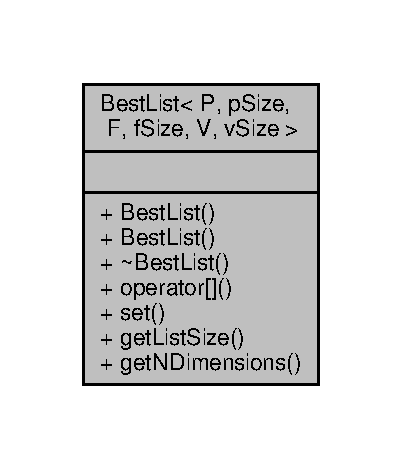
\includegraphics[width=193pt]{classBestList__coll__graph}
\end{center}
\end{figure}
\subsection*{Public Member Functions}
\begin{DoxyCompactItemize}
\item 
\hyperlink{classBestList_a4bd603848a6e66f1242323f945fedbe9}{Best\+List} (int list\+Size, int n)
\begin{DoxyCompactList}\small\item\em Constructor that generates an empty best-\/list instance. \end{DoxyCompactList}\item 
\hyperlink{classBestList_ae664f030cfdd2440bc05ef4873915d32}{Best\+List} (\hyperlink{classBestList}{Best\+List}$<$ P, p\+Size, F, f\+Size, V, v\+Size $>$ $\ast$best\+List)
\begin{DoxyCompactList}\small\item\em Constructor that generates a new best-\/list initialized as a full copy of another \hyperlink{classBestList}{Best\+List} instance. \end{DoxyCompactList}\item 
\hyperlink{classBestList_a7d0ac19666923c1c94a130a16b176125}{$\sim$\+Best\+List} ()
\begin{DoxyCompactList}\small\item\em This destructor deletes all Solutions stored in the best-\/list (i.\+e. releases their memories). \end{DoxyCompactList}\item 
\hyperlink{classSolution}{Solution}$<$ P, p\+Size, F, f\+Size, V, v\+Size $>$ $\ast$ \hyperlink{classBestList_a47b06e0c8d982f3d89769ce6b66adf0c}{operator\mbox{[}$\,$\mbox{]}} (int idx)
\begin{DoxyCompactList}\small\item\em Operator that selects a \hyperlink{classSolution}{Solution} based on its index in the list of solutions. \end{DoxyCompactList}\item 
void \hyperlink{classBestList_a4a5650fb72c71d6027540daa96de0d39}{set} (int idx, \hyperlink{classSolution}{Solution}$<$ P, p\+Size, F, f\+Size, V, v\+Size $>$ $\ast$solution)
\begin{DoxyCompactList}\small\item\em Operator to set an element in the list. \end{DoxyCompactList}\item 
int \hyperlink{classBestList_ac627a3267d2b7cf8f579cc7e5b77d2e3}{get\+List\+Size} ()
\item 
int \hyperlink{classBestList_adaf365728d0834a5f2b7f3c47dd76788}{get\+N\+Dimensions} ()
\end{DoxyCompactItemize}


\subsection{Detailed Description}
\subsubsection*{template$<$class P = double, int p\+Size = 1, class F = double, int f\+Size = 1, class V = double, int v\+Size = 1$>$\\*
class Best\+List$<$ P, p\+Size, F, f\+Size, V, v\+Size $>$}

An instance of this class holds the best-\/list for its respective \hyperlink{classTH}{TH} instance. 

\begin{DoxyAuthor}{Author}
Peter Frank Perroni 
\end{DoxyAuthor}


Definition at line 33 of file Best\+List.\+h.



\subsection{Constructor \& Destructor Documentation}
\index{Best\+List@{Best\+List}!Best\+List@{Best\+List}}
\index{Best\+List@{Best\+List}!Best\+List@{Best\+List}}
\subsubsection[{\texorpdfstring{Best\+List(int list\+Size, int n)}{BestList(int listSize, int n)}}]{\setlength{\rightskip}{0pt plus 5cm}template$<$class P = double, int p\+Size = 1, class F = double, int f\+Size = 1, class V = double, int v\+Size = 1$>$ {\bf Best\+List}$<$ P, p\+Size, F, f\+Size, V, v\+Size $>$\+::{\bf Best\+List} (
\begin{DoxyParamCaption}
\item[{int}]{list\+Size, }
\item[{int}]{n}
\end{DoxyParamCaption}
)\hspace{0.3cm}{\ttfamily [inline]}}\hypertarget{classBestList_a4bd603848a6e66f1242323f945fedbe9}{}\label{classBestList_a4bd603848a6e66f1242323f945fedbe9}


Constructor that generates an empty best-\/list instance. 


\begin{DoxyParams}{Parameters}
{\em list\+Size} & List size. \\
\hline
{\em n} & Maximum number of dimensions to be optimized. \\
\hline
\end{DoxyParams}


Definition at line 44 of file Best\+List.\+h.

\index{Best\+List@{Best\+List}!Best\+List@{Best\+List}}
\index{Best\+List@{Best\+List}!Best\+List@{Best\+List}}
\subsubsection[{\texorpdfstring{Best\+List(\+Best\+List$<$ P, p\+Size, F, f\+Size, V, v\+Size $>$ $\ast$best\+List)}{BestList(BestList< P, pSize, F, fSize, V, vSize > *bestList)}}]{\setlength{\rightskip}{0pt plus 5cm}template$<$class P = double, int p\+Size = 1, class F = double, int f\+Size = 1, class V = double, int v\+Size = 1$>$ {\bf Best\+List}$<$ P, p\+Size, F, f\+Size, V, v\+Size $>$\+::{\bf Best\+List} (
\begin{DoxyParamCaption}
\item[{{\bf Best\+List}$<$ P, p\+Size, F, f\+Size, V, v\+Size $>$ $\ast$}]{best\+List}
\end{DoxyParamCaption}
)\hspace{0.3cm}{\ttfamily [inline]}}\hypertarget{classBestList_ae664f030cfdd2440bc05ef4873915d32}{}\label{classBestList_ae664f030cfdd2440bc05ef4873915d32}


Constructor that generates a new best-\/list initialized as a full copy of another \hyperlink{classBestList}{Best\+List} instance. 


\begin{DoxyParams}{Parameters}
{\em best\+List} & The source \hyperlink{classBestList}{Best\+List} instance. \\
\hline
\end{DoxyParams}


Definition at line 56 of file Best\+List.\+h.



Here is the call graph for this function\+:
\nopagebreak
\begin{figure}[H]
\begin{center}
\leavevmode
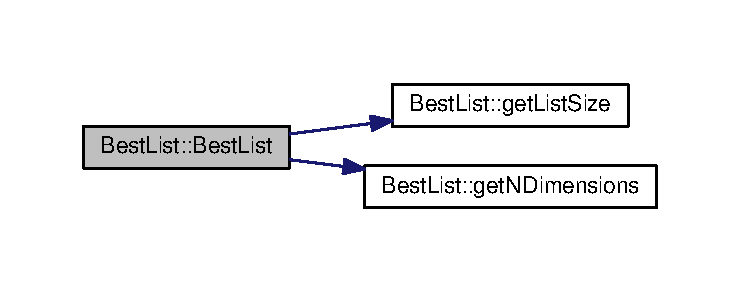
\includegraphics[width=350pt]{classBestList_ae664f030cfdd2440bc05ef4873915d32_cgraph}
\end{center}
\end{figure}


\index{Best\+List@{Best\+List}!````~Best\+List@{$\sim$\+Best\+List}}
\index{````~Best\+List@{$\sim$\+Best\+List}!Best\+List@{Best\+List}}
\subsubsection[{\texorpdfstring{$\sim$\+Best\+List()}{~BestList()}}]{\setlength{\rightskip}{0pt plus 5cm}template$<$class P = double, int p\+Size = 1, class F = double, int f\+Size = 1, class V = double, int v\+Size = 1$>$ {\bf Best\+List}$<$ P, p\+Size, F, f\+Size, V, v\+Size $>$\+::$\sim${\bf Best\+List} (
\begin{DoxyParamCaption}
{}
\end{DoxyParamCaption}
)\hspace{0.3cm}{\ttfamily [inline]}}\hypertarget{classBestList_a7d0ac19666923c1c94a130a16b176125}{}\label{classBestList_a7d0ac19666923c1c94a130a16b176125}


This destructor deletes all Solutions stored in the best-\/list (i.\+e. releases their memories). 



Definition at line 72 of file Best\+List.\+h.



\subsection{Member Function Documentation}
\index{Best\+List@{Best\+List}!get\+List\+Size@{get\+List\+Size}}
\index{get\+List\+Size@{get\+List\+Size}!Best\+List@{Best\+List}}
\subsubsection[{\texorpdfstring{get\+List\+Size()}{getListSize()}}]{\setlength{\rightskip}{0pt plus 5cm}template$<$class P = double, int p\+Size = 1, class F = double, int f\+Size = 1, class V = double, int v\+Size = 1$>$ int {\bf Best\+List}$<$ P, p\+Size, F, f\+Size, V, v\+Size $>$\+::get\+List\+Size (
\begin{DoxyParamCaption}
{}
\end{DoxyParamCaption}
)\hspace{0.3cm}{\ttfamily [inline]}}\hypertarget{classBestList_ac627a3267d2b7cf8f579cc7e5b77d2e3}{}\label{classBestList_ac627a3267d2b7cf8f579cc7e5b77d2e3}


Definition at line 108 of file Best\+List.\+h.



Here is the caller graph for this function\+:
\nopagebreak
\begin{figure}[H]
\begin{center}
\leavevmode
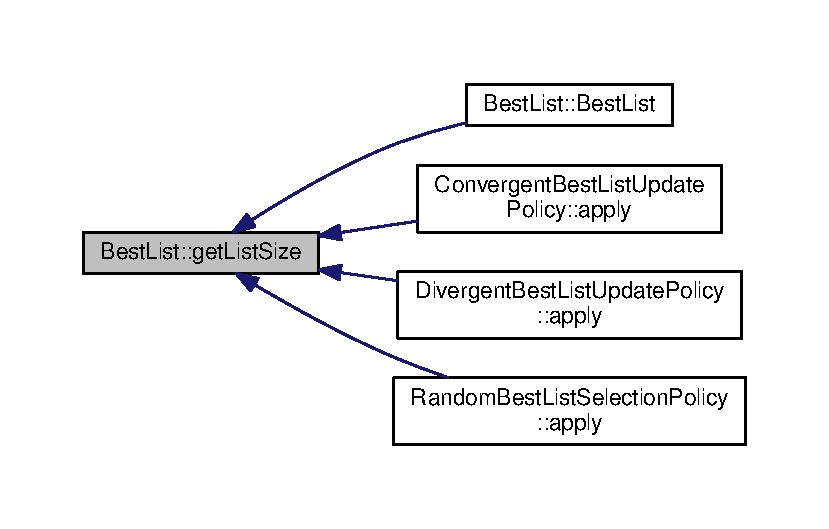
\includegraphics[width=350pt]{classBestList_ac627a3267d2b7cf8f579cc7e5b77d2e3_icgraph}
\end{center}
\end{figure}


\index{Best\+List@{Best\+List}!get\+N\+Dimensions@{get\+N\+Dimensions}}
\index{get\+N\+Dimensions@{get\+N\+Dimensions}!Best\+List@{Best\+List}}
\subsubsection[{\texorpdfstring{get\+N\+Dimensions()}{getNDimensions()}}]{\setlength{\rightskip}{0pt plus 5cm}template$<$class P = double, int p\+Size = 1, class F = double, int f\+Size = 1, class V = double, int v\+Size = 1$>$ int {\bf Best\+List}$<$ P, p\+Size, F, f\+Size, V, v\+Size $>$\+::get\+N\+Dimensions (
\begin{DoxyParamCaption}
{}
\end{DoxyParamCaption}
)\hspace{0.3cm}{\ttfamily [inline]}}\hypertarget{classBestList_adaf365728d0834a5f2b7f3c47dd76788}{}\label{classBestList_adaf365728d0834a5f2b7f3c47dd76788}


Definition at line 112 of file Best\+List.\+h.



Here is the caller graph for this function\+:
\nopagebreak
\begin{figure}[H]
\begin{center}
\leavevmode
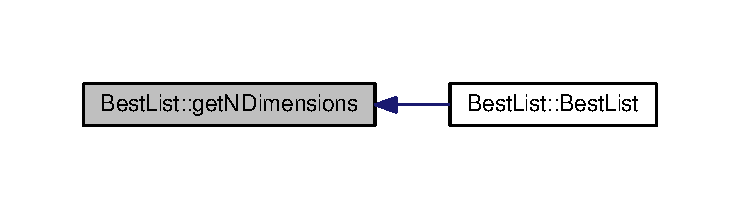
\includegraphics[width=350pt]{classBestList_adaf365728d0834a5f2b7f3c47dd76788_icgraph}
\end{center}
\end{figure}


\index{Best\+List@{Best\+List}!operator\mbox{[}$\,$\mbox{]}@{operator[]}}
\index{operator\mbox{[}$\,$\mbox{]}@{operator[]}!Best\+List@{Best\+List}}
\subsubsection[{\texorpdfstring{operator[](int idx)}{operator[](int idx)}}]{\setlength{\rightskip}{0pt plus 5cm}template$<$class P = double, int p\+Size = 1, class F = double, int f\+Size = 1, class V = double, int v\+Size = 1$>$ {\bf Solution}$<$P, p\+Size, F, f\+Size, V, v\+Size$>$$\ast$ {\bf Best\+List}$<$ P, p\+Size, F, f\+Size, V, v\+Size $>$\+::operator\mbox{[}$\,$\mbox{]} (
\begin{DoxyParamCaption}
\item[{int}]{idx}
\end{DoxyParamCaption}
)\hspace{0.3cm}{\ttfamily [inline]}}\hypertarget{classBestList_a47b06e0c8d982f3d89769ce6b66adf0c}{}\label{classBestList_a47b06e0c8d982f3d89769ce6b66adf0c}


Operator that selects a \hyperlink{classSolution}{Solution} based on its index in the list of solutions. 

The pointer to the actual object is returned, instead of a simple copy.


\begin{DoxyParams}{Parameters}
{\em idx} & The position of the \hyperlink{classSolution}{Solution} in the list (index list starts in zero). \\
\hline
\end{DoxyParams}
\begin{DoxyReturn}{Returns}
A pointer to the \hyperlink{classSolution}{Solution} selected. 
\end{DoxyReturn}


Definition at line 87 of file Best\+List.\+h.

\index{Best\+List@{Best\+List}!set@{set}}
\index{set@{set}!Best\+List@{Best\+List}}
\subsubsection[{\texorpdfstring{set(int idx, Solution$<$ P, p\+Size, F, f\+Size, V, v\+Size $>$ $\ast$solution)}{set(int idx, Solution< P, pSize, F, fSize, V, vSize > *solution)}}]{\setlength{\rightskip}{0pt plus 5cm}template$<$class P = double, int p\+Size = 1, class F = double, int f\+Size = 1, class V = double, int v\+Size = 1$>$ void {\bf Best\+List}$<$ P, p\+Size, F, f\+Size, V, v\+Size $>$\+::set (
\begin{DoxyParamCaption}
\item[{int}]{idx, }
\item[{{\bf Solution}$<$ P, p\+Size, F, f\+Size, V, v\+Size $>$ $\ast$}]{solution}
\end{DoxyParamCaption}
)\hspace{0.3cm}{\ttfamily [inline]}}\hypertarget{classBestList_a4a5650fb72c71d6027540daa96de0d39}{}\label{classBestList_a4a5650fb72c71d6027540daa96de0d39}


Operator to set an element in the list. 

The old element (if any) is deleted (i.\+e. its memory is released) and the respective index position will point to the solution received as parameter.


\begin{DoxyParams}{Parameters}
{\em idx} & The index in the list to set the new \hyperlink{classSolution}{Solution} (list starts in zero). \\
\hline
{\em solution} & The new \hyperlink{classSolution}{Solution} instance to add to the list. \\
\hline
\end{DoxyParams}


Definition at line 101 of file Best\+List.\+h.



Here is the caller graph for this function\+:
\nopagebreak
\begin{figure}[H]
\begin{center}
\leavevmode
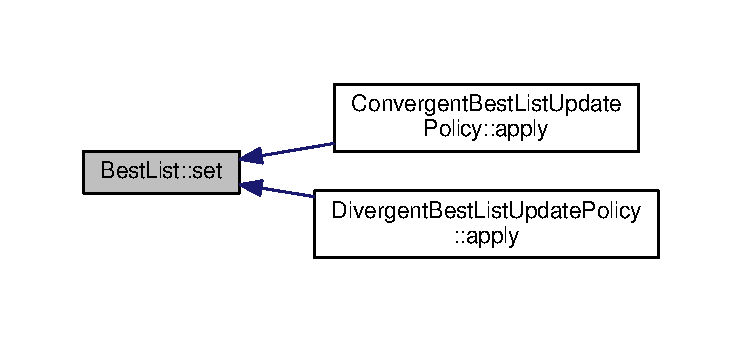
\includegraphics[width=350pt]{classBestList_a4a5650fb72c71d6027540daa96de0d39_icgraph}
\end{center}
\end{figure}




The documentation for this class was generated from the following file\+:\begin{DoxyCompactItemize}
\item 
src/\+T\+H/\hyperlink{BestList_8h}{Best\+List.\+h}\end{DoxyCompactItemize}

\hypertarget{classBestListSelectionPolicy}{}\section{Best\+List\+Selection\+Policy$<$ P, p\+Size, F, f\+Size, V, v\+Size $>$ Class Template Reference}
\label{classBestListSelectionPolicy}\index{Best\+List\+Selection\+Policy$<$ P, p\+Size, F, f\+Size, V, v\+Size $>$@{Best\+List\+Selection\+Policy$<$ P, p\+Size, F, f\+Size, V, v\+Size $>$}}


Template for the policy that specifies how a solution is selected from the \hyperlink{classBestList}{Best\+List}.  




{\ttfamily \#include $<$Best\+List\+Selection\+Policy.\+h$>$}



Inheritance diagram for Best\+List\+Selection\+Policy$<$ P, p\+Size, F, f\+Size, V, v\+Size $>$\+:\nopagebreak
\begin{figure}[H]
\begin{center}
\leavevmode
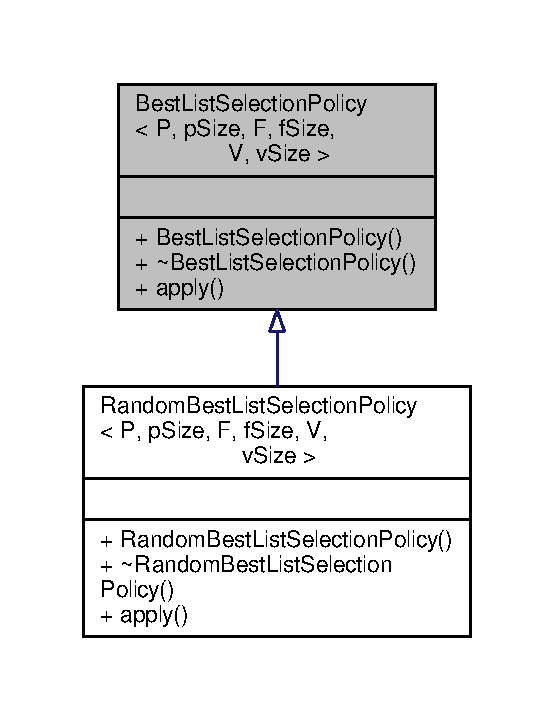
\includegraphics[width=266pt]{classBestListSelectionPolicy__inherit__graph}
\end{center}
\end{figure}


Collaboration diagram for Best\+List\+Selection\+Policy$<$ P, p\+Size, F, f\+Size, V, v\+Size $>$\+:\nopagebreak
\begin{figure}[H]
\begin{center}
\leavevmode
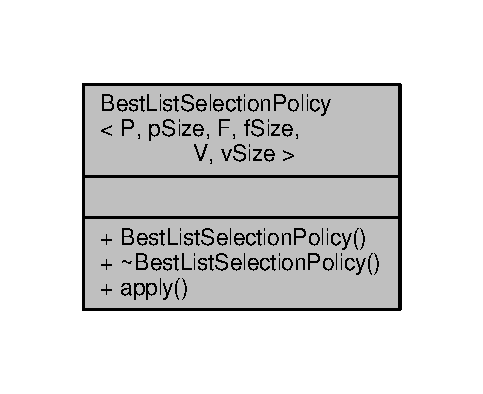
\includegraphics[width=232pt]{classBestListSelectionPolicy__coll__graph}
\end{center}
\end{figure}
\subsection*{Public Member Functions}
\begin{DoxyCompactItemize}
\item 
\hyperlink{classBestListSelectionPolicy_a20a7af0bb2e775d20048ac5eb7d624ba}{Best\+List\+Selection\+Policy} ()
\item 
virtual \hyperlink{classBestListSelectionPolicy_a9b3f3d69b8bba7506e89eaf00b4d1c08}{$\sim$\+Best\+List\+Selection\+Policy} ()
\item 
virtual \hyperlink{classSolution}{Solution}$<$ P, p\+Size, F, f\+Size, V, v\+Size $>$ $\ast$ \hyperlink{classBestListSelectionPolicy_ae387a1ef0a3a597134edf198e5ab1299}{apply} (\hyperlink{classBestList}{Best\+List}$<$ P, p\+Size, F, f\+Size, V, v\+Size $>$ $\ast$best\+List, \hyperlink{classFitnessPolicy}{Fitness\+Policy}$<$ P, p\+Size, F, f\+Size, V, v\+Size $>$ $\ast$fitness\+Policy)=0
\begin{DoxyCompactList}\small\item\em Virtual method to apply the policy that will select a solution from the best-\/list. \end{DoxyCompactList}\end{DoxyCompactItemize}


\subsection{Detailed Description}
\subsubsection*{template$<$class P = double, int p\+Size = 1, class F = double, int f\+Size = 1, class V = double, int v\+Size = 1$>$\\*
class Best\+List\+Selection\+Policy$<$ P, p\+Size, F, f\+Size, V, v\+Size $>$}

Template for the policy that specifies how a solution is selected from the \hyperlink{classBestList}{Best\+List}. 

\begin{DoxyAuthor}{Author}
Peter Frank Perroni 
\end{DoxyAuthor}


Definition at line 34 of file Best\+List\+Selection\+Policy.\+h.



\subsection{Constructor \& Destructor Documentation}
\index{Best\+List\+Selection\+Policy@{Best\+List\+Selection\+Policy}!Best\+List\+Selection\+Policy@{Best\+List\+Selection\+Policy}}
\index{Best\+List\+Selection\+Policy@{Best\+List\+Selection\+Policy}!Best\+List\+Selection\+Policy@{Best\+List\+Selection\+Policy}}
\subsubsection[{\texorpdfstring{Best\+List\+Selection\+Policy()}{BestListSelectionPolicy()}}]{\setlength{\rightskip}{0pt plus 5cm}template$<$class P = double, int p\+Size = 1, class F = double, int f\+Size = 1, class V = double, int v\+Size = 1$>$ {\bf Best\+List\+Selection\+Policy}$<$ P, p\+Size, F, f\+Size, V, v\+Size $>$\+::{\bf Best\+List\+Selection\+Policy} (
\begin{DoxyParamCaption}
{}
\end{DoxyParamCaption}
)\hspace{0.3cm}{\ttfamily [inline]}}\hypertarget{classBestListSelectionPolicy_a20a7af0bb2e775d20048ac5eb7d624ba}{}\label{classBestListSelectionPolicy_a20a7af0bb2e775d20048ac5eb7d624ba}


Definition at line 36 of file Best\+List\+Selection\+Policy.\+h.

\index{Best\+List\+Selection\+Policy@{Best\+List\+Selection\+Policy}!````~Best\+List\+Selection\+Policy@{$\sim$\+Best\+List\+Selection\+Policy}}
\index{````~Best\+List\+Selection\+Policy@{$\sim$\+Best\+List\+Selection\+Policy}!Best\+List\+Selection\+Policy@{Best\+List\+Selection\+Policy}}
\subsubsection[{\texorpdfstring{$\sim$\+Best\+List\+Selection\+Policy()}{~BestListSelectionPolicy()}}]{\setlength{\rightskip}{0pt plus 5cm}template$<$class P = double, int p\+Size = 1, class F = double, int f\+Size = 1, class V = double, int v\+Size = 1$>$ virtual {\bf Best\+List\+Selection\+Policy}$<$ P, p\+Size, F, f\+Size, V, v\+Size $>$\+::$\sim${\bf Best\+List\+Selection\+Policy} (
\begin{DoxyParamCaption}
{}
\end{DoxyParamCaption}
)\hspace{0.3cm}{\ttfamily [inline]}, {\ttfamily [virtual]}}\hypertarget{classBestListSelectionPolicy_a9b3f3d69b8bba7506e89eaf00b4d1c08}{}\label{classBestListSelectionPolicy_a9b3f3d69b8bba7506e89eaf00b4d1c08}


Definition at line 37 of file Best\+List\+Selection\+Policy.\+h.



Here is the call graph for this function\+:\nopagebreak
\begin{figure}[H]
\begin{center}
\leavevmode
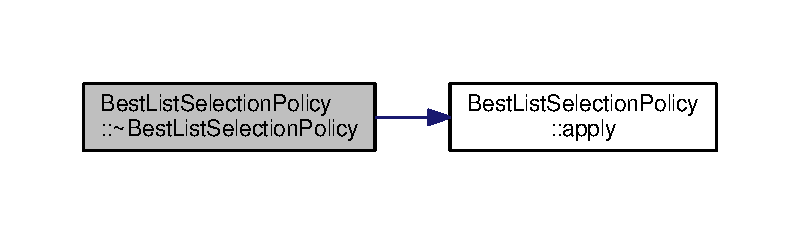
\includegraphics[width=350pt]{classBestListSelectionPolicy_a9b3f3d69b8bba7506e89eaf00b4d1c08_cgraph}
\end{center}
\end{figure}




\subsection{Member Function Documentation}
\index{Best\+List\+Selection\+Policy@{Best\+List\+Selection\+Policy}!apply@{apply}}
\index{apply@{apply}!Best\+List\+Selection\+Policy@{Best\+List\+Selection\+Policy}}
\subsubsection[{\texorpdfstring{apply(\+Best\+List$<$ P, p\+Size, F, f\+Size, V, v\+Size $>$ $\ast$best\+List, Fitness\+Policy$<$ P, p\+Size, F, f\+Size, V, v\+Size $>$ $\ast$fitness\+Policy)=0}{apply(BestList< P, pSize, F, fSize, V, vSize > *bestList, FitnessPolicy< P, pSize, F, fSize, V, vSize > *fitnessPolicy)=0}}]{\setlength{\rightskip}{0pt plus 5cm}template$<$class P = double, int p\+Size = 1, class F = double, int f\+Size = 1, class V = double, int v\+Size = 1$>$ virtual {\bf Solution}$<$P, p\+Size, F, f\+Size, V, v\+Size$>$$\ast$ {\bf Best\+List\+Selection\+Policy}$<$ P, p\+Size, F, f\+Size, V, v\+Size $>$\+::apply (
\begin{DoxyParamCaption}
\item[{{\bf Best\+List}$<$ P, p\+Size, F, f\+Size, V, v\+Size $>$ $\ast$}]{best\+List, }
\item[{{\bf Fitness\+Policy}$<$ P, p\+Size, F, f\+Size, V, v\+Size $>$ $\ast$}]{fitness\+Policy}
\end{DoxyParamCaption}
)\hspace{0.3cm}{\ttfamily [pure virtual]}}\hypertarget{classBestListSelectionPolicy_ae387a1ef0a3a597134edf198e5ab1299}{}\label{classBestListSelectionPolicy_ae387a1ef0a3a597134edf198e5ab1299}


Virtual method to apply the policy that will select a solution from the best-\/list. 

A method implementing this virtual method is the responsible for selecting and returning a solution from the best-\/list. It should use the \hyperlink{classFitnessPolicy}{Fitness\+Policy} received to compare the new solution with the solutions stored in the best-\/list.


\begin{DoxyParams}{Parameters}
{\em best\+List} & The \hyperlink{classBestList}{Best\+List} instance. \\
\hline
{\em fitness\+Policy} & The \hyperlink{classFitnessPolicy}{Fitness\+Policy} instance capable of evaluating the solutions. \\
\hline
\end{DoxyParams}
\begin{DoxyReturn}{Returns}
The solution selected by the policy. 
\end{DoxyReturn}


Implemented in \hyperlink{classRandomBestListSelectionPolicy_ae32f042697269d74c6fed4b9ff6771c8}{Random\+Best\+List\+Selection\+Policy$<$ P, p\+Size, F, f\+Size, V, v\+Size $>$}.



Here is the caller graph for this function\+:\nopagebreak
\begin{figure}[H]
\begin{center}
\leavevmode
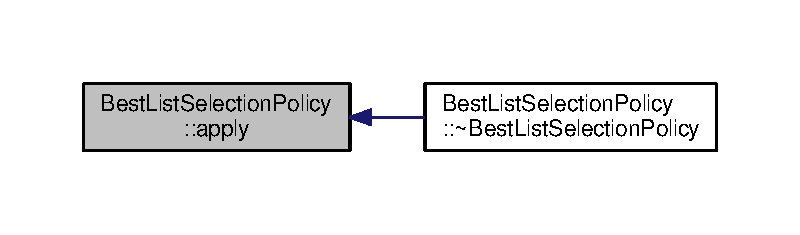
\includegraphics[width=350pt]{classBestListSelectionPolicy_ae387a1ef0a3a597134edf198e5ab1299_icgraph}
\end{center}
\end{figure}




The documentation for this class was generated from the following file\+:\begin{DoxyCompactItemize}
\item 
src/\+T\+H/\hyperlink{BestListSelectionPolicy_8h}{Best\+List\+Selection\+Policy.\+h}\end{DoxyCompactItemize}

\hypertarget{classBestListUpdatePolicy}{}\section{Best\+List\+Update\+Policy$<$ P, p\+Size, F, f\+Size, V, v\+Size $>$ Class Template Reference}
\label{classBestListUpdatePolicy}\index{Best\+List\+Update\+Policy$<$ P, p\+Size, F, f\+Size, V, v\+Size $>$@{Best\+List\+Update\+Policy$<$ P, p\+Size, F, f\+Size, V, v\+Size $>$}}


Template for the policy that specifies how the solutions within the \hyperlink{classBestList}{Best\+List} are update.  




{\ttfamily \#include $<$Best\+List\+Update\+Policy.\+h$>$}



Inheritance diagram for Best\+List\+Update\+Policy$<$ P, p\+Size, F, f\+Size, V, v\+Size $>$\+:
\nopagebreak
\begin{figure}[H]
\begin{center}
\leavevmode
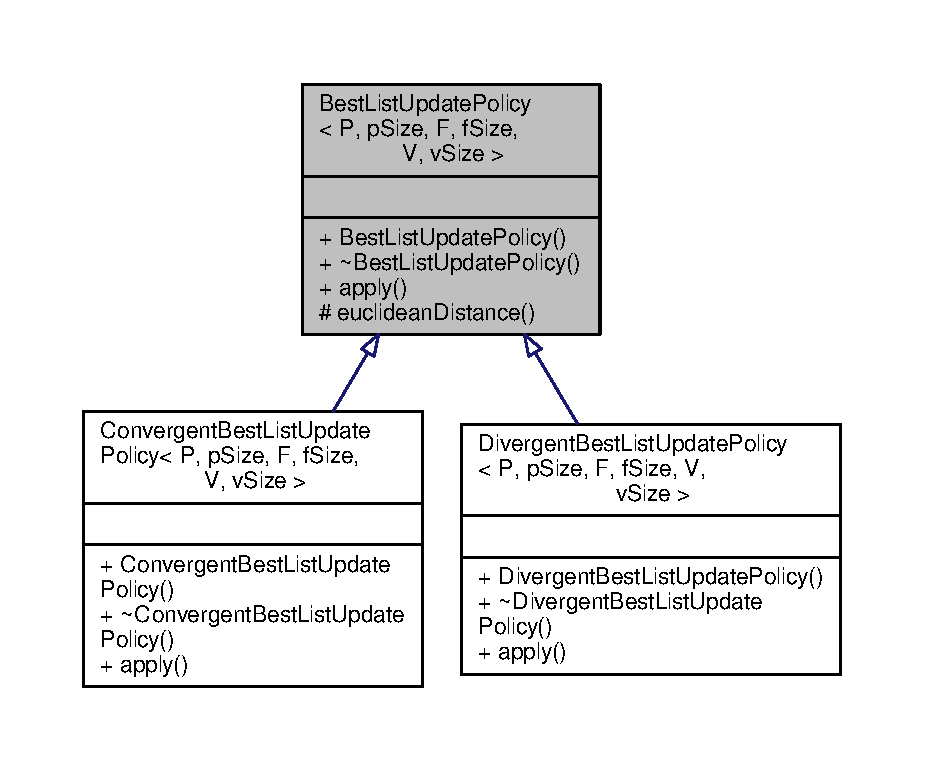
\includegraphics[width=350pt]{classBestListUpdatePolicy__inherit__graph}
\end{center}
\end{figure}


Collaboration diagram for Best\+List\+Update\+Policy$<$ P, p\+Size, F, f\+Size, V, v\+Size $>$\+:
\nopagebreak
\begin{figure}[H]
\begin{center}
\leavevmode
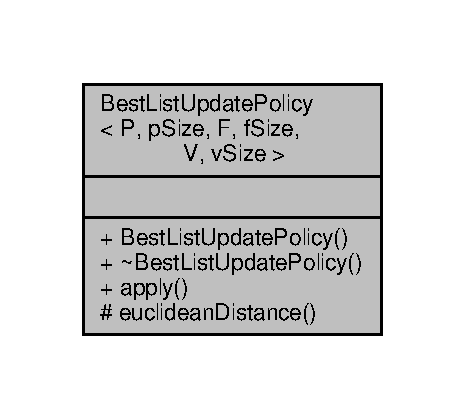
\includegraphics[width=223pt]{classBestListUpdatePolicy__coll__graph}
\end{center}
\end{figure}
\subsection*{Public Member Functions}
\begin{DoxyCompactItemize}
\item 
\hyperlink{classBestListUpdatePolicy_a0a23a636003eb43d09e16f21133459f5}{Best\+List\+Update\+Policy} ()
\item 
virtual \hyperlink{classBestListUpdatePolicy_a6c17a69a8f1c010e7ce3f524f05ec98b}{$\sim$\+Best\+List\+Update\+Policy} ()
\item 
virtual void \hyperlink{classBestListUpdatePolicy_a591442e3329323b350971b6a55195916}{apply} (\hyperlink{classBestList}{Best\+List}$<$ P, p\+Size, F, f\+Size, V, v\+Size $>$ $\ast$best\+List, \hyperlink{classSolution}{Solution}$<$ P, p\+Size, F, f\+Size, V, v\+Size $>$ $\ast$solution, \hyperlink{classFitnessPolicy}{Fitness\+Policy}$<$ P, p\+Size, F, f\+Size, V, v\+Size $>$ $\ast$fitness\+Policy)=0
\begin{DoxyCompactList}\small\item\em Virtual method to apply the policy that will update the best-\/list. \end{DoxyCompactList}\end{DoxyCompactItemize}
\subsection*{Protected Member Functions}
\begin{DoxyCompactItemize}
\item 
double \hyperlink{classBestListUpdatePolicy_a6987f90d6d9e5fec813f5aa53fe47ce3}{euclidean\+Distance} (\hyperlink{classSolution}{Solution}$<$ P, p\+Size, F, f\+Size, V, v\+Size $>$ $\ast$first, \hyperlink{classSolution}{Solution}$<$ P, p\+Size, F, f\+Size, V, v\+Size $>$ $\ast$second)
\begin{DoxyCompactList}\small\item\em Convenience method that calculates the Euclidean distance between two solutions. \end{DoxyCompactList}\end{DoxyCompactItemize}


\subsection{Detailed Description}
\subsubsection*{template$<$class P = double, int p\+Size = 1, class F = double, int f\+Size = 1, class V = double, int v\+Size = 1$>$\\*
class Best\+List\+Update\+Policy$<$ P, p\+Size, F, f\+Size, V, v\+Size $>$}

Template for the policy that specifies how the solutions within the \hyperlink{classBestList}{Best\+List} are update. 

\begin{DoxyAuthor}{Author}
Peter Frank Perroni 
\end{DoxyAuthor}


Definition at line 36 of file Best\+List\+Update\+Policy.\+h.



\subsection{Constructor \& Destructor Documentation}
\index{Best\+List\+Update\+Policy@{Best\+List\+Update\+Policy}!Best\+List\+Update\+Policy@{Best\+List\+Update\+Policy}}
\index{Best\+List\+Update\+Policy@{Best\+List\+Update\+Policy}!Best\+List\+Update\+Policy@{Best\+List\+Update\+Policy}}
\subsubsection[{\texorpdfstring{Best\+List\+Update\+Policy()}{BestListUpdatePolicy()}}]{\setlength{\rightskip}{0pt plus 5cm}template$<$class P = double, int p\+Size = 1, class F = double, int f\+Size = 1, class V = double, int v\+Size = 1$>$ {\bf Best\+List\+Update\+Policy}$<$ P, p\+Size, F, f\+Size, V, v\+Size $>$\+::{\bf Best\+List\+Update\+Policy} (
\begin{DoxyParamCaption}
{}
\end{DoxyParamCaption}
)\hspace{0.3cm}{\ttfamily [inline]}}\hypertarget{classBestListUpdatePolicy_a0a23a636003eb43d09e16f21133459f5}{}\label{classBestListUpdatePolicy_a0a23a636003eb43d09e16f21133459f5}


Definition at line 63 of file Best\+List\+Update\+Policy.\+h.

\index{Best\+List\+Update\+Policy@{Best\+List\+Update\+Policy}!````~Best\+List\+Update\+Policy@{$\sim$\+Best\+List\+Update\+Policy}}
\index{````~Best\+List\+Update\+Policy@{$\sim$\+Best\+List\+Update\+Policy}!Best\+List\+Update\+Policy@{Best\+List\+Update\+Policy}}
\subsubsection[{\texorpdfstring{$\sim$\+Best\+List\+Update\+Policy()}{~BestListUpdatePolicy()}}]{\setlength{\rightskip}{0pt plus 5cm}template$<$class P = double, int p\+Size = 1, class F = double, int f\+Size = 1, class V = double, int v\+Size = 1$>$ virtual {\bf Best\+List\+Update\+Policy}$<$ P, p\+Size, F, f\+Size, V, v\+Size $>$\+::$\sim${\bf Best\+List\+Update\+Policy} (
\begin{DoxyParamCaption}
{}
\end{DoxyParamCaption}
)\hspace{0.3cm}{\ttfamily [inline]}, {\ttfamily [virtual]}}\hypertarget{classBestListUpdatePolicy_a6c17a69a8f1c010e7ce3f524f05ec98b}{}\label{classBestListUpdatePolicy_a6c17a69a8f1c010e7ce3f524f05ec98b}


Definition at line 64 of file Best\+List\+Update\+Policy.\+h.



Here is the call graph for this function\+:
\nopagebreak
\begin{figure}[H]
\begin{center}
\leavevmode
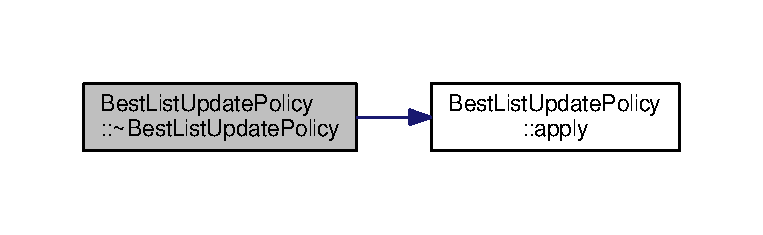
\includegraphics[width=350pt]{classBestListUpdatePolicy_a6c17a69a8f1c010e7ce3f524f05ec98b_cgraph}
\end{center}
\end{figure}




\subsection{Member Function Documentation}
\index{Best\+List\+Update\+Policy@{Best\+List\+Update\+Policy}!apply@{apply}}
\index{apply@{apply}!Best\+List\+Update\+Policy@{Best\+List\+Update\+Policy}}
\subsubsection[{\texorpdfstring{apply(\+Best\+List$<$ P, p\+Size, F, f\+Size, V, v\+Size $>$ $\ast$best\+List, Solution$<$ P, p\+Size, F, f\+Size, V, v\+Size $>$ $\ast$solution, Fitness\+Policy$<$ P, p\+Size, F, f\+Size, V, v\+Size $>$ $\ast$fitness\+Policy)=0}{apply(BestList< P, pSize, F, fSize, V, vSize > *bestList, Solution< P, pSize, F, fSize, V, vSize > *solution, FitnessPolicy< P, pSize, F, fSize, V, vSize > *fitnessPolicy)=0}}]{\setlength{\rightskip}{0pt plus 5cm}template$<$class P = double, int p\+Size = 1, class F = double, int f\+Size = 1, class V = double, int v\+Size = 1$>$ virtual void {\bf Best\+List\+Update\+Policy}$<$ P, p\+Size, F, f\+Size, V, v\+Size $>$\+::apply (
\begin{DoxyParamCaption}
\item[{{\bf Best\+List}$<$ P, p\+Size, F, f\+Size, V, v\+Size $>$ $\ast$}]{best\+List, }
\item[{{\bf Solution}$<$ P, p\+Size, F, f\+Size, V, v\+Size $>$ $\ast$}]{solution, }
\item[{{\bf Fitness\+Policy}$<$ P, p\+Size, F, f\+Size, V, v\+Size $>$ $\ast$}]{fitness\+Policy}
\end{DoxyParamCaption}
)\hspace{0.3cm}{\ttfamily [pure virtual]}}\hypertarget{classBestListUpdatePolicy_a591442e3329323b350971b6a55195916}{}\label{classBestListUpdatePolicy_a591442e3329323b350971b6a55195916}


Virtual method to apply the policy that will update the best-\/list. 

A method implementing this virtual method is the responsible for actually updating the best-\/list. It should use the \hyperlink{classFitnessPolicy}{Fitness\+Policy} received to compare the new solution with the solutions stored in the best-\/list.


\begin{DoxyParams}{Parameters}
{\em best\+List} & The \hyperlink{classBestList}{Best\+List} instance to be updated. \\
\hline
{\em solution} & The new solution to be added to the best-\/list. \\
\hline
{\em fitness\+Policy} & The \hyperlink{classFitnessPolicy}{Fitness\+Policy} instance capable of evaluating the solutions. \\
\hline
\end{DoxyParams}


Implemented in \hyperlink{classConvergentBestListUpdatePolicy_a6382937d32ac8bab7169f216fcd3048f}{Convergent\+Best\+List\+Update\+Policy$<$ P, p\+Size, F, f\+Size, V, v\+Size $>$}, and \hyperlink{classDivergentBestListUpdatePolicy_a793d47a0c458eef94b27fbee73e5df0e}{Divergent\+Best\+List\+Update\+Policy$<$ P, p\+Size, F, f\+Size, V, v\+Size $>$}.



Here is the caller graph for this function\+:
\nopagebreak
\begin{figure}[H]
\begin{center}
\leavevmode

\includegraphics[width=350pt]{classBestListUpdatePolicy_a591442e3329323b350971b6a55195916_icgraph}
\end{center}
\end{figure}


\index{Best\+List\+Update\+Policy@{Best\+List\+Update\+Policy}!euclidean\+Distance@{euclidean\+Distance}}
\index{euclidean\+Distance@{euclidean\+Distance}!Best\+List\+Update\+Policy@{Best\+List\+Update\+Policy}}
\subsubsection[{\texorpdfstring{euclidean\+Distance(\+Solution$<$ P, p\+Size, F, f\+Size, V, v\+Size $>$ $\ast$first, Solution$<$ P, p\+Size, F, f\+Size, V, v\+Size $>$ $\ast$second)}{euclideanDistance(Solution< P, pSize, F, fSize, V, vSize > *first, Solution< P, pSize, F, fSize, V, vSize > *second)}}]{\setlength{\rightskip}{0pt plus 5cm}template$<$class P = double, int p\+Size = 1, class F = double, int f\+Size = 1, class V = double, int v\+Size = 1$>$ double {\bf Best\+List\+Update\+Policy}$<$ P, p\+Size, F, f\+Size, V, v\+Size $>$\+::euclidean\+Distance (
\begin{DoxyParamCaption}
\item[{{\bf Solution}$<$ P, p\+Size, F, f\+Size, V, v\+Size $>$ $\ast$}]{first, }
\item[{{\bf Solution}$<$ P, p\+Size, F, f\+Size, V, v\+Size $>$ $\ast$}]{second}
\end{DoxyParamCaption}
)\hspace{0.3cm}{\ttfamily [inline]}, {\ttfamily [protected]}}\hypertarget{classBestListUpdatePolicy_a6987f90d6d9e5fec813f5aa53fe47ce3}{}\label{classBestListUpdatePolicy_a6987f90d6d9e5fec813f5aa53fe47ce3}


Convenience method that calculates the Euclidean distance between two solutions. 


\begin{DoxyParams}{Parameters}
{\em first} & The first solution. \\
\hline
{\em second} & The second solution. \\
\hline
\end{DoxyParams}
\begin{DoxyReturn}{Returns}
A double number representing the Euclidean distance between the solutions. 
\end{DoxyReturn}


Definition at line 44 of file Best\+List\+Update\+Policy.\+h.



Here is the call graph for this function\+:
\nopagebreak
\begin{figure}[H]
\begin{center}
\leavevmode
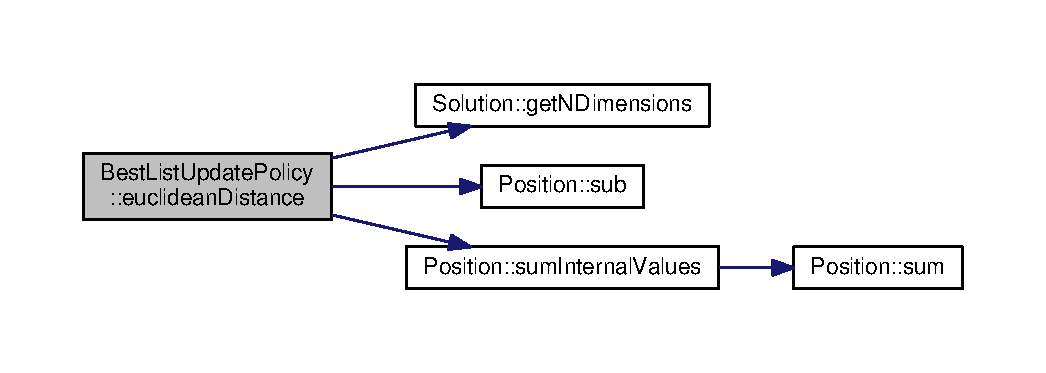
\includegraphics[width=350pt]{classBestListUpdatePolicy_a6987f90d6d9e5fec813f5aa53fe47ce3_cgraph}
\end{center}
\end{figure}




Here is the caller graph for this function\+:
\nopagebreak
\begin{figure}[H]
\begin{center}
\leavevmode
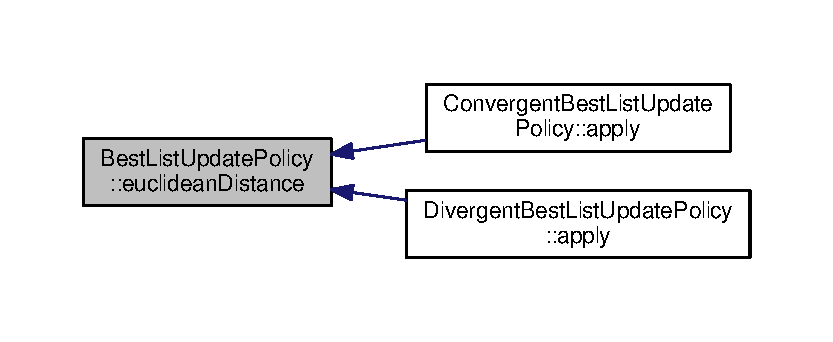
\includegraphics[width=350pt]{classBestListUpdatePolicy_a6987f90d6d9e5fec813f5aa53fe47ce3_icgraph}
\end{center}
\end{figure}




The documentation for this class was generated from the following file\+:\begin{DoxyCompactItemize}
\item 
src/\+T\+H/\hyperlink{BestListUpdatePolicy_8h}{Best\+List\+Update\+Policy.\+h}\end{DoxyCompactItemize}

\hypertarget{structBetaRelocationStrategyData}{}\section{Beta\+Relocation\+Strategy\+Data$<$ P, p\+Size, F, f\+Size, V, v\+Size $>$ Class Template Reference}
\label{structBetaRelocationStrategyData}\index{Beta\+Relocation\+Strategy\+Data$<$ P, p\+Size, F, f\+Size, V, v\+Size $>$@{Beta\+Relocation\+Strategy\+Data$<$ P, p\+Size, F, f\+Size, V, v\+Size $>$}}


This class is a repository containing useful data to perform the Beta-\/relocation strategy.  




{\ttfamily \#include $<$Beta\+Relocation\+Strategy\+Data.\+h$>$}



Inheritance diagram for Beta\+Relocation\+Strategy\+Data$<$ P, p\+Size, F, f\+Size, V, v\+Size $>$\+:
\nopagebreak
\begin{figure}[H]
\begin{center}
\leavevmode
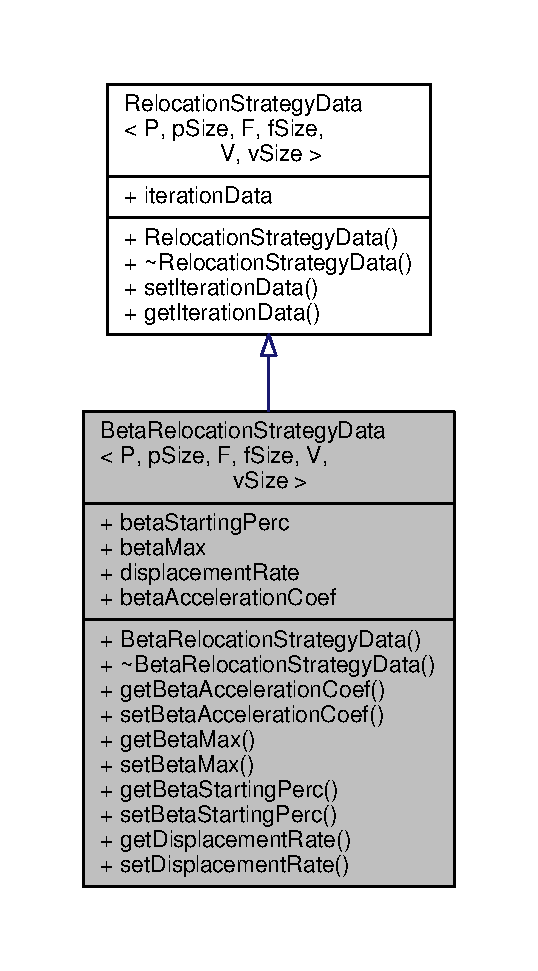
\includegraphics[width=258pt]{structBetaRelocationStrategyData__inherit__graph}
\end{center}
\end{figure}


Collaboration diagram for Beta\+Relocation\+Strategy\+Data$<$ P, p\+Size, F, f\+Size, V, v\+Size $>$\+:
\nopagebreak
\begin{figure}[H]
\begin{center}
\leavevmode
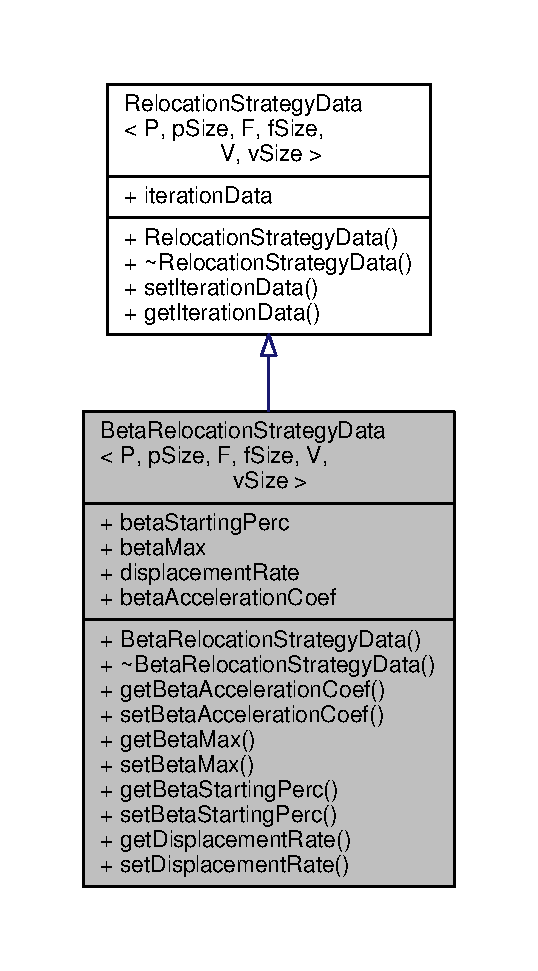
\includegraphics[width=258pt]{structBetaRelocationStrategyData__coll__graph}
\end{center}
\end{figure}
\subsection*{Public Member Functions}
\begin{DoxyCompactItemize}
\item 
\hyperlink{structBetaRelocationStrategyData_aa8b0b5da68740b089a3e7623b912ce94}{Beta\+Relocation\+Strategy\+Data} (double \hyperlink{structBetaRelocationStrategyData_a979c9c710b41d2d745ef519b4eff2b9b}{beta\+Starting\+Perc}, double \hyperlink{structBetaRelocationStrategyData_acfd06a41587b792b0f85807fe800b46a}{beta\+Max}, double \hyperlink{structBetaRelocationStrategyData_a92704a1adaddfe1d7545fd3f1c921fcd}{displacement\+Rate}, double \hyperlink{structBetaRelocationStrategyData_a957ba3439a50f2dadf2e500ac0cfcd3c}{beta\+Acceleration\+Coef})
\item 
\hyperlink{structBetaRelocationStrategyData_aba59c29006f208b6aa9694f11cefbb3b}{$\sim$\+Beta\+Relocation\+Strategy\+Data} ()
\item 
double \hyperlink{structBetaRelocationStrategyData_aabba2baebc6e6b1eebc7ab84f3ceeb5b}{get\+Beta\+Acceleration\+Coef} ()
\item 
void \hyperlink{structBetaRelocationStrategyData_a217653e9479fd18e2d32e95ba8f2b5ba}{set\+Beta\+Acceleration\+Coef} (double \hyperlink{structBetaRelocationStrategyData_a957ba3439a50f2dadf2e500ac0cfcd3c}{beta\+Acceleration\+Coef})
\item 
double \hyperlink{structBetaRelocationStrategyData_a29fa5c11b663b88ed1771a603a0fc230}{get\+Beta\+Max} ()
\item 
void \hyperlink{structBetaRelocationStrategyData_ab46e2b4b27320698671e4c4b113cb2a8}{set\+Beta\+Max} (double \hyperlink{structBetaRelocationStrategyData_acfd06a41587b792b0f85807fe800b46a}{beta\+Max})
\item 
double \hyperlink{structBetaRelocationStrategyData_a28b664079989690fdc9f56927807b3a8}{get\+Beta\+Starting\+Perc} ()
\item 
void \hyperlink{structBetaRelocationStrategyData_aa49e61c2d389efdecd637a3325cc5a2e}{set\+Beta\+Starting\+Perc} (double \hyperlink{structBetaRelocationStrategyData_a979c9c710b41d2d745ef519b4eff2b9b}{beta\+Starting\+Perc})
\item 
double \hyperlink{structBetaRelocationStrategyData_a96c3430655d3b0c2d0a41fe6515fbf18}{get\+Displacement\+Rate} ()
\item 
void \hyperlink{structBetaRelocationStrategyData_a542d95263cbcd95c32b43f31881331a5}{set\+Displacement\+Rate} (double \hyperlink{structBetaRelocationStrategyData_a92704a1adaddfe1d7545fd3f1c921fcd}{displacement\+Rate})
\end{DoxyCompactItemize}
\subsection*{Data Fields}
\begin{DoxyCompactItemize}
\item 
double \hyperlink{structBetaRelocationStrategyData_a979c9c710b41d2d745ef519b4eff2b9b}{beta\+Starting\+Perc}
\item 
double \hyperlink{structBetaRelocationStrategyData_acfd06a41587b792b0f85807fe800b46a}{beta\+Max}
\item 
double \hyperlink{structBetaRelocationStrategyData_a92704a1adaddfe1d7545fd3f1c921fcd}{displacement\+Rate}
\item 
double \hyperlink{structBetaRelocationStrategyData_a957ba3439a50f2dadf2e500ac0cfcd3c}{beta\+Acceleration\+Coef}
\end{DoxyCompactItemize}


\subsection{Detailed Description}
\subsubsection*{template$<$class P = double, int p\+Size = 1, class F = double, int f\+Size = 1, class V = double, int v\+Size = 1$>$\\*
class Beta\+Relocation\+Strategy\+Data$<$ P, p\+Size, F, f\+Size, V, v\+Size $>$}

This class is a repository containing useful data to perform the Beta-\/relocation strategy. 

\begin{DoxyAuthor}{Author}
Peter Frank Perroni 
\end{DoxyAuthor}


Definition at line 34 of file Beta\+Relocation\+Strategy\+Data.\+h.



\subsection{Constructor \& Destructor Documentation}
\index{Beta\+Relocation\+Strategy\+Data@{Beta\+Relocation\+Strategy\+Data}!Beta\+Relocation\+Strategy\+Data@{Beta\+Relocation\+Strategy\+Data}}
\index{Beta\+Relocation\+Strategy\+Data@{Beta\+Relocation\+Strategy\+Data}!Beta\+Relocation\+Strategy\+Data@{Beta\+Relocation\+Strategy\+Data}}
\subsubsection[{\texorpdfstring{Beta\+Relocation\+Strategy\+Data(double beta\+Starting\+Perc, double beta\+Max, double displacement\+Rate, double beta\+Acceleration\+Coef)}{BetaRelocationStrategyData(double betaStartingPerc, double betaMax, double displacementRate, double betaAccelerationCoef)}}]{\setlength{\rightskip}{0pt plus 5cm}template$<$class P = double, int p\+Size = 1, class F = double, int f\+Size = 1, class V = double, int v\+Size = 1$>$ {\bf Beta\+Relocation\+Strategy\+Data}$<$ P, p\+Size, F, f\+Size, V, v\+Size $>$\+::{\bf Beta\+Relocation\+Strategy\+Data} (
\begin{DoxyParamCaption}
\item[{double}]{beta\+Starting\+Perc, }
\item[{double}]{beta\+Max, }
\item[{double}]{displacement\+Rate, }
\item[{double}]{beta\+Acceleration\+Coef}
\end{DoxyParamCaption}
)\hspace{0.3cm}{\ttfamily [inline]}}\hypertarget{structBetaRelocationStrategyData_aa8b0b5da68740b089a3e7623b912ce94}{}\label{structBetaRelocationStrategyData_aa8b0b5da68740b089a3e7623b912ce94}


Definition at line 41 of file Beta\+Relocation\+Strategy\+Data.\+h.

\index{Beta\+Relocation\+Strategy\+Data@{Beta\+Relocation\+Strategy\+Data}!````~Beta\+Relocation\+Strategy\+Data@{$\sim$\+Beta\+Relocation\+Strategy\+Data}}
\index{````~Beta\+Relocation\+Strategy\+Data@{$\sim$\+Beta\+Relocation\+Strategy\+Data}!Beta\+Relocation\+Strategy\+Data@{Beta\+Relocation\+Strategy\+Data}}
\subsubsection[{\texorpdfstring{$\sim$\+Beta\+Relocation\+Strategy\+Data()}{~BetaRelocationStrategyData()}}]{\setlength{\rightskip}{0pt plus 5cm}template$<$class P = double, int p\+Size = 1, class F = double, int f\+Size = 1, class V = double, int v\+Size = 1$>$ {\bf Beta\+Relocation\+Strategy\+Data}$<$ P, p\+Size, F, f\+Size, V, v\+Size $>$\+::$\sim${\bf Beta\+Relocation\+Strategy\+Data} (
\begin{DoxyParamCaption}
{}
\end{DoxyParamCaption}
)\hspace{0.3cm}{\ttfamily [inline]}}\hypertarget{structBetaRelocationStrategyData_aba59c29006f208b6aa9694f11cefbb3b}{}\label{structBetaRelocationStrategyData_aba59c29006f208b6aa9694f11cefbb3b}


Definition at line 47 of file Beta\+Relocation\+Strategy\+Data.\+h.



\subsection{Member Function Documentation}
\index{Beta\+Relocation\+Strategy\+Data@{Beta\+Relocation\+Strategy\+Data}!get\+Beta\+Acceleration\+Coef@{get\+Beta\+Acceleration\+Coef}}
\index{get\+Beta\+Acceleration\+Coef@{get\+Beta\+Acceleration\+Coef}!Beta\+Relocation\+Strategy\+Data@{Beta\+Relocation\+Strategy\+Data}}
\subsubsection[{\texorpdfstring{get\+Beta\+Acceleration\+Coef()}{getBetaAccelerationCoef()}}]{\setlength{\rightskip}{0pt plus 5cm}template$<$class P = double, int p\+Size = 1, class F = double, int f\+Size = 1, class V = double, int v\+Size = 1$>$ double {\bf Beta\+Relocation\+Strategy\+Data}$<$ P, p\+Size, F, f\+Size, V, v\+Size $>$\+::get\+Beta\+Acceleration\+Coef (
\begin{DoxyParamCaption}
{}
\end{DoxyParamCaption}
)\hspace{0.3cm}{\ttfamily [inline]}}\hypertarget{structBetaRelocationStrategyData_aabba2baebc6e6b1eebc7ab84f3ceeb5b}{}\label{structBetaRelocationStrategyData_aabba2baebc6e6b1eebc7ab84f3ceeb5b}


Definition at line 49 of file Beta\+Relocation\+Strategy\+Data.\+h.



Here is the caller graph for this function\+:
\nopagebreak
\begin{figure}[H]
\begin{center}
\leavevmode
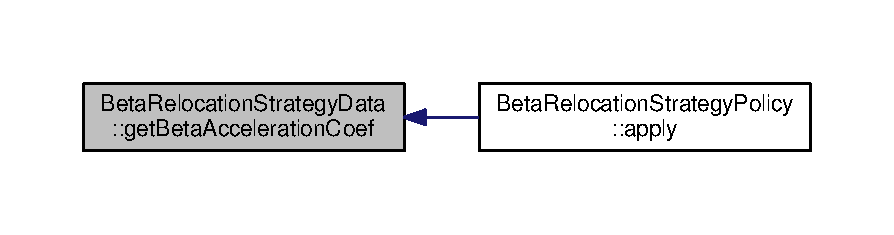
\includegraphics[width=350pt]{structBetaRelocationStrategyData_aabba2baebc6e6b1eebc7ab84f3ceeb5b_icgraph}
\end{center}
\end{figure}


\index{Beta\+Relocation\+Strategy\+Data@{Beta\+Relocation\+Strategy\+Data}!get\+Beta\+Max@{get\+Beta\+Max}}
\index{get\+Beta\+Max@{get\+Beta\+Max}!Beta\+Relocation\+Strategy\+Data@{Beta\+Relocation\+Strategy\+Data}}
\subsubsection[{\texorpdfstring{get\+Beta\+Max()}{getBetaMax()}}]{\setlength{\rightskip}{0pt plus 5cm}template$<$class P = double, int p\+Size = 1, class F = double, int f\+Size = 1, class V = double, int v\+Size = 1$>$ double {\bf Beta\+Relocation\+Strategy\+Data}$<$ P, p\+Size, F, f\+Size, V, v\+Size $>$\+::get\+Beta\+Max (
\begin{DoxyParamCaption}
{}
\end{DoxyParamCaption}
)\hspace{0.3cm}{\ttfamily [inline]}}\hypertarget{structBetaRelocationStrategyData_a29fa5c11b663b88ed1771a603a0fc230}{}\label{structBetaRelocationStrategyData_a29fa5c11b663b88ed1771a603a0fc230}


Definition at line 57 of file Beta\+Relocation\+Strategy\+Data.\+h.



Here is the caller graph for this function\+:
\nopagebreak
\begin{figure}[H]
\begin{center}
\leavevmode
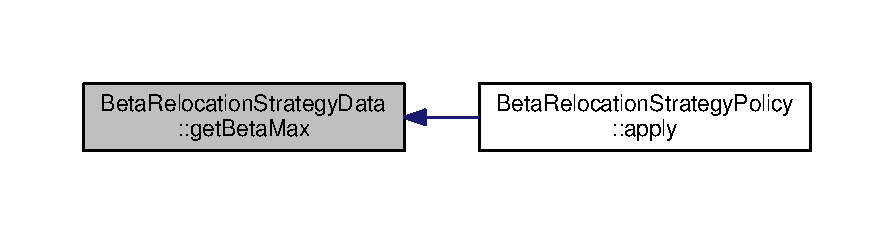
\includegraphics[width=350pt]{structBetaRelocationStrategyData_a29fa5c11b663b88ed1771a603a0fc230_icgraph}
\end{center}
\end{figure}


\index{Beta\+Relocation\+Strategy\+Data@{Beta\+Relocation\+Strategy\+Data}!get\+Beta\+Starting\+Perc@{get\+Beta\+Starting\+Perc}}
\index{get\+Beta\+Starting\+Perc@{get\+Beta\+Starting\+Perc}!Beta\+Relocation\+Strategy\+Data@{Beta\+Relocation\+Strategy\+Data}}
\subsubsection[{\texorpdfstring{get\+Beta\+Starting\+Perc()}{getBetaStartingPerc()}}]{\setlength{\rightskip}{0pt plus 5cm}template$<$class P = double, int p\+Size = 1, class F = double, int f\+Size = 1, class V = double, int v\+Size = 1$>$ double {\bf Beta\+Relocation\+Strategy\+Data}$<$ P, p\+Size, F, f\+Size, V, v\+Size $>$\+::get\+Beta\+Starting\+Perc (
\begin{DoxyParamCaption}
{}
\end{DoxyParamCaption}
)\hspace{0.3cm}{\ttfamily [inline]}}\hypertarget{structBetaRelocationStrategyData_a28b664079989690fdc9f56927807b3a8}{}\label{structBetaRelocationStrategyData_a28b664079989690fdc9f56927807b3a8}


Definition at line 65 of file Beta\+Relocation\+Strategy\+Data.\+h.



Here is the caller graph for this function\+:
\nopagebreak
\begin{figure}[H]
\begin{center}
\leavevmode
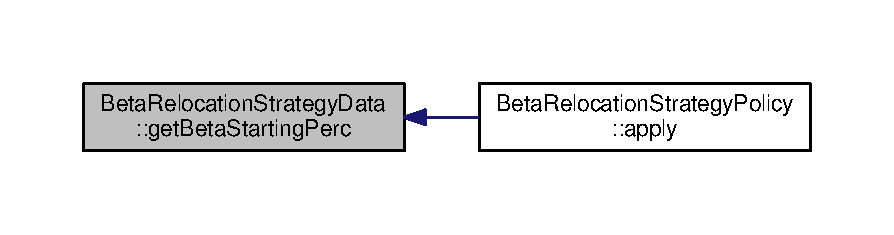
\includegraphics[width=350pt]{structBetaRelocationStrategyData_a28b664079989690fdc9f56927807b3a8_icgraph}
\end{center}
\end{figure}


\index{Beta\+Relocation\+Strategy\+Data@{Beta\+Relocation\+Strategy\+Data}!get\+Displacement\+Rate@{get\+Displacement\+Rate}}
\index{get\+Displacement\+Rate@{get\+Displacement\+Rate}!Beta\+Relocation\+Strategy\+Data@{Beta\+Relocation\+Strategy\+Data}}
\subsubsection[{\texorpdfstring{get\+Displacement\+Rate()}{getDisplacementRate()}}]{\setlength{\rightskip}{0pt plus 5cm}template$<$class P = double, int p\+Size = 1, class F = double, int f\+Size = 1, class V = double, int v\+Size = 1$>$ double {\bf Beta\+Relocation\+Strategy\+Data}$<$ P, p\+Size, F, f\+Size, V, v\+Size $>$\+::get\+Displacement\+Rate (
\begin{DoxyParamCaption}
{}
\end{DoxyParamCaption}
)\hspace{0.3cm}{\ttfamily [inline]}}\hypertarget{structBetaRelocationStrategyData_a96c3430655d3b0c2d0a41fe6515fbf18}{}\label{structBetaRelocationStrategyData_a96c3430655d3b0c2d0a41fe6515fbf18}


Definition at line 73 of file Beta\+Relocation\+Strategy\+Data.\+h.



Here is the caller graph for this function\+:
\nopagebreak
\begin{figure}[H]
\begin{center}
\leavevmode
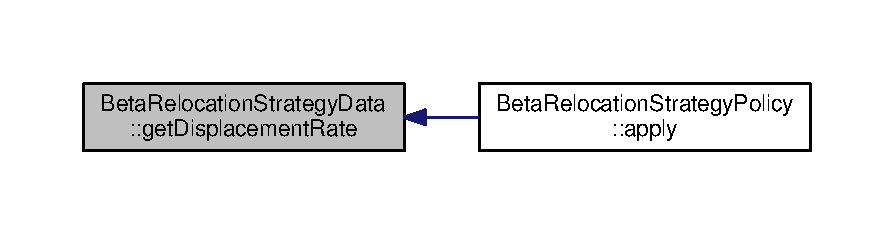
\includegraphics[width=350pt]{structBetaRelocationStrategyData_a96c3430655d3b0c2d0a41fe6515fbf18_icgraph}
\end{center}
\end{figure}


\index{Beta\+Relocation\+Strategy\+Data@{Beta\+Relocation\+Strategy\+Data}!set\+Beta\+Acceleration\+Coef@{set\+Beta\+Acceleration\+Coef}}
\index{set\+Beta\+Acceleration\+Coef@{set\+Beta\+Acceleration\+Coef}!Beta\+Relocation\+Strategy\+Data@{Beta\+Relocation\+Strategy\+Data}}
\subsubsection[{\texorpdfstring{set\+Beta\+Acceleration\+Coef(double beta\+Acceleration\+Coef)}{setBetaAccelerationCoef(double betaAccelerationCoef)}}]{\setlength{\rightskip}{0pt plus 5cm}template$<$class P = double, int p\+Size = 1, class F = double, int f\+Size = 1, class V = double, int v\+Size = 1$>$ void {\bf Beta\+Relocation\+Strategy\+Data}$<$ P, p\+Size, F, f\+Size, V, v\+Size $>$\+::set\+Beta\+Acceleration\+Coef (
\begin{DoxyParamCaption}
\item[{double}]{beta\+Acceleration\+Coef}
\end{DoxyParamCaption}
)\hspace{0.3cm}{\ttfamily [inline]}}\hypertarget{structBetaRelocationStrategyData_a217653e9479fd18e2d32e95ba8f2b5ba}{}\label{structBetaRelocationStrategyData_a217653e9479fd18e2d32e95ba8f2b5ba}


Definition at line 53 of file Beta\+Relocation\+Strategy\+Data.\+h.

\index{Beta\+Relocation\+Strategy\+Data@{Beta\+Relocation\+Strategy\+Data}!set\+Beta\+Max@{set\+Beta\+Max}}
\index{set\+Beta\+Max@{set\+Beta\+Max}!Beta\+Relocation\+Strategy\+Data@{Beta\+Relocation\+Strategy\+Data}}
\subsubsection[{\texorpdfstring{set\+Beta\+Max(double beta\+Max)}{setBetaMax(double betaMax)}}]{\setlength{\rightskip}{0pt plus 5cm}template$<$class P = double, int p\+Size = 1, class F = double, int f\+Size = 1, class V = double, int v\+Size = 1$>$ void {\bf Beta\+Relocation\+Strategy\+Data}$<$ P, p\+Size, F, f\+Size, V, v\+Size $>$\+::set\+Beta\+Max (
\begin{DoxyParamCaption}
\item[{double}]{beta\+Max}
\end{DoxyParamCaption}
)\hspace{0.3cm}{\ttfamily [inline]}}\hypertarget{structBetaRelocationStrategyData_ab46e2b4b27320698671e4c4b113cb2a8}{}\label{structBetaRelocationStrategyData_ab46e2b4b27320698671e4c4b113cb2a8}


Definition at line 61 of file Beta\+Relocation\+Strategy\+Data.\+h.

\index{Beta\+Relocation\+Strategy\+Data@{Beta\+Relocation\+Strategy\+Data}!set\+Beta\+Starting\+Perc@{set\+Beta\+Starting\+Perc}}
\index{set\+Beta\+Starting\+Perc@{set\+Beta\+Starting\+Perc}!Beta\+Relocation\+Strategy\+Data@{Beta\+Relocation\+Strategy\+Data}}
\subsubsection[{\texorpdfstring{set\+Beta\+Starting\+Perc(double beta\+Starting\+Perc)}{setBetaStartingPerc(double betaStartingPerc)}}]{\setlength{\rightskip}{0pt plus 5cm}template$<$class P = double, int p\+Size = 1, class F = double, int f\+Size = 1, class V = double, int v\+Size = 1$>$ void {\bf Beta\+Relocation\+Strategy\+Data}$<$ P, p\+Size, F, f\+Size, V, v\+Size $>$\+::set\+Beta\+Starting\+Perc (
\begin{DoxyParamCaption}
\item[{double}]{beta\+Starting\+Perc}
\end{DoxyParamCaption}
)\hspace{0.3cm}{\ttfamily [inline]}}\hypertarget{structBetaRelocationStrategyData_aa49e61c2d389efdecd637a3325cc5a2e}{}\label{structBetaRelocationStrategyData_aa49e61c2d389efdecd637a3325cc5a2e}


Definition at line 69 of file Beta\+Relocation\+Strategy\+Data.\+h.

\index{Beta\+Relocation\+Strategy\+Data@{Beta\+Relocation\+Strategy\+Data}!set\+Displacement\+Rate@{set\+Displacement\+Rate}}
\index{set\+Displacement\+Rate@{set\+Displacement\+Rate}!Beta\+Relocation\+Strategy\+Data@{Beta\+Relocation\+Strategy\+Data}}
\subsubsection[{\texorpdfstring{set\+Displacement\+Rate(double displacement\+Rate)}{setDisplacementRate(double displacementRate)}}]{\setlength{\rightskip}{0pt plus 5cm}template$<$class P = double, int p\+Size = 1, class F = double, int f\+Size = 1, class V = double, int v\+Size = 1$>$ void {\bf Beta\+Relocation\+Strategy\+Data}$<$ P, p\+Size, F, f\+Size, V, v\+Size $>$\+::set\+Displacement\+Rate (
\begin{DoxyParamCaption}
\item[{double}]{displacement\+Rate}
\end{DoxyParamCaption}
)\hspace{0.3cm}{\ttfamily [inline]}}\hypertarget{structBetaRelocationStrategyData_a542d95263cbcd95c32b43f31881331a5}{}\label{structBetaRelocationStrategyData_a542d95263cbcd95c32b43f31881331a5}


Definition at line 77 of file Beta\+Relocation\+Strategy\+Data.\+h.



Here is the caller graph for this function\+:
\nopagebreak
\begin{figure}[H]
\begin{center}
\leavevmode
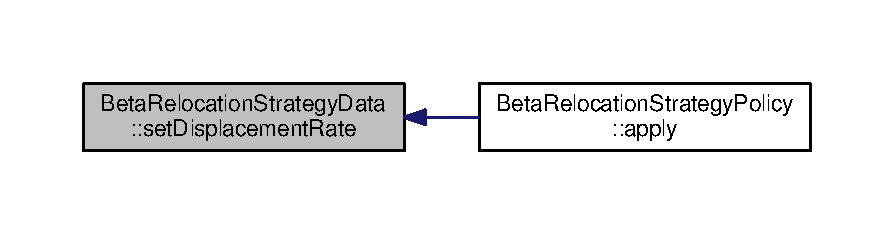
\includegraphics[width=350pt]{structBetaRelocationStrategyData_a542d95263cbcd95c32b43f31881331a5_icgraph}
\end{center}
\end{figure}




\subsection{Field Documentation}
\index{Beta\+Relocation\+Strategy\+Data@{Beta\+Relocation\+Strategy\+Data}!beta\+Acceleration\+Coef@{beta\+Acceleration\+Coef}}
\index{beta\+Acceleration\+Coef@{beta\+Acceleration\+Coef}!Beta\+Relocation\+Strategy\+Data@{Beta\+Relocation\+Strategy\+Data}}
\subsubsection[{\texorpdfstring{beta\+Acceleration\+Coef}{betaAccelerationCoef}}]{\setlength{\rightskip}{0pt plus 5cm}template$<$class P = double, int p\+Size = 1, class F = double, int f\+Size = 1, class V = double, int v\+Size = 1$>$ double {\bf Beta\+Relocation\+Strategy\+Data}$<$ P, p\+Size, F, f\+Size, V, v\+Size $>$\+::beta\+Acceleration\+Coef}\hypertarget{structBetaRelocationStrategyData_a957ba3439a50f2dadf2e500ac0cfcd3c}{}\label{structBetaRelocationStrategyData_a957ba3439a50f2dadf2e500ac0cfcd3c}


Definition at line 38 of file Beta\+Relocation\+Strategy\+Data.\+h.

\index{Beta\+Relocation\+Strategy\+Data@{Beta\+Relocation\+Strategy\+Data}!beta\+Max@{beta\+Max}}
\index{beta\+Max@{beta\+Max}!Beta\+Relocation\+Strategy\+Data@{Beta\+Relocation\+Strategy\+Data}}
\subsubsection[{\texorpdfstring{beta\+Max}{betaMax}}]{\setlength{\rightskip}{0pt plus 5cm}template$<$class P = double, int p\+Size = 1, class F = double, int f\+Size = 1, class V = double, int v\+Size = 1$>$ double {\bf Beta\+Relocation\+Strategy\+Data}$<$ P, p\+Size, F, f\+Size, V, v\+Size $>$\+::beta\+Max}\hypertarget{structBetaRelocationStrategyData_acfd06a41587b792b0f85807fe800b46a}{}\label{structBetaRelocationStrategyData_acfd06a41587b792b0f85807fe800b46a}


Definition at line 36 of file Beta\+Relocation\+Strategy\+Data.\+h.

\index{Beta\+Relocation\+Strategy\+Data@{Beta\+Relocation\+Strategy\+Data}!beta\+Starting\+Perc@{beta\+Starting\+Perc}}
\index{beta\+Starting\+Perc@{beta\+Starting\+Perc}!Beta\+Relocation\+Strategy\+Data@{Beta\+Relocation\+Strategy\+Data}}
\subsubsection[{\texorpdfstring{beta\+Starting\+Perc}{betaStartingPerc}}]{\setlength{\rightskip}{0pt plus 5cm}template$<$class P = double, int p\+Size = 1, class F = double, int f\+Size = 1, class V = double, int v\+Size = 1$>$ double {\bf Beta\+Relocation\+Strategy\+Data}$<$ P, p\+Size, F, f\+Size, V, v\+Size $>$\+::beta\+Starting\+Perc}\hypertarget{structBetaRelocationStrategyData_a979c9c710b41d2d745ef519b4eff2b9b}{}\label{structBetaRelocationStrategyData_a979c9c710b41d2d745ef519b4eff2b9b}


Definition at line 35 of file Beta\+Relocation\+Strategy\+Data.\+h.

\index{Beta\+Relocation\+Strategy\+Data@{Beta\+Relocation\+Strategy\+Data}!displacement\+Rate@{displacement\+Rate}}
\index{displacement\+Rate@{displacement\+Rate}!Beta\+Relocation\+Strategy\+Data@{Beta\+Relocation\+Strategy\+Data}}
\subsubsection[{\texorpdfstring{displacement\+Rate}{displacementRate}}]{\setlength{\rightskip}{0pt plus 5cm}template$<$class P = double, int p\+Size = 1, class F = double, int f\+Size = 1, class V = double, int v\+Size = 1$>$ double {\bf Beta\+Relocation\+Strategy\+Data}$<$ P, p\+Size, F, f\+Size, V, v\+Size $>$\+::displacement\+Rate}\hypertarget{structBetaRelocationStrategyData_a92704a1adaddfe1d7545fd3f1c921fcd}{}\label{structBetaRelocationStrategyData_a92704a1adaddfe1d7545fd3f1c921fcd}


Definition at line 37 of file Beta\+Relocation\+Strategy\+Data.\+h.



The documentation for this class was generated from the following file\+:\begin{DoxyCompactItemize}
\item 
src/\+T\+H/\hyperlink{BetaRelocationStrategyData_8h}{Beta\+Relocation\+Strategy\+Data.\+h}\end{DoxyCompactItemize}

\hypertarget{classBetaRelocationStrategyPolicy}{}\section{Beta\+Relocation\+Strategy\+Policy$<$ P, p\+Size, F, f\+Size, V, v\+Size $>$ Class Template Reference}
\label{classBetaRelocationStrategyPolicy}\index{Beta\+Relocation\+Strategy\+Policy$<$ P, p\+Size, F, f\+Size, V, v\+Size $>$@{Beta\+Relocation\+Strategy\+Policy$<$ P, p\+Size, F, f\+Size, V, v\+Size $>$}}


This policy relocates the population based on the Beta-\/distribution strategy.  




{\ttfamily \#include $<$Beta\+Relocation\+Strategy\+Policy.\+h$>$}



Inheritance diagram for Beta\+Relocation\+Strategy\+Policy$<$ P, p\+Size, F, f\+Size, V, v\+Size $>$\+:
\nopagebreak
\begin{figure}[H]
\begin{center}
\leavevmode
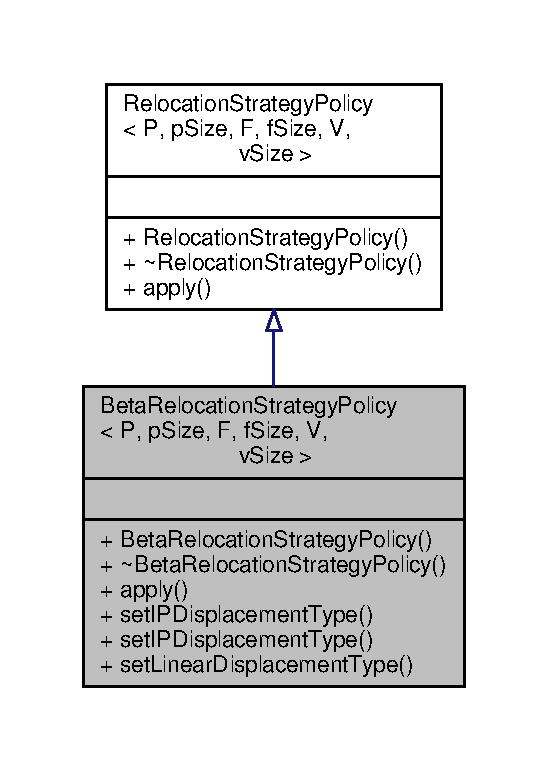
\includegraphics[width=263pt]{classBetaRelocationStrategyPolicy__inherit__graph}
\end{center}
\end{figure}


Collaboration diagram for Beta\+Relocation\+Strategy\+Policy$<$ P, p\+Size, F, f\+Size, V, v\+Size $>$\+:
\nopagebreak
\begin{figure}[H]
\begin{center}
\leavevmode
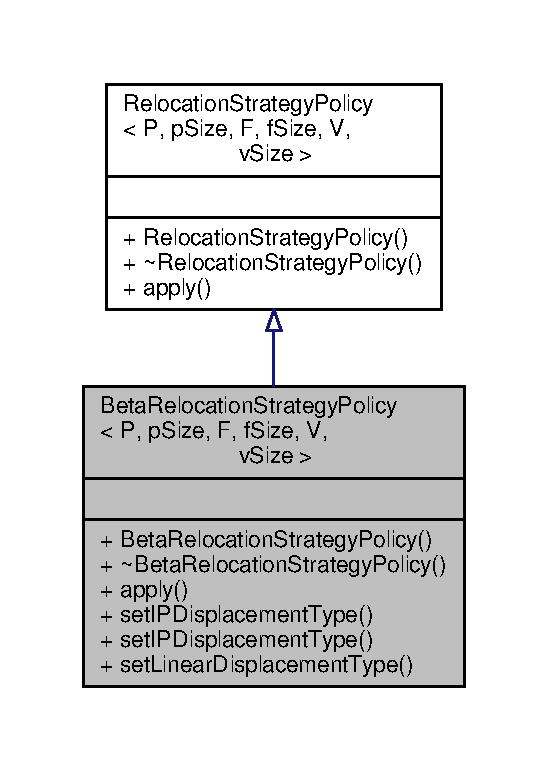
\includegraphics[width=263pt]{classBetaRelocationStrategyPolicy__coll__graph}
\end{center}
\end{figure}
\subsection*{Public Member Functions}
\begin{DoxyCompactItemize}
\item 
\hyperlink{classBetaRelocationStrategyPolicy_a3787cd91ed77d150601350420ca218a6}{Beta\+Relocation\+Strategy\+Policy} ()
\item 
\hyperlink{classBetaRelocationStrategyPolicy_aeaae2cffc71441309bfd6a3e85ad20b1}{$\sim$\+Beta\+Relocation\+Strategy\+Policy} ()
\item 
void \hyperlink{classBetaRelocationStrategyPolicy_aeadaa254d012725ab1a67419d9cb37ef}{apply} (\hyperlink{structRelocationStrategyData}{Relocation\+Strategy\+Data}$<$ P, p\+Size, F, f\+Size, V, v\+Size $>$ $\ast$relocation\+Strategy\+Data, \hyperlink{classRegion}{Region}$<$ P $>$ $\ast$region, \hyperlink{classSolution}{Solution}$<$ P, p\+Size, F, f\+Size, V, v\+Size $>$ $\ast$$\ast$population, int population\+Size)
\begin{DoxyCompactList}\small\item\em This method implements the policy to relocate \hyperlink{classTH}{TH} instance\textquotesingle{}s population at every \hyperlink{classTH}{TH} instance\textquotesingle{}s iteration, based on the Beta-\/distribution strategy. \end{DoxyCompactList}\item 
void \hyperlink{classBetaRelocationStrategyPolicy_a12eb75cb0893c1e1e7795649daa44fdc}{set\+I\+P\+Displacement\+Type} ()
\item 
void \hyperlink{classBetaRelocationStrategyPolicy_aaf793d5a18e2ae159254e7f41b005a6e}{set\+I\+P\+Displacement\+Type} (char boost\+Type, double boost\+Inc, int n\+Tries)
\item 
void \hyperlink{classBetaRelocationStrategyPolicy_ae787cff433b5ce2b6ee8c37b11d6fbfb}{set\+Linear\+Displacement\+Type} ()
\end{DoxyCompactItemize}


\subsection{Detailed Description}
\subsubsection*{template$<$class P = double, int p\+Size = 1, class F = double, int f\+Size = 1, class V = double, int v\+Size = 1$>$\\*
class Beta\+Relocation\+Strategy\+Policy$<$ P, p\+Size, F, f\+Size, V, v\+Size $>$}

This policy relocates the population based on the Beta-\/distribution strategy. 

\begin{DoxyAuthor}{Author}
Peter Frank Perroni 
\end{DoxyAuthor}
\begin{DoxyNote}{Note}
For the Iterative Partitioning method used, please refer (and cite) to the following paper\+:~\newline
 {\itshape P\+E\+R\+R\+O\+NI, Peter Frank; W\+E\+I\+N\+G\+A\+E\+R\+T\+N\+ER, Daniel; D\+E\+L\+G\+A\+DO, Myriam Regattieri. Automated iterative partitioning for cooperatively coevolving particle swarms in large scale optimization. In\+: 2015 Brazilian Conference on Intelligent Systems (B\+R\+A\+C\+IS). I\+E\+EE, 2015. p. 19-\/24.} 
\end{DoxyNote}


Definition at line 49 of file Beta\+Relocation\+Strategy\+Policy.\+h.



\subsection{Constructor \& Destructor Documentation}
\index{Beta\+Relocation\+Strategy\+Policy@{Beta\+Relocation\+Strategy\+Policy}!Beta\+Relocation\+Strategy\+Policy@{Beta\+Relocation\+Strategy\+Policy}}
\index{Beta\+Relocation\+Strategy\+Policy@{Beta\+Relocation\+Strategy\+Policy}!Beta\+Relocation\+Strategy\+Policy@{Beta\+Relocation\+Strategy\+Policy}}
\subsubsection[{\texorpdfstring{Beta\+Relocation\+Strategy\+Policy()}{BetaRelocationStrategyPolicy()}}]{\setlength{\rightskip}{0pt plus 5cm}template$<$class P = double, int p\+Size = 1, class F = double, int f\+Size = 1, class V = double, int v\+Size = 1$>$ {\bf Beta\+Relocation\+Strategy\+Policy}$<$ P, p\+Size, F, f\+Size, V, v\+Size $>$\+::{\bf Beta\+Relocation\+Strategy\+Policy} (
\begin{DoxyParamCaption}
{}
\end{DoxyParamCaption}
)\hspace{0.3cm}{\ttfamily [inline]}}\hypertarget{classBetaRelocationStrategyPolicy_a3787cd91ed77d150601350420ca218a6}{}\label{classBetaRelocationStrategyPolicy_a3787cd91ed77d150601350420ca218a6}


Definition at line 96 of file Beta\+Relocation\+Strategy\+Policy.\+h.



Here is the call graph for this function\+:
\nopagebreak
\begin{figure}[H]
\begin{center}
\leavevmode
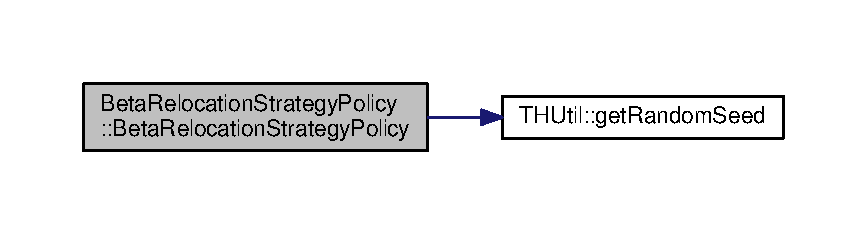
\includegraphics[width=350pt]{classBetaRelocationStrategyPolicy_a3787cd91ed77d150601350420ca218a6_cgraph}
\end{center}
\end{figure}


\index{Beta\+Relocation\+Strategy\+Policy@{Beta\+Relocation\+Strategy\+Policy}!````~Beta\+Relocation\+Strategy\+Policy@{$\sim$\+Beta\+Relocation\+Strategy\+Policy}}
\index{````~Beta\+Relocation\+Strategy\+Policy@{$\sim$\+Beta\+Relocation\+Strategy\+Policy}!Beta\+Relocation\+Strategy\+Policy@{Beta\+Relocation\+Strategy\+Policy}}
\subsubsection[{\texorpdfstring{$\sim$\+Beta\+Relocation\+Strategy\+Policy()}{~BetaRelocationStrategyPolicy()}}]{\setlength{\rightskip}{0pt plus 5cm}template$<$class P = double, int p\+Size = 1, class F = double, int f\+Size = 1, class V = double, int v\+Size = 1$>$ {\bf Beta\+Relocation\+Strategy\+Policy}$<$ P, p\+Size, F, f\+Size, V, v\+Size $>$\+::$\sim${\bf Beta\+Relocation\+Strategy\+Policy} (
\begin{DoxyParamCaption}
{}
\end{DoxyParamCaption}
)\hspace{0.3cm}{\ttfamily [inline]}}\hypertarget{classBetaRelocationStrategyPolicy_aeaae2cffc71441309bfd6a3e85ad20b1}{}\label{classBetaRelocationStrategyPolicy_aeaae2cffc71441309bfd6a3e85ad20b1}


Definition at line 106 of file Beta\+Relocation\+Strategy\+Policy.\+h.



\subsection{Member Function Documentation}
\index{Beta\+Relocation\+Strategy\+Policy@{Beta\+Relocation\+Strategy\+Policy}!apply@{apply}}
\index{apply@{apply}!Beta\+Relocation\+Strategy\+Policy@{Beta\+Relocation\+Strategy\+Policy}}
\subsubsection[{\texorpdfstring{apply(\+Relocation\+Strategy\+Data$<$ P, p\+Size, F, f\+Size, V, v\+Size $>$ $\ast$relocation\+Strategy\+Data, Region$<$ P $>$ $\ast$region, Solution$<$ P, p\+Size, F, f\+Size, V, v\+Size $>$ $\ast$$\ast$population, int population\+Size)}{apply(RelocationStrategyData< P, pSize, F, fSize, V, vSize > *relocationStrategyData, Region< P > *region, Solution< P, pSize, F, fSize, V, vSize > **population, int populationSize)}}]{\setlength{\rightskip}{0pt plus 5cm}template$<$class P = double, int p\+Size = 1, class F = double, int f\+Size = 1, class V = double, int v\+Size = 1$>$ void {\bf Beta\+Relocation\+Strategy\+Policy}$<$ P, p\+Size, F, f\+Size, V, v\+Size $>$\+::apply (
\begin{DoxyParamCaption}
\item[{{\bf Relocation\+Strategy\+Data}$<$ P, p\+Size, F, f\+Size, V, v\+Size $>$ $\ast$}]{relocation\+Strategy\+Data, }
\item[{{\bf Region}$<$ P $>$ $\ast$}]{region, }
\item[{{\bf Solution}$<$ P, p\+Size, F, f\+Size, V, v\+Size $>$ $\ast$$\ast$}]{population, }
\item[{int}]{population\+Size}
\end{DoxyParamCaption}
)\hspace{0.3cm}{\ttfamily [inline]}, {\ttfamily [virtual]}}\hypertarget{classBetaRelocationStrategyPolicy_aeadaa254d012725ab1a67419d9cb37ef}{}\label{classBetaRelocationStrategyPolicy_aeadaa254d012725ab1a67419d9cb37ef}


This method implements the policy to relocate \hyperlink{classTH}{TH} instance\textquotesingle{}s population at every \hyperlink{classTH}{TH} instance\textquotesingle{}s iteration, based on the Beta-\/distribution strategy. 


\begin{DoxyParams}{Parameters}
{\em relocation\+Strategy\+Data} & The repository containing useful data to perform the relocation. \\
\hline
{\em region} & The \char`\"{}anchor\char`\"{} \hyperlink{classRegion}{Region} for current \hyperlink{classTH}{TH} instance. \\
\hline
{\em population} & The population, which is comprised of a list of solutions. \\
\hline
{\em population\+Size} & The population size. \\
\hline
\end{DoxyParams}


Implements \hyperlink{classRelocationStrategyPolicy_ab1de627ca81a24739d942806cfed27e0}{Relocation\+Strategy\+Policy$<$ P, p\+Size, F, f\+Size, V, v\+Size $>$}.



Definition at line 117 of file Beta\+Relocation\+Strategy\+Policy.\+h.



Here is the call graph for this function\+:
\nopagebreak
\begin{figure}[H]
\begin{center}
\leavevmode
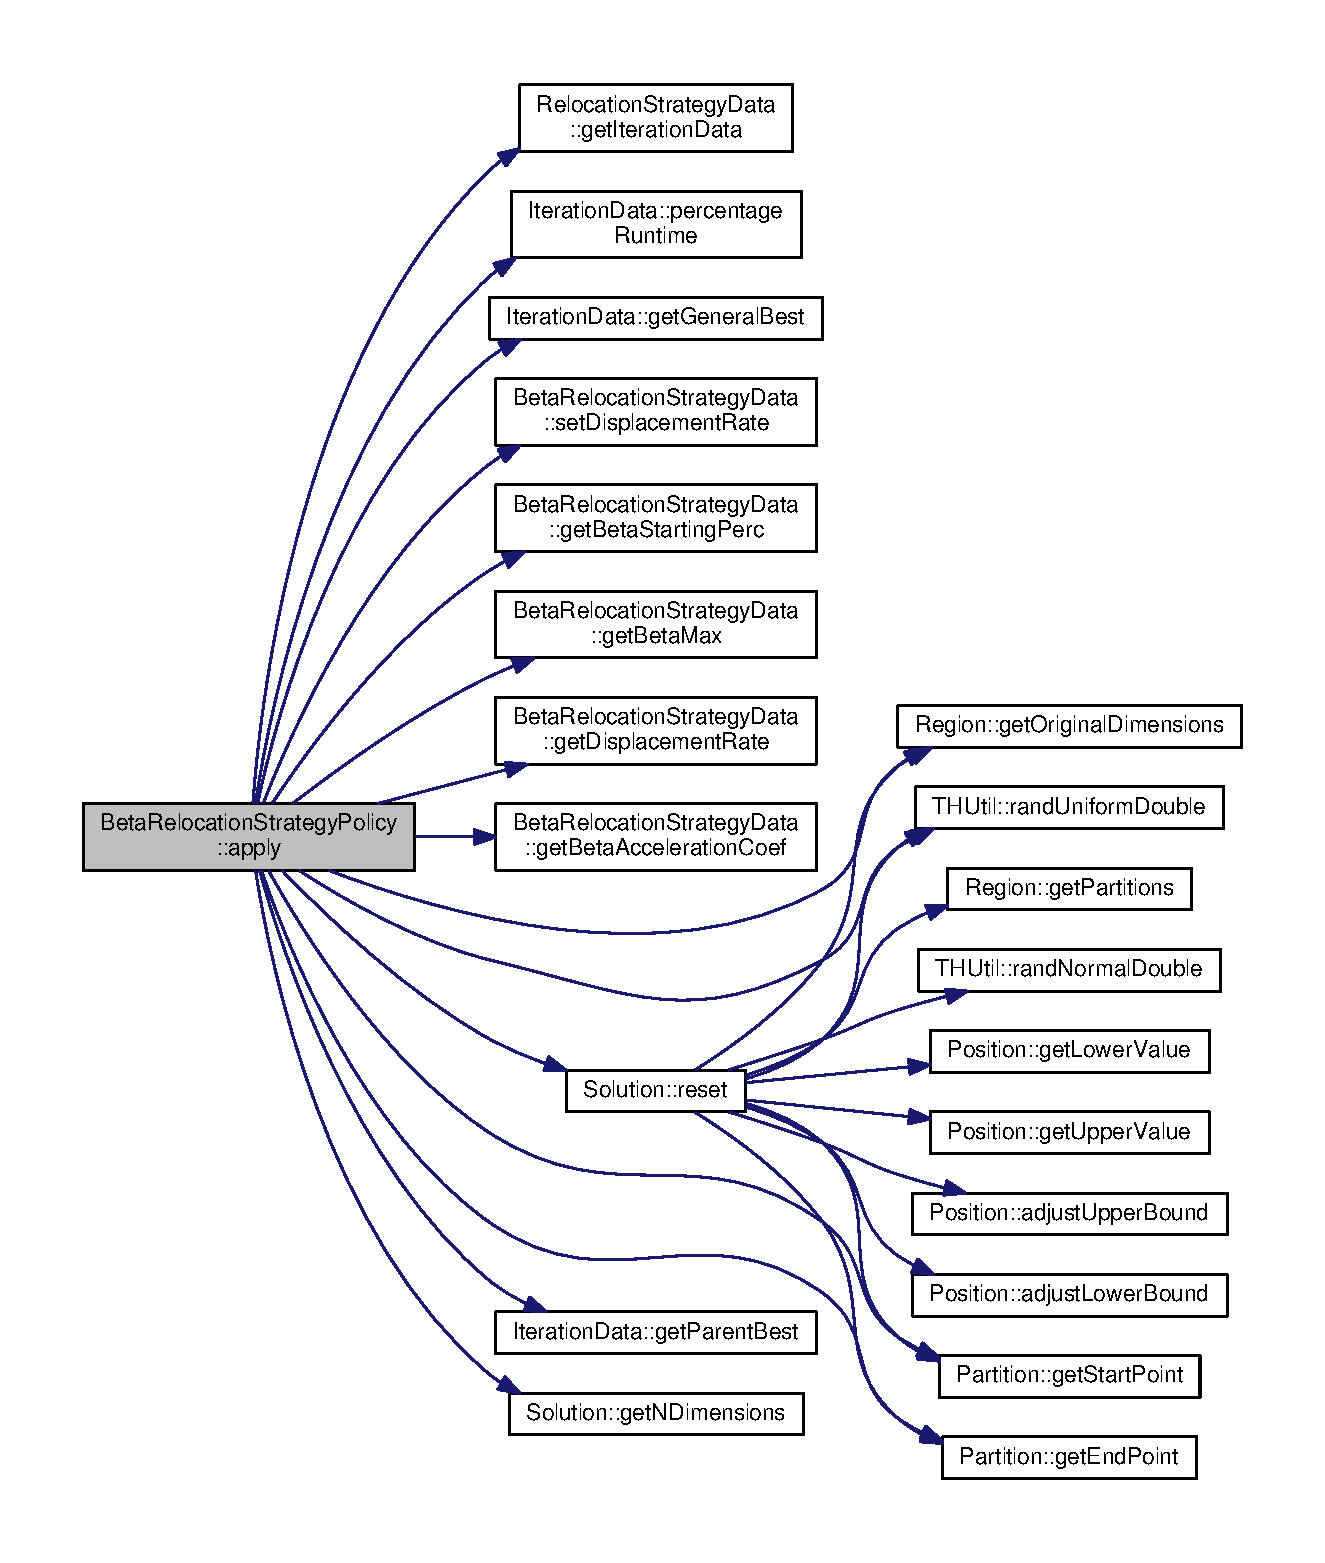
\includegraphics[width=350pt]{classBetaRelocationStrategyPolicy_aeadaa254d012725ab1a67419d9cb37ef_cgraph}
\end{center}
\end{figure}


\index{Beta\+Relocation\+Strategy\+Policy@{Beta\+Relocation\+Strategy\+Policy}!set\+I\+P\+Displacement\+Type@{set\+I\+P\+Displacement\+Type}}
\index{set\+I\+P\+Displacement\+Type@{set\+I\+P\+Displacement\+Type}!Beta\+Relocation\+Strategy\+Policy@{Beta\+Relocation\+Strategy\+Policy}}
\subsubsection[{\texorpdfstring{set\+I\+P\+Displacement\+Type()}{setIPDisplacementType()}}]{\setlength{\rightskip}{0pt plus 5cm}template$<$class P = double, int p\+Size = 1, class F = double, int f\+Size = 1, class V = double, int v\+Size = 1$>$ void {\bf Beta\+Relocation\+Strategy\+Policy}$<$ P, p\+Size, F, f\+Size, V, v\+Size $>$\+::set\+I\+P\+Displacement\+Type (
\begin{DoxyParamCaption}
{}
\end{DoxyParamCaption}
)\hspace{0.3cm}{\ttfamily [inline]}}\hypertarget{classBetaRelocationStrategyPolicy_a12eb75cb0893c1e1e7795649daa44fdc}{}\label{classBetaRelocationStrategyPolicy_a12eb75cb0893c1e1e7795649daa44fdc}


Definition at line 170 of file Beta\+Relocation\+Strategy\+Policy.\+h.

\index{Beta\+Relocation\+Strategy\+Policy@{Beta\+Relocation\+Strategy\+Policy}!set\+I\+P\+Displacement\+Type@{set\+I\+P\+Displacement\+Type}}
\index{set\+I\+P\+Displacement\+Type@{set\+I\+P\+Displacement\+Type}!Beta\+Relocation\+Strategy\+Policy@{Beta\+Relocation\+Strategy\+Policy}}
\subsubsection[{\texorpdfstring{set\+I\+P\+Displacement\+Type(char boost\+Type, double boost\+Inc, int n\+Tries)}{setIPDisplacementType(char boostType, double boostInc, int nTries)}}]{\setlength{\rightskip}{0pt plus 5cm}template$<$class P = double, int p\+Size = 1, class F = double, int f\+Size = 1, class V = double, int v\+Size = 1$>$ void {\bf Beta\+Relocation\+Strategy\+Policy}$<$ P, p\+Size, F, f\+Size, V, v\+Size $>$\+::set\+I\+P\+Displacement\+Type (
\begin{DoxyParamCaption}
\item[{char}]{boost\+Type, }
\item[{double}]{boost\+Inc, }
\item[{int}]{n\+Tries}
\end{DoxyParamCaption}
)\hspace{0.3cm}{\ttfamily [inline]}}\hypertarget{classBetaRelocationStrategyPolicy_aaf793d5a18e2ae159254e7f41b005a6e}{}\label{classBetaRelocationStrategyPolicy_aaf793d5a18e2ae159254e7f41b005a6e}


Definition at line 175 of file Beta\+Relocation\+Strategy\+Policy.\+h.

\index{Beta\+Relocation\+Strategy\+Policy@{Beta\+Relocation\+Strategy\+Policy}!set\+Linear\+Displacement\+Type@{set\+Linear\+Displacement\+Type}}
\index{set\+Linear\+Displacement\+Type@{set\+Linear\+Displacement\+Type}!Beta\+Relocation\+Strategy\+Policy@{Beta\+Relocation\+Strategy\+Policy}}
\subsubsection[{\texorpdfstring{set\+Linear\+Displacement\+Type()}{setLinearDisplacementType()}}]{\setlength{\rightskip}{0pt plus 5cm}template$<$class P = double, int p\+Size = 1, class F = double, int f\+Size = 1, class V = double, int v\+Size = 1$>$ void {\bf Beta\+Relocation\+Strategy\+Policy}$<$ P, p\+Size, F, f\+Size, V, v\+Size $>$\+::set\+Linear\+Displacement\+Type (
\begin{DoxyParamCaption}
{}
\end{DoxyParamCaption}
)\hspace{0.3cm}{\ttfamily [inline]}}\hypertarget{classBetaRelocationStrategyPolicy_ae787cff433b5ce2b6ee8c37b11d6fbfb}{}\label{classBetaRelocationStrategyPolicy_ae787cff433b5ce2b6ee8c37b11d6fbfb}


Definition at line 182 of file Beta\+Relocation\+Strategy\+Policy.\+h.



The documentation for this class was generated from the following file\+:\begin{DoxyCompactItemize}
\item 
src/\+T\+H/\hyperlink{BetaRelocationStrategyPolicy_8h}{Beta\+Relocation\+Strategy\+Policy.\+h}\end{DoxyCompactItemize}

\hypertarget{structConstraintViolation}{}\section{Constraint\+Violation$<$ V, v\+Size $>$ Class Template Reference}
\label{structConstraintViolation}\index{Constraint\+Violation$<$ V, v\+Size $>$@{Constraint\+Violation$<$ V, v\+Size $>$}}


This structure represents the constraints violated by one \hyperlink{classSolution}{Solution}.  




{\ttfamily \#include $<$Constraint\+Violation.\+h$>$}



Collaboration diagram for Constraint\+Violation$<$ V, v\+Size $>$\+:
\nopagebreak
\begin{figure}[H]
\begin{center}
\leavevmode
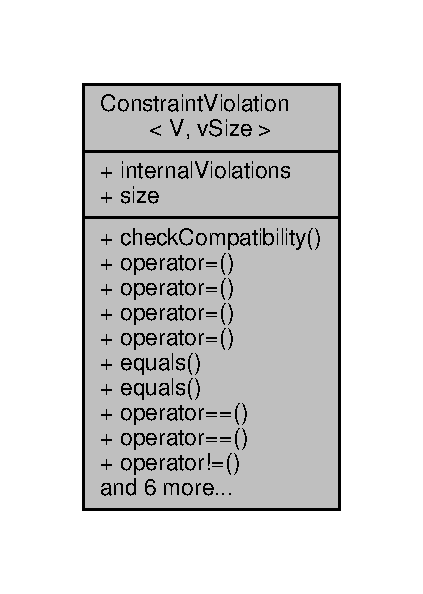
\includegraphics[width=203pt]{structConstraintViolation__coll__graph}
\end{center}
\end{figure}
\subsection*{Public Member Functions}
\begin{DoxyCompactItemize}
\item 
void \hyperlink{structConstraintViolation_a82ebcbfe61ca8adcf6f7b613c4c69f8d}{check\+Compatibility} (\hyperlink{structConstraintViolation}{Constraint\+Violation}$<$ V, v\+Size $>$ $\ast$violation)
\item 
void \hyperlink{structConstraintViolation_a2bfd655f35c83bb9ef8b01102163f519}{operator=} (V $\ast$buffer)
\begin{DoxyCompactList}\small\item\em Operator that assigns the values of a buffer to the list that represents the current \hyperlink{structConstraintViolation}{Constraint\+Violation}. \end{DoxyCompactList}\item 
void \hyperlink{structConstraintViolation_aab52761d8cbde42604d5539d90990876}{operator=} (\hyperlink{structConstraintViolation}{Constraint\+Violation}$<$ V, v\+Size $>$ $\ast$violation)
\begin{DoxyCompactList}\small\item\em Operator that overrides the contents of this list of constraint violations with the contents of the \hyperlink{structConstraintViolation}{Constraint\+Violation} instance received. \end{DoxyCompactList}\item 
void \hyperlink{structConstraintViolation_a303559f871c792bbf9611b64e48918b9}{operator=} (\hyperlink{structConstraintViolation}{Constraint\+Violation}$<$ V, v\+Size $>$ \&violation)
\begin{DoxyCompactList}\small\item\em Operator that overrides the contents of this list of constraint violations with the contents of the \hyperlink{structConstraintViolation}{Constraint\+Violation} instance received. \end{DoxyCompactList}\item 
void \hyperlink{structConstraintViolation_ade5d301bab412f21e9d1e0483af19412}{operator=} (V value)
\begin{DoxyCompactList}\small\item\em Operator that assigns the same value to all elements of the list that represents the current \hyperlink{structConstraintViolation}{Constraint\+Violation}. \end{DoxyCompactList}\item 
bool \hyperlink{structConstraintViolation_a163197175eff749bf4b026c076961120}{equals} (V $\ast$buffer)
\begin{DoxyCompactList}\small\item\em Compares the current list of constraint violations with the buffer received. \end{DoxyCompactList}\item 
bool \hyperlink{structConstraintViolation_ae3f2f69ecc051cde999037c6c7cce276}{equals} (\hyperlink{structConstraintViolation}{Constraint\+Violation}$<$ V, v\+Size $>$ $\ast$violation)
\begin{DoxyCompactList}\small\item\em Compares the current list of constraint violations with the \hyperlink{structConstraintViolation}{Constraint\+Violation} instance received. \end{DoxyCompactList}\item 
bool \hyperlink{structConstraintViolation_a4924e949e9aee8e84cdafea54f2851b9}{operator==} (\hyperlink{structConstraintViolation}{Constraint\+Violation}$<$ V, v\+Size $>$ $\ast$violation)
\item 
bool \hyperlink{structConstraintViolation_aa1e045de24917458b5414675d1473d3d}{operator==} (\hyperlink{structConstraintViolation}{Constraint\+Violation}$<$ V, v\+Size $>$ \&violation)
\item 
bool \hyperlink{structConstraintViolation_abd1a4af7bc87614609e83b69e43732ff}{operator!=} (\hyperlink{structConstraintViolation}{Constraint\+Violation}$<$ V, v\+Size $>$ $\ast$violation)
\item 
bool \hyperlink{structConstraintViolation_a746b126ea8c52c2e8cf479280ba28d56}{operator!=} (\hyperlink{structConstraintViolation}{Constraint\+Violation}$<$ V, v\+Size $>$ \&violation)
\item 
V \hyperlink{structConstraintViolation_a28a71d2bb7a090f92824ae6dadcec646}{get\+Internal\+Violation} (int i)
\begin{DoxyCompactList}\small\item\em Get a constraint violation based on its index in the list of violations. \end{DoxyCompactList}\item 
V $\ast$ \hyperlink{structConstraintViolation_a2cd06f4514a4ebda42d90b3b9b1a6612}{get\+Internal\+Violation} ()
\begin{DoxyCompactList}\small\item\em Get a pointer to the actual list of values that represents the \hyperlink{structConstraintViolation}{Constraint\+Violation}. \end{DoxyCompactList}\item 
void \hyperlink{structConstraintViolation_a78e2b3eb94fc78b767c689e7376228a9}{get\+Internal\+Violation} (V $\ast$buffer)
\begin{DoxyCompactList}\small\item\em This method copies the contents of current \hyperlink{structConstraintViolation}{Constraint\+Violation} to the buffer received. \end{DoxyCompactList}\item 
V \hyperlink{structConstraintViolation_a2d26f6240dd7f4b29f63bd47110fce6b}{get\+First\+Value} ()
\begin{DoxyCompactList}\small\item\em Get the first value from the list of values that represents the \hyperlink{structConstraintViolation}{Constraint\+Violation}. \end{DoxyCompactList}\item 
int \hyperlink{structConstraintViolation_a08e4988745e7389af2f276ead22600ee}{get\+Violation\+Size} ()
\begin{DoxyCompactList}\small\item\em Get the number of values that represents a \hyperlink{structConstraintViolation}{Constraint\+Violation}. \end{DoxyCompactList}\end{DoxyCompactItemize}
\subsection*{Data Fields}
\begin{DoxyCompactItemize}
\item 
V \hyperlink{structConstraintViolation_ac761fb762b35acd21469b3c088be7774}{internal\+Violations} \mbox{[}v\+Size\mbox{]}
\item 
int \hyperlink{structConstraintViolation_a2b1b8e70ce695b7d99cc2b31eb6a0cd9}{size} = v\+Size
\end{DoxyCompactItemize}


\subsection{Detailed Description}
\subsubsection*{template$<$class V = double, int v\+Size = 1$>$\\*
class Constraint\+Violation$<$ V, v\+Size $>$}

This structure represents the constraints violated by one \hyperlink{classSolution}{Solution}. 

\begin{DoxyAuthor}{Author}
Peter Frank Perroni
\end{DoxyAuthor}
The constraint violations are represented by an ordered list with any number of elements, whose type must be of same basic data type for all elements (eg., double or int). 

Definition at line 36 of file Constraint\+Violation.\+h.



\subsection{Member Function Documentation}
\index{Constraint\+Violation@{Constraint\+Violation}!check\+Compatibility@{check\+Compatibility}}
\index{check\+Compatibility@{check\+Compatibility}!Constraint\+Violation@{Constraint\+Violation}}
\subsubsection[{\texorpdfstring{check\+Compatibility(\+Constraint\+Violation$<$ V, v\+Size $>$ $\ast$violation)}{checkCompatibility(ConstraintViolation< V, vSize > *violation)}}]{\setlength{\rightskip}{0pt plus 5cm}template$<$class V = double, int v\+Size = 1$>$ void {\bf Constraint\+Violation}$<$ V, v\+Size $>$\+::check\+Compatibility (
\begin{DoxyParamCaption}
\item[{{\bf Constraint\+Violation}$<$ V, v\+Size $>$ $\ast$}]{violation}
\end{DoxyParamCaption}
)\hspace{0.3cm}{\ttfamily [inline]}}\hypertarget{structConstraintViolation_a82ebcbfe61ca8adcf6f7b613c4c69f8d}{}\label{structConstraintViolation_a82ebcbfe61ca8adcf6f7b613c4c69f8d}


Definition at line 40 of file Constraint\+Violation.\+h.



Here is the caller graph for this function\+:
\nopagebreak
\begin{figure}[H]
\begin{center}
\leavevmode
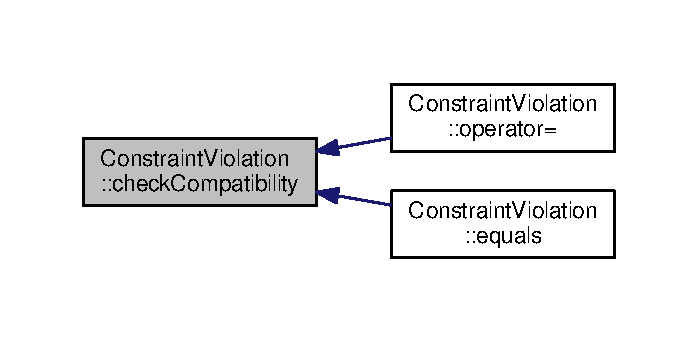
\includegraphics[width=335pt]{structConstraintViolation_a82ebcbfe61ca8adcf6f7b613c4c69f8d_icgraph}
\end{center}
\end{figure}


\index{Constraint\+Violation@{Constraint\+Violation}!equals@{equals}}
\index{equals@{equals}!Constraint\+Violation@{Constraint\+Violation}}
\subsubsection[{\texorpdfstring{equals(\+V $\ast$buffer)}{equals(V *buffer)}}]{\setlength{\rightskip}{0pt plus 5cm}template$<$class V = double, int v\+Size = 1$>$ bool {\bf Constraint\+Violation}$<$ V, v\+Size $>$\+::equals (
\begin{DoxyParamCaption}
\item[{V $\ast$}]{buffer}
\end{DoxyParamCaption}
)\hspace{0.3cm}{\ttfamily [inline]}}\hypertarget{structConstraintViolation_a163197175eff749bf4b026c076961120}{}\label{structConstraintViolation_a163197175eff749bf4b026c076961120}


Compares the current list of constraint violations with the buffer received. 


\begin{DoxyParams}{Parameters}
{\em buffer} & The buffer to compare. \\
\hline
\end{DoxyParams}
\begin{DoxyReturn}{Returns}
True if this \hyperlink{structConstraintViolation}{Constraint\+Violation} instance has the same contents as the buffer received. False otherwise. 
\end{DoxyReturn}


Definition at line 105 of file Constraint\+Violation.\+h.



Here is the caller graph for this function\+:
\nopagebreak
\begin{figure}[H]
\begin{center}
\leavevmode
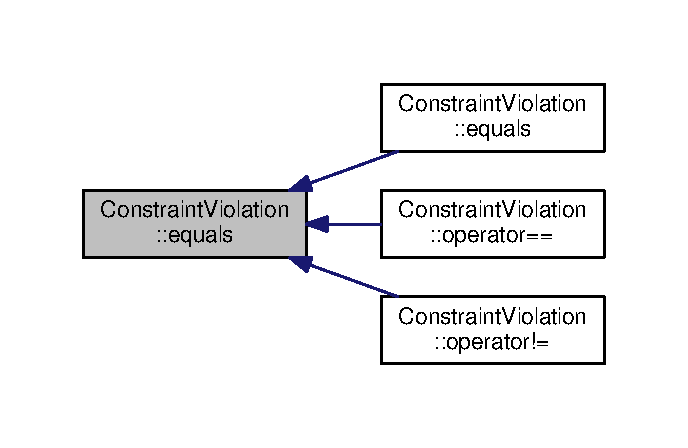
\includegraphics[width=330pt]{structConstraintViolation_a163197175eff749bf4b026c076961120_icgraph}
\end{center}
\end{figure}


\index{Constraint\+Violation@{Constraint\+Violation}!equals@{equals}}
\index{equals@{equals}!Constraint\+Violation@{Constraint\+Violation}}
\subsubsection[{\texorpdfstring{equals(\+Constraint\+Violation$<$ V, v\+Size $>$ $\ast$violation)}{equals(ConstraintViolation< V, vSize > *violation)}}]{\setlength{\rightskip}{0pt plus 5cm}template$<$class V = double, int v\+Size = 1$>$ bool {\bf Constraint\+Violation}$<$ V, v\+Size $>$\+::equals (
\begin{DoxyParamCaption}
\item[{{\bf Constraint\+Violation}$<$ V, v\+Size $>$ $\ast$}]{violation}
\end{DoxyParamCaption}
)\hspace{0.3cm}{\ttfamily [inline]}}\hypertarget{structConstraintViolation_ae3f2f69ecc051cde999037c6c7cce276}{}\label{structConstraintViolation_ae3f2f69ecc051cde999037c6c7cce276}


Compares the current list of constraint violations with the \hyperlink{structConstraintViolation}{Constraint\+Violation} instance received. 


\begin{DoxyParams}{Parameters}
{\em violation} & The \hyperlink{structConstraintViolation}{Constraint\+Violation} instance to compare. \\
\hline
\end{DoxyParams}
\begin{DoxyReturn}{Returns}
True if this \hyperlink{structConstraintViolation}{Constraint\+Violation} instance has the same contents as the one received. False otherwise. 
\end{DoxyReturn}

\begin{DoxyExceptions}{Exceptions}
{\em invalid\+\_\+argument} & if the \hyperlink{structConstraintViolation}{Constraint\+Violation} instance received is not compatible with current list of constraint violations. \\
\hline
\end{DoxyExceptions}


Definition at line 122 of file Constraint\+Violation.\+h.



Here is the call graph for this function\+:
\nopagebreak
\begin{figure}[H]
\begin{center}
\leavevmode
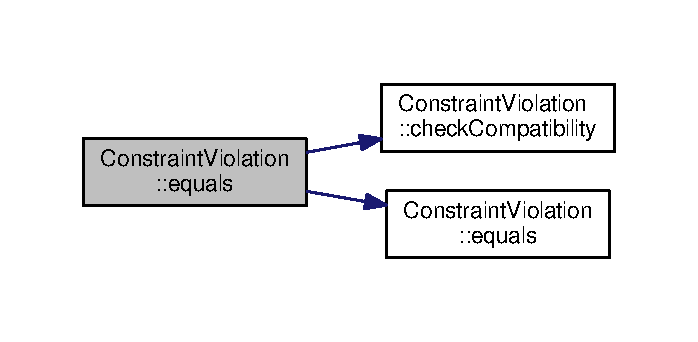
\includegraphics[width=335pt]{structConstraintViolation_ae3f2f69ecc051cde999037c6c7cce276_cgraph}
\end{center}
\end{figure}


\index{Constraint\+Violation@{Constraint\+Violation}!get\+First\+Value@{get\+First\+Value}}
\index{get\+First\+Value@{get\+First\+Value}!Constraint\+Violation@{Constraint\+Violation}}
\subsubsection[{\texorpdfstring{get\+First\+Value()}{getFirstValue()}}]{\setlength{\rightskip}{0pt plus 5cm}template$<$class V = double, int v\+Size = 1$>$ V {\bf Constraint\+Violation}$<$ V, v\+Size $>$\+::get\+First\+Value (
\begin{DoxyParamCaption}
{}
\end{DoxyParamCaption}
)\hspace{0.3cm}{\ttfamily [inline]}}\hypertarget{structConstraintViolation_a2d26f6240dd7f4b29f63bd47110fce6b}{}\label{structConstraintViolation_a2d26f6240dd7f4b29f63bd47110fce6b}


Get the first value from the list of values that represents the \hyperlink{structConstraintViolation}{Constraint\+Violation}. 

Useful when the problem has only a single constraint.

\begin{DoxyReturn}{Returns}
The first value from the list of values that represents the constraint violations. 
\end{DoxyReturn}


Definition at line 175 of file Constraint\+Violation.\+h.

\index{Constraint\+Violation@{Constraint\+Violation}!get\+Internal\+Violation@{get\+Internal\+Violation}}
\index{get\+Internal\+Violation@{get\+Internal\+Violation}!Constraint\+Violation@{Constraint\+Violation}}
\subsubsection[{\texorpdfstring{get\+Internal\+Violation(int i)}{getInternalViolation(int i)}}]{\setlength{\rightskip}{0pt plus 5cm}template$<$class V = double, int v\+Size = 1$>$ V {\bf Constraint\+Violation}$<$ V, v\+Size $>$\+::get\+Internal\+Violation (
\begin{DoxyParamCaption}
\item[{int}]{i}
\end{DoxyParamCaption}
)\hspace{0.3cm}{\ttfamily [inline]}}\hypertarget{structConstraintViolation_a28a71d2bb7a090f92824ae6dadcec646}{}\label{structConstraintViolation_a28a71d2bb7a090f92824ae6dadcec646}


Get a constraint violation based on its index in the list of violations. 


\begin{DoxyParams}{Parameters}
{\em i} & The index of the constraint violation in the list (index list starts in zero). \\
\hline
\end{DoxyParams}
\begin{DoxyReturn}{Returns}
The constraint violation selected. 
\end{DoxyReturn}


Definition at line 144 of file Constraint\+Violation.\+h.

\index{Constraint\+Violation@{Constraint\+Violation}!get\+Internal\+Violation@{get\+Internal\+Violation}}
\index{get\+Internal\+Violation@{get\+Internal\+Violation}!Constraint\+Violation@{Constraint\+Violation}}
\subsubsection[{\texorpdfstring{get\+Internal\+Violation()}{getInternalViolation()}}]{\setlength{\rightskip}{0pt plus 5cm}template$<$class V = double, int v\+Size = 1$>$ V$\ast$ {\bf Constraint\+Violation}$<$ V, v\+Size $>$\+::get\+Internal\+Violation (
\begin{DoxyParamCaption}
{}
\end{DoxyParamCaption}
)\hspace{0.3cm}{\ttfamily [inline]}}\hypertarget{structConstraintViolation_a2cd06f4514a4ebda42d90b3b9b1a6612}{}\label{structConstraintViolation_a2cd06f4514a4ebda42d90b3b9b1a6612}


Get a pointer to the actual list of values that represents the \hyperlink{structConstraintViolation}{Constraint\+Violation}. 

\begin{DoxyReturn}{Returns}
The pointer to the constraint violation\textquotesingle{}s values. 
\end{DoxyReturn}


Definition at line 153 of file Constraint\+Violation.\+h.

\index{Constraint\+Violation@{Constraint\+Violation}!get\+Internal\+Violation@{get\+Internal\+Violation}}
\index{get\+Internal\+Violation@{get\+Internal\+Violation}!Constraint\+Violation@{Constraint\+Violation}}
\subsubsection[{\texorpdfstring{get\+Internal\+Violation(\+V $\ast$buffer)}{getInternalViolation(V *buffer)}}]{\setlength{\rightskip}{0pt plus 5cm}template$<$class V = double, int v\+Size = 1$>$ void {\bf Constraint\+Violation}$<$ V, v\+Size $>$\+::get\+Internal\+Violation (
\begin{DoxyParamCaption}
\item[{V $\ast$}]{buffer}
\end{DoxyParamCaption}
)\hspace{0.3cm}{\ttfamily [inline]}}\hypertarget{structConstraintViolation_a78e2b3eb94fc78b767c689e7376228a9}{}\label{structConstraintViolation_a78e2b3eb94fc78b767c689e7376228a9}


This method copies the contents of current \hyperlink{structConstraintViolation}{Constraint\+Violation} to the buffer received. 


\begin{DoxyParams}{Parameters}
{\em buffer} & The destination buffer. \\
\hline
\end{DoxyParams}


Definition at line 160 of file Constraint\+Violation.\+h.

\index{Constraint\+Violation@{Constraint\+Violation}!get\+Violation\+Size@{get\+Violation\+Size}}
\index{get\+Violation\+Size@{get\+Violation\+Size}!Constraint\+Violation@{Constraint\+Violation}}
\subsubsection[{\texorpdfstring{get\+Violation\+Size()}{getViolationSize()}}]{\setlength{\rightskip}{0pt plus 5cm}template$<$class V = double, int v\+Size = 1$>$ int {\bf Constraint\+Violation}$<$ V, v\+Size $>$\+::get\+Violation\+Size (
\begin{DoxyParamCaption}
{}
\end{DoxyParamCaption}
)\hspace{0.3cm}{\ttfamily [inline]}}\hypertarget{structConstraintViolation_a08e4988745e7389af2f276ead22600ee}{}\label{structConstraintViolation_a08e4988745e7389af2f276ead22600ee}


Get the number of values that represents a \hyperlink{structConstraintViolation}{Constraint\+Violation}. 

\begin{DoxyReturn}{Returns}
The number of values that represents a \hyperlink{structConstraintViolation}{Constraint\+Violation}. 
\end{DoxyReturn}


Definition at line 181 of file Constraint\+Violation.\+h.

\index{Constraint\+Violation@{Constraint\+Violation}!operator"!=@{operator"!=}}
\index{operator"!=@{operator"!=}!Constraint\+Violation@{Constraint\+Violation}}
\subsubsection[{\texorpdfstring{operator"!=(\+Constraint\+Violation$<$ V, v\+Size $>$ $\ast$violation)}{operator!=(ConstraintViolation< V, vSize > *violation)}}]{\setlength{\rightskip}{0pt plus 5cm}template$<$class V = double, int v\+Size = 1$>$ bool {\bf Constraint\+Violation}$<$ V, v\+Size $>$\+::operator!= (
\begin{DoxyParamCaption}
\item[{{\bf Constraint\+Violation}$<$ V, v\+Size $>$ $\ast$}]{violation}
\end{DoxyParamCaption}
)\hspace{0.3cm}{\ttfamily [inline]}}\hypertarget{structConstraintViolation_abd1a4af7bc87614609e83b69e43732ff}{}\label{structConstraintViolation_abd1a4af7bc87614609e83b69e43732ff}


Definition at line 132 of file Constraint\+Violation.\+h.



Here is the call graph for this function\+:
\nopagebreak
\begin{figure}[H]
\begin{center}
\leavevmode
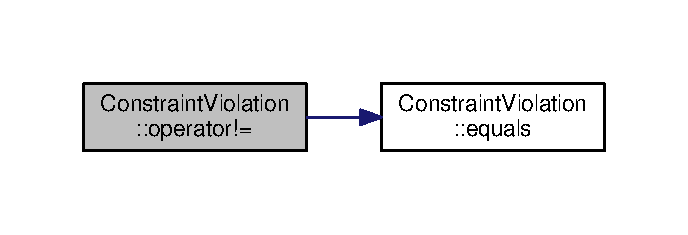
\includegraphics[width=330pt]{structConstraintViolation_abd1a4af7bc87614609e83b69e43732ff_cgraph}
\end{center}
\end{figure}


\index{Constraint\+Violation@{Constraint\+Violation}!operator"!=@{operator"!=}}
\index{operator"!=@{operator"!=}!Constraint\+Violation@{Constraint\+Violation}}
\subsubsection[{\texorpdfstring{operator"!=(\+Constraint\+Violation$<$ V, v\+Size $>$ \&violation)}{operator!=(ConstraintViolation< V, vSize > &violation)}}]{\setlength{\rightskip}{0pt plus 5cm}template$<$class V = double, int v\+Size = 1$>$ bool {\bf Constraint\+Violation}$<$ V, v\+Size $>$\+::operator!= (
\begin{DoxyParamCaption}
\item[{{\bf Constraint\+Violation}$<$ V, v\+Size $>$ \&}]{violation}
\end{DoxyParamCaption}
)\hspace{0.3cm}{\ttfamily [inline]}}\hypertarget{structConstraintViolation_a746b126ea8c52c2e8cf479280ba28d56}{}\label{structConstraintViolation_a746b126ea8c52c2e8cf479280ba28d56}


Definition at line 135 of file Constraint\+Violation.\+h.



Here is the call graph for this function\+:
\nopagebreak
\begin{figure}[H]
\begin{center}
\leavevmode
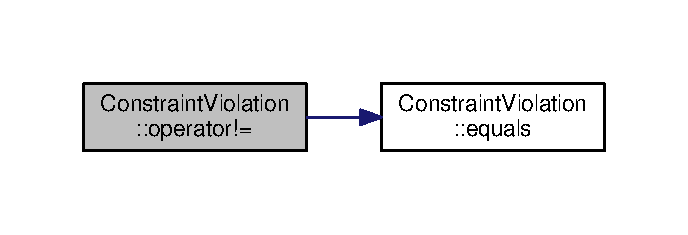
\includegraphics[width=330pt]{structConstraintViolation_a746b126ea8c52c2e8cf479280ba28d56_cgraph}
\end{center}
\end{figure}


\index{Constraint\+Violation@{Constraint\+Violation}!operator=@{operator=}}
\index{operator=@{operator=}!Constraint\+Violation@{Constraint\+Violation}}
\subsubsection[{\texorpdfstring{operator=(\+V $\ast$buffer)}{operator=(V *buffer)}}]{\setlength{\rightskip}{0pt plus 5cm}template$<$class V = double, int v\+Size = 1$>$ void {\bf Constraint\+Violation}$<$ V, v\+Size $>$\+::operator= (
\begin{DoxyParamCaption}
\item[{V $\ast$}]{buffer}
\end{DoxyParamCaption}
)\hspace{0.3cm}{\ttfamily [inline]}}\hypertarget{structConstraintViolation_a2bfd655f35c83bb9ef8b01102163f519}{}\label{structConstraintViolation_a2bfd655f35c83bb9ef8b01102163f519}


Operator that assigns the values of a buffer to the list that represents the current \hyperlink{structConstraintViolation}{Constraint\+Violation}. 


\begin{DoxyParams}{Parameters}
{\em buffer} & The source buffer to assign to the list. \\
\hline
\end{DoxyParams}


Definition at line 55 of file Constraint\+Violation.\+h.

\index{Constraint\+Violation@{Constraint\+Violation}!operator=@{operator=}}
\index{operator=@{operator=}!Constraint\+Violation@{Constraint\+Violation}}
\subsubsection[{\texorpdfstring{operator=(\+Constraint\+Violation$<$ V, v\+Size $>$ $\ast$violation)}{operator=(ConstraintViolation< V, vSize > *violation)}}]{\setlength{\rightskip}{0pt plus 5cm}template$<$class V = double, int v\+Size = 1$>$ void {\bf Constraint\+Violation}$<$ V, v\+Size $>$\+::operator= (
\begin{DoxyParamCaption}
\item[{{\bf Constraint\+Violation}$<$ V, v\+Size $>$ $\ast$}]{violation}
\end{DoxyParamCaption}
)\hspace{0.3cm}{\ttfamily [inline]}}\hypertarget{structConstraintViolation_aab52761d8cbde42604d5539d90990876}{}\label{structConstraintViolation_aab52761d8cbde42604d5539d90990876}


Operator that overrides the contents of this list of constraint violations with the contents of the \hyperlink{structConstraintViolation}{Constraint\+Violation} instance received. 


\begin{DoxyParams}{Parameters}
{\em fitness} & The source \hyperlink{structConstraintViolation}{Constraint\+Violation} instance. \\
\hline
\end{DoxyParams}

\begin{DoxyExceptions}{Exceptions}
{\em invalid\+\_\+argument} & if the source \hyperlink{structConstraintViolation}{Constraint\+Violation} instance is not compatible with current \hyperlink{structConstraintViolation}{Constraint\+Violation} instance. \\
\hline
\end{DoxyExceptions}


Definition at line 70 of file Constraint\+Violation.\+h.



Here is the call graph for this function\+:
\nopagebreak
\begin{figure}[H]
\begin{center}
\leavevmode
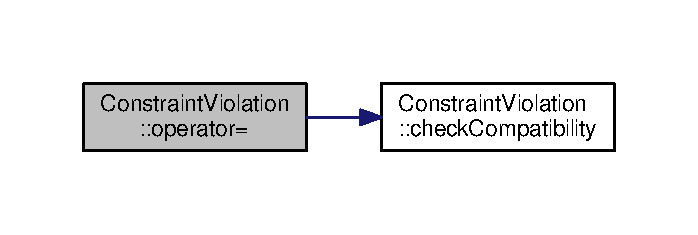
\includegraphics[width=335pt]{structConstraintViolation_aab52761d8cbde42604d5539d90990876_cgraph}
\end{center}
\end{figure}


\index{Constraint\+Violation@{Constraint\+Violation}!operator=@{operator=}}
\index{operator=@{operator=}!Constraint\+Violation@{Constraint\+Violation}}
\subsubsection[{\texorpdfstring{operator=(\+Constraint\+Violation$<$ V, v\+Size $>$ \&violation)}{operator=(ConstraintViolation< V, vSize > &violation)}}]{\setlength{\rightskip}{0pt plus 5cm}template$<$class V = double, int v\+Size = 1$>$ void {\bf Constraint\+Violation}$<$ V, v\+Size $>$\+::operator= (
\begin{DoxyParamCaption}
\item[{{\bf Constraint\+Violation}$<$ V, v\+Size $>$ \&}]{violation}
\end{DoxyParamCaption}
)\hspace{0.3cm}{\ttfamily [inline]}}\hypertarget{structConstraintViolation_a303559f871c792bbf9611b64e48918b9}{}\label{structConstraintViolation_a303559f871c792bbf9611b64e48918b9}


Operator that overrides the contents of this list of constraint violations with the contents of the \hyperlink{structConstraintViolation}{Constraint\+Violation} instance received. 


\begin{DoxyParams}{Parameters}
{\em fitness} & The source \hyperlink{structConstraintViolation}{Constraint\+Violation} instance. \\
\hline
\end{DoxyParams}

\begin{DoxyExceptions}{Exceptions}
{\em invalid\+\_\+argument} & if the source \hyperlink{structConstraintViolation}{Constraint\+Violation} instance is not compatible with current \hyperlink{structConstraintViolation}{Constraint\+Violation} instance. \\
\hline
\end{DoxyExceptions}


Definition at line 83 of file Constraint\+Violation.\+h.



Here is the call graph for this function\+:
\nopagebreak
\begin{figure}[H]
\begin{center}
\leavevmode
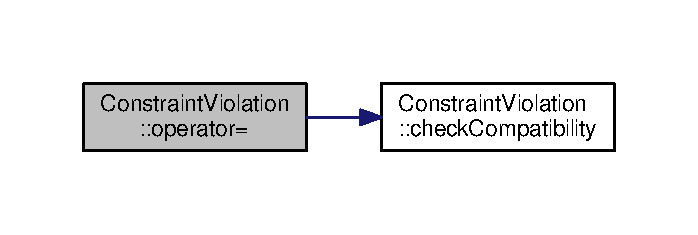
\includegraphics[width=335pt]{structConstraintViolation_a303559f871c792bbf9611b64e48918b9_cgraph}
\end{center}
\end{figure}


\index{Constraint\+Violation@{Constraint\+Violation}!operator=@{operator=}}
\index{operator=@{operator=}!Constraint\+Violation@{Constraint\+Violation}}
\subsubsection[{\texorpdfstring{operator=(\+V value)}{operator=(V value)}}]{\setlength{\rightskip}{0pt plus 5cm}template$<$class V = double, int v\+Size = 1$>$ void {\bf Constraint\+Violation}$<$ V, v\+Size $>$\+::operator= (
\begin{DoxyParamCaption}
\item[{V}]{value}
\end{DoxyParamCaption}
)\hspace{0.3cm}{\ttfamily [inline]}}\hypertarget{structConstraintViolation_ade5d301bab412f21e9d1e0483af19412}{}\label{structConstraintViolation_ade5d301bab412f21e9d1e0483af19412}


Operator that assigns the same value to all elements of the list that represents the current \hyperlink{structConstraintViolation}{Constraint\+Violation}. 


\begin{DoxyParams}{Parameters}
{\em value} & The value to assign to the list. \\
\hline
\end{DoxyParams}


Definition at line 93 of file Constraint\+Violation.\+h.

\index{Constraint\+Violation@{Constraint\+Violation}!operator==@{operator==}}
\index{operator==@{operator==}!Constraint\+Violation@{Constraint\+Violation}}
\subsubsection[{\texorpdfstring{operator==(\+Constraint\+Violation$<$ V, v\+Size $>$ $\ast$violation)}{operator==(ConstraintViolation< V, vSize > *violation)}}]{\setlength{\rightskip}{0pt plus 5cm}template$<$class V = double, int v\+Size = 1$>$ bool {\bf Constraint\+Violation}$<$ V, v\+Size $>$\+::operator== (
\begin{DoxyParamCaption}
\item[{{\bf Constraint\+Violation}$<$ V, v\+Size $>$ $\ast$}]{violation}
\end{DoxyParamCaption}
)\hspace{0.3cm}{\ttfamily [inline]}}\hypertarget{structConstraintViolation_a4924e949e9aee8e84cdafea54f2851b9}{}\label{structConstraintViolation_a4924e949e9aee8e84cdafea54f2851b9}


Definition at line 126 of file Constraint\+Violation.\+h.



Here is the call graph for this function\+:
\nopagebreak
\begin{figure}[H]
\begin{center}
\leavevmode
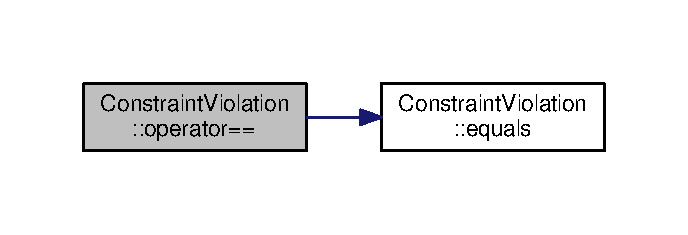
\includegraphics[width=330pt]{structConstraintViolation_a4924e949e9aee8e84cdafea54f2851b9_cgraph}
\end{center}
\end{figure}


\index{Constraint\+Violation@{Constraint\+Violation}!operator==@{operator==}}
\index{operator==@{operator==}!Constraint\+Violation@{Constraint\+Violation}}
\subsubsection[{\texorpdfstring{operator==(\+Constraint\+Violation$<$ V, v\+Size $>$ \&violation)}{operator==(ConstraintViolation< V, vSize > &violation)}}]{\setlength{\rightskip}{0pt plus 5cm}template$<$class V = double, int v\+Size = 1$>$ bool {\bf Constraint\+Violation}$<$ V, v\+Size $>$\+::operator== (
\begin{DoxyParamCaption}
\item[{{\bf Constraint\+Violation}$<$ V, v\+Size $>$ \&}]{violation}
\end{DoxyParamCaption}
)\hspace{0.3cm}{\ttfamily [inline]}}\hypertarget{structConstraintViolation_aa1e045de24917458b5414675d1473d3d}{}\label{structConstraintViolation_aa1e045de24917458b5414675d1473d3d}


Definition at line 129 of file Constraint\+Violation.\+h.



Here is the call graph for this function\+:
\nopagebreak
\begin{figure}[H]
\begin{center}
\leavevmode
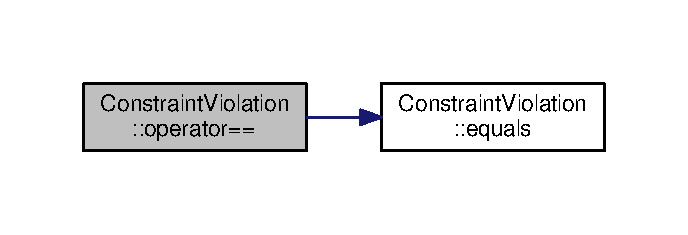
\includegraphics[width=330pt]{structConstraintViolation_aa1e045de24917458b5414675d1473d3d_cgraph}
\end{center}
\end{figure}




\subsection{Field Documentation}
\index{Constraint\+Violation@{Constraint\+Violation}!internal\+Violations@{internal\+Violations}}
\index{internal\+Violations@{internal\+Violations}!Constraint\+Violation@{Constraint\+Violation}}
\subsubsection[{\texorpdfstring{internal\+Violations}{internalViolations}}]{\setlength{\rightskip}{0pt plus 5cm}template$<$class V = double, int v\+Size = 1$>$ V {\bf Constraint\+Violation}$<$ V, v\+Size $>$\+::internal\+Violations\mbox{[}v\+Size\mbox{]}}\hypertarget{structConstraintViolation_ac761fb762b35acd21469b3c088be7774}{}\label{structConstraintViolation_ac761fb762b35acd21469b3c088be7774}


Definition at line 37 of file Constraint\+Violation.\+h.

\index{Constraint\+Violation@{Constraint\+Violation}!size@{size}}
\index{size@{size}!Constraint\+Violation@{Constraint\+Violation}}
\subsubsection[{\texorpdfstring{size}{size}}]{\setlength{\rightskip}{0pt plus 5cm}template$<$class V = double, int v\+Size = 1$>$ int {\bf Constraint\+Violation}$<$ V, v\+Size $>$\+::size = v\+Size}\hypertarget{structConstraintViolation_a2b1b8e70ce695b7d99cc2b31eb6a0cd9}{}\label{structConstraintViolation_a2b1b8e70ce695b7d99cc2b31eb6a0cd9}


Definition at line 38 of file Constraint\+Violation.\+h.



The documentation for this class was generated from the following file\+:\begin{DoxyCompactItemize}
\item 
src/\+T\+H/\hyperlink{ConstraintViolation_8h}{Constraint\+Violation.\+h}\end{DoxyCompactItemize}

\hypertarget{classConvergenceControlPolicy}{}\section{Convergence\+Control\+Policy$<$ P, p\+Size, F, f\+Size, V, v\+Size $>$ Class Template Reference}
\label{classConvergenceControlPolicy}\index{Convergence\+Control\+Policy$<$ P, p\+Size, F, f\+Size, V, v\+Size $>$@{Convergence\+Control\+Policy$<$ P, p\+Size, F, f\+Size, V, v\+Size $>$}}


Template for the policy that runs, monitors and controls the convergence for the current \hyperlink{classTH}{TH} iteration.  




{\ttfamily \#include $<$Convergence\+Control\+Policy.\+h$>$}



Inheritance diagram for Convergence\+Control\+Policy$<$ P, p\+Size, F, f\+Size, V, v\+Size $>$\+:
\nopagebreak
\begin{figure}[H]
\begin{center}
\leavevmode
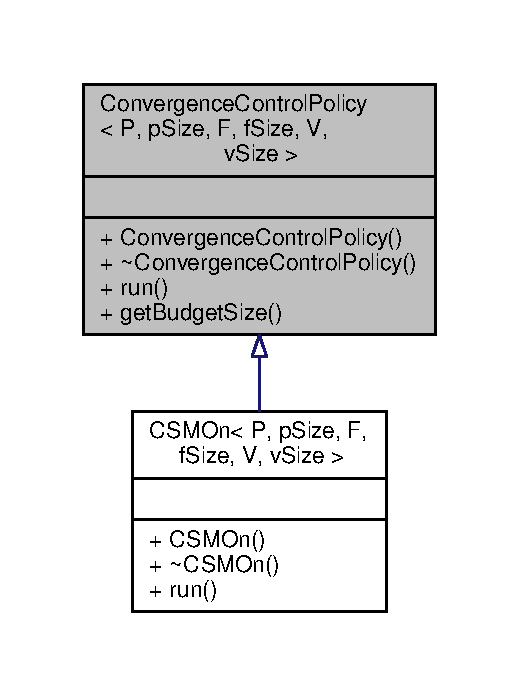
\includegraphics[width=249pt]{classConvergenceControlPolicy__inherit__graph}
\end{center}
\end{figure}


Collaboration diagram for Convergence\+Control\+Policy$<$ P, p\+Size, F, f\+Size, V, v\+Size $>$\+:
\nopagebreak
\begin{figure}[H]
\begin{center}
\leavevmode
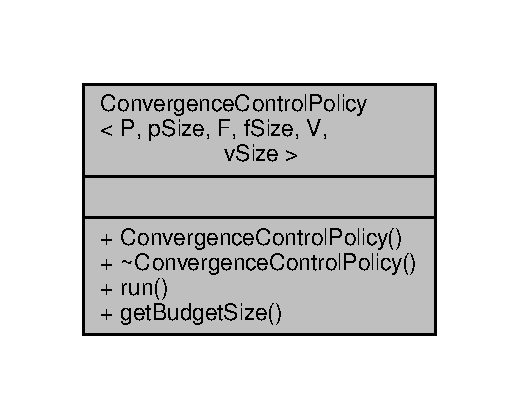
\includegraphics[width=249pt]{classConvergenceControlPolicy__coll__graph}
\end{center}
\end{figure}
\subsection*{Public Member Functions}
\begin{DoxyCompactItemize}
\item 
\hyperlink{classConvergenceControlPolicy_a8882660f0bfd404494339aed74d625a2}{Convergence\+Control\+Policy} (int budget\+Size)
\begin{DoxyCompactList}\small\item\em Constructor to setup the maximum number of fitness function evaluations allowed. \end{DoxyCompactList}\item 
virtual \hyperlink{classConvergenceControlPolicy_a1827a6722494ff97719a2383976e9c11}{$\sim$\+Convergence\+Control\+Policy} ()
\item 
virtual void \hyperlink{classConvergenceControlPolicy_ad72beb5807e87c3fa0602bd0bf4679ac}{run} (\hyperlink{classSearch}{Search}$<$ P, p\+Size, F, f\+Size, V, v\+Size $>$ $\ast$search)=0
\begin{DoxyCompactList}\small\item\em Virtual method that will run, monitor and control one \hyperlink{classTH}{TH} iteration. \end{DoxyCompactList}\item 
int \hyperlink{classConvergenceControlPolicy_a445c537935922b1bcb67d3732abbfe0f}{get\+Budget\+Size} ()
\begin{DoxyCompactList}\small\item\em Get the maximum number of fitness function evaluations allowed. \end{DoxyCompactList}\end{DoxyCompactItemize}


\subsection{Detailed Description}
\subsubsection*{template$<$class P = double, int p\+Size = 1, class F = double, int f\+Size = 1, class V = double, int v\+Size = 1$>$\\*
class Convergence\+Control\+Policy$<$ P, p\+Size, F, f\+Size, V, v\+Size $>$}

Template for the policy that runs, monitors and controls the convergence for the current \hyperlink{classTH}{TH} iteration. 

\begin{DoxyAuthor}{Author}
Peter Frank Perroni 
\end{DoxyAuthor}


Definition at line 34 of file Convergence\+Control\+Policy.\+h.



\subsection{Constructor \& Destructor Documentation}
\index{Convergence\+Control\+Policy@{Convergence\+Control\+Policy}!Convergence\+Control\+Policy@{Convergence\+Control\+Policy}}
\index{Convergence\+Control\+Policy@{Convergence\+Control\+Policy}!Convergence\+Control\+Policy@{Convergence\+Control\+Policy}}
\subsubsection[{\texorpdfstring{Convergence\+Control\+Policy(int budget\+Size)}{ConvergenceControlPolicy(int budgetSize)}}]{\setlength{\rightskip}{0pt plus 5cm}template$<$class P = double, int p\+Size = 1, class F = double, int f\+Size = 1, class V = double, int v\+Size = 1$>$ {\bf Convergence\+Control\+Policy}$<$ P, p\+Size, F, f\+Size, V, v\+Size $>$\+::{\bf Convergence\+Control\+Policy} (
\begin{DoxyParamCaption}
\item[{int}]{budget\+Size}
\end{DoxyParamCaption}
)\hspace{0.3cm}{\ttfamily [inline]}}\hypertarget{classConvergenceControlPolicy_a8882660f0bfd404494339aed74d625a2}{}\label{classConvergenceControlPolicy_a8882660f0bfd404494339aed74d625a2}


Constructor to setup the maximum number of fitness function evaluations allowed. 


\begin{DoxyParams}{Parameters}
{\em budget\+Size} & The maximum number of fitness function evaluations allowed. \\
\hline
\end{DoxyParams}


Definition at line 42 of file Convergence\+Control\+Policy.\+h.

\index{Convergence\+Control\+Policy@{Convergence\+Control\+Policy}!````~Convergence\+Control\+Policy@{$\sim$\+Convergence\+Control\+Policy}}
\index{````~Convergence\+Control\+Policy@{$\sim$\+Convergence\+Control\+Policy}!Convergence\+Control\+Policy@{Convergence\+Control\+Policy}}
\subsubsection[{\texorpdfstring{$\sim$\+Convergence\+Control\+Policy()}{~ConvergenceControlPolicy()}}]{\setlength{\rightskip}{0pt plus 5cm}template$<$class P = double, int p\+Size = 1, class F = double, int f\+Size = 1, class V = double, int v\+Size = 1$>$ virtual {\bf Convergence\+Control\+Policy}$<$ P, p\+Size, F, f\+Size, V, v\+Size $>$\+::$\sim${\bf Convergence\+Control\+Policy} (
\begin{DoxyParamCaption}
{}
\end{DoxyParamCaption}
)\hspace{0.3cm}{\ttfamily [inline]}, {\ttfamily [virtual]}}\hypertarget{classConvergenceControlPolicy_a1827a6722494ff97719a2383976e9c11}{}\label{classConvergenceControlPolicy_a1827a6722494ff97719a2383976e9c11}


Definition at line 45 of file Convergence\+Control\+Policy.\+h.



Here is the call graph for this function\+:
\nopagebreak
\begin{figure}[H]
\begin{center}
\leavevmode
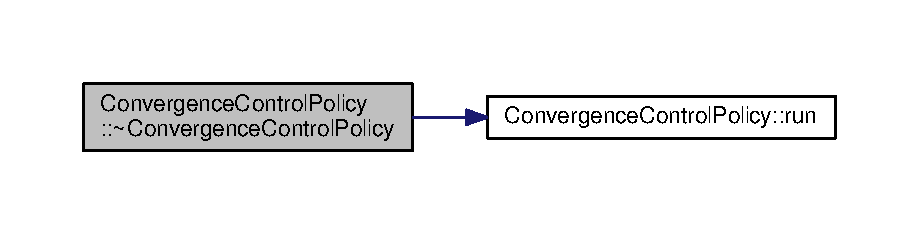
\includegraphics[width=350pt]{classConvergenceControlPolicy_a1827a6722494ff97719a2383976e9c11_cgraph}
\end{center}
\end{figure}




\subsection{Member Function Documentation}
\index{Convergence\+Control\+Policy@{Convergence\+Control\+Policy}!get\+Budget\+Size@{get\+Budget\+Size}}
\index{get\+Budget\+Size@{get\+Budget\+Size}!Convergence\+Control\+Policy@{Convergence\+Control\+Policy}}
\subsubsection[{\texorpdfstring{get\+Budget\+Size()}{getBudgetSize()}}]{\setlength{\rightskip}{0pt plus 5cm}template$<$class P = double, int p\+Size = 1, class F = double, int f\+Size = 1, class V = double, int v\+Size = 1$>$ int {\bf Convergence\+Control\+Policy}$<$ P, p\+Size, F, f\+Size, V, v\+Size $>$\+::get\+Budget\+Size (
\begin{DoxyParamCaption}
{}
\end{DoxyParamCaption}
)\hspace{0.3cm}{\ttfamily [inline]}}\hypertarget{classConvergenceControlPolicy_a445c537935922b1bcb67d3732abbfe0f}{}\label{classConvergenceControlPolicy_a445c537935922b1bcb67d3732abbfe0f}


Get the maximum number of fitness function evaluations allowed. 



Definition at line 61 of file Convergence\+Control\+Policy.\+h.



Here is the caller graph for this function\+:
\nopagebreak
\begin{figure}[H]
\begin{center}
\leavevmode
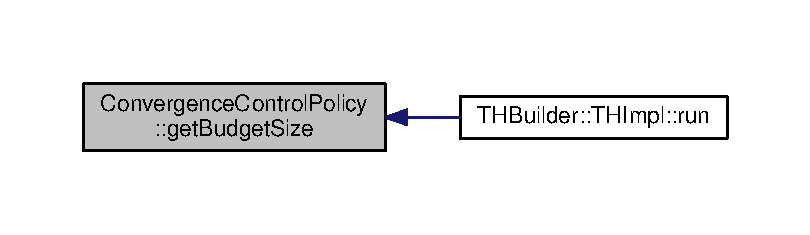
\includegraphics[width=350pt]{classConvergenceControlPolicy_a445c537935922b1bcb67d3732abbfe0f_icgraph}
\end{center}
\end{figure}


\index{Convergence\+Control\+Policy@{Convergence\+Control\+Policy}!run@{run}}
\index{run@{run}!Convergence\+Control\+Policy@{Convergence\+Control\+Policy}}
\subsubsection[{\texorpdfstring{run(\+Search$<$ P, p\+Size, F, f\+Size, V, v\+Size $>$ $\ast$search)=0}{run(Search< P, pSize, F, fSize, V, vSize > *search)=0}}]{\setlength{\rightskip}{0pt plus 5cm}template$<$class P = double, int p\+Size = 1, class F = double, int f\+Size = 1, class V = double, int v\+Size = 1$>$ virtual void {\bf Convergence\+Control\+Policy}$<$ P, p\+Size, F, f\+Size, V, v\+Size $>$\+::run (
\begin{DoxyParamCaption}
\item[{{\bf Search}$<$ P, p\+Size, F, f\+Size, V, v\+Size $>$ $\ast$}]{search}
\end{DoxyParamCaption}
)\hspace{0.3cm}{\ttfamily [pure virtual]}}\hypertarget{classConvergenceControlPolicy_ad72beb5807e87c3fa0602bd0bf4679ac}{}\label{classConvergenceControlPolicy_ad72beb5807e87c3fa0602bd0bf4679ac}


Virtual method that will run, monitor and control one \hyperlink{classTH}{TH} iteration. 

A method implementing this virtual method is the responsible for calling sequential iterations of the actual optimization method, through the call of \hyperlink{classSearch_ae2ea32c6a6ab958e714f19dc71fae9db}{Search\+::next(int)}.


\begin{DoxyParams}{Parameters}
{\em search} & The optimization method. \\
\hline
\end{DoxyParams}


Implemented in \hyperlink{classCSMOn_a430398bc3e096631f8cd180ee1877616}{C\+S\+M\+On$<$ P, p\+Size, F, f\+Size, V, v\+Size $>$}.



Here is the caller graph for this function\+:
\nopagebreak
\begin{figure}[H]
\begin{center}
\leavevmode
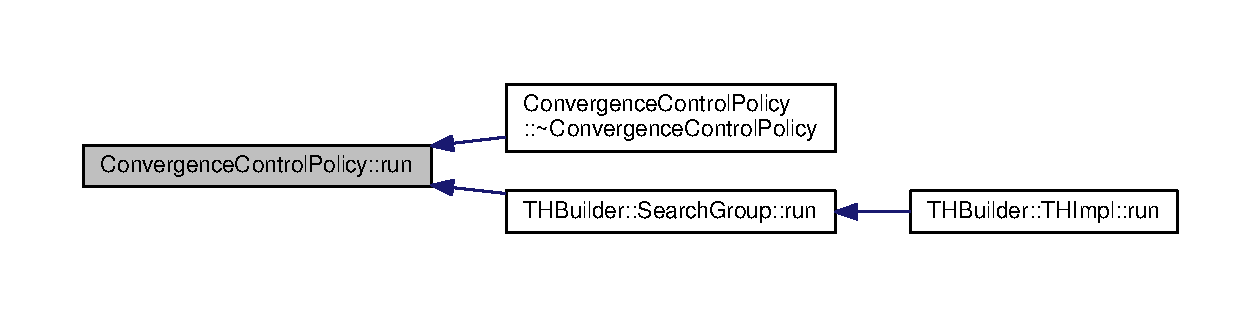
\includegraphics[width=350pt]{classConvergenceControlPolicy_ad72beb5807e87c3fa0602bd0bf4679ac_icgraph}
\end{center}
\end{figure}




The documentation for this class was generated from the following file\+:\begin{DoxyCompactItemize}
\item 
src/\+T\+H/\hyperlink{ConvergenceControlPolicy_8h}{Convergence\+Control\+Policy.\+h}\end{DoxyCompactItemize}

\hypertarget{classConvergentBestListUpdatePolicy}{}\section{Convergent\+Best\+List\+Update\+Policy$<$ P, p\+Size, F, f\+Size, V, v\+Size $>$ Class Template Reference}
\label{classConvergentBestListUpdatePolicy}\index{Convergent\+Best\+List\+Update\+Policy$<$ P, p\+Size, F, f\+Size, V, v\+Size $>$@{Convergent\+Best\+List\+Update\+Policy$<$ P, p\+Size, F, f\+Size, V, v\+Size $>$}}


This policy updates the \hyperlink{classBestList}{Best\+List} instance by enforcing a behavior that speeds up the convergence, as an attempt to reduce the time required to converge and, consequently, increase communication between \hyperlink{classTH}{TH} instances.  




{\ttfamily \#include $<$Convergent\+Best\+List\+Update\+Policy.\+h$>$}



Inheritance diagram for Convergent\+Best\+List\+Update\+Policy$<$ P, p\+Size, F, f\+Size, V, v\+Size $>$\+:
\nopagebreak
\begin{figure}[H]
\begin{center}
\leavevmode
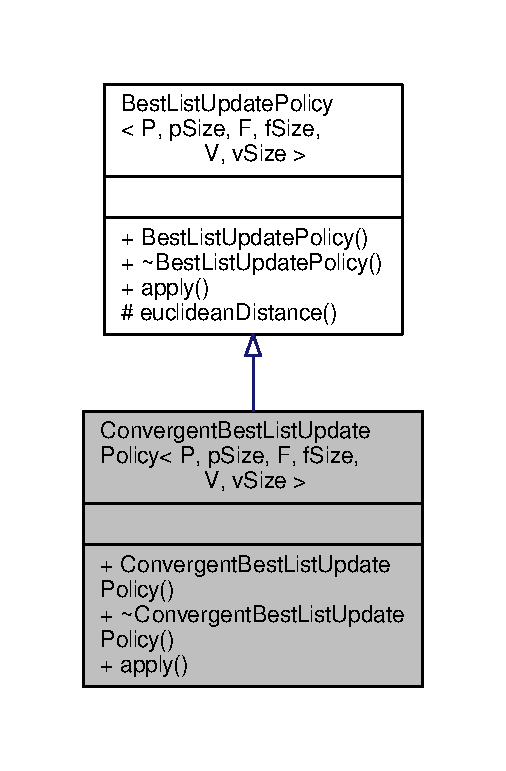
\includegraphics[width=243pt]{classConvergentBestListUpdatePolicy__inherit__graph}
\end{center}
\end{figure}


Collaboration diagram for Convergent\+Best\+List\+Update\+Policy$<$ P, p\+Size, F, f\+Size, V, v\+Size $>$\+:
\nopagebreak
\begin{figure}[H]
\begin{center}
\leavevmode
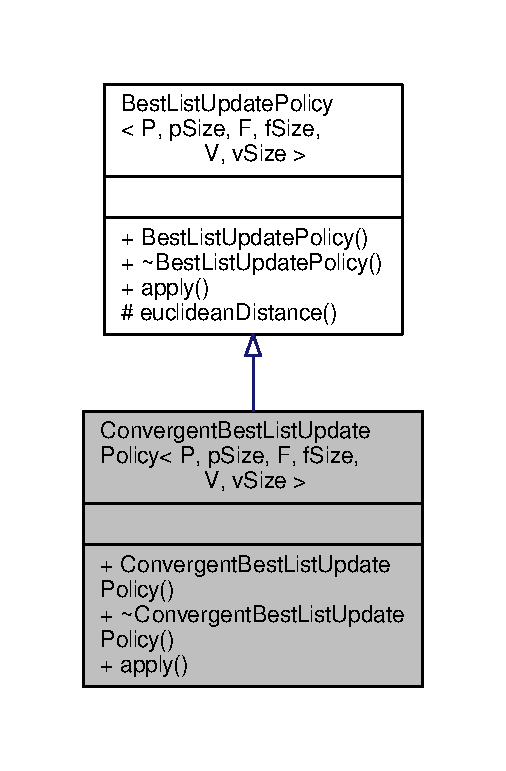
\includegraphics[width=243pt]{classConvergentBestListUpdatePolicy__coll__graph}
\end{center}
\end{figure}
\subsection*{Public Member Functions}
\begin{DoxyCompactItemize}
\item 
\hyperlink{classConvergentBestListUpdatePolicy_a3b4128e26d776ab760e1805beab61747}{Convergent\+Best\+List\+Update\+Policy} ()
\item 
\hyperlink{classConvergentBestListUpdatePolicy_ab965cc3715892b3a1be2559476b91791}{$\sim$\+Convergent\+Best\+List\+Update\+Policy} ()
\item 
void \hyperlink{classConvergentBestListUpdatePolicy_a6382937d32ac8bab7169f216fcd3048f}{apply} (\hyperlink{classBestList}{Best\+List}$<$ P, p\+Size, F, f\+Size, V, v\+Size $>$ $\ast$best\+List, \hyperlink{classSolution}{Solution}$<$ P, p\+Size, F, f\+Size, V, v\+Size $>$ $\ast$solution, \hyperlink{classFitnessPolicy}{Fitness\+Policy}$<$ P, p\+Size, F, f\+Size, V, v\+Size $>$ $\ast$fitness\+Policy)
\begin{DoxyCompactList}\small\item\em This method implements a behavior that focus on convergence speed when updating the solutions from the \hyperlink{classBestList}{Best\+List} instance. \end{DoxyCompactList}\end{DoxyCompactItemize}
\subsection*{Additional Inherited Members}


\subsection{Detailed Description}
\subsubsection*{template$<$class P = double, int p\+Size = 1, class F = double, int f\+Size = 1, class V = double, int v\+Size = 1$>$\\*
class Convergent\+Best\+List\+Update\+Policy$<$ P, p\+Size, F, f\+Size, V, v\+Size $>$}

This policy updates the \hyperlink{classBestList}{Best\+List} instance by enforcing a behavior that speeds up the convergence, as an attempt to reduce the time required to converge and, consequently, increase communication between \hyperlink{classTH}{TH} instances. 

\begin{DoxyAuthor}{Author}
Peter Frank Perroni 
\end{DoxyAuthor}


Definition at line 35 of file Convergent\+Best\+List\+Update\+Policy.\+h.



\subsection{Constructor \& Destructor Documentation}
\index{Convergent\+Best\+List\+Update\+Policy@{Convergent\+Best\+List\+Update\+Policy}!Convergent\+Best\+List\+Update\+Policy@{Convergent\+Best\+List\+Update\+Policy}}
\index{Convergent\+Best\+List\+Update\+Policy@{Convergent\+Best\+List\+Update\+Policy}!Convergent\+Best\+List\+Update\+Policy@{Convergent\+Best\+List\+Update\+Policy}}
\subsubsection[{\texorpdfstring{Convergent\+Best\+List\+Update\+Policy()}{ConvergentBestListUpdatePolicy()}}]{\setlength{\rightskip}{0pt plus 5cm}template$<$class P = double, int p\+Size = 1, class F = double, int f\+Size = 1, class V = double, int v\+Size = 1$>$ {\bf Convergent\+Best\+List\+Update\+Policy}$<$ P, p\+Size, F, f\+Size, V, v\+Size $>$\+::{\bf Convergent\+Best\+List\+Update\+Policy} (
\begin{DoxyParamCaption}
{}
\end{DoxyParamCaption}
)\hspace{0.3cm}{\ttfamily [inline]}}\hypertarget{classConvergentBestListUpdatePolicy_a3b4128e26d776ab760e1805beab61747}{}\label{classConvergentBestListUpdatePolicy_a3b4128e26d776ab760e1805beab61747}


Definition at line 37 of file Convergent\+Best\+List\+Update\+Policy.\+h.

\index{Convergent\+Best\+List\+Update\+Policy@{Convergent\+Best\+List\+Update\+Policy}!````~Convergent\+Best\+List\+Update\+Policy@{$\sim$\+Convergent\+Best\+List\+Update\+Policy}}
\index{````~Convergent\+Best\+List\+Update\+Policy@{$\sim$\+Convergent\+Best\+List\+Update\+Policy}!Convergent\+Best\+List\+Update\+Policy@{Convergent\+Best\+List\+Update\+Policy}}
\subsubsection[{\texorpdfstring{$\sim$\+Convergent\+Best\+List\+Update\+Policy()}{~ConvergentBestListUpdatePolicy()}}]{\setlength{\rightskip}{0pt plus 5cm}template$<$class P = double, int p\+Size = 1, class F = double, int f\+Size = 1, class V = double, int v\+Size = 1$>$ {\bf Convergent\+Best\+List\+Update\+Policy}$<$ P, p\+Size, F, f\+Size, V, v\+Size $>$\+::$\sim${\bf Convergent\+Best\+List\+Update\+Policy} (
\begin{DoxyParamCaption}
{}
\end{DoxyParamCaption}
)\hspace{0.3cm}{\ttfamily [inline]}}\hypertarget{classConvergentBestListUpdatePolicy_ab965cc3715892b3a1be2559476b91791}{}\label{classConvergentBestListUpdatePolicy_ab965cc3715892b3a1be2559476b91791}


Definition at line 38 of file Convergent\+Best\+List\+Update\+Policy.\+h.



\subsection{Member Function Documentation}
\index{Convergent\+Best\+List\+Update\+Policy@{Convergent\+Best\+List\+Update\+Policy}!apply@{apply}}
\index{apply@{apply}!Convergent\+Best\+List\+Update\+Policy@{Convergent\+Best\+List\+Update\+Policy}}
\subsubsection[{\texorpdfstring{apply(\+Best\+List$<$ P, p\+Size, F, f\+Size, V, v\+Size $>$ $\ast$best\+List, Solution$<$ P, p\+Size, F, f\+Size, V, v\+Size $>$ $\ast$solution, Fitness\+Policy$<$ P, p\+Size, F, f\+Size, V, v\+Size $>$ $\ast$fitness\+Policy)}{apply(BestList< P, pSize, F, fSize, V, vSize > *bestList, Solution< P, pSize, F, fSize, V, vSize > *solution, FitnessPolicy< P, pSize, F, fSize, V, vSize > *fitnessPolicy)}}]{\setlength{\rightskip}{0pt plus 5cm}template$<$class P = double, int p\+Size = 1, class F = double, int f\+Size = 1, class V = double, int v\+Size = 1$>$ void {\bf Convergent\+Best\+List\+Update\+Policy}$<$ P, p\+Size, F, f\+Size, V, v\+Size $>$\+::apply (
\begin{DoxyParamCaption}
\item[{{\bf Best\+List}$<$ P, p\+Size, F, f\+Size, V, v\+Size $>$ $\ast$}]{best\+List, }
\item[{{\bf Solution}$<$ P, p\+Size, F, f\+Size, V, v\+Size $>$ $\ast$}]{solution, }
\item[{{\bf Fitness\+Policy}$<$ P, p\+Size, F, f\+Size, V, v\+Size $>$ $\ast$}]{fitness\+Policy}
\end{DoxyParamCaption}
)\hspace{0.3cm}{\ttfamily [inline]}, {\ttfamily [virtual]}}\hypertarget{classConvergentBestListUpdatePolicy_a6382937d32ac8bab7169f216fcd3048f}{}\label{classConvergentBestListUpdatePolicy_a6382937d32ac8bab7169f216fcd3048f}


This method implements a behavior that focus on convergence speed when updating the solutions from the \hyperlink{classBestList}{Best\+List} instance. 


\begin{DoxyParams}{Parameters}
{\em best\+List} & The \hyperlink{classBestList}{Best\+List} instance to be updated. \\
\hline
{\em solution} & The new solution to be added to the best-\/list. \\
\hline
{\em fitness\+Policy} & The \hyperlink{classFitnessPolicy}{Fitness\+Policy} instance capable of evaluating the solutions. \\
\hline
\end{DoxyParams}


Implements \hyperlink{classBestListUpdatePolicy_a591442e3329323b350971b6a55195916}{Best\+List\+Update\+Policy$<$ P, p\+Size, F, f\+Size, V, v\+Size $>$}.



Definition at line 48 of file Convergent\+Best\+List\+Update\+Policy.\+h.



Here is the call graph for this function\+:
\nopagebreak
\begin{figure}[H]
\begin{center}
\leavevmode
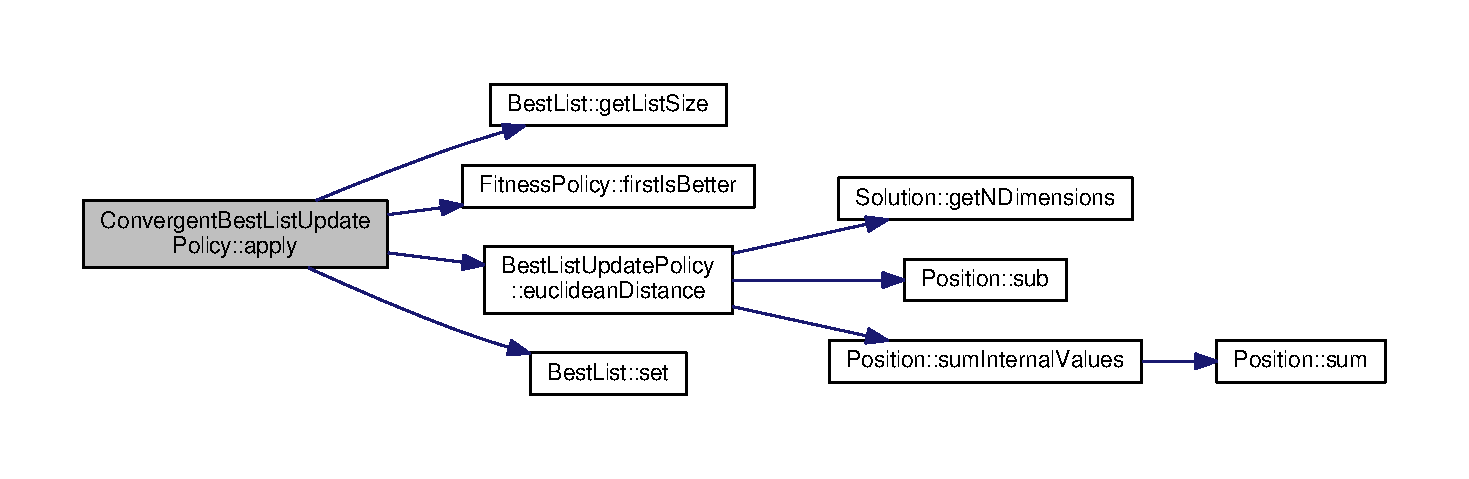
\includegraphics[width=350pt]{classConvergentBestListUpdatePolicy_a6382937d32ac8bab7169f216fcd3048f_cgraph}
\end{center}
\end{figure}




The documentation for this class was generated from the following file\+:\begin{DoxyCompactItemize}
\item 
src/\+T\+H/\hyperlink{ConvergentBestListUpdatePolicy_8h}{Convergent\+Best\+List\+Update\+Policy.\+h}\end{DoxyCompactItemize}

\hypertarget{classCSMOn}{}\section{C\+S\+M\+On$<$ P, p\+Size, F, f\+Size, V, v\+Size $>$ Class Template Reference}
\label{classCSMOn}\index{C\+S\+M\+On$<$ P, p\+Size, F, f\+Size, V, v\+Size $>$@{C\+S\+M\+On$<$ P, p\+Size, F, f\+Size, V, v\+Size $>$}}


This policy runs, monitors and controls the convergence limits for the current \hyperlink{classTH}{TH} iteration.  




{\ttfamily \#include $<$C\+S\+M\+On.\+h$>$}



Inheritance diagram for C\+S\+M\+On$<$ P, p\+Size, F, f\+Size, V, v\+Size $>$\+:\nopagebreak
\begin{figure}[H]
\begin{center}
\leavevmode
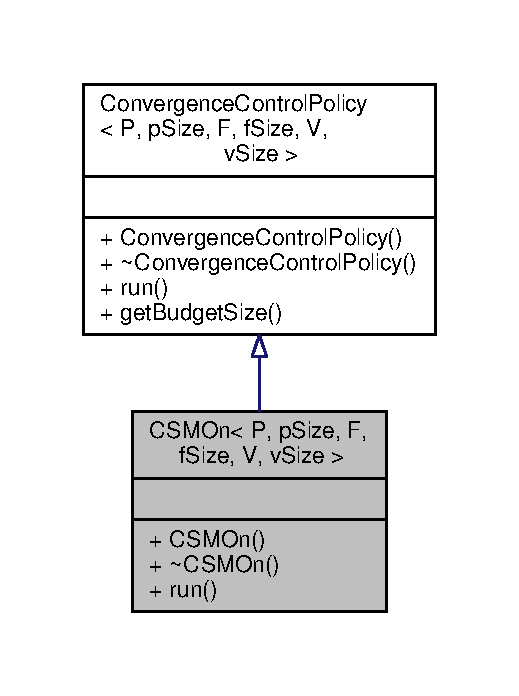
\includegraphics[width=249pt]{classCSMOn__inherit__graph}
\end{center}
\end{figure}


Collaboration diagram for C\+S\+M\+On$<$ P, p\+Size, F, f\+Size, V, v\+Size $>$\+:\nopagebreak
\begin{figure}[H]
\begin{center}
\leavevmode
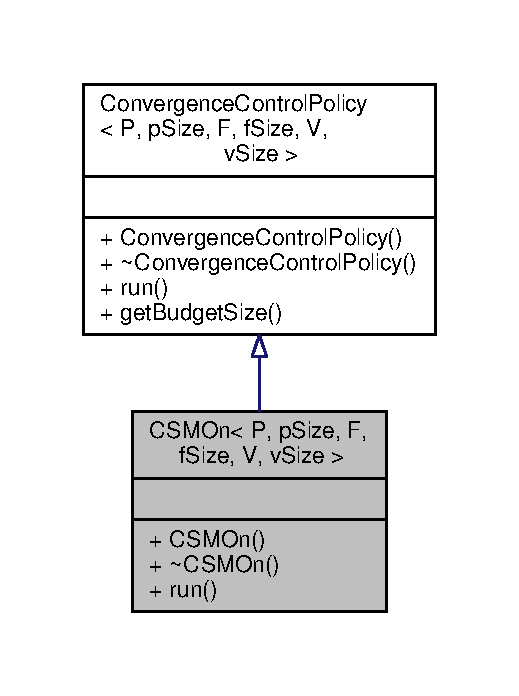
\includegraphics[width=249pt]{classCSMOn__coll__graph}
\end{center}
\end{figure}
\subsection*{Public Member Functions}
\begin{DoxyCompactItemize}
\item 
\hyperlink{classCSMOn_aacd95cee8b48fc2d51120fbf7d2fd546}{C\+S\+M\+On} (int M, double R, F min\+Estimated\+Fit)
\begin{DoxyCompactList}\small\item\em This constructor creates an instance of \hyperlink{classCSMOn}{C\+S\+M\+On}. \end{DoxyCompactList}\item 
\hyperlink{classCSMOn_af77e878e14c14200a4e95457e611162b}{$\sim$\+C\+S\+M\+On} ()
\item 
void \hyperlink{classCSMOn_a430398bc3e096631f8cd180ee1877616}{run} (\hyperlink{classSearch}{Search}$<$ P, p\+Size, F, f\+Size, V, v\+Size $>$ $\ast$search)
\begin{DoxyCompactList}\small\item\em This method runs, monitors and limits the convergence of the optimization method during the current \hyperlink{classTH}{TH} iteration. \end{DoxyCompactList}\end{DoxyCompactItemize}


\subsection{Detailed Description}
\subsubsection*{template$<$class P = double, int p\+Size = 1, class F = double, int f\+Size = 1, class V = double, int v\+Size = 1$>$\\*
class C\+S\+M\+On$<$ P, p\+Size, F, f\+Size, V, v\+Size $>$}

This policy runs, monitors and controls the convergence limits for the current \hyperlink{classTH}{TH} iteration. 

\begin{DoxyAuthor}{Author}
Peter Frank Perroni 
\end{DoxyAuthor}
\begin{DoxyNote}{Note}
For the \hyperlink{classCSMOn}{C\+S\+M\+On} (formerly C\textquotesingle{}M\+On) method, please refer (and cite) to the following paper\+:~\newline
 {\itshape P\+E\+R\+R\+O\+NI, Peter Frank; W\+E\+I\+N\+G\+A\+E\+R\+T\+N\+ER, Daniel; D\+E\+L\+G\+A\+DO, Myriam Regattieri. Estimating stop conditions of swarm based stochastic metaheuristic algorithms. In\+: Proceedings of the Genetic and Evolutionary Computation Conference. 2017. p. 43-\/50.} 
\end{DoxyNote}


Definition at line 50 of file C\+S\+M\+On.\+h.



\subsection{Constructor \& Destructor Documentation}
\index{C\+S\+M\+On@{C\+S\+M\+On}!C\+S\+M\+On@{C\+S\+M\+On}}
\index{C\+S\+M\+On@{C\+S\+M\+On}!C\+S\+M\+On@{C\+S\+M\+On}}
\subsubsection[{\texorpdfstring{C\+S\+M\+On(int M, double R, F min\+Estimated\+Fit)}{CSMOn(int M, double R, F minEstimatedFit)}}]{\setlength{\rightskip}{0pt plus 5cm}template$<$class P = double, int p\+Size = 1, class F = double, int f\+Size = 1, class V = double, int v\+Size = 1$>$ {\bf C\+S\+M\+On}$<$ P, p\+Size, F, f\+Size, V, v\+Size $>$\+::{\bf C\+S\+M\+On} (
\begin{DoxyParamCaption}
\item[{int}]{M, }
\item[{double}]{R, }
\item[{F}]{min\+Estimated\+Fit}
\end{DoxyParamCaption}
)\hspace{0.3cm}{\ttfamily [inline]}}\hypertarget{classCSMOn_aacd95cee8b48fc2d51120fbf7d2fd546}{}\label{classCSMOn_aacd95cee8b48fc2d51120fbf7d2fd546}


This constructor creates an instance of \hyperlink{classCSMOn}{C\+S\+M\+On}. 


\begin{DoxyParams}{Parameters}
{\em M} & The maximum number of fitness function evaluations allowed. \\
\hline
{\em R} & The relaxation factor between \mbox{]}0, 1\mbox{[} that will regulate the acceptance of the convergence stabilization. Larger factors will stop the optimization sooner. \\
\hline
{\em min\+Estimated\+Fit} & The minimum estimated fitness for the problem being optimized (fitness function dependent). \\
\hline
\end{DoxyParams}


Definition at line 157 of file C\+S\+M\+On.\+h.

\index{C\+S\+M\+On@{C\+S\+M\+On}!````~C\+S\+M\+On@{$\sim$\+C\+S\+M\+On}}
\index{````~C\+S\+M\+On@{$\sim$\+C\+S\+M\+On}!C\+S\+M\+On@{C\+S\+M\+On}}
\subsubsection[{\texorpdfstring{$\sim$\+C\+S\+M\+On()}{~CSMOn()}}]{\setlength{\rightskip}{0pt plus 5cm}template$<$class P = double, int p\+Size = 1, class F = double, int f\+Size = 1, class V = double, int v\+Size = 1$>$ {\bf C\+S\+M\+On}$<$ P, p\+Size, F, f\+Size, V, v\+Size $>$\+::$\sim${\bf C\+S\+M\+On} (
\begin{DoxyParamCaption}
{}
\end{DoxyParamCaption}
)\hspace{0.3cm}{\ttfamily [inline]}}\hypertarget{classCSMOn_af77e878e14c14200a4e95457e611162b}{}\label{classCSMOn_af77e878e14c14200a4e95457e611162b}


Definition at line 164 of file C\+S\+M\+On.\+h.



\subsection{Member Function Documentation}
\index{C\+S\+M\+On@{C\+S\+M\+On}!run@{run}}
\index{run@{run}!C\+S\+M\+On@{C\+S\+M\+On}}
\subsubsection[{\texorpdfstring{run(\+Search$<$ P, p\+Size, F, f\+Size, V, v\+Size $>$ $\ast$search)}{run(Search< P, pSize, F, fSize, V, vSize > *search)}}]{\setlength{\rightskip}{0pt plus 5cm}template$<$class P = double, int p\+Size = 1, class F = double, int f\+Size = 1, class V = double, int v\+Size = 1$>$ void {\bf C\+S\+M\+On}$<$ P, p\+Size, F, f\+Size, V, v\+Size $>$\+::run (
\begin{DoxyParamCaption}
\item[{{\bf Search}$<$ P, p\+Size, F, f\+Size, V, v\+Size $>$ $\ast$}]{search}
\end{DoxyParamCaption}
)\hspace{0.3cm}{\ttfamily [inline]}, {\ttfamily [virtual]}}\hypertarget{classCSMOn_a430398bc3e096631f8cd180ee1877616}{}\label{classCSMOn_a430398bc3e096631f8cd180ee1877616}


This method runs, monitors and limits the convergence of the optimization method during the current \hyperlink{classTH}{TH} iteration. 


\begin{DoxyParams}{Parameters}
{\em search} & The optimization method to run. \\
\hline
\end{DoxyParams}


Implements \hyperlink{classConvergenceControlPolicy_ad72beb5807e87c3fa0602bd0bf4679ac}{Convergence\+Control\+Policy$<$ P, p\+Size, F, f\+Size, V, v\+Size $>$}.



Definition at line 174 of file C\+S\+M\+On.\+h.



Here is the call graph for this function\+:\nopagebreak
\begin{figure}[H]
\begin{center}
\leavevmode
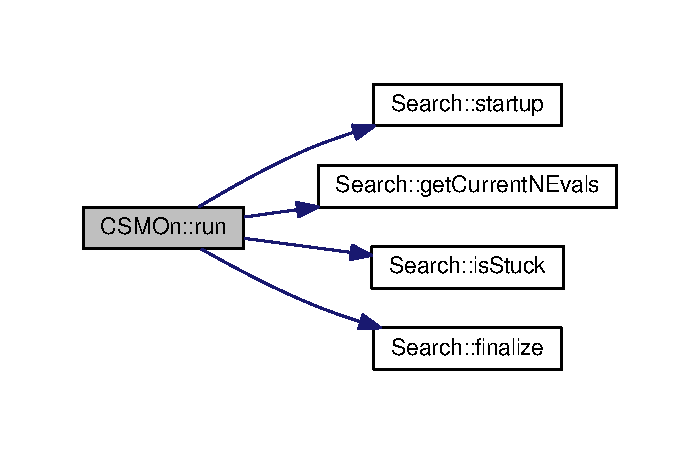
\includegraphics[width=336pt]{classCSMOn_a430398bc3e096631f8cd180ee1877616_cgraph}
\end{center}
\end{figure}




The documentation for this class was generated from the following file\+:\begin{DoxyCompactItemize}
\item 
src/\+T\+H/\hyperlink{CSMOn_8h}{C\+S\+M\+On.\+h}\end{DoxyCompactItemize}

\hypertarget{classDimension}{}\section{Dimension$<$ P $>$ Class Template Reference}
\label{classDimension}\index{Dimension$<$ P $>$@{Dimension$<$ P $>$}}


This class represents the boundaries of a dimension within the search space.  




{\ttfamily \#include $<$Dimension.\+h$>$}



Inheritance diagram for Dimension$<$ P $>$\+:
\nopagebreak
\begin{figure}[H]
\begin{center}
\leavevmode
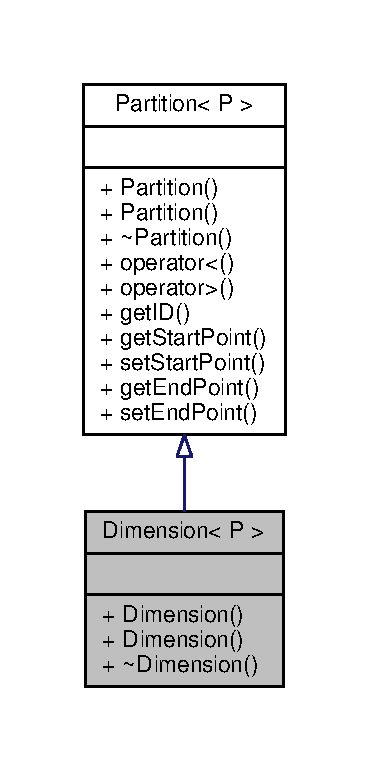
\includegraphics[width=177pt]{classDimension__inherit__graph}
\end{center}
\end{figure}


Collaboration diagram for Dimension$<$ P $>$\+:
\nopagebreak
\begin{figure}[H]
\begin{center}
\leavevmode
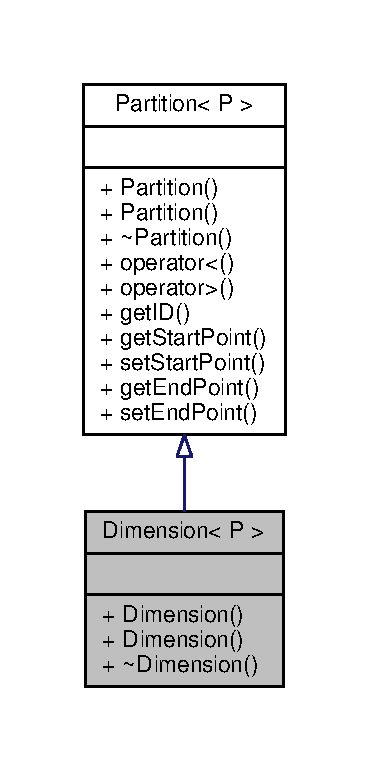
\includegraphics[width=177pt]{classDimension__coll__graph}
\end{center}
\end{figure}
\subsection*{Public Member Functions}
\begin{DoxyCompactItemize}
\item 
\hyperlink{classDimension_a14b3745b4d7691b33a244306c94c6048}{Dimension} (int ID, P start\+Point, P end\+Point)
\item 
\hyperlink{classDimension_a593dbdfb02f5f33fad25d51a083c3a17}{Dimension} (\hyperlink{classPartition}{Partition}$<$ P $>$ $\ast$partition)
\item 
\hyperlink{classDimension_a371288fa5249dcc26e624a60cd28c92f}{$\sim$\+Dimension} ()
\end{DoxyCompactItemize}


\subsection{Detailed Description}
\subsubsection*{template$<$class P = double$>$\\*
class Dimension$<$ P $>$}

This class represents the boundaries of a dimension within the search space. 

\begin{DoxyAuthor}{Author}
Peter Frank Perroni 
\end{DoxyAuthor}


Definition at line 33 of file Dimension.\+h.



\subsection{Constructor \& Destructor Documentation}
\index{Dimension@{Dimension}!Dimension@{Dimension}}
\index{Dimension@{Dimension}!Dimension@{Dimension}}
\subsubsection[{\texorpdfstring{Dimension(int I\+D, P start\+Point, P end\+Point)}{Dimension(int ID, P startPoint, P endPoint)}}]{\setlength{\rightskip}{0pt plus 5cm}template$<$class P = double$>$ {\bf Dimension}$<$ P $>$\+::{\bf Dimension} (
\begin{DoxyParamCaption}
\item[{int}]{ID, }
\item[{P}]{start\+Point, }
\item[{P}]{end\+Point}
\end{DoxyParamCaption}
)\hspace{0.3cm}{\ttfamily [inline]}}\hypertarget{classDimension_a14b3745b4d7691b33a244306c94c6048}{}\label{classDimension_a14b3745b4d7691b33a244306c94c6048}


Definition at line 35 of file Dimension.\+h.

\index{Dimension@{Dimension}!Dimension@{Dimension}}
\index{Dimension@{Dimension}!Dimension@{Dimension}}
\subsubsection[{\texorpdfstring{Dimension(\+Partition$<$ P $>$ $\ast$partition)}{Dimension(Partition< P > *partition)}}]{\setlength{\rightskip}{0pt plus 5cm}template$<$class P = double$>$ {\bf Dimension}$<$ P $>$\+::{\bf Dimension} (
\begin{DoxyParamCaption}
\item[{{\bf Partition}$<$ P $>$ $\ast$}]{partition}
\end{DoxyParamCaption}
)\hspace{0.3cm}{\ttfamily [inline]}}\hypertarget{classDimension_a593dbdfb02f5f33fad25d51a083c3a17}{}\label{classDimension_a593dbdfb02f5f33fad25d51a083c3a17}


Definition at line 36 of file Dimension.\+h.

\index{Dimension@{Dimension}!````~Dimension@{$\sim$\+Dimension}}
\index{````~Dimension@{$\sim$\+Dimension}!Dimension@{Dimension}}
\subsubsection[{\texorpdfstring{$\sim$\+Dimension()}{~Dimension()}}]{\setlength{\rightskip}{0pt plus 5cm}template$<$class P = double$>$ {\bf Dimension}$<$ P $>$\+::$\sim${\bf Dimension} (
\begin{DoxyParamCaption}
{}
\end{DoxyParamCaption}
)\hspace{0.3cm}{\ttfamily [inline]}}\hypertarget{classDimension_a371288fa5249dcc26e624a60cd28c92f}{}\label{classDimension_a371288fa5249dcc26e624a60cd28c92f}


Definition at line 37 of file Dimension.\+h.



The documentation for this class was generated from the following file\+:\begin{DoxyCompactItemize}
\item 
src/\+T\+H/\hyperlink{Dimension_8h}{Dimension.\+h}\end{DoxyCompactItemize}

\hypertarget{classDivergentBestListUpdatePolicy}{}\section{Divergent\+Best\+List\+Update\+Policy$<$ P, p\+Size, F, f\+Size, V, v\+Size $>$ Class Template Reference}
\label{classDivergentBestListUpdatePolicy}\index{Divergent\+Best\+List\+Update\+Policy$<$ P, p\+Size, F, f\+Size, V, v\+Size $>$@{Divergent\+Best\+List\+Update\+Policy$<$ P, p\+Size, F, f\+Size, V, v\+Size $>$}}


This policy updates the \hyperlink{classBestList}{Best\+List} instance by enforcing a behavior that slows down the convergence, as an attempt to increase the exploration and, consequently, the diversity of solutions.  




{\ttfamily \#include $<$Divergent\+Best\+List\+Update\+Policy.\+h$>$}



Inheritance diagram for Divergent\+Best\+List\+Update\+Policy$<$ P, p\+Size, F, f\+Size, V, v\+Size $>$\+:
\nopagebreak
\begin{figure}[H]
\begin{center}
\leavevmode
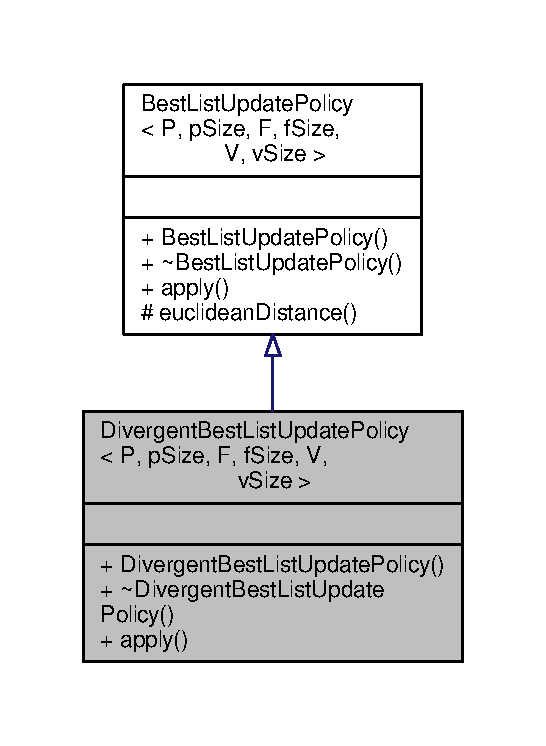
\includegraphics[width=262pt]{classDivergentBestListUpdatePolicy__inherit__graph}
\end{center}
\end{figure}


Collaboration diagram for Divergent\+Best\+List\+Update\+Policy$<$ P, p\+Size, F, f\+Size, V, v\+Size $>$\+:
\nopagebreak
\begin{figure}[H]
\begin{center}
\leavevmode
\includegraphics[width=262pt]{classDivergentBestListUpdatePolicy__coll__graph}
\end{center}
\end{figure}
\subsection*{Public Member Functions}
\begin{DoxyCompactItemize}
\item 
\hyperlink{classDivergentBestListUpdatePolicy_a9f071374e5db075f1ce1e6cba1bfa1a1}{Divergent\+Best\+List\+Update\+Policy} ()
\item 
\hyperlink{classDivergentBestListUpdatePolicy_a8c0f47b6ca1693a298c170f73d1f2d21}{$\sim$\+Divergent\+Best\+List\+Update\+Policy} ()
\item 
void \hyperlink{classDivergentBestListUpdatePolicy_a793d47a0c458eef94b27fbee73e5df0e}{apply} (\hyperlink{classBestList}{Best\+List}$<$ P, p\+Size, F, f\+Size, V, v\+Size $>$ $\ast$best\+List, \hyperlink{classSolution}{Solution}$<$ P, p\+Size, F, f\+Size, V, v\+Size $>$ $\ast$solution, \hyperlink{classFitnessPolicy}{Fitness\+Policy}$<$ P, p\+Size, F, f\+Size, V, v\+Size $>$ $\ast$fitness\+Policy)
\begin{DoxyCompactList}\small\item\em This method implements a behavior that promotes diversity when updating the solutions from the \hyperlink{classBestList}{Best\+List} instance. \end{DoxyCompactList}\end{DoxyCompactItemize}
\subsection*{Additional Inherited Members}


\subsection{Detailed Description}
\subsubsection*{template$<$class P = double, int p\+Size = 1, class F = double, int f\+Size = 1, class V = double, int v\+Size = 1$>$\\*
class Divergent\+Best\+List\+Update\+Policy$<$ P, p\+Size, F, f\+Size, V, v\+Size $>$}

This policy updates the \hyperlink{classBestList}{Best\+List} instance by enforcing a behavior that slows down the convergence, as an attempt to increase the exploration and, consequently, the diversity of solutions. 

\begin{DoxyAuthor}{Author}
Peter Frank Perroni 
\end{DoxyAuthor}


Definition at line 35 of file Divergent\+Best\+List\+Update\+Policy.\+h.



\subsection{Constructor \& Destructor Documentation}
\index{Divergent\+Best\+List\+Update\+Policy@{Divergent\+Best\+List\+Update\+Policy}!Divergent\+Best\+List\+Update\+Policy@{Divergent\+Best\+List\+Update\+Policy}}
\index{Divergent\+Best\+List\+Update\+Policy@{Divergent\+Best\+List\+Update\+Policy}!Divergent\+Best\+List\+Update\+Policy@{Divergent\+Best\+List\+Update\+Policy}}
\subsubsection[{\texorpdfstring{Divergent\+Best\+List\+Update\+Policy()}{DivergentBestListUpdatePolicy()}}]{\setlength{\rightskip}{0pt plus 5cm}template$<$class P  = double, int p\+Size = 1, class F  = double, int f\+Size = 1, class V  = double, int v\+Size = 1$>$ {\bf Divergent\+Best\+List\+Update\+Policy}$<$ P, p\+Size, F, f\+Size, V, v\+Size $>$\+::{\bf Divergent\+Best\+List\+Update\+Policy} (
\begin{DoxyParamCaption}
{}
\end{DoxyParamCaption}
)\hspace{0.3cm}{\ttfamily [inline]}}\hypertarget{classDivergentBestListUpdatePolicy_a9f071374e5db075f1ce1e6cba1bfa1a1}{}\label{classDivergentBestListUpdatePolicy_a9f071374e5db075f1ce1e6cba1bfa1a1}


Definition at line 37 of file Divergent\+Best\+List\+Update\+Policy.\+h.

\index{Divergent\+Best\+List\+Update\+Policy@{Divergent\+Best\+List\+Update\+Policy}!````~Divergent\+Best\+List\+Update\+Policy@{$\sim$\+Divergent\+Best\+List\+Update\+Policy}}
\index{````~Divergent\+Best\+List\+Update\+Policy@{$\sim$\+Divergent\+Best\+List\+Update\+Policy}!Divergent\+Best\+List\+Update\+Policy@{Divergent\+Best\+List\+Update\+Policy}}
\subsubsection[{\texorpdfstring{$\sim$\+Divergent\+Best\+List\+Update\+Policy()}{~DivergentBestListUpdatePolicy()}}]{\setlength{\rightskip}{0pt plus 5cm}template$<$class P  = double, int p\+Size = 1, class F  = double, int f\+Size = 1, class V  = double, int v\+Size = 1$>$ {\bf Divergent\+Best\+List\+Update\+Policy}$<$ P, p\+Size, F, f\+Size, V, v\+Size $>$\+::$\sim${\bf Divergent\+Best\+List\+Update\+Policy} (
\begin{DoxyParamCaption}
{}
\end{DoxyParamCaption}
)\hspace{0.3cm}{\ttfamily [inline]}}\hypertarget{classDivergentBestListUpdatePolicy_a8c0f47b6ca1693a298c170f73d1f2d21}{}\label{classDivergentBestListUpdatePolicy_a8c0f47b6ca1693a298c170f73d1f2d21}


Definition at line 38 of file Divergent\+Best\+List\+Update\+Policy.\+h.



\subsection{Member Function Documentation}
\index{Divergent\+Best\+List\+Update\+Policy@{Divergent\+Best\+List\+Update\+Policy}!apply@{apply}}
\index{apply@{apply}!Divergent\+Best\+List\+Update\+Policy@{Divergent\+Best\+List\+Update\+Policy}}
\subsubsection[{\texorpdfstring{apply(\+Best\+List$<$ P, p\+Size, F, f\+Size, V, v\+Size $>$ $\ast$best\+List, Solution$<$ P, p\+Size, F, f\+Size, V, v\+Size $>$ $\ast$solution, Fitness\+Policy$<$ P, p\+Size, F, f\+Size, V, v\+Size $>$ $\ast$fitness\+Policy)}{apply(BestList< P, pSize, F, fSize, V, vSize > *bestList, Solution< P, pSize, F, fSize, V, vSize > *solution, FitnessPolicy< P, pSize, F, fSize, V, vSize > *fitnessPolicy)}}]{\setlength{\rightskip}{0pt plus 5cm}template$<$class P  = double, int p\+Size = 1, class F  = double, int f\+Size = 1, class V  = double, int v\+Size = 1$>$ void {\bf Divergent\+Best\+List\+Update\+Policy}$<$ P, p\+Size, F, f\+Size, V, v\+Size $>$\+::apply (
\begin{DoxyParamCaption}
\item[{{\bf Best\+List}$<$ P, p\+Size, F, f\+Size, V, v\+Size $>$ $\ast$}]{best\+List, }
\item[{{\bf Solution}$<$ P, p\+Size, F, f\+Size, V, v\+Size $>$ $\ast$}]{solution, }
\item[{{\bf Fitness\+Policy}$<$ P, p\+Size, F, f\+Size, V, v\+Size $>$ $\ast$}]{fitness\+Policy}
\end{DoxyParamCaption}
)\hspace{0.3cm}{\ttfamily [inline]}, {\ttfamily [virtual]}}\hypertarget{classDivergentBestListUpdatePolicy_a793d47a0c458eef94b27fbee73e5df0e}{}\label{classDivergentBestListUpdatePolicy_a793d47a0c458eef94b27fbee73e5df0e}


This method implements a behavior that promotes diversity when updating the solutions from the \hyperlink{classBestList}{Best\+List} instance. 


\begin{DoxyParams}{Parameters}
{\em best\+List} & The \hyperlink{classBestList}{Best\+List} instance to be updated. \\
\hline
{\em solution} & The new solution to be added to the best-\/list. \\
\hline
{\em fitness\+Policy} & The \hyperlink{classFitnessPolicy}{Fitness\+Policy} instance capable of evaluating the solutions. \\
\hline
\end{DoxyParams}


Implements \hyperlink{classBestListUpdatePolicy_a591442e3329323b350971b6a55195916}{Best\+List\+Update\+Policy$<$ P, p\+Size, F, f\+Size, V, v\+Size $>$}.



Definition at line 48 of file Divergent\+Best\+List\+Update\+Policy.\+h.



Here is the call graph for this function\+:
\nopagebreak
\begin{figure}[H]
\begin{center}
\leavevmode
\includegraphics[width=350pt]{classDivergentBestListUpdatePolicy_a793d47a0c458eef94b27fbee73e5df0e_cgraph}
\end{center}
\end{figure}




The documentation for this class was generated from the following file\+:\begin{DoxyCompactItemize}
\item 
src/\+T\+H/\hyperlink{DivergentBestListUpdatePolicy_8h}{Divergent\+Best\+List\+Update\+Policy.\+h}\end{DoxyCompactItemize}

\hypertarget{structFitness}{}\section{Fitness$<$ F, f\+Size $>$ Class Template Reference}
\label{structFitness}\index{Fitness$<$ F, f\+Size $>$@{Fitness$<$ F, f\+Size $>$}}


This structure represents the fitness (or cost) of one \hyperlink{classSolution}{Solution}.  




{\ttfamily \#include $<$Fitness.\+h$>$}



Collaboration diagram for Fitness$<$ F, f\+Size $>$\+:
\nopagebreak
\begin{figure}[H]
\begin{center}
\leavevmode
\includegraphics[width=203pt]{structFitness__coll__graph}
\end{center}
\end{figure}
\subsection*{Public Member Functions}
\begin{DoxyCompactItemize}
\item 
void \hyperlink{structFitness_a73ef98fc5780e1e15bbfac6177bd5c5a}{check\+Compatibility} (\hyperlink{structFitness}{Fitness}$<$ F, f\+Size $>$ $\ast$fitness)
\item 
void \hyperlink{structFitness_a557b47961eb4a4589c53ee54f975e65e}{operator=} (F $\ast$buffer)
\begin{DoxyCompactList}\small\item\em Operator that assigns the values of a buffer to the list that represents the current \hyperlink{structFitness}{Fitness}. \end{DoxyCompactList}\item 
void \hyperlink{structFitness_a19e4c2cc608e17611deacc194d83dc89}{operator=} (\hyperlink{structFitness}{Fitness}$<$ F, f\+Size $>$ $\ast$fitness)
\begin{DoxyCompactList}\small\item\em Operator that overrides the contents of this fitness with the contents of the \hyperlink{structFitness}{Fitness} instance received. \end{DoxyCompactList}\item 
void \hyperlink{structFitness_afd45c5c802ca9d0086685e85730f13da}{operator=} (\hyperlink{structFitness}{Fitness}$<$ F, f\+Size $>$ \&fitness)
\begin{DoxyCompactList}\small\item\em Operator that overrides the contents of this fitness with the contents of the \hyperlink{structFitness}{Fitness} instance received. \end{DoxyCompactList}\item 
void \hyperlink{structFitness_a875d901a35662cf786bcc17b9e1a6983}{operator=} (F value)
\begin{DoxyCompactList}\small\item\em Operator that assigns the same value to all elements of the list that represents the current \hyperlink{structFitness}{Fitness}. \end{DoxyCompactList}\item 
bool \hyperlink{structFitness_abd044181ac7240fa59c7a25fbcca5150}{equals} (F $\ast$buffer)
\begin{DoxyCompactList}\small\item\em Compares the current fitness with the buffer received. \end{DoxyCompactList}\item 
bool \hyperlink{structFitness_acfc0528bc5ec716f1c06a58086c59b50}{equals} (\hyperlink{structFitness}{Fitness}$<$ F, f\+Size $>$ $\ast$fitness)
\begin{DoxyCompactList}\small\item\em Compares the current fitness with the fitness received. \end{DoxyCompactList}\item 
bool \hyperlink{structFitness_a87880c3a43c0bf6068c687d71e96bbfc}{operator==} (\hyperlink{structFitness}{Fitness}$<$ F, f\+Size $>$ $\ast$fitness)
\item 
bool \hyperlink{structFitness_a525bb798a0016fada60e60a601c46510}{operator==} (\hyperlink{structFitness}{Fitness}$<$ F, f\+Size $>$ \&fitness)
\item 
bool \hyperlink{structFitness_a4cab5f7960366b61b34213efc89a4288}{operator!=} (\hyperlink{structFitness}{Fitness}$<$ F, f\+Size $>$ $\ast$fitness)
\item 
bool \hyperlink{structFitness_a01be3acc37c269b11b2697d135759f20}{operator!=} (\hyperlink{structFitness}{Fitness}$<$ F, f\+Size $>$ \&fitness)
\item 
F \hyperlink{structFitness_a50bf7f366d9e182293184ebee7297df1}{get\+Internal\+Fitness} (int i)
\begin{DoxyCompactList}\small\item\em Get a partial fitness based on its index in the list of values that represents the actual \hyperlink{structFitness}{Fitness}. \end{DoxyCompactList}\item 
F $\ast$ \hyperlink{structFitness_ab25220be9e68b4737a91a7b307c5e4d5}{get\+Internal\+Fitness} ()
\begin{DoxyCompactList}\small\item\em Get a pointer to the actual list of values that represents the \hyperlink{structFitness}{Fitness}. \end{DoxyCompactList}\item 
void \hyperlink{structFitness_aeb0b0935f54a9798faf30ddb4216d10a}{get\+Internal\+Fitness} (F $\ast$buffer)
\begin{DoxyCompactList}\small\item\em This method copies the contents of current \hyperlink{structFitness}{Fitness} to the buffer received. \end{DoxyCompactList}\item 
F \hyperlink{structFitness_ac6513eb1ca76f5618cbc0a2f4e25139c}{get\+First\+Value} ()
\begin{DoxyCompactList}\small\item\em Get the first value from the list of values that represents the \hyperlink{structFitness}{Fitness}. \end{DoxyCompactList}\item 
int \hyperlink{structFitness_acebcc12ee16b4c1a95f9a16c0ba82191}{get\+Fitness\+Size} ()
\begin{DoxyCompactList}\small\item\em Get the number of values that represents a \hyperlink{structFitness}{Fitness}. \end{DoxyCompactList}\end{DoxyCompactItemize}
\subsection*{Data Fields}
\begin{DoxyCompactItemize}
\item 
F \hyperlink{structFitness_abffc9af3988e39e82dc81fc006e6ef4a}{internal\+Fitness} \mbox{[}f\+Size\mbox{]}
\item 
int \hyperlink{structFitness_ab487af790e21882d9308356e9b8fbf0d}{size} = f\+Size
\end{DoxyCompactItemize}


\subsection{Detailed Description}
\subsubsection*{template$<$class F = double, int f\+Size = 1$>$\\*
class Fitness$<$ F, f\+Size $>$}

This structure represents the fitness (or cost) of one \hyperlink{classSolution}{Solution}. 

\begin{DoxyAuthor}{Author}
Peter Frank Perroni
\end{DoxyAuthor}
A \hyperlink{structFitness}{Fitness} on \hyperlink{classTH}{TH} can be represented by multiple values, instead of the traditional 1-\/value fitness (eg. multi-\/objective optimization, fitness history, score list, etc). The fitness is an ordered list with any number of elements, whose type must be of same basic data type for all elements (eg., double or int). 

Definition at line 37 of file Fitness.\+h.



\subsection{Member Function Documentation}
\index{Fitness@{Fitness}!check\+Compatibility@{check\+Compatibility}}
\index{check\+Compatibility@{check\+Compatibility}!Fitness@{Fitness}}
\subsubsection[{\texorpdfstring{check\+Compatibility(\+Fitness$<$ F, f\+Size $>$ $\ast$fitness)}{checkCompatibility(Fitness< F, fSize > *fitness)}}]{\setlength{\rightskip}{0pt plus 5cm}template$<$class F = double, int f\+Size = 1$>$ void {\bf Fitness}$<$ F, f\+Size $>$\+::check\+Compatibility (
\begin{DoxyParamCaption}
\item[{{\bf Fitness}$<$ F, f\+Size $>$ $\ast$}]{fitness}
\end{DoxyParamCaption}
)\hspace{0.3cm}{\ttfamily [inline]}}\hypertarget{structFitness_a73ef98fc5780e1e15bbfac6177bd5c5a}{}\label{structFitness_a73ef98fc5780e1e15bbfac6177bd5c5a}


Definition at line 41 of file Fitness.\+h.



Here is the caller graph for this function\+:
\nopagebreak
\begin{figure}[H]
\begin{center}
\leavevmode
\includegraphics[width=350pt]{structFitness_a73ef98fc5780e1e15bbfac6177bd5c5a_icgraph}
\end{center}
\end{figure}


\index{Fitness@{Fitness}!equals@{equals}}
\index{equals@{equals}!Fitness@{Fitness}}
\subsubsection[{\texorpdfstring{equals(\+F $\ast$buffer)}{equals(F *buffer)}}]{\setlength{\rightskip}{0pt plus 5cm}template$<$class F = double, int f\+Size = 1$>$ bool {\bf Fitness}$<$ F, f\+Size $>$\+::equals (
\begin{DoxyParamCaption}
\item[{F $\ast$}]{buffer}
\end{DoxyParamCaption}
)\hspace{0.3cm}{\ttfamily [inline]}}\hypertarget{structFitness_abd044181ac7240fa59c7a25fbcca5150}{}\label{structFitness_abd044181ac7240fa59c7a25fbcca5150}


Compares the current fitness with the buffer received. 

The buffer size must be compatible with this \hyperlink{structFitness}{Fitness}.


\begin{DoxyParams}{Parameters}
{\em buffer} & The buffer to compare. \\
\hline
\end{DoxyParams}
\begin{DoxyReturn}{Returns}
True if this \hyperlink{structFitness}{Fitness} instance has the same contents as the buffer received. False otherwise. 
\end{DoxyReturn}


Definition at line 108 of file Fitness.\+h.



Here is the caller graph for this function\+:
\nopagebreak
\begin{figure}[H]
\begin{center}
\leavevmode
\includegraphics[width=316pt]{structFitness_abd044181ac7240fa59c7a25fbcca5150_icgraph}
\end{center}
\end{figure}


\index{Fitness@{Fitness}!equals@{equals}}
\index{equals@{equals}!Fitness@{Fitness}}
\subsubsection[{\texorpdfstring{equals(\+Fitness$<$ F, f\+Size $>$ $\ast$fitness)}{equals(Fitness< F, fSize > *fitness)}}]{\setlength{\rightskip}{0pt plus 5cm}template$<$class F = double, int f\+Size = 1$>$ bool {\bf Fitness}$<$ F, f\+Size $>$\+::equals (
\begin{DoxyParamCaption}
\item[{{\bf Fitness}$<$ F, f\+Size $>$ $\ast$}]{fitness}
\end{DoxyParamCaption}
)\hspace{0.3cm}{\ttfamily [inline]}}\hypertarget{structFitness_acfc0528bc5ec716f1c06a58086c59b50}{}\label{structFitness_acfc0528bc5ec716f1c06a58086c59b50}


Compares the current fitness with the fitness received. 


\begin{DoxyParams}{Parameters}
{\em fitness} & The \hyperlink{structFitness}{Fitness} instance to compare. \\
\hline
\end{DoxyParams}
\begin{DoxyReturn}{Returns}
True if this \hyperlink{structFitness}{Fitness} instance has the same contents as the fitness received. False otherwise. 
\end{DoxyReturn}

\begin{DoxyExceptions}{Exceptions}
{\em invalid\+\_\+argument} & if the fitness received is not compatible with current fitness. \\
\hline
\end{DoxyExceptions}


Definition at line 123 of file Fitness.\+h.



Here is the call graph for this function\+:
\nopagebreak
\begin{figure}[H]
\begin{center}
\leavevmode
\includegraphics[width=350pt]{structFitness_acfc0528bc5ec716f1c06a58086c59b50_cgraph}
\end{center}
\end{figure}


\index{Fitness@{Fitness}!get\+First\+Value@{get\+First\+Value}}
\index{get\+First\+Value@{get\+First\+Value}!Fitness@{Fitness}}
\subsubsection[{\texorpdfstring{get\+First\+Value()}{getFirstValue()}}]{\setlength{\rightskip}{0pt plus 5cm}template$<$class F = double, int f\+Size = 1$>$ F {\bf Fitness}$<$ F, f\+Size $>$\+::get\+First\+Value (
\begin{DoxyParamCaption}
{}
\end{DoxyParamCaption}
)\hspace{0.3cm}{\ttfamily [inline]}}\hypertarget{structFitness_ac6513eb1ca76f5618cbc0a2f4e25139c}{}\label{structFitness_ac6513eb1ca76f5618cbc0a2f4e25139c}


Get the first value from the list of values that represents the \hyperlink{structFitness}{Fitness}. 

Useful when the fitness is represented by 1 single value.

\begin{DoxyReturn}{Returns}
The first value from the list of values that represents the fitness (or cost). 
\end{DoxyReturn}


Definition at line 183 of file Fitness.\+h.



Here is the caller graph for this function\+:
\nopagebreak
\begin{figure}[H]
\begin{center}
\leavevmode
\includegraphics[width=350pt]{structFitness_ac6513eb1ca76f5618cbc0a2f4e25139c_icgraph}
\end{center}
\end{figure}


\index{Fitness@{Fitness}!get\+Fitness\+Size@{get\+Fitness\+Size}}
\index{get\+Fitness\+Size@{get\+Fitness\+Size}!Fitness@{Fitness}}
\subsubsection[{\texorpdfstring{get\+Fitness\+Size()}{getFitnessSize()}}]{\setlength{\rightskip}{0pt plus 5cm}template$<$class F = double, int f\+Size = 1$>$ int {\bf Fitness}$<$ F, f\+Size $>$\+::get\+Fitness\+Size (
\begin{DoxyParamCaption}
{}
\end{DoxyParamCaption}
)\hspace{0.3cm}{\ttfamily [inline]}}\hypertarget{structFitness_acebcc12ee16b4c1a95f9a16c0ba82191}{}\label{structFitness_acebcc12ee16b4c1a95f9a16c0ba82191}


Get the number of values that represents a \hyperlink{structFitness}{Fitness}. 

\begin{DoxyReturn}{Returns}
The number of values that represents a \hyperlink{structFitness}{Fitness}. 
\end{DoxyReturn}


Definition at line 189 of file Fitness.\+h.

\index{Fitness@{Fitness}!get\+Internal\+Fitness@{get\+Internal\+Fitness}}
\index{get\+Internal\+Fitness@{get\+Internal\+Fitness}!Fitness@{Fitness}}
\subsubsection[{\texorpdfstring{get\+Internal\+Fitness(int i)}{getInternalFitness(int i)}}]{\setlength{\rightskip}{0pt plus 5cm}template$<$class F = double, int f\+Size = 1$>$ F {\bf Fitness}$<$ F, f\+Size $>$\+::get\+Internal\+Fitness (
\begin{DoxyParamCaption}
\item[{int}]{i}
\end{DoxyParamCaption}
)\hspace{0.3cm}{\ttfamily [inline]}}\hypertarget{structFitness_a50bf7f366d9e182293184ebee7297df1}{}\label{structFitness_a50bf7f366d9e182293184ebee7297df1}


Get a partial fitness based on its index in the list of values that represents the actual \hyperlink{structFitness}{Fitness}. 

Given that a \hyperlink{structFitness}{Fitness} can be represented by multiple values, a \char`\"{}partial fitness\char`\"{} here actually means one of the values that represents a single fitness (or cost).


\begin{DoxyParams}{Parameters}
{\em i} & The index of the partial fitness in the list (index list starts in zero). \\
\hline
\end{DoxyParams}
\begin{DoxyReturn}{Returns}
The partial fitness selected. 
\end{DoxyReturn}


Definition at line 150 of file Fitness.\+h.



Here is the caller graph for this function\+:
\nopagebreak
\begin{figure}[H]
\begin{center}
\leavevmode
\includegraphics[width=350pt]{structFitness_a50bf7f366d9e182293184ebee7297df1_icgraph}
\end{center}
\end{figure}


\index{Fitness@{Fitness}!get\+Internal\+Fitness@{get\+Internal\+Fitness}}
\index{get\+Internal\+Fitness@{get\+Internal\+Fitness}!Fitness@{Fitness}}
\subsubsection[{\texorpdfstring{get\+Internal\+Fitness()}{getInternalFitness()}}]{\setlength{\rightskip}{0pt plus 5cm}template$<$class F = double, int f\+Size = 1$>$ F$\ast$ {\bf Fitness}$<$ F, f\+Size $>$\+::get\+Internal\+Fitness (
\begin{DoxyParamCaption}
{}
\end{DoxyParamCaption}
)\hspace{0.3cm}{\ttfamily [inline]}}\hypertarget{structFitness_ab25220be9e68b4737a91a7b307c5e4d5}{}\label{structFitness_ab25220be9e68b4737a91a7b307c5e4d5}


Get a pointer to the actual list of values that represents the \hyperlink{structFitness}{Fitness}. 

\begin{DoxyReturn}{Returns}
The pointer to the fitness\textquotesingle{}s values. 
\end{DoxyReturn}


Definition at line 159 of file Fitness.\+h.

\index{Fitness@{Fitness}!get\+Internal\+Fitness@{get\+Internal\+Fitness}}
\index{get\+Internal\+Fitness@{get\+Internal\+Fitness}!Fitness@{Fitness}}
\subsubsection[{\texorpdfstring{get\+Internal\+Fitness(\+F $\ast$buffer)}{getInternalFitness(F *buffer)}}]{\setlength{\rightskip}{0pt plus 5cm}template$<$class F = double, int f\+Size = 1$>$ void {\bf Fitness}$<$ F, f\+Size $>$\+::get\+Internal\+Fitness (
\begin{DoxyParamCaption}
\item[{F $\ast$}]{buffer}
\end{DoxyParamCaption}
)\hspace{0.3cm}{\ttfamily [inline]}}\hypertarget{structFitness_aeb0b0935f54a9798faf30ddb4216d10a}{}\label{structFitness_aeb0b0935f54a9798faf30ddb4216d10a}


This method copies the contents of current \hyperlink{structFitness}{Fitness} to the buffer received. 

The buffer size must be compatible with this \hyperlink{structFitness}{Fitness}.


\begin{DoxyParams}{Parameters}
{\em buffer} & The destination buffer. \\
\hline
\end{DoxyParams}


Definition at line 169 of file Fitness.\+h.

\index{Fitness@{Fitness}!operator"!=@{operator"!=}}
\index{operator"!=@{operator"!=}!Fitness@{Fitness}}
\subsubsection[{\texorpdfstring{operator"!=(\+Fitness$<$ F, f\+Size $>$ $\ast$fitness)}{operator!=(Fitness< F, fSize > *fitness)}}]{\setlength{\rightskip}{0pt plus 5cm}template$<$class F = double, int f\+Size = 1$>$ bool {\bf Fitness}$<$ F, f\+Size $>$\+::operator!= (
\begin{DoxyParamCaption}
\item[{{\bf Fitness}$<$ F, f\+Size $>$ $\ast$}]{fitness}
\end{DoxyParamCaption}
)\hspace{0.3cm}{\ttfamily [inline]}}\hypertarget{structFitness_a4cab5f7960366b61b34213efc89a4288}{}\label{structFitness_a4cab5f7960366b61b34213efc89a4288}


Definition at line 133 of file Fitness.\+h.



Here is the call graph for this function\+:
\nopagebreak
\begin{figure}[H]
\begin{center}
\leavevmode
\includegraphics[width=312pt]{structFitness_a4cab5f7960366b61b34213efc89a4288_cgraph}
\end{center}
\end{figure}


\index{Fitness@{Fitness}!operator"!=@{operator"!=}}
\index{operator"!=@{operator"!=}!Fitness@{Fitness}}
\subsubsection[{\texorpdfstring{operator"!=(\+Fitness$<$ F, f\+Size $>$ \&fitness)}{operator!=(Fitness< F, fSize > &fitness)}}]{\setlength{\rightskip}{0pt plus 5cm}template$<$class F = double, int f\+Size = 1$>$ bool {\bf Fitness}$<$ F, f\+Size $>$\+::operator!= (
\begin{DoxyParamCaption}
\item[{{\bf Fitness}$<$ F, f\+Size $>$ \&}]{fitness}
\end{DoxyParamCaption}
)\hspace{0.3cm}{\ttfamily [inline]}}\hypertarget{structFitness_a01be3acc37c269b11b2697d135759f20}{}\label{structFitness_a01be3acc37c269b11b2697d135759f20}


Definition at line 136 of file Fitness.\+h.



Here is the call graph for this function\+:
\nopagebreak
\begin{figure}[H]
\begin{center}
\leavevmode
\includegraphics[width=312pt]{structFitness_a01be3acc37c269b11b2697d135759f20_cgraph}
\end{center}
\end{figure}


\index{Fitness@{Fitness}!operator=@{operator=}}
\index{operator=@{operator=}!Fitness@{Fitness}}
\subsubsection[{\texorpdfstring{operator=(\+F $\ast$buffer)}{operator=(F *buffer)}}]{\setlength{\rightskip}{0pt plus 5cm}template$<$class F = double, int f\+Size = 1$>$ void {\bf Fitness}$<$ F, f\+Size $>$\+::operator= (
\begin{DoxyParamCaption}
\item[{F $\ast$}]{buffer}
\end{DoxyParamCaption}
)\hspace{0.3cm}{\ttfamily [inline]}}\hypertarget{structFitness_a557b47961eb4a4589c53ee54f975e65e}{}\label{structFitness_a557b47961eb4a4589c53ee54f975e65e}


Operator that assigns the values of a buffer to the list that represents the current \hyperlink{structFitness}{Fitness}. 

The buffer size must be compatible with this \hyperlink{structFitness}{Fitness}.


\begin{DoxyParams}{Parameters}
{\em buffer} & The source buffer to assign to the list. \\
\hline
\end{DoxyParams}


Definition at line 59 of file Fitness.\+h.

\index{Fitness@{Fitness}!operator=@{operator=}}
\index{operator=@{operator=}!Fitness@{Fitness}}
\subsubsection[{\texorpdfstring{operator=(\+Fitness$<$ F, f\+Size $>$ $\ast$fitness)}{operator=(Fitness< F, fSize > *fitness)}}]{\setlength{\rightskip}{0pt plus 5cm}template$<$class F = double, int f\+Size = 1$>$ void {\bf Fitness}$<$ F, f\+Size $>$\+::operator= (
\begin{DoxyParamCaption}
\item[{{\bf Fitness}$<$ F, f\+Size $>$ $\ast$}]{fitness}
\end{DoxyParamCaption}
)\hspace{0.3cm}{\ttfamily [inline]}}\hypertarget{structFitness_a19e4c2cc608e17611deacc194d83dc89}{}\label{structFitness_a19e4c2cc608e17611deacc194d83dc89}


Operator that overrides the contents of this fitness with the contents of the \hyperlink{structFitness}{Fitness} instance received. 


\begin{DoxyParams}{Parameters}
{\em fitness} & The source \hyperlink{structFitness}{Fitness} instance. \\
\hline
\end{DoxyParams}

\begin{DoxyExceptions}{Exceptions}
{\em invalid\+\_\+argument} & if the source \hyperlink{structFitness}{Fitness} instance is not compatible with current fitness. \\
\hline
\end{DoxyExceptions}


Definition at line 72 of file Fitness.\+h.



Here is the call graph for this function\+:
\nopagebreak
\begin{figure}[H]
\begin{center}
\leavevmode
\includegraphics[width=350pt]{structFitness_a19e4c2cc608e17611deacc194d83dc89_cgraph}
\end{center}
\end{figure}


\index{Fitness@{Fitness}!operator=@{operator=}}
\index{operator=@{operator=}!Fitness@{Fitness}}
\subsubsection[{\texorpdfstring{operator=(\+Fitness$<$ F, f\+Size $>$ \&fitness)}{operator=(Fitness< F, fSize > &fitness)}}]{\setlength{\rightskip}{0pt plus 5cm}template$<$class F = double, int f\+Size = 1$>$ void {\bf Fitness}$<$ F, f\+Size $>$\+::operator= (
\begin{DoxyParamCaption}
\item[{{\bf Fitness}$<$ F, f\+Size $>$ \&}]{fitness}
\end{DoxyParamCaption}
)\hspace{0.3cm}{\ttfamily [inline]}}\hypertarget{structFitness_afd45c5c802ca9d0086685e85730f13da}{}\label{structFitness_afd45c5c802ca9d0086685e85730f13da}


Operator that overrides the contents of this fitness with the contents of the \hyperlink{structFitness}{Fitness} instance received. 


\begin{DoxyParams}{Parameters}
{\em fitness} & The source \hyperlink{structFitness}{Fitness} instance. \\
\hline
\end{DoxyParams}

\begin{DoxyExceptions}{Exceptions}
{\em invalid\+\_\+argument} & if the source \hyperlink{structFitness}{Fitness} instance is not compatible with current fitness. \\
\hline
\end{DoxyExceptions}


Definition at line 83 of file Fitness.\+h.



Here is the call graph for this function\+:
\nopagebreak
\begin{figure}[H]
\begin{center}
\leavevmode
\includegraphics[width=350pt]{structFitness_afd45c5c802ca9d0086685e85730f13da_cgraph}
\end{center}
\end{figure}


\index{Fitness@{Fitness}!operator=@{operator=}}
\index{operator=@{operator=}!Fitness@{Fitness}}
\subsubsection[{\texorpdfstring{operator=(\+F value)}{operator=(F value)}}]{\setlength{\rightskip}{0pt plus 5cm}template$<$class F = double, int f\+Size = 1$>$ void {\bf Fitness}$<$ F, f\+Size $>$\+::operator= (
\begin{DoxyParamCaption}
\item[{F}]{value}
\end{DoxyParamCaption}
)\hspace{0.3cm}{\ttfamily [inline]}}\hypertarget{structFitness_a875d901a35662cf786bcc17b9e1a6983}{}\label{structFitness_a875d901a35662cf786bcc17b9e1a6983}


Operator that assigns the same value to all elements of the list that represents the current \hyperlink{structFitness}{Fitness}. 


\begin{DoxyParams}{Parameters}
{\em value} & The value to assign to the list. \\
\hline
\end{DoxyParams}


Definition at line 93 of file Fitness.\+h.

\index{Fitness@{Fitness}!operator==@{operator==}}
\index{operator==@{operator==}!Fitness@{Fitness}}
\subsubsection[{\texorpdfstring{operator==(\+Fitness$<$ F, f\+Size $>$ $\ast$fitness)}{operator==(Fitness< F, fSize > *fitness)}}]{\setlength{\rightskip}{0pt plus 5cm}template$<$class F = double, int f\+Size = 1$>$ bool {\bf Fitness}$<$ F, f\+Size $>$\+::operator== (
\begin{DoxyParamCaption}
\item[{{\bf Fitness}$<$ F, f\+Size $>$ $\ast$}]{fitness}
\end{DoxyParamCaption}
)\hspace{0.3cm}{\ttfamily [inline]}}\hypertarget{structFitness_a87880c3a43c0bf6068c687d71e96bbfc}{}\label{structFitness_a87880c3a43c0bf6068c687d71e96bbfc}


Definition at line 127 of file Fitness.\+h.



Here is the call graph for this function\+:
\nopagebreak
\begin{figure}[H]
\begin{center}
\leavevmode
\includegraphics[width=316pt]{structFitness_a87880c3a43c0bf6068c687d71e96bbfc_cgraph}
\end{center}
\end{figure}


\index{Fitness@{Fitness}!operator==@{operator==}}
\index{operator==@{operator==}!Fitness@{Fitness}}
\subsubsection[{\texorpdfstring{operator==(\+Fitness$<$ F, f\+Size $>$ \&fitness)}{operator==(Fitness< F, fSize > &fitness)}}]{\setlength{\rightskip}{0pt plus 5cm}template$<$class F = double, int f\+Size = 1$>$ bool {\bf Fitness}$<$ F, f\+Size $>$\+::operator== (
\begin{DoxyParamCaption}
\item[{{\bf Fitness}$<$ F, f\+Size $>$ \&}]{fitness}
\end{DoxyParamCaption}
)\hspace{0.3cm}{\ttfamily [inline]}}\hypertarget{structFitness_a525bb798a0016fada60e60a601c46510}{}\label{structFitness_a525bb798a0016fada60e60a601c46510}


Definition at line 130 of file Fitness.\+h.



Here is the call graph for this function\+:
\nopagebreak
\begin{figure}[H]
\begin{center}
\leavevmode
\includegraphics[width=316pt]{structFitness_a525bb798a0016fada60e60a601c46510_cgraph}
\end{center}
\end{figure}




\subsection{Field Documentation}
\index{Fitness@{Fitness}!internal\+Fitness@{internal\+Fitness}}
\index{internal\+Fitness@{internal\+Fitness}!Fitness@{Fitness}}
\subsubsection[{\texorpdfstring{internal\+Fitness}{internalFitness}}]{\setlength{\rightskip}{0pt plus 5cm}template$<$class F = double, int f\+Size = 1$>$ F {\bf Fitness}$<$ F, f\+Size $>$\+::internal\+Fitness\mbox{[}f\+Size\mbox{]}}\hypertarget{structFitness_abffc9af3988e39e82dc81fc006e6ef4a}{}\label{structFitness_abffc9af3988e39e82dc81fc006e6ef4a}


Definition at line 38 of file Fitness.\+h.

\index{Fitness@{Fitness}!size@{size}}
\index{size@{size}!Fitness@{Fitness}}
\subsubsection[{\texorpdfstring{size}{size}}]{\setlength{\rightskip}{0pt plus 5cm}template$<$class F = double, int f\+Size = 1$>$ int {\bf Fitness}$<$ F, f\+Size $>$\+::size = f\+Size}\hypertarget{structFitness_ab487af790e21882d9308356e9b8fbf0d}{}\label{structFitness_ab487af790e21882d9308356e9b8fbf0d}


Definition at line 39 of file Fitness.\+h.



The documentation for this class was generated from the following file\+:\begin{DoxyCompactItemize}
\item 
src/\+T\+H/\hyperlink{Fitness_8h}{Fitness.\+h}\end{DoxyCompactItemize}

\hypertarget{classFitnessPolicy}{}\section{Fitness\+Policy$<$ P, p\+Size, F, f\+Size, V, v\+Size $>$ Class Template Reference}
\label{classFitnessPolicy}\index{Fitness\+Policy$<$ P, p\+Size, F, f\+Size, V, v\+Size $>$@{Fitness\+Policy$<$ P, p\+Size, F, f\+Size, V, v\+Size $>$}}


Template for the policy that calculates the fitness (or cost) for the problem under optimization.  




{\ttfamily \#include $<$Fitness\+Policy.\+h$>$}



Inheritance diagram for Fitness\+Policy$<$ P, p\+Size, F, f\+Size, V, v\+Size $>$\+:\nopagebreak
\begin{figure}[H]
\begin{center}
\leavevmode
\includegraphics[height=550pt]{classFitnessPolicy__inherit__graph}
\end{center}
\end{figure}


Collaboration diagram for Fitness\+Policy$<$ P, p\+Size, F, f\+Size, V, v\+Size $>$\+:\nopagebreak
\begin{figure}[H]
\begin{center}
\leavevmode
\includegraphics[width=256pt]{classFitnessPolicy__coll__graph}
\end{center}
\end{figure}
\subsection*{Public Member Functions}
\begin{DoxyCompactItemize}
\item 
\hyperlink{classFitnessPolicy_adaef071884faada05a7c3e6a32627ee6}{Fitness\+Policy} ()
\item 
virtual \hyperlink{classFitnessPolicy_adfac4092c631ea82aa5cd0ea03526d1e}{$\sim$\+Fitness\+Policy} ()
\item 
virtual void \hyperlink{classFitnessPolicy_a069122b137e7a1b9d66e1d026c4e7f1b}{apply} (\hyperlink{classSolution}{Solution}$<$ P, p\+Size, F, f\+Size, V, v\+Size $>$ $\ast$solution)=0
\begin{DoxyCompactList}\small\item\em This method calculates the fitness for the \hyperlink{classSolution}{Solution} instance provided. \end{DoxyCompactList}\item 
virtual bool \hyperlink{classFitnessPolicy_acaf9a99792b12c78eaabc0acadd1de9f}{first\+Is\+Better} (\hyperlink{classSolution}{Solution}$<$ P, p\+Size, F, f\+Size, V, v\+Size $>$ $\ast$first, \hyperlink{classSolution}{Solution}$<$ P, p\+Size, F, f\+Size, V, v\+Size $>$ $\ast$second)=0
\begin{DoxyCompactList}\small\item\em Check if the first \hyperlink{classSolution}{Solution} is better than the second \hyperlink{classSolution}{Solution}. \end{DoxyCompactList}\item 
virtual bool \hyperlink{classFitnessPolicy_a48f875a28b12833e6bccbb0114e82c47}{first\+Is\+Better} (\hyperlink{structFitness}{Fitness}$<$ F, f\+Size $>$ $\ast$first, \hyperlink{structFitness}{Fitness}$<$ F, f\+Size $>$ $\ast$second)=0
\begin{DoxyCompactList}\small\item\em Check if the first \hyperlink{structFitness}{Fitness} is better than the second \hyperlink{structFitness}{Fitness}. \end{DoxyCompactList}\item 
virtual void \hyperlink{classFitnessPolicy_a62bdba18c54f1380881f9e45d8aabf0c}{set\+Worst\+Fitness} (\hyperlink{classSolution}{Solution}$<$ P, p\+Size, F, f\+Size, V, v\+Size $>$ $\ast$solution)=0
\begin{DoxyCompactList}\small\item\em Set the \hyperlink{classSolution}{Solution} instance\textquotesingle{}s \hyperlink{structFitness}{Fitness} to the worst estimated fitness. \end{DoxyCompactList}\item 
virtual void \hyperlink{classFitnessPolicy_a3020ac22527975e1bb8b501cabd2c022}{set\+Worst\+Fitness} (\hyperlink{structFitness}{Fitness}$<$ F, f\+Size $>$ $\ast$fitness)=0
\begin{DoxyCompactList}\small\item\em Set the \hyperlink{structFitness}{Fitness} instance to the worst estimated fitness. \end{DoxyCompactList}\item 
virtual void \hyperlink{classFitnessPolicy_aeb26c6138c90f743bdbe35e079589823}{set\+Best\+Fitness} (\hyperlink{classSolution}{Solution}$<$ P, p\+Size, F, f\+Size, V, v\+Size $>$ $\ast$solution)=0
\begin{DoxyCompactList}\small\item\em Set the \hyperlink{classSolution}{Solution} instance\textquotesingle{}s \hyperlink{structFitness}{Fitness} to the best estimated fitness. \end{DoxyCompactList}\item 
virtual void \hyperlink{classFitnessPolicy_acfa533062de747e373c7c818a70aa040}{set\+Best\+Fitness} (\hyperlink{structFitness}{Fitness}$<$ F, f\+Size $>$ $\ast$fitness)=0
\begin{DoxyCompactList}\small\item\em Set the \hyperlink{structFitness}{Fitness} instance to the best estimated fitness. \end{DoxyCompactList}\item 
virtual double \hyperlink{classFitnessPolicy_a338ed3315f4a4c5c41434ca6266efd3b}{get\+Min\+Estimated\+Fitness\+Value} ()=0
\begin{DoxyCompactList}\small\item\em Get the minimum estimated fitness value for the problem being optimized. \end{DoxyCompactList}\end{DoxyCompactItemize}


\subsection{Detailed Description}
\subsubsection*{template$<$class P = double, int p\+Size = 1, class F = double, int f\+Size = 1, class V = double, int v\+Size = 1$>$\\*
class Fitness\+Policy$<$ P, p\+Size, F, f\+Size, V, v\+Size $>$}

Template for the policy that calculates the fitness (or cost) for the problem under optimization. 

\begin{DoxyAuthor}{Author}
Peter Frank Perroni
\end{DoxyAuthor}
In \hyperlink{classTH}{TH}, every problem must have its own implementation of \hyperlink{classFitnessPolicy}{Fitness\+Policy}, since \hyperlink{classTH}{TH} trust in this single class to provide all details about the problem under optimization. 

Definition at line 38 of file Fitness\+Policy.\+h.



\subsection{Constructor \& Destructor Documentation}
\index{Fitness\+Policy@{Fitness\+Policy}!Fitness\+Policy@{Fitness\+Policy}}
\index{Fitness\+Policy@{Fitness\+Policy}!Fitness\+Policy@{Fitness\+Policy}}
\subsubsection[{\texorpdfstring{Fitness\+Policy()}{FitnessPolicy()}}]{\setlength{\rightskip}{0pt plus 5cm}template$<$class P = double, int p\+Size = 1, class F = double, int f\+Size = 1, class V = double, int v\+Size = 1$>$ {\bf Fitness\+Policy}$<$ P, p\+Size, F, f\+Size, V, v\+Size $>$\+::{\bf Fitness\+Policy} (
\begin{DoxyParamCaption}
{}
\end{DoxyParamCaption}
)\hspace{0.3cm}{\ttfamily [inline]}}\hypertarget{classFitnessPolicy_adaef071884faada05a7c3e6a32627ee6}{}\label{classFitnessPolicy_adaef071884faada05a7c3e6a32627ee6}


Definition at line 40 of file Fitness\+Policy.\+h.

\index{Fitness\+Policy@{Fitness\+Policy}!````~Fitness\+Policy@{$\sim$\+Fitness\+Policy}}
\index{````~Fitness\+Policy@{$\sim$\+Fitness\+Policy}!Fitness\+Policy@{Fitness\+Policy}}
\subsubsection[{\texorpdfstring{$\sim$\+Fitness\+Policy()}{~FitnessPolicy()}}]{\setlength{\rightskip}{0pt plus 5cm}template$<$class P = double, int p\+Size = 1, class F = double, int f\+Size = 1, class V = double, int v\+Size = 1$>$ virtual {\bf Fitness\+Policy}$<$ P, p\+Size, F, f\+Size, V, v\+Size $>$\+::$\sim${\bf Fitness\+Policy} (
\begin{DoxyParamCaption}
{}
\end{DoxyParamCaption}
)\hspace{0.3cm}{\ttfamily [inline]}, {\ttfamily [virtual]}}\hypertarget{classFitnessPolicy_adfac4092c631ea82aa5cd0ea03526d1e}{}\label{classFitnessPolicy_adfac4092c631ea82aa5cd0ea03526d1e}


Definition at line 41 of file Fitness\+Policy.\+h.



\subsection{Member Function Documentation}
\index{Fitness\+Policy@{Fitness\+Policy}!apply@{apply}}
\index{apply@{apply}!Fitness\+Policy@{Fitness\+Policy}}
\subsubsection[{\texorpdfstring{apply(\+Solution$<$ P, p\+Size, F, f\+Size, V, v\+Size $>$ $\ast$solution)=0}{apply(Solution< P, pSize, F, fSize, V, vSize > *solution)=0}}]{\setlength{\rightskip}{0pt plus 5cm}template$<$class P = double, int p\+Size = 1, class F = double, int f\+Size = 1, class V = double, int v\+Size = 1$>$ virtual void {\bf Fitness\+Policy}$<$ P, p\+Size, F, f\+Size, V, v\+Size $>$\+::apply (
\begin{DoxyParamCaption}
\item[{{\bf Solution}$<$ P, p\+Size, F, f\+Size, V, v\+Size $>$ $\ast$}]{solution}
\end{DoxyParamCaption}
)\hspace{0.3cm}{\ttfamily [pure virtual]}}\hypertarget{classFitnessPolicy_a069122b137e7a1b9d66e1d026c4e7f1b}{}\label{classFitnessPolicy_a069122b137e7a1b9d66e1d026c4e7f1b}


This method calculates the fitness for the \hyperlink{classSolution}{Solution} instance provided. 

All processes required to calculate the fitness for a \hyperlink{classSolution}{Solution} instance must be performed in this single method call.


\begin{DoxyParams}{Parameters}
{\em solution} & The \hyperlink{classSolution}{Solution} instance to be evaluated. \\
\hline
\end{DoxyParams}


Here is the caller graph for this function\+:\nopagebreak
\begin{figure}[H]
\begin{center}
\leavevmode
\includegraphics[width=350pt]{classFitnessPolicy_a069122b137e7a1b9d66e1d026c4e7f1b_icgraph}
\end{center}
\end{figure}


\index{Fitness\+Policy@{Fitness\+Policy}!first\+Is\+Better@{first\+Is\+Better}}
\index{first\+Is\+Better@{first\+Is\+Better}!Fitness\+Policy@{Fitness\+Policy}}
\subsubsection[{\texorpdfstring{first\+Is\+Better(\+Solution$<$ P, p\+Size, F, f\+Size, V, v\+Size $>$ $\ast$first, Solution$<$ P, p\+Size, F, f\+Size, V, v\+Size $>$ $\ast$second)=0}{firstIsBetter(Solution< P, pSize, F, fSize, V, vSize > *first, Solution< P, pSize, F, fSize, V, vSize > *second)=0}}]{\setlength{\rightskip}{0pt plus 5cm}template$<$class P = double, int p\+Size = 1, class F = double, int f\+Size = 1, class V = double, int v\+Size = 1$>$ virtual bool {\bf Fitness\+Policy}$<$ P, p\+Size, F, f\+Size, V, v\+Size $>$\+::first\+Is\+Better (
\begin{DoxyParamCaption}
\item[{{\bf Solution}$<$ P, p\+Size, F, f\+Size, V, v\+Size $>$ $\ast$}]{first, }
\item[{{\bf Solution}$<$ P, p\+Size, F, f\+Size, V, v\+Size $>$ $\ast$}]{second}
\end{DoxyParamCaption}
)\hspace{0.3cm}{\ttfamily [pure virtual]}}\hypertarget{classFitnessPolicy_acaf9a99792b12c78eaabc0acadd1de9f}{}\label{classFitnessPolicy_acaf9a99792b12c78eaabc0acadd1de9f}


Check if the first \hyperlink{classSolution}{Solution} is better than the second \hyperlink{classSolution}{Solution}. 

Given that only the \hyperlink{classFitnessPolicy}{Fitness\+Policy} actually knows the problem being optimized, this method should tell \hyperlink{classTH}{TH} framework which from any two Solutions is better.


\begin{DoxyParams}{Parameters}
{\em first} & The first \hyperlink{classSolution}{Solution} instance to compare. \\
\hline
{\em second} & The second \hyperlink{classSolution}{Solution} instance to compare. \\
\hline
\end{DoxyParams}
\begin{DoxyReturn}{Returns}
True if the first \hyperlink{classSolution}{Solution} is better than the second \hyperlink{classSolution}{Solution}. False otherwise. 
\end{DoxyReturn}


Here is the caller graph for this function\+:\nopagebreak
\begin{figure}[H]
\begin{center}
\leavevmode
\includegraphics[width=350pt]{classFitnessPolicy_acaf9a99792b12c78eaabc0acadd1de9f_icgraph}
\end{center}
\end{figure}


\index{Fitness\+Policy@{Fitness\+Policy}!first\+Is\+Better@{first\+Is\+Better}}
\index{first\+Is\+Better@{first\+Is\+Better}!Fitness\+Policy@{Fitness\+Policy}}
\subsubsection[{\texorpdfstring{first\+Is\+Better(\+Fitness$<$ F, f\+Size $>$ $\ast$first, Fitness$<$ F, f\+Size $>$ $\ast$second)=0}{firstIsBetter(Fitness< F, fSize > *first, Fitness< F, fSize > *second)=0}}]{\setlength{\rightskip}{0pt plus 5cm}template$<$class P = double, int p\+Size = 1, class F = double, int f\+Size = 1, class V = double, int v\+Size = 1$>$ virtual bool {\bf Fitness\+Policy}$<$ P, p\+Size, F, f\+Size, V, v\+Size $>$\+::first\+Is\+Better (
\begin{DoxyParamCaption}
\item[{{\bf Fitness}$<$ F, f\+Size $>$ $\ast$}]{first, }
\item[{{\bf Fitness}$<$ F, f\+Size $>$ $\ast$}]{second}
\end{DoxyParamCaption}
)\hspace{0.3cm}{\ttfamily [pure virtual]}}\hypertarget{classFitnessPolicy_a48f875a28b12833e6bccbb0114e82c47}{}\label{classFitnessPolicy_a48f875a28b12833e6bccbb0114e82c47}


Check if the first \hyperlink{structFitness}{Fitness} is better than the second \hyperlink{structFitness}{Fitness}. 

Given that only the \hyperlink{classFitnessPolicy}{Fitness\+Policy} actually knows the problem being optimized, this method should tell \hyperlink{classTH}{TH} framework which from any two \hyperlink{structFitness}{Fitness} is better.


\begin{DoxyParams}{Parameters}
{\em first} & The first \hyperlink{structFitness}{Fitness} instance to compare. \\
\hline
{\em second} & The second \hyperlink{structFitness}{Fitness} instance to compare. \\
\hline
\end{DoxyParams}
\begin{DoxyReturn}{Returns}
True if the first \hyperlink{structFitness}{Fitness} is better than the second \hyperlink{structFitness}{Fitness}. False otherwise. 
\end{DoxyReturn}
\index{Fitness\+Policy@{Fitness\+Policy}!get\+Min\+Estimated\+Fitness\+Value@{get\+Min\+Estimated\+Fitness\+Value}}
\index{get\+Min\+Estimated\+Fitness\+Value@{get\+Min\+Estimated\+Fitness\+Value}!Fitness\+Policy@{Fitness\+Policy}}
\subsubsection[{\texorpdfstring{get\+Min\+Estimated\+Fitness\+Value()=0}{getMinEstimatedFitnessValue()=0}}]{\setlength{\rightskip}{0pt plus 5cm}template$<$class P = double, int p\+Size = 1, class F = double, int f\+Size = 1, class V = double, int v\+Size = 1$>$ virtual double {\bf Fitness\+Policy}$<$ P, p\+Size, F, f\+Size, V, v\+Size $>$\+::get\+Min\+Estimated\+Fitness\+Value (
\begin{DoxyParamCaption}
{}
\end{DoxyParamCaption}
)\hspace{0.3cm}{\ttfamily [pure virtual]}}\hypertarget{classFitnessPolicy_a338ed3315f4a4c5c41434ca6266efd3b}{}\label{classFitnessPolicy_a338ed3315f4a4c5c41434ca6266efd3b}


Get the minimum estimated fitness value for the problem being optimized. 

Notice that this method requires a single value as response. Therefore, if the problem has a fitness composed of multiple values, such values must be combined into a single value.

If the minimum single fitness value is unknown, give your best guess (preferred) or use D\+B\+L\+\_\+\+M\+IN (usually not the best choice).

\begin{DoxyReturn}{Returns}
The minimum estimated fitness value for the problem being optimized. 
\end{DoxyReturn}


Implemented in \hyperlink{classRosenbrockFitnessPolicy_af69509049cc555796489d7aecb2afb2f}{Rosenbrock\+Fitness\+Policy}.



Here is the caller graph for this function\+:\nopagebreak
\begin{figure}[H]
\begin{center}
\leavevmode
\includegraphics[width=350pt]{classFitnessPolicy_a338ed3315f4a4c5c41434ca6266efd3b_icgraph}
\end{center}
\end{figure}


\index{Fitness\+Policy@{Fitness\+Policy}!set\+Best\+Fitness@{set\+Best\+Fitness}}
\index{set\+Best\+Fitness@{set\+Best\+Fitness}!Fitness\+Policy@{Fitness\+Policy}}
\subsubsection[{\texorpdfstring{set\+Best\+Fitness(\+Solution$<$ P, p\+Size, F, f\+Size, V, v\+Size $>$ $\ast$solution)=0}{setBestFitness(Solution< P, pSize, F, fSize, V, vSize > *solution)=0}}]{\setlength{\rightskip}{0pt plus 5cm}template$<$class P = double, int p\+Size = 1, class F = double, int f\+Size = 1, class V = double, int v\+Size = 1$>$ virtual void {\bf Fitness\+Policy}$<$ P, p\+Size, F, f\+Size, V, v\+Size $>$\+::set\+Best\+Fitness (
\begin{DoxyParamCaption}
\item[{{\bf Solution}$<$ P, p\+Size, F, f\+Size, V, v\+Size $>$ $\ast$}]{solution}
\end{DoxyParamCaption}
)\hspace{0.3cm}{\ttfamily [pure virtual]}}\hypertarget{classFitnessPolicy_aeb26c6138c90f743bdbe35e079589823}{}\label{classFitnessPolicy_aeb26c6138c90f743bdbe35e079589823}


Set the \hyperlink{classSolution}{Solution} instance\textquotesingle{}s \hyperlink{structFitness}{Fitness} to the best estimated fitness. 


\begin{DoxyParams}{Parameters}
{\em solution} & The \hyperlink{classSolution}{Solution} instance to set the \hyperlink{structFitness}{Fitness}. \\
\hline
\end{DoxyParams}


Here is the caller graph for this function\+:\nopagebreak
\begin{figure}[H]
\begin{center}
\leavevmode
\includegraphics[width=350pt]{classFitnessPolicy_aeb26c6138c90f743bdbe35e079589823_icgraph}
\end{center}
\end{figure}


\index{Fitness\+Policy@{Fitness\+Policy}!set\+Best\+Fitness@{set\+Best\+Fitness}}
\index{set\+Best\+Fitness@{set\+Best\+Fitness}!Fitness\+Policy@{Fitness\+Policy}}
\subsubsection[{\texorpdfstring{set\+Best\+Fitness(\+Fitness$<$ F, f\+Size $>$ $\ast$fitness)=0}{setBestFitness(Fitness< F, fSize > *fitness)=0}}]{\setlength{\rightskip}{0pt plus 5cm}template$<$class P = double, int p\+Size = 1, class F = double, int f\+Size = 1, class V = double, int v\+Size = 1$>$ virtual void {\bf Fitness\+Policy}$<$ P, p\+Size, F, f\+Size, V, v\+Size $>$\+::set\+Best\+Fitness (
\begin{DoxyParamCaption}
\item[{{\bf Fitness}$<$ F, f\+Size $>$ $\ast$}]{fitness}
\end{DoxyParamCaption}
)\hspace{0.3cm}{\ttfamily [pure virtual]}}\hypertarget{classFitnessPolicy_acfa533062de747e373c7c818a70aa040}{}\label{classFitnessPolicy_acfa533062de747e373c7c818a70aa040}


Set the \hyperlink{structFitness}{Fitness} instance to the best estimated fitness. 


\begin{DoxyParams}{Parameters}
{\em fitness} & The \hyperlink{structFitness}{Fitness} instance to set. \\
\hline
\end{DoxyParams}
\index{Fitness\+Policy@{Fitness\+Policy}!set\+Worst\+Fitness@{set\+Worst\+Fitness}}
\index{set\+Worst\+Fitness@{set\+Worst\+Fitness}!Fitness\+Policy@{Fitness\+Policy}}
\subsubsection[{\texorpdfstring{set\+Worst\+Fitness(\+Solution$<$ P, p\+Size, F, f\+Size, V, v\+Size $>$ $\ast$solution)=0}{setWorstFitness(Solution< P, pSize, F, fSize, V, vSize > *solution)=0}}]{\setlength{\rightskip}{0pt plus 5cm}template$<$class P = double, int p\+Size = 1, class F = double, int f\+Size = 1, class V = double, int v\+Size = 1$>$ virtual void {\bf Fitness\+Policy}$<$ P, p\+Size, F, f\+Size, V, v\+Size $>$\+::set\+Worst\+Fitness (
\begin{DoxyParamCaption}
\item[{{\bf Solution}$<$ P, p\+Size, F, f\+Size, V, v\+Size $>$ $\ast$}]{solution}
\end{DoxyParamCaption}
)\hspace{0.3cm}{\ttfamily [pure virtual]}}\hypertarget{classFitnessPolicy_a62bdba18c54f1380881f9e45d8aabf0c}{}\label{classFitnessPolicy_a62bdba18c54f1380881f9e45d8aabf0c}


Set the \hyperlink{classSolution}{Solution} instance\textquotesingle{}s \hyperlink{structFitness}{Fitness} to the worst estimated fitness. 


\begin{DoxyParams}{Parameters}
{\em solution} & The \hyperlink{classSolution}{Solution} instance to set the \hyperlink{structFitness}{Fitness}. \\
\hline
\end{DoxyParams}


Here is the caller graph for this function\+:\nopagebreak
\begin{figure}[H]
\begin{center}
\leavevmode
\includegraphics[width=350pt]{classFitnessPolicy_a62bdba18c54f1380881f9e45d8aabf0c_icgraph}
\end{center}
\end{figure}


\index{Fitness\+Policy@{Fitness\+Policy}!set\+Worst\+Fitness@{set\+Worst\+Fitness}}
\index{set\+Worst\+Fitness@{set\+Worst\+Fitness}!Fitness\+Policy@{Fitness\+Policy}}
\subsubsection[{\texorpdfstring{set\+Worst\+Fitness(\+Fitness$<$ F, f\+Size $>$ $\ast$fitness)=0}{setWorstFitness(Fitness< F, fSize > *fitness)=0}}]{\setlength{\rightskip}{0pt plus 5cm}template$<$class P = double, int p\+Size = 1, class F = double, int f\+Size = 1, class V = double, int v\+Size = 1$>$ virtual void {\bf Fitness\+Policy}$<$ P, p\+Size, F, f\+Size, V, v\+Size $>$\+::set\+Worst\+Fitness (
\begin{DoxyParamCaption}
\item[{{\bf Fitness}$<$ F, f\+Size $>$ $\ast$}]{fitness}
\end{DoxyParamCaption}
)\hspace{0.3cm}{\ttfamily [pure virtual]}}\hypertarget{classFitnessPolicy_a3020ac22527975e1bb8b501cabd2c022}{}\label{classFitnessPolicy_a3020ac22527975e1bb8b501cabd2c022}


Set the \hyperlink{structFitness}{Fitness} instance to the worst estimated fitness. 


\begin{DoxyParams}{Parameters}
{\em fitness} & The \hyperlink{structFitness}{Fitness} instance to set. \\
\hline
\end{DoxyParams}


The documentation for this class was generated from the following file\+:\begin{DoxyCompactItemize}
\item 
src/\+T\+H/\hyperlink{FitnessPolicy_8h}{Fitness\+Policy.\+h}\end{DoxyCompactItemize}

\hypertarget{classGroupRegionSelectionPolicy}{}\section{Group\+Region\+Selection\+Policy$<$ P, p\+Size, F, f\+Size, V, v\+Size $>$ Class Template Reference}
\label{classGroupRegionSelectionPolicy}\index{Group\+Region\+Selection\+Policy$<$ P, p\+Size, F, f\+Size, V, v\+Size $>$@{Group\+Region\+Selection\+Policy$<$ P, p\+Size, F, f\+Size, V, v\+Size $>$}}


This policy implements the sub-\/region selection criteria by grouping dimensions.  




{\ttfamily \#include $<$Group\+Region\+Selection\+Policy.\+h$>$}



Inheritance diagram for Group\+Region\+Selection\+Policy$<$ P, p\+Size, F, f\+Size, V, v\+Size $>$\+:
\nopagebreak
\begin{figure}[H]
\begin{center}
\leavevmode
\includegraphics[width=258pt]{classGroupRegionSelectionPolicy__inherit__graph}
\end{center}
\end{figure}


Collaboration diagram for Group\+Region\+Selection\+Policy$<$ P, p\+Size, F, f\+Size, V, v\+Size $>$\+:
\nopagebreak
\begin{figure}[H]
\begin{center}
\leavevmode
\includegraphics[width=258pt]{classGroupRegionSelectionPolicy__coll__graph}
\end{center}
\end{figure}
\subsection*{Public Member Functions}
\begin{DoxyCompactItemize}
\item 
\hyperlink{classGroupRegionSelectionPolicy_aa4b4b59ce5231206f49b320e2aeb1cd6}{Group\+Region\+Selection\+Policy} (int n\+Groups, int K)
\begin{DoxyCompactList}\small\item\em Constructor that creates a \hyperlink{classGroupRegionSelectionPolicy}{Group\+Region\+Selection\+Policy} instance. \end{DoxyCompactList}\item 
\hyperlink{classGroupRegionSelectionPolicy_a0170690c1c49df4107b800e25e88918e}{$\sim$\+Group\+Region\+Selection\+Policy} ()
\item 
\hyperlink{classRegion}{Region}$<$ P $>$ $\ast$ \hyperlink{classGroupRegionSelectionPolicy_a28a39331dafaa273d30bef8f0da9e4fb}{apply} (\hyperlink{classSearchSpace}{Search\+Space}$<$ P $>$ $\ast$S, \hyperlink{classTHTree}{T\+H\+Tree} $\ast$th\+Tree, int ID)
\begin{DoxyCompactList}\small\item\em Method responsible for choosing one \char`\"{}anchor\char`\"{} sub-\/region according to the \hyperlink{classTH}{TH} instance\textquotesingle{}s ID. \end{DoxyCompactList}\end{DoxyCompactItemize}


\subsection{Detailed Description}
\subsubsection*{template$<$class P = double, int p\+Size = 1, class F = double, int f\+Size = 1, class V = double, int v\+Size = 1$>$\\*
class Group\+Region\+Selection\+Policy$<$ P, p\+Size, F, f\+Size, V, v\+Size $>$}

This policy implements the sub-\/region selection criteria by grouping dimensions. 

\begin{DoxyAuthor}{Author}
Peter Frank Perroni
\end{DoxyAuthor}
All dimensions inside the same group will be partitioned proportionally at same positions, and then an \char`\"{}anchor\char`\"{} sub-\/region is selected based on \hyperlink{classTH}{TH} instance\textquotesingle{}s position on \hyperlink{classTHTree}{T\+H\+Tree} topology. 

Definition at line 38 of file Group\+Region\+Selection\+Policy.\+h.



\subsection{Constructor \& Destructor Documentation}
\index{Group\+Region\+Selection\+Policy@{Group\+Region\+Selection\+Policy}!Group\+Region\+Selection\+Policy@{Group\+Region\+Selection\+Policy}}
\index{Group\+Region\+Selection\+Policy@{Group\+Region\+Selection\+Policy}!Group\+Region\+Selection\+Policy@{Group\+Region\+Selection\+Policy}}
\subsubsection[{\texorpdfstring{Group\+Region\+Selection\+Policy(int n\+Groups, int K)}{GroupRegionSelectionPolicy(int nGroups, int K)}}]{\setlength{\rightskip}{0pt plus 5cm}template$<$class P = double, int p\+Size = 1, class F = double, int f\+Size = 1, class V = double, int v\+Size = 1$>$ {\bf Group\+Region\+Selection\+Policy}$<$ P, p\+Size, F, f\+Size, V, v\+Size $>$\+::{\bf Group\+Region\+Selection\+Policy} (
\begin{DoxyParamCaption}
\item[{int}]{n\+Groups, }
\item[{int}]{K}
\end{DoxyParamCaption}
)\hspace{0.3cm}{\ttfamily [inline]}}\hypertarget{classGroupRegionSelectionPolicy_aa4b4b59ce5231206f49b320e2aeb1cd6}{}\label{classGroupRegionSelectionPolicy_aa4b4b59ce5231206f49b320e2aeb1cd6}


Constructor that creates a \hyperlink{classGroupRegionSelectionPolicy}{Group\+Region\+Selection\+Policy} instance. 


\begin{DoxyParams}{Parameters}
{\em n\+Groups} & The number of groups to organize the dimensions. \\
\hline
{\em K} & The number of segments to partition every group. \\
\hline
\end{DoxyParams}


Definition at line 91 of file Group\+Region\+Selection\+Policy.\+h.

\index{Group\+Region\+Selection\+Policy@{Group\+Region\+Selection\+Policy}!````~Group\+Region\+Selection\+Policy@{$\sim$\+Group\+Region\+Selection\+Policy}}
\index{````~Group\+Region\+Selection\+Policy@{$\sim$\+Group\+Region\+Selection\+Policy}!Group\+Region\+Selection\+Policy@{Group\+Region\+Selection\+Policy}}
\subsubsection[{\texorpdfstring{$\sim$\+Group\+Region\+Selection\+Policy()}{~GroupRegionSelectionPolicy()}}]{\setlength{\rightskip}{0pt plus 5cm}template$<$class P = double, int p\+Size = 1, class F = double, int f\+Size = 1, class V = double, int v\+Size = 1$>$ {\bf Group\+Region\+Selection\+Policy}$<$ P, p\+Size, F, f\+Size, V, v\+Size $>$\+::$\sim${\bf Group\+Region\+Selection\+Policy} (
\begin{DoxyParamCaption}
{}
\end{DoxyParamCaption}
)\hspace{0.3cm}{\ttfamily [inline]}}\hypertarget{classGroupRegionSelectionPolicy_a0170690c1c49df4107b800e25e88918e}{}\label{classGroupRegionSelectionPolicy_a0170690c1c49df4107b800e25e88918e}


Definition at line 95 of file Group\+Region\+Selection\+Policy.\+h.



\subsection{Member Function Documentation}
\index{Group\+Region\+Selection\+Policy@{Group\+Region\+Selection\+Policy}!apply@{apply}}
\index{apply@{apply}!Group\+Region\+Selection\+Policy@{Group\+Region\+Selection\+Policy}}
\subsubsection[{\texorpdfstring{apply(\+Search\+Space$<$ P $>$ $\ast$\+S, T\+H\+Tree $\ast$th\+Tree, int I\+D)}{apply(SearchSpace< P > *S, THTree *thTree, int ID)}}]{\setlength{\rightskip}{0pt plus 5cm}template$<$class P = double, int p\+Size = 1, class F = double, int f\+Size = 1, class V = double, int v\+Size = 1$>$ {\bf Region}$<$P$>$$\ast$ {\bf Group\+Region\+Selection\+Policy}$<$ P, p\+Size, F, f\+Size, V, v\+Size $>$\+::apply (
\begin{DoxyParamCaption}
\item[{{\bf Search\+Space}$<$ P $>$ $\ast$}]{S, }
\item[{{\bf T\+H\+Tree} $\ast$}]{th\+Tree, }
\item[{int}]{ID}
\end{DoxyParamCaption}
)\hspace{0.3cm}{\ttfamily [inline]}, {\ttfamily [virtual]}}\hypertarget{classGroupRegionSelectionPolicy_a28a39331dafaa273d30bef8f0da9e4fb}{}\label{classGroupRegionSelectionPolicy_a28a39331dafaa273d30bef8f0da9e4fb}


Method responsible for choosing one \char`\"{}anchor\char`\"{} sub-\/region according to the \hyperlink{classTH}{TH} instance\textquotesingle{}s ID. 

The caller is responsible for deleting (freeing up the memory of) the \hyperlink{classRegion}{Region} instance returned.


\begin{DoxyParams}{Parameters}
{\em S} & The search space to be partitioned. \\
\hline
{\em tree} & The tree topology that will guide the partitioning. \\
\hline
{\em ID} & The \hyperlink{classTH}{TH} instance\textquotesingle{}s global ID. \\
\hline
\end{DoxyParams}
\begin{DoxyReturn}{Returns}
The \char`\"{}anchor\char`\"{} sub-\/region for current \hyperlink{classTH}{TH} instance. 
\end{DoxyReturn}


Implements \hyperlink{classRegionSelectionPolicy_add02b5dae00356db700d37e10c025d26}{Region\+Selection\+Policy$<$ P, p\+Size, F, f\+Size, V, v\+Size $>$}.



Definition at line 107 of file Group\+Region\+Selection\+Policy.\+h.



Here is the call graph for this function\+:
\nopagebreak
\begin{figure}[H]
\begin{center}
\leavevmode
\includegraphics[width=350pt]{classGroupRegionSelectionPolicy_a28a39331dafaa273d30bef8f0da9e4fb_cgraph}
\end{center}
\end{figure}




The documentation for this class was generated from the following file\+:\begin{DoxyCompactItemize}
\item 
src/\+T\+H/\hyperlink{GroupRegionSelectionPolicy_8h}{Group\+Region\+Selection\+Policy.\+h}\end{DoxyCompactItemize}

\hypertarget{classHillClimbing}{}\section{Hill\+Climbing$<$ P, p\+Size, F, f\+Size, V, v\+Size $>$ Class Template Reference}
\label{classHillClimbing}\index{Hill\+Climbing$<$ P, p\+Size, F, f\+Size, V, v\+Size $>$@{Hill\+Climbing$<$ P, p\+Size, F, f\+Size, V, v\+Size $>$}}


Implementation of the classic Hill Climbing optimization algorithm for \hyperlink{classTH}{TH}.  




{\ttfamily \#include $<$Hill\+Climbing.\+h$>$}



Inheritance diagram for Hill\+Climbing$<$ P, p\+Size, F, f\+Size, V, v\+Size $>$\+:\nopagebreak
\begin{figure}[H]
\begin{center}
\leavevmode
\includegraphics[width=247pt]{classHillClimbing__inherit__graph}
\end{center}
\end{figure}


Collaboration diagram for Hill\+Climbing$<$ P, p\+Size, F, f\+Size, V, v\+Size $>$\+:\nopagebreak
\begin{figure}[H]
\begin{center}
\leavevmode
\includegraphics[width=247pt]{classHillClimbing__coll__graph}
\end{center}
\end{figure}
\subsection*{Public Member Functions}
\begin{DoxyCompactItemize}
\item 
\hyperlink{classHillClimbing_ac41e8c4d1d1319c82732f0d93bb361fd}{Hill\+Climbing} (double perc\+Move, double step, int population\+Size)
\item 
\hyperlink{classHillClimbing_a4355842a97a5613a57c7b31a0a1c4793}{$\sim$\+Hill\+Climbing} ()
\item 
void \hyperlink{classHillClimbing_a845d2e4cac39582bf1218a90431c2f3c}{startup} ()
\begin{DoxyCompactList}\small\item\em Initialize the algorithm for a new optimization. \end{DoxyCompactList}\item 
void \hyperlink{classHillClimbing_a5339276bd6e3c941b1a16c30a7794f1c}{finalize} ()
\begin{DoxyCompactList}\small\item\em Perform the post-\/optimization process, if required. \end{DoxyCompactList}\item 
void \hyperlink{classHillClimbing_a7c67b745880b93be26eb4fa113f0e37f}{next} (int M)
\begin{DoxyCompactList}\small\item\em Perform the actual optimization only until the next improvement. \end{DoxyCompactList}\item 
bool \hyperlink{classHillClimbing_a6361582c1aeab1be7fce4b553530691f}{is\+Stuck} ()
\begin{DoxyCompactList}\small\item\em Inform the \hyperlink{classConvergenceControlPolicy}{Convergence\+Control\+Policy} that no next improvement could be found in reasonable time. \end{DoxyCompactList}\item 
int \hyperlink{classHillClimbing_ae2e46d5992ba0b32ede2d00f891ae52d}{get\+Best\+Pos} ()
\item 
int \hyperlink{classHillClimbing_afb9bb2d5757df676cc1fe6079d82cad2}{get\+Current\+N\+Evals} ()
\begin{DoxyCompactList}\small\item\em Get the number of \hyperlink{classFitnessPolicy}{Fitness\+Policy} evaluations performed since the last time the method \hyperlink{classHillClimbing_a845d2e4cac39582bf1218a90431c2f3c}{startup()} was called. \end{DoxyCompactList}\item 
\hyperlink{classSolution}{Solution}$<$ P, p\+Size, F, f\+Size, V, v\+Size $>$ $\ast$ \hyperlink{classHillClimbing_a13d4097b5483b2aaaff381af6b4ccf79}{get\+Best\+Individual} ()
\begin{DoxyCompactList}\small\item\em Get the best \hyperlink{classSolution}{Solution} found since the last time the method \hyperlink{classHillClimbing_a845d2e4cac39582bf1218a90431c2f3c}{startup()} was called. \end{DoxyCompactList}\item 
\hyperlink{structFitness}{Fitness}$<$ F, f\+Size $>$ $\ast$ \hyperlink{classHillClimbing_a9be3cc94cce8d67c953ddc17e6fcf84e}{get\+Best\+Fitness} ()
\begin{DoxyCompactList}\small\item\em Get the \hyperlink{structFitness}{Fitness} for the current best \hyperlink{classSolution}{Solution}. \end{DoxyCompactList}\item 
void \hyperlink{classHillClimbing_a8636abfe54f4628a782dc07f738f36d4}{get\+Best\+Fitness} (F $\ast$fitness)
\begin{DoxyCompactList}\small\item\em Get the \hyperlink{structFitness}{Fitness} for the current best \hyperlink{classSolution}{Solution}. \end{DoxyCompactList}\item 
const char $\ast$ \hyperlink{classHillClimbing_acef2d4e793b4377610d6625cba1cf1cc}{get\+Name} ()
\begin{DoxyCompactList}\small\item\em Get the name of the optimization method implemented. \end{DoxyCompactList}\end{DoxyCompactItemize}
\subsection*{Additional Inherited Members}


\subsection{Detailed Description}
\subsubsection*{template$<$class P = double, int p\+Size = 1, class F = double, int f\+Size = 1, class V = double, int v\+Size = 1$>$\\*
class Hill\+Climbing$<$ P, p\+Size, F, f\+Size, V, v\+Size $>$}

Implementation of the classic Hill Climbing optimization algorithm for \hyperlink{classTH}{TH}. 

\begin{DoxyAuthor}{Author}
Peter Frank Perroni
\end{DoxyAuthor}
Any implementation of the \hyperlink{classSearch}{Search} template must split the optimization logic in 3 sections\+:
\begin{DoxyItemize}
\item \hyperlink{classHillClimbing_a845d2e4cac39582bf1218a90431c2f3c}{startup()}\+: initialize the algorithm for a new optimization.
\item \hyperlink{classHillClimbing_a7c67b745880b93be26eb4fa113f0e37f}{next()}\+: perform the actual optimization only until the next improvement.
\item \hyperlink{classHillClimbing_a5339276bd6e3c941b1a16c30a7794f1c}{finalize()}\+: perform the post-\/optimization process, if required. 
\end{DoxyItemize}

Definition at line 37 of file Hill\+Climbing.\+h.



\subsection{Constructor \& Destructor Documentation}
\index{Hill\+Climbing@{Hill\+Climbing}!Hill\+Climbing@{Hill\+Climbing}}
\index{Hill\+Climbing@{Hill\+Climbing}!Hill\+Climbing@{Hill\+Climbing}}
\subsubsection[{\texorpdfstring{Hill\+Climbing(double perc\+Move, double step, int population\+Size)}{HillClimbing(double percMove, double step, int populationSize)}}]{\setlength{\rightskip}{0pt plus 5cm}template$<$class P = double, int p\+Size = 1, class F = double, int f\+Size = 1, class V = double, int v\+Size = 1$>$ {\bf Hill\+Climbing}$<$ P, p\+Size, F, f\+Size, V, v\+Size $>$\+::{\bf Hill\+Climbing} (
\begin{DoxyParamCaption}
\item[{double}]{perc\+Move, }
\item[{double}]{step, }
\item[{int}]{population\+Size}
\end{DoxyParamCaption}
)\hspace{0.3cm}{\ttfamily [inline]}}\hypertarget{classHillClimbing_ac41e8c4d1d1319c82732f0d93bb361fd}{}\label{classHillClimbing_ac41e8c4d1d1319c82732f0d93bb361fd}


Definition at line 47 of file Hill\+Climbing.\+h.

\index{Hill\+Climbing@{Hill\+Climbing}!````~Hill\+Climbing@{$\sim$\+Hill\+Climbing}}
\index{````~Hill\+Climbing@{$\sim$\+Hill\+Climbing}!Hill\+Climbing@{Hill\+Climbing}}
\subsubsection[{\texorpdfstring{$\sim$\+Hill\+Climbing()}{~HillClimbing()}}]{\setlength{\rightskip}{0pt plus 5cm}template$<$class P = double, int p\+Size = 1, class F = double, int f\+Size = 1, class V = double, int v\+Size = 1$>$ {\bf Hill\+Climbing}$<$ P, p\+Size, F, f\+Size, V, v\+Size $>$\+::$\sim${\bf Hill\+Climbing} (
\begin{DoxyParamCaption}
{}
\end{DoxyParamCaption}
)\hspace{0.3cm}{\ttfamily [inline]}}\hypertarget{classHillClimbing_a4355842a97a5613a57c7b31a0a1c4793}{}\label{classHillClimbing_a4355842a97a5613a57c7b31a0a1c4793}


Definition at line 61 of file Hill\+Climbing.\+h.



\subsection{Member Function Documentation}
\index{Hill\+Climbing@{Hill\+Climbing}!finalize@{finalize}}
\index{finalize@{finalize}!Hill\+Climbing@{Hill\+Climbing}}
\subsubsection[{\texorpdfstring{finalize()}{finalize()}}]{\setlength{\rightskip}{0pt plus 5cm}template$<$class P = double, int p\+Size = 1, class F = double, int f\+Size = 1, class V = double, int v\+Size = 1$>$ void {\bf Hill\+Climbing}$<$ P, p\+Size, F, f\+Size, V, v\+Size $>$\+::finalize (
\begin{DoxyParamCaption}
{}
\end{DoxyParamCaption}
)\hspace{0.3cm}{\ttfamily [inline]}, {\ttfamily [virtual]}}\hypertarget{classHillClimbing_a5339276bd6e3c941b1a16c30a7794f1c}{}\label{classHillClimbing_a5339276bd6e3c941b1a16c30a7794f1c}


Perform the post-\/optimization process, if required. 



Implements \hyperlink{classSearch_afa7022c6b9be775211d8a9be85b880f3}{Search$<$ P, p\+Size, F, f\+Size, V, v\+Size $>$}.



Definition at line 89 of file Hill\+Climbing.\+h.

\index{Hill\+Climbing@{Hill\+Climbing}!get\+Best\+Fitness@{get\+Best\+Fitness}}
\index{get\+Best\+Fitness@{get\+Best\+Fitness}!Hill\+Climbing@{Hill\+Climbing}}
\subsubsection[{\texorpdfstring{get\+Best\+Fitness()}{getBestFitness()}}]{\setlength{\rightskip}{0pt plus 5cm}template$<$class P = double, int p\+Size = 1, class F = double, int f\+Size = 1, class V = double, int v\+Size = 1$>$ {\bf Fitness}$<$F, f\+Size$>$$\ast$ {\bf Hill\+Climbing}$<$ P, p\+Size, F, f\+Size, V, v\+Size $>$\+::get\+Best\+Fitness (
\begin{DoxyParamCaption}
{}
\end{DoxyParamCaption}
)\hspace{0.3cm}{\ttfamily [inline]}, {\ttfamily [virtual]}}\hypertarget{classHillClimbing_a9be3cc94cce8d67c953ddc17e6fcf84e}{}\label{classHillClimbing_a9be3cc94cce8d67c953ddc17e6fcf84e}


Get the \hyperlink{structFitness}{Fitness} for the current best \hyperlink{classSolution}{Solution}. 

\begin{DoxyReturn}{Returns}
The \hyperlink{structFitness}{Fitness} for the current best \hyperlink{classSolution}{Solution}. 
\end{DoxyReturn}


Implements \hyperlink{classSearch_a6f167beec8fc582b2d993a4bd76e241c}{Search$<$ P, p\+Size, F, f\+Size, V, v\+Size $>$}.



Definition at line 136 of file Hill\+Climbing.\+h.



Here is the call graph for this function\+:\nopagebreak
\begin{figure}[H]
\begin{center}
\leavevmode
\includegraphics[width=350pt]{classHillClimbing_a9be3cc94cce8d67c953ddc17e6fcf84e_cgraph}
\end{center}
\end{figure}


\index{Hill\+Climbing@{Hill\+Climbing}!get\+Best\+Fitness@{get\+Best\+Fitness}}
\index{get\+Best\+Fitness@{get\+Best\+Fitness}!Hill\+Climbing@{Hill\+Climbing}}
\subsubsection[{\texorpdfstring{get\+Best\+Fitness(\+F $\ast$fitness)}{getBestFitness(F *fitness)}}]{\setlength{\rightskip}{0pt plus 5cm}template$<$class P = double, int p\+Size = 1, class F = double, int f\+Size = 1, class V = double, int v\+Size = 1$>$ void {\bf Hill\+Climbing}$<$ P, p\+Size, F, f\+Size, V, v\+Size $>$\+::get\+Best\+Fitness (
\begin{DoxyParamCaption}
\item[{F $\ast$}]{fitness}
\end{DoxyParamCaption}
)\hspace{0.3cm}{\ttfamily [inline]}, {\ttfamily [virtual]}}\hypertarget{classHillClimbing_a8636abfe54f4628a782dc07f738f36d4}{}\label{classHillClimbing_a8636abfe54f4628a782dc07f738f36d4}


Get the \hyperlink{structFitness}{Fitness} for the current best \hyperlink{classSolution}{Solution}. 


\begin{DoxyParams}{Parameters}
{\em fitness} & The destination buffer where the fitness values will be copied. \\
\hline
\end{DoxyParams}


Implements \hyperlink{classSearch_abb8ba158044a3aaaf7a2a2a0875a1c34}{Search$<$ P, p\+Size, F, f\+Size, V, v\+Size $>$}.



Definition at line 140 of file Hill\+Climbing.\+h.



Here is the call graph for this function\+:\nopagebreak
\begin{figure}[H]
\begin{center}
\leavevmode
\includegraphics[width=350pt]{classHillClimbing_a8636abfe54f4628a782dc07f738f36d4_cgraph}
\end{center}
\end{figure}


\index{Hill\+Climbing@{Hill\+Climbing}!get\+Best\+Individual@{get\+Best\+Individual}}
\index{get\+Best\+Individual@{get\+Best\+Individual}!Hill\+Climbing@{Hill\+Climbing}}
\subsubsection[{\texorpdfstring{get\+Best\+Individual()}{getBestIndividual()}}]{\setlength{\rightskip}{0pt plus 5cm}template$<$class P = double, int p\+Size = 1, class F = double, int f\+Size = 1, class V = double, int v\+Size = 1$>$ {\bf Solution}$<$P, p\+Size, F, f\+Size, V, v\+Size$>$$\ast$ {\bf Hill\+Climbing}$<$ P, p\+Size, F, f\+Size, V, v\+Size $>$\+::get\+Best\+Individual (
\begin{DoxyParamCaption}
{}
\end{DoxyParamCaption}
)\hspace{0.3cm}{\ttfamily [inline]}, {\ttfamily [virtual]}}\hypertarget{classHillClimbing_a13d4097b5483b2aaaff381af6b4ccf79}{}\label{classHillClimbing_a13d4097b5483b2aaaff381af6b4ccf79}


Get the best \hyperlink{classSolution}{Solution} found since the last time the method \hyperlink{classHillClimbing_a845d2e4cac39582bf1218a90431c2f3c}{startup()} was called. 

Notice that this best individual should be reset every time the method \hyperlink{classHillClimbing_a845d2e4cac39582bf1218a90431c2f3c}{startup()} is called, preferably using the initial population.

\begin{DoxyReturn}{Returns}
The best \hyperlink{classSolution}{Solution} found since the last time the method \hyperlink{classHillClimbing_a845d2e4cac39582bf1218a90431c2f3c}{startup()} was called. 
\end{DoxyReturn}


Implements \hyperlink{classSearch_a6b275ce5596bb50216cc9fc827f44912}{Search$<$ P, p\+Size, F, f\+Size, V, v\+Size $>$}.



Definition at line 132 of file Hill\+Climbing.\+h.



Here is the call graph for this function\+:\nopagebreak
\begin{figure}[H]
\begin{center}
\leavevmode
\includegraphics[width=350pt]{classHillClimbing_a13d4097b5483b2aaaff381af6b4ccf79_cgraph}
\end{center}
\end{figure}




Here is the caller graph for this function\+:\nopagebreak
\begin{figure}[H]
\begin{center}
\leavevmode
\includegraphics[width=350pt]{classHillClimbing_a13d4097b5483b2aaaff381af6b4ccf79_icgraph}
\end{center}
\end{figure}


\index{Hill\+Climbing@{Hill\+Climbing}!get\+Best\+Pos@{get\+Best\+Pos}}
\index{get\+Best\+Pos@{get\+Best\+Pos}!Hill\+Climbing@{Hill\+Climbing}}
\subsubsection[{\texorpdfstring{get\+Best\+Pos()}{getBestPos()}}]{\setlength{\rightskip}{0pt plus 5cm}template$<$class P = double, int p\+Size = 1, class F = double, int f\+Size = 1, class V = double, int v\+Size = 1$>$ int {\bf Hill\+Climbing}$<$ P, p\+Size, F, f\+Size, V, v\+Size $>$\+::get\+Best\+Pos (
\begin{DoxyParamCaption}
{}
\end{DoxyParamCaption}
)\hspace{0.3cm}{\ttfamily [inline]}}\hypertarget{classHillClimbing_ae2e46d5992ba0b32ede2d00f891ae52d}{}\label{classHillClimbing_ae2e46d5992ba0b32ede2d00f891ae52d}


Definition at line 128 of file Hill\+Climbing.\+h.

\index{Hill\+Climbing@{Hill\+Climbing}!get\+Current\+N\+Evals@{get\+Current\+N\+Evals}}
\index{get\+Current\+N\+Evals@{get\+Current\+N\+Evals}!Hill\+Climbing@{Hill\+Climbing}}
\subsubsection[{\texorpdfstring{get\+Current\+N\+Evals()}{getCurrentNEvals()}}]{\setlength{\rightskip}{0pt plus 5cm}template$<$class P = double, int p\+Size = 1, class F = double, int f\+Size = 1, class V = double, int v\+Size = 1$>$ int {\bf Hill\+Climbing}$<$ P, p\+Size, F, f\+Size, V, v\+Size $>$\+::get\+Current\+N\+Evals (
\begin{DoxyParamCaption}
{}
\end{DoxyParamCaption}
)\hspace{0.3cm}{\ttfamily [inline]}, {\ttfamily [virtual]}}\hypertarget{classHillClimbing_afb9bb2d5757df676cc1fe6079d82cad2}{}\label{classHillClimbing_afb9bb2d5757df676cc1fe6079d82cad2}


Get the number of \hyperlink{classFitnessPolicy}{Fitness\+Policy} evaluations performed since the last time the method \hyperlink{classHillClimbing_a845d2e4cac39582bf1218a90431c2f3c}{startup()} was called. 

Notice that this count should be reset every time the method \hyperlink{classHillClimbing_a845d2e4cac39582bf1218a90431c2f3c}{startup()} is called, preferably considering the number of evaluations required to pre-\/evaluate the initial population.

\begin{DoxyReturn}{Returns}
The number of fitness evaluations performed since the last time the method \hyperlink{classHillClimbing_a845d2e4cac39582bf1218a90431c2f3c}{startup()} was called. 
\end{DoxyReturn}


Implements \hyperlink{classSearch_a134eb5da3918998d5a3d1e049f7b585e}{Search$<$ P, p\+Size, F, f\+Size, V, v\+Size $>$}.



Definition at line 130 of file Hill\+Climbing.\+h.

\index{Hill\+Climbing@{Hill\+Climbing}!get\+Name@{get\+Name}}
\index{get\+Name@{get\+Name}!Hill\+Climbing@{Hill\+Climbing}}
\subsubsection[{\texorpdfstring{get\+Name()}{getName()}}]{\setlength{\rightskip}{0pt plus 5cm}template$<$class P = double, int p\+Size = 1, class F = double, int f\+Size = 1, class V = double, int v\+Size = 1$>$ const char$\ast$ {\bf Hill\+Climbing}$<$ P, p\+Size, F, f\+Size, V, v\+Size $>$\+::get\+Name (
\begin{DoxyParamCaption}
{}
\end{DoxyParamCaption}
)\hspace{0.3cm}{\ttfamily [inline]}, {\ttfamily [virtual]}}\hypertarget{classHillClimbing_acef2d4e793b4377610d6625cba1cf1cc}{}\label{classHillClimbing_acef2d4e793b4377610d6625cba1cf1cc}


Get the name of the optimization method implemented. 

This method is used for tracking purpose and it is recommended to set it accordingly in every optimization method that implements this template.

\begin{DoxyReturn}{Returns}
The name of the optimization method implemented. 
\end{DoxyReturn}


Implements \hyperlink{classSearch_afbc425366989c9fc8aa7c88b70812b97}{Search$<$ P, p\+Size, F, f\+Size, V, v\+Size $>$}.



Definition at line 144 of file Hill\+Climbing.\+h.

\index{Hill\+Climbing@{Hill\+Climbing}!is\+Stuck@{is\+Stuck}}
\index{is\+Stuck@{is\+Stuck}!Hill\+Climbing@{Hill\+Climbing}}
\subsubsection[{\texorpdfstring{is\+Stuck()}{isStuck()}}]{\setlength{\rightskip}{0pt plus 5cm}template$<$class P = double, int p\+Size = 1, class F = double, int f\+Size = 1, class V = double, int v\+Size = 1$>$ bool {\bf Hill\+Climbing}$<$ P, p\+Size, F, f\+Size, V, v\+Size $>$\+::is\+Stuck (
\begin{DoxyParamCaption}
{}
\end{DoxyParamCaption}
)\hspace{0.3cm}{\ttfamily [inline]}, {\ttfamily [virtual]}}\hypertarget{classHillClimbing_a6361582c1aeab1be7fce4b553530691f}{}\label{classHillClimbing_a6361582c1aeab1be7fce4b553530691f}


Inform the \hyperlink{classConvergenceControlPolicy}{Convergence\+Control\+Policy} that no next improvement could be found in reasonable time. 

If the optimization algorithm has its own efficient mechanism to detect stagnation quickly, it could use this method to inform the \hyperlink{classConvergenceControlPolicy}{Convergence\+Control\+Policy} about such stagnation.

Slow or complex stagnation management mechanisms are not recommended on \hyperlink{classTH}{TH} because it would slow down the search space sampling and communication between \hyperlink{classTH}{TH} instances.

\begin{DoxyReturn}{Returns}
True if the optimization algorithm has detected a strong stagnation. False otherwise. 
\end{DoxyReturn}


Implements \hyperlink{classSearch_aa64dbfe1bd713c36cc8785178a81325e}{Search$<$ P, p\+Size, F, f\+Size, V, v\+Size $>$}.



Definition at line 126 of file Hill\+Climbing.\+h.

\index{Hill\+Climbing@{Hill\+Climbing}!next@{next}}
\index{next@{next}!Hill\+Climbing@{Hill\+Climbing}}
\subsubsection[{\texorpdfstring{next(int M)}{next(int M)}}]{\setlength{\rightskip}{0pt plus 5cm}template$<$class P = double, int p\+Size = 1, class F = double, int f\+Size = 1, class V = double, int v\+Size = 1$>$ void {\bf Hill\+Climbing}$<$ P, p\+Size, F, f\+Size, V, v\+Size $>$\+::next (
\begin{DoxyParamCaption}
\item[{int}]{M}
\end{DoxyParamCaption}
)\hspace{0.3cm}{\ttfamily [inline]}, {\ttfamily [virtual]}}\hypertarget{classHillClimbing_a7c67b745880b93be26eb4fa113f0e37f}{}\label{classHillClimbing_a7c67b745880b93be26eb4fa113f0e37f}


Perform the actual optimization only until the next improvement. 



Implements \hyperlink{classSearch_ae2ea32c6a6ab958e714f19dc71fae9db}{Search$<$ P, p\+Size, F, f\+Size, V, v\+Size $>$}.



Definition at line 94 of file Hill\+Climbing.\+h.



Here is the call graph for this function\+:\nopagebreak
\begin{figure}[H]
\begin{center}
\leavevmode
\includegraphics[width=350pt]{classHillClimbing_a7c67b745880b93be26eb4fa113f0e37f_cgraph}
\end{center}
\end{figure}


\index{Hill\+Climbing@{Hill\+Climbing}!startup@{startup}}
\index{startup@{startup}!Hill\+Climbing@{Hill\+Climbing}}
\subsubsection[{\texorpdfstring{startup()}{startup()}}]{\setlength{\rightskip}{0pt plus 5cm}template$<$class P = double, int p\+Size = 1, class F = double, int f\+Size = 1, class V = double, int v\+Size = 1$>$ void {\bf Hill\+Climbing}$<$ P, p\+Size, F, f\+Size, V, v\+Size $>$\+::startup (
\begin{DoxyParamCaption}
{}
\end{DoxyParamCaption}
)\hspace{0.3cm}{\ttfamily [inline]}, {\ttfamily [virtual]}}\hypertarget{classHillClimbing_a845d2e4cac39582bf1218a90431c2f3c}{}\label{classHillClimbing_a845d2e4cac39582bf1218a90431c2f3c}


Initialize the algorithm for a new optimization. 



Implements \hyperlink{classSearch_afe8c2a6dd96ad12f77de7c8226a76028}{Search$<$ P, p\+Size, F, f\+Size, V, v\+Size $>$}.



Definition at line 66 of file Hill\+Climbing.\+h.



Here is the call graph for this function\+:\nopagebreak
\begin{figure}[H]
\begin{center}
\leavevmode
\includegraphics[width=350pt]{classHillClimbing_a845d2e4cac39582bf1218a90431c2f3c_cgraph}
\end{center}
\end{figure}




The documentation for this class was generated from the following file\+:\begin{DoxyCompactItemize}
\item 
src/\hyperlink{HillClimbing_8h}{Hill\+Climbing.\+h}\end{DoxyCompactItemize}

\hypertarget{structIterationData}{}\section{Iteration\+Data$<$ P, p\+Size, F, f\+Size, V, v\+Size $>$ Class Template Reference}
\label{structIterationData}\index{Iteration\+Data$<$ P, p\+Size, F, f\+Size, V, v\+Size $>$@{Iteration\+Data$<$ P, p\+Size, F, f\+Size, V, v\+Size $>$}}


Repository class that stores useful data about the \hyperlink{classTH}{TH} iterations.  




{\ttfamily \#include $<$Iteration\+Data.\+h$>$}



Collaboration diagram for Iteration\+Data$<$ P, p\+Size, F, f\+Size, V, v\+Size $>$\+:\nopagebreak
\begin{figure}[H]
\begin{center}
\leavevmode
\includegraphics[width=221pt]{structIterationData__coll__graph}
\end{center}
\end{figure}
\subsection*{Public Member Functions}
\begin{DoxyCompactItemize}
\item 
\hyperlink{structIterationData_a7e10e80f912a2b18a17fd176c16bf2f9}{Iteration\+Data} (\hyperlink{classSolution}{Solution}$<$ P, p\+Size, F, f\+Size, V, v\+Size $>$ $\ast$$\ast$\hyperlink{structIterationData_a1f3b9d4dd52556507d2ec1a11c2ce6c4}{population}, int \hyperlink{structIterationData_a8bd76977404cbdfc9ab671c566aed418}{population\+Size}, long \hyperlink{structIterationData_ad10e22f3597e2ac59de07a3d60ed4eb6}{max\+Time\+Seconds}=0, long long \hyperlink{structIterationData_a0c2c484b02710ac2e48221114e027dc6}{max\+Number\+Evaluations}=0, long \hyperlink{structIterationData_a9baa0b37d2e5b38e5e82d3c6fc8dcacf}{max\+Iterations}=0)
\begin{DoxyCompactList}\small\item\em Constructor that creates an \hyperlink{structIterationData}{Iteration\+Data} instance. \end{DoxyCompactList}\item 
\hyperlink{structIterationData_a40b76a1d7cdd3c2a9c7e149ad361d51f}{$\sim$\+Iteration\+Data} ()
\item 
void \hyperlink{structIterationData_a88c3571863098a65b89cbb22817607f3}{set\+General\+Best} (\hyperlink{classSolution}{Solution}$<$ P, p\+Size, F, f\+Size, V, v\+Size $>$ $\ast$\hyperlink{structIterationData_a537b9ef402a8f1f5a0e7f017e698e61b}{general\+Best})
\begin{DoxyCompactList}\small\item\em Copy the contents of the general best solution to an internal clone. \end{DoxyCompactList}\item 
\hyperlink{classSolution}{Solution}$<$ P, p\+Size, F, f\+Size, V, v\+Size $>$ $\ast$ \hyperlink{structIterationData_a52a85ebea1211c365fce026d083feccb}{get\+General\+Best} ()
\item 
void \hyperlink{structIterationData_a891c2a7e6d8f1134dece070ecab16afd}{set\+Population} (\hyperlink{classSolution}{Solution}$<$ P, p\+Size, F, f\+Size, V, v\+Size $>$ $\ast$$\ast$\hyperlink{structIterationData_a1f3b9d4dd52556507d2ec1a11c2ce6c4}{population}, int \hyperlink{structIterationData_a8bd76977404cbdfc9ab671c566aed418}{population\+Size})
\begin{DoxyCompactList}\small\item\em Copy the contents of the all population individuals to their internal clones. \end{DoxyCompactList}\item 
\hyperlink{classSolution}{Solution}$<$ P, p\+Size, F, f\+Size, V, v\+Size $>$ $\ast$$\ast$ \hyperlink{structIterationData_af658223157e49b85490c12197f00790f}{get\+Population} ()
\item 
int \hyperlink{structIterationData_aee5bbdc973e57316905ac5ffb0060933}{get\+Population\+Size} ()
\item 
void \hyperlink{structIterationData_ad20713d8a25433c257174f44febda153}{set\+Curr\+Time} (int \hyperlink{structIterationData_ade4c00fea568ba6547b46d39da98ca95}{curr\+Time})
\begin{DoxyCompactList}\small\item\em Set the current running time of the current \hyperlink{classTH}{TH} instance. \end{DoxyCompactList}\item 
int \hyperlink{structIterationData_a4def2a4301f2e4b02d2446b78c8f5d7c}{get\+Curr\+Time} ()
\item 
void \hyperlink{structIterationData_ae3ce80ee3e14d5f99c978821930b33ee}{set\+Curr\+Iteration} (int \hyperlink{structIterationData_a4868b1453ea6cb512ca4b3b91aa9aa46}{curr\+Iteration})
\begin{DoxyCompactList}\small\item\em Set the current number of \hyperlink{classTH}{TH} iterations for current \hyperlink{classTH}{TH} instance. \end{DoxyCompactList}\item 
int \hyperlink{structIterationData_a14d6abc5ad58fadb004cfe11dab40d99}{get\+Curr\+Iteration} ()
\item 
void \hyperlink{structIterationData_acfdb8e5cfb19fb7357ac7ac9850057fe}{set\+Curr\+Number\+Evaluation} (int \hyperlink{structIterationData_a3ebd4afd41be1657a42d79b053896a43}{curr\+Number\+Evaluation})
\begin{DoxyCompactList}\small\item\em Set the current number of fitness evaluations for current \hyperlink{classTH}{TH} instance. \end{DoxyCompactList}\item 
int \hyperlink{structIterationData_ae4b452d760fb10209356cac0de5f695d}{get\+Curr\+Number\+Evaluation} ()
\item 
long \hyperlink{structIterationData_a30c0cc0837d369cd177ee0ded42c6758}{get\+Max\+Iterations} ()
\item 
long long \hyperlink{structIterationData_a689db2058ccd9a558cf9f943ba42b5cc}{get\+Max\+Number\+Evaluations} ()
\item 
long \hyperlink{structIterationData_a15f6796b0ff7ad5db714d6d8a6afa68d}{get\+Max\+Time\+Seconds} ()
\item 
double \hyperlink{structIterationData_a43d0a7bbb330e66eec64e1a34e0b4487}{percentage\+Runtime} ()
\begin{DoxyCompactList}\small\item\em Obtains the percentage of running time that has already been spent, according to the stopping criteria configured. \end{DoxyCompactList}\item 
\hyperlink{classSolution}{Solution}$<$ P, p\+Size, F, f\+Size, V, v\+Size $>$ $\ast$ \hyperlink{structIterationData_a5a7af2b925eb3a2e507988e83383d969}{get\+Parent\+Best} ()
\item 
void \hyperlink{structIterationData_a9351be56294d61182190c223975032bb}{set\+Parent\+Best} (\hyperlink{classSolution}{Solution}$<$ P, p\+Size, F, f\+Size, V, v\+Size $>$ $\ast$\hyperlink{structIterationData_a390c6765ad4283ec89bba56ba33f27a2}{parent\+Best})
\begin{DoxyCompactList}\small\item\em Copy the contents of the parent best solution to an internal clone. \end{DoxyCompactList}\item 
\hyperlink{classSolution}{Solution}$<$ P, p\+Size, F, f\+Size, V, v\+Size $>$ $\ast$ \hyperlink{structIterationData_a53bcf1b84d93a59c3de24c8a7b63500a}{get\+Iteration\+Best} ()
\item 
void \hyperlink{structIterationData_a61d9eaec319ef239ae3fe9d5c1a12920}{set\+Iteration\+Best} (\hyperlink{classSolution}{Solution}$<$ P, p\+Size, F, f\+Size, V, v\+Size $>$ $\ast$\hyperlink{structIterationData_a2fd9659d2ca4c7df24c31bb01c261704}{iteration\+Best})
\begin{DoxyCompactList}\small\item\em Copy the contents of the iteration\textquotesingle{}s best solution to an internal clone. \end{DoxyCompactList}\item 
int \hyperlink{structIterationData_a3035344ce63ddd24254341ee1104d8fc}{get\+N\+Dimensions} ()
\begin{DoxyCompactList}\small\item\em Get the number of dimensions of current optimization problem. \end{DoxyCompactList}\end{DoxyCompactItemize}
\subsection*{Data Fields}
\begin{DoxyCompactItemize}
\item 
\hyperlink{classSolution}{Solution}$<$ P, p\+Size, F, f\+Size, V, v\+Size $>$ $\ast$$\ast$ \hyperlink{structIterationData_a1f3b9d4dd52556507d2ec1a11c2ce6c4}{population}
\item 
\hyperlink{classSolution}{Solution}$<$ P, p\+Size, F, f\+Size, V, v\+Size $>$ $\ast$ \hyperlink{structIterationData_a537b9ef402a8f1f5a0e7f017e698e61b}{general\+Best}
\item 
\hyperlink{classSolution}{Solution}$<$ P, p\+Size, F, f\+Size, V, v\+Size $>$ $\ast$ \hyperlink{structIterationData_a390c6765ad4283ec89bba56ba33f27a2}{parent\+Best}
\item 
\hyperlink{classSolution}{Solution}$<$ P, p\+Size, F, f\+Size, V, v\+Size $>$ $\ast$ \hyperlink{structIterationData_a2fd9659d2ca4c7df24c31bb01c261704}{iteration\+Best}
\item 
int \hyperlink{structIterationData_a6099161959b928a1b4aeecbb46b9e407}{n}
\item 
int \hyperlink{structIterationData_a8bd76977404cbdfc9ab671c566aed418}{population\+Size}
\item 
int \hyperlink{structIterationData_ade4c00fea568ba6547b46d39da98ca95}{curr\+Time}
\item 
int \hyperlink{structIterationData_a4868b1453ea6cb512ca4b3b91aa9aa46}{curr\+Iteration}
\item 
int \hyperlink{structIterationData_a3ebd4afd41be1657a42d79b053896a43}{curr\+Number\+Evaluation}
\item 
long \hyperlink{structIterationData_ad10e22f3597e2ac59de07a3d60ed4eb6}{max\+Time\+Seconds}
\item 
long long \hyperlink{structIterationData_a0c2c484b02710ac2e48221114e027dc6}{max\+Number\+Evaluations}
\item 
long \hyperlink{structIterationData_a9baa0b37d2e5b38e5e82d3c6fc8dcacf}{max\+Iterations}
\end{DoxyCompactItemize}


\subsection{Detailed Description}
\subsubsection*{template$<$class P = double, int p\+Size = 1, class F = double, int f\+Size = 1, class V = double, int v\+Size = 1$>$\\*
class Iteration\+Data$<$ P, p\+Size, F, f\+Size, V, v\+Size $>$}

Repository class that stores useful data about the \hyperlink{classTH}{TH} iterations. 

\begin{DoxyAuthor}{Author}
Peter Frank Perroni 
\end{DoxyAuthor}


Definition at line 33 of file Iteration\+Data.\+h.



\subsection{Constructor \& Destructor Documentation}
\index{Iteration\+Data@{Iteration\+Data}!Iteration\+Data@{Iteration\+Data}}
\index{Iteration\+Data@{Iteration\+Data}!Iteration\+Data@{Iteration\+Data}}
\subsubsection[{\texorpdfstring{Iteration\+Data(\+Solution$<$ P, p\+Size, F, f\+Size, V, v\+Size $>$ $\ast$$\ast$population, int population\+Size, long max\+Time\+Seconds=0, long long max\+Number\+Evaluations=0, long max\+Iterations=0)}{IterationData(Solution< P, pSize, F, fSize, V, vSize > **population, int populationSize, long maxTimeSeconds=0, long long maxNumberEvaluations=0, long maxIterations=0)}}]{\setlength{\rightskip}{0pt plus 5cm}template$<$class P = double, int p\+Size = 1, class F = double, int f\+Size = 1, class V = double, int v\+Size = 1$>$ {\bf Iteration\+Data}$<$ P, p\+Size, F, f\+Size, V, v\+Size $>$\+::{\bf Iteration\+Data} (
\begin{DoxyParamCaption}
\item[{{\bf Solution}$<$ P, p\+Size, F, f\+Size, V, v\+Size $>$ $\ast$$\ast$}]{population, }
\item[{int}]{population\+Size, }
\item[{long}]{max\+Time\+Seconds = {\ttfamily 0}, }
\item[{long long}]{max\+Number\+Evaluations = {\ttfamily 0}, }
\item[{long}]{max\+Iterations = {\ttfamily 0}}
\end{DoxyParamCaption}
)\hspace{0.3cm}{\ttfamily [inline]}}\hypertarget{structIterationData_a7e10e80f912a2b18a17fd176c16bf2f9}{}\label{structIterationData_a7e10e80f912a2b18a17fd176c16bf2f9}


Constructor that creates an \hyperlink{structIterationData}{Iteration\+Data} instance. 


\begin{DoxyParams}{Parameters}
{\em population} & A pointer to the actual population of \hyperlink{classSolution}{Solution} instances. The entire population is cloned and then stored. \\
\hline
{\em population\+Size} & The population size. \\
\hline
{\em max\+Time\+Seconds} & The maximum time (in seconds) allowed to run. \\
\hline
{\em max\+Number\+Evaluations} & The maximum number of \hyperlink{structFitness}{Fitness} evaluations allowed. \\
\hline
{\em max\+Iterations} & The maximum number of \hyperlink{classTH}{TH} iterations allowed. \\
\hline
\end{DoxyParams}


Definition at line 57 of file Iteration\+Data.\+h.



Here is the call graph for this function\+:\nopagebreak
\begin{figure}[H]
\begin{center}
\leavevmode
\includegraphics[width=350pt]{structIterationData_a7e10e80f912a2b18a17fd176c16bf2f9_cgraph}
\end{center}
\end{figure}


\index{Iteration\+Data@{Iteration\+Data}!````~Iteration\+Data@{$\sim$\+Iteration\+Data}}
\index{````~Iteration\+Data@{$\sim$\+Iteration\+Data}!Iteration\+Data@{Iteration\+Data}}
\subsubsection[{\texorpdfstring{$\sim$\+Iteration\+Data()}{~IterationData()}}]{\setlength{\rightskip}{0pt plus 5cm}template$<$class P = double, int p\+Size = 1, class F = double, int f\+Size = 1, class V = double, int v\+Size = 1$>$ {\bf Iteration\+Data}$<$ P, p\+Size, F, f\+Size, V, v\+Size $>$\+::$\sim${\bf Iteration\+Data} (
\begin{DoxyParamCaption}
{}
\end{DoxyParamCaption}
)\hspace{0.3cm}{\ttfamily [inline]}}\hypertarget{structIterationData_a40b76a1d7cdd3c2a9c7e149ad361d51f}{}\label{structIterationData_a40b76a1d7cdd3c2a9c7e149ad361d51f}


Definition at line 85 of file Iteration\+Data.\+h.



\subsection{Member Function Documentation}
\index{Iteration\+Data@{Iteration\+Data}!get\+Curr\+Iteration@{get\+Curr\+Iteration}}
\index{get\+Curr\+Iteration@{get\+Curr\+Iteration}!Iteration\+Data@{Iteration\+Data}}
\subsubsection[{\texorpdfstring{get\+Curr\+Iteration()}{getCurrIteration()}}]{\setlength{\rightskip}{0pt plus 5cm}template$<$class P = double, int p\+Size = 1, class F = double, int f\+Size = 1, class V = double, int v\+Size = 1$>$ int {\bf Iteration\+Data}$<$ P, p\+Size, F, f\+Size, V, v\+Size $>$\+::get\+Curr\+Iteration (
\begin{DoxyParamCaption}
{}
\end{DoxyParamCaption}
)\hspace{0.3cm}{\ttfamily [inline]}}\hypertarget{structIterationData_a14d6abc5ad58fadb004cfe11dab40d99}{}\label{structIterationData_a14d6abc5ad58fadb004cfe11dab40d99}


Definition at line 151 of file Iteration\+Data.\+h.

\index{Iteration\+Data@{Iteration\+Data}!get\+Curr\+Number\+Evaluation@{get\+Curr\+Number\+Evaluation}}
\index{get\+Curr\+Number\+Evaluation@{get\+Curr\+Number\+Evaluation}!Iteration\+Data@{Iteration\+Data}}
\subsubsection[{\texorpdfstring{get\+Curr\+Number\+Evaluation()}{getCurrNumberEvaluation()}}]{\setlength{\rightskip}{0pt plus 5cm}template$<$class P = double, int p\+Size = 1, class F = double, int f\+Size = 1, class V = double, int v\+Size = 1$>$ int {\bf Iteration\+Data}$<$ P, p\+Size, F, f\+Size, V, v\+Size $>$\+::get\+Curr\+Number\+Evaluation (
\begin{DoxyParamCaption}
{}
\end{DoxyParamCaption}
)\hspace{0.3cm}{\ttfamily [inline]}}\hypertarget{structIterationData_ae4b452d760fb10209356cac0de5f695d}{}\label{structIterationData_ae4b452d760fb10209356cac0de5f695d}


Definition at line 163 of file Iteration\+Data.\+h.

\index{Iteration\+Data@{Iteration\+Data}!get\+Curr\+Time@{get\+Curr\+Time}}
\index{get\+Curr\+Time@{get\+Curr\+Time}!Iteration\+Data@{Iteration\+Data}}
\subsubsection[{\texorpdfstring{get\+Curr\+Time()}{getCurrTime()}}]{\setlength{\rightskip}{0pt plus 5cm}template$<$class P = double, int p\+Size = 1, class F = double, int f\+Size = 1, class V = double, int v\+Size = 1$>$ int {\bf Iteration\+Data}$<$ P, p\+Size, F, f\+Size, V, v\+Size $>$\+::get\+Curr\+Time (
\begin{DoxyParamCaption}
{}
\end{DoxyParamCaption}
)\hspace{0.3cm}{\ttfamily [inline]}}\hypertarget{structIterationData_a4def2a4301f2e4b02d2446b78c8f5d7c}{}\label{structIterationData_a4def2a4301f2e4b02d2446b78c8f5d7c}


Definition at line 139 of file Iteration\+Data.\+h.

\index{Iteration\+Data@{Iteration\+Data}!get\+General\+Best@{get\+General\+Best}}
\index{get\+General\+Best@{get\+General\+Best}!Iteration\+Data@{Iteration\+Data}}
\subsubsection[{\texorpdfstring{get\+General\+Best()}{getGeneralBest()}}]{\setlength{\rightskip}{0pt plus 5cm}template$<$class P = double, int p\+Size = 1, class F = double, int f\+Size = 1, class V = double, int v\+Size = 1$>$ {\bf Solution}$<$P, p\+Size, F, f\+Size, V, v\+Size$>$$\ast$ {\bf Iteration\+Data}$<$ P, p\+Size, F, f\+Size, V, v\+Size $>$\+::get\+General\+Best (
\begin{DoxyParamCaption}
{}
\end{DoxyParamCaption}
)\hspace{0.3cm}{\ttfamily [inline]}}\hypertarget{structIterationData_a52a85ebea1211c365fce026d083feccb}{}\label{structIterationData_a52a85ebea1211c365fce026d083feccb}


Definition at line 103 of file Iteration\+Data.\+h.



Here is the caller graph for this function\+:\nopagebreak
\begin{figure}[H]
\begin{center}
\leavevmode
\includegraphics[width=350pt]{structIterationData_a52a85ebea1211c365fce026d083feccb_icgraph}
\end{center}
\end{figure}


\index{Iteration\+Data@{Iteration\+Data}!get\+Iteration\+Best@{get\+Iteration\+Best}}
\index{get\+Iteration\+Best@{get\+Iteration\+Best}!Iteration\+Data@{Iteration\+Data}}
\subsubsection[{\texorpdfstring{get\+Iteration\+Best()}{getIterationBest()}}]{\setlength{\rightskip}{0pt plus 5cm}template$<$class P = double, int p\+Size = 1, class F = double, int f\+Size = 1, class V = double, int v\+Size = 1$>$ {\bf Solution}$<$P, p\+Size, F, f\+Size, V, v\+Size$>$$\ast$ {\bf Iteration\+Data}$<$ P, p\+Size, F, f\+Size, V, v\+Size $>$\+::get\+Iteration\+Best (
\begin{DoxyParamCaption}
{}
\end{DoxyParamCaption}
)\hspace{0.3cm}{\ttfamily [inline]}}\hypertarget{structIterationData_a53bcf1b84d93a59c3de24c8a7b63500a}{}\label{structIterationData_a53bcf1b84d93a59c3de24c8a7b63500a}


Definition at line 213 of file Iteration\+Data.\+h.

\index{Iteration\+Data@{Iteration\+Data}!get\+Max\+Iterations@{get\+Max\+Iterations}}
\index{get\+Max\+Iterations@{get\+Max\+Iterations}!Iteration\+Data@{Iteration\+Data}}
\subsubsection[{\texorpdfstring{get\+Max\+Iterations()}{getMaxIterations()}}]{\setlength{\rightskip}{0pt plus 5cm}template$<$class P = double, int p\+Size = 1, class F = double, int f\+Size = 1, class V = double, int v\+Size = 1$>$ long {\bf Iteration\+Data}$<$ P, p\+Size, F, f\+Size, V, v\+Size $>$\+::get\+Max\+Iterations (
\begin{DoxyParamCaption}
{}
\end{DoxyParamCaption}
)\hspace{0.3cm}{\ttfamily [inline]}}\hypertarget{structIterationData_a30c0cc0837d369cd177ee0ded42c6758}{}\label{structIterationData_a30c0cc0837d369cd177ee0ded42c6758}


Definition at line 167 of file Iteration\+Data.\+h.

\index{Iteration\+Data@{Iteration\+Data}!get\+Max\+Number\+Evaluations@{get\+Max\+Number\+Evaluations}}
\index{get\+Max\+Number\+Evaluations@{get\+Max\+Number\+Evaluations}!Iteration\+Data@{Iteration\+Data}}
\subsubsection[{\texorpdfstring{get\+Max\+Number\+Evaluations()}{getMaxNumberEvaluations()}}]{\setlength{\rightskip}{0pt plus 5cm}template$<$class P = double, int p\+Size = 1, class F = double, int f\+Size = 1, class V = double, int v\+Size = 1$>$ long long {\bf Iteration\+Data}$<$ P, p\+Size, F, f\+Size, V, v\+Size $>$\+::get\+Max\+Number\+Evaluations (
\begin{DoxyParamCaption}
{}
\end{DoxyParamCaption}
)\hspace{0.3cm}{\ttfamily [inline]}}\hypertarget{structIterationData_a689db2058ccd9a558cf9f943ba42b5cc}{}\label{structIterationData_a689db2058ccd9a558cf9f943ba42b5cc}


Definition at line 171 of file Iteration\+Data.\+h.

\index{Iteration\+Data@{Iteration\+Data}!get\+Max\+Time\+Seconds@{get\+Max\+Time\+Seconds}}
\index{get\+Max\+Time\+Seconds@{get\+Max\+Time\+Seconds}!Iteration\+Data@{Iteration\+Data}}
\subsubsection[{\texorpdfstring{get\+Max\+Time\+Seconds()}{getMaxTimeSeconds()}}]{\setlength{\rightskip}{0pt plus 5cm}template$<$class P = double, int p\+Size = 1, class F = double, int f\+Size = 1, class V = double, int v\+Size = 1$>$ long {\bf Iteration\+Data}$<$ P, p\+Size, F, f\+Size, V, v\+Size $>$\+::get\+Max\+Time\+Seconds (
\begin{DoxyParamCaption}
{}
\end{DoxyParamCaption}
)\hspace{0.3cm}{\ttfamily [inline]}}\hypertarget{structIterationData_a15f6796b0ff7ad5db714d6d8a6afa68d}{}\label{structIterationData_a15f6796b0ff7ad5db714d6d8a6afa68d}


Definition at line 175 of file Iteration\+Data.\+h.

\index{Iteration\+Data@{Iteration\+Data}!get\+N\+Dimensions@{get\+N\+Dimensions}}
\index{get\+N\+Dimensions@{get\+N\+Dimensions}!Iteration\+Data@{Iteration\+Data}}
\subsubsection[{\texorpdfstring{get\+N\+Dimensions()}{getNDimensions()}}]{\setlength{\rightskip}{0pt plus 5cm}template$<$class P = double, int p\+Size = 1, class F = double, int f\+Size = 1, class V = double, int v\+Size = 1$>$ int {\bf Iteration\+Data}$<$ P, p\+Size, F, f\+Size, V, v\+Size $>$\+::get\+N\+Dimensions (
\begin{DoxyParamCaption}
{}
\end{DoxyParamCaption}
)\hspace{0.3cm}{\ttfamily [inline]}}\hypertarget{structIterationData_a3035344ce63ddd24254341ee1104d8fc}{}\label{structIterationData_a3035344ce63ddd24254341ee1104d8fc}


Get the number of dimensions of current optimization problem. 

\begin{DoxyReturn}{Returns}
The number of dimensions of current optimization problem. 
\end{DoxyReturn}


Definition at line 229 of file Iteration\+Data.\+h.

\index{Iteration\+Data@{Iteration\+Data}!get\+Parent\+Best@{get\+Parent\+Best}}
\index{get\+Parent\+Best@{get\+Parent\+Best}!Iteration\+Data@{Iteration\+Data}}
\subsubsection[{\texorpdfstring{get\+Parent\+Best()}{getParentBest()}}]{\setlength{\rightskip}{0pt plus 5cm}template$<$class P = double, int p\+Size = 1, class F = double, int f\+Size = 1, class V = double, int v\+Size = 1$>$ {\bf Solution}$<$P, p\+Size, F, f\+Size, V, v\+Size$>$$\ast$ {\bf Iteration\+Data}$<$ P, p\+Size, F, f\+Size, V, v\+Size $>$\+::get\+Parent\+Best (
\begin{DoxyParamCaption}
{}
\end{DoxyParamCaption}
)\hspace{0.3cm}{\ttfamily [inline]}}\hypertarget{structIterationData_a5a7af2b925eb3a2e507988e83383d969}{}\label{structIterationData_a5a7af2b925eb3a2e507988e83383d969}


Definition at line 201 of file Iteration\+Data.\+h.



Here is the caller graph for this function\+:\nopagebreak
\begin{figure}[H]
\begin{center}
\leavevmode
\includegraphics[width=350pt]{structIterationData_a5a7af2b925eb3a2e507988e83383d969_icgraph}
\end{center}
\end{figure}


\index{Iteration\+Data@{Iteration\+Data}!get\+Population@{get\+Population}}
\index{get\+Population@{get\+Population}!Iteration\+Data@{Iteration\+Data}}
\subsubsection[{\texorpdfstring{get\+Population()}{getPopulation()}}]{\setlength{\rightskip}{0pt plus 5cm}template$<$class P = double, int p\+Size = 1, class F = double, int f\+Size = 1, class V = double, int v\+Size = 1$>$ {\bf Solution}$<$P, p\+Size, F, f\+Size, V, v\+Size$>$$\ast$$\ast$ {\bf Iteration\+Data}$<$ P, p\+Size, F, f\+Size, V, v\+Size $>$\+::get\+Population (
\begin{DoxyParamCaption}
{}
\end{DoxyParamCaption}
)\hspace{0.3cm}{\ttfamily [inline]}}\hypertarget{structIterationData_af658223157e49b85490c12197f00790f}{}\label{structIterationData_af658223157e49b85490c12197f00790f}


Definition at line 123 of file Iteration\+Data.\+h.

\index{Iteration\+Data@{Iteration\+Data}!get\+Population\+Size@{get\+Population\+Size}}
\index{get\+Population\+Size@{get\+Population\+Size}!Iteration\+Data@{Iteration\+Data}}
\subsubsection[{\texorpdfstring{get\+Population\+Size()}{getPopulationSize()}}]{\setlength{\rightskip}{0pt plus 5cm}template$<$class P = double, int p\+Size = 1, class F = double, int f\+Size = 1, class V = double, int v\+Size = 1$>$ int {\bf Iteration\+Data}$<$ P, p\+Size, F, f\+Size, V, v\+Size $>$\+::get\+Population\+Size (
\begin{DoxyParamCaption}
{}
\end{DoxyParamCaption}
)\hspace{0.3cm}{\ttfamily [inline]}}\hypertarget{structIterationData_aee5bbdc973e57316905ac5ffb0060933}{}\label{structIterationData_aee5bbdc973e57316905ac5ffb0060933}


Definition at line 127 of file Iteration\+Data.\+h.

\index{Iteration\+Data@{Iteration\+Data}!percentage\+Runtime@{percentage\+Runtime}}
\index{percentage\+Runtime@{percentage\+Runtime}!Iteration\+Data@{Iteration\+Data}}
\subsubsection[{\texorpdfstring{percentage\+Runtime()}{percentageRuntime()}}]{\setlength{\rightskip}{0pt plus 5cm}template$<$class P = double, int p\+Size = 1, class F = double, int f\+Size = 1, class V = double, int v\+Size = 1$>$ double {\bf Iteration\+Data}$<$ P, p\+Size, F, f\+Size, V, v\+Size $>$\+::percentage\+Runtime (
\begin{DoxyParamCaption}
{}
\end{DoxyParamCaption}
)\hspace{0.3cm}{\ttfamily [inline]}}\hypertarget{structIterationData_a43d0a7bbb330e66eec64e1a34e0b4487}{}\label{structIterationData_a43d0a7bbb330e66eec64e1a34e0b4487}


Obtains the percentage of running time that has already been spent, according to the stopping criteria configured. 

\begin{DoxyReturn}{Returns}
The percentage of running time that has already been spent, in the interval \mbox{[}0, 1\mbox{]}. 
\end{DoxyReturn}


Definition at line 185 of file Iteration\+Data.\+h.



Here is the caller graph for this function\+:\nopagebreak
\begin{figure}[H]
\begin{center}
\leavevmode
\includegraphics[width=350pt]{structIterationData_a43d0a7bbb330e66eec64e1a34e0b4487_icgraph}
\end{center}
\end{figure}


\index{Iteration\+Data@{Iteration\+Data}!set\+Curr\+Iteration@{set\+Curr\+Iteration}}
\index{set\+Curr\+Iteration@{set\+Curr\+Iteration}!Iteration\+Data@{Iteration\+Data}}
\subsubsection[{\texorpdfstring{set\+Curr\+Iteration(int curr\+Iteration)}{setCurrIteration(int currIteration)}}]{\setlength{\rightskip}{0pt plus 5cm}template$<$class P = double, int p\+Size = 1, class F = double, int f\+Size = 1, class V = double, int v\+Size = 1$>$ void {\bf Iteration\+Data}$<$ P, p\+Size, F, f\+Size, V, v\+Size $>$\+::set\+Curr\+Iteration (
\begin{DoxyParamCaption}
\item[{int}]{curr\+Iteration}
\end{DoxyParamCaption}
)\hspace{0.3cm}{\ttfamily [inline]}}\hypertarget{structIterationData_ae3ce80ee3e14d5f99c978821930b33ee}{}\label{structIterationData_ae3ce80ee3e14d5f99c978821930b33ee}


Set the current number of \hyperlink{classTH}{TH} iterations for current \hyperlink{classTH}{TH} instance. 


\begin{DoxyParams}{Parameters}
{\em curr\+Iteration} & The current number of \hyperlink{classTH}{TH} iterations for current \hyperlink{classTH}{TH} instance. \\
\hline
\end{DoxyParams}


Definition at line 147 of file Iteration\+Data.\+h.



Here is the caller graph for this function\+:\nopagebreak
\begin{figure}[H]
\begin{center}
\leavevmode
\includegraphics[width=350pt]{structIterationData_ae3ce80ee3e14d5f99c978821930b33ee_icgraph}
\end{center}
\end{figure}


\index{Iteration\+Data@{Iteration\+Data}!set\+Curr\+Number\+Evaluation@{set\+Curr\+Number\+Evaluation}}
\index{set\+Curr\+Number\+Evaluation@{set\+Curr\+Number\+Evaluation}!Iteration\+Data@{Iteration\+Data}}
\subsubsection[{\texorpdfstring{set\+Curr\+Number\+Evaluation(int curr\+Number\+Evaluation)}{setCurrNumberEvaluation(int currNumberEvaluation)}}]{\setlength{\rightskip}{0pt plus 5cm}template$<$class P = double, int p\+Size = 1, class F = double, int f\+Size = 1, class V = double, int v\+Size = 1$>$ void {\bf Iteration\+Data}$<$ P, p\+Size, F, f\+Size, V, v\+Size $>$\+::set\+Curr\+Number\+Evaluation (
\begin{DoxyParamCaption}
\item[{int}]{curr\+Number\+Evaluation}
\end{DoxyParamCaption}
)\hspace{0.3cm}{\ttfamily [inline]}}\hypertarget{structIterationData_acfdb8e5cfb19fb7357ac7ac9850057fe}{}\label{structIterationData_acfdb8e5cfb19fb7357ac7ac9850057fe}


Set the current number of fitness evaluations for current \hyperlink{classTH}{TH} instance. 


\begin{DoxyParams}{Parameters}
{\em curr\+Number\+Evaluation} & The current number of fitness evaluations for current \hyperlink{classTH}{TH} instance. \\
\hline
\end{DoxyParams}


Definition at line 159 of file Iteration\+Data.\+h.



Here is the caller graph for this function\+:\nopagebreak
\begin{figure}[H]
\begin{center}
\leavevmode
\includegraphics[width=350pt]{structIterationData_acfdb8e5cfb19fb7357ac7ac9850057fe_icgraph}
\end{center}
\end{figure}


\index{Iteration\+Data@{Iteration\+Data}!set\+Curr\+Time@{set\+Curr\+Time}}
\index{set\+Curr\+Time@{set\+Curr\+Time}!Iteration\+Data@{Iteration\+Data}}
\subsubsection[{\texorpdfstring{set\+Curr\+Time(int curr\+Time)}{setCurrTime(int currTime)}}]{\setlength{\rightskip}{0pt plus 5cm}template$<$class P = double, int p\+Size = 1, class F = double, int f\+Size = 1, class V = double, int v\+Size = 1$>$ void {\bf Iteration\+Data}$<$ P, p\+Size, F, f\+Size, V, v\+Size $>$\+::set\+Curr\+Time (
\begin{DoxyParamCaption}
\item[{int}]{curr\+Time}
\end{DoxyParamCaption}
)\hspace{0.3cm}{\ttfamily [inline]}}\hypertarget{structIterationData_ad20713d8a25433c257174f44febda153}{}\label{structIterationData_ad20713d8a25433c257174f44febda153}


Set the current running time of the current \hyperlink{classTH}{TH} instance. 


\begin{DoxyParams}{Parameters}
{\em curr\+Time} & The current running time of the current \hyperlink{classTH}{TH} instance. \\
\hline
\end{DoxyParams}


Definition at line 135 of file Iteration\+Data.\+h.



Here is the caller graph for this function\+:\nopagebreak
\begin{figure}[H]
\begin{center}
\leavevmode
\includegraphics[width=350pt]{structIterationData_ad20713d8a25433c257174f44febda153_icgraph}
\end{center}
\end{figure}


\index{Iteration\+Data@{Iteration\+Data}!set\+General\+Best@{set\+General\+Best}}
\index{set\+General\+Best@{set\+General\+Best}!Iteration\+Data@{Iteration\+Data}}
\subsubsection[{\texorpdfstring{set\+General\+Best(\+Solution$<$ P, p\+Size, F, f\+Size, V, v\+Size $>$ $\ast$general\+Best)}{setGeneralBest(Solution< P, pSize, F, fSize, V, vSize > *generalBest)}}]{\setlength{\rightskip}{0pt plus 5cm}template$<$class P = double, int p\+Size = 1, class F = double, int f\+Size = 1, class V = double, int v\+Size = 1$>$ void {\bf Iteration\+Data}$<$ P, p\+Size, F, f\+Size, V, v\+Size $>$\+::set\+General\+Best (
\begin{DoxyParamCaption}
\item[{{\bf Solution}$<$ P, p\+Size, F, f\+Size, V, v\+Size $>$ $\ast$}]{general\+Best}
\end{DoxyParamCaption}
)\hspace{0.3cm}{\ttfamily [inline]}}\hypertarget{structIterationData_a88c3571863098a65b89cbb22817607f3}{}\label{structIterationData_a88c3571863098a65b89cbb22817607f3}


Copy the contents of the general best solution to an internal clone. 


\begin{DoxyParams}{Parameters}
{\em general\+Best} & The current general best \hyperlink{classSolution}{Solution} instance. \\
\hline
\end{DoxyParams}


Definition at line 99 of file Iteration\+Data.\+h.



Here is the caller graph for this function\+:\nopagebreak
\begin{figure}[H]
\begin{center}
\leavevmode
\includegraphics[width=350pt]{structIterationData_a88c3571863098a65b89cbb22817607f3_icgraph}
\end{center}
\end{figure}


\index{Iteration\+Data@{Iteration\+Data}!set\+Iteration\+Best@{set\+Iteration\+Best}}
\index{set\+Iteration\+Best@{set\+Iteration\+Best}!Iteration\+Data@{Iteration\+Data}}
\subsubsection[{\texorpdfstring{set\+Iteration\+Best(\+Solution$<$ P, p\+Size, F, f\+Size, V, v\+Size $>$ $\ast$iteration\+Best)}{setIterationBest(Solution< P, pSize, F, fSize, V, vSize > *iterationBest)}}]{\setlength{\rightskip}{0pt plus 5cm}template$<$class P = double, int p\+Size = 1, class F = double, int f\+Size = 1, class V = double, int v\+Size = 1$>$ void {\bf Iteration\+Data}$<$ P, p\+Size, F, f\+Size, V, v\+Size $>$\+::set\+Iteration\+Best (
\begin{DoxyParamCaption}
\item[{{\bf Solution}$<$ P, p\+Size, F, f\+Size, V, v\+Size $>$ $\ast$}]{iteration\+Best}
\end{DoxyParamCaption}
)\hspace{0.3cm}{\ttfamily [inline]}}\hypertarget{structIterationData_a61d9eaec319ef239ae3fe9d5c1a12920}{}\label{structIterationData_a61d9eaec319ef239ae3fe9d5c1a12920}


Copy the contents of the iteration\textquotesingle{}s best solution to an internal clone. 


\begin{DoxyParams}{Parameters}
{\em iteration\+Best} & The current iteration\textquotesingle{}s best \hyperlink{classSolution}{Solution} instance. \\
\hline
\end{DoxyParams}


Definition at line 221 of file Iteration\+Data.\+h.



Here is the caller graph for this function\+:\nopagebreak
\begin{figure}[H]
\begin{center}
\leavevmode
\includegraphics[width=350pt]{structIterationData_a61d9eaec319ef239ae3fe9d5c1a12920_icgraph}
\end{center}
\end{figure}


\index{Iteration\+Data@{Iteration\+Data}!set\+Parent\+Best@{set\+Parent\+Best}}
\index{set\+Parent\+Best@{set\+Parent\+Best}!Iteration\+Data@{Iteration\+Data}}
\subsubsection[{\texorpdfstring{set\+Parent\+Best(\+Solution$<$ P, p\+Size, F, f\+Size, V, v\+Size $>$ $\ast$parent\+Best)}{setParentBest(Solution< P, pSize, F, fSize, V, vSize > *parentBest)}}]{\setlength{\rightskip}{0pt plus 5cm}template$<$class P = double, int p\+Size = 1, class F = double, int f\+Size = 1, class V = double, int v\+Size = 1$>$ void {\bf Iteration\+Data}$<$ P, p\+Size, F, f\+Size, V, v\+Size $>$\+::set\+Parent\+Best (
\begin{DoxyParamCaption}
\item[{{\bf Solution}$<$ P, p\+Size, F, f\+Size, V, v\+Size $>$ $\ast$}]{parent\+Best}
\end{DoxyParamCaption}
)\hspace{0.3cm}{\ttfamily [inline]}}\hypertarget{structIterationData_a9351be56294d61182190c223975032bb}{}\label{structIterationData_a9351be56294d61182190c223975032bb}


Copy the contents of the parent best solution to an internal clone. 


\begin{DoxyParams}{Parameters}
{\em parent\+Best} & The current parent best \hyperlink{classSolution}{Solution} instance. \\
\hline
\end{DoxyParams}


Definition at line 209 of file Iteration\+Data.\+h.



Here is the caller graph for this function\+:\nopagebreak
\begin{figure}[H]
\begin{center}
\leavevmode
\includegraphics[width=350pt]{structIterationData_a9351be56294d61182190c223975032bb_icgraph}
\end{center}
\end{figure}


\index{Iteration\+Data@{Iteration\+Data}!set\+Population@{set\+Population}}
\index{set\+Population@{set\+Population}!Iteration\+Data@{Iteration\+Data}}
\subsubsection[{\texorpdfstring{set\+Population(\+Solution$<$ P, p\+Size, F, f\+Size, V, v\+Size $>$ $\ast$$\ast$population, int population\+Size)}{setPopulation(Solution< P, pSize, F, fSize, V, vSize > **population, int populationSize)}}]{\setlength{\rightskip}{0pt plus 5cm}template$<$class P = double, int p\+Size = 1, class F = double, int f\+Size = 1, class V = double, int v\+Size = 1$>$ void {\bf Iteration\+Data}$<$ P, p\+Size, F, f\+Size, V, v\+Size $>$\+::set\+Population (
\begin{DoxyParamCaption}
\item[{{\bf Solution}$<$ P, p\+Size, F, f\+Size, V, v\+Size $>$ $\ast$$\ast$}]{population, }
\item[{int}]{population\+Size}
\end{DoxyParamCaption}
)\hspace{0.3cm}{\ttfamily [inline]}}\hypertarget{structIterationData_a891c2a7e6d8f1134dece070ecab16afd}{}\label{structIterationData_a891c2a7e6d8f1134dece070ecab16afd}


Copy the contents of the all population individuals to their internal clones. 


\begin{DoxyParams}{Parameters}
{\em population} & The population at current state. \\
\hline
{\em population\+Size} & The population size. \\
\hline
\end{DoxyParams}


Definition at line 112 of file Iteration\+Data.\+h.



Here is the caller graph for this function\+:\nopagebreak
\begin{figure}[H]
\begin{center}
\leavevmode
\includegraphics[width=350pt]{structIterationData_a891c2a7e6d8f1134dece070ecab16afd_icgraph}
\end{center}
\end{figure}




\subsection{Field Documentation}
\index{Iteration\+Data@{Iteration\+Data}!curr\+Iteration@{curr\+Iteration}}
\index{curr\+Iteration@{curr\+Iteration}!Iteration\+Data@{Iteration\+Data}}
\subsubsection[{\texorpdfstring{curr\+Iteration}{currIteration}}]{\setlength{\rightskip}{0pt plus 5cm}template$<$class P = double, int p\+Size = 1, class F = double, int f\+Size = 1, class V = double, int v\+Size = 1$>$ int {\bf Iteration\+Data}$<$ P, p\+Size, F, f\+Size, V, v\+Size $>$\+::curr\+Iteration}\hypertarget{structIterationData_a4868b1453ea6cb512ca4b3b91aa9aa46}{}\label{structIterationData_a4868b1453ea6cb512ca4b3b91aa9aa46}


Definition at line 41 of file Iteration\+Data.\+h.

\index{Iteration\+Data@{Iteration\+Data}!curr\+Number\+Evaluation@{curr\+Number\+Evaluation}}
\index{curr\+Number\+Evaluation@{curr\+Number\+Evaluation}!Iteration\+Data@{Iteration\+Data}}
\subsubsection[{\texorpdfstring{curr\+Number\+Evaluation}{currNumberEvaluation}}]{\setlength{\rightskip}{0pt plus 5cm}template$<$class P = double, int p\+Size = 1, class F = double, int f\+Size = 1, class V = double, int v\+Size = 1$>$ int {\bf Iteration\+Data}$<$ P, p\+Size, F, f\+Size, V, v\+Size $>$\+::curr\+Number\+Evaluation}\hypertarget{structIterationData_a3ebd4afd41be1657a42d79b053896a43}{}\label{structIterationData_a3ebd4afd41be1657a42d79b053896a43}


Definition at line 42 of file Iteration\+Data.\+h.

\index{Iteration\+Data@{Iteration\+Data}!curr\+Time@{curr\+Time}}
\index{curr\+Time@{curr\+Time}!Iteration\+Data@{Iteration\+Data}}
\subsubsection[{\texorpdfstring{curr\+Time}{currTime}}]{\setlength{\rightskip}{0pt plus 5cm}template$<$class P = double, int p\+Size = 1, class F = double, int f\+Size = 1, class V = double, int v\+Size = 1$>$ int {\bf Iteration\+Data}$<$ P, p\+Size, F, f\+Size, V, v\+Size $>$\+::curr\+Time}\hypertarget{structIterationData_ade4c00fea568ba6547b46d39da98ca95}{}\label{structIterationData_ade4c00fea568ba6547b46d39da98ca95}


Definition at line 40 of file Iteration\+Data.\+h.

\index{Iteration\+Data@{Iteration\+Data}!general\+Best@{general\+Best}}
\index{general\+Best@{general\+Best}!Iteration\+Data@{Iteration\+Data}}
\subsubsection[{\texorpdfstring{general\+Best}{generalBest}}]{\setlength{\rightskip}{0pt plus 5cm}template$<$class P = double, int p\+Size = 1, class F = double, int f\+Size = 1, class V = double, int v\+Size = 1$>$ {\bf Solution}$<$P, p\+Size, F, f\+Size, V, v\+Size$>$$\ast$ {\bf Iteration\+Data}$<$ P, p\+Size, F, f\+Size, V, v\+Size $>$\+::general\+Best}\hypertarget{structIterationData_a537b9ef402a8f1f5a0e7f017e698e61b}{}\label{structIterationData_a537b9ef402a8f1f5a0e7f017e698e61b}


Definition at line 35 of file Iteration\+Data.\+h.

\index{Iteration\+Data@{Iteration\+Data}!iteration\+Best@{iteration\+Best}}
\index{iteration\+Best@{iteration\+Best}!Iteration\+Data@{Iteration\+Data}}
\subsubsection[{\texorpdfstring{iteration\+Best}{iterationBest}}]{\setlength{\rightskip}{0pt plus 5cm}template$<$class P = double, int p\+Size = 1, class F = double, int f\+Size = 1, class V = double, int v\+Size = 1$>$ {\bf Solution}$<$P, p\+Size, F, f\+Size, V, v\+Size$>$$\ast$ {\bf Iteration\+Data}$<$ P, p\+Size, F, f\+Size, V, v\+Size $>$\+::iteration\+Best}\hypertarget{structIterationData_a2fd9659d2ca4c7df24c31bb01c261704}{}\label{structIterationData_a2fd9659d2ca4c7df24c31bb01c261704}


Definition at line 37 of file Iteration\+Data.\+h.

\index{Iteration\+Data@{Iteration\+Data}!max\+Iterations@{max\+Iterations}}
\index{max\+Iterations@{max\+Iterations}!Iteration\+Data@{Iteration\+Data}}
\subsubsection[{\texorpdfstring{max\+Iterations}{maxIterations}}]{\setlength{\rightskip}{0pt plus 5cm}template$<$class P = double, int p\+Size = 1, class F = double, int f\+Size = 1, class V = double, int v\+Size = 1$>$ long {\bf Iteration\+Data}$<$ P, p\+Size, F, f\+Size, V, v\+Size $>$\+::max\+Iterations}\hypertarget{structIterationData_a9baa0b37d2e5b38e5e82d3c6fc8dcacf}{}\label{structIterationData_a9baa0b37d2e5b38e5e82d3c6fc8dcacf}


Definition at line 45 of file Iteration\+Data.\+h.

\index{Iteration\+Data@{Iteration\+Data}!max\+Number\+Evaluations@{max\+Number\+Evaluations}}
\index{max\+Number\+Evaluations@{max\+Number\+Evaluations}!Iteration\+Data@{Iteration\+Data}}
\subsubsection[{\texorpdfstring{max\+Number\+Evaluations}{maxNumberEvaluations}}]{\setlength{\rightskip}{0pt plus 5cm}template$<$class P = double, int p\+Size = 1, class F = double, int f\+Size = 1, class V = double, int v\+Size = 1$>$ long long {\bf Iteration\+Data}$<$ P, p\+Size, F, f\+Size, V, v\+Size $>$\+::max\+Number\+Evaluations}\hypertarget{structIterationData_a0c2c484b02710ac2e48221114e027dc6}{}\label{structIterationData_a0c2c484b02710ac2e48221114e027dc6}


Definition at line 44 of file Iteration\+Data.\+h.

\index{Iteration\+Data@{Iteration\+Data}!max\+Time\+Seconds@{max\+Time\+Seconds}}
\index{max\+Time\+Seconds@{max\+Time\+Seconds}!Iteration\+Data@{Iteration\+Data}}
\subsubsection[{\texorpdfstring{max\+Time\+Seconds}{maxTimeSeconds}}]{\setlength{\rightskip}{0pt plus 5cm}template$<$class P = double, int p\+Size = 1, class F = double, int f\+Size = 1, class V = double, int v\+Size = 1$>$ long {\bf Iteration\+Data}$<$ P, p\+Size, F, f\+Size, V, v\+Size $>$\+::max\+Time\+Seconds}\hypertarget{structIterationData_ad10e22f3597e2ac59de07a3d60ed4eb6}{}\label{structIterationData_ad10e22f3597e2ac59de07a3d60ed4eb6}


Definition at line 43 of file Iteration\+Data.\+h.

\index{Iteration\+Data@{Iteration\+Data}!n@{n}}
\index{n@{n}!Iteration\+Data@{Iteration\+Data}}
\subsubsection[{\texorpdfstring{n}{n}}]{\setlength{\rightskip}{0pt plus 5cm}template$<$class P = double, int p\+Size = 1, class F = double, int f\+Size = 1, class V = double, int v\+Size = 1$>$ int {\bf Iteration\+Data}$<$ P, p\+Size, F, f\+Size, V, v\+Size $>$\+::n}\hypertarget{structIterationData_a6099161959b928a1b4aeecbb46b9e407}{}\label{structIterationData_a6099161959b928a1b4aeecbb46b9e407}


Definition at line 38 of file Iteration\+Data.\+h.

\index{Iteration\+Data@{Iteration\+Data}!parent\+Best@{parent\+Best}}
\index{parent\+Best@{parent\+Best}!Iteration\+Data@{Iteration\+Data}}
\subsubsection[{\texorpdfstring{parent\+Best}{parentBest}}]{\setlength{\rightskip}{0pt plus 5cm}template$<$class P = double, int p\+Size = 1, class F = double, int f\+Size = 1, class V = double, int v\+Size = 1$>$ {\bf Solution}$<$P, p\+Size, F, f\+Size, V, v\+Size$>$$\ast$ {\bf Iteration\+Data}$<$ P, p\+Size, F, f\+Size, V, v\+Size $>$\+::parent\+Best}\hypertarget{structIterationData_a390c6765ad4283ec89bba56ba33f27a2}{}\label{structIterationData_a390c6765ad4283ec89bba56ba33f27a2}


Definition at line 36 of file Iteration\+Data.\+h.

\index{Iteration\+Data@{Iteration\+Data}!population@{population}}
\index{population@{population}!Iteration\+Data@{Iteration\+Data}}
\subsubsection[{\texorpdfstring{population}{population}}]{\setlength{\rightskip}{0pt plus 5cm}template$<$class P = double, int p\+Size = 1, class F = double, int f\+Size = 1, class V = double, int v\+Size = 1$>$ {\bf Solution}$<$P, p\+Size, F, f\+Size, V, v\+Size$>$$\ast$$\ast$ {\bf Iteration\+Data}$<$ P, p\+Size, F, f\+Size, V, v\+Size $>$\+::population}\hypertarget{structIterationData_a1f3b9d4dd52556507d2ec1a11c2ce6c4}{}\label{structIterationData_a1f3b9d4dd52556507d2ec1a11c2ce6c4}


Definition at line 34 of file Iteration\+Data.\+h.

\index{Iteration\+Data@{Iteration\+Data}!population\+Size@{population\+Size}}
\index{population\+Size@{population\+Size}!Iteration\+Data@{Iteration\+Data}}
\subsubsection[{\texorpdfstring{population\+Size}{populationSize}}]{\setlength{\rightskip}{0pt plus 5cm}template$<$class P = double, int p\+Size = 1, class F = double, int f\+Size = 1, class V = double, int v\+Size = 1$>$ int {\bf Iteration\+Data}$<$ P, p\+Size, F, f\+Size, V, v\+Size $>$\+::population\+Size}\hypertarget{structIterationData_a8bd76977404cbdfc9ab671c566aed418}{}\label{structIterationData_a8bd76977404cbdfc9ab671c566aed418}


Definition at line 39 of file Iteration\+Data.\+h.



The documentation for this class was generated from the following file\+:\begin{DoxyCompactItemize}
\item 
src/\+T\+H/\hyperlink{IterationData_8h}{Iteration\+Data.\+h}\end{DoxyCompactItemize}

\hypertarget{classmacros}{}\section{macros Class Reference}
\label{classmacros}\index{macros@{macros}}


Macros and constants must defined in this file.  




{\ttfamily \#include $<$macros.\+h$>$}



Collaboration diagram for macros\+:
\nopagebreak
\begin{figure}[H]
\begin{center}
\leavevmode
\includegraphics[width=132pt]{classmacros__coll__graph}
\end{center}
\end{figure}


\subsection{Detailed Description}
Macros and constants must defined in this file. 

\begin{DoxyAuthor}{Author}
Peter Frank Perroni 
\end{DoxyAuthor}


The documentation for this class was generated from the following file\+:\begin{DoxyCompactItemize}
\item 
src/\+T\+H/\hyperlink{macros_8h}{macros.\+h}\end{DoxyCompactItemize}

\hypertarget{structMpiTypeTraits}{}\section{Mpi\+Type\+Traits$<$ T $>$ Class Template Reference}
\label{structMpiTypeTraits}\index{Mpi\+Type\+Traits$<$ T $>$@{Mpi\+Type\+Traits$<$ T $>$}}


Structures for M\+PI.  




{\ttfamily \#include $<$Mpi\+Type\+Traits.\+h$>$}



Collaboration diagram for Mpi\+Type\+Traits$<$ T $>$\+:
\nopagebreak
\begin{figure}[H]
\begin{center}
\leavevmode
\includegraphics[width=191pt]{structMpiTypeTraits__coll__graph}
\end{center}
\end{figure}
\subsection*{Static Public Member Functions}
\begin{DoxyCompactItemize}
\item 
static M\+P\+I\+\_\+\+Datatype \hyperlink{structMpiTypeTraits_ae839c28621a048734d2ad38f6272a4f1}{Get\+Type} ()
\end{DoxyCompactItemize}


\subsection{Detailed Description}
\subsubsection*{template$<$class T$>$\\*
class Mpi\+Type\+Traits$<$ T $>$}

Structures for M\+PI. 

\begin{DoxyAuthor}{Author}
Peter Frank Perroni 
\end{DoxyAuthor}


Definition at line 33 of file Mpi\+Type\+Traits.\+h.



\subsection{Member Function Documentation}
\index{Mpi\+Type\+Traits@{Mpi\+Type\+Traits}!Get\+Type@{Get\+Type}}
\index{Get\+Type@{Get\+Type}!Mpi\+Type\+Traits@{Mpi\+Type\+Traits}}
\subsubsection[{\texorpdfstring{Get\+Type()}{GetType()}}]{\setlength{\rightskip}{0pt plus 5cm}template$<$class T $>$ static M\+P\+I\+\_\+\+Datatype {\bf Mpi\+Type\+Traits}$<$ T $>$\+::Get\+Type (
\begin{DoxyParamCaption}
{}
\end{DoxyParamCaption}
)\hspace{0.3cm}{\ttfamily [inline]}, {\ttfamily [static]}}\hypertarget{structMpiTypeTraits_ae839c28621a048734d2ad38f6272a4f1}{}\label{structMpiTypeTraits_ae839c28621a048734d2ad38f6272a4f1}


Definition at line 34 of file Mpi\+Type\+Traits.\+h.



The documentation for this class was generated from the following file\+:\begin{DoxyCompactItemize}
\item 
src/\+T\+H/\hyperlink{MpiTypeTraits_8h}{Mpi\+Type\+Traits.\+h}\end{DoxyCompactItemize}

\hypertarget{structMpiTypeTraits_3_01char_01_4}{}\section{Mpi\+Type\+Traits$<$ char $>$ Struct Template Reference}
\label{structMpiTypeTraits_3_01char_01_4}\index{Mpi\+Type\+Traits$<$ char $>$@{Mpi\+Type\+Traits$<$ char $>$}}


{\ttfamily \#include $<$Mpi\+Type\+Traits.\+h$>$}



Collaboration diagram for Mpi\+Type\+Traits$<$ char $>$\+:
\nopagebreak
\begin{figure}[H]
\begin{center}
\leavevmode
\includegraphics[width=205pt]{structMpiTypeTraits_3_01char_01_4__coll__graph}
\end{center}
\end{figure}
\subsection*{Static Public Member Functions}
\begin{DoxyCompactItemize}
\item 
static M\+P\+I\+\_\+\+Datatype \hyperlink{structMpiTypeTraits_3_01char_01_4_a5d2395b018e7dab38855b5810a75e203}{Get\+Type} ()
\end{DoxyCompactItemize}


\subsection{Detailed Description}
\subsubsection*{template$<$$>$\\*
struct Mpi\+Type\+Traits$<$ char $>$}



Definition at line 68 of file Mpi\+Type\+Traits.\+h.



\subsection{Member Function Documentation}
\index{Mpi\+Type\+Traits$<$ char $>$@{Mpi\+Type\+Traits$<$ char $>$}!Get\+Type@{Get\+Type}}
\index{Get\+Type@{Get\+Type}!Mpi\+Type\+Traits$<$ char $>$@{Mpi\+Type\+Traits$<$ char $>$}}
\subsubsection[{\texorpdfstring{Get\+Type()}{GetType()}}]{\setlength{\rightskip}{0pt plus 5cm}static M\+P\+I\+\_\+\+Datatype {\bf Mpi\+Type\+Traits}$<$ char $>$\+::Get\+Type (
\begin{DoxyParamCaption}
{}
\end{DoxyParamCaption}
)\hspace{0.3cm}{\ttfamily [inline]}, {\ttfamily [static]}}\hypertarget{structMpiTypeTraits_3_01char_01_4_a5d2395b018e7dab38855b5810a75e203}{}\label{structMpiTypeTraits_3_01char_01_4_a5d2395b018e7dab38855b5810a75e203}


Definition at line 69 of file Mpi\+Type\+Traits.\+h.



The documentation for this struct was generated from the following file\+:\begin{DoxyCompactItemize}
\item 
src/\+T\+H/\hyperlink{MpiTypeTraits_8h}{Mpi\+Type\+Traits.\+h}\end{DoxyCompactItemize}

\hypertarget{structMpiTypeTraits_3_01double_01_4}{}\section{Mpi\+Type\+Traits$<$ double $>$ Struct Template Reference}
\label{structMpiTypeTraits_3_01double_01_4}\index{Mpi\+Type\+Traits$<$ double $>$@{Mpi\+Type\+Traits$<$ double $>$}}


{\ttfamily \#include $<$Mpi\+Type\+Traits.\+h$>$}



Collaboration diagram for Mpi\+Type\+Traits$<$ double $>$\+:\nopagebreak
\begin{figure}[H]
\begin{center}
\leavevmode
\includegraphics[width=217pt]{structMpiTypeTraits_3_01double_01_4__coll__graph}
\end{center}
\end{figure}
\subsection*{Static Public Member Functions}
\begin{DoxyCompactItemize}
\item 
static M\+P\+I\+\_\+\+Datatype \hyperlink{structMpiTypeTraits_3_01double_01_4_a9b02fb25885488ff22ef11ba1629ad98}{Get\+Type} ()
\end{DoxyCompactItemize}


\subsection{Detailed Description}
\subsubsection*{template$<$$>$\\*
struct Mpi\+Type\+Traits$<$ double $>$}



Definition at line 61 of file Mpi\+Type\+Traits.\+h.



\subsection{Member Function Documentation}
\index{Mpi\+Type\+Traits$<$ double $>$@{Mpi\+Type\+Traits$<$ double $>$}!Get\+Type@{Get\+Type}}
\index{Get\+Type@{Get\+Type}!Mpi\+Type\+Traits$<$ double $>$@{Mpi\+Type\+Traits$<$ double $>$}}
\subsubsection[{\texorpdfstring{Get\+Type()}{GetType()}}]{\setlength{\rightskip}{0pt plus 5cm}static M\+P\+I\+\_\+\+Datatype {\bf Mpi\+Type\+Traits}$<$ double $>$\+::Get\+Type (
\begin{DoxyParamCaption}
{}
\end{DoxyParamCaption}
)\hspace{0.3cm}{\ttfamily [inline]}, {\ttfamily [static]}}\hypertarget{structMpiTypeTraits_3_01double_01_4_a9b02fb25885488ff22ef11ba1629ad98}{}\label{structMpiTypeTraits_3_01double_01_4_a9b02fb25885488ff22ef11ba1629ad98}


Definition at line 62 of file Mpi\+Type\+Traits.\+h.



The documentation for this struct was generated from the following file\+:\begin{DoxyCompactItemize}
\item 
src/\+T\+H/\hyperlink{MpiTypeTraits_8h}{Mpi\+Type\+Traits.\+h}\end{DoxyCompactItemize}

\hypertarget{structMpiTypeTraits_3_01float_01_4}{}\section{Mpi\+Type\+Traits$<$ float $>$ Struct Template Reference}
\label{structMpiTypeTraits_3_01float_01_4}\index{Mpi\+Type\+Traits$<$ float $>$@{Mpi\+Type\+Traits$<$ float $>$}}


{\ttfamily \#include $<$Mpi\+Type\+Traits.\+h$>$}



Collaboration diagram for Mpi\+Type\+Traits$<$ float $>$\+:
\nopagebreak
\begin{figure}[H]
\begin{center}
\leavevmode
\includegraphics[width=205pt]{structMpiTypeTraits_3_01float_01_4__coll__graph}
\end{center}
\end{figure}
\subsection*{Static Public Member Functions}
\begin{DoxyCompactItemize}
\item 
static M\+P\+I\+\_\+\+Datatype \hyperlink{structMpiTypeTraits_3_01float_01_4_a576bffda9ee8c04a7830e11f410ed40e}{Get\+Type} ()
\end{DoxyCompactItemize}


\subsection{Detailed Description}
\subsubsection*{template$<$$>$\\*
struct Mpi\+Type\+Traits$<$ float $>$}



Definition at line 54 of file Mpi\+Type\+Traits.\+h.



\subsection{Member Function Documentation}
\index{Mpi\+Type\+Traits$<$ float $>$@{Mpi\+Type\+Traits$<$ float $>$}!Get\+Type@{Get\+Type}}
\index{Get\+Type@{Get\+Type}!Mpi\+Type\+Traits$<$ float $>$@{Mpi\+Type\+Traits$<$ float $>$}}
\subsubsection[{\texorpdfstring{Get\+Type()}{GetType()}}]{\setlength{\rightskip}{0pt plus 5cm}static M\+P\+I\+\_\+\+Datatype {\bf Mpi\+Type\+Traits}$<$ float $>$\+::Get\+Type (
\begin{DoxyParamCaption}
{}
\end{DoxyParamCaption}
)\hspace{0.3cm}{\ttfamily [inline]}, {\ttfamily [static]}}\hypertarget{structMpiTypeTraits_3_01float_01_4_a576bffda9ee8c04a7830e11f410ed40e}{}\label{structMpiTypeTraits_3_01float_01_4_a576bffda9ee8c04a7830e11f410ed40e}


Definition at line 55 of file Mpi\+Type\+Traits.\+h.



The documentation for this struct was generated from the following file\+:\begin{DoxyCompactItemize}
\item 
src/\+T\+H/\hyperlink{MpiTypeTraits_8h}{Mpi\+Type\+Traits.\+h}\end{DoxyCompactItemize}

\hypertarget{structMpiTypeTraits_3_01int_01_4}{}\section{Mpi\+Type\+Traits$<$ int $>$ Struct Template Reference}
\label{structMpiTypeTraits_3_01int_01_4}\index{Mpi\+Type\+Traits$<$ int $>$@{Mpi\+Type\+Traits$<$ int $>$}}


{\ttfamily \#include $<$Mpi\+Type\+Traits.\+h$>$}



Collaboration diagram for Mpi\+Type\+Traits$<$ int $>$\+:
\nopagebreak
\begin{figure}[H]
\begin{center}
\leavevmode
\includegraphics[width=196pt]{structMpiTypeTraits_3_01int_01_4__coll__graph}
\end{center}
\end{figure}
\subsection*{Static Public Member Functions}
\begin{DoxyCompactItemize}
\item 
static M\+P\+I\+\_\+\+Datatype \hyperlink{structMpiTypeTraits_3_01int_01_4_a36b29854d4feaa2fa60989891cc4831d}{Get\+Type} ()
\end{DoxyCompactItemize}


\subsection{Detailed Description}
\subsubsection*{template$<$$>$\\*
struct Mpi\+Type\+Traits$<$ int $>$}



Definition at line 40 of file Mpi\+Type\+Traits.\+h.



\subsection{Member Function Documentation}
\index{Mpi\+Type\+Traits$<$ int $>$@{Mpi\+Type\+Traits$<$ int $>$}!Get\+Type@{Get\+Type}}
\index{Get\+Type@{Get\+Type}!Mpi\+Type\+Traits$<$ int $>$@{Mpi\+Type\+Traits$<$ int $>$}}
\subsubsection[{\texorpdfstring{Get\+Type()}{GetType()}}]{\setlength{\rightskip}{0pt plus 5cm}static M\+P\+I\+\_\+\+Datatype {\bf Mpi\+Type\+Traits}$<$ int $>$\+::Get\+Type (
\begin{DoxyParamCaption}
{}
\end{DoxyParamCaption}
)\hspace{0.3cm}{\ttfamily [inline]}, {\ttfamily [static]}}\hypertarget{structMpiTypeTraits_3_01int_01_4_a36b29854d4feaa2fa60989891cc4831d}{}\label{structMpiTypeTraits_3_01int_01_4_a36b29854d4feaa2fa60989891cc4831d}


Definition at line 41 of file Mpi\+Type\+Traits.\+h.



The documentation for this struct was generated from the following file\+:\begin{DoxyCompactItemize}
\item 
src/\+T\+H/\hyperlink{MpiTypeTraits_8h}{Mpi\+Type\+Traits.\+h}\end{DoxyCompactItemize}

\hypertarget{structMpiTypeTraits_3_01long_01_4}{}\section{Mpi\+Type\+Traits$<$ long $>$ Struct Template Reference}
\label{structMpiTypeTraits_3_01long_01_4}\index{Mpi\+Type\+Traits$<$ long $>$@{Mpi\+Type\+Traits$<$ long $>$}}


{\ttfamily \#include $<$Mpi\+Type\+Traits.\+h$>$}



Collaboration diagram for Mpi\+Type\+Traits$<$ long $>$\+:\nopagebreak
\begin{figure}[H]
\begin{center}
\leavevmode
\includegraphics[width=205pt]{structMpiTypeTraits_3_01long_01_4__coll__graph}
\end{center}
\end{figure}
\subsection*{Static Public Member Functions}
\begin{DoxyCompactItemize}
\item 
static M\+P\+I\+\_\+\+Datatype \hyperlink{structMpiTypeTraits_3_01long_01_4_aa6535f0fa671eb4b101e6c205a6d7fe2}{Get\+Type} ()
\end{DoxyCompactItemize}


\subsection{Detailed Description}
\subsubsection*{template$<$$>$\\*
struct Mpi\+Type\+Traits$<$ long $>$}



Definition at line 47 of file Mpi\+Type\+Traits.\+h.



\subsection{Member Function Documentation}
\index{Mpi\+Type\+Traits$<$ long $>$@{Mpi\+Type\+Traits$<$ long $>$}!Get\+Type@{Get\+Type}}
\index{Get\+Type@{Get\+Type}!Mpi\+Type\+Traits$<$ long $>$@{Mpi\+Type\+Traits$<$ long $>$}}
\subsubsection[{\texorpdfstring{Get\+Type()}{GetType()}}]{\setlength{\rightskip}{0pt plus 5cm}static M\+P\+I\+\_\+\+Datatype {\bf Mpi\+Type\+Traits}$<$ long $>$\+::Get\+Type (
\begin{DoxyParamCaption}
{}
\end{DoxyParamCaption}
)\hspace{0.3cm}{\ttfamily [inline]}, {\ttfamily [static]}}\hypertarget{structMpiTypeTraits_3_01long_01_4_aa6535f0fa671eb4b101e6c205a6d7fe2}{}\label{structMpiTypeTraits_3_01long_01_4_aa6535f0fa671eb4b101e6c205a6d7fe2}


Definition at line 48 of file Mpi\+Type\+Traits.\+h.



The documentation for this struct was generated from the following file\+:\begin{DoxyCompactItemize}
\item 
src/\+T\+H/\hyperlink{MpiTypeTraits_8h}{Mpi\+Type\+Traits.\+h}\end{DoxyCompactItemize}

\hypertarget{classPartition}{}\section{Partition$<$ P $>$ Class Template Reference}
\label{classPartition}\index{Partition$<$ P $>$@{Partition$<$ P $>$}}


This class represents an interval within dimension\textquotesingle{}s boundaries.  




{\ttfamily \#include $<$Partition.\+h$>$}



Inheritance diagram for Partition$<$ P $>$\+:
\nopagebreak
\begin{figure}[H]
\begin{center}
\leavevmode
\includegraphics[width=177pt]{classPartition__inherit__graph}
\end{center}
\end{figure}


Collaboration diagram for Partition$<$ P $>$\+:
\nopagebreak
\begin{figure}[H]
\begin{center}
\leavevmode
\includegraphics[width=177pt]{classPartition__coll__graph}
\end{center}
\end{figure}
\subsection*{Public Member Functions}
\begin{DoxyCompactItemize}
\item 
\hyperlink{classPartition_abfef02ae361bd24d9648270f0de5790f}{Partition} (int ID, P start\+Point, P end\+Point)
\begin{DoxyCompactList}\small\item\em This constructor creates a \hyperlink{classPartition}{Partition}. \end{DoxyCompactList}\item 
\hyperlink{classPartition_a45b2a3119be4fe1b735547044df96f74}{Partition} (\hyperlink{classPartition}{Partition} $\ast$partition)
\begin{DoxyCompactList}\small\item\em This constructor creates a \hyperlink{classPartition}{Partition} as a copy from another \hyperlink{classPartition}{Partition}. \end{DoxyCompactList}\item 
\hyperlink{classPartition_a2bf066d3121bf800e82cebd4cb2f4ab7}{$\sim$\+Partition} ()
\item 
bool \hyperlink{classPartition_ab216a6422a087c09f621051d07d517dd}{operator$<$} (\hyperlink{classPartition}{Partition} p)
\begin{DoxyCompactList}\small\item\em This operator checks only the partition I\+Ds. \end{DoxyCompactList}\item 
bool \hyperlink{classPartition_aa241e87f540bd76b2c4733f40fdb7f2f}{operator$>$} (\hyperlink{classPartition}{Partition} p)
\begin{DoxyCompactList}\small\item\em This operator checks only the partition I\+Ds. \end{DoxyCompactList}\item 
int \hyperlink{classPartition_a3d9ce01ee6fbc781a9fa7c02adeda3e6}{get\+ID} ()
\begin{DoxyCompactList}\small\item\em Get the partition ID. \end{DoxyCompactList}\item 
P \hyperlink{classPartition_a418e5b08580b3c1d33390a13eeb8eb0f}{get\+Start\+Point} ()
\begin{DoxyCompactList}\small\item\em Get the lower bound for this partition. \end{DoxyCompactList}\item 
void \hyperlink{classPartition_a88f76318db3351915f34e9beab3b7383}{set\+Start\+Point} (P start\+Point)
\begin{DoxyCompactList}\small\item\em Set the lower bound for this partition. \end{DoxyCompactList}\item 
P \hyperlink{classPartition_a0f3cdf44760e24735951b73dfc9dd3ab}{get\+End\+Point} ()
\begin{DoxyCompactList}\small\item\em Get the upper bound for this partition. \end{DoxyCompactList}\item 
void \hyperlink{classPartition_a2d9ab63b4bb5cf93911bba41b5e17b58}{set\+End\+Point} (P end\+Point)
\begin{DoxyCompactList}\small\item\em Set the upper bound for this partition. \end{DoxyCompactList}\end{DoxyCompactItemize}


\subsection{Detailed Description}
\subsubsection*{template$<$class P = double$>$\\*
class Partition$<$ P $>$}

This class represents an interval within dimension\textquotesingle{}s boundaries. 

\begin{DoxyAuthor}{Author}
Peter Frank Perroni 
\end{DoxyAuthor}


Definition at line 33 of file Partition.\+h.



\subsection{Constructor \& Destructor Documentation}
\index{Partition@{Partition}!Partition@{Partition}}
\index{Partition@{Partition}!Partition@{Partition}}
\subsubsection[{\texorpdfstring{Partition(int I\+D, P start\+Point, P end\+Point)}{Partition(int ID, P startPoint, P endPoint)}}]{\setlength{\rightskip}{0pt plus 5cm}template$<$class P = double$>$ {\bf Partition}$<$ P $>$\+::{\bf Partition} (
\begin{DoxyParamCaption}
\item[{int}]{ID, }
\item[{P}]{start\+Point, }
\item[{P}]{end\+Point}
\end{DoxyParamCaption}
)\hspace{0.3cm}{\ttfamily [inline]}}\hypertarget{classPartition_abfef02ae361bd24d9648270f0de5790f}{}\label{classPartition_abfef02ae361bd24d9648270f0de5790f}


This constructor creates a \hyperlink{classPartition}{Partition}. 


\begin{DoxyParams}{Parameters}
{\em ID} & The unique identifier for this partition. \\
\hline
{\em start\+Point} & The lower bound of the interval. \\
\hline
{\em end\+Point} & The upper bound of the interval. \\
\hline
\end{DoxyParams}


Definition at line 51 of file Partition.\+h.

\index{Partition@{Partition}!Partition@{Partition}}
\index{Partition@{Partition}!Partition@{Partition}}
\subsubsection[{\texorpdfstring{Partition(\+Partition $\ast$partition)}{Partition(Partition *partition)}}]{\setlength{\rightskip}{0pt plus 5cm}template$<$class P = double$>$ {\bf Partition}$<$ P $>$\+::{\bf Partition} (
\begin{DoxyParamCaption}
\item[{{\bf Partition}$<$ P $>$ $\ast$}]{partition}
\end{DoxyParamCaption}
)\hspace{0.3cm}{\ttfamily [inline]}}\hypertarget{classPartition_a45b2a3119be4fe1b735547044df96f74}{}\label{classPartition_a45b2a3119be4fe1b735547044df96f74}


This constructor creates a \hyperlink{classPartition}{Partition} as a copy from another \hyperlink{classPartition}{Partition}. 


\begin{DoxyParams}{Parameters}
{\em partition} & The source \hyperlink{classPartition}{Partition} instance. \\
\hline
\end{DoxyParams}


Definition at line 59 of file Partition.\+h.



Here is the call graph for this function\+:
\nopagebreak
\begin{figure}[H]
\begin{center}
\leavevmode
\includegraphics[width=343pt]{classPartition_a45b2a3119be4fe1b735547044df96f74_cgraph}
\end{center}
\end{figure}


\index{Partition@{Partition}!````~Partition@{$\sim$\+Partition}}
\index{````~Partition@{$\sim$\+Partition}!Partition@{Partition}}
\subsubsection[{\texorpdfstring{$\sim$\+Partition()}{~Partition()}}]{\setlength{\rightskip}{0pt plus 5cm}template$<$class P = double$>$ {\bf Partition}$<$ P $>$\+::$\sim${\bf Partition} (
\begin{DoxyParamCaption}
{}
\end{DoxyParamCaption}
)\hspace{0.3cm}{\ttfamily [inline]}}\hypertarget{classPartition_a2bf066d3121bf800e82cebd4cb2f4ab7}{}\label{classPartition_a2bf066d3121bf800e82cebd4cb2f4ab7}


Definition at line 65 of file Partition.\+h.



\subsection{Member Function Documentation}
\index{Partition@{Partition}!get\+End\+Point@{get\+End\+Point}}
\index{get\+End\+Point@{get\+End\+Point}!Partition@{Partition}}
\subsubsection[{\texorpdfstring{get\+End\+Point()}{getEndPoint()}}]{\setlength{\rightskip}{0pt plus 5cm}template$<$class P = double$>$ P {\bf Partition}$<$ P $>$\+::get\+End\+Point (
\begin{DoxyParamCaption}
{}
\end{DoxyParamCaption}
)\hspace{0.3cm}{\ttfamily [inline]}}\hypertarget{classPartition_a0f3cdf44760e24735951b73dfc9dd3ab}{}\label{classPartition_a0f3cdf44760e24735951b73dfc9dd3ab}


Get the upper bound for this partition. 

\begin{DoxyReturn}{Returns}
The upper bound for this partition. 
\end{DoxyReturn}


Definition at line 107 of file Partition.\+h.



Here is the caller graph for this function\+:
\nopagebreak
\begin{figure}[H]
\begin{center}
\leavevmode
\includegraphics[width=350pt]{classPartition_a0f3cdf44760e24735951b73dfc9dd3ab_icgraph}
\end{center}
\end{figure}


\index{Partition@{Partition}!get\+ID@{get\+ID}}
\index{get\+ID@{get\+ID}!Partition@{Partition}}
\subsubsection[{\texorpdfstring{get\+I\+D()}{getID()}}]{\setlength{\rightskip}{0pt plus 5cm}template$<$class P = double$>$ int {\bf Partition}$<$ P $>$\+::get\+ID (
\begin{DoxyParamCaption}
{}
\end{DoxyParamCaption}
)\hspace{0.3cm}{\ttfamily [inline]}}\hypertarget{classPartition_a3d9ce01ee6fbc781a9fa7c02adeda3e6}{}\label{classPartition_a3d9ce01ee6fbc781a9fa7c02adeda3e6}


Get the partition ID. 

\begin{DoxyReturn}{Returns}
The partition ID. 
\end{DoxyReturn}


Definition at line 87 of file Partition.\+h.



Here is the caller graph for this function\+:
\nopagebreak
\begin{figure}[H]
\begin{center}
\leavevmode
\includegraphics[width=307pt]{classPartition_a3d9ce01ee6fbc781a9fa7c02adeda3e6_icgraph}
\end{center}
\end{figure}


\index{Partition@{Partition}!get\+Start\+Point@{get\+Start\+Point}}
\index{get\+Start\+Point@{get\+Start\+Point}!Partition@{Partition}}
\subsubsection[{\texorpdfstring{get\+Start\+Point()}{getStartPoint()}}]{\setlength{\rightskip}{0pt plus 5cm}template$<$class P = double$>$ P {\bf Partition}$<$ P $>$\+::get\+Start\+Point (
\begin{DoxyParamCaption}
{}
\end{DoxyParamCaption}
)\hspace{0.3cm}{\ttfamily [inline]}}\hypertarget{classPartition_a418e5b08580b3c1d33390a13eeb8eb0f}{}\label{classPartition_a418e5b08580b3c1d33390a13eeb8eb0f}


Get the lower bound for this partition. 

\begin{DoxyReturn}{Returns}
The lower bound for this partition. 
\end{DoxyReturn}


Definition at line 93 of file Partition.\+h.



Here is the caller graph for this function\+:
\nopagebreak
\begin{figure}[H]
\begin{center}
\leavevmode
\includegraphics[width=350pt]{classPartition_a418e5b08580b3c1d33390a13eeb8eb0f_icgraph}
\end{center}
\end{figure}


\index{Partition@{Partition}!operator$<$@{operator$<$}}
\index{operator$<$@{operator$<$}!Partition@{Partition}}
\subsubsection[{\texorpdfstring{operator$<$(\+Partition p)}{operator<(Partition p)}}]{\setlength{\rightskip}{0pt plus 5cm}template$<$class P = double$>$ bool {\bf Partition}$<$ P $>$\+::operator$<$ (
\begin{DoxyParamCaption}
\item[{{\bf Partition}$<$ P $>$}]{p}
\end{DoxyParamCaption}
)\hspace{0.3cm}{\ttfamily [inline]}}\hypertarget{classPartition_ab216a6422a087c09f621051d07d517dd}{}\label{classPartition_ab216a6422a087c09f621051d07d517dd}


This operator checks only the partition I\+Ds. 


\begin{DoxyParams}{Parameters}
{\em p} & The \hyperlink{classPartition}{Partition} instance to compare. \\
\hline
\end{DoxyParams}
\begin{DoxyReturn}{Returns}
True if the current partition\textquotesingle{}s ID is smaller than the parameter. False otherwise. 
\end{DoxyReturn}


Definition at line 73 of file Partition.\+h.

\index{Partition@{Partition}!operator$>$@{operator$>$}}
\index{operator$>$@{operator$>$}!Partition@{Partition}}
\subsubsection[{\texorpdfstring{operator$>$(\+Partition p)}{operator>(Partition p)}}]{\setlength{\rightskip}{0pt plus 5cm}template$<$class P = double$>$ bool {\bf Partition}$<$ P $>$\+::operator$>$ (
\begin{DoxyParamCaption}
\item[{{\bf Partition}$<$ P $>$}]{p}
\end{DoxyParamCaption}
)\hspace{0.3cm}{\ttfamily [inline]}}\hypertarget{classPartition_aa241e87f540bd76b2c4733f40fdb7f2f}{}\label{classPartition_aa241e87f540bd76b2c4733f40fdb7f2f}


This operator checks only the partition I\+Ds. 


\begin{DoxyParams}{Parameters}
{\em p} & The \hyperlink{classPartition}{Partition} instance to compare. \\
\hline
\end{DoxyParams}
\begin{DoxyReturn}{Returns}
True if the current partition\textquotesingle{}s ID is larger than the parameter. False otherwise. 
\end{DoxyReturn}


Definition at line 81 of file Partition.\+h.

\index{Partition@{Partition}!set\+End\+Point@{set\+End\+Point}}
\index{set\+End\+Point@{set\+End\+Point}!Partition@{Partition}}
\subsubsection[{\texorpdfstring{set\+End\+Point(\+P end\+Point)}{setEndPoint(P endPoint)}}]{\setlength{\rightskip}{0pt plus 5cm}template$<$class P = double$>$ void {\bf Partition}$<$ P $>$\+::set\+End\+Point (
\begin{DoxyParamCaption}
\item[{P}]{end\+Point}
\end{DoxyParamCaption}
)\hspace{0.3cm}{\ttfamily [inline]}}\hypertarget{classPartition_a2d9ab63b4bb5cf93911bba41b5e17b58}{}\label{classPartition_a2d9ab63b4bb5cf93911bba41b5e17b58}


Set the upper bound for this partition. 


\begin{DoxyParams}{Parameters}
{\em end\+Point} & The upper bound for this partition. \\
\hline
\end{DoxyParams}


Definition at line 113 of file Partition.\+h.

\index{Partition@{Partition}!set\+Start\+Point@{set\+Start\+Point}}
\index{set\+Start\+Point@{set\+Start\+Point}!Partition@{Partition}}
\subsubsection[{\texorpdfstring{set\+Start\+Point(\+P start\+Point)}{setStartPoint(P startPoint)}}]{\setlength{\rightskip}{0pt plus 5cm}template$<$class P = double$>$ void {\bf Partition}$<$ P $>$\+::set\+Start\+Point (
\begin{DoxyParamCaption}
\item[{P}]{start\+Point}
\end{DoxyParamCaption}
)\hspace{0.3cm}{\ttfamily [inline]}}\hypertarget{classPartition_a88f76318db3351915f34e9beab3b7383}{}\label{classPartition_a88f76318db3351915f34e9beab3b7383}


Set the lower bound for this partition. 


\begin{DoxyParams}{Parameters}
{\em start\+Point} & The lower bound for this partition. \\
\hline
\end{DoxyParams}


Definition at line 99 of file Partition.\+h.



The documentation for this class was generated from the following file\+:\begin{DoxyCompactItemize}
\item 
src/\+T\+H/\hyperlink{Partition_8h}{Partition.\+h}\end{DoxyCompactItemize}

\hypertarget{structPosition}{}\section{Position$<$ P, p\+Size $>$ Class Template Reference}
\label{structPosition}\index{Position$<$ P, p\+Size $>$@{Position$<$ P, p\+Size $>$}}


This structure represents one location within 1-\/dimension of the search space.  




{\ttfamily \#include $<$Position.\+h$>$}



Collaboration diagram for Position$<$ P, p\+Size $>$\+:\nopagebreak
\begin{figure}[H]
\begin{center}
\leavevmode
\includegraphics[width=203pt]{structPosition__coll__graph}
\end{center}
\end{figure}
\subsection*{Public Member Functions}
\begin{DoxyCompactItemize}
\item 
void \hyperlink{structPosition_ac9d8d79414e34bd4486b8fc047cdb5bd}{check\+Compatibility} (\hyperlink{structPosition}{Position}$<$ P, p\+Size $>$ $\ast$position)
\item 
void \hyperlink{structPosition_a83f7d5b691551f2daba6cb46fff57a46}{operator=} (P $\ast$buffer)
\begin{DoxyCompactList}\small\item\em Operator that assigns the values of a buffer to the list that represents the current \hyperlink{structPosition}{Position}. \end{DoxyCompactList}\item 
void \hyperlink{structPosition_a591cf87fe7b6708caec26383103d8cfd}{operator=} (\hyperlink{structPosition}{Position}$<$ P, p\+Size $>$ $\ast$position)
\begin{DoxyCompactList}\small\item\em Operator that overrides the contents of this position with the contents of the \hyperlink{structPosition}{Position} instance received. \end{DoxyCompactList}\item 
void \hyperlink{structPosition_a7b80895e913c9b5d59e8b71ee7205858}{operator=} (\hyperlink{structPosition}{Position}$<$ P, p\+Size $>$ \&position)
\begin{DoxyCompactList}\small\item\em Operator that overrides the contents of this position with the contents of the \hyperlink{structPosition}{Position} instance received. \end{DoxyCompactList}\item 
void \hyperlink{structPosition_a4fbd10c84ee75c05fedce1ca556f4f88}{operator=} (P value)
\begin{DoxyCompactList}\small\item\em Operator that assigns the same value to all elements of the list that represents the current \hyperlink{structPosition}{Position}. \end{DoxyCompactList}\item 
bool \hyperlink{structPosition_af78cd02c57904a56e97393857b8765eb}{equals} (P $\ast$buffer)
\begin{DoxyCompactList}\small\item\em Compares the current position with the buffer received. \end{DoxyCompactList}\item 
bool \hyperlink{structPosition_ae49c33a4d51e79c37e9b8b33125f4857}{equals} (\hyperlink{structPosition}{Position}$<$ P, p\+Size $>$ $\ast$position)
\begin{DoxyCompactList}\small\item\em Compares the current position with the position received. \end{DoxyCompactList}\item 
bool \hyperlink{structPosition_a3d032e44c50a27d25753d11218a9c2e2}{operator==} (\hyperlink{structPosition}{Position}$<$ P, p\+Size $>$ $\ast$position)
\item 
bool \hyperlink{structPosition_a9f64fcb311f390d34d0eb4082bac294b}{operator==} (\hyperlink{structPosition}{Position}$<$ P, p\+Size $>$ \&position)
\item 
bool \hyperlink{structPosition_a90aa25928069f18dd99d3110bf1904b4}{operator!=} (\hyperlink{structPosition}{Position}$<$ P, p\+Size $>$ $\ast$position)
\item 
bool \hyperlink{structPosition_ae40fb34c593cf7b20a06291c6f5b5811}{operator!=} (\hyperlink{structPosition}{Position}$<$ P, p\+Size $>$ \&position)
\item 
void \hyperlink{structPosition_a11256d014f2958d21a1198676208df33}{sum} (double value)
\begin{DoxyCompactList}\small\item\em Math method that sums (individually) each value in the list that represents the \hyperlink{structPosition}{Position} with the value received. \end{DoxyCompactList}\item 
void \hyperlink{structPosition_ad93f2806fcb56ca3be1f8b0eda1f6b37}{sum} (P $\ast$buffer)
\begin{DoxyCompactList}\small\item\em Math method that sums the list that represents the \hyperlink{structPosition}{Position} with the values from the buffer received. \end{DoxyCompactList}\item 
void \hyperlink{structPosition_a530f7539f8e0673e484f029c53b412b8}{sum} (\hyperlink{structPosition}{Position}$<$ P, p\+Size $>$ $\ast$position)
\begin{DoxyCompactList}\small\item\em Math method that sums the list that represents the \hyperlink{structPosition}{Position} with \hyperlink{structPosition}{Position} instance received. \end{DoxyCompactList}\item 
void \hyperlink{structPosition_a2aeaf823d70f300b847ce8cb616f192a}{sum} (\hyperlink{structPosition}{Position}$<$ P, p\+Size $>$ \&position)
\begin{DoxyCompactList}\small\item\em Math method that sums the list that represents the \hyperlink{structPosition}{Position} with \hyperlink{structPosition}{Position} instance received. \end{DoxyCompactList}\item 
void \hyperlink{structPosition_a4099812c9395b6dbe03ca8d25f7ae7fc}{sub} (double value)
\begin{DoxyCompactList}\small\item\em Math method that subtracts the value received from each value in the list that represents the \hyperlink{structPosition}{Position} (individually). \end{DoxyCompactList}\item 
void \hyperlink{structPosition_a814f63f8a5d25a5b20675928e169f318}{sub} (P $\ast$buffer)
\begin{DoxyCompactList}\small\item\em Math method that subtracts the values of the buffer received from the list that represents the \hyperlink{structPosition}{Position}. \end{DoxyCompactList}\item 
void \hyperlink{structPosition_a09bbd5c9bbd247ccd0307a5968a40564}{sub} (\hyperlink{structPosition}{Position}$<$ P, p\+Size $>$ $\ast$position)
\begin{DoxyCompactList}\small\item\em Math method that subtracts the list that represents the \hyperlink{structPosition}{Position} from \hyperlink{structPosition}{Position} instance received. \end{DoxyCompactList}\item 
void \hyperlink{structPosition_a3c83b8c1230dbde60c84301283cf7fdc}{sub} (\hyperlink{structPosition}{Position}$<$ P, p\+Size $>$ \&position)
\begin{DoxyCompactList}\small\item\em Math method that subtracts the list that represents the \hyperlink{structPosition}{Position} from \hyperlink{structPosition}{Position} instance received. \end{DoxyCompactList}\item 
void \hyperlink{structPosition_a161444b6ea70afe4cfc7bdd81678105c}{mult} (double value)
\begin{DoxyCompactList}\small\item\em Math method that multiplies (individually) each value in the list that represents the \hyperlink{structPosition}{Position} with the value received. \end{DoxyCompactList}\item 
void \hyperlink{structPosition_a73c9e6e75985f419ab44cc4a60c508b4}{mult} (P $\ast$buffer)
\begin{DoxyCompactList}\small\item\em Math method that multiplies the list that represents the \hyperlink{structPosition}{Position} with the values from the buffer received. \end{DoxyCompactList}\item 
void \hyperlink{structPosition_a8cff5fed8bf343eec2689374cb076de1}{mult} (\hyperlink{structPosition}{Position}$<$ P, p\+Size $>$ $\ast$position)
\begin{DoxyCompactList}\small\item\em Math method that multiplies the list that represents the \hyperlink{structPosition}{Position} with \hyperlink{structPosition}{Position} instance received. \end{DoxyCompactList}\item 
void \hyperlink{structPosition_af6b3fb56cbfec3b133fcc5fb78a54ebd}{mult} (\hyperlink{structPosition}{Position}$<$ P, p\+Size $>$ \&position)
\begin{DoxyCompactList}\small\item\em Math method that multiplies the list that represents the \hyperlink{structPosition}{Position} with \hyperlink{structPosition}{Position} instance received. \end{DoxyCompactList}\item 
void \hyperlink{structPosition_a0c70a4890ea8ba9e8b9ed6b4f6030751}{adjust\+Upper\+Bound} (P max\+Pos)
\begin{DoxyCompactList}\small\item\em Limit upper the values of this position. \end{DoxyCompactList}\item 
void \hyperlink{structPosition_aae9a6d862e9da174648a84f876f8d78d}{adjust\+Lower\+Bound} (P min\+Pos)
\begin{DoxyCompactList}\small\item\em Limit lower the values of this position. \end{DoxyCompactList}\item 
P \hyperlink{structPosition_af5e0d1ae77f5840a090325a7ba9fd8b5}{get\+Internal\+Position} (int i)
\begin{DoxyCompactList}\small\item\em Get a partial position based on its index in the list of values that represents the actual \hyperlink{structPosition}{Position}. \end{DoxyCompactList}\item 
P $\ast$ \hyperlink{structPosition_a807b3e89c1ddc702e0706a159a5c29d7}{get\+Internal\+Position} ()
\begin{DoxyCompactList}\small\item\em Get a pointer to the actual list of values that represents the \hyperlink{structPosition}{Position}. \end{DoxyCompactList}\item 
void \hyperlink{structPosition_a9c2340d3b1f5cb963202db0c9c29cdeb}{get\+Internal\+Position} (P $\ast$buffer)
\begin{DoxyCompactList}\small\item\em This method copies the contents of current \hyperlink{structPosition}{Position} to the buffer received. \end{DoxyCompactList}\item 
P \hyperlink{structPosition_ae2a4b11eb23489170b704f5edc00d334}{get\+First\+Value} ()
\begin{DoxyCompactList}\small\item\em Get the first value from the list of values that represents the \hyperlink{structPosition}{Position}. \end{DoxyCompactList}\item 
P \hyperlink{structPosition_a56d15266cecdd63cc07d6ec89f90fb4f}{get\+Lower\+Value} ()
\begin{DoxyCompactList}\small\item\em Get the lower value from the list of values that represents the \hyperlink{structPosition}{Position}. \end{DoxyCompactList}\item 
P \hyperlink{structPosition_a424b3d5791fcc593c743429e92817982}{get\+Upper\+Value} ()
\begin{DoxyCompactList}\small\item\em Get the upper value from the list of values that represents the \hyperlink{structPosition}{Position}. \end{DoxyCompactList}\item 
P \hyperlink{structPosition_a8f9b5812209642cb31de38d3745cfc16}{sum\+Internal\+Values} ()
\begin{DoxyCompactList}\small\item\em Get the sum of values from the list that represents the \hyperlink{structPosition}{Position}. \end{DoxyCompactList}\item 
int \hyperlink{structPosition_a535edee7c99f47e1ace160beceaf1256}{get\+Position\+Size} ()
\begin{DoxyCompactList}\small\item\em Get the number of values that represents a \hyperlink{structPosition}{Position}. \end{DoxyCompactList}\end{DoxyCompactItemize}
\subsection*{Data Fields}
\begin{DoxyCompactItemize}
\item 
P \hyperlink{structPosition_a16cc1f2b7a03ca527033e3215577f374}{internal\+Position} \mbox{[}p\+Size\mbox{]}
\item 
int \hyperlink{structPosition_afe6a7e5b5ba96b43714fa94c5eb8f7d5}{size} = p\+Size
\end{DoxyCompactItemize}


\subsection{Detailed Description}
\subsubsection*{template$<$class P = double, int p\+Size = 1$>$\\*
class Position$<$ P, p\+Size $>$}

This structure represents one location within 1-\/dimension of the search space. 

\begin{DoxyAuthor}{Author}
Peter Frank Perroni
\end{DoxyAuthor}
A \hyperlink{structPosition}{Position} on \hyperlink{classTH}{TH} (i.\+e. one location within one actual dimension in the search space) can be represented by multiple values, instead of the traditional 1-\/value dimension (eg., Fourier-\/based search space and interval-\/based search space). The position is an ordered list with any number of elements, whose type must be of same basic data type for all elements (eg., double or int). Therefore, to represent the entire search space, one \hyperlink{structPosition}{Position} object for every dimension is required. 

Definition at line 41 of file Position.\+h.



\subsection{Member Function Documentation}
\index{Position@{Position}!adjust\+Lower\+Bound@{adjust\+Lower\+Bound}}
\index{adjust\+Lower\+Bound@{adjust\+Lower\+Bound}!Position@{Position}}
\subsubsection[{\texorpdfstring{adjust\+Lower\+Bound(\+P min\+Pos)}{adjustLowerBound(P minPos)}}]{\setlength{\rightskip}{0pt plus 5cm}template$<$class P = double, int p\+Size = 1$>$ void {\bf Position}$<$ P, p\+Size $>$\+::adjust\+Lower\+Bound (
\begin{DoxyParamCaption}
\item[{P}]{min\+Pos}
\end{DoxyParamCaption}
)\hspace{0.3cm}{\ttfamily [inline]}}\hypertarget{structPosition_aae9a6d862e9da174648a84f876f8d78d}{}\label{structPosition_aae9a6d862e9da174648a84f876f8d78d}


Limit lower the values of this position. 

Any value that is smaller than max\+Pos will be set to max\+Pos.


\begin{DoxyParams}{Parameters}
{\em max\+Pos} & The lower limit. \\
\hline
\end{DoxyParams}


Definition at line 314 of file Position.\+h.



Here is the caller graph for this function\+:\nopagebreak
\begin{figure}[H]
\begin{center}
\leavevmode
\includegraphics[width=350pt]{structPosition_aae9a6d862e9da174648a84f876f8d78d_icgraph}
\end{center}
\end{figure}


\index{Position@{Position}!adjust\+Upper\+Bound@{adjust\+Upper\+Bound}}
\index{adjust\+Upper\+Bound@{adjust\+Upper\+Bound}!Position@{Position}}
\subsubsection[{\texorpdfstring{adjust\+Upper\+Bound(\+P max\+Pos)}{adjustUpperBound(P maxPos)}}]{\setlength{\rightskip}{0pt plus 5cm}template$<$class P = double, int p\+Size = 1$>$ void {\bf Position}$<$ P, p\+Size $>$\+::adjust\+Upper\+Bound (
\begin{DoxyParamCaption}
\item[{P}]{max\+Pos}
\end{DoxyParamCaption}
)\hspace{0.3cm}{\ttfamily [inline]}}\hypertarget{structPosition_a0c70a4890ea8ba9e8b9ed6b4f6030751}{}\label{structPosition_a0c70a4890ea8ba9e8b9ed6b4f6030751}


Limit upper the values of this position. 

Any value that is larger than max\+Pos will be set to max\+Pos.


\begin{DoxyParams}{Parameters}
{\em max\+Pos} & The upper limit. \\
\hline
\end{DoxyParams}


Definition at line 301 of file Position.\+h.



Here is the caller graph for this function\+:\nopagebreak
\begin{figure}[H]
\begin{center}
\leavevmode
\includegraphics[width=350pt]{structPosition_a0c70a4890ea8ba9e8b9ed6b4f6030751_icgraph}
\end{center}
\end{figure}


\index{Position@{Position}!check\+Compatibility@{check\+Compatibility}}
\index{check\+Compatibility@{check\+Compatibility}!Position@{Position}}
\subsubsection[{\texorpdfstring{check\+Compatibility(\+Position$<$ P, p\+Size $>$ $\ast$position)}{checkCompatibility(Position< P, pSize > *position)}}]{\setlength{\rightskip}{0pt plus 5cm}template$<$class P = double, int p\+Size = 1$>$ void {\bf Position}$<$ P, p\+Size $>$\+::check\+Compatibility (
\begin{DoxyParamCaption}
\item[{{\bf Position}$<$ P, p\+Size $>$ $\ast$}]{position}
\end{DoxyParamCaption}
)\hspace{0.3cm}{\ttfamily [inline]}}\hypertarget{structPosition_ac9d8d79414e34bd4486b8fc047cdb5bd}{}\label{structPosition_ac9d8d79414e34bd4486b8fc047cdb5bd}


Definition at line 45 of file Position.\+h.



Here is the caller graph for this function\+:\nopagebreak
\begin{figure}[H]
\begin{center}
\leavevmode
\includegraphics[width=350pt]{structPosition_ac9d8d79414e34bd4486b8fc047cdb5bd_icgraph}
\end{center}
\end{figure}


\index{Position@{Position}!equals@{equals}}
\index{equals@{equals}!Position@{Position}}
\subsubsection[{\texorpdfstring{equals(\+P $\ast$buffer)}{equals(P *buffer)}}]{\setlength{\rightskip}{0pt plus 5cm}template$<$class P = double, int p\+Size = 1$>$ bool {\bf Position}$<$ P, p\+Size $>$\+::equals (
\begin{DoxyParamCaption}
\item[{P $\ast$}]{buffer}
\end{DoxyParamCaption}
)\hspace{0.3cm}{\ttfamily [inline]}}\hypertarget{structPosition_af78cd02c57904a56e97393857b8765eb}{}\label{structPosition_af78cd02c57904a56e97393857b8765eb}


Compares the current position with the buffer received. 

The buffer size must be compatible with this \hyperlink{structPosition}{Position}.


\begin{DoxyParams}{Parameters}
{\em buffer} & The buffer to compare. \\
\hline
\end{DoxyParams}
\begin{DoxyReturn}{Returns}
True if this \hyperlink{structPosition}{Position} instance has the same contents as the buffer received. False otherwise. 
\end{DoxyReturn}


Definition at line 113 of file Position.\+h.



Here is the caller graph for this function\+:\nopagebreak
\begin{figure}[H]
\begin{center}
\leavevmode
\includegraphics[width=323pt]{structPosition_af78cd02c57904a56e97393857b8765eb_icgraph}
\end{center}
\end{figure}


\index{Position@{Position}!equals@{equals}}
\index{equals@{equals}!Position@{Position}}
\subsubsection[{\texorpdfstring{equals(\+Position$<$ P, p\+Size $>$ $\ast$position)}{equals(Position< P, pSize > *position)}}]{\setlength{\rightskip}{0pt plus 5cm}template$<$class P = double, int p\+Size = 1$>$ bool {\bf Position}$<$ P, p\+Size $>$\+::equals (
\begin{DoxyParamCaption}
\item[{{\bf Position}$<$ P, p\+Size $>$ $\ast$}]{position}
\end{DoxyParamCaption}
)\hspace{0.3cm}{\ttfamily [inline]}}\hypertarget{structPosition_ae49c33a4d51e79c37e9b8b33125f4857}{}\label{structPosition_ae49c33a4d51e79c37e9b8b33125f4857}


Compares the current position with the position received. 


\begin{DoxyParams}{Parameters}
{\em position} & The \hyperlink{structPosition}{Position} instance to compare. \\
\hline
\end{DoxyParams}
\begin{DoxyReturn}{Returns}
True if this \hyperlink{structPosition}{Position} instance has the same contents as the position received. False otherwise. 
\end{DoxyReturn}


Definition at line 127 of file Position.\+h.



Here is the call graph for this function\+:\nopagebreak
\begin{figure}[H]
\begin{center}
\leavevmode
\includegraphics[width=350pt]{structPosition_ae49c33a4d51e79c37e9b8b33125f4857_cgraph}
\end{center}
\end{figure}


\index{Position@{Position}!get\+First\+Value@{get\+First\+Value}}
\index{get\+First\+Value@{get\+First\+Value}!Position@{Position}}
\subsubsection[{\texorpdfstring{get\+First\+Value()}{getFirstValue()}}]{\setlength{\rightskip}{0pt plus 5cm}template$<$class P = double, int p\+Size = 1$>$ P {\bf Position}$<$ P, p\+Size $>$\+::get\+First\+Value (
\begin{DoxyParamCaption}
{}
\end{DoxyParamCaption}
)\hspace{0.3cm}{\ttfamily [inline]}}\hypertarget{structPosition_ae2a4b11eb23489170b704f5edc00d334}{}\label{structPosition_ae2a4b11eb23489170b704f5edc00d334}


Get the first value from the list of values that represents the \hyperlink{structPosition}{Position}. 

Useful when the dimensions are represented by 1 single value.

\begin{DoxyReturn}{Returns}
The first value from the list of values that represents the position. 
\end{DoxyReturn}


Definition at line 363 of file Position.\+h.

\index{Position@{Position}!get\+Internal\+Position@{get\+Internal\+Position}}
\index{get\+Internal\+Position@{get\+Internal\+Position}!Position@{Position}}
\subsubsection[{\texorpdfstring{get\+Internal\+Position(int i)}{getInternalPosition(int i)}}]{\setlength{\rightskip}{0pt plus 5cm}template$<$class P = double, int p\+Size = 1$>$ P {\bf Position}$<$ P, p\+Size $>$\+::get\+Internal\+Position (
\begin{DoxyParamCaption}
\item[{int}]{i}
\end{DoxyParamCaption}
)\hspace{0.3cm}{\ttfamily [inline]}}\hypertarget{structPosition_af5e0d1ae77f5840a090325a7ba9fd8b5}{}\label{structPosition_af5e0d1ae77f5840a090325a7ba9fd8b5}


Get a partial position based on its index in the list of values that represents the actual \hyperlink{structPosition}{Position}. 

Given that a \hyperlink{structPosition}{Position} can be represented by multiple values, a \char`\"{}partial position\char`\"{} here actually means one of the values that represents a single dimension.


\begin{DoxyParams}{Parameters}
{\em i} & The index of the partial position in the list (index list starts in zero). \\
\hline
\end{DoxyParams}
\begin{DoxyReturn}{Returns}
The partial position selected. 
\end{DoxyReturn}


Definition at line 330 of file Position.\+h.



Here is the caller graph for this function\+:\nopagebreak
\begin{figure}[H]
\begin{center}
\leavevmode
\includegraphics[width=350pt]{structPosition_af5e0d1ae77f5840a090325a7ba9fd8b5_icgraph}
\end{center}
\end{figure}


\index{Position@{Position}!get\+Internal\+Position@{get\+Internal\+Position}}
\index{get\+Internal\+Position@{get\+Internal\+Position}!Position@{Position}}
\subsubsection[{\texorpdfstring{get\+Internal\+Position()}{getInternalPosition()}}]{\setlength{\rightskip}{0pt plus 5cm}template$<$class P = double, int p\+Size = 1$>$ P$\ast$ {\bf Position}$<$ P, p\+Size $>$\+::get\+Internal\+Position (
\begin{DoxyParamCaption}
{}
\end{DoxyParamCaption}
)\hspace{0.3cm}{\ttfamily [inline]}}\hypertarget{structPosition_a807b3e89c1ddc702e0706a159a5c29d7}{}\label{structPosition_a807b3e89c1ddc702e0706a159a5c29d7}


Get a pointer to the actual list of values that represents the \hyperlink{structPosition}{Position}. 

\begin{DoxyReturn}{Returns}
The pointer to the position\textquotesingle{}s values. 
\end{DoxyReturn}


Definition at line 339 of file Position.\+h.

\index{Position@{Position}!get\+Internal\+Position@{get\+Internal\+Position}}
\index{get\+Internal\+Position@{get\+Internal\+Position}!Position@{Position}}
\subsubsection[{\texorpdfstring{get\+Internal\+Position(\+P $\ast$buffer)}{getInternalPosition(P *buffer)}}]{\setlength{\rightskip}{0pt plus 5cm}template$<$class P = double, int p\+Size = 1$>$ void {\bf Position}$<$ P, p\+Size $>$\+::get\+Internal\+Position (
\begin{DoxyParamCaption}
\item[{P $\ast$}]{buffer}
\end{DoxyParamCaption}
)\hspace{0.3cm}{\ttfamily [inline]}}\hypertarget{structPosition_a9c2340d3b1f5cb963202db0c9c29cdeb}{}\label{structPosition_a9c2340d3b1f5cb963202db0c9c29cdeb}


This method copies the contents of current \hyperlink{structPosition}{Position} to the buffer received. 

The buffer size must be compatible with this \hyperlink{structPosition}{Position}.


\begin{DoxyParams}{Parameters}
{\em buffer} & The destination buffer. \\
\hline
\end{DoxyParams}


Definition at line 349 of file Position.\+h.

\index{Position@{Position}!get\+Lower\+Value@{get\+Lower\+Value}}
\index{get\+Lower\+Value@{get\+Lower\+Value}!Position@{Position}}
\subsubsection[{\texorpdfstring{get\+Lower\+Value()}{getLowerValue()}}]{\setlength{\rightskip}{0pt plus 5cm}template$<$class P = double, int p\+Size = 1$>$ P {\bf Position}$<$ P, p\+Size $>$\+::get\+Lower\+Value (
\begin{DoxyParamCaption}
{}
\end{DoxyParamCaption}
)\hspace{0.3cm}{\ttfamily [inline]}}\hypertarget{structPosition_a56d15266cecdd63cc07d6ec89f90fb4f}{}\label{structPosition_a56d15266cecdd63cc07d6ec89f90fb4f}


Get the lower value from the list of values that represents the \hyperlink{structPosition}{Position}. 

\begin{DoxyReturn}{Returns}
The lower value from the list of values that represents the position. 
\end{DoxyReturn}


Definition at line 369 of file Position.\+h.



Here is the caller graph for this function\+:\nopagebreak
\begin{figure}[H]
\begin{center}
\leavevmode
\includegraphics[width=350pt]{structPosition_a56d15266cecdd63cc07d6ec89f90fb4f_icgraph}
\end{center}
\end{figure}


\index{Position@{Position}!get\+Position\+Size@{get\+Position\+Size}}
\index{get\+Position\+Size@{get\+Position\+Size}!Position@{Position}}
\subsubsection[{\texorpdfstring{get\+Position\+Size()}{getPositionSize()}}]{\setlength{\rightskip}{0pt plus 5cm}template$<$class P = double, int p\+Size = 1$>$ int {\bf Position}$<$ P, p\+Size $>$\+::get\+Position\+Size (
\begin{DoxyParamCaption}
{}
\end{DoxyParamCaption}
)\hspace{0.3cm}{\ttfamily [inline]}}\hypertarget{structPosition_a535edee7c99f47e1ace160beceaf1256}{}\label{structPosition_a535edee7c99f47e1ace160beceaf1256}


Get the number of values that represents a \hyperlink{structPosition}{Position}. 

\begin{DoxyReturn}{Returns}
The number of values that represents a \hyperlink{structPosition}{Position}. 
\end{DoxyReturn}


Definition at line 413 of file Position.\+h.

\index{Position@{Position}!get\+Upper\+Value@{get\+Upper\+Value}}
\index{get\+Upper\+Value@{get\+Upper\+Value}!Position@{Position}}
\subsubsection[{\texorpdfstring{get\+Upper\+Value()}{getUpperValue()}}]{\setlength{\rightskip}{0pt plus 5cm}template$<$class P = double, int p\+Size = 1$>$ P {\bf Position}$<$ P, p\+Size $>$\+::get\+Upper\+Value (
\begin{DoxyParamCaption}
{}
\end{DoxyParamCaption}
)\hspace{0.3cm}{\ttfamily [inline]}}\hypertarget{structPosition_a424b3d5791fcc593c743429e92817982}{}\label{structPosition_a424b3d5791fcc593c743429e92817982}


Get the upper value from the list of values that represents the \hyperlink{structPosition}{Position}. 

\begin{DoxyReturn}{Returns}
The upper value from the list of values that represents the position. 
\end{DoxyReturn}


Definition at line 383 of file Position.\+h.



Here is the caller graph for this function\+:\nopagebreak
\begin{figure}[H]
\begin{center}
\leavevmode
\includegraphics[width=350pt]{structPosition_a424b3d5791fcc593c743429e92817982_icgraph}
\end{center}
\end{figure}


\index{Position@{Position}!mult@{mult}}
\index{mult@{mult}!Position@{Position}}
\subsubsection[{\texorpdfstring{mult(double value)}{mult(double value)}}]{\setlength{\rightskip}{0pt plus 5cm}template$<$class P = double, int p\+Size = 1$>$ void {\bf Position}$<$ P, p\+Size $>$\+::mult (
\begin{DoxyParamCaption}
\item[{double}]{value}
\end{DoxyParamCaption}
)\hspace{0.3cm}{\ttfamily [inline]}}\hypertarget{structPosition_a161444b6ea70afe4cfc7bdd81678105c}{}\label{structPosition_a161444b6ea70afe4cfc7bdd81678105c}


Math method that multiplies (individually) each value in the list that represents the \hyperlink{structPosition}{Position} with the value received. 

Notice that any division can be obtained by multiplying by (1/value).


\begin{DoxyParams}{Parameters}
{\em value} & The value to multiply every element in the list that represents the \hyperlink{structPosition}{Position}. \\
\hline
\end{DoxyParams}


Definition at line 251 of file Position.\+h.



Here is the caller graph for this function\+:\nopagebreak
\begin{figure}[H]
\begin{center}
\leavevmode
\includegraphics[width=278pt]{structPosition_a161444b6ea70afe4cfc7bdd81678105c_icgraph}
\end{center}
\end{figure}


\index{Position@{Position}!mult@{mult}}
\index{mult@{mult}!Position@{Position}}
\subsubsection[{\texorpdfstring{mult(\+P $\ast$buffer)}{mult(P *buffer)}}]{\setlength{\rightskip}{0pt plus 5cm}template$<$class P = double, int p\+Size = 1$>$ void {\bf Position}$<$ P, p\+Size $>$\+::mult (
\begin{DoxyParamCaption}
\item[{P $\ast$}]{buffer}
\end{DoxyParamCaption}
)\hspace{0.3cm}{\ttfamily [inline]}}\hypertarget{structPosition_a73c9e6e75985f419ab44cc4a60c508b4}{}\label{structPosition_a73c9e6e75985f419ab44cc4a60c508b4}


Math method that multiplies the list that represents the \hyperlink{structPosition}{Position} with the values from the buffer received. 

The buffer size must be compatible with this \hyperlink{structPosition}{Position}.


\begin{DoxyParams}{Parameters}
{\em value} & The values to multiply the elements in the list that represents the \hyperlink{structPosition}{Position}. \\
\hline
\end{DoxyParams}


Definition at line 266 of file Position.\+h.

\index{Position@{Position}!mult@{mult}}
\index{mult@{mult}!Position@{Position}}
\subsubsection[{\texorpdfstring{mult(\+Position$<$ P, p\+Size $>$ $\ast$position)}{mult(Position< P, pSize > *position)}}]{\setlength{\rightskip}{0pt plus 5cm}template$<$class P = double, int p\+Size = 1$>$ void {\bf Position}$<$ P, p\+Size $>$\+::mult (
\begin{DoxyParamCaption}
\item[{{\bf Position}$<$ P, p\+Size $>$ $\ast$}]{position}
\end{DoxyParamCaption}
)\hspace{0.3cm}{\ttfamily [inline]}}\hypertarget{structPosition_a8cff5fed8bf343eec2689374cb076de1}{}\label{structPosition_a8cff5fed8bf343eec2689374cb076de1}


Math method that multiplies the list that represents the \hyperlink{structPosition}{Position} with \hyperlink{structPosition}{Position} instance received. 


\begin{DoxyParams}{Parameters}
{\em position} & The source \hyperlink{structPosition}{Position} instance. \\
\hline
\end{DoxyParams}

\begin{DoxyExceptions}{Exceptions}
{\em invalid\+\_\+argument} & if the source \hyperlink{structPosition}{Position} instance is not compatible with current position. \\
\hline
\end{DoxyExceptions}


Definition at line 279 of file Position.\+h.



Here is the call graph for this function\+:\nopagebreak
\begin{figure}[H]
\begin{center}
\leavevmode
\includegraphics[width=347pt]{structPosition_a8cff5fed8bf343eec2689374cb076de1_cgraph}
\end{center}
\end{figure}


\index{Position@{Position}!mult@{mult}}
\index{mult@{mult}!Position@{Position}}
\subsubsection[{\texorpdfstring{mult(\+Position$<$ P, p\+Size $>$ \&position)}{mult(Position< P, pSize > &position)}}]{\setlength{\rightskip}{0pt plus 5cm}template$<$class P = double, int p\+Size = 1$>$ void {\bf Position}$<$ P, p\+Size $>$\+::mult (
\begin{DoxyParamCaption}
\item[{{\bf Position}$<$ P, p\+Size $>$ \&}]{position}
\end{DoxyParamCaption}
)\hspace{0.3cm}{\ttfamily [inline]}}\hypertarget{structPosition_af6b3fb56cbfec3b133fcc5fb78a54ebd}{}\label{structPosition_af6b3fb56cbfec3b133fcc5fb78a54ebd}


Math method that multiplies the list that represents the \hyperlink{structPosition}{Position} with \hyperlink{structPosition}{Position} instance received. 


\begin{DoxyParams}{Parameters}
{\em position} & The source \hyperlink{structPosition}{Position} instance. \\
\hline
\end{DoxyParams}

\begin{DoxyExceptions}{Exceptions}
{\em invalid\+\_\+argument} & if the source \hyperlink{structPosition}{Position} instance is not compatible with current position. \\
\hline
\end{DoxyExceptions}


Definition at line 290 of file Position.\+h.



Here is the call graph for this function\+:\nopagebreak
\begin{figure}[H]
\begin{center}
\leavevmode
\includegraphics[width=278pt]{structPosition_af6b3fb56cbfec3b133fcc5fb78a54ebd_cgraph}
\end{center}
\end{figure}


\index{Position@{Position}!operator"!=@{operator"!=}}
\index{operator"!=@{operator"!=}!Position@{Position}}
\subsubsection[{\texorpdfstring{operator"!=(\+Position$<$ P, p\+Size $>$ $\ast$position)}{operator!=(Position< P, pSize > *position)}}]{\setlength{\rightskip}{0pt plus 5cm}template$<$class P = double, int p\+Size = 1$>$ bool {\bf Position}$<$ P, p\+Size $>$\+::operator!= (
\begin{DoxyParamCaption}
\item[{{\bf Position}$<$ P, p\+Size $>$ $\ast$}]{position}
\end{DoxyParamCaption}
)\hspace{0.3cm}{\ttfamily [inline]}}\hypertarget{structPosition_a90aa25928069f18dd99d3110bf1904b4}{}\label{structPosition_a90aa25928069f18dd99d3110bf1904b4}


Definition at line 137 of file Position.\+h.



Here is the call graph for this function\+:\nopagebreak
\begin{figure}[H]
\begin{center}
\leavevmode
\includegraphics[width=319pt]{structPosition_a90aa25928069f18dd99d3110bf1904b4_cgraph}
\end{center}
\end{figure}


\index{Position@{Position}!operator"!=@{operator"!=}}
\index{operator"!=@{operator"!=}!Position@{Position}}
\subsubsection[{\texorpdfstring{operator"!=(\+Position$<$ P, p\+Size $>$ \&position)}{operator!=(Position< P, pSize > &position)}}]{\setlength{\rightskip}{0pt plus 5cm}template$<$class P = double, int p\+Size = 1$>$ bool {\bf Position}$<$ P, p\+Size $>$\+::operator!= (
\begin{DoxyParamCaption}
\item[{{\bf Position}$<$ P, p\+Size $>$ \&}]{position}
\end{DoxyParamCaption}
)\hspace{0.3cm}{\ttfamily [inline]}}\hypertarget{structPosition_ae40fb34c593cf7b20a06291c6f5b5811}{}\label{structPosition_ae40fb34c593cf7b20a06291c6f5b5811}


Definition at line 140 of file Position.\+h.



Here is the call graph for this function\+:\nopagebreak
\begin{figure}[H]
\begin{center}
\leavevmode
\includegraphics[width=319pt]{structPosition_ae40fb34c593cf7b20a06291c6f5b5811_cgraph}
\end{center}
\end{figure}


\index{Position@{Position}!operator=@{operator=}}
\index{operator=@{operator=}!Position@{Position}}
\subsubsection[{\texorpdfstring{operator=(\+P $\ast$buffer)}{operator=(P *buffer)}}]{\setlength{\rightskip}{0pt plus 5cm}template$<$class P = double, int p\+Size = 1$>$ void {\bf Position}$<$ P, p\+Size $>$\+::operator= (
\begin{DoxyParamCaption}
\item[{P $\ast$}]{buffer}
\end{DoxyParamCaption}
)\hspace{0.3cm}{\ttfamily [inline]}}\hypertarget{structPosition_a83f7d5b691551f2daba6cb46fff57a46}{}\label{structPosition_a83f7d5b691551f2daba6cb46fff57a46}


Operator that assigns the values of a buffer to the list that represents the current \hyperlink{structPosition}{Position}. 

The buffer size must be compatible with this \hyperlink{structPosition}{Position}.


\begin{DoxyParams}{Parameters}
{\em buffer} & The source buffer to assign to the list. \\
\hline
\end{DoxyParams}


Definition at line 64 of file Position.\+h.

\index{Position@{Position}!operator=@{operator=}}
\index{operator=@{operator=}!Position@{Position}}
\subsubsection[{\texorpdfstring{operator=(\+Position$<$ P, p\+Size $>$ $\ast$position)}{operator=(Position< P, pSize > *position)}}]{\setlength{\rightskip}{0pt plus 5cm}template$<$class P = double, int p\+Size = 1$>$ void {\bf Position}$<$ P, p\+Size $>$\+::operator= (
\begin{DoxyParamCaption}
\item[{{\bf Position}$<$ P, p\+Size $>$ $\ast$}]{position}
\end{DoxyParamCaption}
)\hspace{0.3cm}{\ttfamily [inline]}}\hypertarget{structPosition_a591cf87fe7b6708caec26383103d8cfd}{}\label{structPosition_a591cf87fe7b6708caec26383103d8cfd}


Operator that overrides the contents of this position with the contents of the \hyperlink{structPosition}{Position} instance received. 


\begin{DoxyParams}{Parameters}
{\em position} & The source \hyperlink{structPosition}{Position} instance. \\
\hline
\end{DoxyParams}

\begin{DoxyExceptions}{Exceptions}
{\em invalid\+\_\+argument} & if the source \hyperlink{structPosition}{Position} instance is not compatible with current position. \\
\hline
\end{DoxyExceptions}


Definition at line 77 of file Position.\+h.



Here is the call graph for this function\+:\nopagebreak
\begin{figure}[H]
\begin{center}
\leavevmode
\includegraphics[width=350pt]{structPosition_a591cf87fe7b6708caec26383103d8cfd_cgraph}
\end{center}
\end{figure}


\index{Position@{Position}!operator=@{operator=}}
\index{operator=@{operator=}!Position@{Position}}
\subsubsection[{\texorpdfstring{operator=(\+Position$<$ P, p\+Size $>$ \&position)}{operator=(Position< P, pSize > &position)}}]{\setlength{\rightskip}{0pt plus 5cm}template$<$class P = double, int p\+Size = 1$>$ void {\bf Position}$<$ P, p\+Size $>$\+::operator= (
\begin{DoxyParamCaption}
\item[{{\bf Position}$<$ P, p\+Size $>$ \&}]{position}
\end{DoxyParamCaption}
)\hspace{0.3cm}{\ttfamily [inline]}}\hypertarget{structPosition_a7b80895e913c9b5d59e8b71ee7205858}{}\label{structPosition_a7b80895e913c9b5d59e8b71ee7205858}


Operator that overrides the contents of this position with the contents of the \hyperlink{structPosition}{Position} instance received. 


\begin{DoxyParams}{Parameters}
{\em position} & The source \hyperlink{structPosition}{Position} instance. \\
\hline
\end{DoxyParams}

\begin{DoxyExceptions}{Exceptions}
{\em invalid\+\_\+argument} & if the source \hyperlink{structPosition}{Position} instance is not compatible with current position. \\
\hline
\end{DoxyExceptions}


Definition at line 88 of file Position.\+h.



Here is the call graph for this function\+:\nopagebreak
\begin{figure}[H]
\begin{center}
\leavevmode
\includegraphics[width=350pt]{structPosition_a7b80895e913c9b5d59e8b71ee7205858_cgraph}
\end{center}
\end{figure}


\index{Position@{Position}!operator=@{operator=}}
\index{operator=@{operator=}!Position@{Position}}
\subsubsection[{\texorpdfstring{operator=(\+P value)}{operator=(P value)}}]{\setlength{\rightskip}{0pt plus 5cm}template$<$class P = double, int p\+Size = 1$>$ void {\bf Position}$<$ P, p\+Size $>$\+::operator= (
\begin{DoxyParamCaption}
\item[{P}]{value}
\end{DoxyParamCaption}
)\hspace{0.3cm}{\ttfamily [inline]}}\hypertarget{structPosition_a4fbd10c84ee75c05fedce1ca556f4f88}{}\label{structPosition_a4fbd10c84ee75c05fedce1ca556f4f88}


Operator that assigns the same value to all elements of the list that represents the current \hyperlink{structPosition}{Position}. 


\begin{DoxyParams}{Parameters}
{\em value} & The value to assign to the list. \\
\hline
\end{DoxyParams}


Definition at line 98 of file Position.\+h.

\index{Position@{Position}!operator==@{operator==}}
\index{operator==@{operator==}!Position@{Position}}
\subsubsection[{\texorpdfstring{operator==(\+Position$<$ P, p\+Size $>$ $\ast$position)}{operator==(Position< P, pSize > *position)}}]{\setlength{\rightskip}{0pt plus 5cm}template$<$class P = double, int p\+Size = 1$>$ bool {\bf Position}$<$ P, p\+Size $>$\+::operator== (
\begin{DoxyParamCaption}
\item[{{\bf Position}$<$ P, p\+Size $>$ $\ast$}]{position}
\end{DoxyParamCaption}
)\hspace{0.3cm}{\ttfamily [inline]}}\hypertarget{structPosition_a3d032e44c50a27d25753d11218a9c2e2}{}\label{structPosition_a3d032e44c50a27d25753d11218a9c2e2}


Definition at line 131 of file Position.\+h.



Here is the call graph for this function\+:\nopagebreak
\begin{figure}[H]
\begin{center}
\leavevmode
\includegraphics[width=323pt]{structPosition_a3d032e44c50a27d25753d11218a9c2e2_cgraph}
\end{center}
\end{figure}


\index{Position@{Position}!operator==@{operator==}}
\index{operator==@{operator==}!Position@{Position}}
\subsubsection[{\texorpdfstring{operator==(\+Position$<$ P, p\+Size $>$ \&position)}{operator==(Position< P, pSize > &position)}}]{\setlength{\rightskip}{0pt plus 5cm}template$<$class P = double, int p\+Size = 1$>$ bool {\bf Position}$<$ P, p\+Size $>$\+::operator== (
\begin{DoxyParamCaption}
\item[{{\bf Position}$<$ P, p\+Size $>$ \&}]{position}
\end{DoxyParamCaption}
)\hspace{0.3cm}{\ttfamily [inline]}}\hypertarget{structPosition_a9f64fcb311f390d34d0eb4082bac294b}{}\label{structPosition_a9f64fcb311f390d34d0eb4082bac294b}


Definition at line 134 of file Position.\+h.



Here is the call graph for this function\+:\nopagebreak
\begin{figure}[H]
\begin{center}
\leavevmode
\includegraphics[width=323pt]{structPosition_a9f64fcb311f390d34d0eb4082bac294b_cgraph}
\end{center}
\end{figure}


\index{Position@{Position}!sub@{sub}}
\index{sub@{sub}!Position@{Position}}
\subsubsection[{\texorpdfstring{sub(double value)}{sub(double value)}}]{\setlength{\rightskip}{0pt plus 5cm}template$<$class P = double, int p\+Size = 1$>$ void {\bf Position}$<$ P, p\+Size $>$\+::sub (
\begin{DoxyParamCaption}
\item[{double}]{value}
\end{DoxyParamCaption}
)\hspace{0.3cm}{\ttfamily [inline]}}\hypertarget{structPosition_a4099812c9395b6dbe03ca8d25f7ae7fc}{}\label{structPosition_a4099812c9395b6dbe03ca8d25f7ae7fc}


Math method that subtracts the value received from each value in the list that represents the \hyperlink{structPosition}{Position} (individually). 


\begin{DoxyParams}{Parameters}
{\em value} & The value to be subtracted from every element in the list that represents the \hyperlink{structPosition}{Position}. \\
\hline
\end{DoxyParams}


Definition at line 199 of file Position.\+h.



Here is the caller graph for this function\+:\nopagebreak
\begin{figure}[H]
\begin{center}
\leavevmode
\includegraphics[width=350pt]{structPosition_a4099812c9395b6dbe03ca8d25f7ae7fc_icgraph}
\end{center}
\end{figure}


\index{Position@{Position}!sub@{sub}}
\index{sub@{sub}!Position@{Position}}
\subsubsection[{\texorpdfstring{sub(\+P $\ast$buffer)}{sub(P *buffer)}}]{\setlength{\rightskip}{0pt plus 5cm}template$<$class P = double, int p\+Size = 1$>$ void {\bf Position}$<$ P, p\+Size $>$\+::sub (
\begin{DoxyParamCaption}
\item[{P $\ast$}]{buffer}
\end{DoxyParamCaption}
)\hspace{0.3cm}{\ttfamily [inline]}}\hypertarget{structPosition_a814f63f8a5d25a5b20675928e169f318}{}\label{structPosition_a814f63f8a5d25a5b20675928e169f318}


Math method that subtracts the values of the buffer received from the list that represents the \hyperlink{structPosition}{Position}. 

The buffer size must be compatible with this \hyperlink{structPosition}{Position}.


\begin{DoxyParams}{Parameters}
{\em buffer} & The buffer to be subtracted from the elements in the list that represents the \hyperlink{structPosition}{Position}. \\
\hline
\end{DoxyParams}


Definition at line 214 of file Position.\+h.

\index{Position@{Position}!sub@{sub}}
\index{sub@{sub}!Position@{Position}}
\subsubsection[{\texorpdfstring{sub(\+Position$<$ P, p\+Size $>$ $\ast$position)}{sub(Position< P, pSize > *position)}}]{\setlength{\rightskip}{0pt plus 5cm}template$<$class P = double, int p\+Size = 1$>$ void {\bf Position}$<$ P, p\+Size $>$\+::sub (
\begin{DoxyParamCaption}
\item[{{\bf Position}$<$ P, p\+Size $>$ $\ast$}]{position}
\end{DoxyParamCaption}
)\hspace{0.3cm}{\ttfamily [inline]}}\hypertarget{structPosition_a09bbd5c9bbd247ccd0307a5968a40564}{}\label{structPosition_a09bbd5c9bbd247ccd0307a5968a40564}


Math method that subtracts the list that represents the \hyperlink{structPosition}{Position} from \hyperlink{structPosition}{Position} instance received. 


\begin{DoxyParams}{Parameters}
{\em position} & The source \hyperlink{structPosition}{Position} instance. \\
\hline
\end{DoxyParams}

\begin{DoxyExceptions}{Exceptions}
{\em invalid\+\_\+argument} & if the source \hyperlink{structPosition}{Position} instance is not compatible with current position. \\
\hline
\end{DoxyExceptions}


Definition at line 227 of file Position.\+h.



Here is the call graph for this function\+:\nopagebreak
\begin{figure}[H]
\begin{center}
\leavevmode
\includegraphics[width=344pt]{structPosition_a09bbd5c9bbd247ccd0307a5968a40564_cgraph}
\end{center}
\end{figure}


\index{Position@{Position}!sub@{sub}}
\index{sub@{sub}!Position@{Position}}
\subsubsection[{\texorpdfstring{sub(\+Position$<$ P, p\+Size $>$ \&position)}{sub(Position< P, pSize > &position)}}]{\setlength{\rightskip}{0pt plus 5cm}template$<$class P = double, int p\+Size = 1$>$ void {\bf Position}$<$ P, p\+Size $>$\+::sub (
\begin{DoxyParamCaption}
\item[{{\bf Position}$<$ P, p\+Size $>$ \&}]{position}
\end{DoxyParamCaption}
)\hspace{0.3cm}{\ttfamily [inline]}}\hypertarget{structPosition_a3c83b8c1230dbde60c84301283cf7fdc}{}\label{structPosition_a3c83b8c1230dbde60c84301283cf7fdc}


Math method that subtracts the list that represents the \hyperlink{structPosition}{Position} from \hyperlink{structPosition}{Position} instance received. 


\begin{DoxyParams}{Parameters}
{\em position} & The source \hyperlink{structPosition}{Position} instance. \\
\hline
\end{DoxyParams}

\begin{DoxyExceptions}{Exceptions}
{\em invalid\+\_\+argument} & if the source \hyperlink{structPosition}{Position} instance is not compatible with current position. \\
\hline
\end{DoxyExceptions}


Definition at line 238 of file Position.\+h.



Here is the call graph for this function\+:\nopagebreak
\begin{figure}[H]
\begin{center}
\leavevmode
\includegraphics[width=272pt]{structPosition_a3c83b8c1230dbde60c84301283cf7fdc_cgraph}
\end{center}
\end{figure}


\index{Position@{Position}!sum@{sum}}
\index{sum@{sum}!Position@{Position}}
\subsubsection[{\texorpdfstring{sum(double value)}{sum(double value)}}]{\setlength{\rightskip}{0pt plus 5cm}template$<$class P = double, int p\+Size = 1$>$ void {\bf Position}$<$ P, p\+Size $>$\+::sum (
\begin{DoxyParamCaption}
\item[{double}]{value}
\end{DoxyParamCaption}
)\hspace{0.3cm}{\ttfamily [inline]}}\hypertarget{structPosition_a11256d014f2958d21a1198676208df33}{}\label{structPosition_a11256d014f2958d21a1198676208df33}


Math method that sums (individually) each value in the list that represents the \hyperlink{structPosition}{Position} with the value received. 


\begin{DoxyParams}{Parameters}
{\em value} & The value to be added to every element in the list that represents the \hyperlink{structPosition}{Position}. \\
\hline
\end{DoxyParams}


Definition at line 150 of file Position.\+h.



Here is the caller graph for this function\+:\nopagebreak
\begin{figure}[H]
\begin{center}
\leavevmode
\includegraphics[width=350pt]{structPosition_a11256d014f2958d21a1198676208df33_icgraph}
\end{center}
\end{figure}


\index{Position@{Position}!sum@{sum}}
\index{sum@{sum}!Position@{Position}}
\subsubsection[{\texorpdfstring{sum(\+P $\ast$buffer)}{sum(P *buffer)}}]{\setlength{\rightskip}{0pt plus 5cm}template$<$class P = double, int p\+Size = 1$>$ void {\bf Position}$<$ P, p\+Size $>$\+::sum (
\begin{DoxyParamCaption}
\item[{P $\ast$}]{buffer}
\end{DoxyParamCaption}
)\hspace{0.3cm}{\ttfamily [inline]}}\hypertarget{structPosition_ad93f2806fcb56ca3be1f8b0eda1f6b37}{}\label{structPosition_ad93f2806fcb56ca3be1f8b0eda1f6b37}


Math method that sums the list that represents the \hyperlink{structPosition}{Position} with the values from the buffer received. 

The buffer size must be compatible with this \hyperlink{structPosition}{Position}.


\begin{DoxyParams}{Parameters}
{\em value} & The values to be added to the elements in the list that represents the \hyperlink{structPosition}{Position}. \\
\hline
\end{DoxyParams}


Definition at line 165 of file Position.\+h.

\index{Position@{Position}!sum@{sum}}
\index{sum@{sum}!Position@{Position}}
\subsubsection[{\texorpdfstring{sum(\+Position$<$ P, p\+Size $>$ $\ast$position)}{sum(Position< P, pSize > *position)}}]{\setlength{\rightskip}{0pt plus 5cm}template$<$class P = double, int p\+Size = 1$>$ void {\bf Position}$<$ P, p\+Size $>$\+::sum (
\begin{DoxyParamCaption}
\item[{{\bf Position}$<$ P, p\+Size $>$ $\ast$}]{position}
\end{DoxyParamCaption}
)\hspace{0.3cm}{\ttfamily [inline]}}\hypertarget{structPosition_a530f7539f8e0673e484f029c53b412b8}{}\label{structPosition_a530f7539f8e0673e484f029c53b412b8}


Math method that sums the list that represents the \hyperlink{structPosition}{Position} with \hyperlink{structPosition}{Position} instance received. 


\begin{DoxyParams}{Parameters}
{\em position} & The source \hyperlink{structPosition}{Position} instance. \\
\hline
\end{DoxyParams}

\begin{DoxyExceptions}{Exceptions}
{\em invalid\+\_\+argument} & if the source \hyperlink{structPosition}{Position} instance is not compatible with current position. \\
\hline
\end{DoxyExceptions}


Definition at line 178 of file Position.\+h.



Here is the call graph for this function\+:\nopagebreak
\begin{figure}[H]
\begin{center}
\leavevmode
\includegraphics[width=347pt]{structPosition_a530f7539f8e0673e484f029c53b412b8_cgraph}
\end{center}
\end{figure}


\index{Position@{Position}!sum@{sum}}
\index{sum@{sum}!Position@{Position}}
\subsubsection[{\texorpdfstring{sum(\+Position$<$ P, p\+Size $>$ \&position)}{sum(Position< P, pSize > &position)}}]{\setlength{\rightskip}{0pt plus 5cm}template$<$class P = double, int p\+Size = 1$>$ void {\bf Position}$<$ P, p\+Size $>$\+::sum (
\begin{DoxyParamCaption}
\item[{{\bf Position}$<$ P, p\+Size $>$ \&}]{position}
\end{DoxyParamCaption}
)\hspace{0.3cm}{\ttfamily [inline]}}\hypertarget{structPosition_a2aeaf823d70f300b847ce8cb616f192a}{}\label{structPosition_a2aeaf823d70f300b847ce8cb616f192a}


Math method that sums the list that represents the \hyperlink{structPosition}{Position} with \hyperlink{structPosition}{Position} instance received. 


\begin{DoxyParams}{Parameters}
{\em position} & The source \hyperlink{structPosition}{Position} instance. \\
\hline
\end{DoxyParams}

\begin{DoxyExceptions}{Exceptions}
{\em invalid\+\_\+argument} & if the source \hyperlink{structPosition}{Position} instance is not compatible with current position. \\
\hline
\end{DoxyExceptions}


Definition at line 189 of file Position.\+h.



Here is the call graph for this function\+:\nopagebreak
\begin{figure}[H]
\begin{center}
\leavevmode
\includegraphics[width=278pt]{structPosition_a2aeaf823d70f300b847ce8cb616f192a_cgraph}
\end{center}
\end{figure}


\index{Position@{Position}!sum\+Internal\+Values@{sum\+Internal\+Values}}
\index{sum\+Internal\+Values@{sum\+Internal\+Values}!Position@{Position}}
\subsubsection[{\texorpdfstring{sum\+Internal\+Values()}{sumInternalValues()}}]{\setlength{\rightskip}{0pt plus 5cm}template$<$class P = double, int p\+Size = 1$>$ P {\bf Position}$<$ P, p\+Size $>$\+::sum\+Internal\+Values (
\begin{DoxyParamCaption}
{}
\end{DoxyParamCaption}
)\hspace{0.3cm}{\ttfamily [inline]}}\hypertarget{structPosition_a8f9b5812209642cb31de38d3745cfc16}{}\label{structPosition_a8f9b5812209642cb31de38d3745cfc16}


Get the sum of values from the list that represents the \hyperlink{structPosition}{Position}. 

Useful when the dimension is represented by a composite value.

\begin{DoxyReturn}{Returns}
The sum of values from the list that represents the position. 
\end{DoxyReturn}


Definition at line 401 of file Position.\+h.



Here is the call graph for this function\+:\nopagebreak
\begin{figure}[H]
\begin{center}
\leavevmode
\includegraphics[width=347pt]{structPosition_a8f9b5812209642cb31de38d3745cfc16_cgraph}
\end{center}
\end{figure}




Here is the caller graph for this function\+:\nopagebreak
\begin{figure}[H]
\begin{center}
\leavevmode
\includegraphics[width=350pt]{structPosition_a8f9b5812209642cb31de38d3745cfc16_icgraph}
\end{center}
\end{figure}




\subsection{Field Documentation}
\index{Position@{Position}!internal\+Position@{internal\+Position}}
\index{internal\+Position@{internal\+Position}!Position@{Position}}
\subsubsection[{\texorpdfstring{internal\+Position}{internalPosition}}]{\setlength{\rightskip}{0pt plus 5cm}template$<$class P = double, int p\+Size = 1$>$ P {\bf Position}$<$ P, p\+Size $>$\+::internal\+Position\mbox{[}p\+Size\mbox{]}}\hypertarget{structPosition_a16cc1f2b7a03ca527033e3215577f374}{}\label{structPosition_a16cc1f2b7a03ca527033e3215577f374}


Definition at line 42 of file Position.\+h.

\index{Position@{Position}!size@{size}}
\index{size@{size}!Position@{Position}}
\subsubsection[{\texorpdfstring{size}{size}}]{\setlength{\rightskip}{0pt plus 5cm}template$<$class P = double, int p\+Size = 1$>$ int {\bf Position}$<$ P, p\+Size $>$\+::size = p\+Size}\hypertarget{structPosition_afe6a7e5b5ba96b43714fa94c5eb8f7d5}{}\label{structPosition_afe6a7e5b5ba96b43714fa94c5eb8f7d5}


Definition at line 43 of file Position.\+h.



The documentation for this class was generated from the following file\+:\begin{DoxyCompactItemize}
\item 
src/\+T\+H/\hyperlink{Position_8h}{Position.\+h}\end{DoxyCompactItemize}

\hypertarget{classPSO}{}\section{P\+SO$<$ P, p\+Size, F, f\+Size, V, v\+Size $>$ Class Template Reference}
\label{classPSO}\index{P\+S\+O$<$ P, p\+Size, F, f\+Size, V, v\+Size $>$@{P\+S\+O$<$ P, p\+Size, F, f\+Size, V, v\+Size $>$}}


Implementation of the classic Particle Swarm Optimization algorithm for \hyperlink{classTH}{TH}.  




{\ttfamily \#include $<$P\+S\+O.\+h$>$}



Inheritance diagram for P\+SO$<$ P, p\+Size, F, f\+Size, V, v\+Size $>$\+:
\nopagebreak
\begin{figure}[H]
\begin{center}
\leavevmode
\includegraphics[width=247pt]{classPSO__inherit__graph}
\end{center}
\end{figure}


Collaboration diagram for P\+SO$<$ P, p\+Size, F, f\+Size, V, v\+Size $>$\+:
\nopagebreak
\begin{figure}[H]
\begin{center}
\leavevmode
\includegraphics[width=247pt]{classPSO__coll__graph}
\end{center}
\end{figure}
\subsection*{Public Member Functions}
\begin{DoxyCompactItemize}
\item 
\hyperlink{classPSO_ae56169385c687cb201e5f3d61f93b916}{P\+SO} (double w, double c1, double c2, int population\+Size)
\item 
\hyperlink{classPSO_a4d5d1e8b1cc91bac2f17e4559973e0c6}{$\sim$\+P\+SO} ()
\item 
void \hyperlink{classPSO_a8fb3e9a46396074cbbdc2d04a83783a5}{startup} ()
\begin{DoxyCompactList}\small\item\em Initialize the algorithm for a new optimization. \end{DoxyCompactList}\item 
void \hyperlink{classPSO_a4f30684c5cecc2c37f5ce822f146ffab}{finalize} ()
\begin{DoxyCompactList}\small\item\em Perform the post-\/optimization process, if required. \end{DoxyCompactList}\item 
void \hyperlink{classPSO_a25e15ab34186e7c52a4789108ae24ece}{next} (int M)
\begin{DoxyCompactList}\small\item\em Perform the actual optimization only until the next improvement. \end{DoxyCompactList}\item 
bool \hyperlink{classPSO_a5959db16a45b9a0ddc9289967936c306}{is\+Stuck} ()
\begin{DoxyCompactList}\small\item\em Inform the \hyperlink{classConvergenceControlPolicy}{Convergence\+Control\+Policy} that no next improvement could be found in reasonable time. \end{DoxyCompactList}\item 
int \hyperlink{classPSO_af47232c3034a05a2ab24e28f77196e45}{get\+Best\+Pos} ()
\item 
int \hyperlink{classPSO_a337161f54e6bb3cc3012f3f5d11f3716}{get\+Current\+N\+Evals} ()
\begin{DoxyCompactList}\small\item\em Get the number of \hyperlink{classFitnessPolicy}{Fitness\+Policy} evaluations performed since the last time the method \hyperlink{classPSO_a8fb3e9a46396074cbbdc2d04a83783a5}{startup()} was called. \end{DoxyCompactList}\item 
\hyperlink{classSolution}{Solution}$<$ P, p\+Size, F, f\+Size, V, v\+Size $>$ $\ast$ \hyperlink{classPSO_ab40ad5efb6079e427abb6e0b699fa018}{get\+Best\+Individual} ()
\begin{DoxyCompactList}\small\item\em Get the best \hyperlink{classSolution}{Solution} found since the last time the method \hyperlink{classPSO_a8fb3e9a46396074cbbdc2d04a83783a5}{startup()} was called. \end{DoxyCompactList}\item 
\hyperlink{structFitness}{Fitness}$<$ F, f\+Size $>$ $\ast$ \hyperlink{classPSO_a1ecbe78cffa328555e3e7428602a67ac}{get\+Best\+Fitness} ()
\begin{DoxyCompactList}\small\item\em Get the \hyperlink{structFitness}{Fitness} for the current best \hyperlink{classSolution}{Solution}. \end{DoxyCompactList}\item 
void \hyperlink{classPSO_a4065a7f2fce1397c85fc9dded16c36da}{get\+Best\+Fitness} (F $\ast$fitness)
\begin{DoxyCompactList}\small\item\em Get the \hyperlink{structFitness}{Fitness} for the current best \hyperlink{classSolution}{Solution}. \end{DoxyCompactList}\item 
const char $\ast$ \hyperlink{classPSO_a62626f6c321722a0b4dcc6c19be102d2}{get\+Name} ()
\begin{DoxyCompactList}\small\item\em Get the name of the optimization method implemented. \end{DoxyCompactList}\end{DoxyCompactItemize}
\subsection*{Additional Inherited Members}


\subsection{Detailed Description}
\subsubsection*{template$<$class P = double, int p\+Size = 1, class F = double, int f\+Size = 1, class V = double, int v\+Size = 1$>$\\*
class P\+S\+O$<$ P, p\+Size, F, f\+Size, V, v\+Size $>$}

Implementation of the classic Particle Swarm Optimization algorithm for \hyperlink{classTH}{TH}. 

\begin{DoxyAuthor}{Author}
Peter Frank Perroni
\end{DoxyAuthor}
Any implementation of the \hyperlink{classSearch}{Search} template must split the optimization logic in 3 sections\+:
\begin{DoxyItemize}
\item \hyperlink{classPSO_a8fb3e9a46396074cbbdc2d04a83783a5}{startup()}\+: initialize the algorithm for a new optimization.
\item \hyperlink{classPSO_a25e15ab34186e7c52a4789108ae24ece}{next()}\+: perform the actual optimization only until the next improvement.
\item \hyperlink{classPSO_a4f30684c5cecc2c37f5ce822f146ffab}{finalize()}\+: perform the post-\/optimization process, if required. 
\end{DoxyItemize}

Definition at line 37 of file P\+S\+O.\+h.



\subsection{Constructor \& Destructor Documentation}
\index{P\+SO@{P\+SO}!P\+SO@{P\+SO}}
\index{P\+SO@{P\+SO}!P\+SO@{P\+SO}}
\subsubsection[{\texorpdfstring{P\+S\+O(double w, double c1, double c2, int population\+Size)}{PSO(double w, double c1, double c2, int populationSize)}}]{\setlength{\rightskip}{0pt plus 5cm}template$<$class P  = double, int p\+Size = 1, class F  = double, int f\+Size = 1, class V  = double, int v\+Size = 1$>$ {\bf P\+SO}$<$ P, p\+Size, F, f\+Size, V, v\+Size $>$\+::{\bf P\+SO} (
\begin{DoxyParamCaption}
\item[{double}]{w, }
\item[{double}]{c1, }
\item[{double}]{c2, }
\item[{int}]{population\+Size}
\end{DoxyParamCaption}
)\hspace{0.3cm}{\ttfamily [inline]}}\hypertarget{classPSO_ae56169385c687cb201e5f3d61f93b916}{}\label{classPSO_ae56169385c687cb201e5f3d61f93b916}


Definition at line 49 of file P\+S\+O.\+h.

\index{P\+SO@{P\+SO}!````~P\+SO@{$\sim$\+P\+SO}}
\index{````~P\+SO@{$\sim$\+P\+SO}!P\+SO@{P\+SO}}
\subsubsection[{\texorpdfstring{$\sim$\+P\+S\+O()}{~PSO()}}]{\setlength{\rightskip}{0pt plus 5cm}template$<$class P  = double, int p\+Size = 1, class F  = double, int f\+Size = 1, class V  = double, int v\+Size = 1$>$ {\bf P\+SO}$<$ P, p\+Size, F, f\+Size, V, v\+Size $>$\+::$\sim${\bf P\+SO} (
\begin{DoxyParamCaption}
{}
\end{DoxyParamCaption}
)\hspace{0.3cm}{\ttfamily [inline]}}\hypertarget{classPSO_a4d5d1e8b1cc91bac2f17e4559973e0c6}{}\label{classPSO_a4d5d1e8b1cc91bac2f17e4559973e0c6}


Definition at line 66 of file P\+S\+O.\+h.



\subsection{Member Function Documentation}
\index{P\+SO@{P\+SO}!finalize@{finalize}}
\index{finalize@{finalize}!P\+SO@{P\+SO}}
\subsubsection[{\texorpdfstring{finalize()}{finalize()}}]{\setlength{\rightskip}{0pt plus 5cm}template$<$class P  = double, int p\+Size = 1, class F  = double, int f\+Size = 1, class V  = double, int v\+Size = 1$>$ void {\bf P\+SO}$<$ P, p\+Size, F, f\+Size, V, v\+Size $>$\+::finalize (
\begin{DoxyParamCaption}
{}
\end{DoxyParamCaption}
)\hspace{0.3cm}{\ttfamily [inline]}, {\ttfamily [virtual]}}\hypertarget{classPSO_a4f30684c5cecc2c37f5ce822f146ffab}{}\label{classPSO_a4f30684c5cecc2c37f5ce822f146ffab}


Perform the post-\/optimization process, if required. 



Implements \hyperlink{classSearch_afa7022c6b9be775211d8a9be85b880f3}{Search$<$ P, p\+Size, F, f\+Size, V, v\+Size $>$}.



Definition at line 123 of file P\+S\+O.\+h.

\index{P\+SO@{P\+SO}!get\+Best\+Fitness@{get\+Best\+Fitness}}
\index{get\+Best\+Fitness@{get\+Best\+Fitness}!P\+SO@{P\+SO}}
\subsubsection[{\texorpdfstring{get\+Best\+Fitness()}{getBestFitness()}}]{\setlength{\rightskip}{0pt plus 5cm}template$<$class P  = double, int p\+Size = 1, class F  = double, int f\+Size = 1, class V  = double, int v\+Size = 1$>$ {\bf Fitness}$<$F, f\+Size$>$$\ast$ {\bf P\+SO}$<$ P, p\+Size, F, f\+Size, V, v\+Size $>$\+::get\+Best\+Fitness (
\begin{DoxyParamCaption}
{}
\end{DoxyParamCaption}
)\hspace{0.3cm}{\ttfamily [inline]}, {\ttfamily [virtual]}}\hypertarget{classPSO_a1ecbe78cffa328555e3e7428602a67ac}{}\label{classPSO_a1ecbe78cffa328555e3e7428602a67ac}


Get the \hyperlink{structFitness}{Fitness} for the current best \hyperlink{classSolution}{Solution}. 

\begin{DoxyReturn}{Returns}
The \hyperlink{structFitness}{Fitness} for the current best \hyperlink{classSolution}{Solution}. 
\end{DoxyReturn}


Implements \hyperlink{classSearch_a6f167beec8fc582b2d993a4bd76e241c}{Search$<$ P, p\+Size, F, f\+Size, V, v\+Size $>$}.



Definition at line 194 of file P\+S\+O.\+h.



Here is the call graph for this function\+:
\nopagebreak
\begin{figure}[H]
\begin{center}
\leavevmode
\includegraphics[width=350pt]{classPSO_a1ecbe78cffa328555e3e7428602a67ac_cgraph}
\end{center}
\end{figure}


\index{P\+SO@{P\+SO}!get\+Best\+Fitness@{get\+Best\+Fitness}}
\index{get\+Best\+Fitness@{get\+Best\+Fitness}!P\+SO@{P\+SO}}
\subsubsection[{\texorpdfstring{get\+Best\+Fitness(\+F $\ast$fitness)}{getBestFitness(F *fitness)}}]{\setlength{\rightskip}{0pt plus 5cm}template$<$class P  = double, int p\+Size = 1, class F  = double, int f\+Size = 1, class V  = double, int v\+Size = 1$>$ void {\bf P\+SO}$<$ P, p\+Size, F, f\+Size, V, v\+Size $>$\+::get\+Best\+Fitness (
\begin{DoxyParamCaption}
\item[{F $\ast$}]{fitness}
\end{DoxyParamCaption}
)\hspace{0.3cm}{\ttfamily [inline]}, {\ttfamily [virtual]}}\hypertarget{classPSO_a4065a7f2fce1397c85fc9dded16c36da}{}\label{classPSO_a4065a7f2fce1397c85fc9dded16c36da}


Get the \hyperlink{structFitness}{Fitness} for the current best \hyperlink{classSolution}{Solution}. 


\begin{DoxyParams}{Parameters}
{\em fitness} & The destination buffer where the fitness values will be copied. \\
\hline
\end{DoxyParams}


Implements \hyperlink{classSearch_abb8ba158044a3aaaf7a2a2a0875a1c34}{Search$<$ P, p\+Size, F, f\+Size, V, v\+Size $>$}.



Definition at line 198 of file P\+S\+O.\+h.



Here is the call graph for this function\+:
\nopagebreak
\begin{figure}[H]
\begin{center}
\leavevmode
\includegraphics[width=350pt]{classPSO_a4065a7f2fce1397c85fc9dded16c36da_cgraph}
\end{center}
\end{figure}


\index{P\+SO@{P\+SO}!get\+Best\+Individual@{get\+Best\+Individual}}
\index{get\+Best\+Individual@{get\+Best\+Individual}!P\+SO@{P\+SO}}
\subsubsection[{\texorpdfstring{get\+Best\+Individual()}{getBestIndividual()}}]{\setlength{\rightskip}{0pt plus 5cm}template$<$class P  = double, int p\+Size = 1, class F  = double, int f\+Size = 1, class V  = double, int v\+Size = 1$>$ {\bf Solution}$<$P, p\+Size, F, f\+Size, V, v\+Size$>$$\ast$ {\bf P\+SO}$<$ P, p\+Size, F, f\+Size, V, v\+Size $>$\+::get\+Best\+Individual (
\begin{DoxyParamCaption}
{}
\end{DoxyParamCaption}
)\hspace{0.3cm}{\ttfamily [inline]}, {\ttfamily [virtual]}}\hypertarget{classPSO_ab40ad5efb6079e427abb6e0b699fa018}{}\label{classPSO_ab40ad5efb6079e427abb6e0b699fa018}


Get the best \hyperlink{classSolution}{Solution} found since the last time the method \hyperlink{classPSO_a8fb3e9a46396074cbbdc2d04a83783a5}{startup()} was called. 

Notice that this best individual should be reset every time the method \hyperlink{classPSO_a8fb3e9a46396074cbbdc2d04a83783a5}{startup()} is called, preferably using the initial population.

\begin{DoxyReturn}{Returns}
The best \hyperlink{classSolution}{Solution} found since the last time the method \hyperlink{classPSO_a8fb3e9a46396074cbbdc2d04a83783a5}{startup()} was called. 
\end{DoxyReturn}


Implements \hyperlink{classSearch_a6b275ce5596bb50216cc9fc827f44912}{Search$<$ P, p\+Size, F, f\+Size, V, v\+Size $>$}.



Definition at line 190 of file P\+S\+O.\+h.



Here is the call graph for this function\+:
\nopagebreak
\begin{figure}[H]
\begin{center}
\leavevmode
\includegraphics[width=350pt]{classPSO_ab40ad5efb6079e427abb6e0b699fa018_cgraph}
\end{center}
\end{figure}




Here is the caller graph for this function\+:
\nopagebreak
\begin{figure}[H]
\begin{center}
\leavevmode
\includegraphics[width=350pt]{classPSO_ab40ad5efb6079e427abb6e0b699fa018_icgraph}
\end{center}
\end{figure}


\index{P\+SO@{P\+SO}!get\+Best\+Pos@{get\+Best\+Pos}}
\index{get\+Best\+Pos@{get\+Best\+Pos}!P\+SO@{P\+SO}}
\subsubsection[{\texorpdfstring{get\+Best\+Pos()}{getBestPos()}}]{\setlength{\rightskip}{0pt plus 5cm}template$<$class P  = double, int p\+Size = 1, class F  = double, int f\+Size = 1, class V  = double, int v\+Size = 1$>$ int {\bf P\+SO}$<$ P, p\+Size, F, f\+Size, V, v\+Size $>$\+::get\+Best\+Pos (
\begin{DoxyParamCaption}
{}
\end{DoxyParamCaption}
)\hspace{0.3cm}{\ttfamily [inline]}}\hypertarget{classPSO_af47232c3034a05a2ab24e28f77196e45}{}\label{classPSO_af47232c3034a05a2ab24e28f77196e45}


Definition at line 186 of file P\+S\+O.\+h.

\index{P\+SO@{P\+SO}!get\+Current\+N\+Evals@{get\+Current\+N\+Evals}}
\index{get\+Current\+N\+Evals@{get\+Current\+N\+Evals}!P\+SO@{P\+SO}}
\subsubsection[{\texorpdfstring{get\+Current\+N\+Evals()}{getCurrentNEvals()}}]{\setlength{\rightskip}{0pt plus 5cm}template$<$class P  = double, int p\+Size = 1, class F  = double, int f\+Size = 1, class V  = double, int v\+Size = 1$>$ int {\bf P\+SO}$<$ P, p\+Size, F, f\+Size, V, v\+Size $>$\+::get\+Current\+N\+Evals (
\begin{DoxyParamCaption}
{}
\end{DoxyParamCaption}
)\hspace{0.3cm}{\ttfamily [inline]}, {\ttfamily [virtual]}}\hypertarget{classPSO_a337161f54e6bb3cc3012f3f5d11f3716}{}\label{classPSO_a337161f54e6bb3cc3012f3f5d11f3716}


Get the number of \hyperlink{classFitnessPolicy}{Fitness\+Policy} evaluations performed since the last time the method \hyperlink{classPSO_a8fb3e9a46396074cbbdc2d04a83783a5}{startup()} was called. 

Notice that this count should be reset every time the method \hyperlink{classPSO_a8fb3e9a46396074cbbdc2d04a83783a5}{startup()} is called, preferably considering the number of evaluations required to pre-\/evaluate the initial population.

\begin{DoxyReturn}{Returns}
The number of fitness evaluations performed since the last time the method \hyperlink{classPSO_a8fb3e9a46396074cbbdc2d04a83783a5}{startup()} was called. 
\end{DoxyReturn}


Implements \hyperlink{classSearch_a134eb5da3918998d5a3d1e049f7b585e}{Search$<$ P, p\+Size, F, f\+Size, V, v\+Size $>$}.



Definition at line 188 of file P\+S\+O.\+h.

\index{P\+SO@{P\+SO}!get\+Name@{get\+Name}}
\index{get\+Name@{get\+Name}!P\+SO@{P\+SO}}
\subsubsection[{\texorpdfstring{get\+Name()}{getName()}}]{\setlength{\rightskip}{0pt plus 5cm}template$<$class P  = double, int p\+Size = 1, class F  = double, int f\+Size = 1, class V  = double, int v\+Size = 1$>$ const char$\ast$ {\bf P\+SO}$<$ P, p\+Size, F, f\+Size, V, v\+Size $>$\+::get\+Name (
\begin{DoxyParamCaption}
{}
\end{DoxyParamCaption}
)\hspace{0.3cm}{\ttfamily [inline]}, {\ttfamily [virtual]}}\hypertarget{classPSO_a62626f6c321722a0b4dcc6c19be102d2}{}\label{classPSO_a62626f6c321722a0b4dcc6c19be102d2}


Get the name of the optimization method implemented. 

This method is used for tracking purpose and it is recommended to set it accordingly in every optimization method that implements this template.

\begin{DoxyReturn}{Returns}
The name of the optimization method implemented. 
\end{DoxyReturn}


Implements \hyperlink{classSearch_afbc425366989c9fc8aa7c88b70812b97}{Search$<$ P, p\+Size, F, f\+Size, V, v\+Size $>$}.



Definition at line 202 of file P\+S\+O.\+h.

\index{P\+SO@{P\+SO}!is\+Stuck@{is\+Stuck}}
\index{is\+Stuck@{is\+Stuck}!P\+SO@{P\+SO}}
\subsubsection[{\texorpdfstring{is\+Stuck()}{isStuck()}}]{\setlength{\rightskip}{0pt plus 5cm}template$<$class P  = double, int p\+Size = 1, class F  = double, int f\+Size = 1, class V  = double, int v\+Size = 1$>$ bool {\bf P\+SO}$<$ P, p\+Size, F, f\+Size, V, v\+Size $>$\+::is\+Stuck (
\begin{DoxyParamCaption}
{}
\end{DoxyParamCaption}
)\hspace{0.3cm}{\ttfamily [inline]}, {\ttfamily [virtual]}}\hypertarget{classPSO_a5959db16a45b9a0ddc9289967936c306}{}\label{classPSO_a5959db16a45b9a0ddc9289967936c306}


Inform the \hyperlink{classConvergenceControlPolicy}{Convergence\+Control\+Policy} that no next improvement could be found in reasonable time. 

If the optimization algorithm has its own efficient mechanism to detect stagnation quickly, it could use this method to inform the \hyperlink{classConvergenceControlPolicy}{Convergence\+Control\+Policy} about such stagnation.

Slow or complex stagnation management mechanisms are not recommended on \hyperlink{classTH}{TH} because it would slow down the search space sampling and communication between \hyperlink{classTH}{TH} instances.

\begin{DoxyReturn}{Returns}
True if the optimization algorithm has detected a strong stagnation. False otherwise. 
\end{DoxyReturn}


Implements \hyperlink{classSearch_aa64dbfe1bd713c36cc8785178a81325e}{Search$<$ P, p\+Size, F, f\+Size, V, v\+Size $>$}.



Definition at line 184 of file P\+S\+O.\+h.

\index{P\+SO@{P\+SO}!next@{next}}
\index{next@{next}!P\+SO@{P\+SO}}
\subsubsection[{\texorpdfstring{next(int M)}{next(int M)}}]{\setlength{\rightskip}{0pt plus 5cm}template$<$class P  = double, int p\+Size = 1, class F  = double, int f\+Size = 1, class V  = double, int v\+Size = 1$>$ void {\bf P\+SO}$<$ P, p\+Size, F, f\+Size, V, v\+Size $>$\+::next (
\begin{DoxyParamCaption}
\item[{int}]{M}
\end{DoxyParamCaption}
)\hspace{0.3cm}{\ttfamily [inline]}, {\ttfamily [virtual]}}\hypertarget{classPSO_a25e15ab34186e7c52a4789108ae24ece}{}\label{classPSO_a25e15ab34186e7c52a4789108ae24ece}


Perform the actual optimization only until the next improvement. 



Implements \hyperlink{classSearch_ae2ea32c6a6ab958e714f19dc71fae9db}{Search$<$ P, p\+Size, F, f\+Size, V, v\+Size $>$}.



Definition at line 133 of file P\+S\+O.\+h.



Here is the call graph for this function\+:
\nopagebreak
\begin{figure}[H]
\begin{center}
\leavevmode
\includegraphics[width=342pt]{classPSO_a25e15ab34186e7c52a4789108ae24ece_cgraph}
\end{center}
\end{figure}


\index{P\+SO@{P\+SO}!startup@{startup}}
\index{startup@{startup}!P\+SO@{P\+SO}}
\subsubsection[{\texorpdfstring{startup()}{startup()}}]{\setlength{\rightskip}{0pt plus 5cm}template$<$class P  = double, int p\+Size = 1, class F  = double, int f\+Size = 1, class V  = double, int v\+Size = 1$>$ void {\bf P\+SO}$<$ P, p\+Size, F, f\+Size, V, v\+Size $>$\+::startup (
\begin{DoxyParamCaption}
{}
\end{DoxyParamCaption}
)\hspace{0.3cm}{\ttfamily [inline]}, {\ttfamily [virtual]}}\hypertarget{classPSO_a8fb3e9a46396074cbbdc2d04a83783a5}{}\label{classPSO_a8fb3e9a46396074cbbdc2d04a83783a5}


Initialize the algorithm for a new optimization. 



Implements \hyperlink{classSearch_afe8c2a6dd96ad12f77de7c8226a76028}{Search$<$ P, p\+Size, F, f\+Size, V, v\+Size $>$}.



Definition at line 83 of file P\+S\+O.\+h.



Here is the call graph for this function\+:
\nopagebreak
\begin{figure}[H]
\begin{center}
\leavevmode
\includegraphics[width=343pt]{classPSO_a8fb3e9a46396074cbbdc2d04a83783a5_cgraph}
\end{center}
\end{figure}




The documentation for this class was generated from the following file\+:\begin{DoxyCompactItemize}
\item 
src/\hyperlink{PSO_8h}{P\+S\+O.\+h}\end{DoxyCompactItemize}

\hypertarget{classRandomBestListSelectionPolicy}{}\section{Random\+Best\+List\+Selection\+Policy$<$ P, p\+Size, F, f\+Size, V, v\+Size $>$ Class Template Reference}
\label{classRandomBestListSelectionPolicy}\index{Random\+Best\+List\+Selection\+Policy$<$ P, p\+Size, F, f\+Size, V, v\+Size $>$@{Random\+Best\+List\+Selection\+Policy$<$ P, p\+Size, F, f\+Size, V, v\+Size $>$}}


This policy selects a random \hyperlink{classSolution}{Solution} from the \hyperlink{classBestList}{Best\+List} instance.  




{\ttfamily \#include $<$Random\+Best\+List\+Selection\+Policy.\+h$>$}



Inheritance diagram for Random\+Best\+List\+Selection\+Policy$<$ P, p\+Size, F, f\+Size, V, v\+Size $>$\+:
\nopagebreak
\begin{figure}[H]
\begin{center}
\leavevmode
\includegraphics[width=266pt]{classRandomBestListSelectionPolicy__inherit__graph}
\end{center}
\end{figure}


Collaboration diagram for Random\+Best\+List\+Selection\+Policy$<$ P, p\+Size, F, f\+Size, V, v\+Size $>$\+:
\nopagebreak
\begin{figure}[H]
\begin{center}
\leavevmode
\includegraphics[width=266pt]{classRandomBestListSelectionPolicy__coll__graph}
\end{center}
\end{figure}
\subsection*{Public Member Functions}
\begin{DoxyCompactItemize}
\item 
\hyperlink{classRandomBestListSelectionPolicy_abc1f4bb2b43625f4161cf7adc3d9dec8}{Random\+Best\+List\+Selection\+Policy} ()
\item 
\hyperlink{classRandomBestListSelectionPolicy_a2c40baedbdd06e339632890367dfd5db}{$\sim$\+Random\+Best\+List\+Selection\+Policy} ()
\item 
\hyperlink{classSolution}{Solution}$<$ P, p\+Size, F, f\+Size, V, v\+Size $>$ $\ast$ \hyperlink{classRandomBestListSelectionPolicy_ae32f042697269d74c6fed4b9ff6771c8}{apply} (\hyperlink{classBestList}{Best\+List}$<$ P, p\+Size, F, f\+Size, V, v\+Size $>$ $\ast$best\+List, \hyperlink{classFitnessPolicy}{Fitness\+Policy}$<$ P, p\+Size, F, f\+Size, V, v\+Size $>$ $\ast$fitness\+Policy)
\begin{DoxyCompactList}\small\item\em Implements the policy that selects a random solution from the best-\/list. \end{DoxyCompactList}\end{DoxyCompactItemize}


\subsection{Detailed Description}
\subsubsection*{template$<$class P = double, int p\+Size = 1, class F = double, int f\+Size = 1, class V = double, int v\+Size = 1$>$\\*
class Random\+Best\+List\+Selection\+Policy$<$ P, p\+Size, F, f\+Size, V, v\+Size $>$}

This policy selects a random \hyperlink{classSolution}{Solution} from the \hyperlink{classBestList}{Best\+List} instance. 

Definition at line 32 of file Random\+Best\+List\+Selection\+Policy.\+h.



\subsection{Constructor \& Destructor Documentation}
\index{Random\+Best\+List\+Selection\+Policy@{Random\+Best\+List\+Selection\+Policy}!Random\+Best\+List\+Selection\+Policy@{Random\+Best\+List\+Selection\+Policy}}
\index{Random\+Best\+List\+Selection\+Policy@{Random\+Best\+List\+Selection\+Policy}!Random\+Best\+List\+Selection\+Policy@{Random\+Best\+List\+Selection\+Policy}}
\subsubsection[{\texorpdfstring{Random\+Best\+List\+Selection\+Policy()}{RandomBestListSelectionPolicy()}}]{\setlength{\rightskip}{0pt plus 5cm}template$<$class P = double, int p\+Size = 1, class F = double, int f\+Size = 1, class V = double, int v\+Size = 1$>$ {\bf Random\+Best\+List\+Selection\+Policy}$<$ P, p\+Size, F, f\+Size, V, v\+Size $>$\+::{\bf Random\+Best\+List\+Selection\+Policy} (
\begin{DoxyParamCaption}
{}
\end{DoxyParamCaption}
)\hspace{0.3cm}{\ttfamily [inline]}}\hypertarget{classRandomBestListSelectionPolicy_abc1f4bb2b43625f4161cf7adc3d9dec8}{}\label{classRandomBestListSelectionPolicy_abc1f4bb2b43625f4161cf7adc3d9dec8}


Definition at line 36 of file Random\+Best\+List\+Selection\+Policy.\+h.



Here is the call graph for this function\+:
\nopagebreak
\begin{figure}[H]
\begin{center}
\leavevmode
\includegraphics[width=350pt]{classRandomBestListSelectionPolicy_abc1f4bb2b43625f4161cf7adc3d9dec8_cgraph}
\end{center}
\end{figure}


\index{Random\+Best\+List\+Selection\+Policy@{Random\+Best\+List\+Selection\+Policy}!````~Random\+Best\+List\+Selection\+Policy@{$\sim$\+Random\+Best\+List\+Selection\+Policy}}
\index{````~Random\+Best\+List\+Selection\+Policy@{$\sim$\+Random\+Best\+List\+Selection\+Policy}!Random\+Best\+List\+Selection\+Policy@{Random\+Best\+List\+Selection\+Policy}}
\subsubsection[{\texorpdfstring{$\sim$\+Random\+Best\+List\+Selection\+Policy()}{~RandomBestListSelectionPolicy()}}]{\setlength{\rightskip}{0pt plus 5cm}template$<$class P = double, int p\+Size = 1, class F = double, int f\+Size = 1, class V = double, int v\+Size = 1$>$ {\bf Random\+Best\+List\+Selection\+Policy}$<$ P, p\+Size, F, f\+Size, V, v\+Size $>$\+::$\sim${\bf Random\+Best\+List\+Selection\+Policy} (
\begin{DoxyParamCaption}
{}
\end{DoxyParamCaption}
)\hspace{0.3cm}{\ttfamily [inline]}}\hypertarget{classRandomBestListSelectionPolicy_a2c40baedbdd06e339632890367dfd5db}{}\label{classRandomBestListSelectionPolicy_a2c40baedbdd06e339632890367dfd5db}


Definition at line 39 of file Random\+Best\+List\+Selection\+Policy.\+h.



\subsection{Member Function Documentation}
\index{Random\+Best\+List\+Selection\+Policy@{Random\+Best\+List\+Selection\+Policy}!apply@{apply}}
\index{apply@{apply}!Random\+Best\+List\+Selection\+Policy@{Random\+Best\+List\+Selection\+Policy}}
\subsubsection[{\texorpdfstring{apply(\+Best\+List$<$ P, p\+Size, F, f\+Size, V, v\+Size $>$ $\ast$best\+List, Fitness\+Policy$<$ P, p\+Size, F, f\+Size, V, v\+Size $>$ $\ast$fitness\+Policy)}{apply(BestList< P, pSize, F, fSize, V, vSize > *bestList, FitnessPolicy< P, pSize, F, fSize, V, vSize > *fitnessPolicy)}}]{\setlength{\rightskip}{0pt plus 5cm}template$<$class P = double, int p\+Size = 1, class F = double, int f\+Size = 1, class V = double, int v\+Size = 1$>$ {\bf Solution}$<$P, p\+Size, F, f\+Size, V, v\+Size$>$$\ast$ {\bf Random\+Best\+List\+Selection\+Policy}$<$ P, p\+Size, F, f\+Size, V, v\+Size $>$\+::apply (
\begin{DoxyParamCaption}
\item[{{\bf Best\+List}$<$ P, p\+Size, F, f\+Size, V, v\+Size $>$ $\ast$}]{best\+List, }
\item[{{\bf Fitness\+Policy}$<$ P, p\+Size, F, f\+Size, V, v\+Size $>$ $\ast$}]{fitness\+Policy}
\end{DoxyParamCaption}
)\hspace{0.3cm}{\ttfamily [inline]}, {\ttfamily [virtual]}}\hypertarget{classRandomBestListSelectionPolicy_ae32f042697269d74c6fed4b9ff6771c8}{}\label{classRandomBestListSelectionPolicy_ae32f042697269d74c6fed4b9ff6771c8}


Implements the policy that selects a random solution from the best-\/list. 


\begin{DoxyParams}{Parameters}
{\em best\+List} & The \hyperlink{classBestList}{Best\+List} instance. \\
\hline
{\em fitness\+Policy} & The \hyperlink{classFitnessPolicy}{Fitness\+Policy} instance capable of evaluating the solutions. \\
\hline
\end{DoxyParams}
\begin{DoxyReturn}{Returns}
A random solution selected by this policy. 
\end{DoxyReturn}


Implements \hyperlink{classBestListSelectionPolicy_ae387a1ef0a3a597134edf198e5ab1299}{Best\+List\+Selection\+Policy$<$ P, p\+Size, F, f\+Size, V, v\+Size $>$}.



Definition at line 48 of file Random\+Best\+List\+Selection\+Policy.\+h.



Here is the call graph for this function\+:
\nopagebreak
\begin{figure}[H]
\begin{center}
\leavevmode
\includegraphics[width=350pt]{classRandomBestListSelectionPolicy_ae32f042697269d74c6fed4b9ff6771c8_cgraph}
\end{center}
\end{figure}




The documentation for this class was generated from the following file\+:\begin{DoxyCompactItemize}
\item 
src/\+T\+H/\hyperlink{RandomBestListSelectionPolicy_8h}{Random\+Best\+List\+Selection\+Policy.\+h}\end{DoxyCompactItemize}

\hypertarget{classRegion}{}\section{Region$<$ P $>$ Class Template Reference}
\label{classRegion}\index{Region$<$ P $>$@{Region$<$ P $>$}}


This class represents a region within the search space.  




{\ttfamily \#include $<$Region.\+h$>$}



Inheritance diagram for Region$<$ P $>$\+:
\nopagebreak
\begin{figure}[H]
\begin{center}
\leavevmode
\includegraphics[width=222pt]{classRegion__inherit__graph}
\end{center}
\end{figure}


Collaboration diagram for Region$<$ P $>$\+:
\nopagebreak
\begin{figure}[H]
\begin{center}
\leavevmode
\includegraphics[width=222pt]{classRegion__coll__graph}
\end{center}
\end{figure}
\subsection*{Public Member Functions}
\begin{DoxyCompactItemize}
\item 
\hyperlink{classRegion_a6c9521953dcff0ff12c0fc8dadd3767c}{Region} (map$<$ \hyperlink{classDimension}{Dimension}$<$ P $>$ $\ast$, \hyperlink{classPartition}{Partition}$<$ P $>$ $\ast$ $>$ $\ast$partitions)
\begin{DoxyCompactList}\small\item\em This construction creates a \hyperlink{classRegion}{Region} by copying the contents of the map provided. \end{DoxyCompactList}\item 
\hyperlink{classRegion_afcb2c437cfdafb0aa43a7771260ead63}{Region} (\hyperlink{classRegion}{Region}$<$ P $>$ $\ast$region)
\begin{DoxyCompactList}\small\item\em This construction creates a \hyperlink{classRegion}{Region} by copying the contents of the \hyperlink{classRegion}{Region} provided. \end{DoxyCompactList}\item 
\hyperlink{classRegion_aa563037c30f158902493dc8bc531329f}{$\sim$\+Region} ()
\item 
\hyperlink{classPartition}{Partition}$<$ P $>$ $\ast$ \hyperlink{classRegion_a2cb409d3900e9bf37970b19eb9d80262}{operator\mbox{[}$\,$\mbox{]}} (int i)
\begin{DoxyCompactList}\small\item\em Operator that selects the dimension\textquotesingle{}s \hyperlink{classPartition}{Partition} based on dimension\textquotesingle{}s sequential index. \end{DoxyCompactList}\item 
map$<$ int, \hyperlink{classDimension}{Dimension}$<$ P $>$ $\ast$ $>$ $\ast$ \hyperlink{classRegion_aed7a4120591db745b5b424fb94588294}{get\+Original\+Dimensions} ()
\begin{DoxyCompactList}\small\item\em Obtains a pointer to the map containing the dimensions that compose the entire search space. \end{DoxyCompactList}\item 
\hyperlink{classDimension}{Dimension}$<$ P $>$ $\ast$ \hyperlink{classRegion_a300afb04c957e821d362c358253130b8}{get\+Original\+Dimension} (int i)
\begin{DoxyCompactList}\small\item\em Get the full search space\textquotesingle{}s \hyperlink{classDimension}{Dimension} based on its sequential index. \end{DoxyCompactList}\item 
map$<$ \hyperlink{classDimension}{Dimension}$<$ P $>$ $\ast$, \hyperlink{classPartition}{Partition}$<$ P $>$ $\ast$ $>$ $\ast$ \hyperlink{classRegion_a07c792e7ab2768254d71a0b688ccd935}{get\+Partitions} ()
\begin{DoxyCompactList}\small\item\em Get the map of Partitions that compose the current \char`\"{}anchor\char`\"{} sub-\/region. \end{DoxyCompactList}\item 
int \hyperlink{classRegion_aca2bc6ee7453d59523771c4defc7c7d0}{get\+N\+Dimensions} ()
\begin{DoxyCompactList}\small\item\em Get the number of dimensions of this region. \end{DoxyCompactList}\item 
void \hyperlink{classRegion_a762d4587205ba6bed49660ae1359a4a6}{print} ()
\begin{DoxyCompactList}\small\item\em Debug the current \hyperlink{classRegion}{Region} instance. \end{DoxyCompactList}\end{DoxyCompactItemize}


\subsection{Detailed Description}
\subsubsection*{template$<$class P = double$>$\\*
class Region$<$ P $>$}

This class represents a region within the search space. 

\begin{DoxyAuthor}{Author}
Peter Frank Perroni
\end{DoxyAuthor}
A region in \hyperlink{classTH}{TH} is represented by the set of all Partitions required to compose the \char`\"{}anchor\char`\"{} sub-\/region, besides all dimensions required to compose the entire search space. 

Definition at line 43 of file Region.\+h.



\subsection{Constructor \& Destructor Documentation}
\index{Region@{Region}!Region@{Region}}
\index{Region@{Region}!Region@{Region}}
\subsubsection[{\texorpdfstring{Region(map$<$ Dimension$<$ P $>$ $\ast$, Partition$<$ P $>$ $\ast$ $>$ $\ast$partitions)}{Region(map< Dimension< P > *, Partition< P > * > *partitions)}}]{\setlength{\rightskip}{0pt plus 5cm}template$<$class P = double$>$ {\bf Region}$<$ P $>$\+::{\bf Region} (
\begin{DoxyParamCaption}
\item[{map$<$ {\bf Dimension}$<$ P $>$ $\ast$, {\bf Partition}$<$ P $>$ $\ast$ $>$ $\ast$}]{partitions}
\end{DoxyParamCaption}
)\hspace{0.3cm}{\ttfamily [inline]}}\hypertarget{classRegion_a6c9521953dcff0ff12c0fc8dadd3767c}{}\label{classRegion_a6c9521953dcff0ff12c0fc8dadd3767c}


This construction creates a \hyperlink{classRegion}{Region} by copying the contents of the map provided. 


\begin{DoxyParams}{Parameters}
{\em partitions} & The source map. \\
\hline
\end{DoxyParams}


Definition at line 68 of file Region.\+h.

\index{Region@{Region}!Region@{Region}}
\index{Region@{Region}!Region@{Region}}
\subsubsection[{\texorpdfstring{Region(\+Region$<$ P $>$ $\ast$region)}{Region(Region< P > *region)}}]{\setlength{\rightskip}{0pt plus 5cm}template$<$class P = double$>$ {\bf Region}$<$ P $>$\+::{\bf Region} (
\begin{DoxyParamCaption}
\item[{{\bf Region}$<$ P $>$ $\ast$}]{region}
\end{DoxyParamCaption}
)\hspace{0.3cm}{\ttfamily [inline]}}\hypertarget{classRegion_afcb2c437cfdafb0aa43a7771260ead63}{}\label{classRegion_afcb2c437cfdafb0aa43a7771260ead63}


This construction creates a \hyperlink{classRegion}{Region} by copying the contents of the \hyperlink{classRegion}{Region} provided. 


\begin{DoxyParams}{Parameters}
{\em partitions} & The source \hyperlink{classRegion}{Region} instance. \\
\hline
\end{DoxyParams}


Definition at line 76 of file Region.\+h.

\index{Region@{Region}!````~Region@{$\sim$\+Region}}
\index{````~Region@{$\sim$\+Region}!Region@{Region}}
\subsubsection[{\texorpdfstring{$\sim$\+Region()}{~Region()}}]{\setlength{\rightskip}{0pt plus 5cm}template$<$class P = double$>$ {\bf Region}$<$ P $>$\+::$\sim${\bf Region} (
\begin{DoxyParamCaption}
{}
\end{DoxyParamCaption}
)\hspace{0.3cm}{\ttfamily [inline]}}\hypertarget{classRegion_aa563037c30f158902493dc8bc531329f}{}\label{classRegion_aa563037c30f158902493dc8bc531329f}


Definition at line 82 of file Region.\+h.



\subsection{Member Function Documentation}
\index{Region@{Region}!get\+N\+Dimensions@{get\+N\+Dimensions}}
\index{get\+N\+Dimensions@{get\+N\+Dimensions}!Region@{Region}}
\subsubsection[{\texorpdfstring{get\+N\+Dimensions()}{getNDimensions()}}]{\setlength{\rightskip}{0pt plus 5cm}template$<$class P = double$>$ int {\bf Region}$<$ P $>$\+::get\+N\+Dimensions (
\begin{DoxyParamCaption}
{}
\end{DoxyParamCaption}
)\hspace{0.3cm}{\ttfamily [inline]}}\hypertarget{classRegion_aca2bc6ee7453d59523771c4defc7c7d0}{}\label{classRegion_aca2bc6ee7453d59523771c4defc7c7d0}


Get the number of dimensions of this region. 

\begin{DoxyReturn}{Returns}
The number of dimensions of this region. 
\end{DoxyReturn}


Definition at line 151 of file Region.\+h.

\index{Region@{Region}!get\+Original\+Dimension@{get\+Original\+Dimension}}
\index{get\+Original\+Dimension@{get\+Original\+Dimension}!Region@{Region}}
\subsubsection[{\texorpdfstring{get\+Original\+Dimension(int i)}{getOriginalDimension(int i)}}]{\setlength{\rightskip}{0pt plus 5cm}template$<$class P = double$>$ {\bf Dimension}$<$P$>$$\ast$ {\bf Region}$<$ P $>$\+::get\+Original\+Dimension (
\begin{DoxyParamCaption}
\item[{int}]{i}
\end{DoxyParamCaption}
)\hspace{0.3cm}{\ttfamily [inline]}}\hypertarget{classRegion_a300afb04c957e821d362c358253130b8}{}\label{classRegion_a300afb04c957e821d362c358253130b8}


Get the full search space\textquotesingle{}s \hyperlink{classDimension}{Dimension} based on its sequential index. 

The pointer to the actual object is returned, instead of a simple copy.


\begin{DoxyParams}{Parameters}
{\em i} & The index of the \hyperlink{classDimension}{Dimension} (index starts in zero). \\
\hline
\end{DoxyParams}
\begin{DoxyReturn}{Returns}
A pointer to the \hyperlink{classDimension}{Dimension} selected. 
\end{DoxyReturn}


Definition at line 128 of file Region.\+h.



Here is the caller graph for this function\+:
\nopagebreak
\begin{figure}[H]
\begin{center}
\leavevmode
\includegraphics[width=350pt]{classRegion_a300afb04c957e821d362c358253130b8_icgraph}
\end{center}
\end{figure}


\index{Region@{Region}!get\+Original\+Dimensions@{get\+Original\+Dimensions}}
\index{get\+Original\+Dimensions@{get\+Original\+Dimensions}!Region@{Region}}
\subsubsection[{\texorpdfstring{get\+Original\+Dimensions()}{getOriginalDimensions()}}]{\setlength{\rightskip}{0pt plus 5cm}template$<$class P = double$>$ map$<$int, {\bf Dimension}$<$P$>$$\ast$$>$$\ast$ {\bf Region}$<$ P $>$\+::get\+Original\+Dimensions (
\begin{DoxyParamCaption}
{}
\end{DoxyParamCaption}
)\hspace{0.3cm}{\ttfamily [inline]}}\hypertarget{classRegion_aed7a4120591db745b5b424fb94588294}{}\label{classRegion_aed7a4120591db745b5b424fb94588294}


Obtains a pointer to the map containing the dimensions that compose the entire search space. 

The pointer to the actual object is returned, instead of a simple copy.

\begin{DoxyReturn}{Returns}
A pointer to the map containing the dimensions for entire search space. 
\end{DoxyReturn}


Definition at line 116 of file Region.\+h.



Here is the caller graph for this function\+:
\nopagebreak
\begin{figure}[H]
\begin{center}
\leavevmode
\includegraphics[width=350pt]{classRegion_aed7a4120591db745b5b424fb94588294_icgraph}
\end{center}
\end{figure}


\index{Region@{Region}!get\+Partitions@{get\+Partitions}}
\index{get\+Partitions@{get\+Partitions}!Region@{Region}}
\subsubsection[{\texorpdfstring{get\+Partitions()}{getPartitions()}}]{\setlength{\rightskip}{0pt plus 5cm}template$<$class P = double$>$ map$<${\bf Dimension} $<$P$>$$\ast$, {\bf Partition} $<$P$>$$\ast$$>$$\ast$ {\bf Region}$<$ P $>$\+::get\+Partitions (
\begin{DoxyParamCaption}
{}
\end{DoxyParamCaption}
)\hspace{0.3cm}{\ttfamily [inline]}}\hypertarget{classRegion_a07c792e7ab2768254d71a0b688ccd935}{}\label{classRegion_a07c792e7ab2768254d71a0b688ccd935}


Get the map of Partitions that compose the current \char`\"{}anchor\char`\"{} sub-\/region. 

The pointer to the actual object is returned, instead of a simple copy.

\begin{DoxyReturn}{Returns}
The map that compose the current \char`\"{}anchor\char`\"{} sub-\/region. 
\end{DoxyReturn}


Definition at line 143 of file Region.\+h.



Here is the caller graph for this function\+:
\nopagebreak
\begin{figure}[H]
\begin{center}
\leavevmode
\includegraphics[width=350pt]{classRegion_a07c792e7ab2768254d71a0b688ccd935_icgraph}
\end{center}
\end{figure}


\index{Region@{Region}!operator\mbox{[}$\,$\mbox{]}@{operator[]}}
\index{operator\mbox{[}$\,$\mbox{]}@{operator[]}!Region@{Region}}
\subsubsection[{\texorpdfstring{operator[](int i)}{operator[](int i)}}]{\setlength{\rightskip}{0pt plus 5cm}template$<$class P = double$>$ {\bf Partition}$<$P$>$$\ast$ {\bf Region}$<$ P $>$\+::operator\mbox{[}$\,$\mbox{]} (
\begin{DoxyParamCaption}
\item[{int}]{i}
\end{DoxyParamCaption}
)\hspace{0.3cm}{\ttfamily [inline]}}\hypertarget{classRegion_a2cb409d3900e9bf37970b19eb9d80262}{}\label{classRegion_a2cb409d3900e9bf37970b19eb9d80262}


Operator that selects the dimension\textquotesingle{}s \hyperlink{classPartition}{Partition} based on dimension\textquotesingle{}s sequential index. 

The pointer to the actual object is returned, instead of a simple copy.


\begin{DoxyParams}{Parameters}
{\em i} & The index of the \hyperlink{classDimension}{Dimension} (index starts in zero). \\
\hline
\end{DoxyParams}
\begin{DoxyReturn}{Returns}
A pointer to the \hyperlink{classPartition}{Partition} selected. 
\end{DoxyReturn}


Definition at line 99 of file Region.\+h.

\index{Region@{Region}!print@{print}}
\index{print@{print}!Region@{Region}}
\subsubsection[{\texorpdfstring{print()}{print()}}]{\setlength{\rightskip}{0pt plus 5cm}template$<$class P = double$>$ void {\bf Region}$<$ P $>$\+::print (
\begin{DoxyParamCaption}
{}
\end{DoxyParamCaption}
)\hspace{0.3cm}{\ttfamily [inline]}}\hypertarget{classRegion_a762d4587205ba6bed49660ae1359a4a6}{}\label{classRegion_a762d4587205ba6bed49660ae1359a4a6}


Debug the current \hyperlink{classRegion}{Region} instance. 



Definition at line 158 of file Region.\+h.



Here is the call graph for this function\+:
\nopagebreak
\begin{figure}[H]
\begin{center}
\leavevmode
\includegraphics[width=319pt]{classRegion_a762d4587205ba6bed49660ae1359a4a6_cgraph}
\end{center}
\end{figure}




The documentation for this class was generated from the following file\+:\begin{DoxyCompactItemize}
\item 
src/\+T\+H/\hyperlink{Region_8h}{Region.\+h}\end{DoxyCompactItemize}

\hypertarget{classRegionSelectionPolicy}{}\section{Region\+Selection\+Policy$<$ P, p\+Size, F, f\+Size, V, v\+Size $>$ Class Template Reference}
\label{classRegionSelectionPolicy}\index{Region\+Selection\+Policy$<$ P, p\+Size, F, f\+Size, V, v\+Size $>$@{Region\+Selection\+Policy$<$ P, p\+Size, F, f\+Size, V, v\+Size $>$}}


Template for the policy that implements the sub-\/region selection criteria.  




{\ttfamily \#include $<$Region\+Selection\+Policy.\+h$>$}



Inheritance diagram for Region\+Selection\+Policy$<$ P, p\+Size, F, f\+Size, V, v\+Size $>$\+:
\nopagebreak
\begin{figure}[H]
\begin{center}
\leavevmode
\includegraphics[width=350pt]{classRegionSelectionPolicy__inherit__graph}
\end{center}
\end{figure}


Collaboration diagram for Region\+Selection\+Policy$<$ P, p\+Size, F, f\+Size, V, v\+Size $>$\+:
\nopagebreak
\begin{figure}[H]
\begin{center}
\leavevmode
\includegraphics[width=228pt]{classRegionSelectionPolicy__coll__graph}
\end{center}
\end{figure}
\subsection*{Public Member Functions}
\begin{DoxyCompactItemize}
\item 
\hyperlink{classRegionSelectionPolicy_a62f08e7286d9bc86ca2f66f07372a513}{Region\+Selection\+Policy} ()
\item 
virtual \hyperlink{classRegionSelectionPolicy_a1a6db1114b3994f1d766f808a1d8616c}{$\sim$\+Region\+Selection\+Policy} ()
\item 
virtual \hyperlink{classRegion}{Region}$<$ P $>$ $\ast$ \hyperlink{classRegionSelectionPolicy_add02b5dae00356db700d37e10c025d26}{apply} (\hyperlink{classSearchSpace}{Search\+Space}$<$ P $>$ $\ast$S, \hyperlink{classTHTree}{T\+H\+Tree} $\ast$tree, int ID)=0
\begin{DoxyCompactList}\small\item\em Virtual method to apply the policy that will choose one \char`\"{}anchor\char`\"{} sub-\/region according to the \hyperlink{classTH}{TH} instance\textquotesingle{}s ID. \end{DoxyCompactList}\item 
void \hyperlink{classRegionSelectionPolicy_a7e6a0b2d2dee3eceae9cd3b16e5f01ca}{recalculate} (\hyperlink{structIterationData}{Iteration\+Data}$<$ P, p\+Size, F, f\+Size, V, v\+Size $>$ $\ast$iteration\+Data, \hyperlink{classSearchSpace}{Search\+Space}$<$ P $>$ $\ast$S, \hyperlink{classRegion}{Region}$<$ P $>$ $\ast$R, \hyperlink{classTHTree}{T\+H\+Tree} $\ast$tree, int ID)
\begin{DoxyCompactList}\small\item\em This method can be used by sub-\/classes to obtain a dynamic region at every \hyperlink{classTH}{TH} iteration. \end{DoxyCompactList}\end{DoxyCompactItemize}


\subsection{Detailed Description}
\subsubsection*{template$<$class P = double, int p\+Size = 1, class F = double, int f\+Size = 1, class V = double, int v\+Size = 1$>$\\*
class Region\+Selection\+Policy$<$ P, p\+Size, F, f\+Size, V, v\+Size $>$}

Template for the policy that implements the sub-\/region selection criteria. 

\begin{DoxyAuthor}{Author}
Peter Frank Perroni
\end{DoxyAuthor}
The class that implements this template must partition the search space matching the tree topology, and then choose one \char`\"{}anchor\char`\"{} sub-\/region according to the \hyperlink{classTH}{TH} instance\textquotesingle{}s ID. 

Definition at line 40 of file Region\+Selection\+Policy.\+h.



\subsection{Constructor \& Destructor Documentation}
\index{Region\+Selection\+Policy@{Region\+Selection\+Policy}!Region\+Selection\+Policy@{Region\+Selection\+Policy}}
\index{Region\+Selection\+Policy@{Region\+Selection\+Policy}!Region\+Selection\+Policy@{Region\+Selection\+Policy}}
\subsubsection[{\texorpdfstring{Region\+Selection\+Policy()}{RegionSelectionPolicy()}}]{\setlength{\rightskip}{0pt plus 5cm}template$<$class P = double, int p\+Size = 1, class F = double, int f\+Size = 1, class V = double, int v\+Size = 1$>$ {\bf Region\+Selection\+Policy}$<$ P, p\+Size, F, f\+Size, V, v\+Size $>$\+::{\bf Region\+Selection\+Policy} (
\begin{DoxyParamCaption}
{}
\end{DoxyParamCaption}
)\hspace{0.3cm}{\ttfamily [inline]}}\hypertarget{classRegionSelectionPolicy_a62f08e7286d9bc86ca2f66f07372a513}{}\label{classRegionSelectionPolicy_a62f08e7286d9bc86ca2f66f07372a513}


Definition at line 42 of file Region\+Selection\+Policy.\+h.

\index{Region\+Selection\+Policy@{Region\+Selection\+Policy}!````~Region\+Selection\+Policy@{$\sim$\+Region\+Selection\+Policy}}
\index{````~Region\+Selection\+Policy@{$\sim$\+Region\+Selection\+Policy}!Region\+Selection\+Policy@{Region\+Selection\+Policy}}
\subsubsection[{\texorpdfstring{$\sim$\+Region\+Selection\+Policy()}{~RegionSelectionPolicy()}}]{\setlength{\rightskip}{0pt plus 5cm}template$<$class P = double, int p\+Size = 1, class F = double, int f\+Size = 1, class V = double, int v\+Size = 1$>$ virtual {\bf Region\+Selection\+Policy}$<$ P, p\+Size, F, f\+Size, V, v\+Size $>$\+::$\sim${\bf Region\+Selection\+Policy} (
\begin{DoxyParamCaption}
{}
\end{DoxyParamCaption}
)\hspace{0.3cm}{\ttfamily [inline]}, {\ttfamily [virtual]}}\hypertarget{classRegionSelectionPolicy_a1a6db1114b3994f1d766f808a1d8616c}{}\label{classRegionSelectionPolicy_a1a6db1114b3994f1d766f808a1d8616c}


Definition at line 43 of file Region\+Selection\+Policy.\+h.



\subsection{Member Function Documentation}
\index{Region\+Selection\+Policy@{Region\+Selection\+Policy}!apply@{apply}}
\index{apply@{apply}!Region\+Selection\+Policy@{Region\+Selection\+Policy}}
\subsubsection[{\texorpdfstring{apply(\+Search\+Space$<$ P $>$ $\ast$\+S, T\+H\+Tree $\ast$tree, int I\+D)=0}{apply(SearchSpace< P > *S, THTree *tree, int ID)=0}}]{\setlength{\rightskip}{0pt plus 5cm}template$<$class P = double, int p\+Size = 1, class F = double, int f\+Size = 1, class V = double, int v\+Size = 1$>$ virtual {\bf Region}$<$P$>$$\ast$ {\bf Region\+Selection\+Policy}$<$ P, p\+Size, F, f\+Size, V, v\+Size $>$\+::apply (
\begin{DoxyParamCaption}
\item[{{\bf Search\+Space}$<$ P $>$ $\ast$}]{S, }
\item[{{\bf T\+H\+Tree} $\ast$}]{tree, }
\item[{int}]{ID}
\end{DoxyParamCaption}
)\hspace{0.3cm}{\ttfamily [pure virtual]}}\hypertarget{classRegionSelectionPolicy_add02b5dae00356db700d37e10c025d26}{}\label{classRegionSelectionPolicy_add02b5dae00356db700d37e10c025d26}


Virtual method to apply the policy that will choose one \char`\"{}anchor\char`\"{} sub-\/region according to the \hyperlink{classTH}{TH} instance\textquotesingle{}s ID. 

A method implementing this virtual method is the responsible for partitioning the search space matching the tree topology, so that the \char`\"{}anchor\char`\"{} sub-\/region can be chosen. The caller is responsible for deleting (freeing up the memory of) the \hyperlink{classRegion}{Region} instance returned.


\begin{DoxyParams}{Parameters}
{\em S} & The search space to be partitioned. \\
\hline
{\em tree} & The tree topology that will guide the partitioning. \\
\hline
{\em ID} & The \hyperlink{classTH}{TH} instance\textquotesingle{}s global ID. \\
\hline
\end{DoxyParams}
\begin{DoxyReturn}{Returns}
The \char`\"{}anchor\char`\"{} sub-\/region for current \hyperlink{classTH}{TH} instance. 
\end{DoxyReturn}


Implemented in \hyperlink{classGroupRegionSelectionPolicy_a28a39331dafaa273d30bef8f0da9e4fb}{Group\+Region\+Selection\+Policy$<$ P, p\+Size, F, f\+Size, V, v\+Size $>$}.

\index{Region\+Selection\+Policy@{Region\+Selection\+Policy}!recalculate@{recalculate}}
\index{recalculate@{recalculate}!Region\+Selection\+Policy@{Region\+Selection\+Policy}}
\subsubsection[{\texorpdfstring{recalculate(\+Iteration\+Data$<$ P, p\+Size, F, f\+Size, V, v\+Size $>$ $\ast$iteration\+Data, Search\+Space$<$ P $>$ $\ast$\+S, Region$<$ P $>$ $\ast$\+R, T\+H\+Tree $\ast$tree, int I\+D)}{recalculate(IterationData< P, pSize, F, fSize, V, vSize > *iterationData, SearchSpace< P > *S, Region< P > *R, THTree *tree, int ID)}}]{\setlength{\rightskip}{0pt plus 5cm}template$<$class P = double, int p\+Size = 1, class F = double, int f\+Size = 1, class V = double, int v\+Size = 1$>$ void {\bf Region\+Selection\+Policy}$<$ P, p\+Size, F, f\+Size, V, v\+Size $>$\+::recalculate (
\begin{DoxyParamCaption}
\item[{{\bf Iteration\+Data}$<$ P, p\+Size, F, f\+Size, V, v\+Size $>$ $\ast$}]{iteration\+Data, }
\item[{{\bf Search\+Space}$<$ P $>$ $\ast$}]{S, }
\item[{{\bf Region}$<$ P $>$ $\ast$}]{R, }
\item[{{\bf T\+H\+Tree} $\ast$}]{tree, }
\item[{int}]{ID}
\end{DoxyParamCaption}
)\hspace{0.3cm}{\ttfamily [inline]}}\hypertarget{classRegionSelectionPolicy_a7e6a0b2d2dee3eceae9cd3b16e5f01ca}{}\label{classRegionSelectionPolicy_a7e6a0b2d2dee3eceae9cd3b16e5f01ca}


This method can be used by sub-\/classes to obtain a dynamic region at every \hyperlink{classTH}{TH} iteration. 

By default, it returns the current \char`\"{}anchor\char`\"{} sub-\/region (no dynamic behavior!).

E\+X\+P\+E\+R\+I\+M\+E\+N\+T\+AL\+: Use it with caution !!!


\begin{DoxyParams}{Parameters}
{\em iteration\+Data} & The \hyperlink{structIterationData}{Iteration\+Data} instance. \\
\hline
{\em S} & The full search space. \\
\hline
{\em R} & The current \char`\"{}anchor\char`\"{} sub-\/region to be updated. \\
\hline
{\em tree} & The tree topology that will guide the partitioning. \\
\hline
{\em ID} & The \hyperlink{classTH}{TH} instance\textquotesingle{}s global ID. \\
\hline
\end{DoxyParams}


Definition at line 75 of file Region\+Selection\+Policy.\+h.



The documentation for this class was generated from the following file\+:\begin{DoxyCompactItemize}
\item 
src/\+T\+H/\hyperlink{RegionSelectionPolicy_8h}{Region\+Selection\+Policy.\+h}\end{DoxyCompactItemize}

\hypertarget{classReinforcementLearningSearchAlgorithmSelectionPolicy}{}\section{Reinforcement\+Learning\+Search\+Algorithm\+Selection\+Policy$<$ P, p\+Size, F, f\+Size, V, v\+Size $>$ Class Template Reference}
\label{classReinforcementLearningSearchAlgorithmSelectionPolicy}\index{Reinforcement\+Learning\+Search\+Algorithm\+Selection\+Policy$<$ P, p\+Size, F, f\+Size, V, v\+Size $>$@{Reinforcement\+Learning\+Search\+Algorithm\+Selection\+Policy$<$ P, p\+Size, F, f\+Size, V, v\+Size $>$}}


This class implements the algorithm selection policy through reinforcement learning.  




{\ttfamily \#include $<$Reinforcement\+Learning\+Search\+Algorithm\+Selection\+Policy.\+h$>$}



Inheritance diagram for Reinforcement\+Learning\+Search\+Algorithm\+Selection\+Policy$<$ P, p\+Size, F, f\+Size, V, v\+Size $>$\+:
\nopagebreak
\begin{figure}[H]
\begin{center}
\leavevmode
\includegraphics[width=260pt]{classReinforcementLearningSearchAlgorithmSelectionPolicy__inherit__graph}
\end{center}
\end{figure}


Collaboration diagram for Reinforcement\+Learning\+Search\+Algorithm\+Selection\+Policy$<$ P, p\+Size, F, f\+Size, V, v\+Size $>$\+:
\nopagebreak
\begin{figure}[H]
\begin{center}
\leavevmode
\includegraphics[width=260pt]{classReinforcementLearningSearchAlgorithmSelectionPolicy__coll__graph}
\end{center}
\end{figure}
\subsection*{Public Member Functions}
\begin{DoxyCompactItemize}
\item 
\hyperlink{classReinforcementLearningSearchAlgorithmSelectionPolicy_a2749d93ae5cbefdfc9aedca07bfe51ce}{Reinforcement\+Learning\+Search\+Algorithm\+Selection\+Policy} ()
\item 
\hyperlink{classReinforcementLearningSearchAlgorithmSelectionPolicy_a391b7a37c4aa59b58e344d1452dffae1}{$\sim$\+Reinforcement\+Learning\+Search\+Algorithm\+Selection\+Policy} ()
\item 
virtual void \hyperlink{classReinforcementLearningSearchAlgorithmSelectionPolicy_a90a40b83202cab6aee7c547d51f40105}{rank} (int ID, \hyperlink{classTHTree}{T\+H\+Tree} $\ast$tree, vector$<$ \hyperlink{classSearchScore}{Search\+Score}$<$ P, p\+Size, F, f\+Size, V, v\+Size $>$ $\ast$ $>$ $\ast$algorithms, \hyperlink{classSearch}{Search}$<$ P, p\+Size, F, f\+Size, V, v\+Size $>$ $\ast$curr\+Alg, \hyperlink{structFitness}{Fitness}$<$ F, f\+Size $>$ $\ast$curr\+Fitness, int current\+N\+Evals, long long n\+Total\+Evals)
\begin{DoxyCompactList}\small\item\em Rank the performance of the \hyperlink{classSearch}{Search} instance previously executed. \end{DoxyCompactList}\item 
virtual \hyperlink{classSearch}{Search}$<$ P, p\+Size, F, f\+Size, V, v\+Size $>$ $\ast$ \hyperlink{classReinforcementLearningSearchAlgorithmSelectionPolicy_a4bd477b9e70030b13bc214cec3fa71d1}{apply} (int ID, \hyperlink{classTHTree}{T\+H\+Tree} $\ast$tree, vector$<$ \hyperlink{classSearchScore}{Search\+Score}$<$ P, p\+Size, F, f\+Size, V, v\+Size $>$ $\ast$ $>$ $\ast$algorithms)
\begin{DoxyCompactList}\small\item\em Choose the next optimization algorithm to be executed. \end{DoxyCompactList}\end{DoxyCompactItemize}


\subsection{Detailed Description}
\subsubsection*{template$<$class P = double, int p\+Size = 1, class F = double, int f\+Size = 1, class V = double, int v\+Size = 1$>$\\*
class Reinforcement\+Learning\+Search\+Algorithm\+Selection\+Policy$<$ P, p\+Size, F, f\+Size, V, v\+Size $>$}

This class implements the algorithm selection policy through reinforcement learning. 

Rank and select the search algorithm.

\begin{DoxyAuthor}{Author}
Peter Frank Perroni (\href{mailto:pfperroni@gmail.com}{\tt pfperroni@gmail.\+com}) 
\end{DoxyAuthor}


Definition at line 36 of file Reinforcement\+Learning\+Search\+Algorithm\+Selection\+Policy.\+h.



\subsection{Constructor \& Destructor Documentation}
\index{Reinforcement\+Learning\+Search\+Algorithm\+Selection\+Policy@{Reinforcement\+Learning\+Search\+Algorithm\+Selection\+Policy}!Reinforcement\+Learning\+Search\+Algorithm\+Selection\+Policy@{Reinforcement\+Learning\+Search\+Algorithm\+Selection\+Policy}}
\index{Reinforcement\+Learning\+Search\+Algorithm\+Selection\+Policy@{Reinforcement\+Learning\+Search\+Algorithm\+Selection\+Policy}!Reinforcement\+Learning\+Search\+Algorithm\+Selection\+Policy@{Reinforcement\+Learning\+Search\+Algorithm\+Selection\+Policy}}
\subsubsection[{\texorpdfstring{Reinforcement\+Learning\+Search\+Algorithm\+Selection\+Policy()}{ReinforcementLearningSearchAlgorithmSelectionPolicy()}}]{\setlength{\rightskip}{0pt plus 5cm}template$<$class P  = double, int p\+Size = 1, class F  = double, int f\+Size = 1, class V  = double, int v\+Size = 1$>$ {\bf Reinforcement\+Learning\+Search\+Algorithm\+Selection\+Policy}$<$ P, p\+Size, F, f\+Size, V, v\+Size $>$\+::{\bf Reinforcement\+Learning\+Search\+Algorithm\+Selection\+Policy} (
\begin{DoxyParamCaption}
{}
\end{DoxyParamCaption}
)\hspace{0.3cm}{\ttfamily [inline]}}\hypertarget{classReinforcementLearningSearchAlgorithmSelectionPolicy_a2749d93ae5cbefdfc9aedca07bfe51ce}{}\label{classReinforcementLearningSearchAlgorithmSelectionPolicy_a2749d93ae5cbefdfc9aedca07bfe51ce}


Definition at line 52 of file Reinforcement\+Learning\+Search\+Algorithm\+Selection\+Policy.\+h.



Here is the call graph for this function\+:
\nopagebreak
\begin{figure}[H]
\begin{center}
\leavevmode
\includegraphics[width=350pt]{classReinforcementLearningSearchAlgorithmSelectionPolicy_a2749d93ae5cbefdfc9aedca07bfe51ce_cgraph}
\end{center}
\end{figure}


\index{Reinforcement\+Learning\+Search\+Algorithm\+Selection\+Policy@{Reinforcement\+Learning\+Search\+Algorithm\+Selection\+Policy}!````~Reinforcement\+Learning\+Search\+Algorithm\+Selection\+Policy@{$\sim$\+Reinforcement\+Learning\+Search\+Algorithm\+Selection\+Policy}}
\index{````~Reinforcement\+Learning\+Search\+Algorithm\+Selection\+Policy@{$\sim$\+Reinforcement\+Learning\+Search\+Algorithm\+Selection\+Policy}!Reinforcement\+Learning\+Search\+Algorithm\+Selection\+Policy@{Reinforcement\+Learning\+Search\+Algorithm\+Selection\+Policy}}
\subsubsection[{\texorpdfstring{$\sim$\+Reinforcement\+Learning\+Search\+Algorithm\+Selection\+Policy()}{~ReinforcementLearningSearchAlgorithmSelectionPolicy()}}]{\setlength{\rightskip}{0pt plus 5cm}template$<$class P  = double, int p\+Size = 1, class F  = double, int f\+Size = 1, class V  = double, int v\+Size = 1$>$ {\bf Reinforcement\+Learning\+Search\+Algorithm\+Selection\+Policy}$<$ P, p\+Size, F, f\+Size, V, v\+Size $>$\+::$\sim${\bf Reinforcement\+Learning\+Search\+Algorithm\+Selection\+Policy} (
\begin{DoxyParamCaption}
{}
\end{DoxyParamCaption}
)\hspace{0.3cm}{\ttfamily [inline]}}\hypertarget{classReinforcementLearningSearchAlgorithmSelectionPolicy_a391b7a37c4aa59b58e344d1452dffae1}{}\label{classReinforcementLearningSearchAlgorithmSelectionPolicy_a391b7a37c4aa59b58e344d1452dffae1}


Definition at line 57 of file Reinforcement\+Learning\+Search\+Algorithm\+Selection\+Policy.\+h.



\subsection{Member Function Documentation}
\index{Reinforcement\+Learning\+Search\+Algorithm\+Selection\+Policy@{Reinforcement\+Learning\+Search\+Algorithm\+Selection\+Policy}!apply@{apply}}
\index{apply@{apply}!Reinforcement\+Learning\+Search\+Algorithm\+Selection\+Policy@{Reinforcement\+Learning\+Search\+Algorithm\+Selection\+Policy}}
\subsubsection[{\texorpdfstring{apply(int I\+D, T\+H\+Tree $\ast$tree, vector$<$ Search\+Score$<$ P, p\+Size, F, f\+Size, V, v\+Size $>$ $\ast$ $>$ $\ast$algorithms)}{apply(int ID, THTree *tree, vector< SearchScore< P, pSize, F, fSize, V, vSize > * > *algorithms)}}]{\setlength{\rightskip}{0pt plus 5cm}template$<$class P  = double, int p\+Size = 1, class F  = double, int f\+Size = 1, class V  = double, int v\+Size = 1$>$ virtual {\bf Search}$<$P, p\+Size, F, f\+Size, V, v\+Size$>$$\ast$ {\bf Reinforcement\+Learning\+Search\+Algorithm\+Selection\+Policy}$<$ P, p\+Size, F, f\+Size, V, v\+Size $>$\+::apply (
\begin{DoxyParamCaption}
\item[{int}]{ID, }
\item[{{\bf T\+H\+Tree} $\ast$}]{tree, }
\item[{vector$<$ {\bf Search\+Score}$<$ P, p\+Size, F, f\+Size, V, v\+Size $>$ $\ast$ $>$ $\ast$}]{algorithms}
\end{DoxyParamCaption}
)\hspace{0.3cm}{\ttfamily [inline]}, {\ttfamily [virtual]}}\hypertarget{classReinforcementLearningSearchAlgorithmSelectionPolicy_a4bd477b9e70030b13bc214cec3fa71d1}{}\label{classReinforcementLearningSearchAlgorithmSelectionPolicy_a4bd477b9e70030b13bc214cec3fa71d1}


Choose the next optimization algorithm to be executed. 


\begin{DoxyParams}{Parameters}
{\em ID} & The \hyperlink{classTH}{TH} instance unique identifier. \\
\hline
{\em tree} & The \hyperlink{classTHTree}{T\+H\+Tree} topology where this \hyperlink{classTH}{TH} instance is running. \\
\hline
{\em algorithms} & The list of \hyperlink{classSearchScore}{Search\+Score} instances containing all optimization algorithms enabled and their respective scores. \\
\hline
\end{DoxyParams}
\begin{DoxyReturn}{Returns}
The next \hyperlink{classSearch}{Search} instance to be called. 
\end{DoxyReturn}


Implements \hyperlink{classSearchAlgorithmSelectionPolicy_a0f316179ba1d9590efa74cac86eac777}{Search\+Algorithm\+Selection\+Policy$<$ P, p\+Size, F, f\+Size, V, v\+Size $>$}.



Definition at line 86 of file Reinforcement\+Learning\+Search\+Algorithm\+Selection\+Policy.\+h.



Here is the call graph for this function\+:
\nopagebreak
\begin{figure}[H]
\begin{center}
\leavevmode
\includegraphics[width=350pt]{classReinforcementLearningSearchAlgorithmSelectionPolicy_a4bd477b9e70030b13bc214cec3fa71d1_cgraph}
\end{center}
\end{figure}


\index{Reinforcement\+Learning\+Search\+Algorithm\+Selection\+Policy@{Reinforcement\+Learning\+Search\+Algorithm\+Selection\+Policy}!rank@{rank}}
\index{rank@{rank}!Reinforcement\+Learning\+Search\+Algorithm\+Selection\+Policy@{Reinforcement\+Learning\+Search\+Algorithm\+Selection\+Policy}}
\subsubsection[{\texorpdfstring{rank(int I\+D, T\+H\+Tree $\ast$tree, vector$<$ Search\+Score$<$ P, p\+Size, F, f\+Size, V, v\+Size $>$ $\ast$ $>$ $\ast$algorithms, Search$<$ P, p\+Size, F, f\+Size, V, v\+Size $>$ $\ast$curr\+Alg, Fitness$<$ F, f\+Size $>$ $\ast$curr\+Fitness, int current\+N\+Evals, long long n\+Total\+Evals)}{rank(int ID, THTree *tree, vector< SearchScore< P, pSize, F, fSize, V, vSize > * > *algorithms, Search< P, pSize, F, fSize, V, vSize > *currAlg, Fitness< F, fSize > *currFitness, int currentNEvals, long long nTotalEvals)}}]{\setlength{\rightskip}{0pt plus 5cm}template$<$class P  = double, int p\+Size = 1, class F  = double, int f\+Size = 1, class V  = double, int v\+Size = 1$>$ virtual void {\bf Reinforcement\+Learning\+Search\+Algorithm\+Selection\+Policy}$<$ P, p\+Size, F, f\+Size, V, v\+Size $>$\+::rank (
\begin{DoxyParamCaption}
\item[{int}]{ID, }
\item[{{\bf T\+H\+Tree} $\ast$}]{tree, }
\item[{vector$<$ {\bf Search\+Score}$<$ P, p\+Size, F, f\+Size, V, v\+Size $>$ $\ast$ $>$ $\ast$}]{algorithms, }
\item[{{\bf Search}$<$ P, p\+Size, F, f\+Size, V, v\+Size $>$ $\ast$}]{curr\+Alg, }
\item[{{\bf Fitness}$<$ F, f\+Size $>$ $\ast$}]{curr\+Fitness, }
\item[{int}]{current\+N\+Evals, }
\item[{long long}]{n\+Evals}
\end{DoxyParamCaption}
)\hspace{0.3cm}{\ttfamily [inline]}, {\ttfamily [virtual]}}\hypertarget{classReinforcementLearningSearchAlgorithmSelectionPolicy_a90a40b83202cab6aee7c547d51f40105}{}\label{classReinforcementLearningSearchAlgorithmSelectionPolicy_a90a40b83202cab6aee7c547d51f40105}


Rank the performance of the \hyperlink{classSearch}{Search} instance previously executed. 


\begin{DoxyParams}{Parameters}
{\em ID} & The \hyperlink{classTH}{TH} instance unique identifier. \\
\hline
{\em tree} & The \hyperlink{classTHTree}{T\+H\+Tree} topology where this \hyperlink{classTH}{TH} instance is running. \\
\hline
{\em algorithms} & The list of \hyperlink{classSearchScore}{Search\+Score} instances containing all optimization algorithms enabled and their respective scores. \\
\hline
{\em curr\+Alg} & The \hyperlink{classSearch}{Search} instance under evaluation. \\
\hline
{\em curr\+Fitness} & The best \hyperlink{structFitness}{Fitness} obtained by curr\+Alg on current run. \\
\hline
{\em current\+N\+Evals} & The number of evaluations performed by curr\+Alg to obtain curr\+Fitness. \\
\hline
{\em n\+Evals} & The total number of evaluations since the \hyperlink{classTH}{TH} instance started. \\
\hline
\end{DoxyParams}


Implements \hyperlink{classSearchAlgorithmSelectionPolicy_a6b590e565ce6d9f64a1351f2d233b679}{Search\+Algorithm\+Selection\+Policy$<$ P, p\+Size, F, f\+Size, V, v\+Size $>$}.



Definition at line 59 of file Reinforcement\+Learning\+Search\+Algorithm\+Selection\+Policy.\+h.



Here is the call graph for this function\+:
\nopagebreak
\begin{figure}[H]
\begin{center}
\leavevmode
\includegraphics[width=350pt]{classReinforcementLearningSearchAlgorithmSelectionPolicy_a90a40b83202cab6aee7c547d51f40105_cgraph}
\end{center}
\end{figure}




The documentation for this class was generated from the following file\+:\begin{DoxyCompactItemize}
\item 
src/\+T\+H/\hyperlink{ReinforcementLearningSearchAlgorithmSelectionPolicy_8h}{Reinforcement\+Learning\+Search\+Algorithm\+Selection\+Policy.\+h}\end{DoxyCompactItemize}

\hypertarget{structRelocationStrategyData}{}\section{Relocation\+Strategy\+Data$<$ P, p\+Size, F, f\+Size, V, v\+Size $>$ Class Template Reference}
\label{structRelocationStrategyData}\index{Relocation\+Strategy\+Data$<$ P, p\+Size, F, f\+Size, V, v\+Size $>$@{Relocation\+Strategy\+Data$<$ P, p\+Size, F, f\+Size, V, v\+Size $>$}}


Repository class that stores useful data required for the population\textquotesingle{}s relocation strategy.  




{\ttfamily \#include $<$Relocation\+Strategy\+Data.\+h$>$}



Inheritance diagram for Relocation\+Strategy\+Data$<$ P, p\+Size, F, f\+Size, V, v\+Size $>$\+:
\nopagebreak
\begin{figure}[H]
\begin{center}
\leavevmode
\includegraphics[width=258pt]{structRelocationStrategyData__inherit__graph}
\end{center}
\end{figure}


Collaboration diagram for Relocation\+Strategy\+Data$<$ P, p\+Size, F, f\+Size, V, v\+Size $>$\+:
\nopagebreak
\begin{figure}[H]
\begin{center}
\leavevmode
\includegraphics[width=235pt]{structRelocationStrategyData__coll__graph}
\end{center}
\end{figure}
\subsection*{Public Member Functions}
\begin{DoxyCompactItemize}
\item 
\hyperlink{structRelocationStrategyData_a71fd536ba8c523a79caf20c688f04951}{Relocation\+Strategy\+Data} ()
\item 
\hyperlink{structRelocationStrategyData_a59cbaaf8cc4b655bfed790e90d5ededa}{$\sim$\+Relocation\+Strategy\+Data} ()
\item 
void \hyperlink{structRelocationStrategyData_ac22ab7079cd4bc194d2a1143ce0766ae}{set\+Iteration\+Data} (\hyperlink{structIterationData}{Iteration\+Data}$<$ P, p\+Size, F, f\+Size, V, v\+Size $>$ $\ast$\hyperlink{structRelocationStrategyData_adacdd9bfa31c367ca0c5ac82b8d1d2e5}{iteration\+Data})
\begin{DoxyCompactList}\small\item\em Set the \hyperlink{structIterationData}{Iteration\+Data} instance that stores useful data about the \hyperlink{classTH}{TH} iterations. \end{DoxyCompactList}\item 
\hyperlink{structIterationData}{Iteration\+Data}$<$ P, p\+Size, F, f\+Size, V, v\+Size $>$ $\ast$ \hyperlink{structRelocationStrategyData_af0c8811e45456b184467bb9c499fa8d9}{get\+Iteration\+Data} ()
\end{DoxyCompactItemize}
\subsection*{Data Fields}
\begin{DoxyCompactItemize}
\item 
\hyperlink{structIterationData}{Iteration\+Data}$<$ P, p\+Size, F, f\+Size, V, v\+Size $>$ $\ast$ \hyperlink{structRelocationStrategyData_adacdd9bfa31c367ca0c5ac82b8d1d2e5}{iteration\+Data}
\end{DoxyCompactItemize}


\subsection{Detailed Description}
\subsubsection*{template$<$class P = double, int p\+Size = 1, class F = double, int f\+Size = 1, class V = double, int v\+Size = 1$>$\\*
class Relocation\+Strategy\+Data$<$ P, p\+Size, F, f\+Size, V, v\+Size $>$}

Repository class that stores useful data required for the population\textquotesingle{}s relocation strategy. 

\begin{DoxyAuthor}{Author}
Peter Frank Perroni 
\end{DoxyAuthor}


Definition at line 34 of file Relocation\+Strategy\+Data.\+h.



\subsection{Constructor \& Destructor Documentation}
\index{Relocation\+Strategy\+Data@{Relocation\+Strategy\+Data}!Relocation\+Strategy\+Data@{Relocation\+Strategy\+Data}}
\index{Relocation\+Strategy\+Data@{Relocation\+Strategy\+Data}!Relocation\+Strategy\+Data@{Relocation\+Strategy\+Data}}
\subsubsection[{\texorpdfstring{Relocation\+Strategy\+Data()}{RelocationStrategyData()}}]{\setlength{\rightskip}{0pt plus 5cm}template$<$class P = double, int p\+Size = 1, class F = double, int f\+Size = 1, class V = double, int v\+Size = 1$>$ {\bf Relocation\+Strategy\+Data}$<$ P, p\+Size, F, f\+Size, V, v\+Size $>$\+::{\bf Relocation\+Strategy\+Data} (
\begin{DoxyParamCaption}
{}
\end{DoxyParamCaption}
)\hspace{0.3cm}{\ttfamily [inline]}}\hypertarget{structRelocationStrategyData_a71fd536ba8c523a79caf20c688f04951}{}\label{structRelocationStrategyData_a71fd536ba8c523a79caf20c688f04951}


Definition at line 38 of file Relocation\+Strategy\+Data.\+h.

\index{Relocation\+Strategy\+Data@{Relocation\+Strategy\+Data}!````~Relocation\+Strategy\+Data@{$\sim$\+Relocation\+Strategy\+Data}}
\index{````~Relocation\+Strategy\+Data@{$\sim$\+Relocation\+Strategy\+Data}!Relocation\+Strategy\+Data@{Relocation\+Strategy\+Data}}
\subsubsection[{\texorpdfstring{$\sim$\+Relocation\+Strategy\+Data()}{~RelocationStrategyData()}}]{\setlength{\rightskip}{0pt plus 5cm}template$<$class P = double, int p\+Size = 1, class F = double, int f\+Size = 1, class V = double, int v\+Size = 1$>$ {\bf Relocation\+Strategy\+Data}$<$ P, p\+Size, F, f\+Size, V, v\+Size $>$\+::$\sim${\bf Relocation\+Strategy\+Data} (
\begin{DoxyParamCaption}
{}
\end{DoxyParamCaption}
)\hspace{0.3cm}{\ttfamily [inline]}}\hypertarget{structRelocationStrategyData_a59cbaaf8cc4b655bfed790e90d5ededa}{}\label{structRelocationStrategyData_a59cbaaf8cc4b655bfed790e90d5ededa}


Definition at line 41 of file Relocation\+Strategy\+Data.\+h.



\subsection{Member Function Documentation}
\index{Relocation\+Strategy\+Data@{Relocation\+Strategy\+Data}!get\+Iteration\+Data@{get\+Iteration\+Data}}
\index{get\+Iteration\+Data@{get\+Iteration\+Data}!Relocation\+Strategy\+Data@{Relocation\+Strategy\+Data}}
\subsubsection[{\texorpdfstring{get\+Iteration\+Data()}{getIterationData()}}]{\setlength{\rightskip}{0pt plus 5cm}template$<$class P = double, int p\+Size = 1, class F = double, int f\+Size = 1, class V = double, int v\+Size = 1$>$ {\bf Iteration\+Data}$<$P, p\+Size, F, f\+Size, V, v\+Size$>$$\ast$ {\bf Relocation\+Strategy\+Data}$<$ P, p\+Size, F, f\+Size, V, v\+Size $>$\+::get\+Iteration\+Data (
\begin{DoxyParamCaption}
{}
\end{DoxyParamCaption}
)\hspace{0.3cm}{\ttfamily [inline]}}\hypertarget{structRelocationStrategyData_af0c8811e45456b184467bb9c499fa8d9}{}\label{structRelocationStrategyData_af0c8811e45456b184467bb9c499fa8d9}


Definition at line 51 of file Relocation\+Strategy\+Data.\+h.



Here is the caller graph for this function\+:
\nopagebreak
\begin{figure}[H]
\begin{center}
\leavevmode
\includegraphics[width=350pt]{structRelocationStrategyData_af0c8811e45456b184467bb9c499fa8d9_icgraph}
\end{center}
\end{figure}


\index{Relocation\+Strategy\+Data@{Relocation\+Strategy\+Data}!set\+Iteration\+Data@{set\+Iteration\+Data}}
\index{set\+Iteration\+Data@{set\+Iteration\+Data}!Relocation\+Strategy\+Data@{Relocation\+Strategy\+Data}}
\subsubsection[{\texorpdfstring{set\+Iteration\+Data(\+Iteration\+Data$<$ P, p\+Size, F, f\+Size, V, v\+Size $>$ $\ast$iteration\+Data)}{setIterationData(IterationData< P, pSize, F, fSize, V, vSize > *iterationData)}}]{\setlength{\rightskip}{0pt plus 5cm}template$<$class P = double, int p\+Size = 1, class F = double, int f\+Size = 1, class V = double, int v\+Size = 1$>$ void {\bf Relocation\+Strategy\+Data}$<$ P, p\+Size, F, f\+Size, V, v\+Size $>$\+::set\+Iteration\+Data (
\begin{DoxyParamCaption}
\item[{{\bf Iteration\+Data}$<$ P, p\+Size, F, f\+Size, V, v\+Size $>$ $\ast$}]{iteration\+Data}
\end{DoxyParamCaption}
)\hspace{0.3cm}{\ttfamily [inline]}}\hypertarget{structRelocationStrategyData_ac22ab7079cd4bc194d2a1143ce0766ae}{}\label{structRelocationStrategyData_ac22ab7079cd4bc194d2a1143ce0766ae}


Set the \hyperlink{structIterationData}{Iteration\+Data} instance that stores useful data about the \hyperlink{classTH}{TH} iterations. 


\begin{DoxyParams}{Parameters}
{\em iteration\+Data} & The \hyperlink{structIterationData}{Iteration\+Data} instance. \\
\hline
\end{DoxyParams}


Definition at line 47 of file Relocation\+Strategy\+Data.\+h.



\subsection{Field Documentation}
\index{Relocation\+Strategy\+Data@{Relocation\+Strategy\+Data}!iteration\+Data@{iteration\+Data}}
\index{iteration\+Data@{iteration\+Data}!Relocation\+Strategy\+Data@{Relocation\+Strategy\+Data}}
\subsubsection[{\texorpdfstring{iteration\+Data}{iterationData}}]{\setlength{\rightskip}{0pt plus 5cm}template$<$class P = double, int p\+Size = 1, class F = double, int f\+Size = 1, class V = double, int v\+Size = 1$>$ {\bf Iteration\+Data}$<$P, p\+Size, F, f\+Size, V, v\+Size$>$$\ast$ {\bf Relocation\+Strategy\+Data}$<$ P, p\+Size, F, f\+Size, V, v\+Size $>$\+::iteration\+Data}\hypertarget{structRelocationStrategyData_adacdd9bfa31c367ca0c5ac82b8d1d2e5}{}\label{structRelocationStrategyData_adacdd9bfa31c367ca0c5ac82b8d1d2e5}


Definition at line 35 of file Relocation\+Strategy\+Data.\+h.



The documentation for this class was generated from the following file\+:\begin{DoxyCompactItemize}
\item 
src/\+T\+H/\hyperlink{RelocationStrategyData_8h}{Relocation\+Strategy\+Data.\+h}\end{DoxyCompactItemize}

\hypertarget{classRelocationStrategyPolicy}{}\section{Relocation\+Strategy\+Policy$<$ P, p\+Size, F, f\+Size, V, v\+Size $>$ Class Template Reference}
\label{classRelocationStrategyPolicy}\index{Relocation\+Strategy\+Policy$<$ P, p\+Size, F, f\+Size, V, v\+Size $>$@{Relocation\+Strategy\+Policy$<$ P, p\+Size, F, f\+Size, V, v\+Size $>$}}


Template for the policy that relocates the population at every \hyperlink{classTH}{TH} instance\textquotesingle{}s iteration.  




{\ttfamily \#include $<$Relocation\+Strategy\+Policy.\+h$>$}



Inheritance diagram for Relocation\+Strategy\+Policy$<$ P, p\+Size, F, f\+Size, V, v\+Size $>$\+:\nopagebreak
\begin{figure}[H]
\begin{center}
\leavevmode
\includegraphics[width=263pt]{classRelocationStrategyPolicy__inherit__graph}
\end{center}
\end{figure}


Collaboration diagram for Relocation\+Strategy\+Policy$<$ P, p\+Size, F, f\+Size, V, v\+Size $>$\+:\nopagebreak
\begin{figure}[H]
\begin{center}
\leavevmode
\includegraphics[width=241pt]{classRelocationStrategyPolicy__coll__graph}
\end{center}
\end{figure}
\subsection*{Public Member Functions}
\begin{DoxyCompactItemize}
\item 
\hyperlink{classRelocationStrategyPolicy_ae5c37f688b1e178d325a5d1901c6b121}{Relocation\+Strategy\+Policy} ()
\item 
virtual \hyperlink{classRelocationStrategyPolicy_ab8c3b00d15e2ab2dd01e52b1a201a068}{$\sim$\+Relocation\+Strategy\+Policy} ()
\item 
virtual void \hyperlink{classRelocationStrategyPolicy_ab1de627ca81a24739d942806cfed27e0}{apply} (\hyperlink{structRelocationStrategyData}{Relocation\+Strategy\+Data}$<$ P, p\+Size, F, f\+Size, V, v\+Size $>$ $\ast$relocation\+Strategy\+Data, \hyperlink{classRegion}{Region}$<$ P $>$ $\ast$region, \hyperlink{classSolution}{Solution}$<$ P, p\+Size, F, f\+Size, V, v\+Size $>$ $\ast$$\ast$population, int population\+Size)=0
\begin{DoxyCompactList}\small\item\em Virtual method to apply the policy that will relocate \hyperlink{classTH}{TH} instance\textquotesingle{}s population at every \hyperlink{classTH}{TH} instance\textquotesingle{}s iteration. \end{DoxyCompactList}\end{DoxyCompactItemize}


\subsection{Detailed Description}
\subsubsection*{template$<$class P = double, int p\+Size = 1, class F = double, int f\+Size = 1, class V = double, int v\+Size = 1$>$\\*
class Relocation\+Strategy\+Policy$<$ P, p\+Size, F, f\+Size, V, v\+Size $>$}

Template for the policy that relocates the population at every \hyperlink{classTH}{TH} instance\textquotesingle{}s iteration. 

\begin{DoxyAuthor}{Author}
Peter Frank Perroni 
\end{DoxyAuthor}


Definition at line 34 of file Relocation\+Strategy\+Policy.\+h.



\subsection{Constructor \& Destructor Documentation}
\index{Relocation\+Strategy\+Policy@{Relocation\+Strategy\+Policy}!Relocation\+Strategy\+Policy@{Relocation\+Strategy\+Policy}}
\index{Relocation\+Strategy\+Policy@{Relocation\+Strategy\+Policy}!Relocation\+Strategy\+Policy@{Relocation\+Strategy\+Policy}}
\subsubsection[{\texorpdfstring{Relocation\+Strategy\+Policy()}{RelocationStrategyPolicy()}}]{\setlength{\rightskip}{0pt plus 5cm}template$<$class P = double, int p\+Size = 1, class F = double, int f\+Size = 1, class V = double, int v\+Size = 1$>$ {\bf Relocation\+Strategy\+Policy}$<$ P, p\+Size, F, f\+Size, V, v\+Size $>$\+::{\bf Relocation\+Strategy\+Policy} (
\begin{DoxyParamCaption}
{}
\end{DoxyParamCaption}
)\hspace{0.3cm}{\ttfamily [inline]}}\hypertarget{classRelocationStrategyPolicy_ae5c37f688b1e178d325a5d1901c6b121}{}\label{classRelocationStrategyPolicy_ae5c37f688b1e178d325a5d1901c6b121}


Definition at line 36 of file Relocation\+Strategy\+Policy.\+h.

\index{Relocation\+Strategy\+Policy@{Relocation\+Strategy\+Policy}!````~Relocation\+Strategy\+Policy@{$\sim$\+Relocation\+Strategy\+Policy}}
\index{````~Relocation\+Strategy\+Policy@{$\sim$\+Relocation\+Strategy\+Policy}!Relocation\+Strategy\+Policy@{Relocation\+Strategy\+Policy}}
\subsubsection[{\texorpdfstring{$\sim$\+Relocation\+Strategy\+Policy()}{~RelocationStrategyPolicy()}}]{\setlength{\rightskip}{0pt plus 5cm}template$<$class P = double, int p\+Size = 1, class F = double, int f\+Size = 1, class V = double, int v\+Size = 1$>$ virtual {\bf Relocation\+Strategy\+Policy}$<$ P, p\+Size, F, f\+Size, V, v\+Size $>$\+::$\sim${\bf Relocation\+Strategy\+Policy} (
\begin{DoxyParamCaption}
{}
\end{DoxyParamCaption}
)\hspace{0.3cm}{\ttfamily [inline]}, {\ttfamily [virtual]}}\hypertarget{classRelocationStrategyPolicy_ab8c3b00d15e2ab2dd01e52b1a201a068}{}\label{classRelocationStrategyPolicy_ab8c3b00d15e2ab2dd01e52b1a201a068}


Definition at line 37 of file Relocation\+Strategy\+Policy.\+h.



Here is the call graph for this function\+:\nopagebreak
\begin{figure}[H]
\begin{center}
\leavevmode
\includegraphics[width=350pt]{classRelocationStrategyPolicy_ab8c3b00d15e2ab2dd01e52b1a201a068_cgraph}
\end{center}
\end{figure}




\subsection{Member Function Documentation}
\index{Relocation\+Strategy\+Policy@{Relocation\+Strategy\+Policy}!apply@{apply}}
\index{apply@{apply}!Relocation\+Strategy\+Policy@{Relocation\+Strategy\+Policy}}
\subsubsection[{\texorpdfstring{apply(\+Relocation\+Strategy\+Data$<$ P, p\+Size, F, f\+Size, V, v\+Size $>$ $\ast$relocation\+Strategy\+Data, Region$<$ P $>$ $\ast$region, Solution$<$ P, p\+Size, F, f\+Size, V, v\+Size $>$ $\ast$$\ast$population, int population\+Size)=0}{apply(RelocationStrategyData< P, pSize, F, fSize, V, vSize > *relocationStrategyData, Region< P > *region, Solution< P, pSize, F, fSize, V, vSize > **population, int populationSize)=0}}]{\setlength{\rightskip}{0pt plus 5cm}template$<$class P = double, int p\+Size = 1, class F = double, int f\+Size = 1, class V = double, int v\+Size = 1$>$ virtual void {\bf Relocation\+Strategy\+Policy}$<$ P, p\+Size, F, f\+Size, V, v\+Size $>$\+::apply (
\begin{DoxyParamCaption}
\item[{{\bf Relocation\+Strategy\+Data}$<$ P, p\+Size, F, f\+Size, V, v\+Size $>$ $\ast$}]{relocation\+Strategy\+Data, }
\item[{{\bf Region}$<$ P $>$ $\ast$}]{region, }
\item[{{\bf Solution}$<$ P, p\+Size, F, f\+Size, V, v\+Size $>$ $\ast$$\ast$}]{population, }
\item[{int}]{population\+Size}
\end{DoxyParamCaption}
)\hspace{0.3cm}{\ttfamily [pure virtual]}}\hypertarget{classRelocationStrategyPolicy_ab1de627ca81a24739d942806cfed27e0}{}\label{classRelocationStrategyPolicy_ab1de627ca81a24739d942806cfed27e0}


Virtual method to apply the policy that will relocate \hyperlink{classTH}{TH} instance\textquotesingle{}s population at every \hyperlink{classTH}{TH} instance\textquotesingle{}s iteration. 

A method implementing this virtual method is the responsible for updating the location in the search space of every population individual. It should use the \hyperlink{classRegion}{Region} (a.\+k.\+a. the \char`\"{}anchor\char`\"{}) as base to calculate the relocation, as well as the \hyperlink{classRegion_aed7a4120591db745b5b424fb94588294}{Region\+::get\+Original\+Dimensions()} to limit the overall search space boundaries.


\begin{DoxyParams}{Parameters}
{\em relocation\+Strategy\+Data} & The repository containing useful data to perform the relocation. \\
\hline
{\em region} & The \char`\"{}anchor\char`\"{} \hyperlink{classRegion}{Region} for current \hyperlink{classTH}{TH} instance. \\
\hline
{\em population} & The population, which is comprised of a list of solutions. \\
\hline
{\em population\+Size} & The population size. \\
\hline
\end{DoxyParams}


Implemented in \hyperlink{classBetaRelocationStrategyPolicy_aeadaa254d012725ab1a67419d9cb37ef}{Beta\+Relocation\+Strategy\+Policy$<$ P, p\+Size, F, f\+Size, V, v\+Size $>$}.



Here is the caller graph for this function\+:\nopagebreak
\begin{figure}[H]
\begin{center}
\leavevmode
\includegraphics[width=350pt]{classRelocationStrategyPolicy_ab1de627ca81a24739d942806cfed27e0_icgraph}
\end{center}
\end{figure}




The documentation for this class was generated from the following file\+:\begin{DoxyCompactItemize}
\item 
src/\+T\+H/\hyperlink{RelocationStrategyPolicy_8h}{Relocation\+Strategy\+Policy.\+h}\end{DoxyCompactItemize}

\hypertarget{classRosenbrockFitnessPolicy}{}\section{Rosenbrock\+Fitness\+Policy Class Reference}
\label{classRosenbrockFitnessPolicy}\index{Rosenbrock\+Fitness\+Policy@{Rosenbrock\+Fitness\+Policy}}


Implementation of the Rosenbrock function for \hyperlink{classTH}{TH}.  




{\ttfamily \#include $<$Rosenbrock\+Fitness\+Policy.\+h$>$}



Inheritance diagram for Rosenbrock\+Fitness\+Policy\+:
\nopagebreak
\begin{figure}[H]
\begin{center}
\leavevmode
\includegraphics[height=550pt]{classRosenbrockFitnessPolicy__inherit__graph}
\end{center}
\end{figure}


Collaboration diagram for Rosenbrock\+Fitness\+Policy\+:
\nopagebreak
\begin{figure}[H]
\begin{center}
\leavevmode
\includegraphics[height=550pt]{classRosenbrockFitnessPolicy__coll__graph}
\end{center}
\end{figure}
\subsection*{Public Member Functions}
\begin{DoxyCompactItemize}
\item 
\hyperlink{classRosenbrockFitnessPolicy_a1991b0019dc80f465c4034c00149fc8d}{Rosenbrock\+Fitness\+Policy} ()
\item 
\hyperlink{classRosenbrockFitnessPolicy_aaabda48891e8fb971d24d84a8dc5da31}{$\sim$\+Rosenbrock\+Fitness\+Policy} ()
\item 
void \hyperlink{classRosenbrockFitnessPolicy_af93be349121f72b580d64243d2daf5f2}{apply} (\hyperlink{classSolution}{Solution}$<$$>$ $\ast$solution)
\item 
bool \hyperlink{classRosenbrockFitnessPolicy_adfbf6f67e41f0a5a90b8e31245d9b2c9}{first\+Is\+Better} (\hyperlink{classSolution}{Solution}$<$$>$ $\ast$first, \hyperlink{classSolution}{Solution}$<$$>$ $\ast$second)
\item 
bool \hyperlink{classRosenbrockFitnessPolicy_ab5b19517a7d249ddfbc06f9045341014}{first\+Is\+Better} (\hyperlink{structFitness}{Fitness}$<$$>$ $\ast$first, \hyperlink{structFitness}{Fitness}$<$$>$ $\ast$second)
\item 
void \hyperlink{classRosenbrockFitnessPolicy_a99011107bbcaadee1cba44a0c8646bd0}{set\+Worst\+Fitness} (\hyperlink{classSolution}{Solution}$<$$>$ $\ast$solution)
\item 
void \hyperlink{classRosenbrockFitnessPolicy_a36d19eaec4c8e2e7bea72c42cf76bd85}{set\+Worst\+Fitness} (\hyperlink{structFitness}{Fitness}$<$$>$ $\ast$fitness)
\item 
void \hyperlink{classRosenbrockFitnessPolicy_a1ed5f0d7c07f508c1db7cf787e8a9ec2}{set\+Best\+Fitness} (\hyperlink{classSolution}{Solution}$<$$>$ $\ast$solution)
\item 
void \hyperlink{classRosenbrockFitnessPolicy_acb07f61f58234f793fa1323b29203c37}{set\+Best\+Fitness} (\hyperlink{structFitness}{Fitness}$<$$>$ $\ast$fitness)
\item 
double \hyperlink{classRosenbrockFitnessPolicy_af69509049cc555796489d7aecb2afb2f}{get\+Min\+Estimated\+Fitness\+Value} ()
\begin{DoxyCompactList}\small\item\em Get the minimum estimated fitness value for the problem being optimized. \end{DoxyCompactList}\end{DoxyCompactItemize}


\subsection{Detailed Description}
Implementation of the Rosenbrock function for \hyperlink{classTH}{TH}. 

\begin{DoxyAuthor}{Author}
Peter Frank Perroni 
\end{DoxyAuthor}


Definition at line 35 of file Rosenbrock\+Fitness\+Policy.\+h.



\subsection{Constructor \& Destructor Documentation}
\index{Rosenbrock\+Fitness\+Policy@{Rosenbrock\+Fitness\+Policy}!Rosenbrock\+Fitness\+Policy@{Rosenbrock\+Fitness\+Policy}}
\index{Rosenbrock\+Fitness\+Policy@{Rosenbrock\+Fitness\+Policy}!Rosenbrock\+Fitness\+Policy@{Rosenbrock\+Fitness\+Policy}}
\subsubsection[{\texorpdfstring{Rosenbrock\+Fitness\+Policy()}{RosenbrockFitnessPolicy()}}]{\setlength{\rightskip}{0pt plus 5cm}Rosenbrock\+Fitness\+Policy\+::\+Rosenbrock\+Fitness\+Policy (
\begin{DoxyParamCaption}
{}
\end{DoxyParamCaption}
)\hspace{0.3cm}{\ttfamily [inline]}}\hypertarget{classRosenbrockFitnessPolicy_a1991b0019dc80f465c4034c00149fc8d}{}\label{classRosenbrockFitnessPolicy_a1991b0019dc80f465c4034c00149fc8d}


Definition at line 37 of file Rosenbrock\+Fitness\+Policy.\+h.

\index{Rosenbrock\+Fitness\+Policy@{Rosenbrock\+Fitness\+Policy}!````~Rosenbrock\+Fitness\+Policy@{$\sim$\+Rosenbrock\+Fitness\+Policy}}
\index{````~Rosenbrock\+Fitness\+Policy@{$\sim$\+Rosenbrock\+Fitness\+Policy}!Rosenbrock\+Fitness\+Policy@{Rosenbrock\+Fitness\+Policy}}
\subsubsection[{\texorpdfstring{$\sim$\+Rosenbrock\+Fitness\+Policy()}{~RosenbrockFitnessPolicy()}}]{\setlength{\rightskip}{0pt plus 5cm}Rosenbrock\+Fitness\+Policy\+::$\sim$\+Rosenbrock\+Fitness\+Policy (
\begin{DoxyParamCaption}
{}
\end{DoxyParamCaption}
)\hspace{0.3cm}{\ttfamily [inline]}}\hypertarget{classRosenbrockFitnessPolicy_aaabda48891e8fb971d24d84a8dc5da31}{}\label{classRosenbrockFitnessPolicy_aaabda48891e8fb971d24d84a8dc5da31}


Definition at line 38 of file Rosenbrock\+Fitness\+Policy.\+h.



Here is the call graph for this function\+:
\nopagebreak
\begin{figure}[H]
\begin{center}
\leavevmode
\includegraphics[width=350pt]{classRosenbrockFitnessPolicy_aaabda48891e8fb971d24d84a8dc5da31_cgraph}
\end{center}
\end{figure}




\subsection{Member Function Documentation}
\index{Rosenbrock\+Fitness\+Policy@{Rosenbrock\+Fitness\+Policy}!apply@{apply}}
\index{apply@{apply}!Rosenbrock\+Fitness\+Policy@{Rosenbrock\+Fitness\+Policy}}
\subsubsection[{\texorpdfstring{apply(\+Solution$<$$>$ $\ast$solution)}{apply(Solution<> *solution)}}]{\setlength{\rightskip}{0pt plus 5cm}void Rosenbrock\+Fitness\+Policy\+::apply (
\begin{DoxyParamCaption}
\item[{{\bf Solution}$<$$>$ $\ast$}]{solution}
\end{DoxyParamCaption}
)}\hypertarget{classRosenbrockFitnessPolicy_af93be349121f72b580d64243d2daf5f2}{}\label{classRosenbrockFitnessPolicy_af93be349121f72b580d64243d2daf5f2}


Definition at line 29 of file Rosenbrock\+Fitness\+Policy.\+cpp.



Here is the call graph for this function\+:
\nopagebreak
\begin{figure}[H]
\begin{center}
\leavevmode
\includegraphics[width=350pt]{classRosenbrockFitnessPolicy_af93be349121f72b580d64243d2daf5f2_cgraph}
\end{center}
\end{figure}




Here is the caller graph for this function\+:
\nopagebreak
\begin{figure}[H]
\begin{center}
\leavevmode
\includegraphics[width=350pt]{classRosenbrockFitnessPolicy_af93be349121f72b580d64243d2daf5f2_icgraph}
\end{center}
\end{figure}


\index{Rosenbrock\+Fitness\+Policy@{Rosenbrock\+Fitness\+Policy}!first\+Is\+Better@{first\+Is\+Better}}
\index{first\+Is\+Better@{first\+Is\+Better}!Rosenbrock\+Fitness\+Policy@{Rosenbrock\+Fitness\+Policy}}
\subsubsection[{\texorpdfstring{first\+Is\+Better(\+Solution$<$$>$ $\ast$first, Solution$<$$>$ $\ast$second)}{firstIsBetter(Solution<> *first, Solution<> *second)}}]{\setlength{\rightskip}{0pt plus 5cm}bool Rosenbrock\+Fitness\+Policy\+::first\+Is\+Better (
\begin{DoxyParamCaption}
\item[{{\bf Solution}$<$$>$ $\ast$}]{first, }
\item[{{\bf Solution}$<$$>$ $\ast$}]{second}
\end{DoxyParamCaption}
)}\hypertarget{classRosenbrockFitnessPolicy_adfbf6f67e41f0a5a90b8e31245d9b2c9}{}\label{classRosenbrockFitnessPolicy_adfbf6f67e41f0a5a90b8e31245d9b2c9}


Definition at line 39 of file Rosenbrock\+Fitness\+Policy.\+cpp.



Here is the call graph for this function\+:
\nopagebreak
\begin{figure}[H]
\begin{center}
\leavevmode
\includegraphics[width=350pt]{classRosenbrockFitnessPolicy_adfbf6f67e41f0a5a90b8e31245d9b2c9_cgraph}
\end{center}
\end{figure}




Here is the caller graph for this function\+:
\nopagebreak
\begin{figure}[H]
\begin{center}
\leavevmode
\includegraphics[width=350pt]{classRosenbrockFitnessPolicy_adfbf6f67e41f0a5a90b8e31245d9b2c9_icgraph}
\end{center}
\end{figure}


\index{Rosenbrock\+Fitness\+Policy@{Rosenbrock\+Fitness\+Policy}!first\+Is\+Better@{first\+Is\+Better}}
\index{first\+Is\+Better@{first\+Is\+Better}!Rosenbrock\+Fitness\+Policy@{Rosenbrock\+Fitness\+Policy}}
\subsubsection[{\texorpdfstring{first\+Is\+Better(\+Fitness$<$$>$ $\ast$first, Fitness$<$$>$ $\ast$second)}{firstIsBetter(Fitness<> *first, Fitness<> *second)}}]{\setlength{\rightskip}{0pt plus 5cm}bool Rosenbrock\+Fitness\+Policy\+::first\+Is\+Better (
\begin{DoxyParamCaption}
\item[{{\bf Fitness}$<$$>$ $\ast$}]{first, }
\item[{{\bf Fitness}$<$$>$ $\ast$}]{second}
\end{DoxyParamCaption}
)}\hypertarget{classRosenbrockFitnessPolicy_ab5b19517a7d249ddfbc06f9045341014}{}\label{classRosenbrockFitnessPolicy_ab5b19517a7d249ddfbc06f9045341014}


Definition at line 46 of file Rosenbrock\+Fitness\+Policy.\+cpp.



Here is the call graph for this function\+:
\nopagebreak
\begin{figure}[H]
\begin{center}
\leavevmode
\includegraphics[width=350pt]{classRosenbrockFitnessPolicy_ab5b19517a7d249ddfbc06f9045341014_cgraph}
\end{center}
\end{figure}


\index{Rosenbrock\+Fitness\+Policy@{Rosenbrock\+Fitness\+Policy}!get\+Min\+Estimated\+Fitness\+Value@{get\+Min\+Estimated\+Fitness\+Value}}
\index{get\+Min\+Estimated\+Fitness\+Value@{get\+Min\+Estimated\+Fitness\+Value}!Rosenbrock\+Fitness\+Policy@{Rosenbrock\+Fitness\+Policy}}
\subsubsection[{\texorpdfstring{get\+Min\+Estimated\+Fitness\+Value()}{getMinEstimatedFitnessValue()}}]{\setlength{\rightskip}{0pt plus 5cm}double Rosenbrock\+Fitness\+Policy\+::get\+Min\+Estimated\+Fitness\+Value (
\begin{DoxyParamCaption}
{}
\end{DoxyParamCaption}
)\hspace{0.3cm}{\ttfamily [inline]}, {\ttfamily [virtual]}}\hypertarget{classRosenbrockFitnessPolicy_af69509049cc555796489d7aecb2afb2f}{}\label{classRosenbrockFitnessPolicy_af69509049cc555796489d7aecb2afb2f}


Get the minimum estimated fitness value for the problem being optimized. 

Notice that this method requires a single value as response. Therefore, if the problem has a fitness composed of multiple values, such values must be combined into a single value.

If the minimum single fitness value is unknown, give your best guess (preferred) or use D\+B\+L\+\_\+\+M\+IN (usually not the best choice).

\begin{DoxyReturn}{Returns}
The minimum estimated fitness value for the problem being optimized. 
\end{DoxyReturn}


Implements \hyperlink{classFitnessPolicy_a338ed3315f4a4c5c41434ca6266efd3b}{Fitness\+Policy$<$$>$}.



Definition at line 54 of file Rosenbrock\+Fitness\+Policy.\+h.

\index{Rosenbrock\+Fitness\+Policy@{Rosenbrock\+Fitness\+Policy}!set\+Best\+Fitness@{set\+Best\+Fitness}}
\index{set\+Best\+Fitness@{set\+Best\+Fitness}!Rosenbrock\+Fitness\+Policy@{Rosenbrock\+Fitness\+Policy}}
\subsubsection[{\texorpdfstring{set\+Best\+Fitness(\+Solution$<$$>$ $\ast$solution)}{setBestFitness(Solution<> *solution)}}]{\setlength{\rightskip}{0pt plus 5cm}void Rosenbrock\+Fitness\+Policy\+::set\+Best\+Fitness (
\begin{DoxyParamCaption}
\item[{{\bf Solution}$<$$>$ $\ast$}]{solution}
\end{DoxyParamCaption}
)}\hypertarget{classRosenbrockFitnessPolicy_a1ed5f0d7c07f508c1db7cf787e8a9ec2}{}\label{classRosenbrockFitnessPolicy_a1ed5f0d7c07f508c1db7cf787e8a9ec2}


Definition at line 61 of file Rosenbrock\+Fitness\+Policy.\+cpp.



Here is the call graph for this function\+:
\nopagebreak
\begin{figure}[H]
\begin{center}
\leavevmode
\includegraphics[width=350pt]{classRosenbrockFitnessPolicy_a1ed5f0d7c07f508c1db7cf787e8a9ec2_cgraph}
\end{center}
\end{figure}




Here is the caller graph for this function\+:
\nopagebreak
\begin{figure}[H]
\begin{center}
\leavevmode
\includegraphics[width=350pt]{classRosenbrockFitnessPolicy_a1ed5f0d7c07f508c1db7cf787e8a9ec2_icgraph}
\end{center}
\end{figure}


\index{Rosenbrock\+Fitness\+Policy@{Rosenbrock\+Fitness\+Policy}!set\+Best\+Fitness@{set\+Best\+Fitness}}
\index{set\+Best\+Fitness@{set\+Best\+Fitness}!Rosenbrock\+Fitness\+Policy@{Rosenbrock\+Fitness\+Policy}}
\subsubsection[{\texorpdfstring{set\+Best\+Fitness(\+Fitness$<$$>$ $\ast$fitness)}{setBestFitness(Fitness<> *fitness)}}]{\setlength{\rightskip}{0pt plus 5cm}void Rosenbrock\+Fitness\+Policy\+::set\+Best\+Fitness (
\begin{DoxyParamCaption}
\item[{{\bf Fitness}$<$$>$ $\ast$}]{fitness}
\end{DoxyParamCaption}
)}\hypertarget{classRosenbrockFitnessPolicy_acb07f61f58234f793fa1323b29203c37}{}\label{classRosenbrockFitnessPolicy_acb07f61f58234f793fa1323b29203c37}


Definition at line 65 of file Rosenbrock\+Fitness\+Policy.\+cpp.

\index{Rosenbrock\+Fitness\+Policy@{Rosenbrock\+Fitness\+Policy}!set\+Worst\+Fitness@{set\+Worst\+Fitness}}
\index{set\+Worst\+Fitness@{set\+Worst\+Fitness}!Rosenbrock\+Fitness\+Policy@{Rosenbrock\+Fitness\+Policy}}
\subsubsection[{\texorpdfstring{set\+Worst\+Fitness(\+Solution$<$$>$ $\ast$solution)}{setWorstFitness(Solution<> *solution)}}]{\setlength{\rightskip}{0pt plus 5cm}void Rosenbrock\+Fitness\+Policy\+::set\+Worst\+Fitness (
\begin{DoxyParamCaption}
\item[{{\bf Solution}$<$$>$ $\ast$}]{solution}
\end{DoxyParamCaption}
)}\hypertarget{classRosenbrockFitnessPolicy_a99011107bbcaadee1cba44a0c8646bd0}{}\label{classRosenbrockFitnessPolicy_a99011107bbcaadee1cba44a0c8646bd0}


Definition at line 53 of file Rosenbrock\+Fitness\+Policy.\+cpp.



Here is the call graph for this function\+:
\nopagebreak
\begin{figure}[H]
\begin{center}
\leavevmode
\includegraphics[width=350pt]{classRosenbrockFitnessPolicy_a99011107bbcaadee1cba44a0c8646bd0_cgraph}
\end{center}
\end{figure}




Here is the caller graph for this function\+:
\nopagebreak
\begin{figure}[H]
\begin{center}
\leavevmode
\includegraphics[width=350pt]{classRosenbrockFitnessPolicy_a99011107bbcaadee1cba44a0c8646bd0_icgraph}
\end{center}
\end{figure}


\index{Rosenbrock\+Fitness\+Policy@{Rosenbrock\+Fitness\+Policy}!set\+Worst\+Fitness@{set\+Worst\+Fitness}}
\index{set\+Worst\+Fitness@{set\+Worst\+Fitness}!Rosenbrock\+Fitness\+Policy@{Rosenbrock\+Fitness\+Policy}}
\subsubsection[{\texorpdfstring{set\+Worst\+Fitness(\+Fitness$<$$>$ $\ast$fitness)}{setWorstFitness(Fitness<> *fitness)}}]{\setlength{\rightskip}{0pt plus 5cm}void Rosenbrock\+Fitness\+Policy\+::set\+Worst\+Fitness (
\begin{DoxyParamCaption}
\item[{{\bf Fitness}$<$$>$ $\ast$}]{fitness}
\end{DoxyParamCaption}
)}\hypertarget{classRosenbrockFitnessPolicy_a36d19eaec4c8e2e7bea72c42cf76bd85}{}\label{classRosenbrockFitnessPolicy_a36d19eaec4c8e2e7bea72c42cf76bd85}


Definition at line 57 of file Rosenbrock\+Fitness\+Policy.\+cpp.



The documentation for this class was generated from the following files\+:\begin{DoxyCompactItemize}
\item 
src/\hyperlink{RosenbrockFitnessPolicy_8h}{Rosenbrock\+Fitness\+Policy.\+h}\item 
src/\hyperlink{RosenbrockFitnessPolicy_8cpp}{Rosenbrock\+Fitness\+Policy.\+cpp}\end{DoxyCompactItemize}

\hypertarget{classRoundRobinSearchAlgorithmSelectionPolicy}{}\section{Round\+Robin\+Search\+Algorithm\+Selection\+Policy$<$ P, p\+Size, F, f\+Size, V, v\+Size $>$ Class Template Reference}
\label{classRoundRobinSearchAlgorithmSelectionPolicy}\index{Round\+Robin\+Search\+Algorithm\+Selection\+Policy$<$ P, p\+Size, F, f\+Size, V, v\+Size $>$@{Round\+Robin\+Search\+Algorithm\+Selection\+Policy$<$ P, p\+Size, F, f\+Size, V, v\+Size $>$}}


This class executes \hyperlink{classSearch}{Search} instances in round-\/robin.  




{\ttfamily \#include $<$Round\+Robin\+Search\+Algorithm\+Selection\+Policy.\+h$>$}



Inheritance diagram for Round\+Robin\+Search\+Algorithm\+Selection\+Policy$<$ P, p\+Size, F, f\+Size, V, v\+Size $>$\+:\nopagebreak
\begin{figure}[H]
\begin{center}
\leavevmode
\includegraphics[width=254pt]{classRoundRobinSearchAlgorithmSelectionPolicy__inherit__graph}
\end{center}
\end{figure}


Collaboration diagram for Round\+Robin\+Search\+Algorithm\+Selection\+Policy$<$ P, p\+Size, F, f\+Size, V, v\+Size $>$\+:\nopagebreak
\begin{figure}[H]
\begin{center}
\leavevmode
\includegraphics[width=254pt]{classRoundRobinSearchAlgorithmSelectionPolicy__coll__graph}
\end{center}
\end{figure}
\subsection*{Public Member Functions}
\begin{DoxyCompactItemize}
\item 
\hyperlink{classRoundRobinSearchAlgorithmSelectionPolicy_a5fcc6ac0ff768fd1f19ac21fee8a52ec}{Round\+Robin\+Search\+Algorithm\+Selection\+Policy} ()
\item 
\hyperlink{classRoundRobinSearchAlgorithmSelectionPolicy_a63d15df32ac13f67c4ea6641a96a040f}{$\sim$\+Round\+Robin\+Search\+Algorithm\+Selection\+Policy} ()
\item 
void \hyperlink{classRoundRobinSearchAlgorithmSelectionPolicy_a198c3aab64c2d008074846e39345524e}{rank} (int ID, \hyperlink{classTHTree}{T\+H\+Tree} $\ast$tree, vector$<$ \hyperlink{classSearchScore}{Search\+Score}$<$ P, p\+Size, F, f\+Size, V, v\+Size $>$ $\ast$ $>$ $\ast$algorithms, \hyperlink{classSearch}{Search}$<$ P, p\+Size, F, f\+Size, V, v\+Size $>$ $\ast$curr\+Alg, \hyperlink{structFitness}{Fitness}$<$ F, f\+Size $>$ $\ast$curr\+Fitness, int current\+N\+Evals, long long n\+Evals)
\begin{DoxyCompactList}\small\item\em Rank the performance of the \hyperlink{classSearch}{Search} instance previously executed. \end{DoxyCompactList}\item 
\hyperlink{classSearch}{Search}$<$ P, p\+Size, F, f\+Size, V, v\+Size $>$ $\ast$ \hyperlink{classRoundRobinSearchAlgorithmSelectionPolicy_ae9f87e0ce29bb51f1ef5ceca35bde79d}{apply} (int ID, \hyperlink{classTHTree}{T\+H\+Tree} $\ast$tree, vector$<$ \hyperlink{classSearchScore}{Search\+Score}$<$ P, p\+Size, F, f\+Size, V, v\+Size $>$ $\ast$ $>$ $\ast$algorithms)
\begin{DoxyCompactList}\small\item\em Choose the next optimization algorithm to be executed. \end{DoxyCompactList}\end{DoxyCompactItemize}


\subsection{Detailed Description}
\subsubsection*{template$<$class P = double, int p\+Size = 1, class F = double, int f\+Size = 1, class V = double, int v\+Size = 1$>$\\*
class Round\+Robin\+Search\+Algorithm\+Selection\+Policy$<$ P, p\+Size, F, f\+Size, V, v\+Size $>$}

This class executes \hyperlink{classSearch}{Search} instances in round-\/robin. 

\begin{DoxyAuthor}{Author}
Peter Frank Perroni 
\end{DoxyAuthor}


Definition at line 33 of file Round\+Robin\+Search\+Algorithm\+Selection\+Policy.\+h.



\subsection{Constructor \& Destructor Documentation}
\index{Round\+Robin\+Search\+Algorithm\+Selection\+Policy@{Round\+Robin\+Search\+Algorithm\+Selection\+Policy}!Round\+Robin\+Search\+Algorithm\+Selection\+Policy@{Round\+Robin\+Search\+Algorithm\+Selection\+Policy}}
\index{Round\+Robin\+Search\+Algorithm\+Selection\+Policy@{Round\+Robin\+Search\+Algorithm\+Selection\+Policy}!Round\+Robin\+Search\+Algorithm\+Selection\+Policy@{Round\+Robin\+Search\+Algorithm\+Selection\+Policy}}
\subsubsection[{\texorpdfstring{Round\+Robin\+Search\+Algorithm\+Selection\+Policy()}{RoundRobinSearchAlgorithmSelectionPolicy()}}]{\setlength{\rightskip}{0pt plus 5cm}template$<$class P = double, int p\+Size = 1, class F = double, int f\+Size = 1, class V = double, int v\+Size = 1$>$ {\bf Round\+Robin\+Search\+Algorithm\+Selection\+Policy}$<$ P, p\+Size, F, f\+Size, V, v\+Size $>$\+::{\bf Round\+Robin\+Search\+Algorithm\+Selection\+Policy} (
\begin{DoxyParamCaption}
{}
\end{DoxyParamCaption}
)\hspace{0.3cm}{\ttfamily [inline]}}\hypertarget{classRoundRobinSearchAlgorithmSelectionPolicy_a5fcc6ac0ff768fd1f19ac21fee8a52ec}{}\label{classRoundRobinSearchAlgorithmSelectionPolicy_a5fcc6ac0ff768fd1f19ac21fee8a52ec}


Definition at line 38 of file Round\+Robin\+Search\+Algorithm\+Selection\+Policy.\+h.

\index{Round\+Robin\+Search\+Algorithm\+Selection\+Policy@{Round\+Robin\+Search\+Algorithm\+Selection\+Policy}!````~Round\+Robin\+Search\+Algorithm\+Selection\+Policy@{$\sim$\+Round\+Robin\+Search\+Algorithm\+Selection\+Policy}}
\index{````~Round\+Robin\+Search\+Algorithm\+Selection\+Policy@{$\sim$\+Round\+Robin\+Search\+Algorithm\+Selection\+Policy}!Round\+Robin\+Search\+Algorithm\+Selection\+Policy@{Round\+Robin\+Search\+Algorithm\+Selection\+Policy}}
\subsubsection[{\texorpdfstring{$\sim$\+Round\+Robin\+Search\+Algorithm\+Selection\+Policy()}{~RoundRobinSearchAlgorithmSelectionPolicy()}}]{\setlength{\rightskip}{0pt plus 5cm}template$<$class P = double, int p\+Size = 1, class F = double, int f\+Size = 1, class V = double, int v\+Size = 1$>$ {\bf Round\+Robin\+Search\+Algorithm\+Selection\+Policy}$<$ P, p\+Size, F, f\+Size, V, v\+Size $>$\+::$\sim${\bf Round\+Robin\+Search\+Algorithm\+Selection\+Policy} (
\begin{DoxyParamCaption}
{}
\end{DoxyParamCaption}
)\hspace{0.3cm}{\ttfamily [inline]}}\hypertarget{classRoundRobinSearchAlgorithmSelectionPolicy_a63d15df32ac13f67c4ea6641a96a040f}{}\label{classRoundRobinSearchAlgorithmSelectionPolicy_a63d15df32ac13f67c4ea6641a96a040f}


Definition at line 41 of file Round\+Robin\+Search\+Algorithm\+Selection\+Policy.\+h.



\subsection{Member Function Documentation}
\index{Round\+Robin\+Search\+Algorithm\+Selection\+Policy@{Round\+Robin\+Search\+Algorithm\+Selection\+Policy}!apply@{apply}}
\index{apply@{apply}!Round\+Robin\+Search\+Algorithm\+Selection\+Policy@{Round\+Robin\+Search\+Algorithm\+Selection\+Policy}}
\subsubsection[{\texorpdfstring{apply(int I\+D, T\+H\+Tree $\ast$tree, vector$<$ Search\+Score$<$ P, p\+Size, F, f\+Size, V, v\+Size $>$ $\ast$ $>$ $\ast$algorithms)}{apply(int ID, THTree *tree, vector< SearchScore< P, pSize, F, fSize, V, vSize > * > *algorithms)}}]{\setlength{\rightskip}{0pt plus 5cm}template$<$class P = double, int p\+Size = 1, class F = double, int f\+Size = 1, class V = double, int v\+Size = 1$>$ {\bf Search}$<$P, p\+Size, F, f\+Size, V, v\+Size$>$$\ast$ {\bf Round\+Robin\+Search\+Algorithm\+Selection\+Policy}$<$ P, p\+Size, F, f\+Size, V, v\+Size $>$\+::apply (
\begin{DoxyParamCaption}
\item[{int}]{ID, }
\item[{{\bf T\+H\+Tree} $\ast$}]{tree, }
\item[{vector$<$ {\bf Search\+Score}$<$ P, p\+Size, F, f\+Size, V, v\+Size $>$ $\ast$ $>$ $\ast$}]{algorithms}
\end{DoxyParamCaption}
)\hspace{0.3cm}{\ttfamily [inline]}, {\ttfamily [virtual]}}\hypertarget{classRoundRobinSearchAlgorithmSelectionPolicy_ae9f87e0ce29bb51f1ef5ceca35bde79d}{}\label{classRoundRobinSearchAlgorithmSelectionPolicy_ae9f87e0ce29bb51f1ef5ceca35bde79d}


Choose the next optimization algorithm to be executed. 


\begin{DoxyParams}{Parameters}
{\em ID} & The \hyperlink{classTH}{TH} instance unique identifier. \\
\hline
{\em tree} & The \hyperlink{classTHTree}{T\+H\+Tree} topology where this \hyperlink{classTH}{TH} instance is running. \\
\hline
{\em algorithms} & The list of \hyperlink{classSearchScore}{Search\+Score} instances containing all optimization algorithms enabled and their respective scores. \\
\hline
\end{DoxyParams}
\begin{DoxyReturn}{Returns}
The next \hyperlink{classSearch}{Search} instance to be called. 
\end{DoxyReturn}


Implements \hyperlink{classSearchAlgorithmSelectionPolicy_a0f316179ba1d9590efa74cac86eac777}{Search\+Algorithm\+Selection\+Policy$<$ P, p\+Size, F, f\+Size, V, v\+Size $>$}.



Definition at line 53 of file Round\+Robin\+Search\+Algorithm\+Selection\+Policy.\+h.

\index{Round\+Robin\+Search\+Algorithm\+Selection\+Policy@{Round\+Robin\+Search\+Algorithm\+Selection\+Policy}!rank@{rank}}
\index{rank@{rank}!Round\+Robin\+Search\+Algorithm\+Selection\+Policy@{Round\+Robin\+Search\+Algorithm\+Selection\+Policy}}
\subsubsection[{\texorpdfstring{rank(int I\+D, T\+H\+Tree $\ast$tree, vector$<$ Search\+Score$<$ P, p\+Size, F, f\+Size, V, v\+Size $>$ $\ast$ $>$ $\ast$algorithms, Search$<$ P, p\+Size, F, f\+Size, V, v\+Size $>$ $\ast$curr\+Alg, Fitness$<$ F, f\+Size $>$ $\ast$curr\+Fitness, int current\+N\+Evals, long long n\+Evals)}{rank(int ID, THTree *tree, vector< SearchScore< P, pSize, F, fSize, V, vSize > * > *algorithms, Search< P, pSize, F, fSize, V, vSize > *currAlg, Fitness< F, fSize > *currFitness, int currentNEvals, long long nEvals)}}]{\setlength{\rightskip}{0pt plus 5cm}template$<$class P = double, int p\+Size = 1, class F = double, int f\+Size = 1, class V = double, int v\+Size = 1$>$ void {\bf Round\+Robin\+Search\+Algorithm\+Selection\+Policy}$<$ P, p\+Size, F, f\+Size, V, v\+Size $>$\+::rank (
\begin{DoxyParamCaption}
\item[{int}]{ID, }
\item[{{\bf T\+H\+Tree} $\ast$}]{tree, }
\item[{vector$<$ {\bf Search\+Score}$<$ P, p\+Size, F, f\+Size, V, v\+Size $>$ $\ast$ $>$ $\ast$}]{algorithms, }
\item[{{\bf Search}$<$ P, p\+Size, F, f\+Size, V, v\+Size $>$ $\ast$}]{curr\+Alg, }
\item[{{\bf Fitness}$<$ F, f\+Size $>$ $\ast$}]{curr\+Fitness, }
\item[{int}]{current\+N\+Evals, }
\item[{long long}]{n\+Evals}
\end{DoxyParamCaption}
)\hspace{0.3cm}{\ttfamily [inline]}, {\ttfamily [virtual]}}\hypertarget{classRoundRobinSearchAlgorithmSelectionPolicy_a198c3aab64c2d008074846e39345524e}{}\label{classRoundRobinSearchAlgorithmSelectionPolicy_a198c3aab64c2d008074846e39345524e}


Rank the performance of the \hyperlink{classSearch}{Search} instance previously executed. 


\begin{DoxyParams}{Parameters}
{\em ID} & The \hyperlink{classTH}{TH} instance unique identifier. \\
\hline
{\em tree} & The \hyperlink{classTHTree}{T\+H\+Tree} topology where this \hyperlink{classTH}{TH} instance is running. \\
\hline
{\em algorithms} & The list of \hyperlink{classSearchScore}{Search\+Score} instances containing all optimization algorithms enabled and their respective scores. \\
\hline
{\em curr\+Alg} & The \hyperlink{classSearch}{Search} instance under evaluation. \\
\hline
{\em curr\+Fitness} & The best \hyperlink{structFitness}{Fitness} obtained by curr\+Alg on current run. \\
\hline
{\em current\+N\+Evals} & The number of evaluations performed by curr\+Alg to obtain curr\+Fitness. \\
\hline
{\em n\+Evals} & The total number of evaluations since the \hyperlink{classTH}{TH} instance started. \\
\hline
\end{DoxyParams}


Implements \hyperlink{classSearchAlgorithmSelectionPolicy_a6b590e565ce6d9f64a1351f2d233b679}{Search\+Algorithm\+Selection\+Policy$<$ P, p\+Size, F, f\+Size, V, v\+Size $>$}.



Definition at line 43 of file Round\+Robin\+Search\+Algorithm\+Selection\+Policy.\+h.



The documentation for this class was generated from the following file\+:\begin{DoxyCompactItemize}
\item 
src/\+T\+H/\hyperlink{RoundRobinSearchAlgorithmSelectionPolicy_8h}{Round\+Robin\+Search\+Algorithm\+Selection\+Policy.\+h}\end{DoxyCompactItemize}

\hypertarget{classSearch}{}\section{Search$<$ P, p\+Size, F, f\+Size, V, v\+Size $>$ Class Template Reference}
\label{classSearch}\index{Search$<$ P, p\+Size, F, f\+Size, V, v\+Size $>$@{Search$<$ P, p\+Size, F, f\+Size, V, v\+Size $>$}}


Template for optimization methods.  




{\ttfamily \#include $<$Search.\+h$>$}



Inheritance diagram for Search$<$ P, p\+Size, F, f\+Size, V, v\+Size $>$\+:\nopagebreak
\begin{figure}[H]
\begin{center}
\leavevmode
\includegraphics[width=350pt]{classSearch__inherit__graph}
\end{center}
\end{figure}


Collaboration diagram for Search$<$ P, p\+Size, F, f\+Size, V, v\+Size $>$\+:\nopagebreak
\begin{figure}[H]
\begin{center}
\leavevmode
\includegraphics[width=247pt]{classSearch__coll__graph}
\end{center}
\end{figure}
\subsection*{Public Member Functions}
\begin{DoxyCompactItemize}
\item 
\hyperlink{classSearch_a3d2ac362f460ce086fa7e894ebca4de0}{Search} (int preferred\+Population\+Size)
\begin{DoxyCompactList}\small\item\em Constructor to create a \hyperlink{classSearch}{Search} instance. \end{DoxyCompactList}\item 
virtual \hyperlink{classSearch_a98ef12ebef10a49b31183a37783eba97}{$\sim$\+Search} ()
\item 
void \hyperlink{classSearch_a06246066740a703454189564dc5c326e}{set\+Population} (\hyperlink{classSolution}{Solution}$<$ P, p\+Size, F, f\+Size, V, v\+Size $>$ $\ast$$\ast$population, int population\+Size)
\begin{DoxyCompactList}\small\item\em Set the population. \end{DoxyCompactList}\item 
int \hyperlink{classSearch_abba88e2201e9558aee21e574af9991f5}{get\+Preferred\+Population\+Size} ()
\item 
int \hyperlink{classSearch_ab83e643822f70e74ec6ee7e81512c886}{get\+Population\+Size} ()
\item 
void \hyperlink{classSearch_a8caad8e1c1da6ce9c85285fbf1c3b6d1}{set\+Fitness\+Policy} (\hyperlink{classFitnessPolicy}{Fitness\+Policy}$<$ P, p\+Size, F, f\+Size, V, v\+Size $>$ $\ast$fitness\+Policy)
\begin{DoxyCompactList}\small\item\em Set the fitness policy to evaluate the current problem under optimization. \end{DoxyCompactList}\item 
\hyperlink{classFitnessPolicy}{Fitness\+Policy}$<$ P, p\+Size, F, f\+Size, V, v\+Size $>$ $\ast$ \hyperlink{classSearch_a39d6e69d2b1573ba4564819eeee1cb4e}{get\+Fitness\+Policy} ()
\item 
\hyperlink{classSearchSpace}{Search\+Space}$<$ P $>$ $\ast$ \hyperlink{classSearch_ad2d5be608164b67b1fb055b0162f4e88}{get\+Search\+Space} ()
\item 
void \hyperlink{classSearch_af9f46406f1f1f7f89ab294c155738ca6}{set\+Search\+Space} (\hyperlink{classSearchSpace}{Search\+Space}$<$ P $>$ $\ast$search\+Space)
\begin{DoxyCompactList}\small\item\em Set the full search space. \end{DoxyCompactList}\item 
virtual void \hyperlink{classSearch_afe8c2a6dd96ad12f77de7c8226a76028}{startup} ()=0
\begin{DoxyCompactList}\small\item\em Method responsible for setting up all the optimization algorithm for the next optimization. \end{DoxyCompactList}\item 
virtual void \hyperlink{classSearch_afa7022c6b9be775211d8a9be85b880f3}{finalize} ()=0
\begin{DoxyCompactList}\small\item\em Method responsible for all post-\/processing after the optimization has completed. \end{DoxyCompactList}\item 
virtual void \hyperlink{classSearch_ae2ea32c6a6ab958e714f19dc71fae9db}{next} (int M)=0
\begin{DoxyCompactList}\small\item\em Method responsible for executing the actual optimization to obtain the next best result. \end{DoxyCompactList}\item 
virtual bool \hyperlink{classSearch_aa64dbfe1bd713c36cc8785178a81325e}{is\+Stuck} ()=0
\begin{DoxyCompactList}\small\item\em Inform the \hyperlink{classConvergenceControlPolicy}{Convergence\+Control\+Policy} that no next improvement could be found in reasonable time. \end{DoxyCompactList}\item 
virtual \hyperlink{classSolution}{Solution}$<$ P, p\+Size, F, f\+Size, V, v\+Size $>$ $\ast$ \hyperlink{classSearch_a6b275ce5596bb50216cc9fc827f44912}{get\+Best\+Individual} ()=0
\begin{DoxyCompactList}\small\item\em Get the best \hyperlink{classSolution}{Solution} found since the last time the method \hyperlink{classSearch_afe8c2a6dd96ad12f77de7c8226a76028}{startup()} was called. \end{DoxyCompactList}\item 
virtual int \hyperlink{classSearch_a134eb5da3918998d5a3d1e049f7b585e}{get\+Current\+N\+Evals} ()=0
\begin{DoxyCompactList}\small\item\em Get the number of \hyperlink{classFitnessPolicy}{Fitness\+Policy} evaluations performed since the last time the method \hyperlink{classSearch_afe8c2a6dd96ad12f77de7c8226a76028}{startup()} was called. \end{DoxyCompactList}\item 
virtual \hyperlink{structFitness}{Fitness}$<$ F, f\+Size $>$ $\ast$ \hyperlink{classSearch_a6f167beec8fc582b2d993a4bd76e241c}{get\+Best\+Fitness} ()=0
\begin{DoxyCompactList}\small\item\em Get the \hyperlink{structFitness}{Fitness} for the current best \hyperlink{classSolution}{Solution}. \end{DoxyCompactList}\item 
virtual void \hyperlink{classSearch_abb8ba158044a3aaaf7a2a2a0875a1c34}{get\+Best\+Fitness} (F $\ast$fitness)=0
\begin{DoxyCompactList}\small\item\em Get the \hyperlink{structFitness}{Fitness} for the current best \hyperlink{classSolution}{Solution}. \end{DoxyCompactList}\item 
virtual const char $\ast$ \hyperlink{classSearch_afbc425366989c9fc8aa7c88b70812b97}{get\+Name} ()=0
\begin{DoxyCompactList}\small\item\em Get the name of the optimization method implemented. \end{DoxyCompactList}\end{DoxyCompactItemize}
\subsection*{Protected Member Functions}
\begin{DoxyCompactItemize}
\item 
\hyperlink{classSolution}{Solution}$<$ P, p\+Size, F, f\+Size, V, v\+Size $>$ $\ast$$\ast$ \hyperlink{classSearch_a5997e43c8ba27480819f3e6358f984f4}{get\+Population} ()
\end{DoxyCompactItemize}


\subsection{Detailed Description}
\subsubsection*{template$<$class P = double, int p\+Size = 1, class F = double, int f\+Size = 1, class V = double, int v\+Size = 1$>$\\*
class Search$<$ P, p\+Size, F, f\+Size, V, v\+Size $>$}

Template for optimization methods. 

\begin{DoxyAuthor}{Author}
Peter Frank Perroni
\end{DoxyAuthor}
\hyperlink{classTH}{TH} uses the \hyperlink{classConvergenceControlPolicy}{Convergence\+Control\+Policy} to run any optimization method, which in turn calls an instance of this \hyperlink{classSearch}{Search} template.

Therefore, the only requirement to integrate any optimization algorithm with \hyperlink{classTH}{TH} is to extend this \hyperlink{classSearch}{Search} template, using its methods accordingly. 

Definition at line 41 of file Search.\+h.



\subsection{Constructor \& Destructor Documentation}
\index{Search@{Search}!Search@{Search}}
\index{Search@{Search}!Search@{Search}}
\subsubsection[{\texorpdfstring{Search(int preferred\+Population\+Size)}{Search(int preferredPopulationSize)}}]{\setlength{\rightskip}{0pt plus 5cm}template$<$class P = double, int p\+Size = 1, class F = double, int f\+Size = 1, class V = double, int v\+Size = 1$>$ {\bf Search}$<$ P, p\+Size, F, f\+Size, V, v\+Size $>$\+::{\bf Search} (
\begin{DoxyParamCaption}
\item[{int}]{preferred\+Population\+Size}
\end{DoxyParamCaption}
)\hspace{0.3cm}{\ttfamily [inline]}}\hypertarget{classSearch_a3d2ac362f460ce086fa7e894ebca4de0}{}\label{classSearch_a3d2ac362f460ce086fa7e894ebca4de0}


Constructor to create a \hyperlink{classSearch}{Search} instance. 


\begin{DoxyParams}{Parameters}
{\em preferred\+Population\+Size} & The population size expected for the search algorithm. \\
\hline
\end{DoxyParams}


Definition at line 58 of file Search.\+h.

\index{Search@{Search}!````~Search@{$\sim$\+Search}}
\index{````~Search@{$\sim$\+Search}!Search@{Search}}
\subsubsection[{\texorpdfstring{$\sim$\+Search()}{~Search()}}]{\setlength{\rightskip}{0pt plus 5cm}template$<$class P = double, int p\+Size = 1, class F = double, int f\+Size = 1, class V = double, int v\+Size = 1$>$ virtual {\bf Search}$<$ P, p\+Size, F, f\+Size, V, v\+Size $>$\+::$\sim${\bf Search} (
\begin{DoxyParamCaption}
{}
\end{DoxyParamCaption}
)\hspace{0.3cm}{\ttfamily [inline]}, {\ttfamily [virtual]}}\hypertarget{classSearch_a98ef12ebef10a49b31183a37783eba97}{}\label{classSearch_a98ef12ebef10a49b31183a37783eba97}


Definition at line 65 of file Search.\+h.



\subsection{Member Function Documentation}
\index{Search@{Search}!finalize@{finalize}}
\index{finalize@{finalize}!Search@{Search}}
\subsubsection[{\texorpdfstring{finalize()=0}{finalize()=0}}]{\setlength{\rightskip}{0pt plus 5cm}template$<$class P = double, int p\+Size = 1, class F = double, int f\+Size = 1, class V = double, int v\+Size = 1$>$ virtual void {\bf Search}$<$ P, p\+Size, F, f\+Size, V, v\+Size $>$\+::finalize (
\begin{DoxyParamCaption}
{}
\end{DoxyParamCaption}
)\hspace{0.3cm}{\ttfamily [pure virtual]}}\hypertarget{classSearch_afa7022c6b9be775211d8a9be85b880f3}{}\label{classSearch_afa7022c6b9be775211d8a9be85b880f3}


Method responsible for all post-\/processing after the optimization has completed. 

If the optimization method requires a post-\/processing phase so that a single best result can be returned to the search group, such post-\/processing should be done in this method. 

Implemented in \hyperlink{classPSO_a4f30684c5cecc2c37f5ce822f146ffab}{P\+S\+O$<$ P, p\+Size, F, f\+Size, V, v\+Size $>$}, and \hyperlink{classHillClimbing_a5339276bd6e3c941b1a16c30a7794f1c}{Hill\+Climbing$<$ P, p\+Size, F, f\+Size, V, v\+Size $>$}.



Here is the caller graph for this function\+:\nopagebreak
\begin{figure}[H]
\begin{center}
\leavevmode
\includegraphics[width=350pt]{classSearch_afa7022c6b9be775211d8a9be85b880f3_icgraph}
\end{center}
\end{figure}


\index{Search@{Search}!get\+Best\+Fitness@{get\+Best\+Fitness}}
\index{get\+Best\+Fitness@{get\+Best\+Fitness}!Search@{Search}}
\subsubsection[{\texorpdfstring{get\+Best\+Fitness()=0}{getBestFitness()=0}}]{\setlength{\rightskip}{0pt plus 5cm}template$<$class P = double, int p\+Size = 1, class F = double, int f\+Size = 1, class V = double, int v\+Size = 1$>$ virtual {\bf Fitness}$<$F, f\+Size$>$$\ast$ {\bf Search}$<$ P, p\+Size, F, f\+Size, V, v\+Size $>$\+::get\+Best\+Fitness (
\begin{DoxyParamCaption}
{}
\end{DoxyParamCaption}
)\hspace{0.3cm}{\ttfamily [pure virtual]}}\hypertarget{classSearch_a6f167beec8fc582b2d993a4bd76e241c}{}\label{classSearch_a6f167beec8fc582b2d993a4bd76e241c}


Get the \hyperlink{structFitness}{Fitness} for the current best \hyperlink{classSolution}{Solution}. 

\begin{DoxyReturn}{Returns}
The \hyperlink{structFitness}{Fitness} for the current best \hyperlink{classSolution}{Solution}. 
\end{DoxyReturn}


Implemented in \hyperlink{classPSO_a1ecbe78cffa328555e3e7428602a67ac}{P\+S\+O$<$ P, p\+Size, F, f\+Size, V, v\+Size $>$}, and \hyperlink{classHillClimbing_a9be3cc94cce8d67c953ddc17e6fcf84e}{Hill\+Climbing$<$ P, p\+Size, F, f\+Size, V, v\+Size $>$}.



Here is the caller graph for this function\+:\nopagebreak
\begin{figure}[H]
\begin{center}
\leavevmode
\includegraphics[width=350pt]{classSearch_a6f167beec8fc582b2d993a4bd76e241c_icgraph}
\end{center}
\end{figure}


\index{Search@{Search}!get\+Best\+Fitness@{get\+Best\+Fitness}}
\index{get\+Best\+Fitness@{get\+Best\+Fitness}!Search@{Search}}
\subsubsection[{\texorpdfstring{get\+Best\+Fitness(\+F $\ast$fitness)=0}{getBestFitness(F *fitness)=0}}]{\setlength{\rightskip}{0pt plus 5cm}template$<$class P = double, int p\+Size = 1, class F = double, int f\+Size = 1, class V = double, int v\+Size = 1$>$ virtual void {\bf Search}$<$ P, p\+Size, F, f\+Size, V, v\+Size $>$\+::get\+Best\+Fitness (
\begin{DoxyParamCaption}
\item[{F $\ast$}]{fitness}
\end{DoxyParamCaption}
)\hspace{0.3cm}{\ttfamily [pure virtual]}}\hypertarget{classSearch_abb8ba158044a3aaaf7a2a2a0875a1c34}{}\label{classSearch_abb8ba158044a3aaaf7a2a2a0875a1c34}


Get the \hyperlink{structFitness}{Fitness} for the current best \hyperlink{classSolution}{Solution}. 


\begin{DoxyParams}{Parameters}
{\em fitness} & The destination buffer where the fitness values will be copied. \\
\hline
\end{DoxyParams}


Implemented in \hyperlink{classPSO_a4065a7f2fce1397c85fc9dded16c36da}{P\+S\+O$<$ P, p\+Size, F, f\+Size, V, v\+Size $>$}, and \hyperlink{classHillClimbing_a8636abfe54f4628a782dc07f738f36d4}{Hill\+Climbing$<$ P, p\+Size, F, f\+Size, V, v\+Size $>$}.

\index{Search@{Search}!get\+Best\+Individual@{get\+Best\+Individual}}
\index{get\+Best\+Individual@{get\+Best\+Individual}!Search@{Search}}
\subsubsection[{\texorpdfstring{get\+Best\+Individual()=0}{getBestIndividual()=0}}]{\setlength{\rightskip}{0pt plus 5cm}template$<$class P = double, int p\+Size = 1, class F = double, int f\+Size = 1, class V = double, int v\+Size = 1$>$ virtual {\bf Solution}$<$P, p\+Size, F, f\+Size, V, v\+Size$>$$\ast$ {\bf Search}$<$ P, p\+Size, F, f\+Size, V, v\+Size $>$\+::get\+Best\+Individual (
\begin{DoxyParamCaption}
{}
\end{DoxyParamCaption}
)\hspace{0.3cm}{\ttfamily [pure virtual]}}\hypertarget{classSearch_a6b275ce5596bb50216cc9fc827f44912}{}\label{classSearch_a6b275ce5596bb50216cc9fc827f44912}


Get the best \hyperlink{classSolution}{Solution} found since the last time the method \hyperlink{classSearch_afe8c2a6dd96ad12f77de7c8226a76028}{startup()} was called. 

Notice that this best individual should be reset every time the method \hyperlink{classSearch_afe8c2a6dd96ad12f77de7c8226a76028}{startup()} is called, preferably using the initial population.

\begin{DoxyReturn}{Returns}
The best \hyperlink{classSolution}{Solution} found since the last time the method \hyperlink{classSearch_afe8c2a6dd96ad12f77de7c8226a76028}{startup()} was called. 
\end{DoxyReturn}


Implemented in \hyperlink{classPSO_ab40ad5efb6079e427abb6e0b699fa018}{P\+S\+O$<$ P, p\+Size, F, f\+Size, V, v\+Size $>$}, and \hyperlink{classHillClimbing_a13d4097b5483b2aaaff381af6b4ccf79}{Hill\+Climbing$<$ P, p\+Size, F, f\+Size, V, v\+Size $>$}.



Here is the caller graph for this function\+:\nopagebreak
\begin{figure}[H]
\begin{center}
\leavevmode
\includegraphics[width=350pt]{classSearch_a6b275ce5596bb50216cc9fc827f44912_icgraph}
\end{center}
\end{figure}


\index{Search@{Search}!get\+Current\+N\+Evals@{get\+Current\+N\+Evals}}
\index{get\+Current\+N\+Evals@{get\+Current\+N\+Evals}!Search@{Search}}
\subsubsection[{\texorpdfstring{get\+Current\+N\+Evals()=0}{getCurrentNEvals()=0}}]{\setlength{\rightskip}{0pt plus 5cm}template$<$class P = double, int p\+Size = 1, class F = double, int f\+Size = 1, class V = double, int v\+Size = 1$>$ virtual int {\bf Search}$<$ P, p\+Size, F, f\+Size, V, v\+Size $>$\+::get\+Current\+N\+Evals (
\begin{DoxyParamCaption}
{}
\end{DoxyParamCaption}
)\hspace{0.3cm}{\ttfamily [pure virtual]}}\hypertarget{classSearch_a134eb5da3918998d5a3d1e049f7b585e}{}\label{classSearch_a134eb5da3918998d5a3d1e049f7b585e}


Get the number of \hyperlink{classFitnessPolicy}{Fitness\+Policy} evaluations performed since the last time the method \hyperlink{classSearch_afe8c2a6dd96ad12f77de7c8226a76028}{startup()} was called. 

Notice that this count should be reset every time the method \hyperlink{classSearch_afe8c2a6dd96ad12f77de7c8226a76028}{startup()} is called, preferably considering the number of evaluations required to pre-\/evaluate the initial population.

\begin{DoxyReturn}{Returns}
The number of fitness evaluations performed since the last time the method \hyperlink{classSearch_afe8c2a6dd96ad12f77de7c8226a76028}{startup()} was called. 
\end{DoxyReturn}


Implemented in \hyperlink{classPSO_a337161f54e6bb3cc3012f3f5d11f3716}{P\+S\+O$<$ P, p\+Size, F, f\+Size, V, v\+Size $>$}, and \hyperlink{classHillClimbing_afb9bb2d5757df676cc1fe6079d82cad2}{Hill\+Climbing$<$ P, p\+Size, F, f\+Size, V, v\+Size $>$}.



Here is the caller graph for this function\+:\nopagebreak
\begin{figure}[H]
\begin{center}
\leavevmode
\includegraphics[width=350pt]{classSearch_a134eb5da3918998d5a3d1e049f7b585e_icgraph}
\end{center}
\end{figure}


\index{Search@{Search}!get\+Fitness\+Policy@{get\+Fitness\+Policy}}
\index{get\+Fitness\+Policy@{get\+Fitness\+Policy}!Search@{Search}}
\subsubsection[{\texorpdfstring{get\+Fitness\+Policy()}{getFitnessPolicy()}}]{\setlength{\rightskip}{0pt plus 5cm}template$<$class P = double, int p\+Size = 1, class F = double, int f\+Size = 1, class V = double, int v\+Size = 1$>$ {\bf Fitness\+Policy}$<$P, p\+Size, F, f\+Size, V, v\+Size$>$$\ast$ {\bf Search}$<$ P, p\+Size, F, f\+Size, V, v\+Size $>$\+::get\+Fitness\+Policy (
\begin{DoxyParamCaption}
{}
\end{DoxyParamCaption}
)\hspace{0.3cm}{\ttfamily [inline]}}\hypertarget{classSearch_a39d6e69d2b1573ba4564819eeee1cb4e}{}\label{classSearch_a39d6e69d2b1573ba4564819eeee1cb4e}


Definition at line 100 of file Search.\+h.



Here is the caller graph for this function\+:\nopagebreak
\begin{figure}[H]
\begin{center}
\leavevmode
\includegraphics[width=350pt]{classSearch_a39d6e69d2b1573ba4564819eeee1cb4e_icgraph}
\end{center}
\end{figure}


\index{Search@{Search}!get\+Name@{get\+Name}}
\index{get\+Name@{get\+Name}!Search@{Search}}
\subsubsection[{\texorpdfstring{get\+Name()=0}{getName()=0}}]{\setlength{\rightskip}{0pt plus 5cm}template$<$class P = double, int p\+Size = 1, class F = double, int f\+Size = 1, class V = double, int v\+Size = 1$>$ virtual const char$\ast$ {\bf Search}$<$ P, p\+Size, F, f\+Size, V, v\+Size $>$\+::get\+Name (
\begin{DoxyParamCaption}
{}
\end{DoxyParamCaption}
)\hspace{0.3cm}{\ttfamily [pure virtual]}}\hypertarget{classSearch_afbc425366989c9fc8aa7c88b70812b97}{}\label{classSearch_afbc425366989c9fc8aa7c88b70812b97}


Get the name of the optimization method implemented. 

This method is used for tracking purpose and it is recommended to set it accordingly in every optimization method that implements this template.

\begin{DoxyReturn}{Returns}
The name of the optimization method implemented. 
\end{DoxyReturn}


Implemented in \hyperlink{classPSO_a62626f6c321722a0b4dcc6c19be102d2}{P\+S\+O$<$ P, p\+Size, F, f\+Size, V, v\+Size $>$}, and \hyperlink{classHillClimbing_acef2d4e793b4377610d6625cba1cf1cc}{Hill\+Climbing$<$ P, p\+Size, F, f\+Size, V, v\+Size $>$}.



Here is the caller graph for this function\+:\nopagebreak
\begin{figure}[H]
\begin{center}
\leavevmode
\includegraphics[width=350pt]{classSearch_afbc425366989c9fc8aa7c88b70812b97_icgraph}
\end{center}
\end{figure}


\index{Search@{Search}!get\+Population@{get\+Population}}
\index{get\+Population@{get\+Population}!Search@{Search}}
\subsubsection[{\texorpdfstring{get\+Population()}{getPopulation()}}]{\setlength{\rightskip}{0pt plus 5cm}template$<$class P = double, int p\+Size = 1, class F = double, int f\+Size = 1, class V = double, int v\+Size = 1$>$ {\bf Solution}$<$P, p\+Size, F, f\+Size, V, v\+Size$>$$\ast$$\ast$ {\bf Search}$<$ P, p\+Size, F, f\+Size, V, v\+Size $>$\+::get\+Population (
\begin{DoxyParamCaption}
{}
\end{DoxyParamCaption}
)\hspace{0.3cm}{\ttfamily [inline]}, {\ttfamily [protected]}}\hypertarget{classSearch_a5997e43c8ba27480819f3e6358f984f4}{}\label{classSearch_a5997e43c8ba27480819f3e6358f984f4}


Definition at line 49 of file Search.\+h.



Here is the caller graph for this function\+:\nopagebreak
\begin{figure}[H]
\begin{center}
\leavevmode
\includegraphics[width=350pt]{classSearch_a5997e43c8ba27480819f3e6358f984f4_icgraph}
\end{center}
\end{figure}


\index{Search@{Search}!get\+Population\+Size@{get\+Population\+Size}}
\index{get\+Population\+Size@{get\+Population\+Size}!Search@{Search}}
\subsubsection[{\texorpdfstring{get\+Population\+Size()}{getPopulationSize()}}]{\setlength{\rightskip}{0pt plus 5cm}template$<$class P = double, int p\+Size = 1, class F = double, int f\+Size = 1, class V = double, int v\+Size = 1$>$ int {\bf Search}$<$ P, p\+Size, F, f\+Size, V, v\+Size $>$\+::get\+Population\+Size (
\begin{DoxyParamCaption}
{}
\end{DoxyParamCaption}
)\hspace{0.3cm}{\ttfamily [inline]}}\hypertarget{classSearch_ab83e643822f70e74ec6ee7e81512c886}{}\label{classSearch_ab83e643822f70e74ec6ee7e81512c886}


Definition at line 88 of file Search.\+h.



Here is the caller graph for this function\+:\nopagebreak
\begin{figure}[H]
\begin{center}
\leavevmode
\includegraphics[width=350pt]{classSearch_ab83e643822f70e74ec6ee7e81512c886_icgraph}
\end{center}
\end{figure}


\index{Search@{Search}!get\+Preferred\+Population\+Size@{get\+Preferred\+Population\+Size}}
\index{get\+Preferred\+Population\+Size@{get\+Preferred\+Population\+Size}!Search@{Search}}
\subsubsection[{\texorpdfstring{get\+Preferred\+Population\+Size()}{getPreferredPopulationSize()}}]{\setlength{\rightskip}{0pt plus 5cm}template$<$class P = double, int p\+Size = 1, class F = double, int f\+Size = 1, class V = double, int v\+Size = 1$>$ int {\bf Search}$<$ P, p\+Size, F, f\+Size, V, v\+Size $>$\+::get\+Preferred\+Population\+Size (
\begin{DoxyParamCaption}
{}
\end{DoxyParamCaption}
)\hspace{0.3cm}{\ttfamily [inline]}}\hypertarget{classSearch_abba88e2201e9558aee21e574af9991f5}{}\label{classSearch_abba88e2201e9558aee21e574af9991f5}


Definition at line 84 of file Search.\+h.



Here is the caller graph for this function\+:\nopagebreak
\begin{figure}[H]
\begin{center}
\leavevmode
\includegraphics[width=350pt]{classSearch_abba88e2201e9558aee21e574af9991f5_icgraph}
\end{center}
\end{figure}


\index{Search@{Search}!get\+Search\+Space@{get\+Search\+Space}}
\index{get\+Search\+Space@{get\+Search\+Space}!Search@{Search}}
\subsubsection[{\texorpdfstring{get\+Search\+Space()}{getSearchSpace()}}]{\setlength{\rightskip}{0pt plus 5cm}template$<$class P = double, int p\+Size = 1, class F = double, int f\+Size = 1, class V = double, int v\+Size = 1$>$ {\bf Search\+Space}$<$P$>$$\ast$ {\bf Search}$<$ P, p\+Size, F, f\+Size, V, v\+Size $>$\+::get\+Search\+Space (
\begin{DoxyParamCaption}
{}
\end{DoxyParamCaption}
)\hspace{0.3cm}{\ttfamily [inline]}}\hypertarget{classSearch_ad2d5be608164b67b1fb055b0162f4e88}{}\label{classSearch_ad2d5be608164b67b1fb055b0162f4e88}


Definition at line 104 of file Search.\+h.



Here is the caller graph for this function\+:\nopagebreak
\begin{figure}[H]
\begin{center}
\leavevmode
\includegraphics[width=350pt]{classSearch_ad2d5be608164b67b1fb055b0162f4e88_icgraph}
\end{center}
\end{figure}


\index{Search@{Search}!is\+Stuck@{is\+Stuck}}
\index{is\+Stuck@{is\+Stuck}!Search@{Search}}
\subsubsection[{\texorpdfstring{is\+Stuck()=0}{isStuck()=0}}]{\setlength{\rightskip}{0pt plus 5cm}template$<$class P = double, int p\+Size = 1, class F = double, int f\+Size = 1, class V = double, int v\+Size = 1$>$ virtual bool {\bf Search}$<$ P, p\+Size, F, f\+Size, V, v\+Size $>$\+::is\+Stuck (
\begin{DoxyParamCaption}
{}
\end{DoxyParamCaption}
)\hspace{0.3cm}{\ttfamily [pure virtual]}}\hypertarget{classSearch_aa64dbfe1bd713c36cc8785178a81325e}{}\label{classSearch_aa64dbfe1bd713c36cc8785178a81325e}


Inform the \hyperlink{classConvergenceControlPolicy}{Convergence\+Control\+Policy} that no next improvement could be found in reasonable time. 

If the optimization algorithm has its own efficient mechanism to detect stagnation quickly, it could use this method to inform the \hyperlink{classConvergenceControlPolicy}{Convergence\+Control\+Policy} about such stagnation.

Slow or complex stagnation management mechanisms are not recommended on \hyperlink{classTH}{TH} because it would slow down the search space sampling and communication between \hyperlink{classTH}{TH} instances.

\begin{DoxyReturn}{Returns}
True if the optimization algorithm has detected a strong stagnation. False otherwise. 
\end{DoxyReturn}


Implemented in \hyperlink{classPSO_a5959db16a45b9a0ddc9289967936c306}{P\+S\+O$<$ P, p\+Size, F, f\+Size, V, v\+Size $>$}, and \hyperlink{classHillClimbing_a6361582c1aeab1be7fce4b553530691f}{Hill\+Climbing$<$ P, p\+Size, F, f\+Size, V, v\+Size $>$}.



Here is the caller graph for this function\+:\nopagebreak
\begin{figure}[H]
\begin{center}
\leavevmode
\includegraphics[width=350pt]{classSearch_aa64dbfe1bd713c36cc8785178a81325e_icgraph}
\end{center}
\end{figure}


\index{Search@{Search}!next@{next}}
\index{next@{next}!Search@{Search}}
\subsubsection[{\texorpdfstring{next(int M)=0}{next(int M)=0}}]{\setlength{\rightskip}{0pt plus 5cm}template$<$class P = double, int p\+Size = 1, class F = double, int f\+Size = 1, class V = double, int v\+Size = 1$>$ virtual void {\bf Search}$<$ P, p\+Size, F, f\+Size, V, v\+Size $>$\+::next (
\begin{DoxyParamCaption}
\item[{int}]{M}
\end{DoxyParamCaption}
)\hspace{0.3cm}{\ttfamily [pure virtual]}}\hypertarget{classSearch_ae2ea32c6a6ab958e714f19dc71fae9db}{}\label{classSearch_ae2ea32c6a6ab958e714f19dc71fae9db}


Method responsible for executing the actual optimization to obtain the next best result. 

The fitness evaluations must be done by calling the method \hyperlink{classFitnessPolicy_a069122b137e7a1b9d66e1d026c4e7f1b}{Fitness\+Policy\+::apply(\+Solution$<$\+P, p\+Size, F, f\+Size, V, v\+Size$>$$\ast$)}, and any comparison between Solutions should be done by calling the method \hyperlink{classFitnessPolicy_acaf9a99792b12c78eaabc0acadd1de9f}{Fitness\+Policy\+::first\+Is\+Better(\+Solution$<$\+P, p\+Size, F, f\+Size, V, v\+Size$>$$\ast$, Solution$<$\+P, p\+Size, F, f\+Size, V, v\+Size$>$$\ast$)} or \hyperlink{classFitnessPolicy_a48f875a28b12833e6bccbb0114e82c47}{Fitness\+Policy\+::first\+Is\+Better(\+Fitness$<$\+F, f\+Size$>$$\ast$, Fitness$<$\+F, f\+Size$>$$\ast$)}.

Given that the \hyperlink{classSearch}{Search} execution time is managed by the \hyperlink{classConvergenceControlPolicy}{Convergence\+Control\+Policy}, this method should keep running only long enough (up to M evaluations) to obtain a result better than the previous \char`\"{}best\char`\"{} result, so that improvement data can be collected and the convergence stagnation management can work properly.

Notice that the best result for the starting population should be evaluated at the \hyperlink{classSearch_afe8c2a6dd96ad12f77de7c8226a76028}{startup()} method.


\begin{DoxyParams}{Parameters}
{\em M} & The maximum number of evaluations allowed to obtain the next improvement. \\
\hline
\end{DoxyParams}


Implemented in \hyperlink{classPSO_a25e15ab34186e7c52a4789108ae24ece}{P\+S\+O$<$ P, p\+Size, F, f\+Size, V, v\+Size $>$}, and \hyperlink{classHillClimbing_a7c67b745880b93be26eb4fa113f0e37f}{Hill\+Climbing$<$ P, p\+Size, F, f\+Size, V, v\+Size $>$}.



Here is the caller graph for this function\+:\nopagebreak
\begin{figure}[H]
\begin{center}
\leavevmode
\includegraphics[width=350pt]{classSearch_ae2ea32c6a6ab958e714f19dc71fae9db_icgraph}
\end{center}
\end{figure}


\index{Search@{Search}!set\+Fitness\+Policy@{set\+Fitness\+Policy}}
\index{set\+Fitness\+Policy@{set\+Fitness\+Policy}!Search@{Search}}
\subsubsection[{\texorpdfstring{set\+Fitness\+Policy(\+Fitness\+Policy$<$ P, p\+Size, F, f\+Size, V, v\+Size $>$ $\ast$fitness\+Policy)}{setFitnessPolicy(FitnessPolicy< P, pSize, F, fSize, V, vSize > *fitnessPolicy)}}]{\setlength{\rightskip}{0pt plus 5cm}template$<$class P = double, int p\+Size = 1, class F = double, int f\+Size = 1, class V = double, int v\+Size = 1$>$ void {\bf Search}$<$ P, p\+Size, F, f\+Size, V, v\+Size $>$\+::set\+Fitness\+Policy (
\begin{DoxyParamCaption}
\item[{{\bf Fitness\+Policy}$<$ P, p\+Size, F, f\+Size, V, v\+Size $>$ $\ast$}]{fitness\+Policy}
\end{DoxyParamCaption}
)\hspace{0.3cm}{\ttfamily [inline]}}\hypertarget{classSearch_a8caad8e1c1da6ce9c85285fbf1c3b6d1}{}\label{classSearch_a8caad8e1c1da6ce9c85285fbf1c3b6d1}


Set the fitness policy to evaluate the current problem under optimization. 


\begin{DoxyParams}{Parameters}
{\em fitness\+Policy} & The fitness policy to evaluate every \hyperlink{classSolution}{Solution} instance. \\
\hline
\end{DoxyParams}


Definition at line 96 of file Search.\+h.



Here is the caller graph for this function\+:\nopagebreak
\begin{figure}[H]
\begin{center}
\leavevmode
\includegraphics[width=350pt]{classSearch_a8caad8e1c1da6ce9c85285fbf1c3b6d1_icgraph}
\end{center}
\end{figure}


\index{Search@{Search}!set\+Population@{set\+Population}}
\index{set\+Population@{set\+Population}!Search@{Search}}
\subsubsection[{\texorpdfstring{set\+Population(\+Solution$<$ P, p\+Size, F, f\+Size, V, v\+Size $>$ $\ast$$\ast$population, int population\+Size)}{setPopulation(Solution< P, pSize, F, fSize, V, vSize > **population, int populationSize)}}]{\setlength{\rightskip}{0pt plus 5cm}template$<$class P = double, int p\+Size = 1, class F = double, int f\+Size = 1, class V = double, int v\+Size = 1$>$ void {\bf Search}$<$ P, p\+Size, F, f\+Size, V, v\+Size $>$\+::set\+Population (
\begin{DoxyParamCaption}
\item[{{\bf Solution}$<$ P, p\+Size, F, f\+Size, V, v\+Size $>$ $\ast$$\ast$}]{population, }
\item[{int}]{population\+Size}
\end{DoxyParamCaption}
)\hspace{0.3cm}{\ttfamily [inline]}}\hypertarget{classSearch_a06246066740a703454189564dc5c326e}{}\label{classSearch_a06246066740a703454189564dc5c326e}


Set the population. 

The population set is already initialized and ready to be optimized.

Notice the population\+Size can be different from the preferred\+Population\+Size, since the actual population size is the max(preferred\+Population\+Size) for all search algorithms enabled for the current \hyperlink{classTH}{TH} optimization run.


\begin{DoxyParams}{Parameters}
{\em population} & The actual population. \\
\hline
{\em population\+Size} & The number of individuals in the population. \\
\hline
\end{DoxyParams}


Definition at line 79 of file Search.\+h.



Here is the caller graph for this function\+:\nopagebreak
\begin{figure}[H]
\begin{center}
\leavevmode
\includegraphics[width=350pt]{classSearch_a06246066740a703454189564dc5c326e_icgraph}
\end{center}
\end{figure}


\index{Search@{Search}!set\+Search\+Space@{set\+Search\+Space}}
\index{set\+Search\+Space@{set\+Search\+Space}!Search@{Search}}
\subsubsection[{\texorpdfstring{set\+Search\+Space(\+Search\+Space$<$ P $>$ $\ast$search\+Space)}{setSearchSpace(SearchSpace< P > *searchSpace)}}]{\setlength{\rightskip}{0pt plus 5cm}template$<$class P = double, int p\+Size = 1, class F = double, int f\+Size = 1, class V = double, int v\+Size = 1$>$ void {\bf Search}$<$ P, p\+Size, F, f\+Size, V, v\+Size $>$\+::set\+Search\+Space (
\begin{DoxyParamCaption}
\item[{{\bf Search\+Space}$<$ P $>$ $\ast$}]{search\+Space}
\end{DoxyParamCaption}
)\hspace{0.3cm}{\ttfamily [inline]}}\hypertarget{classSearch_af9f46406f1f1f7f89ab294c155738ca6}{}\label{classSearch_af9f46406f1f1f7f89ab294c155738ca6}


Set the full search space. 

Notice that at this point the population has already been initialized, and therefore, the \char`\"{}anchor\char`\"{} sub-\/region is not required at this point.


\begin{DoxyParams}{Parameters}
{\em search\+Space} & The full search space. \\
\hline
\end{DoxyParams}


Definition at line 116 of file Search.\+h.



Here is the call graph for this function\+:\nopagebreak
\begin{figure}[H]
\begin{center}
\leavevmode
\includegraphics[width=350pt]{classSearch_af9f46406f1f1f7f89ab294c155738ca6_cgraph}
\end{center}
\end{figure}




Here is the caller graph for this function\+:\nopagebreak
\begin{figure}[H]
\begin{center}
\leavevmode
\includegraphics[width=350pt]{classSearch_af9f46406f1f1f7f89ab294c155738ca6_icgraph}
\end{center}
\end{figure}


\index{Search@{Search}!startup@{startup}}
\index{startup@{startup}!Search@{Search}}
\subsubsection[{\texorpdfstring{startup()=0}{startup()=0}}]{\setlength{\rightskip}{0pt plus 5cm}template$<$class P = double, int p\+Size = 1, class F = double, int f\+Size = 1, class V = double, int v\+Size = 1$>$ virtual void {\bf Search}$<$ P, p\+Size, F, f\+Size, V, v\+Size $>$\+::startup (
\begin{DoxyParamCaption}
{}
\end{DoxyParamCaption}
)\hspace{0.3cm}{\ttfamily [pure virtual]}}\hypertarget{classSearch_afe8c2a6dd96ad12f77de7c8226a76028}{}\label{classSearch_afe8c2a6dd96ad12f77de7c8226a76028}


Method responsible for setting up all the optimization algorithm for the next optimization. 

All details required to prepare the search algorithms for the next optimization should be done in this method, like for example reseting all counters, getting the next population (and its size), the next fitness policy, the next random seeds, pre-\/evaluating the fitness of the starting population, etc. 

Implemented in \hyperlink{classPSO_a8fb3e9a46396074cbbdc2d04a83783a5}{P\+S\+O$<$ P, p\+Size, F, f\+Size, V, v\+Size $>$}, and \hyperlink{classHillClimbing_a845d2e4cac39582bf1218a90431c2f3c}{Hill\+Climbing$<$ P, p\+Size, F, f\+Size, V, v\+Size $>$}.



Here is the caller graph for this function\+:\nopagebreak
\begin{figure}[H]
\begin{center}
\leavevmode
\includegraphics[width=350pt]{classSearch_afe8c2a6dd96ad12f77de7c8226a76028_icgraph}
\end{center}
\end{figure}




The documentation for this class was generated from the following file\+:\begin{DoxyCompactItemize}
\item 
src/\+T\+H/\hyperlink{Search_8h}{Search.\+h}\end{DoxyCompactItemize}

\hypertarget{classSearchAlgorithmSelectionPolicy}{}\section{Search\+Algorithm\+Selection\+Policy$<$ P, p\+Size, F, f\+Size, V, v\+Size $>$ Class Template Reference}
\label{classSearchAlgorithmSelectionPolicy}\index{Search\+Algorithm\+Selection\+Policy$<$ P, p\+Size, F, f\+Size, V, v\+Size $>$@{Search\+Algorithm\+Selection\+Policy$<$ P, p\+Size, F, f\+Size, V, v\+Size $>$}}


Template to select the next optimization method to be executed and rank it after execution.  




{\ttfamily \#include $<$Search\+Algorithm\+Selection\+Policy.\+h$>$}



Inheritance diagram for Search\+Algorithm\+Selection\+Policy$<$ P, p\+Size, F, f\+Size, V, v\+Size $>$\+:
\nopagebreak
\begin{figure}[H]
\begin{center}
\leavevmode
\includegraphics[width=350pt]{classSearchAlgorithmSelectionPolicy__inherit__graph}
\end{center}
\end{figure}


Collaboration diagram for Search\+Algorithm\+Selection\+Policy$<$ P, p\+Size, F, f\+Size, V, v\+Size $>$\+:
\nopagebreak
\begin{figure}[H]
\begin{center}
\leavevmode
\includegraphics[width=238pt]{classSearchAlgorithmSelectionPolicy__coll__graph}
\end{center}
\end{figure}
\subsection*{Public Member Functions}
\begin{DoxyCompactItemize}
\item 
\hyperlink{classSearchAlgorithmSelectionPolicy_aeb650cf636c331f5842eb5acfc963a35}{Search\+Algorithm\+Selection\+Policy} ()
\item 
virtual \hyperlink{classSearchAlgorithmSelectionPolicy_a34e87d6c833a38bb19992aeed37205b2}{$\sim$\+Search\+Algorithm\+Selection\+Policy} ()
\item 
virtual \hyperlink{classSearch}{Search}$<$ P, p\+Size, F, f\+Size, V, v\+Size $>$ $\ast$ \hyperlink{classSearchAlgorithmSelectionPolicy_a0f316179ba1d9590efa74cac86eac777}{apply} (int ID, \hyperlink{classTHTree}{T\+H\+Tree} $\ast$tree, vector$<$ \hyperlink{classSearchScore}{Search\+Score}$<$ P, p\+Size, F, f\+Size, V, v\+Size $>$ $\ast$ $>$ $\ast$algorithms)=0
\begin{DoxyCompactList}\small\item\em Choose the next optimization algorithm to be executed. \end{DoxyCompactList}\item 
virtual void \hyperlink{classSearchAlgorithmSelectionPolicy_a6b590e565ce6d9f64a1351f2d233b679}{rank} (int ID, \hyperlink{classTHTree}{T\+H\+Tree} $\ast$tree, vector$<$ \hyperlink{classSearchScore}{Search\+Score}$<$ P, p\+Size, F, f\+Size, V, v\+Size $>$ $\ast$ $>$ $\ast$algorithms, \hyperlink{classSearch}{Search}$<$ P, p\+Size, F, f\+Size, V, v\+Size $>$ $\ast$curr\+Alg, \hyperlink{structFitness}{Fitness}$<$ F, f\+Size $>$ $\ast$curr\+Fitness, int current\+N\+Evals, long long n\+Evals)=0
\begin{DoxyCompactList}\small\item\em Rank the performance of the \hyperlink{classSearch}{Search} instance previously executed. \end{DoxyCompactList}\end{DoxyCompactItemize}


\subsection{Detailed Description}
\subsubsection*{template$<$class P = double, int p\+Size = 1, class F = double, int f\+Size = 1, class V = double, int v\+Size = 1$>$\\*
class Search\+Algorithm\+Selection\+Policy$<$ P, p\+Size, F, f\+Size, V, v\+Size $>$}

Template to select the next optimization method to be executed and rank it after execution. 

\begin{DoxyAuthor}{Author}
Peter Frank Perroni
\end{DoxyAuthor}
\hyperlink{classTH}{TH}\textquotesingle{}s search group uses this template to obtain the next \hyperlink{classSearch}{Search} instance to be called, allowing optimization by multiple search algorithms (round-\/robin, random, combinations, hyper-\/heuristics, etc). Once the \hyperlink{classSearch}{Search} instance has completed its optimization, the search group also uses this template to rank the performance of the \hyperlink{classSearch}{Search} instance just executed. 

Definition at line 41 of file Search\+Algorithm\+Selection\+Policy.\+h.



\subsection{Constructor \& Destructor Documentation}
\index{Search\+Algorithm\+Selection\+Policy@{Search\+Algorithm\+Selection\+Policy}!Search\+Algorithm\+Selection\+Policy@{Search\+Algorithm\+Selection\+Policy}}
\index{Search\+Algorithm\+Selection\+Policy@{Search\+Algorithm\+Selection\+Policy}!Search\+Algorithm\+Selection\+Policy@{Search\+Algorithm\+Selection\+Policy}}
\subsubsection[{\texorpdfstring{Search\+Algorithm\+Selection\+Policy()}{SearchAlgorithmSelectionPolicy()}}]{\setlength{\rightskip}{0pt plus 5cm}template$<$class P = double, int p\+Size = 1, class F = double, int f\+Size = 1, class V = double, int v\+Size = 1$>$ {\bf Search\+Algorithm\+Selection\+Policy}$<$ P, p\+Size, F, f\+Size, V, v\+Size $>$\+::{\bf Search\+Algorithm\+Selection\+Policy} (
\begin{DoxyParamCaption}
{}
\end{DoxyParamCaption}
)\hspace{0.3cm}{\ttfamily [inline]}}\hypertarget{classSearchAlgorithmSelectionPolicy_aeb650cf636c331f5842eb5acfc963a35}{}\label{classSearchAlgorithmSelectionPolicy_aeb650cf636c331f5842eb5acfc963a35}


Definition at line 44 of file Search\+Algorithm\+Selection\+Policy.\+h.

\index{Search\+Algorithm\+Selection\+Policy@{Search\+Algorithm\+Selection\+Policy}!````~Search\+Algorithm\+Selection\+Policy@{$\sim$\+Search\+Algorithm\+Selection\+Policy}}
\index{````~Search\+Algorithm\+Selection\+Policy@{$\sim$\+Search\+Algorithm\+Selection\+Policy}!Search\+Algorithm\+Selection\+Policy@{Search\+Algorithm\+Selection\+Policy}}
\subsubsection[{\texorpdfstring{$\sim$\+Search\+Algorithm\+Selection\+Policy()}{~SearchAlgorithmSelectionPolicy()}}]{\setlength{\rightskip}{0pt plus 5cm}template$<$class P = double, int p\+Size = 1, class F = double, int f\+Size = 1, class V = double, int v\+Size = 1$>$ virtual {\bf Search\+Algorithm\+Selection\+Policy}$<$ P, p\+Size, F, f\+Size, V, v\+Size $>$\+::$\sim${\bf Search\+Algorithm\+Selection\+Policy} (
\begin{DoxyParamCaption}
{}
\end{DoxyParamCaption}
)\hspace{0.3cm}{\ttfamily [inline]}, {\ttfamily [virtual]}}\hypertarget{classSearchAlgorithmSelectionPolicy_a34e87d6c833a38bb19992aeed37205b2}{}\label{classSearchAlgorithmSelectionPolicy_a34e87d6c833a38bb19992aeed37205b2}


Definition at line 45 of file Search\+Algorithm\+Selection\+Policy.\+h.



Here is the call graph for this function\+:
\nopagebreak
\begin{figure}[H]
\begin{center}
\leavevmode
\includegraphics[width=350pt]{classSearchAlgorithmSelectionPolicy_a34e87d6c833a38bb19992aeed37205b2_cgraph}
\end{center}
\end{figure}




\subsection{Member Function Documentation}
\index{Search\+Algorithm\+Selection\+Policy@{Search\+Algorithm\+Selection\+Policy}!apply@{apply}}
\index{apply@{apply}!Search\+Algorithm\+Selection\+Policy@{Search\+Algorithm\+Selection\+Policy}}
\subsubsection[{\texorpdfstring{apply(int I\+D, T\+H\+Tree $\ast$tree, vector$<$ Search\+Score$<$ P, p\+Size, F, f\+Size, V, v\+Size $>$ $\ast$ $>$ $\ast$algorithms)=0}{apply(int ID, THTree *tree, vector< SearchScore< P, pSize, F, fSize, V, vSize > * > *algorithms)=0}}]{\setlength{\rightskip}{0pt plus 5cm}template$<$class P = double, int p\+Size = 1, class F = double, int f\+Size = 1, class V = double, int v\+Size = 1$>$ virtual {\bf Search}$<$P, p\+Size, F, f\+Size, V, v\+Size$>$$\ast$ {\bf Search\+Algorithm\+Selection\+Policy}$<$ P, p\+Size, F, f\+Size, V, v\+Size $>$\+::apply (
\begin{DoxyParamCaption}
\item[{int}]{ID, }
\item[{{\bf T\+H\+Tree} $\ast$}]{tree, }
\item[{vector$<$ {\bf Search\+Score}$<$ P, p\+Size, F, f\+Size, V, v\+Size $>$ $\ast$ $>$ $\ast$}]{algorithms}
\end{DoxyParamCaption}
)\hspace{0.3cm}{\ttfamily [pure virtual]}}\hypertarget{classSearchAlgorithmSelectionPolicy_a0f316179ba1d9590efa74cac86eac777}{}\label{classSearchAlgorithmSelectionPolicy_a0f316179ba1d9590efa74cac86eac777}


Choose the next optimization algorithm to be executed. 


\begin{DoxyParams}{Parameters}
{\em ID} & The \hyperlink{classTH}{TH} instance unique identifier. \\
\hline
{\em tree} & The \hyperlink{classTHTree}{T\+H\+Tree} topology where this \hyperlink{classTH}{TH} instance is running. \\
\hline
{\em algorithms} & The list of \hyperlink{classSearchScore}{Search\+Score} instances containing all optimization algorithms enabled and their respective scores. \\
\hline
\end{DoxyParams}
\begin{DoxyReturn}{Returns}
The next \hyperlink{classSearch}{Search} instance to be called. 
\end{DoxyReturn}


Implemented in \hyperlink{classReinforcementLearningSearchAlgorithmSelectionPolicy_a4bd477b9e70030b13bc214cec3fa71d1}{Reinforcement\+Learning\+Search\+Algorithm\+Selection\+Policy$<$ P, p\+Size, F, f\+Size, V, v\+Size $>$}, \hyperlink{classRoundRobinSearchAlgorithmSelectionPolicy_ae9f87e0ce29bb51f1ef5ceca35bde79d}{Round\+Robin\+Search\+Algorithm\+Selection\+Policy$<$ P, p\+Size, F, f\+Size, V, v\+Size $>$}, and \hyperlink{classSingleSearchAlgorithmSelectionPolicy_a19c5ce181953ac7c88ba157da0a346ad}{Single\+Search\+Algorithm\+Selection\+Policy$<$ P, p\+Size, F, f\+Size, V, v\+Size $>$}.



Here is the caller graph for this function\+:
\nopagebreak
\begin{figure}[H]
\begin{center}
\leavevmode
\includegraphics[width=350pt]{classSearchAlgorithmSelectionPolicy_a0f316179ba1d9590efa74cac86eac777_icgraph}
\end{center}
\end{figure}


\index{Search\+Algorithm\+Selection\+Policy@{Search\+Algorithm\+Selection\+Policy}!rank@{rank}}
\index{rank@{rank}!Search\+Algorithm\+Selection\+Policy@{Search\+Algorithm\+Selection\+Policy}}
\subsubsection[{\texorpdfstring{rank(int I\+D, T\+H\+Tree $\ast$tree, vector$<$ Search\+Score$<$ P, p\+Size, F, f\+Size, V, v\+Size $>$ $\ast$ $>$ $\ast$algorithms, Search$<$ P, p\+Size, F, f\+Size, V, v\+Size $>$ $\ast$curr\+Alg, Fitness$<$ F, f\+Size $>$ $\ast$curr\+Fitness, int current\+N\+Evals, long long n\+Evals)=0}{rank(int ID, THTree *tree, vector< SearchScore< P, pSize, F, fSize, V, vSize > * > *algorithms, Search< P, pSize, F, fSize, V, vSize > *currAlg, Fitness< F, fSize > *currFitness, int currentNEvals, long long nEvals)=0}}]{\setlength{\rightskip}{0pt plus 5cm}template$<$class P = double, int p\+Size = 1, class F = double, int f\+Size = 1, class V = double, int v\+Size = 1$>$ virtual void {\bf Search\+Algorithm\+Selection\+Policy}$<$ P, p\+Size, F, f\+Size, V, v\+Size $>$\+::rank (
\begin{DoxyParamCaption}
\item[{int}]{ID, }
\item[{{\bf T\+H\+Tree} $\ast$}]{tree, }
\item[{vector$<$ {\bf Search\+Score}$<$ P, p\+Size, F, f\+Size, V, v\+Size $>$ $\ast$ $>$ $\ast$}]{algorithms, }
\item[{{\bf Search}$<$ P, p\+Size, F, f\+Size, V, v\+Size $>$ $\ast$}]{curr\+Alg, }
\item[{{\bf Fitness}$<$ F, f\+Size $>$ $\ast$}]{curr\+Fitness, }
\item[{int}]{current\+N\+Evals, }
\item[{long long}]{n\+Evals}
\end{DoxyParamCaption}
)\hspace{0.3cm}{\ttfamily [pure virtual]}}\hypertarget{classSearchAlgorithmSelectionPolicy_a6b590e565ce6d9f64a1351f2d233b679}{}\label{classSearchAlgorithmSelectionPolicy_a6b590e565ce6d9f64a1351f2d233b679}


Rank the performance of the \hyperlink{classSearch}{Search} instance previously executed. 


\begin{DoxyParams}{Parameters}
{\em ID} & The \hyperlink{classTH}{TH} instance unique identifier. \\
\hline
{\em tree} & The \hyperlink{classTHTree}{T\+H\+Tree} topology where this \hyperlink{classTH}{TH} instance is running. \\
\hline
{\em algorithms} & The list of \hyperlink{classSearchScore}{Search\+Score} instances containing all optimization algorithms enabled and their respective scores. \\
\hline
{\em curr\+Alg} & The \hyperlink{classSearch}{Search} instance under evaluation. \\
\hline
{\em curr\+Fitness} & The best \hyperlink{structFitness}{Fitness} obtained by curr\+Alg on current run. \\
\hline
{\em current\+N\+Evals} & The number of evaluations performed by curr\+Alg to obtain curr\+Fitness. \\
\hline
{\em n\+Evals} & The total number of evaluations since the \hyperlink{classTH}{TH} instance started. \\
\hline
\end{DoxyParams}


Implemented in \hyperlink{classReinforcementLearningSearchAlgorithmSelectionPolicy_a90a40b83202cab6aee7c547d51f40105}{Reinforcement\+Learning\+Search\+Algorithm\+Selection\+Policy$<$ P, p\+Size, F, f\+Size, V, v\+Size $>$}, \hyperlink{classRoundRobinSearchAlgorithmSelectionPolicy_a198c3aab64c2d008074846e39345524e}{Round\+Robin\+Search\+Algorithm\+Selection\+Policy$<$ P, p\+Size, F, f\+Size, V, v\+Size $>$}, and \hyperlink{classSingleSearchAlgorithmSelectionPolicy_a68d2a8caed510f1a058ae29b323b35ae}{Single\+Search\+Algorithm\+Selection\+Policy$<$ P, p\+Size, F, f\+Size, V, v\+Size $>$}.



Here is the caller graph for this function\+:
\nopagebreak
\begin{figure}[H]
\begin{center}
\leavevmode
\includegraphics[width=350pt]{classSearchAlgorithmSelectionPolicy_a6b590e565ce6d9f64a1351f2d233b679_icgraph}
\end{center}
\end{figure}




The documentation for this class was generated from the following file\+:\begin{DoxyCompactItemize}
\item 
src/\+T\+H/\hyperlink{SearchAlgorithmSelectionPolicy_8h}{Search\+Algorithm\+Selection\+Policy.\+h}\end{DoxyCompactItemize}

\hypertarget{classTHBuilder_1_1SearchGroup}{}\section{T\+H\+Builder$<$ P, p\+Size, F, f\+Size, V, v\+Size $>$\+:\+:Search\+Group Class Reference}
\label{classTHBuilder_1_1SearchGroup}\index{T\+H\+Builder$<$ P, p\+Size, F, f\+Size, V, v\+Size $>$\+::\+Search\+Group@{T\+H\+Builder$<$ P, p\+Size, F, f\+Size, V, v\+Size $>$\+::\+Search\+Group}}


Treasure Hunt\textquotesingle{}s \hyperlink{classSearch}{Search} Group.  




{\ttfamily \#include $<$T\+H\+Builder.\+h$>$}



Collaboration diagram for T\+H\+Builder$<$ P, p\+Size, F, f\+Size, V, v\+Size $>$\+:\+:Search\+Group\+:
\nopagebreak
\begin{figure}[H]
\begin{center}
\leavevmode
\includegraphics[width=274pt]{classTHBuilder_1_1SearchGroup__coll__graph}
\end{center}
\end{figure}
\subsection*{Public Member Functions}
\begin{DoxyCompactItemize}
\item 
\hyperlink{classTHBuilder_1_1SearchGroup_a794cf5448380674b51022b5d65a240e2}{Search\+Group} (\hyperlink{classTHBuilder}{T\+H\+Builder}$<$ P, p\+Size, F, f\+Size, V, v\+Size $>$ $\ast$config)
\begin{DoxyCompactList}\small\item\em Constructor to create the internal \hyperlink{classSearch}{Search} Group. \end{DoxyCompactList}\item 
\hyperlink{classTHBuilder_1_1SearchGroup_abae61242c9f9ec5a031b9be2505aedd0}{$\sim$\+Search\+Group} ()
\item 
void \hyperlink{classTHBuilder_1_1SearchGroup_ac8c33d89ddd52e38fb23d7102d9086e0}{run} ()
\begin{DoxyCompactList}\small\item\em Perform a complete execution of the search group. \end{DoxyCompactList}\item 
\hyperlink{classSolution}{Solution}$<$ P, p\+Size, F, f\+Size, V, v\+Size $>$ $\ast$$\ast$ \hyperlink{classTHBuilder_1_1SearchGroup_ab65d8aba4bd99bb65d31a01fd649415e}{get\+Population} ()
\item 
int \hyperlink{classTHBuilder_1_1SearchGroup_a3f8d98c07db48420c49bee854c00ae8b}{get\+Population\+Size} ()
\item 
void \hyperlink{classTHBuilder_1_1SearchGroup_aafebb836a1ec681213319a024a254ca8}{reset\+Population} (\hyperlink{classRegion}{Region}$<$ P $>$ $\ast$region)
\begin{DoxyCompactList}\small\item\em Reset the location of the population individuals and calculate the fitness. \end{DoxyCompactList}\item 
\hyperlink{classSearch}{Search}$<$ P, p\+Size, F, f\+Size, V, v\+Size $>$ $\ast$ \hyperlink{classTHBuilder_1_1SearchGroup_a0dcdc7254955afc39899a52f9b997fc3}{get\+Search\+Algorithm\+Last\+Executed} ()
\begin{DoxyCompactList}\small\item\em Get the \hyperlink{classSearch}{Search} instance of the last optimization algorithm executed. \end{DoxyCompactList}\item 
\hyperlink{classSolution}{Solution}$<$ P, p\+Size, F, f\+Size, V, v\+Size $>$ $\ast$ \hyperlink{classTHBuilder_1_1SearchGroup_ad2916b5c8e07aa0db76c48300440dd5e}{get\+Iteration\+Best} ()
\begin{DoxyCompactList}\small\item\em Get the best \hyperlink{classSolution}{Solution} of the \hyperlink{classTH}{TH} iteration. \end{DoxyCompactList}\item 
bool \hyperlink{classTHBuilder_1_1SearchGroup_ad3dec76f9fa002b5318a46807eb2ce1f}{has\+Improved\+General\+Best} ()
\begin{DoxyCompactList}\small\item\em Inform if the last execution of the \hyperlink{classTHBuilder_1_1SearchGroup_ac8c33d89ddd52e38fb23d7102d9086e0}{run()} method has improved the general best \hyperlink{classSolution}{Solution}. \end{DoxyCompactList}\end{DoxyCompactItemize}


\subsection{Detailed Description}
\subsubsection*{template$<$class P = double, int p\+Size = 1, class F = double, int f\+Size = 1, class V = double, int v\+Size = 1$>$\\*
class T\+H\+Builder$<$ P, p\+Size, F, f\+Size, V, v\+Size $>$\+::\+Search\+Group}

Treasure Hunt\textquotesingle{}s \hyperlink{classSearch}{Search} Group. 

Definition at line 830 of file T\+H\+Builder.\+h.



\subsection{Constructor \& Destructor Documentation}
\index{T\+H\+Builder\+::\+Search\+Group@{T\+H\+Builder\+::\+Search\+Group}!Search\+Group@{Search\+Group}}
\index{Search\+Group@{Search\+Group}!T\+H\+Builder\+::\+Search\+Group@{T\+H\+Builder\+::\+Search\+Group}}
\subsubsection[{\texorpdfstring{Search\+Group(\+T\+H\+Builder$<$ P, p\+Size, F, f\+Size, V, v\+Size $>$ $\ast$config)}{SearchGroup(THBuilder< P, pSize, F, fSize, V, vSize > *config)}}]{\setlength{\rightskip}{0pt plus 5cm}template$<$class P = double, int p\+Size = 1, class F = double, int f\+Size = 1, class V = double, int v\+Size = 1$>$ {\bf T\+H\+Builder}$<$ P, p\+Size, F, f\+Size, V, v\+Size $>$\+::Search\+Group\+::\+Search\+Group (
\begin{DoxyParamCaption}
\item[{{\bf T\+H\+Builder}$<$ P, p\+Size, F, f\+Size, V, v\+Size $>$ $\ast$}]{config}
\end{DoxyParamCaption}
)\hspace{0.3cm}{\ttfamily [inline]}}\hypertarget{classTHBuilder_1_1SearchGroup_a794cf5448380674b51022b5d65a240e2}{}\label{classTHBuilder_1_1SearchGroup_a794cf5448380674b51022b5d65a240e2}


Constructor to create the internal \hyperlink{classSearch}{Search} Group. 


\begin{DoxyParams}{Parameters}
{\em config} & The \hyperlink{classTHBuilder}{T\+H\+Builder} configuration. \\
\hline
\end{DoxyParams}


Definition at line 857 of file T\+H\+Builder.\+h.



Here is the call graph for this function\+:
\nopagebreak
\begin{figure}[H]
\begin{center}
\leavevmode
\includegraphics[width=350pt]{classTHBuilder_1_1SearchGroup_a794cf5448380674b51022b5d65a240e2_cgraph}
\end{center}
\end{figure}




Here is the caller graph for this function\+:
\nopagebreak
\begin{figure}[H]
\begin{center}
\leavevmode
\includegraphics[width=350pt]{classTHBuilder_1_1SearchGroup_a794cf5448380674b51022b5d65a240e2_icgraph}
\end{center}
\end{figure}


\index{T\+H\+Builder\+::\+Search\+Group@{T\+H\+Builder\+::\+Search\+Group}!````~Search\+Group@{$\sim$\+Search\+Group}}
\index{````~Search\+Group@{$\sim$\+Search\+Group}!T\+H\+Builder\+::\+Search\+Group@{T\+H\+Builder\+::\+Search\+Group}}
\subsubsection[{\texorpdfstring{$\sim$\+Search\+Group()}{~SearchGroup()}}]{\setlength{\rightskip}{0pt plus 5cm}template$<$class P = double, int p\+Size = 1, class F = double, int f\+Size = 1, class V = double, int v\+Size = 1$>$ {\bf T\+H\+Builder}$<$ P, p\+Size, F, f\+Size, V, v\+Size $>$\+::Search\+Group\+::$\sim$\+Search\+Group (
\begin{DoxyParamCaption}
{}
\end{DoxyParamCaption}
)\hspace{0.3cm}{\ttfamily [inline]}}\hypertarget{classTHBuilder_1_1SearchGroup_abae61242c9f9ec5a031b9be2505aedd0}{}\label{classTHBuilder_1_1SearchGroup_abae61242c9f9ec5a031b9be2505aedd0}


Definition at line 908 of file T\+H\+Builder.\+h.



\subsection{Member Function Documentation}
\index{T\+H\+Builder\+::\+Search\+Group@{T\+H\+Builder\+::\+Search\+Group}!get\+Iteration\+Best@{get\+Iteration\+Best}}
\index{get\+Iteration\+Best@{get\+Iteration\+Best}!T\+H\+Builder\+::\+Search\+Group@{T\+H\+Builder\+::\+Search\+Group}}
\subsubsection[{\texorpdfstring{get\+Iteration\+Best()}{getIterationBest()}}]{\setlength{\rightskip}{0pt plus 5cm}template$<$class P = double, int p\+Size = 1, class F = double, int f\+Size = 1, class V = double, int v\+Size = 1$>$ {\bf Solution}$<$P, p\+Size, F, f\+Size, V, v\+Size$>$$\ast$ {\bf T\+H\+Builder}$<$ P, p\+Size, F, f\+Size, V, v\+Size $>$\+::Search\+Group\+::get\+Iteration\+Best (
\begin{DoxyParamCaption}
{}
\end{DoxyParamCaption}
)\hspace{0.3cm}{\ttfamily [inline]}}\hypertarget{classTHBuilder_1_1SearchGroup_ad2916b5c8e07aa0db76c48300440dd5e}{}\label{classTHBuilder_1_1SearchGroup_ad2916b5c8e07aa0db76c48300440dd5e}


Get the best \hyperlink{classSolution}{Solution} of the \hyperlink{classTH}{TH} iteration. 

\begin{DoxyReturn}{Returns}
The best \hyperlink{classSolution}{Solution} of the \hyperlink{classTH}{TH} iteration. 
\end{DoxyReturn}


Definition at line 1025 of file T\+H\+Builder.\+h.



Here is the caller graph for this function\+:
\nopagebreak
\begin{figure}[H]
\begin{center}
\leavevmode
\includegraphics[width=350pt]{classTHBuilder_1_1SearchGroup_ad2916b5c8e07aa0db76c48300440dd5e_icgraph}
\end{center}
\end{figure}


\index{T\+H\+Builder\+::\+Search\+Group@{T\+H\+Builder\+::\+Search\+Group}!get\+Population@{get\+Population}}
\index{get\+Population@{get\+Population}!T\+H\+Builder\+::\+Search\+Group@{T\+H\+Builder\+::\+Search\+Group}}
\subsubsection[{\texorpdfstring{get\+Population()}{getPopulation()}}]{\setlength{\rightskip}{0pt plus 5cm}template$<$class P = double, int p\+Size = 1, class F = double, int f\+Size = 1, class V = double, int v\+Size = 1$>$ {\bf Solution}$<$P, p\+Size, F, f\+Size, V, v\+Size$>$$\ast$$\ast$ {\bf T\+H\+Builder}$<$ P, p\+Size, F, f\+Size, V, v\+Size $>$\+::Search\+Group\+::get\+Population (
\begin{DoxyParamCaption}
{}
\end{DoxyParamCaption}
)\hspace{0.3cm}{\ttfamily [inline]}}\hypertarget{classTHBuilder_1_1SearchGroup_ab65d8aba4bd99bb65d31a01fd649415e}{}\label{classTHBuilder_1_1SearchGroup_ab65d8aba4bd99bb65d31a01fd649415e}


Definition at line 952 of file T\+H\+Builder.\+h.



Here is the caller graph for this function\+:
\nopagebreak
\begin{figure}[H]
\begin{center}
\leavevmode
\includegraphics[width=350pt]{classTHBuilder_1_1SearchGroup_ab65d8aba4bd99bb65d31a01fd649415e_icgraph}
\end{center}
\end{figure}


\index{T\+H\+Builder\+::\+Search\+Group@{T\+H\+Builder\+::\+Search\+Group}!get\+Population\+Size@{get\+Population\+Size}}
\index{get\+Population\+Size@{get\+Population\+Size}!T\+H\+Builder\+::\+Search\+Group@{T\+H\+Builder\+::\+Search\+Group}}
\subsubsection[{\texorpdfstring{get\+Population\+Size()}{getPopulationSize()}}]{\setlength{\rightskip}{0pt plus 5cm}template$<$class P = double, int p\+Size = 1, class F = double, int f\+Size = 1, class V = double, int v\+Size = 1$>$ int {\bf T\+H\+Builder}$<$ P, p\+Size, F, f\+Size, V, v\+Size $>$\+::Search\+Group\+::get\+Population\+Size (
\begin{DoxyParamCaption}
{}
\end{DoxyParamCaption}
)\hspace{0.3cm}{\ttfamily [inline]}}\hypertarget{classTHBuilder_1_1SearchGroup_a3f8d98c07db48420c49bee854c00ae8b}{}\label{classTHBuilder_1_1SearchGroup_a3f8d98c07db48420c49bee854c00ae8b}


Definition at line 956 of file T\+H\+Builder.\+h.



Here is the caller graph for this function\+:
\nopagebreak
\begin{figure}[H]
\begin{center}
\leavevmode
\includegraphics[width=350pt]{classTHBuilder_1_1SearchGroup_a3f8d98c07db48420c49bee854c00ae8b_icgraph}
\end{center}
\end{figure}


\index{T\+H\+Builder\+::\+Search\+Group@{T\+H\+Builder\+::\+Search\+Group}!get\+Search\+Algorithm\+Last\+Executed@{get\+Search\+Algorithm\+Last\+Executed}}
\index{get\+Search\+Algorithm\+Last\+Executed@{get\+Search\+Algorithm\+Last\+Executed}!T\+H\+Builder\+::\+Search\+Group@{T\+H\+Builder\+::\+Search\+Group}}
\subsubsection[{\texorpdfstring{get\+Search\+Algorithm\+Last\+Executed()}{getSearchAlgorithmLastExecuted()}}]{\setlength{\rightskip}{0pt plus 5cm}template$<$class P = double, int p\+Size = 1, class F = double, int f\+Size = 1, class V = double, int v\+Size = 1$>$ {\bf Search}$<$P, p\+Size, F, f\+Size, V, v\+Size$>$$\ast$ {\bf T\+H\+Builder}$<$ P, p\+Size, F, f\+Size, V, v\+Size $>$\+::Search\+Group\+::get\+Search\+Algorithm\+Last\+Executed (
\begin{DoxyParamCaption}
{}
\end{DoxyParamCaption}
)\hspace{0.3cm}{\ttfamily [inline]}}\hypertarget{classTHBuilder_1_1SearchGroup_a0dcdc7254955afc39899a52f9b997fc3}{}\label{classTHBuilder_1_1SearchGroup_a0dcdc7254955afc39899a52f9b997fc3}


Get the \hyperlink{classSearch}{Search} instance of the last optimization algorithm executed. 

\begin{DoxyReturn}{Returns}
The last optimization algorithm executed. 
\end{DoxyReturn}


Definition at line 1017 of file T\+H\+Builder.\+h.



Here is the caller graph for this function\+:
\nopagebreak
\begin{figure}[H]
\begin{center}
\leavevmode
\includegraphics[width=350pt]{classTHBuilder_1_1SearchGroup_a0dcdc7254955afc39899a52f9b997fc3_icgraph}
\end{center}
\end{figure}


\index{T\+H\+Builder\+::\+Search\+Group@{T\+H\+Builder\+::\+Search\+Group}!has\+Improved\+General\+Best@{has\+Improved\+General\+Best}}
\index{has\+Improved\+General\+Best@{has\+Improved\+General\+Best}!T\+H\+Builder\+::\+Search\+Group@{T\+H\+Builder\+::\+Search\+Group}}
\subsubsection[{\texorpdfstring{has\+Improved\+General\+Best()}{hasImprovedGeneralBest()}}]{\setlength{\rightskip}{0pt plus 5cm}template$<$class P = double, int p\+Size = 1, class F = double, int f\+Size = 1, class V = double, int v\+Size = 1$>$ bool {\bf T\+H\+Builder}$<$ P, p\+Size, F, f\+Size, V, v\+Size $>$\+::Search\+Group\+::has\+Improved\+General\+Best (
\begin{DoxyParamCaption}
{}
\end{DoxyParamCaption}
)\hspace{0.3cm}{\ttfamily [inline]}}\hypertarget{classTHBuilder_1_1SearchGroup_ad3dec76f9fa002b5318a46807eb2ce1f}{}\label{classTHBuilder_1_1SearchGroup_ad3dec76f9fa002b5318a46807eb2ce1f}


Inform if the last execution of the \hyperlink{classTHBuilder_1_1SearchGroup_ac8c33d89ddd52e38fb23d7102d9086e0}{run()} method has improved the general best \hyperlink{classSolution}{Solution}. 

\begin{DoxyReturn}{Returns}
If the general best \hyperlink{classSolution}{Solution} has improved on last \hyperlink{classTH}{TH} iteration. 
\end{DoxyReturn}


Definition at line 1034 of file T\+H\+Builder.\+h.



Here is the caller graph for this function\+:
\nopagebreak
\begin{figure}[H]
\begin{center}
\leavevmode
\includegraphics[width=350pt]{classTHBuilder_1_1SearchGroup_ad3dec76f9fa002b5318a46807eb2ce1f_icgraph}
\end{center}
\end{figure}


\index{T\+H\+Builder\+::\+Search\+Group@{T\+H\+Builder\+::\+Search\+Group}!reset\+Population@{reset\+Population}}
\index{reset\+Population@{reset\+Population}!T\+H\+Builder\+::\+Search\+Group@{T\+H\+Builder\+::\+Search\+Group}}
\subsubsection[{\texorpdfstring{reset\+Population(\+Region$<$ P $>$ $\ast$region)}{resetPopulation(Region< P > *region)}}]{\setlength{\rightskip}{0pt plus 5cm}template$<$class P = double, int p\+Size = 1, class F = double, int f\+Size = 1, class V = double, int v\+Size = 1$>$ void {\bf T\+H\+Builder}$<$ P, p\+Size, F, f\+Size, V, v\+Size $>$\+::Search\+Group\+::reset\+Population (
\begin{DoxyParamCaption}
\item[{{\bf Region}$<$ P $>$ $\ast$}]{region}
\end{DoxyParamCaption}
)\hspace{0.3cm}{\ttfamily [inline]}}\hypertarget{classTHBuilder_1_1SearchGroup_aafebb836a1ec681213319a024a254ca8}{}\label{classTHBuilder_1_1SearchGroup_aafebb836a1ec681213319a024a254ca8}


Reset the location of the population individuals and calculate the fitness. 

The reset is performed as follows\+:
\begin{DoxyItemize}
\item For the root node\+:
\begin{DoxyItemize}
\item If startup Solutions are provided, population individuals will be assigned to these locations;
\end{DoxyItemize}
\item For remaining individuals on root node and all other nodes\+:
\begin{DoxyItemize}
\item If a bias is provided\+:
\begin{DoxyItemize}
\item One single population individuals will be assigned to the bias location (root node only).
\item Half of the remaining individuals will be assigned close to bias location;
\item The other half will be reset within the \char`\"{}anchor\char`\"{} sub-\/region.
\end{DoxyItemize}
\item If no bias is provided, population individuals will be reset within the \char`\"{}anchor\char`\"{} sub-\/region.
\end{DoxyItemize}
\end{DoxyItemize}


\begin{DoxyParams}{Parameters}
{\em region} & The \char`\"{}anchor\char`\"{} sub-\/region where the population will be reset. \\
\hline
\end{DoxyParams}


Definition at line 975 of file T\+H\+Builder.\+h.



Here is the call graph for this function\+:
\nopagebreak
\begin{figure}[H]
\begin{center}
\leavevmode
\includegraphics[width=350pt]{classTHBuilder_1_1SearchGroup_aafebb836a1ec681213319a024a254ca8_cgraph}
\end{center}
\end{figure}




Here is the caller graph for this function\+:
\nopagebreak
\begin{figure}[H]
\begin{center}
\leavevmode
\includegraphics[width=350pt]{classTHBuilder_1_1SearchGroup_aafebb836a1ec681213319a024a254ca8_icgraph}
\end{center}
\end{figure}


\index{T\+H\+Builder\+::\+Search\+Group@{T\+H\+Builder\+::\+Search\+Group}!run@{run}}
\index{run@{run}!T\+H\+Builder\+::\+Search\+Group@{T\+H\+Builder\+::\+Search\+Group}}
\subsubsection[{\texorpdfstring{run()}{run()}}]{\setlength{\rightskip}{0pt plus 5cm}template$<$class P = double, int p\+Size = 1, class F = double, int f\+Size = 1, class V = double, int v\+Size = 1$>$ void {\bf T\+H\+Builder}$<$ P, p\+Size, F, f\+Size, V, v\+Size $>$\+::Search\+Group\+::run (
\begin{DoxyParamCaption}
{}
\end{DoxyParamCaption}
)\hspace{0.3cm}{\ttfamily [inline]}}\hypertarget{classTHBuilder_1_1SearchGroup_ac8c33d89ddd52e38fb23d7102d9086e0}{}\label{classTHBuilder_1_1SearchGroup_ac8c33d89ddd52e38fb23d7102d9086e0}


Perform a complete execution of the search group. 



Definition at line 919 of file T\+H\+Builder.\+h.



Here is the call graph for this function\+:
\nopagebreak
\begin{figure}[H]
\begin{center}
\leavevmode
\includegraphics[width=350pt]{classTHBuilder_1_1SearchGroup_ac8c33d89ddd52e38fb23d7102d9086e0_cgraph}
\end{center}
\end{figure}




Here is the caller graph for this function\+:
\nopagebreak
\begin{figure}[H]
\begin{center}
\leavevmode
\includegraphics[width=350pt]{classTHBuilder_1_1SearchGroup_ac8c33d89ddd52e38fb23d7102d9086e0_icgraph}
\end{center}
\end{figure}




The documentation for this class was generated from the following file\+:\begin{DoxyCompactItemize}
\item 
src/\+T\+H/\hyperlink{THBuilder_8h}{T\+H\+Builder.\+h}\end{DoxyCompactItemize}

\hypertarget{classSearchScore}{}\section{Search\+Score$<$ P, p\+Size, F, f\+Size, V, v\+Size $>$ Class Template Reference}
\label{classSearchScore}\index{Search\+Score$<$ P, p\+Size, F, f\+Size, V, v\+Size $>$@{Search\+Score$<$ P, p\+Size, F, f\+Size, V, v\+Size $>$}}


This class stores a \hyperlink{classSearch}{Search} instance and its score.  




{\ttfamily \#include $<$Search\+Score.\+h$>$}



Collaboration diagram for Search\+Score$<$ P, p\+Size, F, f\+Size, V, v\+Size $>$\+:\nopagebreak
\begin{figure}[H]
\begin{center}
\leavevmode
\includegraphics[width=213pt]{classSearchScore__coll__graph}
\end{center}
\end{figure}
\subsection*{Public Member Functions}
\begin{DoxyCompactItemize}
\item 
\hyperlink{classSearchScore_a474b8d264518eac06879e0e8fa3668c3}{Search\+Score} (\hyperlink{classSearch}{Search}$<$ P, p\+Size, F, f\+Size, V, v\+Size $>$ $\ast$search\+Algorithm, double weight=1)
\begin{DoxyCompactList}\small\item\em Constructor to create a \hyperlink{classSearchScore}{Search\+Score} instance. \end{DoxyCompactList}\item 
\hyperlink{classSearchScore_ae19670231c559799e69ebc49b7a85ad8}{$\sim$\+Search\+Score} ()
\item 
double \hyperlink{classSearchScore_aa8a9d9b4946fc02c2243f38a226ae0e9}{get\+Weight} ()
\item 
void \hyperlink{classSearchScore_aaa8a0c4f0a91df62ccc7c8c1a6fc0612}{set\+Weight} (double weight)
\begin{DoxyCompactList}\small\item\em Set the weight of the search algorithm in the scoring process. \end{DoxyCompactList}\item 
double \hyperlink{classSearchScore_a909350808e091d0f75d43bbf08f6db29}{get\+Score} ()
\item 
void \hyperlink{classSearchScore_a9157d1aa13189eece5b1321c08316220}{set\+Score} (double score)
\item 
double \hyperlink{classSearchScore_a13ceb06fc95166e56edf0408f00bc73c}{get\+Frequency} ()
\item 
void \hyperlink{classSearchScore_a7dc57a564b84fbdbd18c1ead863659fb}{set\+Frequency} (double frequency)
\begin{DoxyCompactList}\small\item\em Set the number of times this search algorithm has been chosen. \end{DoxyCompactList}\item 
double \hyperlink{classSearchScore_ae3e584d54dc96f55f58c7acafbad9e87}{get\+Deprecation} ()
\item 
void \hyperlink{classSearchScore_a543ce1e47ae77983b415edb99588aa50}{set\+Deprecation} (double deprecation)
\begin{DoxyCompactList}\small\item\em Set the number of times this search algorithm has not been chosen. \end{DoxyCompactList}\item 
\hyperlink{classSearch}{Search}$<$ P, p\+Size, F, f\+Size, V, v\+Size $>$ $\ast$ \hyperlink{classSearchScore_a4a3bd7e51e9de5c7ff2ae9cf4b64d13d}{get\+Search\+Algorithm} ()
\end{DoxyCompactItemize}


\subsection{Detailed Description}
\subsubsection*{template$<$class P = double, int p\+Size = 1, class F = double, int f\+Size = 1, class V = double, int v\+Size = 1$>$\\*
class Search\+Score$<$ P, p\+Size, F, f\+Size, V, v\+Size $>$}

This class stores a \hyperlink{classSearch}{Search} instance and its score. 

\begin{DoxyAuthor}{Author}
Peter Frank Perroni
\end{DoxyAuthor}
\hyperlink{classTH}{TH}\textquotesingle{}s search group uses the \hyperlink{classSearchAlgorithmSelectionPolicy}{Search\+Algorithm\+Selection\+Policy} to choose and rank the optimization methods. 

Definition at line 35 of file Search\+Score.\+h.



\subsection{Constructor \& Destructor Documentation}
\index{Search\+Score@{Search\+Score}!Search\+Score@{Search\+Score}}
\index{Search\+Score@{Search\+Score}!Search\+Score@{Search\+Score}}
\subsubsection[{\texorpdfstring{Search\+Score(\+Search$<$ P, p\+Size, F, f\+Size, V, v\+Size $>$ $\ast$search\+Algorithm, double weight=1)}{SearchScore(Search< P, pSize, F, fSize, V, vSize > *searchAlgorithm, double weight=1)}}]{\setlength{\rightskip}{0pt plus 5cm}template$<$class P = double, int p\+Size = 1, class F = double, int f\+Size = 1, class V = double, int v\+Size = 1$>$ {\bf Search\+Score}$<$ P, p\+Size, F, f\+Size, V, v\+Size $>$\+::{\bf Search\+Score} (
\begin{DoxyParamCaption}
\item[{{\bf Search}$<$ P, p\+Size, F, f\+Size, V, v\+Size $>$ $\ast$}]{search\+Algorithm, }
\item[{double}]{weight = {\ttfamily 1}}
\end{DoxyParamCaption}
)\hspace{0.3cm}{\ttfamily [inline]}}\hypertarget{classSearchScore_a474b8d264518eac06879e0e8fa3668c3}{}\label{classSearchScore_a474b8d264518eac06879e0e8fa3668c3}


Constructor to create a \hyperlink{classSearchScore}{Search\+Score} instance. 


\begin{DoxyParams}{Parameters}
{\em search\+Algorithm} & The \hyperlink{classSearch}{Search} instance containing the optimization algorithm. \\
\hline
{\em weight} & The weight of the search\+Algorithm in the scoring process. \\
\hline
\end{DoxyParams}


Definition at line 48 of file Search\+Score.\+h.

\index{Search\+Score@{Search\+Score}!````~Search\+Score@{$\sim$\+Search\+Score}}
\index{````~Search\+Score@{$\sim$\+Search\+Score}!Search\+Score@{Search\+Score}}
\subsubsection[{\texorpdfstring{$\sim$\+Search\+Score()}{~SearchScore()}}]{\setlength{\rightskip}{0pt plus 5cm}template$<$class P = double, int p\+Size = 1, class F = double, int f\+Size = 1, class V = double, int v\+Size = 1$>$ {\bf Search\+Score}$<$ P, p\+Size, F, f\+Size, V, v\+Size $>$\+::$\sim${\bf Search\+Score} (
\begin{DoxyParamCaption}
{}
\end{DoxyParamCaption}
)\hspace{0.3cm}{\ttfamily [inline]}}\hypertarget{classSearchScore_ae19670231c559799e69ebc49b7a85ad8}{}\label{classSearchScore_ae19670231c559799e69ebc49b7a85ad8}


Definition at line 55 of file Search\+Score.\+h.



\subsection{Member Function Documentation}
\index{Search\+Score@{Search\+Score}!get\+Deprecation@{get\+Deprecation}}
\index{get\+Deprecation@{get\+Deprecation}!Search\+Score@{Search\+Score}}
\subsubsection[{\texorpdfstring{get\+Deprecation()}{getDeprecation()}}]{\setlength{\rightskip}{0pt plus 5cm}template$<$class P = double, int p\+Size = 1, class F = double, int f\+Size = 1, class V = double, int v\+Size = 1$>$ double {\bf Search\+Score}$<$ P, p\+Size, F, f\+Size, V, v\+Size $>$\+::get\+Deprecation (
\begin{DoxyParamCaption}
{}
\end{DoxyParamCaption}
)\hspace{0.3cm}{\ttfamily [inline]}}\hypertarget{classSearchScore_ae3e584d54dc96f55f58c7acafbad9e87}{}\label{classSearchScore_ae3e584d54dc96f55f58c7acafbad9e87}


Definition at line 84 of file Search\+Score.\+h.

\index{Search\+Score@{Search\+Score}!get\+Frequency@{get\+Frequency}}
\index{get\+Frequency@{get\+Frequency}!Search\+Score@{Search\+Score}}
\subsubsection[{\texorpdfstring{get\+Frequency()}{getFrequency()}}]{\setlength{\rightskip}{0pt plus 5cm}template$<$class P = double, int p\+Size = 1, class F = double, int f\+Size = 1, class V = double, int v\+Size = 1$>$ double {\bf Search\+Score}$<$ P, p\+Size, F, f\+Size, V, v\+Size $>$\+::get\+Frequency (
\begin{DoxyParamCaption}
{}
\end{DoxyParamCaption}
)\hspace{0.3cm}{\ttfamily [inline]}}\hypertarget{classSearchScore_a13ceb06fc95166e56edf0408f00bc73c}{}\label{classSearchScore_a13ceb06fc95166e56edf0408f00bc73c}


Definition at line 72 of file Search\+Score.\+h.

\index{Search\+Score@{Search\+Score}!get\+Score@{get\+Score}}
\index{get\+Score@{get\+Score}!Search\+Score@{Search\+Score}}
\subsubsection[{\texorpdfstring{get\+Score()}{getScore()}}]{\setlength{\rightskip}{0pt plus 5cm}template$<$class P = double, int p\+Size = 1, class F = double, int f\+Size = 1, class V = double, int v\+Size = 1$>$ double {\bf Search\+Score}$<$ P, p\+Size, F, f\+Size, V, v\+Size $>$\+::get\+Score (
\begin{DoxyParamCaption}
{}
\end{DoxyParamCaption}
)\hspace{0.3cm}{\ttfamily [inline]}}\hypertarget{classSearchScore_a909350808e091d0f75d43bbf08f6db29}{}\label{classSearchScore_a909350808e091d0f75d43bbf08f6db29}


Definition at line 68 of file Search\+Score.\+h.



Here is the caller graph for this function\+:\nopagebreak
\begin{figure}[H]
\begin{center}
\leavevmode
\includegraphics[width=350pt]{classSearchScore_a909350808e091d0f75d43bbf08f6db29_icgraph}
\end{center}
\end{figure}


\index{Search\+Score@{Search\+Score}!get\+Search\+Algorithm@{get\+Search\+Algorithm}}
\index{get\+Search\+Algorithm@{get\+Search\+Algorithm}!Search\+Score@{Search\+Score}}
\subsubsection[{\texorpdfstring{get\+Search\+Algorithm()}{getSearchAlgorithm()}}]{\setlength{\rightskip}{0pt plus 5cm}template$<$class P = double, int p\+Size = 1, class F = double, int f\+Size = 1, class V = double, int v\+Size = 1$>$ {\bf Search}$<$P, p\+Size, F, f\+Size, V, v\+Size$>$$\ast$ {\bf Search\+Score}$<$ P, p\+Size, F, f\+Size, V, v\+Size $>$\+::get\+Search\+Algorithm (
\begin{DoxyParamCaption}
{}
\end{DoxyParamCaption}
)\hspace{0.3cm}{\ttfamily [inline]}}\hypertarget{classSearchScore_a4a3bd7e51e9de5c7ff2ae9cf4b64d13d}{}\label{classSearchScore_a4a3bd7e51e9de5c7ff2ae9cf4b64d13d}


Definition at line 96 of file Search\+Score.\+h.



Here is the caller graph for this function\+:\nopagebreak
\begin{figure}[H]
\begin{center}
\leavevmode
\includegraphics[width=350pt]{classSearchScore_a4a3bd7e51e9de5c7ff2ae9cf4b64d13d_icgraph}
\end{center}
\end{figure}


\index{Search\+Score@{Search\+Score}!get\+Weight@{get\+Weight}}
\index{get\+Weight@{get\+Weight}!Search\+Score@{Search\+Score}}
\subsubsection[{\texorpdfstring{get\+Weight()}{getWeight()}}]{\setlength{\rightskip}{0pt plus 5cm}template$<$class P = double, int p\+Size = 1, class F = double, int f\+Size = 1, class V = double, int v\+Size = 1$>$ double {\bf Search\+Score}$<$ P, p\+Size, F, f\+Size, V, v\+Size $>$\+::get\+Weight (
\begin{DoxyParamCaption}
{}
\end{DoxyParamCaption}
)\hspace{0.3cm}{\ttfamily [inline]}}\hypertarget{classSearchScore_aa8a9d9b4946fc02c2243f38a226ae0e9}{}\label{classSearchScore_aa8a9d9b4946fc02c2243f38a226ae0e9}


Definition at line 57 of file Search\+Score.\+h.

\index{Search\+Score@{Search\+Score}!set\+Deprecation@{set\+Deprecation}}
\index{set\+Deprecation@{set\+Deprecation}!Search\+Score@{Search\+Score}}
\subsubsection[{\texorpdfstring{set\+Deprecation(double deprecation)}{setDeprecation(double deprecation)}}]{\setlength{\rightskip}{0pt plus 5cm}template$<$class P = double, int p\+Size = 1, class F = double, int f\+Size = 1, class V = double, int v\+Size = 1$>$ void {\bf Search\+Score}$<$ P, p\+Size, F, f\+Size, V, v\+Size $>$\+::set\+Deprecation (
\begin{DoxyParamCaption}
\item[{double}]{deprecation}
\end{DoxyParamCaption}
)\hspace{0.3cm}{\ttfamily [inline]}}\hypertarget{classSearchScore_a543ce1e47ae77983b415edb99588aa50}{}\label{classSearchScore_a543ce1e47ae77983b415edb99588aa50}


Set the number of times this search algorithm has not been chosen. 

The class that implements \hyperlink{classSearchAlgorithmSelectionPolicy}{Search\+Algorithm\+Selection\+Policy} could use this method to track how long this search algorithm has not been chosen (i.\+e. its \char`\"{}deprecation\char`\"{}).


\begin{DoxyParams}{Parameters}
{\em deprecation} & The number of times this search algorithm has not been chosen. \\
\hline
\end{DoxyParams}


Definition at line 94 of file Search\+Score.\+h.

\index{Search\+Score@{Search\+Score}!set\+Frequency@{set\+Frequency}}
\index{set\+Frequency@{set\+Frequency}!Search\+Score@{Search\+Score}}
\subsubsection[{\texorpdfstring{set\+Frequency(double frequency)}{setFrequency(double frequency)}}]{\setlength{\rightskip}{0pt plus 5cm}template$<$class P = double, int p\+Size = 1, class F = double, int f\+Size = 1, class V = double, int v\+Size = 1$>$ void {\bf Search\+Score}$<$ P, p\+Size, F, f\+Size, V, v\+Size $>$\+::set\+Frequency (
\begin{DoxyParamCaption}
\item[{double}]{frequency}
\end{DoxyParamCaption}
)\hspace{0.3cm}{\ttfamily [inline]}}\hypertarget{classSearchScore_a7dc57a564b84fbdbd18c1ead863659fb}{}\label{classSearchScore_a7dc57a564b84fbdbd18c1ead863659fb}


Set the number of times this search algorithm has been chosen. 

The class that implements \hyperlink{classSearchAlgorithmSelectionPolicy}{Search\+Algorithm\+Selection\+Policy} could use this method to track how many times this search algorithm has been chosen (i.\+e. its \char`\"{}frequency\char`\"{}).


\begin{DoxyParams}{Parameters}
{\em frequency} & The number of times this search algorithm has been chosen. \\
\hline
\end{DoxyParams}


Definition at line 82 of file Search\+Score.\+h.

\index{Search\+Score@{Search\+Score}!set\+Score@{set\+Score}}
\index{set\+Score@{set\+Score}!Search\+Score@{Search\+Score}}
\subsubsection[{\texorpdfstring{set\+Score(double score)}{setScore(double score)}}]{\setlength{\rightskip}{0pt plus 5cm}template$<$class P = double, int p\+Size = 1, class F = double, int f\+Size = 1, class V = double, int v\+Size = 1$>$ void {\bf Search\+Score}$<$ P, p\+Size, F, f\+Size, V, v\+Size $>$\+::set\+Score (
\begin{DoxyParamCaption}
\item[{double}]{score}
\end{DoxyParamCaption}
)\hspace{0.3cm}{\ttfamily [inline]}}\hypertarget{classSearchScore_a9157d1aa13189eece5b1321c08316220}{}\label{classSearchScore_a9157d1aa13189eece5b1321c08316220}


Definition at line 70 of file Search\+Score.\+h.



Here is the caller graph for this function\+:\nopagebreak
\begin{figure}[H]
\begin{center}
\leavevmode
\includegraphics[width=350pt]{classSearchScore_a9157d1aa13189eece5b1321c08316220_icgraph}
\end{center}
\end{figure}


\index{Search\+Score@{Search\+Score}!set\+Weight@{set\+Weight}}
\index{set\+Weight@{set\+Weight}!Search\+Score@{Search\+Score}}
\subsubsection[{\texorpdfstring{set\+Weight(double weight)}{setWeight(double weight)}}]{\setlength{\rightskip}{0pt plus 5cm}template$<$class P = double, int p\+Size = 1, class F = double, int f\+Size = 1, class V = double, int v\+Size = 1$>$ void {\bf Search\+Score}$<$ P, p\+Size, F, f\+Size, V, v\+Size $>$\+::set\+Weight (
\begin{DoxyParamCaption}
\item[{double}]{weight}
\end{DoxyParamCaption}
)\hspace{0.3cm}{\ttfamily [inline]}}\hypertarget{classSearchScore_aaa8a0c4f0a91df62ccc7c8c1a6fc0612}{}\label{classSearchScore_aaa8a0c4f0a91df62ccc7c8c1a6fc0612}


Set the weight of the search algorithm in the scoring process. 

Avoid calling this method, since it could affect the scoring process.


\begin{DoxyParams}{Parameters}
{\em weight} & The new weight of the search algorithm in the scoring process. \\
\hline
\end{DoxyParams}


Definition at line 66 of file Search\+Score.\+h.



The documentation for this class was generated from the following file\+:\begin{DoxyCompactItemize}
\item 
src/\+T\+H/\hyperlink{SearchScore_8h}{Search\+Score.\+h}\end{DoxyCompactItemize}

\hypertarget{classSearchSpace}{}\section{Search\+Space$<$ P $>$ Class Template Reference}
\label{classSearchSpace}\index{Search\+Space$<$ P $>$@{Search\+Space$<$ P $>$}}


This class represents the entire search space.  




{\ttfamily \#include $<$Search\+Space.\+h$>$}



Inheritance diagram for Search\+Space$<$ P $>$\+:\nopagebreak
\begin{figure}[H]
\begin{center}
\leavevmode
\includegraphics[width=222pt]{classSearchSpace__inherit__graph}
\end{center}
\end{figure}


Collaboration diagram for Search\+Space$<$ P $>$\+:\nopagebreak
\begin{figure}[H]
\begin{center}
\leavevmode
\includegraphics[width=222pt]{classSearchSpace__coll__graph}
\end{center}
\end{figure}
\subsection*{Public Member Functions}
\begin{DoxyCompactItemize}
\item 
\hyperlink{classSearchSpace_a6730e3f4bc5237f1ac1ba779f3d93bff}{Search\+Space} (map$<$ \hyperlink{classDimension}{Dimension}$<$ P $>$ $\ast$, \hyperlink{classPartition}{Partition}$<$ P $>$ $\ast$ $>$ $\ast$partitions)
\item 
\hyperlink{classSearchSpace_a2951e3838e24ad16a0222b87f8564ab0}{$\sim$\+Search\+Space} ()
\end{DoxyCompactItemize}


\subsection{Detailed Description}
\subsubsection*{template$<$class P = double$>$\\*
class Search\+Space$<$ P $>$}

This class represents the entire search space. 

\begin{DoxyAuthor}{Author}
Peter Frank Perroni
\end{DoxyAuthor}
The search space in \hyperlink{classTH}{TH} is represented as a \hyperlink{classRegion}{Region} with the \char`\"{}anchor\char`\"{} sub-\/region equals to the full search space. 

Definition at line 35 of file Search\+Space.\+h.



\subsection{Constructor \& Destructor Documentation}
\index{Search\+Space@{Search\+Space}!Search\+Space@{Search\+Space}}
\index{Search\+Space@{Search\+Space}!Search\+Space@{Search\+Space}}
\subsubsection[{\texorpdfstring{Search\+Space(map$<$ Dimension$<$ P $>$ $\ast$, Partition$<$ P $>$ $\ast$ $>$ $\ast$partitions)}{SearchSpace(map< Dimension< P > *, Partition< P > * > *partitions)}}]{\setlength{\rightskip}{0pt plus 5cm}template$<$class P = double$>$ {\bf Search\+Space}$<$ P $>$\+::{\bf Search\+Space} (
\begin{DoxyParamCaption}
\item[{map$<$ {\bf Dimension}$<$ P $>$ $\ast$, {\bf Partition}$<$ P $>$ $\ast$ $>$ $\ast$}]{partitions}
\end{DoxyParamCaption}
)\hspace{0.3cm}{\ttfamily [inline]}}\hypertarget{classSearchSpace_a6730e3f4bc5237f1ac1ba779f3d93bff}{}\label{classSearchSpace_a6730e3f4bc5237f1ac1ba779f3d93bff}


Definition at line 37 of file Search\+Space.\+h.

\index{Search\+Space@{Search\+Space}!````~Search\+Space@{$\sim$\+Search\+Space}}
\index{````~Search\+Space@{$\sim$\+Search\+Space}!Search\+Space@{Search\+Space}}
\subsubsection[{\texorpdfstring{$\sim$\+Search\+Space()}{~SearchSpace()}}]{\setlength{\rightskip}{0pt plus 5cm}template$<$class P = double$>$ {\bf Search\+Space}$<$ P $>$\+::$\sim${\bf Search\+Space} (
\begin{DoxyParamCaption}
{}
\end{DoxyParamCaption}
)\hspace{0.3cm}{\ttfamily [inline]}}\hypertarget{classSearchSpace_a2951e3838e24ad16a0222b87f8564ab0}{}\label{classSearchSpace_a2951e3838e24ad16a0222b87f8564ab0}


Definition at line 38 of file Search\+Space.\+h.



The documentation for this class was generated from the following file\+:\begin{DoxyCompactItemize}
\item 
src/\+T\+H/\hyperlink{SearchSpace_8h}{Search\+Space.\+h}\end{DoxyCompactItemize}

\hypertarget{classSingleSearchAlgorithmSelectionPolicy}{}\section{Single\+Search\+Algorithm\+Selection\+Policy$<$ P, p\+Size, F, f\+Size, V, v\+Size $>$ Class Template Reference}
\label{classSingleSearchAlgorithmSelectionPolicy}\index{Single\+Search\+Algorithm\+Selection\+Policy$<$ P, p\+Size, F, f\+Size, V, v\+Size $>$@{Single\+Search\+Algorithm\+Selection\+Policy$<$ P, p\+Size, F, f\+Size, V, v\+Size $>$}}


This class executes always the first \hyperlink{classSearch}{Search} instance available.  




{\ttfamily \#include $<$Single\+Search\+Algorithm\+Selection\+Policy.\+h$>$}



Inheritance diagram for Single\+Search\+Algorithm\+Selection\+Policy$<$ P, p\+Size, F, f\+Size, V, v\+Size $>$\+:\nopagebreak
\begin{figure}[H]
\begin{center}
\leavevmode
\includegraphics[width=268pt]{classSingleSearchAlgorithmSelectionPolicy__inherit__graph}
\end{center}
\end{figure}


Collaboration diagram for Single\+Search\+Algorithm\+Selection\+Policy$<$ P, p\+Size, F, f\+Size, V, v\+Size $>$\+:\nopagebreak
\begin{figure}[H]
\begin{center}
\leavevmode
\includegraphics[width=268pt]{classSingleSearchAlgorithmSelectionPolicy__coll__graph}
\end{center}
\end{figure}
\subsection*{Public Member Functions}
\begin{DoxyCompactItemize}
\item 
\hyperlink{classSingleSearchAlgorithmSelectionPolicy_a6c2a40a289df84789d12b8b753952654}{Single\+Search\+Algorithm\+Selection\+Policy} ()
\item 
\hyperlink{classSingleSearchAlgorithmSelectionPolicy_aafb2fbe25987c553cd58b1dc2473529c}{$\sim$\+Single\+Search\+Algorithm\+Selection\+Policy} ()
\item 
void \hyperlink{classSingleSearchAlgorithmSelectionPolicy_a68d2a8caed510f1a058ae29b323b35ae}{rank} (int ID, \hyperlink{classTHTree}{T\+H\+Tree} $\ast$tree, vector$<$ \hyperlink{classSearchScore}{Search\+Score}$<$ P, p\+Size, F, f\+Size, V, v\+Size $>$ $\ast$ $>$ $\ast$algorithms, \hyperlink{classSearch}{Search}$<$ P, p\+Size, F, f\+Size, V, v\+Size $>$ $\ast$curr\+Alg, \hyperlink{structFitness}{Fitness}$<$ F, f\+Size $>$ $\ast$curr\+Fitness, int current\+N\+Evals, long long n\+Evals)
\begin{DoxyCompactList}\small\item\em Rank the performance of the \hyperlink{classSearch}{Search} instance previously executed. \end{DoxyCompactList}\item 
\hyperlink{classSearch}{Search}$<$ P, p\+Size, F, f\+Size, V, v\+Size $>$ $\ast$ \hyperlink{classSingleSearchAlgorithmSelectionPolicy_a19c5ce181953ac7c88ba157da0a346ad}{apply} (int ID, \hyperlink{classTHTree}{T\+H\+Tree} $\ast$tree, vector$<$ \hyperlink{classSearchScore}{Search\+Score}$<$ P, p\+Size, F, f\+Size, V, v\+Size $>$ $\ast$ $>$ $\ast$algorithms)
\begin{DoxyCompactList}\small\item\em Choose the next optimization algorithm to be executed. \end{DoxyCompactList}\end{DoxyCompactItemize}


\subsection{Detailed Description}
\subsubsection*{template$<$class P = double, int p\+Size = 1, class F = double, int f\+Size = 1, class V = double, int v\+Size = 1$>$\\*
class Single\+Search\+Algorithm\+Selection\+Policy$<$ P, p\+Size, F, f\+Size, V, v\+Size $>$}

This class executes always the first \hyperlink{classSearch}{Search} instance available. 

\begin{DoxyAuthor}{Author}
Peter Frank Perroni 
\end{DoxyAuthor}


Definition at line 33 of file Single\+Search\+Algorithm\+Selection\+Policy.\+h.



\subsection{Constructor \& Destructor Documentation}
\index{Single\+Search\+Algorithm\+Selection\+Policy@{Single\+Search\+Algorithm\+Selection\+Policy}!Single\+Search\+Algorithm\+Selection\+Policy@{Single\+Search\+Algorithm\+Selection\+Policy}}
\index{Single\+Search\+Algorithm\+Selection\+Policy@{Single\+Search\+Algorithm\+Selection\+Policy}!Single\+Search\+Algorithm\+Selection\+Policy@{Single\+Search\+Algorithm\+Selection\+Policy}}
\subsubsection[{\texorpdfstring{Single\+Search\+Algorithm\+Selection\+Policy()}{SingleSearchAlgorithmSelectionPolicy()}}]{\setlength{\rightskip}{0pt plus 5cm}template$<$class P  = double, int p\+Size = 1, class F  = double, int f\+Size = 1, class V  = double, int v\+Size = 1$>$ {\bf Single\+Search\+Algorithm\+Selection\+Policy}$<$ P, p\+Size, F, f\+Size, V, v\+Size $>$\+::{\bf Single\+Search\+Algorithm\+Selection\+Policy} (
\begin{DoxyParamCaption}
{}
\end{DoxyParamCaption}
)\hspace{0.3cm}{\ttfamily [inline]}}\hypertarget{classSingleSearchAlgorithmSelectionPolicy_a6c2a40a289df84789d12b8b753952654}{}\label{classSingleSearchAlgorithmSelectionPolicy_a6c2a40a289df84789d12b8b753952654}


Definition at line 36 of file Single\+Search\+Algorithm\+Selection\+Policy.\+h.

\index{Single\+Search\+Algorithm\+Selection\+Policy@{Single\+Search\+Algorithm\+Selection\+Policy}!````~Single\+Search\+Algorithm\+Selection\+Policy@{$\sim$\+Single\+Search\+Algorithm\+Selection\+Policy}}
\index{````~Single\+Search\+Algorithm\+Selection\+Policy@{$\sim$\+Single\+Search\+Algorithm\+Selection\+Policy}!Single\+Search\+Algorithm\+Selection\+Policy@{Single\+Search\+Algorithm\+Selection\+Policy}}
\subsubsection[{\texorpdfstring{$\sim$\+Single\+Search\+Algorithm\+Selection\+Policy()}{~SingleSearchAlgorithmSelectionPolicy()}}]{\setlength{\rightskip}{0pt plus 5cm}template$<$class P  = double, int p\+Size = 1, class F  = double, int f\+Size = 1, class V  = double, int v\+Size = 1$>$ {\bf Single\+Search\+Algorithm\+Selection\+Policy}$<$ P, p\+Size, F, f\+Size, V, v\+Size $>$\+::$\sim${\bf Single\+Search\+Algorithm\+Selection\+Policy} (
\begin{DoxyParamCaption}
{}
\end{DoxyParamCaption}
)\hspace{0.3cm}{\ttfamily [inline]}}\hypertarget{classSingleSearchAlgorithmSelectionPolicy_aafb2fbe25987c553cd58b1dc2473529c}{}\label{classSingleSearchAlgorithmSelectionPolicy_aafb2fbe25987c553cd58b1dc2473529c}


Definition at line 37 of file Single\+Search\+Algorithm\+Selection\+Policy.\+h.



\subsection{Member Function Documentation}
\index{Single\+Search\+Algorithm\+Selection\+Policy@{Single\+Search\+Algorithm\+Selection\+Policy}!apply@{apply}}
\index{apply@{apply}!Single\+Search\+Algorithm\+Selection\+Policy@{Single\+Search\+Algorithm\+Selection\+Policy}}
\subsubsection[{\texorpdfstring{apply(int I\+D, T\+H\+Tree $\ast$tree, vector$<$ Search\+Score$<$ P, p\+Size, F, f\+Size, V, v\+Size $>$ $\ast$ $>$ $\ast$algorithms)}{apply(int ID, THTree *tree, vector< SearchScore< P, pSize, F, fSize, V, vSize > * > *algorithms)}}]{\setlength{\rightskip}{0pt plus 5cm}template$<$class P  = double, int p\+Size = 1, class F  = double, int f\+Size = 1, class V  = double, int v\+Size = 1$>$ {\bf Search}$<$P, p\+Size, F, f\+Size, V, v\+Size$>$$\ast$ {\bf Single\+Search\+Algorithm\+Selection\+Policy}$<$ P, p\+Size, F, f\+Size, V, v\+Size $>$\+::apply (
\begin{DoxyParamCaption}
\item[{int}]{ID, }
\item[{{\bf T\+H\+Tree} $\ast$}]{tree, }
\item[{vector$<$ {\bf Search\+Score}$<$ P, p\+Size, F, f\+Size, V, v\+Size $>$ $\ast$ $>$ $\ast$}]{algorithms}
\end{DoxyParamCaption}
)\hspace{0.3cm}{\ttfamily [inline]}, {\ttfamily [virtual]}}\hypertarget{classSingleSearchAlgorithmSelectionPolicy_a19c5ce181953ac7c88ba157da0a346ad}{}\label{classSingleSearchAlgorithmSelectionPolicy_a19c5ce181953ac7c88ba157da0a346ad}


Choose the next optimization algorithm to be executed. 


\begin{DoxyParams}{Parameters}
{\em ID} & The \hyperlink{classTH}{TH} instance unique identifier. \\
\hline
{\em tree} & The \hyperlink{classTHTree}{T\+H\+Tree} topology where this \hyperlink{classTH}{TH} instance is running. \\
\hline
{\em algorithms} & The list of \hyperlink{classSearchScore}{Search\+Score} instances containing all optimization algorithms enabled and their respective scores. \\
\hline
\end{DoxyParams}
\begin{DoxyReturn}{Returns}
The next \hyperlink{classSearch}{Search} instance to be called. 
\end{DoxyReturn}


Implements \hyperlink{classSearchAlgorithmSelectionPolicy_a0f316179ba1d9590efa74cac86eac777}{Search\+Algorithm\+Selection\+Policy$<$ P, p\+Size, F, f\+Size, V, v\+Size $>$}.



Definition at line 49 of file Single\+Search\+Algorithm\+Selection\+Policy.\+h.

\index{Single\+Search\+Algorithm\+Selection\+Policy@{Single\+Search\+Algorithm\+Selection\+Policy}!rank@{rank}}
\index{rank@{rank}!Single\+Search\+Algorithm\+Selection\+Policy@{Single\+Search\+Algorithm\+Selection\+Policy}}
\subsubsection[{\texorpdfstring{rank(int I\+D, T\+H\+Tree $\ast$tree, vector$<$ Search\+Score$<$ P, p\+Size, F, f\+Size, V, v\+Size $>$ $\ast$ $>$ $\ast$algorithms, Search$<$ P, p\+Size, F, f\+Size, V, v\+Size $>$ $\ast$curr\+Alg, Fitness$<$ F, f\+Size $>$ $\ast$curr\+Fitness, int current\+N\+Evals, long long n\+Evals)}{rank(int ID, THTree *tree, vector< SearchScore< P, pSize, F, fSize, V, vSize > * > *algorithms, Search< P, pSize, F, fSize, V, vSize > *currAlg, Fitness< F, fSize > *currFitness, int currentNEvals, long long nEvals)}}]{\setlength{\rightskip}{0pt plus 5cm}template$<$class P  = double, int p\+Size = 1, class F  = double, int f\+Size = 1, class V  = double, int v\+Size = 1$>$ void {\bf Single\+Search\+Algorithm\+Selection\+Policy}$<$ P, p\+Size, F, f\+Size, V, v\+Size $>$\+::rank (
\begin{DoxyParamCaption}
\item[{int}]{ID, }
\item[{{\bf T\+H\+Tree} $\ast$}]{tree, }
\item[{vector$<$ {\bf Search\+Score}$<$ P, p\+Size, F, f\+Size, V, v\+Size $>$ $\ast$ $>$ $\ast$}]{algorithms, }
\item[{{\bf Search}$<$ P, p\+Size, F, f\+Size, V, v\+Size $>$ $\ast$}]{curr\+Alg, }
\item[{{\bf Fitness}$<$ F, f\+Size $>$ $\ast$}]{curr\+Fitness, }
\item[{int}]{current\+N\+Evals, }
\item[{long long}]{n\+Evals}
\end{DoxyParamCaption}
)\hspace{0.3cm}{\ttfamily [inline]}, {\ttfamily [virtual]}}\hypertarget{classSingleSearchAlgorithmSelectionPolicy_a68d2a8caed510f1a058ae29b323b35ae}{}\label{classSingleSearchAlgorithmSelectionPolicy_a68d2a8caed510f1a058ae29b323b35ae}


Rank the performance of the \hyperlink{classSearch}{Search} instance previously executed. 


\begin{DoxyParams}{Parameters}
{\em ID} & The \hyperlink{classTH}{TH} instance unique identifier. \\
\hline
{\em tree} & The \hyperlink{classTHTree}{T\+H\+Tree} topology where this \hyperlink{classTH}{TH} instance is running. \\
\hline
{\em algorithms} & The list of \hyperlink{classSearchScore}{Search\+Score} instances containing all optimization algorithms enabled and their respective scores. \\
\hline
{\em curr\+Alg} & The \hyperlink{classSearch}{Search} instance under evaluation. \\
\hline
{\em curr\+Fitness} & The best \hyperlink{structFitness}{Fitness} obtained by curr\+Alg on current run. \\
\hline
{\em current\+N\+Evals} & The number of evaluations performed by curr\+Alg to obtain curr\+Fitness. \\
\hline
{\em n\+Evals} & The total number of evaluations since the \hyperlink{classTH}{TH} instance started. \\
\hline
\end{DoxyParams}


Implements \hyperlink{classSearchAlgorithmSelectionPolicy_a6b590e565ce6d9f64a1351f2d233b679}{Search\+Algorithm\+Selection\+Policy$<$ P, p\+Size, F, f\+Size, V, v\+Size $>$}.



Definition at line 39 of file Single\+Search\+Algorithm\+Selection\+Policy.\+h.



The documentation for this class was generated from the following file\+:\begin{DoxyCompactItemize}
\item 
src/\+T\+H/\hyperlink{SingleSearchAlgorithmSelectionPolicy_8h}{Single\+Search\+Algorithm\+Selection\+Policy.\+h}\end{DoxyCompactItemize}

\hypertarget{classSolution}{}\section{Solution$<$ P, p\+Size, F, f\+Size, V, v\+Size $>$ Class Template Reference}
\label{classSolution}\index{Solution$<$ P, p\+Size, F, f\+Size, V, v\+Size $>$@{Solution$<$ P, p\+Size, F, f\+Size, V, v\+Size $>$}}


This class represents a population individual.  




{\ttfamily \#include $<$Solution.\+h$>$}



Collaboration diagram for Solution$<$ P, p\+Size, F, f\+Size, V, v\+Size $>$\+:
\nopagebreak
\begin{figure}[H]
\begin{center}
\leavevmode
\includegraphics[width=192pt]{classSolution__coll__graph}
\end{center}
\end{figure}
\subsection*{Public Member Functions}
\begin{DoxyCompactItemize}
\item 
\hyperlink{classSolution_aed3a2146c95b8f8f06cecf9980e77c20}{Solution} (int n\+Dimensions)
\begin{DoxyCompactList}\small\item\em This constructor creates an empty \hyperlink{classSolution}{Solution} instance. \end{DoxyCompactList}\item 
\hyperlink{classSolution_a763a8e70b722bb0679046d8c8b8223e5}{Solution} (\hyperlink{classSolution}{Solution}$<$ P, p\+Size, F, f\+Size, V, v\+Size $>$ $\ast$solution)
\begin{DoxyCompactList}\small\item\em This constructor creates a \hyperlink{classSolution}{Solution} instance by copying all contents of another \hyperlink{classSolution}{Solution} instance. \end{DoxyCompactList}\item 
\hyperlink{classSolution_afd40b1d7d953e0dde4a02d22f19079ad}{$\sim$\+Solution} ()
\item 
void \hyperlink{classSolution_a8943fc57439d7e23ffb4cc4c49ae106e}{operator=} (P $\ast$buffer)
\begin{DoxyCompactList}\small\item\em This operator overrides the solution\textquotesingle{}s \hyperlink{structPosition}{Position} with the contents of the buffer received. \end{DoxyCompactList}\item 
void \hyperlink{classSolution_a1eb06ad9c9e36af504d84c9d3c611f21}{operator=} (\hyperlink{classSolution}{Solution}$<$ P, p\+Size, F, f\+Size, V, v\+Size $>$ $\ast$solution)
\begin{DoxyCompactList}\small\item\em Operator that overrides the solution\textquotesingle{}s \hyperlink{structPosition}{Position}, \hyperlink{structFitness}{Fitness} and Violation with the contents of the \hyperlink{classSolution}{Solution} received. \end{DoxyCompactList}\item 
void \hyperlink{classSolution_af6f35f821332bc9414773fd659a6a29b}{operator=} (\hyperlink{classSolution}{Solution}$<$ P, p\+Size, F, f\+Size, V, v\+Size $>$ \&solution)
\item 
bool \hyperlink{classSolution_a38c4ef92e86f28e3dbbc2a77afd356d4}{equals} (\hyperlink{classSolution}{Solution}$<$ P, p\+Size, F, f\+Size, V, v\+Size $>$ $\ast$solution)
\begin{DoxyCompactList}\small\item\em Compares the current solution with the solution received. \end{DoxyCompactList}\item 
bool \hyperlink{classSolution_a7681f8c7d0c20381203276c7b9a26374}{operator==} (\hyperlink{classSolution}{Solution}$<$ P, p\+Size, F, f\+Size, V, v\+Size $>$ $\ast$solution)
\item 
bool \hyperlink{classSolution_a861971bd3294c0389871abd13d2a9427}{operator==} (\hyperlink{classSolution}{Solution}$<$ P, p\+Size, F, f\+Size, V, v\+Size $>$ \&solution)
\item 
bool \hyperlink{classSolution_a4f0ac3c5f908538e65e4498d1061d156}{operator!=} (\hyperlink{classSolution}{Solution}$<$ P, p\+Size, F, f\+Size, V, v\+Size $>$ $\ast$solution)
\item 
bool \hyperlink{classSolution_a225d6e8e5470be0f3f8bb6abc1a16782}{operator!=} (\hyperlink{classSolution}{Solution}$<$ P, p\+Size, F, f\+Size, V, v\+Size $>$ \&solution)
\item 
\hyperlink{structPosition}{Position}$<$ P, p\+Size $>$ $\ast$ \hyperlink{classSolution_ad783c91ad12c21e861a4639e72c4fd50}{operator\mbox{[}$\,$\mbox{]}} (int i)
\begin{DoxyCompactList}\small\item\em Operator that selects a \hyperlink{structPosition}{Position} based on its index in the list of positions. \end{DoxyCompactList}\item 
\hyperlink{structPosition}{Position}$<$ P, p\+Size $>$ $\ast$ \hyperlink{classSolution_acddbe4cdda346908a7b46cde53af32b6}{get\+Position} (int i)
\begin{DoxyCompactList}\small\item\em Get a \hyperlink{structPosition}{Position} based on its index in the list of positions. \end{DoxyCompactList}\item 
void \hyperlink{classSolution_acaffcea4a5bfc0ad8ef8d655f56533b6}{get\+Positions} (P $\ast$buffer)
\begin{DoxyCompactList}\small\item\em This method copies the contents of current \hyperlink{structPosition}{Position} to the buffer received. \end{DoxyCompactList}\item 
\hyperlink{structFitness}{Fitness}$<$ F, f\+Size $>$ $\ast$ \hyperlink{classSolution_ae7720fedccf4ae8ff24170e159fd266f}{get\+Fitness} ()
\begin{DoxyCompactList}\small\item\em Get a pointer to the actual \hyperlink{structFitness}{Fitness} instance. \end{DoxyCompactList}\item 
void \hyperlink{classSolution_a559e603f729926a7be428906227b4dec}{get\+Fitness} (F $\ast$buffer)
\begin{DoxyCompactList}\small\item\em This method copies the contents of current \hyperlink{structFitness}{Fitness} to the buffer received. \end{DoxyCompactList}\item 
void \hyperlink{classSolution_a6c38d7e27c91077d67460a62aed71e06}{set\+Fitness} (F $\ast$buffer)
\begin{DoxyCompactList}\small\item\em Assigns the values of the buffer received to the current \hyperlink{structFitness}{Fitness} instance. \end{DoxyCompactList}\item 
void \hyperlink{classSolution_a06a103b71be515e1835c65abdf3dcb35}{set\+Fitness} (F value)
\begin{DoxyCompactList}\small\item\em Assigns the same value to all elements of the \hyperlink{structFitness}{Fitness} instance. \end{DoxyCompactList}\item 
\hyperlink{structConstraintViolation}{Constraint\+Violation}$<$ V, v\+Size $>$ $\ast$ \hyperlink{classSolution_a38a1110b2b585a6e7f2dc4210df0d536}{get\+Violation} ()
\begin{DoxyCompactList}\small\item\em Get a pointer to the actual \hyperlink{structConstraintViolation}{Constraint\+Violation} instance. \end{DoxyCompactList}\item 
void \hyperlink{classSolution_a6f8e92e6e412b9f2056c18c37c04da2d}{get\+Violation} (V $\ast$buffer)
\begin{DoxyCompactList}\small\item\em This method copies the contents of current \hyperlink{structConstraintViolation}{Constraint\+Violation} to the buffer received. \end{DoxyCompactList}\item 
void \hyperlink{classSolution_aad908f750b12ec590878684f042c23ce}{set\+Violation} (V $\ast$buffer)
\begin{DoxyCompactList}\small\item\em Assigns the values of the buffer received to the current \hyperlink{structConstraintViolation}{Constraint\+Violation} instance. \end{DoxyCompactList}\item 
void \hyperlink{classSolution_a8f2b530ec087ff9e62ef00300f6cb17e}{set\+Violation} (F value)
\begin{DoxyCompactList}\small\item\em Assigns the same value to all elements of the \hyperlink{structConstraintViolation}{Constraint\+Violation} instance. \end{DoxyCompactList}\item 
void \hyperlink{classSolution_a84c713b707a570add53e85a28196bb3e}{reset} (\hyperlink{classRegion}{Region}$<$ P $>$ $\ast$r, \hyperlink{classSolution}{Solution}$<$ P, p\+Size, F, f\+Size, V, v\+Size $>$ $\ast$bias=N\+U\+LL)
\begin{DoxyCompactList}\small\item\em Reset the position of the current \hyperlink{classSolution}{Solution} in the search space. \end{DoxyCompactList}\item 
int \hyperlink{classSolution_ad5b8c8ce272efaada80e93b0e097d1cd}{get\+N\+Dimensions} ()
\begin{DoxyCompactList}\small\item\em Get the number of dimensions of this \hyperlink{classSolution}{Solution} instance. \end{DoxyCompactList}\end{DoxyCompactItemize}


\subsection{Detailed Description}
\subsubsection*{template$<$class P = double, int p\+Size = 1, class F = double, int f\+Size = 1, class V = double, int v\+Size = 1$>$\\*
class Solution$<$ P, p\+Size, F, f\+Size, V, v\+Size $>$}

This class represents a population individual. 

\begin{DoxyAuthor}{Author}
Peter Frank Perroni
\end{DoxyAuthor}
In \hyperlink{classTH}{TH}, a \hyperlink{classSolution}{Solution} is comprised of a candidate solution (represented by a list of Positions), its fitness and all constraints it has violated (if any). 

Definition at line 44 of file Solution.\+h.



\subsection{Constructor \& Destructor Documentation}
\index{Solution@{Solution}!Solution@{Solution}}
\index{Solution@{Solution}!Solution@{Solution}}
\subsubsection[{\texorpdfstring{Solution(int n\+Dimensions)}{Solution(int nDimensions)}}]{\setlength{\rightskip}{0pt plus 5cm}template$<$class P = double, int p\+Size = 1, class F = double, int f\+Size = 1, class V = double, int v\+Size = 1$>$ {\bf Solution}$<$ P, p\+Size, F, f\+Size, V, v\+Size $>$\+::{\bf Solution} (
\begin{DoxyParamCaption}
\item[{int}]{n\+Dimensions}
\end{DoxyParamCaption}
)\hspace{0.3cm}{\ttfamily [inline]}}\hypertarget{classSolution_aed3a2146c95b8f8f06cecf9980e77c20}{}\label{classSolution_aed3a2146c95b8f8f06cecf9980e77c20}


This constructor creates an empty \hyperlink{classSolution}{Solution} instance. 


\begin{DoxyParams}{Parameters}
{\em n\+Dimensions} & The number of dimensions this solution will contain. \\
\hline
\end{DoxyParams}


Definition at line 73 of file Solution.\+h.

\index{Solution@{Solution}!Solution@{Solution}}
\index{Solution@{Solution}!Solution@{Solution}}
\subsubsection[{\texorpdfstring{Solution(\+Solution$<$ P, p\+Size, F, f\+Size, V, v\+Size $>$ $\ast$solution)}{Solution(Solution< P, pSize, F, fSize, V, vSize > *solution)}}]{\setlength{\rightskip}{0pt plus 5cm}template$<$class P = double, int p\+Size = 1, class F = double, int f\+Size = 1, class V = double, int v\+Size = 1$>$ {\bf Solution}$<$ P, p\+Size, F, f\+Size, V, v\+Size $>$\+::{\bf Solution} (
\begin{DoxyParamCaption}
\item[{{\bf Solution}$<$ P, p\+Size, F, f\+Size, V, v\+Size $>$ $\ast$}]{solution}
\end{DoxyParamCaption}
)\hspace{0.3cm}{\ttfamily [inline]}}\hypertarget{classSolution_a763a8e70b722bb0679046d8c8b8223e5}{}\label{classSolution_a763a8e70b722bb0679046d8c8b8223e5}


This constructor creates a \hyperlink{classSolution}{Solution} instance by copying all contents of another \hyperlink{classSolution}{Solution} instance. 


\begin{DoxyParams}{Parameters}
{\em solution} & The source \hyperlink{classSolution}{Solution} instance. \\
\hline
\end{DoxyParams}


Definition at line 82 of file Solution.\+h.



Here is the call graph for this function\+:
\nopagebreak
\begin{figure}[H]
\begin{center}
\leavevmode
\includegraphics[width=350pt]{classSolution_a763a8e70b722bb0679046d8c8b8223e5_cgraph}
\end{center}
\end{figure}


\index{Solution@{Solution}!````~Solution@{$\sim$\+Solution}}
\index{````~Solution@{$\sim$\+Solution}!Solution@{Solution}}
\subsubsection[{\texorpdfstring{$\sim$\+Solution()}{~Solution()}}]{\setlength{\rightskip}{0pt plus 5cm}template$<$class P = double, int p\+Size = 1, class F = double, int f\+Size = 1, class V = double, int v\+Size = 1$>$ {\bf Solution}$<$ P, p\+Size, F, f\+Size, V, v\+Size $>$\+::$\sim${\bf Solution} (
\begin{DoxyParamCaption}
{}
\end{DoxyParamCaption}
)\hspace{0.3cm}{\ttfamily [inline]}}\hypertarget{classSolution_afd40b1d7d953e0dde4a02d22f19079ad}{}\label{classSolution_afd40b1d7d953e0dde4a02d22f19079ad}


Definition at line 87 of file Solution.\+h.



\subsection{Member Function Documentation}
\index{Solution@{Solution}!equals@{equals}}
\index{equals@{equals}!Solution@{Solution}}
\subsubsection[{\texorpdfstring{equals(\+Solution$<$ P, p\+Size, F, f\+Size, V, v\+Size $>$ $\ast$solution)}{equals(Solution< P, pSize, F, fSize, V, vSize > *solution)}}]{\setlength{\rightskip}{0pt plus 5cm}template$<$class P = double, int p\+Size = 1, class F = double, int f\+Size = 1, class V = double, int v\+Size = 1$>$ bool {\bf Solution}$<$ P, p\+Size, F, f\+Size, V, v\+Size $>$\+::equals (
\begin{DoxyParamCaption}
\item[{{\bf Solution}$<$ P, p\+Size, F, f\+Size, V, v\+Size $>$ $\ast$}]{solution}
\end{DoxyParamCaption}
)\hspace{0.3cm}{\ttfamily [inline]}}\hypertarget{classSolution_a38c4ef92e86f28e3dbbc2a77afd356d4}{}\label{classSolution_a38c4ef92e86f28e3dbbc2a77afd356d4}


Compares the current solution with the solution received. 


\begin{DoxyParams}{Parameters}
{\em solution} & The \hyperlink{classSolution}{Solution} instance to compare. \\
\hline
\end{DoxyParams}
\begin{DoxyReturn}{Returns}
True if this \hyperlink{classSolution}{Solution} instance has the same contents as the solution received. False otherwise. 
\end{DoxyReturn}

\begin{DoxyExceptions}{Exceptions}
{\em invalid\+\_\+argument} & if the \hyperlink{classSolution}{Solution} instance received is not compatible with current solution. \\
\hline
\end{DoxyExceptions}


Definition at line 134 of file Solution.\+h.



Here is the caller graph for this function\+:
\nopagebreak
\begin{figure}[H]
\begin{center}
\leavevmode
\includegraphics[width=325pt]{classSolution_a38c4ef92e86f28e3dbbc2a77afd356d4_icgraph}
\end{center}
\end{figure}


\index{Solution@{Solution}!get\+Fitness@{get\+Fitness}}
\index{get\+Fitness@{get\+Fitness}!Solution@{Solution}}
\subsubsection[{\texorpdfstring{get\+Fitness()}{getFitness()}}]{\setlength{\rightskip}{0pt plus 5cm}template$<$class P = double, int p\+Size = 1, class F = double, int f\+Size = 1, class V = double, int v\+Size = 1$>$ {\bf Fitness}$<$F, f\+Size$>$$\ast$ {\bf Solution}$<$ P, p\+Size, F, f\+Size, V, v\+Size $>$\+::get\+Fitness (
\begin{DoxyParamCaption}
{}
\end{DoxyParamCaption}
)\hspace{0.3cm}{\ttfamily [inline]}}\hypertarget{classSolution_ae7720fedccf4ae8ff24170e159fd266f}{}\label{classSolution_ae7720fedccf4ae8ff24170e159fd266f}


Get a pointer to the actual \hyperlink{structFitness}{Fitness} instance. 

\begin{DoxyReturn}{Returns}
The pointer to the \hyperlink{structFitness}{Fitness} instance. 
\end{DoxyReturn}


Definition at line 204 of file Solution.\+h.



Here is the caller graph for this function\+:
\nopagebreak
\begin{figure}[H]
\begin{center}
\leavevmode
\includegraphics[width=350pt]{classSolution_ae7720fedccf4ae8ff24170e159fd266f_icgraph}
\end{center}
\end{figure}


\index{Solution@{Solution}!get\+Fitness@{get\+Fitness}}
\index{get\+Fitness@{get\+Fitness}!Solution@{Solution}}
\subsubsection[{\texorpdfstring{get\+Fitness(\+F $\ast$buffer)}{getFitness(F *buffer)}}]{\setlength{\rightskip}{0pt plus 5cm}template$<$class P = double, int p\+Size = 1, class F = double, int f\+Size = 1, class V = double, int v\+Size = 1$>$ void {\bf Solution}$<$ P, p\+Size, F, f\+Size, V, v\+Size $>$\+::get\+Fitness (
\begin{DoxyParamCaption}
\item[{F $\ast$}]{buffer}
\end{DoxyParamCaption}
)\hspace{0.3cm}{\ttfamily [inline]}}\hypertarget{classSolution_a559e603f729926a7be428906227b4dec}{}\label{classSolution_a559e603f729926a7be428906227b4dec}


This method copies the contents of current \hyperlink{structFitness}{Fitness} to the buffer received. 

The buffer size must be compatible with this solution\textquotesingle{}s \hyperlink{structFitness}{Fitness}.


\begin{DoxyParams}{Parameters}
{\em buffer} & The destination buffer. \\
\hline
\end{DoxyParams}


Definition at line 216 of file Solution.\+h.



Here is the call graph for this function\+:
\nopagebreak
\begin{figure}[H]
\begin{center}
\leavevmode
\includegraphics[width=350pt]{classSolution_a559e603f729926a7be428906227b4dec_cgraph}
\end{center}
\end{figure}


\index{Solution@{Solution}!get\+N\+Dimensions@{get\+N\+Dimensions}}
\index{get\+N\+Dimensions@{get\+N\+Dimensions}!Solution@{Solution}}
\subsubsection[{\texorpdfstring{get\+N\+Dimensions()}{getNDimensions()}}]{\setlength{\rightskip}{0pt plus 5cm}template$<$class P = double, int p\+Size = 1, class F = double, int f\+Size = 1, class V = double, int v\+Size = 1$>$ int {\bf Solution}$<$ P, p\+Size, F, f\+Size, V, v\+Size $>$\+::get\+N\+Dimensions (
\begin{DoxyParamCaption}
{}
\end{DoxyParamCaption}
)\hspace{0.3cm}{\ttfamily [inline]}}\hypertarget{classSolution_ad5b8c8ce272efaada80e93b0e097d1cd}{}\label{classSolution_ad5b8c8ce272efaada80e93b0e097d1cd}


Get the number of dimensions of this \hyperlink{classSolution}{Solution} instance. 

\begin{DoxyReturn}{Returns}
the number of dimensions of this solution. 
\end{DoxyReturn}


Definition at line 329 of file Solution.\+h.



Here is the caller graph for this function\+:
\nopagebreak
\begin{figure}[H]
\begin{center}
\leavevmode
\includegraphics[width=350pt]{classSolution_ad5b8c8ce272efaada80e93b0e097d1cd_icgraph}
\end{center}
\end{figure}


\index{Solution@{Solution}!get\+Position@{get\+Position}}
\index{get\+Position@{get\+Position}!Solution@{Solution}}
\subsubsection[{\texorpdfstring{get\+Position(int i)}{getPosition(int i)}}]{\setlength{\rightskip}{0pt plus 5cm}template$<$class P = double, int p\+Size = 1, class F = double, int f\+Size = 1, class V = double, int v\+Size = 1$>$ {\bf Position}$<$P, p\+Size$>$$\ast$ {\bf Solution}$<$ P, p\+Size, F, f\+Size, V, v\+Size $>$\+::get\+Position (
\begin{DoxyParamCaption}
\item[{int}]{i}
\end{DoxyParamCaption}
)\hspace{0.3cm}{\ttfamily [inline]}}\hypertarget{classSolution_acddbe4cdda346908a7b46cde53af32b6}{}\label{classSolution_acddbe4cdda346908a7b46cde53af32b6}


Get a \hyperlink{structPosition}{Position} based on its index in the list of positions. 

The pointer to the actual object is returned, instead of a simple copy.


\begin{DoxyParams}{Parameters}
{\em i} & The index of the \hyperlink{structPosition}{Position} in the list (index list starts in zero). \\
\hline
\end{DoxyParams}
\begin{DoxyReturn}{Returns}
The \hyperlink{structPosition}{Position} selected. 
\end{DoxyReturn}


Definition at line 177 of file Solution.\+h.



Here is the caller graph for this function\+:
\nopagebreak
\begin{figure}[H]
\begin{center}
\leavevmode
\includegraphics[width=339pt]{classSolution_acddbe4cdda346908a7b46cde53af32b6_icgraph}
\end{center}
\end{figure}


\index{Solution@{Solution}!get\+Positions@{get\+Positions}}
\index{get\+Positions@{get\+Positions}!Solution@{Solution}}
\subsubsection[{\texorpdfstring{get\+Positions(\+P $\ast$buffer)}{getPositions(P *buffer)}}]{\setlength{\rightskip}{0pt plus 5cm}template$<$class P = double, int p\+Size = 1, class F = double, int f\+Size = 1, class V = double, int v\+Size = 1$>$ void {\bf Solution}$<$ P, p\+Size, F, f\+Size, V, v\+Size $>$\+::get\+Positions (
\begin{DoxyParamCaption}
\item[{P $\ast$}]{buffer}
\end{DoxyParamCaption}
)\hspace{0.3cm}{\ttfamily [inline]}}\hypertarget{classSolution_acaffcea4a5bfc0ad8ef8d655f56533b6}{}\label{classSolution_acaffcea4a5bfc0ad8ef8d655f56533b6}


This method copies the contents of current \hyperlink{structPosition}{Position} to the buffer received. 

The buffer size must be compatible with this solution\textquotesingle{}s \hyperlink{structPosition}{Position}.


\begin{DoxyParams}{Parameters}
{\em buffer} & The destination buffer. \\
\hline
\end{DoxyParams}


Definition at line 193 of file Solution.\+h.



Here is the call graph for this function\+:
\nopagebreak
\begin{figure}[H]
\begin{center}
\leavevmode
\includegraphics[width=350pt]{classSolution_acaffcea4a5bfc0ad8ef8d655f56533b6_cgraph}
\end{center}
\end{figure}




Here is the caller graph for this function\+:
\nopagebreak
\begin{figure}[H]
\begin{center}
\leavevmode
\includegraphics[width=350pt]{classSolution_acaffcea4a5bfc0ad8ef8d655f56533b6_icgraph}
\end{center}
\end{figure}


\index{Solution@{Solution}!get\+Violation@{get\+Violation}}
\index{get\+Violation@{get\+Violation}!Solution@{Solution}}
\subsubsection[{\texorpdfstring{get\+Violation()}{getViolation()}}]{\setlength{\rightskip}{0pt plus 5cm}template$<$class P = double, int p\+Size = 1, class F = double, int f\+Size = 1, class V = double, int v\+Size = 1$>$ {\bf Constraint\+Violation}$<$V, v\+Size$>$$\ast$ {\bf Solution}$<$ P, p\+Size, F, f\+Size, V, v\+Size $>$\+::get\+Violation (
\begin{DoxyParamCaption}
{}
\end{DoxyParamCaption}
)\hspace{0.3cm}{\ttfamily [inline]}}\hypertarget{classSolution_a38a1110b2b585a6e7f2dc4210df0d536}{}\label{classSolution_a38a1110b2b585a6e7f2dc4210df0d536}


Get a pointer to the actual \hyperlink{structConstraintViolation}{Constraint\+Violation} instance. 

\begin{DoxyReturn}{Returns}
The pointer to the \hyperlink{structConstraintViolation}{Constraint\+Violation} instance. 
\end{DoxyReturn}


Definition at line 245 of file Solution.\+h.

\index{Solution@{Solution}!get\+Violation@{get\+Violation}}
\index{get\+Violation@{get\+Violation}!Solution@{Solution}}
\subsubsection[{\texorpdfstring{get\+Violation(\+V $\ast$buffer)}{getViolation(V *buffer)}}]{\setlength{\rightskip}{0pt plus 5cm}template$<$class P = double, int p\+Size = 1, class F = double, int f\+Size = 1, class V = double, int v\+Size = 1$>$ void {\bf Solution}$<$ P, p\+Size, F, f\+Size, V, v\+Size $>$\+::get\+Violation (
\begin{DoxyParamCaption}
\item[{V $\ast$}]{buffer}
\end{DoxyParamCaption}
)\hspace{0.3cm}{\ttfamily [inline]}}\hypertarget{classSolution_a6f8e92e6e412b9f2056c18c37c04da2d}{}\label{classSolution_a6f8e92e6e412b9f2056c18c37c04da2d}


This method copies the contents of current \hyperlink{structConstraintViolation}{Constraint\+Violation} to the buffer received. 

The buffer size must be compatible with this solution\textquotesingle{}s \hyperlink{structConstraintViolation}{Constraint\+Violation} instance.


\begin{DoxyParams}{Parameters}
{\em buffer} & The destination buffer. \\
\hline
\end{DoxyParams}


Definition at line 257 of file Solution.\+h.

\index{Solution@{Solution}!operator"!=@{operator"!=}}
\index{operator"!=@{operator"!=}!Solution@{Solution}}
\subsubsection[{\texorpdfstring{operator"!=(\+Solution$<$ P, p\+Size, F, f\+Size, V, v\+Size $>$ $\ast$solution)}{operator!=(Solution< P, pSize, F, fSize, V, vSize > *solution)}}]{\setlength{\rightskip}{0pt plus 5cm}template$<$class P = double, int p\+Size = 1, class F = double, int f\+Size = 1, class V = double, int v\+Size = 1$>$ bool {\bf Solution}$<$ P, p\+Size, F, f\+Size, V, v\+Size $>$\+::operator!= (
\begin{DoxyParamCaption}
\item[{{\bf Solution}$<$ P, p\+Size, F, f\+Size, V, v\+Size $>$ $\ast$}]{solution}
\end{DoxyParamCaption}
)\hspace{0.3cm}{\ttfamily [inline]}}\hypertarget{classSolution_a4f0ac3c5f908538e65e4498d1061d156}{}\label{classSolution_a4f0ac3c5f908538e65e4498d1061d156}


Definition at line 150 of file Solution.\+h.



Here is the call graph for this function\+:
\nopagebreak
\begin{figure}[H]
\begin{center}
\leavevmode
\includegraphics[width=321pt]{classSolution_a4f0ac3c5f908538e65e4498d1061d156_cgraph}
\end{center}
\end{figure}


\index{Solution@{Solution}!operator"!=@{operator"!=}}
\index{operator"!=@{operator"!=}!Solution@{Solution}}
\subsubsection[{\texorpdfstring{operator"!=(\+Solution$<$ P, p\+Size, F, f\+Size, V, v\+Size $>$ \&solution)}{operator!=(Solution< P, pSize, F, fSize, V, vSize > &solution)}}]{\setlength{\rightskip}{0pt plus 5cm}template$<$class P = double, int p\+Size = 1, class F = double, int f\+Size = 1, class V = double, int v\+Size = 1$>$ bool {\bf Solution}$<$ P, p\+Size, F, f\+Size, V, v\+Size $>$\+::operator!= (
\begin{DoxyParamCaption}
\item[{{\bf Solution}$<$ P, p\+Size, F, f\+Size, V, v\+Size $>$ \&}]{solution}
\end{DoxyParamCaption}
)\hspace{0.3cm}{\ttfamily [inline]}}\hypertarget{classSolution_a225d6e8e5470be0f3f8bb6abc1a16782}{}\label{classSolution_a225d6e8e5470be0f3f8bb6abc1a16782}


Definition at line 153 of file Solution.\+h.



Here is the call graph for this function\+:
\nopagebreak
\begin{figure}[H]
\begin{center}
\leavevmode
\includegraphics[width=321pt]{classSolution_a225d6e8e5470be0f3f8bb6abc1a16782_cgraph}
\end{center}
\end{figure}


\index{Solution@{Solution}!operator=@{operator=}}
\index{operator=@{operator=}!Solution@{Solution}}
\subsubsection[{\texorpdfstring{operator=(\+P $\ast$buffer)}{operator=(P *buffer)}}]{\setlength{\rightskip}{0pt plus 5cm}template$<$class P = double, int p\+Size = 1, class F = double, int f\+Size = 1, class V = double, int v\+Size = 1$>$ void {\bf Solution}$<$ P, p\+Size, F, f\+Size, V, v\+Size $>$\+::operator= (
\begin{DoxyParamCaption}
\item[{P $\ast$}]{buffer}
\end{DoxyParamCaption}
)\hspace{0.3cm}{\ttfamily [inline]}}\hypertarget{classSolution_a8943fc57439d7e23ffb4cc4c49ae106e}{}\label{classSolution_a8943fc57439d7e23ffb4cc4c49ae106e}


This operator overrides the solution\textquotesingle{}s \hyperlink{structPosition}{Position} with the contents of the buffer received. 

The buffer size must be compatible with this solution\textquotesingle{}s \hyperlink{structPosition}{Position}.


\begin{DoxyParams}{Parameters}
{\em buffer} & The source buffer. \\
\hline
\end{DoxyParams}


Definition at line 99 of file Solution.\+h.

\index{Solution@{Solution}!operator=@{operator=}}
\index{operator=@{operator=}!Solution@{Solution}}
\subsubsection[{\texorpdfstring{operator=(\+Solution$<$ P, p\+Size, F, f\+Size, V, v\+Size $>$ $\ast$solution)}{operator=(Solution< P, pSize, F, fSize, V, vSize > *solution)}}]{\setlength{\rightskip}{0pt plus 5cm}template$<$class P = double, int p\+Size = 1, class F = double, int f\+Size = 1, class V = double, int v\+Size = 1$>$ void {\bf Solution}$<$ P, p\+Size, F, f\+Size, V, v\+Size $>$\+::operator= (
\begin{DoxyParamCaption}
\item[{{\bf Solution}$<$ P, p\+Size, F, f\+Size, V, v\+Size $>$ $\ast$}]{solution}
\end{DoxyParamCaption}
)\hspace{0.3cm}{\ttfamily [inline]}}\hypertarget{classSolution_a1eb06ad9c9e36af504d84c9d3c611f21}{}\label{classSolution_a1eb06ad9c9e36af504d84c9d3c611f21}


Operator that overrides the solution\textquotesingle{}s \hyperlink{structPosition}{Position}, \hyperlink{structFitness}{Fitness} and Violation with the contents of the \hyperlink{classSolution}{Solution} received. 


\begin{DoxyParams}{Parameters}
{\em solution} & The source \hyperlink{classSolution}{Solution} instance. \\
\hline
\end{DoxyParams}

\begin{DoxyExceptions}{Exceptions}
{\em invalid\+\_\+argument} & if the source \hyperlink{classSolution}{Solution} instance is not compatible with current solution. \\
\hline
\end{DoxyExceptions}


Definition at line 113 of file Solution.\+h.

\index{Solution@{Solution}!operator=@{operator=}}
\index{operator=@{operator=}!Solution@{Solution}}
\subsubsection[{\texorpdfstring{operator=(\+Solution$<$ P, p\+Size, F, f\+Size, V, v\+Size $>$ \&solution)}{operator=(Solution< P, pSize, F, fSize, V, vSize > &solution)}}]{\setlength{\rightskip}{0pt plus 5cm}template$<$class P = double, int p\+Size = 1, class F = double, int f\+Size = 1, class V = double, int v\+Size = 1$>$ void {\bf Solution}$<$ P, p\+Size, F, f\+Size, V, v\+Size $>$\+::operator= (
\begin{DoxyParamCaption}
\item[{{\bf Solution}$<$ P, p\+Size, F, f\+Size, V, v\+Size $>$ \&}]{solution}
\end{DoxyParamCaption}
)\hspace{0.3cm}{\ttfamily [inline]}}\hypertarget{classSolution_af6f35f821332bc9414773fd659a6a29b}{}\label{classSolution_af6f35f821332bc9414773fd659a6a29b}


Definition at line 123 of file Solution.\+h.

\index{Solution@{Solution}!operator==@{operator==}}
\index{operator==@{operator==}!Solution@{Solution}}
\subsubsection[{\texorpdfstring{operator==(\+Solution$<$ P, p\+Size, F, f\+Size, V, v\+Size $>$ $\ast$solution)}{operator==(Solution< P, pSize, F, fSize, V, vSize > *solution)}}]{\setlength{\rightskip}{0pt plus 5cm}template$<$class P = double, int p\+Size = 1, class F = double, int f\+Size = 1, class V = double, int v\+Size = 1$>$ bool {\bf Solution}$<$ P, p\+Size, F, f\+Size, V, v\+Size $>$\+::operator== (
\begin{DoxyParamCaption}
\item[{{\bf Solution}$<$ P, p\+Size, F, f\+Size, V, v\+Size $>$ $\ast$}]{solution}
\end{DoxyParamCaption}
)\hspace{0.3cm}{\ttfamily [inline]}}\hypertarget{classSolution_a7681f8c7d0c20381203276c7b9a26374}{}\label{classSolution_a7681f8c7d0c20381203276c7b9a26374}


Definition at line 144 of file Solution.\+h.



Here is the call graph for this function\+:
\nopagebreak
\begin{figure}[H]
\begin{center}
\leavevmode
\includegraphics[width=325pt]{classSolution_a7681f8c7d0c20381203276c7b9a26374_cgraph}
\end{center}
\end{figure}


\index{Solution@{Solution}!operator==@{operator==}}
\index{operator==@{operator==}!Solution@{Solution}}
\subsubsection[{\texorpdfstring{operator==(\+Solution$<$ P, p\+Size, F, f\+Size, V, v\+Size $>$ \&solution)}{operator==(Solution< P, pSize, F, fSize, V, vSize > &solution)}}]{\setlength{\rightskip}{0pt plus 5cm}template$<$class P = double, int p\+Size = 1, class F = double, int f\+Size = 1, class V = double, int v\+Size = 1$>$ bool {\bf Solution}$<$ P, p\+Size, F, f\+Size, V, v\+Size $>$\+::operator== (
\begin{DoxyParamCaption}
\item[{{\bf Solution}$<$ P, p\+Size, F, f\+Size, V, v\+Size $>$ \&}]{solution}
\end{DoxyParamCaption}
)\hspace{0.3cm}{\ttfamily [inline]}}\hypertarget{classSolution_a861971bd3294c0389871abd13d2a9427}{}\label{classSolution_a861971bd3294c0389871abd13d2a9427}


Definition at line 147 of file Solution.\+h.



Here is the call graph for this function\+:
\nopagebreak
\begin{figure}[H]
\begin{center}
\leavevmode
\includegraphics[width=325pt]{classSolution_a861971bd3294c0389871abd13d2a9427_cgraph}
\end{center}
\end{figure}


\index{Solution@{Solution}!operator\mbox{[}$\,$\mbox{]}@{operator[]}}
\index{operator\mbox{[}$\,$\mbox{]}@{operator[]}!Solution@{Solution}}
\subsubsection[{\texorpdfstring{operator[](int i)}{operator[](int i)}}]{\setlength{\rightskip}{0pt plus 5cm}template$<$class P = double, int p\+Size = 1, class F = double, int f\+Size = 1, class V = double, int v\+Size = 1$>$ {\bf Position}$<$P, p\+Size$>$$\ast$ {\bf Solution}$<$ P, p\+Size, F, f\+Size, V, v\+Size $>$\+::operator\mbox{[}$\,$\mbox{]} (
\begin{DoxyParamCaption}
\item[{int}]{i}
\end{DoxyParamCaption}
)\hspace{0.3cm}{\ttfamily [inline]}}\hypertarget{classSolution_ad783c91ad12c21e861a4639e72c4fd50}{}\label{classSolution_ad783c91ad12c21e861a4639e72c4fd50}


Operator that selects a \hyperlink{structPosition}{Position} based on its index in the list of positions. 

The pointer to the actual object is returned, instead of a simple copy.


\begin{DoxyParams}{Parameters}
{\em i} & The index of the \hyperlink{structPosition}{Position} in the list (index list starts in zero). \\
\hline
\end{DoxyParams}
\begin{DoxyReturn}{Returns}
A pointer to the \hyperlink{structPosition}{Position} selected. 
\end{DoxyReturn}


Definition at line 165 of file Solution.\+h.



Here is the call graph for this function\+:
\nopagebreak
\begin{figure}[H]
\begin{center}
\leavevmode
\includegraphics[width=339pt]{classSolution_ad783c91ad12c21e861a4639e72c4fd50_cgraph}
\end{center}
\end{figure}


\index{Solution@{Solution}!reset@{reset}}
\index{reset@{reset}!Solution@{Solution}}
\subsubsection[{\texorpdfstring{reset(\+Region$<$ P $>$ $\ast$r, Solution$<$ P, p\+Size, F, f\+Size, V, v\+Size $>$ $\ast$bias=\+N\+U\+L\+L)}{reset(Region< P > *r, Solution< P, pSize, F, fSize, V, vSize > *bias=NULL)}}]{\setlength{\rightskip}{0pt plus 5cm}template$<$class P = double, int p\+Size = 1, class F = double, int f\+Size = 1, class V = double, int v\+Size = 1$>$ void {\bf Solution}$<$ P, p\+Size, F, f\+Size, V, v\+Size $>$\+::reset (
\begin{DoxyParamCaption}
\item[{{\bf Region}$<$ P $>$ $\ast$}]{r, }
\item[{{\bf Solution}$<$ P, p\+Size, F, f\+Size, V, v\+Size $>$ $\ast$}]{bias = {\ttfamily NULL}}
\end{DoxyParamCaption}
)\hspace{0.3cm}{\ttfamily [inline]}}\hypertarget{classSolution_a84c713b707a570add53e85a28196bb3e}{}\label{classSolution_a84c713b707a570add53e85a28196bb3e}


Reset the position of the current \hyperlink{classSolution}{Solution} in the search space. 

If a bias is provided, every the \hyperlink{structPosition}{Position} instance is reset as follows (with 50\% of chance)\+:
\begin{DoxyItemize}
\item Close to the bias;
\item At same \hyperlink{structPosition}{Position} as the bias.
\end{DoxyItemize}

If the new \hyperlink{structPosition}{Position} violates the boundaries constraints, it will be set to the boundary \hyperlink{structPosition}{Position}.


\begin{DoxyParams}{Parameters}
{\em r} & The \char`\"{}anchor\char`\"{} \hyperlink{classRegion}{Region} for the current \hyperlink{classSolution}{Solution}. \\
\hline
{\em bias} & The bias to guide the reset. \\
\hline
\end{DoxyParams}


Definition at line 294 of file Solution.\+h.



Here is the call graph for this function\+:
\nopagebreak
\begin{figure}[H]
\begin{center}
\leavevmode
\includegraphics[width=350pt]{classSolution_a84c713b707a570add53e85a28196bb3e_cgraph}
\end{center}
\end{figure}




Here is the caller graph for this function\+:
\nopagebreak
\begin{figure}[H]
\begin{center}
\leavevmode
\includegraphics[width=350pt]{classSolution_a84c713b707a570add53e85a28196bb3e_icgraph}
\end{center}
\end{figure}


\index{Solution@{Solution}!set\+Fitness@{set\+Fitness}}
\index{set\+Fitness@{set\+Fitness}!Solution@{Solution}}
\subsubsection[{\texorpdfstring{set\+Fitness(\+F $\ast$buffer)}{setFitness(F *buffer)}}]{\setlength{\rightskip}{0pt plus 5cm}template$<$class P = double, int p\+Size = 1, class F = double, int f\+Size = 1, class V = double, int v\+Size = 1$>$ void {\bf Solution}$<$ P, p\+Size, F, f\+Size, V, v\+Size $>$\+::set\+Fitness (
\begin{DoxyParamCaption}
\item[{F $\ast$}]{buffer}
\end{DoxyParamCaption}
)\hspace{0.3cm}{\ttfamily [inline]}}\hypertarget{classSolution_a6c38d7e27c91077d67460a62aed71e06}{}\label{classSolution_a6c38d7e27c91077d67460a62aed71e06}


Assigns the values of the buffer received to the current \hyperlink{structFitness}{Fitness} instance. 

The buffer size must be compatible with this solution\textquotesingle{}s \hyperlink{structFitness}{Fitness}.


\begin{DoxyParams}{Parameters}
{\em buffer} & The source buffer. \\
\hline
\end{DoxyParams}


Definition at line 229 of file Solution.\+h.



Here is the caller graph for this function\+:
\nopagebreak
\begin{figure}[H]
\begin{center}
\leavevmode
\includegraphics[width=350pt]{classSolution_a6c38d7e27c91077d67460a62aed71e06_icgraph}
\end{center}
\end{figure}


\index{Solution@{Solution}!set\+Fitness@{set\+Fitness}}
\index{set\+Fitness@{set\+Fitness}!Solution@{Solution}}
\subsubsection[{\texorpdfstring{set\+Fitness(\+F value)}{setFitness(F value)}}]{\setlength{\rightskip}{0pt plus 5cm}template$<$class P = double, int p\+Size = 1, class F = double, int f\+Size = 1, class V = double, int v\+Size = 1$>$ void {\bf Solution}$<$ P, p\+Size, F, f\+Size, V, v\+Size $>$\+::set\+Fitness (
\begin{DoxyParamCaption}
\item[{F}]{value}
\end{DoxyParamCaption}
)\hspace{0.3cm}{\ttfamily [inline]}}\hypertarget{classSolution_a06a103b71be515e1835c65abdf3dcb35}{}\label{classSolution_a06a103b71be515e1835c65abdf3dcb35}


Assigns the same value to all elements of the \hyperlink{structFitness}{Fitness} instance. 


\begin{DoxyParams}{Parameters}
{\em value} & The value to assign to the \hyperlink{structFitness}{Fitness} instance. \\
\hline
\end{DoxyParams}


Definition at line 237 of file Solution.\+h.

\index{Solution@{Solution}!set\+Violation@{set\+Violation}}
\index{set\+Violation@{set\+Violation}!Solution@{Solution}}
\subsubsection[{\texorpdfstring{set\+Violation(\+V $\ast$buffer)}{setViolation(V *buffer)}}]{\setlength{\rightskip}{0pt plus 5cm}template$<$class P = double, int p\+Size = 1, class F = double, int f\+Size = 1, class V = double, int v\+Size = 1$>$ void {\bf Solution}$<$ P, p\+Size, F, f\+Size, V, v\+Size $>$\+::set\+Violation (
\begin{DoxyParamCaption}
\item[{V $\ast$}]{buffer}
\end{DoxyParamCaption}
)\hspace{0.3cm}{\ttfamily [inline]}}\hypertarget{classSolution_aad908f750b12ec590878684f042c23ce}{}\label{classSolution_aad908f750b12ec590878684f042c23ce}


Assigns the values of the buffer received to the current \hyperlink{structConstraintViolation}{Constraint\+Violation} instance. 

The buffer size must be compatible with this solution\textquotesingle{}s \hyperlink{structConstraintViolation}{Constraint\+Violation} instance.


\begin{DoxyParams}{Parameters}
{\em buffer} & The source buffer. \\
\hline
\end{DoxyParams}


Definition at line 270 of file Solution.\+h.

\index{Solution@{Solution}!set\+Violation@{set\+Violation}}
\index{set\+Violation@{set\+Violation}!Solution@{Solution}}
\subsubsection[{\texorpdfstring{set\+Violation(\+F value)}{setViolation(F value)}}]{\setlength{\rightskip}{0pt plus 5cm}template$<$class P = double, int p\+Size = 1, class F = double, int f\+Size = 1, class V = double, int v\+Size = 1$>$ void {\bf Solution}$<$ P, p\+Size, F, f\+Size, V, v\+Size $>$\+::set\+Violation (
\begin{DoxyParamCaption}
\item[{F}]{value}
\end{DoxyParamCaption}
)\hspace{0.3cm}{\ttfamily [inline]}}\hypertarget{classSolution_a8f2b530ec087ff9e62ef00300f6cb17e}{}\label{classSolution_a8f2b530ec087ff9e62ef00300f6cb17e}


Assigns the same value to all elements of the \hyperlink{structConstraintViolation}{Constraint\+Violation} instance. 


\begin{DoxyParams}{Parameters}
{\em value} & The value to assign to the \hyperlink{structConstraintViolation}{Constraint\+Violation} instance. \\
\hline
\end{DoxyParams}


Definition at line 278 of file Solution.\+h.



The documentation for this class was generated from the following file\+:\begin{DoxyCompactItemize}
\item 
src/\+T\+H/\hyperlink{Solution_8h}{Solution.\+h}\end{DoxyCompactItemize}

\hypertarget{structt__node}{}\section{t\+\_\+node Struct Reference}
\label{structt__node}\index{t\+\_\+node@{t\+\_\+node}}


{\ttfamily \#include $<$T\+H\+Tree.\+h$>$}



Collaboration diagram for t\+\_\+node\+:
\nopagebreak
\begin{figure}[H]
\begin{center}
\leavevmode
\includegraphics[width=237pt]{structt__node__coll__graph}
\end{center}
\end{figure}
\subsection*{Public Member Functions}
\begin{DoxyCompactItemize}
\item 
\hyperlink{structt__node_aa0855f08d810effb2c62e0003f9a80dc}{t\+\_\+node} ()
\item 
std\+::vector$<$ \hyperlink{structt__node}{t\+\_\+node} $\ast$ $>$ $\ast$ \hyperlink{structt__node_a7221b5dfc9d6710d7ffbaf59acd916de}{get\+Children} ()
\item 
int \hyperlink{structt__node_a3253babb783d6c4f5df3dd441581180d}{get\+N\+Children} ()
\item 
void \hyperlink{structt__node_af5fb14150f95112e1e525e09f924f507}{add\+Children} (\hyperlink{structt__node}{t\+\_\+node} $\ast$child)
\item 
bool \hyperlink{structt__node_a97b3fded9e34ad0bf2873695e5813e3d}{has\+Children} ()
\item 
bool \hyperlink{structt__node_a92a900c7452cca30f4974b4b15326c2c}{has\+Parent} ()
\item 
bool \hyperlink{structt__node_ad39388169d7963221a70c4a4af864ac4}{is\+Leaf} ()
\item 
bool \hyperlink{structt__node_a8f72af855ca7d42a9680aca399524499}{is\+Root} ()
\item 
int \hyperlink{structt__node_aebf69f2d7510e0e746d56146d0ec1b94}{get\+ID} ()
\item 
void \hyperlink{structt__node_ae62cd63088f17a9741dfbbfe0b564690}{set\+ID} (int \hyperlink{structt__node_ad9c1c64db61864861f59b1c6afb74bc0}{ID})
\item 
int \hyperlink{structt__node_a37f4377e664f4b4a8b541df91e35d27b}{get\+Level} ()
\item 
void \hyperlink{structt__node_a4fe63274d162dcffb5ff14c848d19883}{set\+Level} (int \hyperlink{structt__node_a969f3a8447460a76d0aaf85648a02150}{L})
\item 
\hyperlink{structt__node}{t\+\_\+node} $\ast$ \hyperlink{structt__node_ac870573b476905ff91ade58bb9e1b385}{get\+Parent} ()
\item 
void \hyperlink{structt__node_ab9d6536aceb5dbb33eb76f6d8ab2082b}{set\+Parent} (\hyperlink{structt__node}{t\+\_\+node} $\ast$\hyperlink{structt__node_a5a23987dec53ba900f26d5a3b031b2f0}{parent})
\end{DoxyCompactItemize}
\subsection*{Data Fields}
\begin{DoxyCompactItemize}
\item 
\hyperlink{structt__node}{t\+\_\+node} $\ast$ \hyperlink{structt__node_a5a23987dec53ba900f26d5a3b031b2f0}{parent}
\item 
int \hyperlink{structt__node_ad9c1c64db61864861f59b1c6afb74bc0}{ID}
\item 
int \hyperlink{structt__node_a969f3a8447460a76d0aaf85648a02150}{L}
\item 
std\+::vector$<$ \hyperlink{structt__node}{t\+\_\+node} $\ast$ $>$ \hyperlink{structt__node_a1fa40826359a9299ee462688e5754378}{children}
\end{DoxyCompactItemize}


\subsection{Detailed Description}


Definition at line 42 of file T\+H\+Tree.\+h.



\subsection{Constructor \& Destructor Documentation}
\index{t\+\_\+node@{t\+\_\+node}!t\+\_\+node@{t\+\_\+node}}
\index{t\+\_\+node@{t\+\_\+node}!t\+\_\+node@{t\+\_\+node}}
\subsubsection[{\texorpdfstring{t\+\_\+node()}{t_node()}}]{\setlength{\rightskip}{0pt plus 5cm}t\+\_\+node\+::t\+\_\+node (
\begin{DoxyParamCaption}
{}
\end{DoxyParamCaption}
)\hspace{0.3cm}{\ttfamily [inline]}}\hypertarget{structt__node_aa0855f08d810effb2c62e0003f9a80dc}{}\label{structt__node_aa0855f08d810effb2c62e0003f9a80dc}


Definition at line 50 of file T\+H\+Tree.\+h.



Here is the caller graph for this function\+:
\nopagebreak
\begin{figure}[H]
\begin{center}
\leavevmode
\includegraphics[width=303pt]{structt__node_aa0855f08d810effb2c62e0003f9a80dc_icgraph}
\end{center}
\end{figure}




\subsection{Member Function Documentation}
\index{t\+\_\+node@{t\+\_\+node}!add\+Children@{add\+Children}}
\index{add\+Children@{add\+Children}!t\+\_\+node@{t\+\_\+node}}
\subsubsection[{\texorpdfstring{add\+Children(t\+\_\+node $\ast$child)}{addChildren(t_node *child)}}]{\setlength{\rightskip}{0pt plus 5cm}void t\+\_\+node\+::add\+Children (
\begin{DoxyParamCaption}
\item[{{\bf t\+\_\+node} $\ast$}]{child}
\end{DoxyParamCaption}
)\hspace{0.3cm}{\ttfamily [inline]}}\hypertarget{structt__node_af5fb14150f95112e1e525e09f924f507}{}\label{structt__node_af5fb14150f95112e1e525e09f924f507}


Definition at line 62 of file T\+H\+Tree.\+h.



Here is the caller graph for this function\+:
\nopagebreak
\begin{figure}[H]
\begin{center}
\leavevmode
\includegraphics[width=334pt]{structt__node_af5fb14150f95112e1e525e09f924f507_icgraph}
\end{center}
\end{figure}


\index{t\+\_\+node@{t\+\_\+node}!get\+Children@{get\+Children}}
\index{get\+Children@{get\+Children}!t\+\_\+node@{t\+\_\+node}}
\subsubsection[{\texorpdfstring{get\+Children()}{getChildren()}}]{\setlength{\rightskip}{0pt plus 5cm}std\+::vector$<${\bf t\+\_\+node}$\ast$$>$$\ast$ t\+\_\+node\+::get\+Children (
\begin{DoxyParamCaption}
{}
\end{DoxyParamCaption}
)\hspace{0.3cm}{\ttfamily [inline]}}\hypertarget{structt__node_a7221b5dfc9d6710d7ffbaf59acd916de}{}\label{structt__node_a7221b5dfc9d6710d7ffbaf59acd916de}


Definition at line 54 of file T\+H\+Tree.\+h.



Here is the caller graph for this function\+:
\nopagebreak
\begin{figure}[H]
\begin{center}
\leavevmode
\includegraphics[width=350pt]{structt__node_a7221b5dfc9d6710d7ffbaf59acd916de_icgraph}
\end{center}
\end{figure}


\index{t\+\_\+node@{t\+\_\+node}!get\+ID@{get\+ID}}
\index{get\+ID@{get\+ID}!t\+\_\+node@{t\+\_\+node}}
\subsubsection[{\texorpdfstring{get\+I\+D()}{getID()}}]{\setlength{\rightskip}{0pt plus 5cm}int t\+\_\+node\+::get\+ID (
\begin{DoxyParamCaption}
{}
\end{DoxyParamCaption}
)\hspace{0.3cm}{\ttfamily [inline]}}\hypertarget{structt__node_aebf69f2d7510e0e746d56146d0ec1b94}{}\label{structt__node_aebf69f2d7510e0e746d56146d0ec1b94}


Definition at line 82 of file T\+H\+Tree.\+h.



Here is the caller graph for this function\+:
\nopagebreak
\begin{figure}[H]
\begin{center}
\leavevmode
\includegraphics[width=350pt]{structt__node_aebf69f2d7510e0e746d56146d0ec1b94_icgraph}
\end{center}
\end{figure}


\index{t\+\_\+node@{t\+\_\+node}!get\+Level@{get\+Level}}
\index{get\+Level@{get\+Level}!t\+\_\+node@{t\+\_\+node}}
\subsubsection[{\texorpdfstring{get\+Level()}{getLevel()}}]{\setlength{\rightskip}{0pt plus 5cm}int t\+\_\+node\+::get\+Level (
\begin{DoxyParamCaption}
{}
\end{DoxyParamCaption}
)\hspace{0.3cm}{\ttfamily [inline]}}\hypertarget{structt__node_a37f4377e664f4b4a8b541df91e35d27b}{}\label{structt__node_a37f4377e664f4b4a8b541df91e35d27b}


Definition at line 90 of file T\+H\+Tree.\+h.



Here is the caller graph for this function\+:
\nopagebreak
\begin{figure}[H]
\begin{center}
\leavevmode
\includegraphics[width=350pt]{structt__node_a37f4377e664f4b4a8b541df91e35d27b_icgraph}
\end{center}
\end{figure}


\index{t\+\_\+node@{t\+\_\+node}!get\+N\+Children@{get\+N\+Children}}
\index{get\+N\+Children@{get\+N\+Children}!t\+\_\+node@{t\+\_\+node}}
\subsubsection[{\texorpdfstring{get\+N\+Children()}{getNChildren()}}]{\setlength{\rightskip}{0pt plus 5cm}int t\+\_\+node\+::get\+N\+Children (
\begin{DoxyParamCaption}
{}
\end{DoxyParamCaption}
)\hspace{0.3cm}{\ttfamily [inline]}}\hypertarget{structt__node_a3253babb783d6c4f5df3dd441581180d}{}\label{structt__node_a3253babb783d6c4f5df3dd441581180d}


Definition at line 58 of file T\+H\+Tree.\+h.

\index{t\+\_\+node@{t\+\_\+node}!get\+Parent@{get\+Parent}}
\index{get\+Parent@{get\+Parent}!t\+\_\+node@{t\+\_\+node}}
\subsubsection[{\texorpdfstring{get\+Parent()}{getParent()}}]{\setlength{\rightskip}{0pt plus 5cm}{\bf t\+\_\+node}$\ast$ t\+\_\+node\+::get\+Parent (
\begin{DoxyParamCaption}
{}
\end{DoxyParamCaption}
)\hspace{0.3cm}{\ttfamily [inline]}}\hypertarget{structt__node_ac870573b476905ff91ade58bb9e1b385}{}\label{structt__node_ac870573b476905ff91ade58bb9e1b385}


Definition at line 98 of file T\+H\+Tree.\+h.



Here is the caller graph for this function\+:
\nopagebreak
\begin{figure}[H]
\begin{center}
\leavevmode
\includegraphics[width=350pt]{structt__node_ac870573b476905ff91ade58bb9e1b385_icgraph}
\end{center}
\end{figure}


\index{t\+\_\+node@{t\+\_\+node}!has\+Children@{has\+Children}}
\index{has\+Children@{has\+Children}!t\+\_\+node@{t\+\_\+node}}
\subsubsection[{\texorpdfstring{has\+Children()}{hasChildren()}}]{\setlength{\rightskip}{0pt plus 5cm}bool t\+\_\+node\+::has\+Children (
\begin{DoxyParamCaption}
{}
\end{DoxyParamCaption}
)\hspace{0.3cm}{\ttfamily [inline]}}\hypertarget{structt__node_a97b3fded9e34ad0bf2873695e5813e3d}{}\label{structt__node_a97b3fded9e34ad0bf2873695e5813e3d}


Definition at line 66 of file T\+H\+Tree.\+h.



Here is the caller graph for this function\+:
\nopagebreak
\begin{figure}[H]
\begin{center}
\leavevmode
\includegraphics[width=350pt]{structt__node_a97b3fded9e34ad0bf2873695e5813e3d_icgraph}
\end{center}
\end{figure}


\index{t\+\_\+node@{t\+\_\+node}!has\+Parent@{has\+Parent}}
\index{has\+Parent@{has\+Parent}!t\+\_\+node@{t\+\_\+node}}
\subsubsection[{\texorpdfstring{has\+Parent()}{hasParent()}}]{\setlength{\rightskip}{0pt plus 5cm}bool t\+\_\+node\+::has\+Parent (
\begin{DoxyParamCaption}
{}
\end{DoxyParamCaption}
)\hspace{0.3cm}{\ttfamily [inline]}}\hypertarget{structt__node_a92a900c7452cca30f4974b4b15326c2c}{}\label{structt__node_a92a900c7452cca30f4974b4b15326c2c}


Definition at line 70 of file T\+H\+Tree.\+h.



Here is the caller graph for this function\+:
\nopagebreak
\begin{figure}[H]
\begin{center}
\leavevmode
\includegraphics[width=350pt]{structt__node_a92a900c7452cca30f4974b4b15326c2c_icgraph}
\end{center}
\end{figure}


\index{t\+\_\+node@{t\+\_\+node}!is\+Leaf@{is\+Leaf}}
\index{is\+Leaf@{is\+Leaf}!t\+\_\+node@{t\+\_\+node}}
\subsubsection[{\texorpdfstring{is\+Leaf()}{isLeaf()}}]{\setlength{\rightskip}{0pt plus 5cm}bool t\+\_\+node\+::is\+Leaf (
\begin{DoxyParamCaption}
{}
\end{DoxyParamCaption}
)\hspace{0.3cm}{\ttfamily [inline]}}\hypertarget{structt__node_ad39388169d7963221a70c4a4af864ac4}{}\label{structt__node_ad39388169d7963221a70c4a4af864ac4}


Definition at line 74 of file T\+H\+Tree.\+h.



Here is the call graph for this function\+:
\nopagebreak
\begin{figure}[H]
\begin{center}
\leavevmode
\includegraphics[width=313pt]{structt__node_ad39388169d7963221a70c4a4af864ac4_cgraph}
\end{center}
\end{figure}




Here is the caller graph for this function\+:
\nopagebreak
\begin{figure}[H]
\begin{center}
\leavevmode
\includegraphics[width=328pt]{structt__node_ad39388169d7963221a70c4a4af864ac4_icgraph}
\end{center}
\end{figure}


\index{t\+\_\+node@{t\+\_\+node}!is\+Root@{is\+Root}}
\index{is\+Root@{is\+Root}!t\+\_\+node@{t\+\_\+node}}
\subsubsection[{\texorpdfstring{is\+Root()}{isRoot()}}]{\setlength{\rightskip}{0pt plus 5cm}bool t\+\_\+node\+::is\+Root (
\begin{DoxyParamCaption}
{}
\end{DoxyParamCaption}
)\hspace{0.3cm}{\ttfamily [inline]}}\hypertarget{structt__node_a8f72af855ca7d42a9680aca399524499}{}\label{structt__node_a8f72af855ca7d42a9680aca399524499}


Definition at line 78 of file T\+H\+Tree.\+h.



Here is the call graph for this function\+:
\nopagebreak
\begin{figure}[H]
\begin{center}
\leavevmode
\includegraphics[width=307pt]{structt__node_a8f72af855ca7d42a9680aca399524499_cgraph}
\end{center}
\end{figure}




Here is the caller graph for this function\+:
\nopagebreak
\begin{figure}[H]
\begin{center}
\leavevmode
\includegraphics[width=350pt]{structt__node_a8f72af855ca7d42a9680aca399524499_icgraph}
\end{center}
\end{figure}


\index{t\+\_\+node@{t\+\_\+node}!set\+ID@{set\+ID}}
\index{set\+ID@{set\+ID}!t\+\_\+node@{t\+\_\+node}}
\subsubsection[{\texorpdfstring{set\+I\+D(int I\+D)}{setID(int ID)}}]{\setlength{\rightskip}{0pt plus 5cm}void t\+\_\+node\+::set\+ID (
\begin{DoxyParamCaption}
\item[{int}]{ID}
\end{DoxyParamCaption}
)\hspace{0.3cm}{\ttfamily [inline]}}\hypertarget{structt__node_ae62cd63088f17a9741dfbbfe0b564690}{}\label{structt__node_ae62cd63088f17a9741dfbbfe0b564690}


Definition at line 86 of file T\+H\+Tree.\+h.



Here is the caller graph for this function\+:
\nopagebreak
\begin{figure}[H]
\begin{center}
\leavevmode
\includegraphics[width=325pt]{structt__node_ae62cd63088f17a9741dfbbfe0b564690_icgraph}
\end{center}
\end{figure}


\index{t\+\_\+node@{t\+\_\+node}!set\+Level@{set\+Level}}
\index{set\+Level@{set\+Level}!t\+\_\+node@{t\+\_\+node}}
\subsubsection[{\texorpdfstring{set\+Level(int L)}{setLevel(int L)}}]{\setlength{\rightskip}{0pt plus 5cm}void t\+\_\+node\+::set\+Level (
\begin{DoxyParamCaption}
\item[{int}]{L}
\end{DoxyParamCaption}
)\hspace{0.3cm}{\ttfamily [inline]}}\hypertarget{structt__node_a4fe63274d162dcffb5ff14c848d19883}{}\label{structt__node_a4fe63274d162dcffb5ff14c848d19883}


Definition at line 94 of file T\+H\+Tree.\+h.



Here is the caller graph for this function\+:
\nopagebreak
\begin{figure}[H]
\begin{center}
\leavevmode
\includegraphics[width=339pt]{structt__node_a4fe63274d162dcffb5ff14c848d19883_icgraph}
\end{center}
\end{figure}


\index{t\+\_\+node@{t\+\_\+node}!set\+Parent@{set\+Parent}}
\index{set\+Parent@{set\+Parent}!t\+\_\+node@{t\+\_\+node}}
\subsubsection[{\texorpdfstring{set\+Parent(t\+\_\+node $\ast$parent)}{setParent(t_node *parent)}}]{\setlength{\rightskip}{0pt plus 5cm}void t\+\_\+node\+::set\+Parent (
\begin{DoxyParamCaption}
\item[{{\bf t\+\_\+node} $\ast$}]{parent}
\end{DoxyParamCaption}
)\hspace{0.3cm}{\ttfamily [inline]}}\hypertarget{structt__node_ab9d6536aceb5dbb33eb76f6d8ab2082b}{}\label{structt__node_ab9d6536aceb5dbb33eb76f6d8ab2082b}


Definition at line 102 of file T\+H\+Tree.\+h.



Here is the caller graph for this function\+:
\nopagebreak
\begin{figure}[H]
\begin{center}
\leavevmode
\includegraphics[width=322pt]{structt__node_ab9d6536aceb5dbb33eb76f6d8ab2082b_icgraph}
\end{center}
\end{figure}




\subsection{Field Documentation}
\index{t\+\_\+node@{t\+\_\+node}!children@{children}}
\index{children@{children}!t\+\_\+node@{t\+\_\+node}}
\subsubsection[{\texorpdfstring{children}{children}}]{\setlength{\rightskip}{0pt plus 5cm}std\+::vector$<${\bf t\+\_\+node}$\ast$$>$ t\+\_\+node\+::children}\hypertarget{structt__node_a1fa40826359a9299ee462688e5754378}{}\label{structt__node_a1fa40826359a9299ee462688e5754378}


Definition at line 46 of file T\+H\+Tree.\+h.

\index{t\+\_\+node@{t\+\_\+node}!ID@{ID}}
\index{ID@{ID}!t\+\_\+node@{t\+\_\+node}}
\subsubsection[{\texorpdfstring{ID}{ID}}]{\setlength{\rightskip}{0pt plus 5cm}int t\+\_\+node\+::\+ID}\hypertarget{structt__node_ad9c1c64db61864861f59b1c6afb74bc0}{}\label{structt__node_ad9c1c64db61864861f59b1c6afb74bc0}


Definition at line 44 of file T\+H\+Tree.\+h.

\index{t\+\_\+node@{t\+\_\+node}!L@{L}}
\index{L@{L}!t\+\_\+node@{t\+\_\+node}}
\subsubsection[{\texorpdfstring{L}{L}}]{\setlength{\rightskip}{0pt plus 5cm}int t\+\_\+node\+::L}\hypertarget{structt__node_a969f3a8447460a76d0aaf85648a02150}{}\label{structt__node_a969f3a8447460a76d0aaf85648a02150}


Definition at line 45 of file T\+H\+Tree.\+h.

\index{t\+\_\+node@{t\+\_\+node}!parent@{parent}}
\index{parent@{parent}!t\+\_\+node@{t\+\_\+node}}
\subsubsection[{\texorpdfstring{parent}{parent}}]{\setlength{\rightskip}{0pt plus 5cm}{\bf t\+\_\+node}$\ast$ t\+\_\+node\+::parent}\hypertarget{structt__node_a5a23987dec53ba900f26d5a3b031b2f0}{}\label{structt__node_a5a23987dec53ba900f26d5a3b031b2f0}


Definition at line 43 of file T\+H\+Tree.\+h.



The documentation for this struct was generated from the following file\+:\begin{DoxyCompactItemize}
\item 
src/\+T\+H/\hyperlink{THTree_8h}{T\+H\+Tree.\+h}\end{DoxyCompactItemize}

\hypertarget{structt__point}{}\section{t\+\_\+point$<$ F $>$ Struct Template Reference}
\label{structt__point}\index{t\+\_\+point$<$ F $>$@{t\+\_\+point$<$ F $>$}}


{\ttfamily \#include $<$C\+S\+M\+On.\+h$>$}



Collaboration diagram for t\+\_\+point$<$ F $>$\+:
\nopagebreak
\begin{figure}[H]
\begin{center}
\leavevmode
\includegraphics[width=155pt]{structt__point__coll__graph}
\end{center}
\end{figure}
\subsection*{Public Member Functions}
\begin{DoxyCompactItemize}
\item 
\hyperlink{structt__point_af5c0909d426a10340846bc6f2bb765e6}{t\+\_\+point} (int \+\_\+x, F \+\_\+y)
\end{DoxyCompactItemize}
\subsection*{Data Fields}
\begin{DoxyCompactItemize}
\item 
int \hyperlink{structt__point_aacf212cab9b48c1116cd7c1ab8861b24}{x}
\item 
F \hyperlink{structt__point_a17c8b258b76ba9d626ff9ddcdd7900e0}{y}
\end{DoxyCompactItemize}


\subsection{Detailed Description}
\subsubsection*{template$<$class F = double$>$\\*
struct t\+\_\+point$<$ F $>$}



Definition at line 41 of file C\+S\+M\+On.\+h.



\subsection{Constructor \& Destructor Documentation}
\index{t\+\_\+point@{t\+\_\+point}!t\+\_\+point@{t\+\_\+point}}
\index{t\+\_\+point@{t\+\_\+point}!t\+\_\+point@{t\+\_\+point}}
\subsubsection[{\texorpdfstring{t\+\_\+point(int \+\_\+x, F \+\_\+y)}{t_point(int _x, F _y)}}]{\setlength{\rightskip}{0pt plus 5cm}template$<$class F  = double$>$ {\bf t\+\_\+point}$<$ F $>$\+::{\bf t\+\_\+point} (
\begin{DoxyParamCaption}
\item[{int}]{\+\_\+x, }
\item[{F}]{\+\_\+y}
\end{DoxyParamCaption}
)\hspace{0.3cm}{\ttfamily [inline]}}\hypertarget{structt__point_af5c0909d426a10340846bc6f2bb765e6}{}\label{structt__point_af5c0909d426a10340846bc6f2bb765e6}


Definition at line 44 of file C\+S\+M\+On.\+h.



\subsection{Field Documentation}
\index{t\+\_\+point@{t\+\_\+point}!x@{x}}
\index{x@{x}!t\+\_\+point@{t\+\_\+point}}
\subsubsection[{\texorpdfstring{x}{x}}]{\setlength{\rightskip}{0pt plus 5cm}template$<$class F  = double$>$ int {\bf t\+\_\+point}$<$ F $>$\+::x}\hypertarget{structt__point_aacf212cab9b48c1116cd7c1ab8861b24}{}\label{structt__point_aacf212cab9b48c1116cd7c1ab8861b24}


Definition at line 42 of file C\+S\+M\+On.\+h.

\index{t\+\_\+point@{t\+\_\+point}!y@{y}}
\index{y@{y}!t\+\_\+point@{t\+\_\+point}}
\subsubsection[{\texorpdfstring{y}{y}}]{\setlength{\rightskip}{0pt plus 5cm}template$<$class F  = double$>$ F {\bf t\+\_\+point}$<$ F $>$\+::y}\hypertarget{structt__point_a17c8b258b76ba9d626ff9ddcdd7900e0}{}\label{structt__point_a17c8b258b76ba9d626ff9ddcdd7900e0}


Definition at line 43 of file C\+S\+M\+On.\+h.



The documentation for this struct was generated from the following file\+:\begin{DoxyCompactItemize}
\item 
src/\+T\+H/\hyperlink{CSMOn_8h}{C\+S\+M\+On.\+h}\end{DoxyCompactItemize}

\hypertarget{classTH}{}\section{TH$<$ P, p\+Size, F, f\+Size, V, v\+Size $>$ Class Template Reference}
\label{classTH}\index{T\+H$<$ P, p\+Size, F, f\+Size, V, v\+Size $>$@{T\+H$<$ P, p\+Size, F, f\+Size, V, v\+Size $>$}}


This class interfaces the communication between the \hyperlink{classTH}{TH} mechanisms and the external caller.  




{\ttfamily \#include $<$T\+H.\+h$>$}



Inheritance diagram for TH$<$ P, p\+Size, F, f\+Size, V, v\+Size $>$\+:
\nopagebreak
\begin{figure}[H]
\begin{center}
\leavevmode
\includegraphics[width=208pt]{classTH__inherit__graph}
\end{center}
\end{figure}


Collaboration diagram for TH$<$ P, p\+Size, F, f\+Size, V, v\+Size $>$\+:
\nopagebreak
\begin{figure}[H]
\begin{center}
\leavevmode
\includegraphics[width=208pt]{classTH__coll__graph}
\end{center}
\end{figure}
\subsection*{Public Member Functions}
\begin{DoxyCompactItemize}
\item 
\hyperlink{classTH_acba01062c7278c1e5102a864d1c5fb8f}{TH} ()
\item 
virtual \hyperlink{classTH_a970d21b50c126516baf21d7d93ab1b41}{$\sim$\+TH} ()
\item 
virtual void \hyperlink{classTH_aa7b9b5ac83b57193d581f1bf1dfc7265}{run} ()=0
\begin{DoxyCompactList}\small\item\em Starts the Treasure Hunt mechanisms. \end{DoxyCompactList}\item 
virtual \hyperlink{classSolution}{Solution}$<$ P, p\+Size, F, f\+Size, V, v\+Size $>$ $\ast$ \hyperlink{classTH_a745d83b7c3f5abaac7daa5b04d4bfabe}{get\+Best\+Solution} ()=0
\begin{DoxyCompactList}\small\item\em Get the best \hyperlink{classSolution}{Solution} obtained after the \hyperlink{classTH}{TH} has finished. \end{DoxyCompactList}\item 
virtual \hyperlink{classBestList}{Best\+List}$<$ P, p\+Size, F, f\+Size, V, v\+Size $>$ $\ast$ \hyperlink{classTH_ab7a4c280d39eb1e5cf3bf169dbe83b64}{get\+Best\+List} ()=0
\begin{DoxyCompactList}\small\item\em Get the best-\/list obtained after the \hyperlink{classTH}{TH} has finished. \end{DoxyCompactList}\item 
virtual long long \hyperlink{classTH_a1ae2252ee4a5afad845aac1b49ff1e31}{get\+N\+Evals} ()=0
\begin{DoxyCompactList}\small\item\em Get the number of evaluations performed after the \hyperlink{classTH}{TH} has finished. \end{DoxyCompactList}\item 
virtual int \hyperlink{classTH_a7746a718f28ab3128bb03490cdcbb152}{get\+ID} ()=0
\begin{DoxyCompactList}\small\item\em Get this \hyperlink{classTH}{TH} instance\textquotesingle{}s unique identifier. \end{DoxyCompactList}\end{DoxyCompactItemize}


\subsection{Detailed Description}
\subsubsection*{template$<$class P = double, int p\+Size = 1, class F = double, int f\+Size = 1, class V = double, int v\+Size = 1$>$\\*
class T\+H$<$ P, p\+Size, F, f\+Size, V, v\+Size $>$}

This class interfaces the communication between the \hyperlink{classTH}{TH} mechanisms and the external caller. 

\begin{DoxyAuthor}{Author}
Peter Frank Perroni 
\end{DoxyAuthor}


Definition at line 36 of file T\+H.\+h.



\subsection{Constructor \& Destructor Documentation}
\index{TH@{TH}!TH@{TH}}
\index{TH@{TH}!TH@{TH}}
\subsubsection[{\texorpdfstring{T\+H()}{TH()}}]{\setlength{\rightskip}{0pt plus 5cm}template$<$class P = double, int p\+Size = 1, class F = double, int f\+Size = 1, class V = double, int v\+Size = 1$>$ {\bf TH}$<$ P, p\+Size, F, f\+Size, V, v\+Size $>$\+::{\bf TH} (
\begin{DoxyParamCaption}
{}
\end{DoxyParamCaption}
)\hspace{0.3cm}{\ttfamily [inline]}}\hypertarget{classTH_acba01062c7278c1e5102a864d1c5fb8f}{}\label{classTH_acba01062c7278c1e5102a864d1c5fb8f}


Definition at line 38 of file T\+H.\+h.

\index{TH@{TH}!````~TH@{$\sim$\+TH}}
\index{````~TH@{$\sim$\+TH}!TH@{TH}}
\subsubsection[{\texorpdfstring{$\sim$\+T\+H()}{~TH()}}]{\setlength{\rightskip}{0pt plus 5cm}template$<$class P = double, int p\+Size = 1, class F = double, int f\+Size = 1, class V = double, int v\+Size = 1$>$ virtual {\bf TH}$<$ P, p\+Size, F, f\+Size, V, v\+Size $>$\+::$\sim${\bf TH} (
\begin{DoxyParamCaption}
{}
\end{DoxyParamCaption}
)\hspace{0.3cm}{\ttfamily [inline]}, {\ttfamily [virtual]}}\hypertarget{classTH_a970d21b50c126516baf21d7d93ab1b41}{}\label{classTH_a970d21b50c126516baf21d7d93ab1b41}


Definition at line 39 of file T\+H.\+h.



Here is the call graph for this function\+:
\nopagebreak
\begin{figure}[H]
\begin{center}
\leavevmode
\includegraphics[width=288pt]{classTH_a970d21b50c126516baf21d7d93ab1b41_cgraph}
\end{center}
\end{figure}




\subsection{Member Function Documentation}
\index{TH@{TH}!get\+Best\+List@{get\+Best\+List}}
\index{get\+Best\+List@{get\+Best\+List}!TH@{TH}}
\subsubsection[{\texorpdfstring{get\+Best\+List()=0}{getBestList()=0}}]{\setlength{\rightskip}{0pt plus 5cm}template$<$class P = double, int p\+Size = 1, class F = double, int f\+Size = 1, class V = double, int v\+Size = 1$>$ virtual {\bf Best\+List}$<$P, p\+Size, F, f\+Size, V, v\+Size$>$$\ast$ {\bf TH}$<$ P, p\+Size, F, f\+Size, V, v\+Size $>$\+::get\+Best\+List (
\begin{DoxyParamCaption}
{}
\end{DoxyParamCaption}
)\hspace{0.3cm}{\ttfamily [pure virtual]}}\hypertarget{classTH_ab7a4c280d39eb1e5cf3bf169dbe83b64}{}\label{classTH_ab7a4c280d39eb1e5cf3bf169dbe83b64}


Get the best-\/list obtained after the \hyperlink{classTH}{TH} has finished. 

\begin{DoxyReturn}{Returns}
The final \hyperlink{classBestList}{Best\+List} instance. 
\end{DoxyReturn}


Implemented in \hyperlink{classTHBuilder_1_1THImpl_a0ad0fa3fc6f36c3c0b4e827c36b7f566}{T\+H\+Builder$<$ P, p\+Size, F, f\+Size, V, v\+Size $>$\+::\+T\+H\+Impl}.



Here is the caller graph for this function\+:
\nopagebreak
\begin{figure}[H]
\begin{center}
\leavevmode
\includegraphics[width=266pt]{classTH_ab7a4c280d39eb1e5cf3bf169dbe83b64_icgraph}
\end{center}
\end{figure}


\index{TH@{TH}!get\+Best\+Solution@{get\+Best\+Solution}}
\index{get\+Best\+Solution@{get\+Best\+Solution}!TH@{TH}}
\subsubsection[{\texorpdfstring{get\+Best\+Solution()=0}{getBestSolution()=0}}]{\setlength{\rightskip}{0pt plus 5cm}template$<$class P = double, int p\+Size = 1, class F = double, int f\+Size = 1, class V = double, int v\+Size = 1$>$ virtual {\bf Solution}$<$P, p\+Size, F, f\+Size, V, v\+Size$>$$\ast$ {\bf TH}$<$ P, p\+Size, F, f\+Size, V, v\+Size $>$\+::get\+Best\+Solution (
\begin{DoxyParamCaption}
{}
\end{DoxyParamCaption}
)\hspace{0.3cm}{\ttfamily [pure virtual]}}\hypertarget{classTH_a745d83b7c3f5abaac7daa5b04d4bfabe}{}\label{classTH_a745d83b7c3f5abaac7daa5b04d4bfabe}


Get the best \hyperlink{classSolution}{Solution} obtained after the \hyperlink{classTH}{TH} has finished. 

\begin{DoxyReturn}{Returns}
The final best \hyperlink{classSolution}{Solution}. 
\end{DoxyReturn}


Implemented in \hyperlink{classTHBuilder_1_1THImpl_ad72a990d28806b4f39abd1afd6edbb93}{T\+H\+Builder$<$ P, p\+Size, F, f\+Size, V, v\+Size $>$\+::\+T\+H\+Impl}.



Here is the caller graph for this function\+:
\nopagebreak
\begin{figure}[H]
\begin{center}
\leavevmode
\includegraphics[width=288pt]{classTH_a745d83b7c3f5abaac7daa5b04d4bfabe_icgraph}
\end{center}
\end{figure}


\index{TH@{TH}!get\+ID@{get\+ID}}
\index{get\+ID@{get\+ID}!TH@{TH}}
\subsubsection[{\texorpdfstring{get\+I\+D()=0}{getID()=0}}]{\setlength{\rightskip}{0pt plus 5cm}template$<$class P = double, int p\+Size = 1, class F = double, int f\+Size = 1, class V = double, int v\+Size = 1$>$ virtual int {\bf TH}$<$ P, p\+Size, F, f\+Size, V, v\+Size $>$\+::get\+ID (
\begin{DoxyParamCaption}
{}
\end{DoxyParamCaption}
)\hspace{0.3cm}{\ttfamily [pure virtual]}}\hypertarget{classTH_a7746a718f28ab3128bb03490cdcbb152}{}\label{classTH_a7746a718f28ab3128bb03490cdcbb152}


Get this \hyperlink{classTH}{TH} instance\textquotesingle{}s unique identifier. 

\begin{DoxyReturn}{Returns}
This \hyperlink{classTH}{TH} instance\textquotesingle{}s unique identifier. 
\end{DoxyReturn}


Implemented in \hyperlink{classTHBuilder_1_1THImpl_a0406a795161bcba315c11f21fa5a4770}{T\+H\+Builder$<$ P, p\+Size, F, f\+Size, V, v\+Size $>$\+::\+T\+H\+Impl}.



Here is the caller graph for this function\+:
\nopagebreak
\begin{figure}[H]
\begin{center}
\leavevmode
\includegraphics[width=239pt]{classTH_a7746a718f28ab3128bb03490cdcbb152_icgraph}
\end{center}
\end{figure}


\index{TH@{TH}!get\+N\+Evals@{get\+N\+Evals}}
\index{get\+N\+Evals@{get\+N\+Evals}!TH@{TH}}
\subsubsection[{\texorpdfstring{get\+N\+Evals()=0}{getNEvals()=0}}]{\setlength{\rightskip}{0pt plus 5cm}template$<$class P = double, int p\+Size = 1, class F = double, int f\+Size = 1, class V = double, int v\+Size = 1$>$ virtual long long {\bf TH}$<$ P, p\+Size, F, f\+Size, V, v\+Size $>$\+::get\+N\+Evals (
\begin{DoxyParamCaption}
{}
\end{DoxyParamCaption}
)\hspace{0.3cm}{\ttfamily [pure virtual]}}\hypertarget{classTH_a1ae2252ee4a5afad845aac1b49ff1e31}{}\label{classTH_a1ae2252ee4a5afad845aac1b49ff1e31}


Get the number of evaluations performed after the \hyperlink{classTH}{TH} has finished. 

\begin{DoxyReturn}{Returns}
The total number of evaluations performed. 
\end{DoxyReturn}


Implemented in \hyperlink{classTHBuilder_1_1THImpl_ae959cfedd62e1026015c28b4ffd65b29}{T\+H\+Builder$<$ P, p\+Size, F, f\+Size, V, v\+Size $>$\+::\+T\+H\+Impl}.



Here is the caller graph for this function\+:
\nopagebreak
\begin{figure}[H]
\begin{center}
\leavevmode
\includegraphics[width=262pt]{classTH_a1ae2252ee4a5afad845aac1b49ff1e31_icgraph}
\end{center}
\end{figure}


\index{TH@{TH}!run@{run}}
\index{run@{run}!TH@{TH}}
\subsubsection[{\texorpdfstring{run()=0}{run()=0}}]{\setlength{\rightskip}{0pt plus 5cm}template$<$class P = double, int p\+Size = 1, class F = double, int f\+Size = 1, class V = double, int v\+Size = 1$>$ virtual void {\bf TH}$<$ P, p\+Size, F, f\+Size, V, v\+Size $>$\+::run (
\begin{DoxyParamCaption}
{}
\end{DoxyParamCaption}
)\hspace{0.3cm}{\ttfamily [pure virtual]}}\hypertarget{classTH_aa7b9b5ac83b57193d581f1bf1dfc7265}{}\label{classTH_aa7b9b5ac83b57193d581f1bf1dfc7265}


Starts the Treasure Hunt mechanisms. 



Implemented in \hyperlink{classTHBuilder_1_1THImpl_a943301db5154fd7b672119b5c9917303}{T\+H\+Builder$<$ P, p\+Size, F, f\+Size, V, v\+Size $>$\+::\+T\+H\+Impl}.



Here is the caller graph for this function\+:
\nopagebreak
\begin{figure}[H]
\begin{center}
\leavevmode
\includegraphics[width=228pt]{classTH_aa7b9b5ac83b57193d581f1bf1dfc7265_icgraph}
\end{center}
\end{figure}




The documentation for this class was generated from the following file\+:\begin{DoxyCompactItemize}
\item 
src/\+T\+H/\hyperlink{TH_8h}{T\+H.\+h}\end{DoxyCompactItemize}

\hypertarget{classTHBuilder}{}\section{T\+H\+Builder$<$ P, p\+Size, F, f\+Size, V, v\+Size $>$ Class Template Reference}
\label{classTHBuilder}\index{T\+H\+Builder$<$ P, p\+Size, F, f\+Size, V, v\+Size $>$@{T\+H\+Builder$<$ P, p\+Size, F, f\+Size, V, v\+Size $>$}}


Treasure Hunt Framework Builder.  




{\ttfamily \#include $<$T\+H\+Builder.\+h$>$}



Collaboration diagram for T\+H\+Builder$<$ P, p\+Size, F, f\+Size, V, v\+Size $>$\+:\nopagebreak
\begin{figure}[H]
\begin{center}
\leavevmode
\includegraphics[width=240pt]{classTHBuilder__coll__graph}
\end{center}
\end{figure}
\subsection*{Data Structures}
\begin{DoxyCompactItemize}
\item 
class \hyperlink{classTHBuilder_1_1SearchGroup}{Search\+Group}
\begin{DoxyCompactList}\small\item\em Treasure Hunt\textquotesingle{}s \hyperlink{classSearch}{Search} Group. \end{DoxyCompactList}\item 
class \hyperlink{classTHBuilder_1_1THImpl}{T\+H\+Impl}
\begin{DoxyCompactList}\small\item\em Actual implementation of Treasure Hunt. \end{DoxyCompactList}\end{DoxyCompactItemize}
\subsection*{Public Member Functions}
\begin{DoxyCompactItemize}
\item 
\hyperlink{classTHBuilder_a2d967b012c3f11d9cb91967a54cf08ac}{T\+H\+Builder} ()
\begin{DoxyCompactList}\small\item\em Constructor to create a \hyperlink{classTHBuilder}{T\+H\+Builder} instance. \end{DoxyCompactList}\item 
\hyperlink{classTHBuilder_a856d494431279af63670799fe3917cc3}{$\sim$\+T\+H\+Builder} ()
\item 
\hyperlink{classTH}{TH}$<$ P, p\+Size, F, f\+Size, V, v\+Size $>$ $\ast$ \hyperlink{classTHBuilder_afbfe480878be27deb1b9386046c67376}{build} ()
\begin{DoxyCompactList}\small\item\em Build the \hyperlink{classTH}{TH} implementation based on the configuration. \end{DoxyCompactList}\item 
\hyperlink{classTHBuilder}{T\+H\+Builder}$<$ P, p\+Size, F, f\+Size, V, v\+Size $>$ $\ast$ \hyperlink{classTHBuilder_a35119e0e5d0f1c1dd61dfe0adbcdce05}{set\+Mpi\+Comm} (int argc, char $\ast$argv\mbox{[}$\,$\mbox{]})
\begin{DoxyCompactList}\small\item\em Start the M\+PI environment. \end{DoxyCompactList}\item 
\hyperlink{classTHBuilder}{T\+H\+Builder}$<$ P, p\+Size, F, f\+Size, V, v\+Size $>$ $\ast$ \hyperlink{classTHBuilder_a44f1ca2b80b90f9481d2e8e6b7062289}{set\+Mpi\+Comm} (M\+P\+I\+\_\+\+Comm mpi\+Comm)
\begin{DoxyCompactList}\small\item\em Start the M\+PI environment. \end{DoxyCompactList}\item 
\hyperlink{classTH}{TH}$<$ P, p\+Size, F, f\+Size, V, v\+Size $>$ $\ast$ \hyperlink{classTHBuilder_ae812723b4b9a95f62db532c203018080}{get\+TH} ()
\item 
\hyperlink{classTHTree}{T\+H\+Tree} $\ast$ \hyperlink{classTHBuilder_a6ad815c9e35b81b9b8f6507b6bdac5bf}{get\+T\+H\+Tree} ()
\item 
\hyperlink{classTHBuilder}{T\+H\+Builder}$<$ P, p\+Size, F, f\+Size, V, v\+Size $>$ $\ast$ \hyperlink{classTHBuilder_a60f69568fb3ec70319c371b88d595b22}{set\+T\+H\+Tree} (\hyperlink{classTHTree}{T\+H\+Tree} $\ast$th\+Tree)
\begin{DoxyCompactList}\small\item\em Set the \hyperlink{classTHTree}{T\+H\+Tree} topology. \end{DoxyCompactList}\item 
\hyperlink{classBestListSelectionPolicy}{Best\+List\+Selection\+Policy}$<$ P, p\+Size, F, f\+Size, V, v\+Size $>$ $\ast$ \hyperlink{classTHBuilder_a4ebc7b6974e1d91c6873c4e573db8121}{get\+Best\+List\+Selection\+Policy} ()
\begin{DoxyCompactList}\small\item\em Get the \hyperlink{classBestListSelectionPolicy}{Best\+List\+Selection\+Policy} configured. \end{DoxyCompactList}\item 
\hyperlink{classTHBuilder}{T\+H\+Builder}$<$ P, p\+Size, F, f\+Size, V, v\+Size $>$ $\ast$ \hyperlink{classTHBuilder_ab51929bf444ba8ba95407234b6b03aae}{set\+Best\+List\+Selection\+Policy} (\hyperlink{classBestListSelectionPolicy}{Best\+List\+Selection\+Policy}$<$ P, p\+Size, F, f\+Size, V, v\+Size $>$ $\ast$best\+List\+Selection\+Policy)
\begin{DoxyCompactList}\small\item\em Set the \hyperlink{classBestListSelectionPolicy}{Best\+List\+Selection\+Policy}. \end{DoxyCompactList}\item 
\hyperlink{classBestListUpdatePolicy}{Best\+List\+Update\+Policy}$<$ P, p\+Size, F, f\+Size, V, v\+Size $>$ $\ast$ \hyperlink{classTHBuilder_aca895af8d67060f0f66176aa18f00f98}{get\+Best\+List\+Update\+Policy} ()
\begin{DoxyCompactList}\small\item\em Get the \hyperlink{classBestListUpdatePolicy}{Best\+List\+Update\+Policy} configured. \end{DoxyCompactList}\item 
\hyperlink{classTHBuilder}{T\+H\+Builder}$<$ P, p\+Size, F, f\+Size, V, v\+Size $>$ $\ast$ \hyperlink{classTHBuilder_a6417e7c24c6b96ed051e9ea9707faa95}{set\+Best\+List\+Update\+Policy} (\hyperlink{classBestListUpdatePolicy}{Best\+List\+Update\+Policy}$<$ P, p\+Size, F, f\+Size, V, v\+Size $>$ $\ast$best\+List\+Update\+Policy)
\begin{DoxyCompactList}\small\item\em Set the \hyperlink{classBestListUpdatePolicy}{Best\+List\+Update\+Policy}. \end{DoxyCompactList}\item 
\hyperlink{classSolution}{Solution}$<$ P, p\+Size, F, f\+Size, V, v\+Size $>$ $\ast$ \hyperlink{classTHBuilder_a2039c208430cd418c4d452ef300fe086}{get\+Bias} ()
\item 
\hyperlink{classTHBuilder}{T\+H\+Builder}$<$ P, p\+Size, F, f\+Size, V, v\+Size $>$ $\ast$ \hyperlink{classTHBuilder_a5f47578905fa8cf904dd02b83aa49927}{set\+Bias} (\hyperlink{classSolution}{Solution}$<$ P, p\+Size, F, f\+Size, V, v\+Size $>$ $\ast$bias)
\begin{DoxyCompactList}\small\item\em Define a bias for the search. \end{DoxyCompactList}\item 
\hyperlink{classConvergenceControlPolicy}{Convergence\+Control\+Policy}$<$ P, p\+Size, F, f\+Size, V, v\+Size $>$ $\ast$ \hyperlink{classTHBuilder_af3eb76a92cb3c0caf8452cdd9e26bac7}{get\+Convergence\+Control\+Policy} ()
\begin{DoxyCompactList}\small\item\em Get the \hyperlink{classConvergenceControlPolicy}{Convergence\+Control\+Policy} configured. \end{DoxyCompactList}\item 
\hyperlink{classTHBuilder}{T\+H\+Builder}$<$ P, p\+Size, F, f\+Size, V, v\+Size $>$ $\ast$ \hyperlink{classTHBuilder_a34fc0f328c6cdbe46f04bcb0e4cebde3}{set\+Convergence\+Control\+Policy} (\hyperlink{classConvergenceControlPolicy}{Convergence\+Control\+Policy}$<$ P, p\+Size, F, f\+Size, V, v\+Size $>$ $\ast$convergence\+Control)
\begin{DoxyCompactList}\small\item\em Set the \hyperlink{classConvergenceControlPolicy}{Convergence\+Control\+Policy}. \end{DoxyCompactList}\item 
\hyperlink{structRelocationStrategyData}{Relocation\+Strategy\+Data}$<$ P, p\+Size, F, f\+Size, V, v\+Size $>$ $\ast$ \hyperlink{classTHBuilder_a0a60bb8ec5f86ccef3ef4a12de34e24b}{get\+Relocation\+Strategy\+Data} ()
\begin{DoxyCompactList}\small\item\em Get the \hyperlink{structRelocationStrategyData}{Relocation\+Strategy\+Data} configured. \end{DoxyCompactList}\item 
\hyperlink{classTHBuilder}{T\+H\+Builder}$<$ P, p\+Size, F, f\+Size, V, v\+Size $>$ $\ast$ \hyperlink{classTHBuilder_a5edb000d129c799fd75541d71fd89a2b}{set\+Relocation\+Strategy\+Data} (\hyperlink{structRelocationStrategyData}{Relocation\+Strategy\+Data}$<$ P, p\+Size, F, f\+Size, V, v\+Size $>$ $\ast$relocation\+Strategy\+Data)
\begin{DoxyCompactList}\small\item\em Set the \hyperlink{structRelocationStrategyData}{Relocation\+Strategy\+Data}. \end{DoxyCompactList}\item 
\hyperlink{classRelocationStrategyPolicy}{Relocation\+Strategy\+Policy}$<$ P, p\+Size, F, f\+Size, V, v\+Size $>$ $\ast$ \hyperlink{classTHBuilder_a080cdf2aea549d1074186156aa449b62}{get\+Relocation\+Strategy\+Policy} ()
\begin{DoxyCompactList}\small\item\em Get the \hyperlink{classRelocationStrategyPolicy}{Relocation\+Strategy\+Policy} configured. \end{DoxyCompactList}\item 
\hyperlink{classTHBuilder}{T\+H\+Builder}$<$ P, p\+Size, F, f\+Size, V, v\+Size $>$ $\ast$ \hyperlink{classTHBuilder_ab5e07bd198dd27f690145323bc6c06b3}{set\+Relocation\+Strategy\+Policy} (\hyperlink{classRelocationStrategyPolicy}{Relocation\+Strategy\+Policy}$<$ P, p\+Size, F, f\+Size, V, v\+Size $>$ $\ast$relocation\+Strategy\+Update\+Policy)
\begin{DoxyCompactList}\small\item\em Set the \hyperlink{classRelocationStrategyPolicy}{Relocation\+Strategy\+Policy}. \end{DoxyCompactList}\item 
\hyperlink{classSearch}{Search}$<$ P, p\+Size, F, f\+Size, V, v\+Size $>$ $\ast$ \hyperlink{classTHBuilder_a6e0fe39ec073e41f1ff16f0a842787a7}{get\+Local\+Search\+Algorithm} ()
\begin{DoxyCompactList}\small\item\em Get the local search algorithm configured. \end{DoxyCompactList}\item 
\hyperlink{classTHBuilder}{T\+H\+Builder}$<$ P, p\+Size, F, f\+Size, V, v\+Size $>$ $\ast$ \hyperlink{classTHBuilder_a4827ba95c2880340d8460db7779157d1}{set\+Local\+Search\+Algorithm} (\hyperlink{classSearch}{Search}$<$ P, p\+Size, F, f\+Size, V, v\+Size $>$ $\ast$local\+Search\+Algorithm)
\begin{DoxyCompactList}\small\item\em Set the local search algorithm. \end{DoxyCompactList}\item 
vector$<$ \hyperlink{classSearchScore}{Search\+Score}$<$ P, p\+Size, F, f\+Size, V, v\+Size $>$ $\ast$ $>$ $\ast$ \hyperlink{classTHBuilder_a965c2231b9dd21a606a5de11d4682a33}{get\+Search\+Algorithms} ()
\begin{DoxyCompactList}\small\item\em Get the search algorithms configured. \end{DoxyCompactList}\item 
\hyperlink{classTHBuilder}{T\+H\+Builder}$<$ P, p\+Size, F, f\+Size, V, v\+Size $>$ $\ast$ \hyperlink{classTHBuilder_a53f501609ac8f791e02668406cbf81a3}{add\+Search\+Algorithm} (\hyperlink{classSearch}{Search}$<$ P, p\+Size, F, f\+Size, V, v\+Size $>$ $\ast$search\+Algorithm, double weight=1)
\begin{DoxyCompactList}\small\item\em Add a search algorithm to the \hyperlink{classTH}{TH} instance. \end{DoxyCompactList}\item 
int \hyperlink{classTHBuilder_a876380ef9e0647b90bd80bcc04cbcd58}{get\+Max\+Population\+Size} ()
\begin{DoxyCompactList}\small\item\em The largest \textquotesingle{}preferred population size\textquotesingle{} from all search algorithms configured. \end{DoxyCompactList}\item 
\hyperlink{classSearchAlgorithmSelectionPolicy}{Search\+Algorithm\+Selection\+Policy}$<$ P, p\+Size, F, f\+Size, V, v\+Size $>$ $\ast$ \hyperlink{classTHBuilder_a097e1501549341f26e5316aca8108b5c}{get\+Search\+Algorithm\+Selection\+Policy} ()
\begin{DoxyCompactList}\small\item\em Get the \hyperlink{classSearchAlgorithmSelectionPolicy}{Search\+Algorithm\+Selection\+Policy} configured. \end{DoxyCompactList}\item 
\hyperlink{classTHBuilder}{T\+H\+Builder}$<$ P, p\+Size, F, f\+Size, V, v\+Size $>$ $\ast$ \hyperlink{classTHBuilder_ac69c37de4054ba5357697671f2c744e9}{set\+Search\+Algorithm\+Selection\+Policy} (\hyperlink{classSearchAlgorithmSelectionPolicy}{Search\+Algorithm\+Selection\+Policy}$<$ P, p\+Size, F, f\+Size, V, v\+Size $>$ $\ast$search\+Algorithm\+Selection\+Policy)
\begin{DoxyCompactList}\small\item\em Set the \hyperlink{classSearchAlgorithmSelectionPolicy}{Search\+Algorithm\+Selection\+Policy}. \end{DoxyCompactList}\item 
\hyperlink{classFitnessPolicy}{Fitness\+Policy}$<$ P, p\+Size, F, f\+Size, V, v\+Size $>$ $\ast$ \hyperlink{classTHBuilder_a17045426d43ae6798b10b552e6743f6d}{get\+Fitness\+Policy} ()
\begin{DoxyCompactList}\small\item\em Get the \hyperlink{classFitnessPolicy}{Fitness\+Policy} configured. \end{DoxyCompactList}\item 
\hyperlink{classTHBuilder}{T\+H\+Builder}$<$ P, p\+Size, F, f\+Size, V, v\+Size $>$ $\ast$ \hyperlink{classTHBuilder_a3db1fc6f43af80aac1ec2e6457477e48}{set\+Fitness\+Policy} (\hyperlink{classFitnessPolicy}{Fitness\+Policy}$<$ P, p\+Size, F, f\+Size, V, v\+Size $>$ $\ast$fitness\+Policy)
\begin{DoxyCompactList}\small\item\em Set the \hyperlink{classFitnessPolicy}{Fitness\+Policy}. \end{DoxyCompactList}\item 
\hyperlink{classRegionSelectionPolicy}{Region\+Selection\+Policy}$<$ P, p\+Size, F, f\+Size, V, v\+Size $>$ $\ast$ \hyperlink{classTHBuilder_a196903e0bccbc650cd8a965987756d28}{get\+Region\+Selection\+Policy} ()
\begin{DoxyCompactList}\small\item\em Get the \hyperlink{classRegionSelectionPolicy}{Region\+Selection\+Policy} configured. \end{DoxyCompactList}\item 
\hyperlink{classTHBuilder}{T\+H\+Builder}$<$ P, p\+Size, F, f\+Size, V, v\+Size $>$ $\ast$ \hyperlink{classTHBuilder_a802ae68e9ac5c333beefdd4c51d5ff26}{set\+Region\+Selection\+Policy} (\hyperlink{classRegionSelectionPolicy}{Region\+Selection\+Policy}$<$ P, p\+Size, F, f\+Size, V, v\+Size $>$ $\ast$region\+Selection\+Policy)
\begin{DoxyCompactList}\small\item\em Set the \hyperlink{classRegionSelectionPolicy}{Region\+Selection\+Policy}. \end{DoxyCompactList}\item 
\hyperlink{classSearchSpace}{Search\+Space}$<$ P $>$ $\ast$ \hyperlink{classTHBuilder_a611f5596ed334d38c1d77d57845676ed}{get\+Search\+Space} ()
\begin{DoxyCompactList}\small\item\em Get the \hyperlink{classSearchSpace}{Search\+Space} configured. \end{DoxyCompactList}\item 
\hyperlink{classTHBuilder}{T\+H\+Builder}$<$ P, p\+Size, F, f\+Size, V, v\+Size $>$ $\ast$ \hyperlink{classTHBuilder_ae0a7c1fca77f87c9d9e6bbad4c8f20be}{set\+Search\+Space} (\hyperlink{classSearchSpace}{Search\+Space}$<$ P $>$ $\ast$search\+Space)
\begin{DoxyCompactList}\small\item\em Set the \hyperlink{classSearchSpace}{Search\+Space}. \end{DoxyCompactList}\item 
int \hyperlink{classTHBuilder_a2635dd5906c5a0884eadd4357b57f622}{get\+N\+Startup\+Solutions} ()
\begin{DoxyCompactList}\small\item\em Get the number of startup solutions to be used. \end{DoxyCompactList}\item 
\hyperlink{classSolution}{Solution}$<$ P, p\+Size, F, f\+Size, V, v\+Size $>$ $\ast$$\ast$ \hyperlink{classTHBuilder_a4ee5b9c2c19c8e0adb0991593a4d19e5}{get\+Startup\+Solutions} ()
\begin{DoxyCompactList}\small\item\em Get the startup solutions to be used. \end{DoxyCompactList}\item 
\hyperlink{classTHBuilder}{T\+H\+Builder}$<$ P, p\+Size, F, f\+Size, V, v\+Size $>$ $\ast$ \hyperlink{classTHBuilder_a15fc2e240479724b68237c5beee89a17}{set\+Startup\+Solution} (\hyperlink{classSolution}{Solution}$<$ P, p\+Size, F, f\+Size, V, v\+Size $>$ $\ast$startup\+Solution)
\begin{DoxyCompactList}\small\item\em Set a single startup solution. \end{DoxyCompactList}\item 
\hyperlink{classTHBuilder}{T\+H\+Builder}$<$ P, p\+Size, F, f\+Size, V, v\+Size $>$ $\ast$ \hyperlink{classTHBuilder_a694516b770c24584f0473b4091af623e}{set\+Startup\+Solutions} (\hyperlink{classSolution}{Solution}$<$ P, p\+Size, F, f\+Size, V, v\+Size $>$ $\ast$$\ast$startup\+Solutions, int n\+Startup\+Solutions)
\begin{DoxyCompactList}\small\item\em Set multiple startup solutions. \end{DoxyCompactList}\item 
long long \hyperlink{classTHBuilder_a4b9fc144f6c5090f23514fff87a10f78}{get\+Max\+Number\+Evaluations} ()
\item 
\hyperlink{classTHBuilder}{T\+H\+Builder}$<$ P, p\+Size, F, f\+Size, V, v\+Size $>$ $\ast$ \hyperlink{classTHBuilder_a290771e2a41317ba51aa6df7d44f8f78}{set\+Max\+Number\+Evaluations} (long long max\+Number\+Evaluations)
\begin{DoxyCompactList}\small\item\em Set the maximum number of fitness evaluations allowed for this \hyperlink{classTH}{TH} instance. \end{DoxyCompactList}\item 
long \hyperlink{classTHBuilder_a701deae1181c4da26aa949bf8415de38}{get\+Max\+Time\+Seconds} ()
\item 
\hyperlink{classTHBuilder}{T\+H\+Builder}$<$ P, p\+Size, F, f\+Size, V, v\+Size $>$ $\ast$ \hyperlink{classTHBuilder_a7771801a41fe5952fad566471f28fbfe}{set\+Max\+Time\+Seconds} (long max\+Time\+Seconds)
\begin{DoxyCompactList}\small\item\em Set the maximum execution time (in seconds) allowed for this \hyperlink{classTH}{TH} instance. \end{DoxyCompactList}\item 
long long \hyperlink{classTHBuilder_a35de691f57f40cb8719190e8a2ca6ccf}{get\+N\+Evals} ()
\begin{DoxyCompactList}\small\item\em Get the global number of fitness function evaluations performed by this \hyperlink{classTH}{TH} instance. \end{DoxyCompactList}\item 
int \hyperlink{classTHBuilder_a25aa4f49bfb82628b5add5aaa83d3802}{get\+Id} ()
\item 
M\+P\+I\+\_\+\+Comm \hyperlink{classTHBuilder_a600284527c76f199d241cf942f194526}{get\+Cart\+Grid} ()
\item 
long long \hyperlink{classTHBuilder_ae1d2cf8a2379569533ba1dd4bdf4fbed}{get\+Max\+Iterations} ()
\item 
\hyperlink{classTHBuilder}{T\+H\+Builder}$<$ P, p\+Size, F, f\+Size, V, v\+Size $>$ $\ast$ \hyperlink{classTHBuilder_a78b5b68147deb9cb98520b37694365e4}{set\+Max\+Iterations} (long long max\+Iterations)
\begin{DoxyCompactList}\small\item\em Set the maximum number of \hyperlink{classTH}{TH} iterations allowed for this \hyperlink{classTH}{TH} instance. \end{DoxyCompactList}\item 
int \hyperlink{classTHBuilder_ac9bd9176a2d5a1ce2d181a984a3c656f}{get\+Best\+List\+Size} ()
\item 
\hyperlink{classTHBuilder}{T\+H\+Builder}$<$ P, p\+Size, F, f\+Size, V, v\+Size $>$ $\ast$ \hyperlink{classTHBuilder_af1d236ad738df5feee0512eca696b2cd}{set\+Best\+List\+Size} (int best\+List\+Size)
\begin{DoxyCompactList}\small\item\em Set the best-\/list size for this \hyperlink{classTH}{TH} instance. \end{DoxyCompactList}\end{DoxyCompactItemize}


\subsection{Detailed Description}
\subsubsection*{template$<$class P = double, int p\+Size = 1, class F = double, int f\+Size = 1, class V = double, int v\+Size = 1$>$\\*
class T\+H\+Builder$<$ P, p\+Size, F, f\+Size, V, v\+Size $>$}

Treasure Hunt Framework Builder. 

\begin{DoxyAuthor}{Author}
Peter Frank Perroni
\end{DoxyAuthor}
Before a \hyperlink{classTH}{TH} can be instanced, its configurations must be build by this convenience builder. \begin{DoxyNote}{Note}
For Treasure Hunt Framework, please refer (and cite) to the following\+:~\newline
 {\itshape P\+E\+R\+R\+O\+NI, Peter Frank (2019). Treasure hunt\+: a framework for cooperative, distributed parallel optimization (Doctoral thesis, U\+F\+PR). Institutional repository at U\+F\+PR\+: \href{https://acervodigital.ufpr.br/handle/1884/62517}{\tt https\+://acervodigital.\+ufpr.\+br/handle/1884/62517}} 
\end{DoxyNote}


Definition at line 90 of file T\+H\+Builder.\+h.



\subsection{Constructor \& Destructor Documentation}
\index{T\+H\+Builder@{T\+H\+Builder}!T\+H\+Builder@{T\+H\+Builder}}
\index{T\+H\+Builder@{T\+H\+Builder}!T\+H\+Builder@{T\+H\+Builder}}
\subsubsection[{\texorpdfstring{T\+H\+Builder()}{THBuilder()}}]{\setlength{\rightskip}{0pt plus 5cm}template$<$class P = double, int p\+Size = 1, class F = double, int f\+Size = 1, class V = double, int v\+Size = 1$>$ {\bf T\+H\+Builder}$<$ P, p\+Size, F, f\+Size, V, v\+Size $>$\+::{\bf T\+H\+Builder} (
\begin{DoxyParamCaption}
{}
\end{DoxyParamCaption}
)\hspace{0.3cm}{\ttfamily [inline]}}\hypertarget{classTHBuilder_a2d967b012c3f11d9cb91967a54cf08ac}{}\label{classTHBuilder_a2d967b012c3f11d9cb91967a54cf08ac}


Constructor to create a \hyperlink{classTHBuilder}{T\+H\+Builder} instance. 

A\+T\+T\+E\+N\+T\+I\+ON\+: this builder can be deleted as long as it has not been built yet. Once the method \hyperlink{classTHBuilder_afbfe480878be27deb1b9386046c67376}{build()} has been called, do Not delete the \hyperlink{classTH}{TH} builder because it will be deleted by the \hyperlink{classTH}{TH} instance! 

Definition at line 169 of file T\+H\+Builder.\+h.



Here is the call graph for this function\+:\nopagebreak
\begin{figure}[H]
\begin{center}
\leavevmode
\includegraphics[width=349pt]{classTHBuilder_a2d967b012c3f11d9cb91967a54cf08ac_cgraph}
\end{center}
\end{figure}


\index{T\+H\+Builder@{T\+H\+Builder}!````~T\+H\+Builder@{$\sim$\+T\+H\+Builder}}
\index{````~T\+H\+Builder@{$\sim$\+T\+H\+Builder}!T\+H\+Builder@{T\+H\+Builder}}
\subsubsection[{\texorpdfstring{$\sim$\+T\+H\+Builder()}{~THBuilder()}}]{\setlength{\rightskip}{0pt plus 5cm}template$<$class P = double, int p\+Size = 1, class F = double, int f\+Size = 1, class V = double, int v\+Size = 1$>$ {\bf T\+H\+Builder}$<$ P, p\+Size, F, f\+Size, V, v\+Size $>$\+::$\sim${\bf T\+H\+Builder} (
\begin{DoxyParamCaption}
{}
\end{DoxyParamCaption}
)\hspace{0.3cm}{\ttfamily [inline]}}\hypertarget{classTHBuilder_a856d494431279af63670799fe3917cc3}{}\label{classTHBuilder_a856d494431279af63670799fe3917cc3}


Definition at line 204 of file T\+H\+Builder.\+h.



\subsection{Member Function Documentation}
\index{T\+H\+Builder@{T\+H\+Builder}!add\+Search\+Algorithm@{add\+Search\+Algorithm}}
\index{add\+Search\+Algorithm@{add\+Search\+Algorithm}!T\+H\+Builder@{T\+H\+Builder}}
\subsubsection[{\texorpdfstring{add\+Search\+Algorithm(\+Search$<$ P, p\+Size, F, f\+Size, V, v\+Size $>$ $\ast$search\+Algorithm, double weight=1)}{addSearchAlgorithm(Search< P, pSize, F, fSize, V, vSize > *searchAlgorithm, double weight=1)}}]{\setlength{\rightskip}{0pt plus 5cm}template$<$class P = double, int p\+Size = 1, class F = double, int f\+Size = 1, class V = double, int v\+Size = 1$>$ {\bf T\+H\+Builder}$<$P, p\+Size, F, f\+Size, V, v\+Size$>$$\ast$ {\bf T\+H\+Builder}$<$ P, p\+Size, F, f\+Size, V, v\+Size $>$\+::add\+Search\+Algorithm (
\begin{DoxyParamCaption}
\item[{{\bf Search}$<$ P, p\+Size, F, f\+Size, V, v\+Size $>$ $\ast$}]{search\+Algorithm, }
\item[{double}]{weight = {\ttfamily 1}}
\end{DoxyParamCaption}
)\hspace{0.3cm}{\ttfamily [inline]}}\hypertarget{classTHBuilder_a53f501609ac8f791e02668406cbf81a3}{}\label{classTHBuilder_a53f501609ac8f791e02668406cbf81a3}


Add a search algorithm to the \hyperlink{classTH}{TH} instance. 


\begin{DoxyParams}{Parameters}
{\em search\+Algorithm} & The search algorithm to add. \\
\hline
{\em weight} & The weight of this search algorithm for the scoring metrics. \\
\hline
\end{DoxyParams}
\begin{DoxyReturn}{Returns}
A pointer to this builder. 
\end{DoxyReturn}


Definition at line 548 of file T\+H\+Builder.\+h.

\index{T\+H\+Builder@{T\+H\+Builder}!build@{build}}
\index{build@{build}!T\+H\+Builder@{T\+H\+Builder}}
\subsubsection[{\texorpdfstring{build()}{build()}}]{\setlength{\rightskip}{0pt plus 5cm}template$<$class P = double, int p\+Size = 1, class F = double, int f\+Size = 1, class V = double, int v\+Size = 1$>$ {\bf TH}$<$P, p\+Size, F, f\+Size, V, v\+Size$>$$\ast$ {\bf T\+H\+Builder}$<$ P, p\+Size, F, f\+Size, V, v\+Size $>$\+::build (
\begin{DoxyParamCaption}
{}
\end{DoxyParamCaption}
)\hspace{0.3cm}{\ttfamily [inline]}}\hypertarget{classTHBuilder_afbfe480878be27deb1b9386046c67376}{}\label{classTHBuilder_afbfe480878be27deb1b9386046c67376}


Build the \hyperlink{classTH}{TH} implementation based on the configuration. 

A\+T\+T\+E\+N\+T\+I\+ON\+: do Not delete the \hyperlink{classTH}{TH} builder because it will be deleted by the \hyperlink{classTH}{TH} instance!

\begin{DoxyReturn}{Returns}
The \hyperlink{classTH}{TH} implementation ready to run. 
\end{DoxyReturn}


Definition at line 235 of file T\+H\+Builder.\+h.

\index{T\+H\+Builder@{T\+H\+Builder}!get\+Best\+List\+Selection\+Policy@{get\+Best\+List\+Selection\+Policy}}
\index{get\+Best\+List\+Selection\+Policy@{get\+Best\+List\+Selection\+Policy}!T\+H\+Builder@{T\+H\+Builder}}
\subsubsection[{\texorpdfstring{get\+Best\+List\+Selection\+Policy()}{getBestListSelectionPolicy()}}]{\setlength{\rightskip}{0pt plus 5cm}template$<$class P = double, int p\+Size = 1, class F = double, int f\+Size = 1, class V = double, int v\+Size = 1$>$ {\bf Best\+List\+Selection\+Policy}$<$P, p\+Size, F, f\+Size, V, v\+Size$>$$\ast$ {\bf T\+H\+Builder}$<$ P, p\+Size, F, f\+Size, V, v\+Size $>$\+::get\+Best\+List\+Selection\+Policy (
\begin{DoxyParamCaption}
{}
\end{DoxyParamCaption}
)\hspace{0.3cm}{\ttfamily [inline]}}\hypertarget{classTHBuilder_a4ebc7b6974e1d91c6873c4e573db8121}{}\label{classTHBuilder_a4ebc7b6974e1d91c6873c4e573db8121}


Get the \hyperlink{classBestListSelectionPolicy}{Best\+List\+Selection\+Policy} configured. 

If no best-\/list selection policy is configured, the \hyperlink{classRandomBestListSelectionPolicy}{Random\+Best\+List\+Selection\+Policy} will be set automatically.

\begin{DoxyReturn}{Returns}
The \hyperlink{classBestListSelectionPolicy}{Best\+List\+Selection\+Policy} configured. 
\end{DoxyReturn}


Definition at line 316 of file T\+H\+Builder.\+h.



Here is the caller graph for this function\+:\nopagebreak
\begin{figure}[H]
\begin{center}
\leavevmode
\includegraphics[width=350pt]{classTHBuilder_a4ebc7b6974e1d91c6873c4e573db8121_icgraph}
\end{center}
\end{figure}


\index{T\+H\+Builder@{T\+H\+Builder}!get\+Best\+List\+Size@{get\+Best\+List\+Size}}
\index{get\+Best\+List\+Size@{get\+Best\+List\+Size}!T\+H\+Builder@{T\+H\+Builder}}
\subsubsection[{\texorpdfstring{get\+Best\+List\+Size()}{getBestListSize()}}]{\setlength{\rightskip}{0pt plus 5cm}template$<$class P = double, int p\+Size = 1, class F = double, int f\+Size = 1, class V = double, int v\+Size = 1$>$ int {\bf T\+H\+Builder}$<$ P, p\+Size, F, f\+Size, V, v\+Size $>$\+::get\+Best\+List\+Size (
\begin{DoxyParamCaption}
{}
\end{DoxyParamCaption}
)\hspace{0.3cm}{\ttfamily [inline]}}\hypertarget{classTHBuilder_ac9bd9176a2d5a1ce2d181a984a3c656f}{}\label{classTHBuilder_ac9bd9176a2d5a1ce2d181a984a3c656f}


Definition at line 813 of file T\+H\+Builder.\+h.



Here is the caller graph for this function\+:\nopagebreak
\begin{figure}[H]
\begin{center}
\leavevmode
\includegraphics[width=350pt]{classTHBuilder_ac9bd9176a2d5a1ce2d181a984a3c656f_icgraph}
\end{center}
\end{figure}


\index{T\+H\+Builder@{T\+H\+Builder}!get\+Best\+List\+Update\+Policy@{get\+Best\+List\+Update\+Policy}}
\index{get\+Best\+List\+Update\+Policy@{get\+Best\+List\+Update\+Policy}!T\+H\+Builder@{T\+H\+Builder}}
\subsubsection[{\texorpdfstring{get\+Best\+List\+Update\+Policy()}{getBestListUpdatePolicy()}}]{\setlength{\rightskip}{0pt plus 5cm}template$<$class P = double, int p\+Size = 1, class F = double, int f\+Size = 1, class V = double, int v\+Size = 1$>$ {\bf Best\+List\+Update\+Policy}$<$P, p\+Size, F, f\+Size, V, v\+Size$>$$\ast$ {\bf T\+H\+Builder}$<$ P, p\+Size, F, f\+Size, V, v\+Size $>$\+::get\+Best\+List\+Update\+Policy (
\begin{DoxyParamCaption}
{}
\end{DoxyParamCaption}
)\hspace{0.3cm}{\ttfamily [inline]}}\hypertarget{classTHBuilder_aca895af8d67060f0f66176aa18f00f98}{}\label{classTHBuilder_aca895af8d67060f0f66176aa18f00f98}


Get the \hyperlink{classBestListUpdatePolicy}{Best\+List\+Update\+Policy} configured. 

If no best-\/list update policy is configured, the \hyperlink{classConvergentBestListUpdatePolicy}{Convergent\+Best\+List\+Update\+Policy} will be set automatically.

\begin{DoxyReturn}{Returns}
The \hyperlink{classBestListUpdatePolicy}{Best\+List\+Update\+Policy} configured. 
\end{DoxyReturn}


Definition at line 349 of file T\+H\+Builder.\+h.



Here is the caller graph for this function\+:\nopagebreak
\begin{figure}[H]
\begin{center}
\leavevmode
\includegraphics[width=350pt]{classTHBuilder_aca895af8d67060f0f66176aa18f00f98_icgraph}
\end{center}
\end{figure}


\index{T\+H\+Builder@{T\+H\+Builder}!get\+Bias@{get\+Bias}}
\index{get\+Bias@{get\+Bias}!T\+H\+Builder@{T\+H\+Builder}}
\subsubsection[{\texorpdfstring{get\+Bias()}{getBias()}}]{\setlength{\rightskip}{0pt plus 5cm}template$<$class P = double, int p\+Size = 1, class F = double, int f\+Size = 1, class V = double, int v\+Size = 1$>$ {\bf Solution}$<$P, p\+Size, F, f\+Size, V, v\+Size$>$$\ast$ {\bf T\+H\+Builder}$<$ P, p\+Size, F, f\+Size, V, v\+Size $>$\+::get\+Bias (
\begin{DoxyParamCaption}
{}
\end{DoxyParamCaption}
)\hspace{0.3cm}{\ttfamily [inline]}}\hypertarget{classTHBuilder_a2039c208430cd418c4d452ef300fe086}{}\label{classTHBuilder_a2039c208430cd418c4d452ef300fe086}


Definition at line 374 of file T\+H\+Builder.\+h.



Here is the caller graph for this function\+:\nopagebreak
\begin{figure}[H]
\begin{center}
\leavevmode
\includegraphics[width=350pt]{classTHBuilder_a2039c208430cd418c4d452ef300fe086_icgraph}
\end{center}
\end{figure}


\index{T\+H\+Builder@{T\+H\+Builder}!get\+Cart\+Grid@{get\+Cart\+Grid}}
\index{get\+Cart\+Grid@{get\+Cart\+Grid}!T\+H\+Builder@{T\+H\+Builder}}
\subsubsection[{\texorpdfstring{get\+Cart\+Grid()}{getCartGrid()}}]{\setlength{\rightskip}{0pt plus 5cm}template$<$class P = double, int p\+Size = 1, class F = double, int f\+Size = 1, class V = double, int v\+Size = 1$>$ M\+P\+I\+\_\+\+Comm {\bf T\+H\+Builder}$<$ P, p\+Size, F, f\+Size, V, v\+Size $>$\+::get\+Cart\+Grid (
\begin{DoxyParamCaption}
{}
\end{DoxyParamCaption}
)\hspace{0.3cm}{\ttfamily [inline]}}\hypertarget{classTHBuilder_a600284527c76f199d241cf942f194526}{}\label{classTHBuilder_a600284527c76f199d241cf942f194526}


Definition at line 795 of file T\+H\+Builder.\+h.



Here is the caller graph for this function\+:\nopagebreak
\begin{figure}[H]
\begin{center}
\leavevmode
\includegraphics[width=350pt]{classTHBuilder_a600284527c76f199d241cf942f194526_icgraph}
\end{center}
\end{figure}


\index{T\+H\+Builder@{T\+H\+Builder}!get\+Convergence\+Control\+Policy@{get\+Convergence\+Control\+Policy}}
\index{get\+Convergence\+Control\+Policy@{get\+Convergence\+Control\+Policy}!T\+H\+Builder@{T\+H\+Builder}}
\subsubsection[{\texorpdfstring{get\+Convergence\+Control\+Policy()}{getConvergenceControlPolicy()}}]{\setlength{\rightskip}{0pt plus 5cm}template$<$class P = double, int p\+Size = 1, class F = double, int f\+Size = 1, class V = double, int v\+Size = 1$>$ {\bf Convergence\+Control\+Policy}$<$P, p\+Size, F, f\+Size, V, v\+Size$>$$\ast$ {\bf T\+H\+Builder}$<$ P, p\+Size, F, f\+Size, V, v\+Size $>$\+::get\+Convergence\+Control\+Policy (
\begin{DoxyParamCaption}
{}
\end{DoxyParamCaption}
)\hspace{0.3cm}{\ttfamily [inline]}}\hypertarget{classTHBuilder_af3eb76a92cb3c0caf8452cdd9e26bac7}{}\label{classTHBuilder_af3eb76a92cb3c0caf8452cdd9e26bac7}


Get the \hyperlink{classConvergenceControlPolicy}{Convergence\+Control\+Policy} configured. 

If no convergence control policy is configured, the \hyperlink{classCSMOn}{C\+S\+M\+On} will be set automatically.

\begin{DoxyReturn}{Returns}
The \hyperlink{classConvergenceControlPolicy}{Convergence\+Control\+Policy} configured. 
\end{DoxyReturn}


Definition at line 403 of file T\+H\+Builder.\+h.



Here is the call graph for this function\+:\nopagebreak
\begin{figure}[H]
\begin{center}
\leavevmode
\includegraphics[width=350pt]{classTHBuilder_af3eb76a92cb3c0caf8452cdd9e26bac7_cgraph}
\end{center}
\end{figure}




Here is the caller graph for this function\+:\nopagebreak
\begin{figure}[H]
\begin{center}
\leavevmode
\includegraphics[width=350pt]{classTHBuilder_af3eb76a92cb3c0caf8452cdd9e26bac7_icgraph}
\end{center}
\end{figure}


\index{T\+H\+Builder@{T\+H\+Builder}!get\+Fitness\+Policy@{get\+Fitness\+Policy}}
\index{get\+Fitness\+Policy@{get\+Fitness\+Policy}!T\+H\+Builder@{T\+H\+Builder}}
\subsubsection[{\texorpdfstring{get\+Fitness\+Policy()}{getFitnessPolicy()}}]{\setlength{\rightskip}{0pt plus 5cm}template$<$class P = double, int p\+Size = 1, class F = double, int f\+Size = 1, class V = double, int v\+Size = 1$>$ {\bf Fitness\+Policy}$<$P, p\+Size, F, f\+Size, V, v\+Size$>$$\ast$ {\bf T\+H\+Builder}$<$ P, p\+Size, F, f\+Size, V, v\+Size $>$\+::get\+Fitness\+Policy (
\begin{DoxyParamCaption}
{}
\end{DoxyParamCaption}
)\hspace{0.3cm}{\ttfamily [inline]}}\hypertarget{classTHBuilder_a17045426d43ae6798b10b552e6743f6d}{}\label{classTHBuilder_a17045426d43ae6798b10b552e6743f6d}


Get the \hyperlink{classFitnessPolicy}{Fitness\+Policy} configured. 

No fitness policy is configured automatically.

\begin{DoxyReturn}{Returns}
The fitness policy configured. 
\end{DoxyReturn}


Definition at line 615 of file T\+H\+Builder.\+h.



Here is the caller graph for this function\+:\nopagebreak
\begin{figure}[H]
\begin{center}
\leavevmode
\includegraphics[width=350pt]{classTHBuilder_a17045426d43ae6798b10b552e6743f6d_icgraph}
\end{center}
\end{figure}


\index{T\+H\+Builder@{T\+H\+Builder}!get\+Id@{get\+Id}}
\index{get\+Id@{get\+Id}!T\+H\+Builder@{T\+H\+Builder}}
\subsubsection[{\texorpdfstring{get\+Id()}{getId()}}]{\setlength{\rightskip}{0pt plus 5cm}template$<$class P = double, int p\+Size = 1, class F = double, int f\+Size = 1, class V = double, int v\+Size = 1$>$ int {\bf T\+H\+Builder}$<$ P, p\+Size, F, f\+Size, V, v\+Size $>$\+::get\+Id (
\begin{DoxyParamCaption}
{}
\end{DoxyParamCaption}
)\hspace{0.3cm}{\ttfamily [inline]}}\hypertarget{classTHBuilder_a25aa4f49bfb82628b5add5aaa83d3802}{}\label{classTHBuilder_a25aa4f49bfb82628b5add5aaa83d3802}


Definition at line 791 of file T\+H\+Builder.\+h.



Here is the caller graph for this function\+:\nopagebreak
\begin{figure}[H]
\begin{center}
\leavevmode
\includegraphics[width=350pt]{classTHBuilder_a25aa4f49bfb82628b5add5aaa83d3802_icgraph}
\end{center}
\end{figure}


\index{T\+H\+Builder@{T\+H\+Builder}!get\+Local\+Search\+Algorithm@{get\+Local\+Search\+Algorithm}}
\index{get\+Local\+Search\+Algorithm@{get\+Local\+Search\+Algorithm}!T\+H\+Builder@{T\+H\+Builder}}
\subsubsection[{\texorpdfstring{get\+Local\+Search\+Algorithm()}{getLocalSearchAlgorithm()}}]{\setlength{\rightskip}{0pt plus 5cm}template$<$class P = double, int p\+Size = 1, class F = double, int f\+Size = 1, class V = double, int v\+Size = 1$>$ {\bf Search}$<$P, p\+Size, F, f\+Size, V, v\+Size$>$$\ast$ {\bf T\+H\+Builder}$<$ P, p\+Size, F, f\+Size, V, v\+Size $>$\+::get\+Local\+Search\+Algorithm (
\begin{DoxyParamCaption}
{}
\end{DoxyParamCaption}
)\hspace{0.3cm}{\ttfamily [inline]}}\hypertarget{classTHBuilder_a6e0fe39ec073e41f1ff16f0a842787a7}{}\label{classTHBuilder_a6e0fe39ec073e41f1ff16f0a842787a7}


Get the local search algorithm configured. 

If no local search algorithm is configured, the \hyperlink{classHillClimbing}{Hill\+Climbing} will be set automatically.

A local search algorithm is used on \hyperlink{classTH}{TH} to refine results received from children \hyperlink{classTH}{TH} instances.

\begin{DoxyReturn}{Returns}
The local search algorithm configured. 
\end{DoxyReturn}


Definition at line 506 of file T\+H\+Builder.\+h.



Here is the caller graph for this function\+:\nopagebreak
\begin{figure}[H]
\begin{center}
\leavevmode
\includegraphics[width=350pt]{classTHBuilder_a6e0fe39ec073e41f1ff16f0a842787a7_icgraph}
\end{center}
\end{figure}


\index{T\+H\+Builder@{T\+H\+Builder}!get\+Max\+Iterations@{get\+Max\+Iterations}}
\index{get\+Max\+Iterations@{get\+Max\+Iterations}!T\+H\+Builder@{T\+H\+Builder}}
\subsubsection[{\texorpdfstring{get\+Max\+Iterations()}{getMaxIterations()}}]{\setlength{\rightskip}{0pt plus 5cm}template$<$class P = double, int p\+Size = 1, class F = double, int f\+Size = 1, class V = double, int v\+Size = 1$>$ long long {\bf T\+H\+Builder}$<$ P, p\+Size, F, f\+Size, V, v\+Size $>$\+::get\+Max\+Iterations (
\begin{DoxyParamCaption}
{}
\end{DoxyParamCaption}
)\hspace{0.3cm}{\ttfamily [inline]}}\hypertarget{classTHBuilder_ae1d2cf8a2379569533ba1dd4bdf4fbed}{}\label{classTHBuilder_ae1d2cf8a2379569533ba1dd4bdf4fbed}


Definition at line 799 of file T\+H\+Builder.\+h.



Here is the caller graph for this function\+:\nopagebreak
\begin{figure}[H]
\begin{center}
\leavevmode
\includegraphics[width=350pt]{classTHBuilder_ae1d2cf8a2379569533ba1dd4bdf4fbed_icgraph}
\end{center}
\end{figure}


\index{T\+H\+Builder@{T\+H\+Builder}!get\+Max\+Number\+Evaluations@{get\+Max\+Number\+Evaluations}}
\index{get\+Max\+Number\+Evaluations@{get\+Max\+Number\+Evaluations}!T\+H\+Builder@{T\+H\+Builder}}
\subsubsection[{\texorpdfstring{get\+Max\+Number\+Evaluations()}{getMaxNumberEvaluations()}}]{\setlength{\rightskip}{0pt plus 5cm}template$<$class P = double, int p\+Size = 1, class F = double, int f\+Size = 1, class V = double, int v\+Size = 1$>$ long long {\bf T\+H\+Builder}$<$ P, p\+Size, F, f\+Size, V, v\+Size $>$\+::get\+Max\+Number\+Evaluations (
\begin{DoxyParamCaption}
{}
\end{DoxyParamCaption}
)\hspace{0.3cm}{\ttfamily [inline]}}\hypertarget{classTHBuilder_a4b9fc144f6c5090f23514fff87a10f78}{}\label{classTHBuilder_a4b9fc144f6c5090f23514fff87a10f78}


Definition at line 754 of file T\+H\+Builder.\+h.



Here is the caller graph for this function\+:\nopagebreak
\begin{figure}[H]
\begin{center}
\leavevmode
\includegraphics[width=350pt]{classTHBuilder_a4b9fc144f6c5090f23514fff87a10f78_icgraph}
\end{center}
\end{figure}


\index{T\+H\+Builder@{T\+H\+Builder}!get\+Max\+Population\+Size@{get\+Max\+Population\+Size}}
\index{get\+Max\+Population\+Size@{get\+Max\+Population\+Size}!T\+H\+Builder@{T\+H\+Builder}}
\subsubsection[{\texorpdfstring{get\+Max\+Population\+Size()}{getMaxPopulationSize()}}]{\setlength{\rightskip}{0pt plus 5cm}template$<$class P = double, int p\+Size = 1, class F = double, int f\+Size = 1, class V = double, int v\+Size = 1$>$ int {\bf T\+H\+Builder}$<$ P, p\+Size, F, f\+Size, V, v\+Size $>$\+::get\+Max\+Population\+Size (
\begin{DoxyParamCaption}
{}
\end{DoxyParamCaption}
)\hspace{0.3cm}{\ttfamily [inline]}}\hypertarget{classTHBuilder_a876380ef9e0647b90bd80bcc04cbcd58}{}\label{classTHBuilder_a876380ef9e0647b90bd80bcc04cbcd58}


The largest \textquotesingle{}preferred population size\textquotesingle{} from all search algorithms configured. 

\hyperlink{classTH}{TH} instance\textquotesingle{}s population will be created with this number of individuals, so that all search algorithms can run without further adaptation.

\begin{DoxyReturn}{Returns}
The largest \textquotesingle{}preferred population size\textquotesingle{}. 
\end{DoxyReturn}


Definition at line 564 of file T\+H\+Builder.\+h.



Here is the call graph for this function\+:\nopagebreak
\begin{figure}[H]
\begin{center}
\leavevmode
\includegraphics[width=350pt]{classTHBuilder_a876380ef9e0647b90bd80bcc04cbcd58_cgraph}
\end{center}
\end{figure}




Here is the caller graph for this function\+:\nopagebreak
\begin{figure}[H]
\begin{center}
\leavevmode
\includegraphics[width=350pt]{classTHBuilder_a876380ef9e0647b90bd80bcc04cbcd58_icgraph}
\end{center}
\end{figure}


\index{T\+H\+Builder@{T\+H\+Builder}!get\+Max\+Time\+Seconds@{get\+Max\+Time\+Seconds}}
\index{get\+Max\+Time\+Seconds@{get\+Max\+Time\+Seconds}!T\+H\+Builder@{T\+H\+Builder}}
\subsubsection[{\texorpdfstring{get\+Max\+Time\+Seconds()}{getMaxTimeSeconds()}}]{\setlength{\rightskip}{0pt plus 5cm}template$<$class P = double, int p\+Size = 1, class F = double, int f\+Size = 1, class V = double, int v\+Size = 1$>$ long {\bf T\+H\+Builder}$<$ P, p\+Size, F, f\+Size, V, v\+Size $>$\+::get\+Max\+Time\+Seconds (
\begin{DoxyParamCaption}
{}
\end{DoxyParamCaption}
)\hspace{0.3cm}{\ttfamily [inline]}}\hypertarget{classTHBuilder_a701deae1181c4da26aa949bf8415de38}{}\label{classTHBuilder_a701deae1181c4da26aa949bf8415de38}


Definition at line 768 of file T\+H\+Builder.\+h.



Here is the caller graph for this function\+:\nopagebreak
\begin{figure}[H]
\begin{center}
\leavevmode
\includegraphics[width=350pt]{classTHBuilder_a701deae1181c4da26aa949bf8415de38_icgraph}
\end{center}
\end{figure}


\index{T\+H\+Builder@{T\+H\+Builder}!get\+N\+Evals@{get\+N\+Evals}}
\index{get\+N\+Evals@{get\+N\+Evals}!T\+H\+Builder@{T\+H\+Builder}}
\subsubsection[{\texorpdfstring{get\+N\+Evals()}{getNEvals()}}]{\setlength{\rightskip}{0pt plus 5cm}template$<$class P = double, int p\+Size = 1, class F = double, int f\+Size = 1, class V = double, int v\+Size = 1$>$ long long {\bf T\+H\+Builder}$<$ P, p\+Size, F, f\+Size, V, v\+Size $>$\+::get\+N\+Evals (
\begin{DoxyParamCaption}
{}
\end{DoxyParamCaption}
)\hspace{0.3cm}{\ttfamily [inline]}}\hypertarget{classTHBuilder_a35de691f57f40cb8719190e8a2ca6ccf}{}\label{classTHBuilder_a35de691f57f40cb8719190e8a2ca6ccf}


Get the global number of fitness function evaluations performed by this \hyperlink{classTH}{TH} instance. 

\begin{DoxyReturn}{Returns}
The number of fitness function evaluations performed by this \hyperlink{classTH}{TH} instance. 
\end{DoxyReturn}


Definition at line 787 of file T\+H\+Builder.\+h.



Here is the caller graph for this function\+:\nopagebreak
\begin{figure}[H]
\begin{center}
\leavevmode
\includegraphics[width=350pt]{classTHBuilder_a35de691f57f40cb8719190e8a2ca6ccf_icgraph}
\end{center}
\end{figure}


\index{T\+H\+Builder@{T\+H\+Builder}!get\+N\+Startup\+Solutions@{get\+N\+Startup\+Solutions}}
\index{get\+N\+Startup\+Solutions@{get\+N\+Startup\+Solutions}!T\+H\+Builder@{T\+H\+Builder}}
\subsubsection[{\texorpdfstring{get\+N\+Startup\+Solutions()}{getNStartupSolutions()}}]{\setlength{\rightskip}{0pt plus 5cm}template$<$class P = double, int p\+Size = 1, class F = double, int f\+Size = 1, class V = double, int v\+Size = 1$>$ int {\bf T\+H\+Builder}$<$ P, p\+Size, F, f\+Size, V, v\+Size $>$\+::get\+N\+Startup\+Solutions (
\begin{DoxyParamCaption}
{}
\end{DoxyParamCaption}
)\hspace{0.3cm}{\ttfamily [inline]}}\hypertarget{classTHBuilder_a2635dd5906c5a0884eadd4357b57f622}{}\label{classTHBuilder_a2635dd5906c5a0884eadd4357b57f622}


Get the number of startup solutions to be used. 

\begin{DoxyReturn}{Returns}
The number of startup solutions to be used. 
\end{DoxyReturn}


Definition at line 703 of file T\+H\+Builder.\+h.



Here is the caller graph for this function\+:\nopagebreak
\begin{figure}[H]
\begin{center}
\leavevmode
\includegraphics[width=350pt]{classTHBuilder_a2635dd5906c5a0884eadd4357b57f622_icgraph}
\end{center}
\end{figure}


\index{T\+H\+Builder@{T\+H\+Builder}!get\+Region\+Selection\+Policy@{get\+Region\+Selection\+Policy}}
\index{get\+Region\+Selection\+Policy@{get\+Region\+Selection\+Policy}!T\+H\+Builder@{T\+H\+Builder}}
\subsubsection[{\texorpdfstring{get\+Region\+Selection\+Policy()}{getRegionSelectionPolicy()}}]{\setlength{\rightskip}{0pt plus 5cm}template$<$class P = double, int p\+Size = 1, class F = double, int f\+Size = 1, class V = double, int v\+Size = 1$>$ {\bf Region\+Selection\+Policy}$<$P, p\+Size, F, f\+Size, V, v\+Size$>$$\ast$ {\bf T\+H\+Builder}$<$ P, p\+Size, F, f\+Size, V, v\+Size $>$\+::get\+Region\+Selection\+Policy (
\begin{DoxyParamCaption}
{}
\end{DoxyParamCaption}
)\hspace{0.3cm}{\ttfamily [inline]}}\hypertarget{classTHBuilder_a196903e0bccbc650cd8a965987756d28}{}\label{classTHBuilder_a196903e0bccbc650cd8a965987756d28}


Get the \hyperlink{classRegionSelectionPolicy}{Region\+Selection\+Policy} configured. 

If no region selection policy is configured, the \hyperlink{classGroupRegionSelectionPolicy}{Group\+Region\+Selection\+Policy} will be set automatically without any search space partitioning.

\begin{DoxyReturn}{Returns}
The \hyperlink{classRegionSelectionPolicy}{Region\+Selection\+Policy} configured. 
\end{DoxyReturn}


Definition at line 646 of file T\+H\+Builder.\+h.



Here is the caller graph for this function\+:\nopagebreak
\begin{figure}[H]
\begin{center}
\leavevmode
\includegraphics[width=350pt]{classTHBuilder_a196903e0bccbc650cd8a965987756d28_icgraph}
\end{center}
\end{figure}


\index{T\+H\+Builder@{T\+H\+Builder}!get\+Relocation\+Strategy\+Data@{get\+Relocation\+Strategy\+Data}}
\index{get\+Relocation\+Strategy\+Data@{get\+Relocation\+Strategy\+Data}!T\+H\+Builder@{T\+H\+Builder}}
\subsubsection[{\texorpdfstring{get\+Relocation\+Strategy\+Data()}{getRelocationStrategyData()}}]{\setlength{\rightskip}{0pt plus 5cm}template$<$class P = double, int p\+Size = 1, class F = double, int f\+Size = 1, class V = double, int v\+Size = 1$>$ {\bf Relocation\+Strategy\+Data}$<$P, p\+Size, F, f\+Size, V, v\+Size$>$$\ast$ {\bf T\+H\+Builder}$<$ P, p\+Size, F, f\+Size, V, v\+Size $>$\+::get\+Relocation\+Strategy\+Data (
\begin{DoxyParamCaption}
{}
\end{DoxyParamCaption}
)\hspace{0.3cm}{\ttfamily [inline]}}\hypertarget{classTHBuilder_a0a60bb8ec5f86ccef3ef4a12de34e24b}{}\label{classTHBuilder_a0a60bb8ec5f86ccef3ef4a12de34e24b}


Get the \hyperlink{structRelocationStrategyData}{Relocation\+Strategy\+Data} configured. 

If no relocation strategy storage is configured, the \hyperlink{structBetaRelocationStrategyData}{Beta\+Relocation\+Strategy\+Data} will be set automatically (given that \hyperlink{classBetaRelocationStrategyPolicy}{Beta\+Relocation\+Strategy\+Policy} is the default).

\begin{DoxyReturn}{Returns}
The \hyperlink{structRelocationStrategyData}{Relocation\+Strategy\+Data} configured. 
\end{DoxyReturn}


Definition at line 437 of file T\+H\+Builder.\+h.



Here is the caller graph for this function\+:\nopagebreak
\begin{figure}[H]
\begin{center}
\leavevmode
\includegraphics[width=350pt]{classTHBuilder_a0a60bb8ec5f86ccef3ef4a12de34e24b_icgraph}
\end{center}
\end{figure}


\index{T\+H\+Builder@{T\+H\+Builder}!get\+Relocation\+Strategy\+Policy@{get\+Relocation\+Strategy\+Policy}}
\index{get\+Relocation\+Strategy\+Policy@{get\+Relocation\+Strategy\+Policy}!T\+H\+Builder@{T\+H\+Builder}}
\subsubsection[{\texorpdfstring{get\+Relocation\+Strategy\+Policy()}{getRelocationStrategyPolicy()}}]{\setlength{\rightskip}{0pt plus 5cm}template$<$class P = double, int p\+Size = 1, class F = double, int f\+Size = 1, class V = double, int v\+Size = 1$>$ {\bf Relocation\+Strategy\+Policy}$<$P, p\+Size, F, f\+Size, V, v\+Size$>$$\ast$ {\bf T\+H\+Builder}$<$ P, p\+Size, F, f\+Size, V, v\+Size $>$\+::get\+Relocation\+Strategy\+Policy (
\begin{DoxyParamCaption}
{}
\end{DoxyParamCaption}
)\hspace{0.3cm}{\ttfamily [inline]}}\hypertarget{classTHBuilder_a080cdf2aea549d1074186156aa449b62}{}\label{classTHBuilder_a080cdf2aea549d1074186156aa449b62}


Get the \hyperlink{classRelocationStrategyPolicy}{Relocation\+Strategy\+Policy} configured. 

If no relocation strategy policy is configured, the \hyperlink{classBetaRelocationStrategyPolicy}{Beta\+Relocation\+Strategy\+Policy} will be set automatically.

\begin{DoxyReturn}{Returns}
The \hyperlink{classRelocationStrategyPolicy}{Relocation\+Strategy\+Policy} configured. 
\end{DoxyReturn}


Definition at line 470 of file T\+H\+Builder.\+h.



Here is the caller graph for this function\+:\nopagebreak
\begin{figure}[H]
\begin{center}
\leavevmode
\includegraphics[width=350pt]{classTHBuilder_a080cdf2aea549d1074186156aa449b62_icgraph}
\end{center}
\end{figure}


\index{T\+H\+Builder@{T\+H\+Builder}!get\+Search\+Algorithms@{get\+Search\+Algorithms}}
\index{get\+Search\+Algorithms@{get\+Search\+Algorithms}!T\+H\+Builder@{T\+H\+Builder}}
\subsubsection[{\texorpdfstring{get\+Search\+Algorithms()}{getSearchAlgorithms()}}]{\setlength{\rightskip}{0pt plus 5cm}template$<$class P = double, int p\+Size = 1, class F = double, int f\+Size = 1, class V = double, int v\+Size = 1$>$ vector$<${\bf Search\+Score}$<$P, p\+Size, F, f\+Size, V, v\+Size$>$$\ast$$>$$\ast$ {\bf T\+H\+Builder}$<$ P, p\+Size, F, f\+Size, V, v\+Size $>$\+::get\+Search\+Algorithms (
\begin{DoxyParamCaption}
{}
\end{DoxyParamCaption}
)\hspace{0.3cm}{\ttfamily [inline]}}\hypertarget{classTHBuilder_a965c2231b9dd21a606a5de11d4682a33}{}\label{classTHBuilder_a965c2231b9dd21a606a5de11d4682a33}


Get the search algorithms configured. 

No search algorithm is configured automatically.

\begin{DoxyReturn}{Returns}
The search algorithms configured. 
\end{DoxyReturn}


Definition at line 538 of file T\+H\+Builder.\+h.



Here is the caller graph for this function\+:\nopagebreak
\begin{figure}[H]
\begin{center}
\leavevmode
\includegraphics[width=350pt]{classTHBuilder_a965c2231b9dd21a606a5de11d4682a33_icgraph}
\end{center}
\end{figure}


\index{T\+H\+Builder@{T\+H\+Builder}!get\+Search\+Algorithm\+Selection\+Policy@{get\+Search\+Algorithm\+Selection\+Policy}}
\index{get\+Search\+Algorithm\+Selection\+Policy@{get\+Search\+Algorithm\+Selection\+Policy}!T\+H\+Builder@{T\+H\+Builder}}
\subsubsection[{\texorpdfstring{get\+Search\+Algorithm\+Selection\+Policy()}{getSearchAlgorithmSelectionPolicy()}}]{\setlength{\rightskip}{0pt plus 5cm}template$<$class P = double, int p\+Size = 1, class F = double, int f\+Size = 1, class V = double, int v\+Size = 1$>$ {\bf Search\+Algorithm\+Selection\+Policy}$<$P, p\+Size, F, f\+Size, V, v\+Size$>$$\ast$ {\bf T\+H\+Builder}$<$ P, p\+Size, F, f\+Size, V, v\+Size $>$\+::get\+Search\+Algorithm\+Selection\+Policy (
\begin{DoxyParamCaption}
{}
\end{DoxyParamCaption}
)\hspace{0.3cm}{\ttfamily [inline]}}\hypertarget{classTHBuilder_a097e1501549341f26e5316aca8108b5c}{}\label{classTHBuilder_a097e1501549341f26e5316aca8108b5c}


Get the \hyperlink{classSearchAlgorithmSelectionPolicy}{Search\+Algorithm\+Selection\+Policy} configured. 

If no search algorithm selection policy is configured, the \hyperlink{classRoundRobinSearchAlgorithmSelectionPolicy}{Round\+Robin\+Search\+Algorithm\+Selection\+Policy} will be set automatically.

\begin{DoxyReturn}{Returns}
The \hyperlink{classSearchAlgorithmSelectionPolicy}{Search\+Algorithm\+Selection\+Policy} configured. 
\end{DoxyReturn}


Definition at line 583 of file T\+H\+Builder.\+h.



Here is the caller graph for this function\+:\nopagebreak
\begin{figure}[H]
\begin{center}
\leavevmode
\includegraphics[width=350pt]{classTHBuilder_a097e1501549341f26e5316aca8108b5c_icgraph}
\end{center}
\end{figure}


\index{T\+H\+Builder@{T\+H\+Builder}!get\+Search\+Space@{get\+Search\+Space}}
\index{get\+Search\+Space@{get\+Search\+Space}!T\+H\+Builder@{T\+H\+Builder}}
\subsubsection[{\texorpdfstring{get\+Search\+Space()}{getSearchSpace()}}]{\setlength{\rightskip}{0pt plus 5cm}template$<$class P = double, int p\+Size = 1, class F = double, int f\+Size = 1, class V = double, int v\+Size = 1$>$ {\bf Search\+Space}$<$P$>$$\ast$ {\bf T\+H\+Builder}$<$ P, p\+Size, F, f\+Size, V, v\+Size $>$\+::get\+Search\+Space (
\begin{DoxyParamCaption}
{}
\end{DoxyParamCaption}
)\hspace{0.3cm}{\ttfamily [inline]}}\hypertarget{classTHBuilder_a611f5596ed334d38c1d77d57845676ed}{}\label{classTHBuilder_a611f5596ed334d38c1d77d57845676ed}


Get the \hyperlink{classSearchSpace}{Search\+Space} configured. 

No search space is configured automatically.

\begin{DoxyReturn}{Returns}
The \hyperlink{classSearchSpace}{Search\+Space} configured. 
\end{DoxyReturn}


Definition at line 678 of file T\+H\+Builder.\+h.



Here is the caller graph for this function\+:\nopagebreak
\begin{figure}[H]
\begin{center}
\leavevmode
\includegraphics[width=350pt]{classTHBuilder_a611f5596ed334d38c1d77d57845676ed_icgraph}
\end{center}
\end{figure}


\index{T\+H\+Builder@{T\+H\+Builder}!get\+Startup\+Solutions@{get\+Startup\+Solutions}}
\index{get\+Startup\+Solutions@{get\+Startup\+Solutions}!T\+H\+Builder@{T\+H\+Builder}}
\subsubsection[{\texorpdfstring{get\+Startup\+Solutions()}{getStartupSolutions()}}]{\setlength{\rightskip}{0pt plus 5cm}template$<$class P = double, int p\+Size = 1, class F = double, int f\+Size = 1, class V = double, int v\+Size = 1$>$ {\bf Solution}$<$P, p\+Size, F, f\+Size, V, v\+Size$>$$\ast$$\ast$ {\bf T\+H\+Builder}$<$ P, p\+Size, F, f\+Size, V, v\+Size $>$\+::get\+Startup\+Solutions (
\begin{DoxyParamCaption}
{}
\end{DoxyParamCaption}
)\hspace{0.3cm}{\ttfamily [inline]}}\hypertarget{classTHBuilder_a4ee5b9c2c19c8e0adb0991593a4d19e5}{}\label{classTHBuilder_a4ee5b9c2c19c8e0adb0991593a4d19e5}


Get the startup solutions to be used. 

\begin{DoxyReturn}{Returns}
The startup solutions to be used. 
\end{DoxyReturn}


Definition at line 711 of file T\+H\+Builder.\+h.



Here is the caller graph for this function\+:\nopagebreak
\begin{figure}[H]
\begin{center}
\leavevmode
\includegraphics[width=350pt]{classTHBuilder_a4ee5b9c2c19c8e0adb0991593a4d19e5_icgraph}
\end{center}
\end{figure}


\index{T\+H\+Builder@{T\+H\+Builder}!get\+TH@{get\+TH}}
\index{get\+TH@{get\+TH}!T\+H\+Builder@{T\+H\+Builder}}
\subsubsection[{\texorpdfstring{get\+T\+H()}{getTH()}}]{\setlength{\rightskip}{0pt plus 5cm}template$<$class P = double, int p\+Size = 1, class F = double, int f\+Size = 1, class V = double, int v\+Size = 1$>$ {\bf TH}$<$P, p\+Size, F, f\+Size, V, v\+Size$>$$\ast$ {\bf T\+H\+Builder}$<$ P, p\+Size, F, f\+Size, V, v\+Size $>$\+::get\+TH (
\begin{DoxyParamCaption}
{}
\end{DoxyParamCaption}
)\hspace{0.3cm}{\ttfamily [inline]}}\hypertarget{classTHBuilder_ae812723b4b9a95f62db532c203018080}{}\label{classTHBuilder_ae812723b4b9a95f62db532c203018080}


Definition at line 283 of file T\+H\+Builder.\+h.

\index{T\+H\+Builder@{T\+H\+Builder}!get\+T\+H\+Tree@{get\+T\+H\+Tree}}
\index{get\+T\+H\+Tree@{get\+T\+H\+Tree}!T\+H\+Builder@{T\+H\+Builder}}
\subsubsection[{\texorpdfstring{get\+T\+H\+Tree()}{getTHTree()}}]{\setlength{\rightskip}{0pt plus 5cm}template$<$class P = double, int p\+Size = 1, class F = double, int f\+Size = 1, class V = double, int v\+Size = 1$>$ {\bf T\+H\+Tree}$\ast$ {\bf T\+H\+Builder}$<$ P, p\+Size, F, f\+Size, V, v\+Size $>$\+::get\+T\+H\+Tree (
\begin{DoxyParamCaption}
{}
\end{DoxyParamCaption}
)\hspace{0.3cm}{\ttfamily [inline]}}\hypertarget{classTHBuilder_a6ad815c9e35b81b9b8f6507b6bdac5bf}{}\label{classTHBuilder_a6ad815c9e35b81b9b8f6507b6bdac5bf}


Definition at line 287 of file T\+H\+Builder.\+h.



Here is the caller graph for this function\+:\nopagebreak
\begin{figure}[H]
\begin{center}
\leavevmode
\includegraphics[width=350pt]{classTHBuilder_a6ad815c9e35b81b9b8f6507b6bdac5bf_icgraph}
\end{center}
\end{figure}


\index{T\+H\+Builder@{T\+H\+Builder}!set\+Best\+List\+Selection\+Policy@{set\+Best\+List\+Selection\+Policy}}
\index{set\+Best\+List\+Selection\+Policy@{set\+Best\+List\+Selection\+Policy}!T\+H\+Builder@{T\+H\+Builder}}
\subsubsection[{\texorpdfstring{set\+Best\+List\+Selection\+Policy(\+Best\+List\+Selection\+Policy$<$ P, p\+Size, F, f\+Size, V, v\+Size $>$ $\ast$best\+List\+Selection\+Policy)}{setBestListSelectionPolicy(BestListSelectionPolicy< P, pSize, F, fSize, V, vSize > *bestListSelectionPolicy)}}]{\setlength{\rightskip}{0pt plus 5cm}template$<$class P = double, int p\+Size = 1, class F = double, int f\+Size = 1, class V = double, int v\+Size = 1$>$ {\bf T\+H\+Builder}$<$P, p\+Size, F, f\+Size, V, v\+Size$>$$\ast$ {\bf T\+H\+Builder}$<$ P, p\+Size, F, f\+Size, V, v\+Size $>$\+::set\+Best\+List\+Selection\+Policy (
\begin{DoxyParamCaption}
\item[{{\bf Best\+List\+Selection\+Policy}$<$ P, p\+Size, F, f\+Size, V, v\+Size $>$ $\ast$}]{best\+List\+Selection\+Policy}
\end{DoxyParamCaption}
)\hspace{0.3cm}{\ttfamily [inline]}}\hypertarget{classTHBuilder_ab51929bf444ba8ba95407234b6b03aae}{}\label{classTHBuilder_ab51929bf444ba8ba95407234b6b03aae}


Set the \hyperlink{classBestListSelectionPolicy}{Best\+List\+Selection\+Policy}. 

If a \hyperlink{classBestListSelectionPolicy}{Best\+List\+Selection\+Policy} has already been set, it will be deleted before setting the new instance.


\begin{DoxyParams}{Parameters}
{\em best\+List\+Selection\+Policy} & The best-\/list selection policy to be used. \\
\hline
\end{DoxyParams}
\begin{DoxyReturn}{Returns}
A pointer to this builder. 
\end{DoxyReturn}


Definition at line 332 of file T\+H\+Builder.\+h.

\index{T\+H\+Builder@{T\+H\+Builder}!set\+Best\+List\+Size@{set\+Best\+List\+Size}}
\index{set\+Best\+List\+Size@{set\+Best\+List\+Size}!T\+H\+Builder@{T\+H\+Builder}}
\subsubsection[{\texorpdfstring{set\+Best\+List\+Size(int best\+List\+Size)}{setBestListSize(int bestListSize)}}]{\setlength{\rightskip}{0pt plus 5cm}template$<$class P = double, int p\+Size = 1, class F = double, int f\+Size = 1, class V = double, int v\+Size = 1$>$ {\bf T\+H\+Builder}$<$P, p\+Size, F, f\+Size, V, v\+Size$>$$\ast$ {\bf T\+H\+Builder}$<$ P, p\+Size, F, f\+Size, V, v\+Size $>$\+::set\+Best\+List\+Size (
\begin{DoxyParamCaption}
\item[{int}]{best\+List\+Size}
\end{DoxyParamCaption}
)\hspace{0.3cm}{\ttfamily [inline]}}\hypertarget{classTHBuilder_af1d236ad738df5feee0512eca696b2cd}{}\label{classTHBuilder_af1d236ad738df5feee0512eca696b2cd}


Set the best-\/list size for this \hyperlink{classTH}{TH} instance. 


\begin{DoxyParams}{Parameters}
{\em best\+List\+Size} & The best-\/list size. \\
\hline
\end{DoxyParams}
\begin{DoxyReturn}{Returns}
A pointer to this builder. 
\end{DoxyReturn}


Definition at line 822 of file T\+H\+Builder.\+h.

\index{T\+H\+Builder@{T\+H\+Builder}!set\+Best\+List\+Update\+Policy@{set\+Best\+List\+Update\+Policy}}
\index{set\+Best\+List\+Update\+Policy@{set\+Best\+List\+Update\+Policy}!T\+H\+Builder@{T\+H\+Builder}}
\subsubsection[{\texorpdfstring{set\+Best\+List\+Update\+Policy(\+Best\+List\+Update\+Policy$<$ P, p\+Size, F, f\+Size, V, v\+Size $>$ $\ast$best\+List\+Update\+Policy)}{setBestListUpdatePolicy(BestListUpdatePolicy< P, pSize, F, fSize, V, vSize > *bestListUpdatePolicy)}}]{\setlength{\rightskip}{0pt plus 5cm}template$<$class P = double, int p\+Size = 1, class F = double, int f\+Size = 1, class V = double, int v\+Size = 1$>$ {\bf T\+H\+Builder}$<$P, p\+Size, F, f\+Size, V, v\+Size$>$$\ast$ {\bf T\+H\+Builder}$<$ P, p\+Size, F, f\+Size, V, v\+Size $>$\+::set\+Best\+List\+Update\+Policy (
\begin{DoxyParamCaption}
\item[{{\bf Best\+List\+Update\+Policy}$<$ P, p\+Size, F, f\+Size, V, v\+Size $>$ $\ast$}]{best\+List\+Update\+Policy}
\end{DoxyParamCaption}
)\hspace{0.3cm}{\ttfamily [inline]}}\hypertarget{classTHBuilder_a6417e7c24c6b96ed051e9ea9707faa95}{}\label{classTHBuilder_a6417e7c24c6b96ed051e9ea9707faa95}


Set the \hyperlink{classBestListUpdatePolicy}{Best\+List\+Update\+Policy}. 

If a \hyperlink{classBestListUpdatePolicy}{Best\+List\+Update\+Policy} has already been set, it will be deleted before setting the new instance.


\begin{DoxyParams}{Parameters}
{\em best\+List\+Update\+Policy} & The best-\/list update policy to be used. \\
\hline
\end{DoxyParams}
\begin{DoxyReturn}{Returns}
A pointer to this builder. 
\end{DoxyReturn}


Definition at line 365 of file T\+H\+Builder.\+h.

\index{T\+H\+Builder@{T\+H\+Builder}!set\+Bias@{set\+Bias}}
\index{set\+Bias@{set\+Bias}!T\+H\+Builder@{T\+H\+Builder}}
\subsubsection[{\texorpdfstring{set\+Bias(\+Solution$<$ P, p\+Size, F, f\+Size, V, v\+Size $>$ $\ast$bias)}{setBias(Solution< P, pSize, F, fSize, V, vSize > *bias)}}]{\setlength{\rightskip}{0pt plus 5cm}template$<$class P = double, int p\+Size = 1, class F = double, int f\+Size = 1, class V = double, int v\+Size = 1$>$ {\bf T\+H\+Builder}$<$P, p\+Size, F, f\+Size, V, v\+Size$>$$\ast$ {\bf T\+H\+Builder}$<$ P, p\+Size, F, f\+Size, V, v\+Size $>$\+::set\+Bias (
\begin{DoxyParamCaption}
\item[{{\bf Solution}$<$ P, p\+Size, F, f\+Size, V, v\+Size $>$ $\ast$}]{bias}
\end{DoxyParamCaption}
)\hspace{0.3cm}{\ttfamily [inline]}}\hypertarget{classTHBuilder_a5f47578905fa8cf904dd02b83aa49927}{}\label{classTHBuilder_a5f47578905fa8cf904dd02b83aa49927}


Define a bias for the search. 

Despite the fact that academic optimization problems usually do not involve bias, a bias can be really useful on real-\/world problems.


\begin{DoxyParams}{Parameters}
{\em bias} & A bias for the search. \\
\hline
\end{DoxyParams}
\begin{DoxyReturn}{Returns}
A pointer to this builder. 
\end{DoxyReturn}


Definition at line 387 of file T\+H\+Builder.\+h.

\index{T\+H\+Builder@{T\+H\+Builder}!set\+Convergence\+Control\+Policy@{set\+Convergence\+Control\+Policy}}
\index{set\+Convergence\+Control\+Policy@{set\+Convergence\+Control\+Policy}!T\+H\+Builder@{T\+H\+Builder}}
\subsubsection[{\texorpdfstring{set\+Convergence\+Control\+Policy(\+Convergence\+Control\+Policy$<$ P, p\+Size, F, f\+Size, V, v\+Size $>$ $\ast$convergence\+Control)}{setConvergenceControlPolicy(ConvergenceControlPolicy< P, pSize, F, fSize, V, vSize > *convergenceControl)}}]{\setlength{\rightskip}{0pt plus 5cm}template$<$class P = double, int p\+Size = 1, class F = double, int f\+Size = 1, class V = double, int v\+Size = 1$>$ {\bf T\+H\+Builder}$<$P, p\+Size, F, f\+Size, V, v\+Size$>$$\ast$ {\bf T\+H\+Builder}$<$ P, p\+Size, F, f\+Size, V, v\+Size $>$\+::set\+Convergence\+Control\+Policy (
\begin{DoxyParamCaption}
\item[{{\bf Convergence\+Control\+Policy}$<$ P, p\+Size, F, f\+Size, V, v\+Size $>$ $\ast$}]{convergence\+Control}
\end{DoxyParamCaption}
)\hspace{0.3cm}{\ttfamily [inline]}}\hypertarget{classTHBuilder_a34fc0f328c6cdbe46f04bcb0e4cebde3}{}\label{classTHBuilder_a34fc0f328c6cdbe46f04bcb0e4cebde3}


Set the \hyperlink{classConvergenceControlPolicy}{Convergence\+Control\+Policy}. 

If a \hyperlink{classConvergenceControlPolicy}{Convergence\+Control\+Policy} has already been set, it will be deleted before setting the new instance.


\begin{DoxyParams}{Parameters}
{\em convergence\+Control} & The convergence control policy to be used. \\
\hline
\end{DoxyParams}
\begin{DoxyReturn}{Returns}
A pointer to this builder. 
\end{DoxyReturn}


Definition at line 419 of file T\+H\+Builder.\+h.

\index{T\+H\+Builder@{T\+H\+Builder}!set\+Fitness\+Policy@{set\+Fitness\+Policy}}
\index{set\+Fitness\+Policy@{set\+Fitness\+Policy}!T\+H\+Builder@{T\+H\+Builder}}
\subsubsection[{\texorpdfstring{set\+Fitness\+Policy(\+Fitness\+Policy$<$ P, p\+Size, F, f\+Size, V, v\+Size $>$ $\ast$fitness\+Policy)}{setFitnessPolicy(FitnessPolicy< P, pSize, F, fSize, V, vSize > *fitnessPolicy)}}]{\setlength{\rightskip}{0pt plus 5cm}template$<$class P = double, int p\+Size = 1, class F = double, int f\+Size = 1, class V = double, int v\+Size = 1$>$ {\bf T\+H\+Builder}$<$P, p\+Size, F, f\+Size, V, v\+Size$>$$\ast$ {\bf T\+H\+Builder}$<$ P, p\+Size, F, f\+Size, V, v\+Size $>$\+::set\+Fitness\+Policy (
\begin{DoxyParamCaption}
\item[{{\bf Fitness\+Policy}$<$ P, p\+Size, F, f\+Size, V, v\+Size $>$ $\ast$}]{fitness\+Policy}
\end{DoxyParamCaption}
)\hspace{0.3cm}{\ttfamily [inline]}}\hypertarget{classTHBuilder_a3db1fc6f43af80aac1ec2e6457477e48}{}\label{classTHBuilder_a3db1fc6f43af80aac1ec2e6457477e48}


Set the \hyperlink{classFitnessPolicy}{Fitness\+Policy}. 

If a \hyperlink{classFitnessPolicy}{Fitness\+Policy} has already been set, it will be deleted before setting the new instance.


\begin{DoxyParams}{Parameters}
{\em fitness\+Policy} & The fitness policy to be used. \\
\hline
\end{DoxyParams}
\begin{DoxyReturn}{Returns}
A pointer to this builder. 
\end{DoxyReturn}


Definition at line 628 of file T\+H\+Builder.\+h.

\index{T\+H\+Builder@{T\+H\+Builder}!set\+Local\+Search\+Algorithm@{set\+Local\+Search\+Algorithm}}
\index{set\+Local\+Search\+Algorithm@{set\+Local\+Search\+Algorithm}!T\+H\+Builder@{T\+H\+Builder}}
\subsubsection[{\texorpdfstring{set\+Local\+Search\+Algorithm(\+Search$<$ P, p\+Size, F, f\+Size, V, v\+Size $>$ $\ast$local\+Search\+Algorithm)}{setLocalSearchAlgorithm(Search< P, pSize, F, fSize, V, vSize > *localSearchAlgorithm)}}]{\setlength{\rightskip}{0pt plus 5cm}template$<$class P = double, int p\+Size = 1, class F = double, int f\+Size = 1, class V = double, int v\+Size = 1$>$ {\bf T\+H\+Builder}$<$P, p\+Size, F, f\+Size, V, v\+Size$>$$\ast$ {\bf T\+H\+Builder}$<$ P, p\+Size, F, f\+Size, V, v\+Size $>$\+::set\+Local\+Search\+Algorithm (
\begin{DoxyParamCaption}
\item[{{\bf Search}$<$ P, p\+Size, F, f\+Size, V, v\+Size $>$ $\ast$}]{local\+Search\+Algorithm}
\end{DoxyParamCaption}
)\hspace{0.3cm}{\ttfamily [inline]}}\hypertarget{classTHBuilder_a4827ba95c2880340d8460db7779157d1}{}\label{classTHBuilder_a4827ba95c2880340d8460db7779157d1}


Set the local search algorithm. 

If a local search algorithm has already been set, it will be deleted before setting the new instance.


\begin{DoxyParams}{Parameters}
{\em local\+Search\+Algorithm} & The local search algorithm to be used. \\
\hline
\end{DoxyParams}
\begin{DoxyReturn}{Returns}
A pointer to this builder. 
\end{DoxyReturn}


Definition at line 522 of file T\+H\+Builder.\+h.

\index{T\+H\+Builder@{T\+H\+Builder}!set\+Max\+Iterations@{set\+Max\+Iterations}}
\index{set\+Max\+Iterations@{set\+Max\+Iterations}!T\+H\+Builder@{T\+H\+Builder}}
\subsubsection[{\texorpdfstring{set\+Max\+Iterations(long long max\+Iterations)}{setMaxIterations(long long maxIterations)}}]{\setlength{\rightskip}{0pt plus 5cm}template$<$class P = double, int p\+Size = 1, class F = double, int f\+Size = 1, class V = double, int v\+Size = 1$>$ {\bf T\+H\+Builder}$<$P, p\+Size, F, f\+Size, V, v\+Size$>$$\ast$ {\bf T\+H\+Builder}$<$ P, p\+Size, F, f\+Size, V, v\+Size $>$\+::set\+Max\+Iterations (
\begin{DoxyParamCaption}
\item[{long long}]{max\+Iterations}
\end{DoxyParamCaption}
)\hspace{0.3cm}{\ttfamily [inline]}}\hypertarget{classTHBuilder_a78b5b68147deb9cb98520b37694365e4}{}\label{classTHBuilder_a78b5b68147deb9cb98520b37694365e4}


Set the maximum number of \hyperlink{classTH}{TH} iterations allowed for this \hyperlink{classTH}{TH} instance. 


\begin{DoxyParams}{Parameters}
{\em max\+Iterations} & The maximum number of \hyperlink{classTH}{TH} iterations allowed. \\
\hline
\end{DoxyParams}
\begin{DoxyReturn}{Returns}
A pointer to this builder. 
\end{DoxyReturn}


Definition at line 808 of file T\+H\+Builder.\+h.

\index{T\+H\+Builder@{T\+H\+Builder}!set\+Max\+Number\+Evaluations@{set\+Max\+Number\+Evaluations}}
\index{set\+Max\+Number\+Evaluations@{set\+Max\+Number\+Evaluations}!T\+H\+Builder@{T\+H\+Builder}}
\subsubsection[{\texorpdfstring{set\+Max\+Number\+Evaluations(long long max\+Number\+Evaluations)}{setMaxNumberEvaluations(long long maxNumberEvaluations)}}]{\setlength{\rightskip}{0pt plus 5cm}template$<$class P = double, int p\+Size = 1, class F = double, int f\+Size = 1, class V = double, int v\+Size = 1$>$ {\bf T\+H\+Builder}$<$P, p\+Size, F, f\+Size, V, v\+Size$>$$\ast$ {\bf T\+H\+Builder}$<$ P, p\+Size, F, f\+Size, V, v\+Size $>$\+::set\+Max\+Number\+Evaluations (
\begin{DoxyParamCaption}
\item[{long long}]{max\+Number\+Evaluations}
\end{DoxyParamCaption}
)\hspace{0.3cm}{\ttfamily [inline]}}\hypertarget{classTHBuilder_a290771e2a41317ba51aa6df7d44f8f78}{}\label{classTHBuilder_a290771e2a41317ba51aa6df7d44f8f78}


Set the maximum number of fitness evaluations allowed for this \hyperlink{classTH}{TH} instance. 


\begin{DoxyParams}{Parameters}
{\em max\+Number\+Evaluations} & The maximum number of fitness evaluations allowed. \\
\hline
\end{DoxyParams}
\begin{DoxyReturn}{Returns}
A pointer to this builder. 
\end{DoxyReturn}


Definition at line 763 of file T\+H\+Builder.\+h.

\index{T\+H\+Builder@{T\+H\+Builder}!set\+Max\+Time\+Seconds@{set\+Max\+Time\+Seconds}}
\index{set\+Max\+Time\+Seconds@{set\+Max\+Time\+Seconds}!T\+H\+Builder@{T\+H\+Builder}}
\subsubsection[{\texorpdfstring{set\+Max\+Time\+Seconds(long max\+Time\+Seconds)}{setMaxTimeSeconds(long maxTimeSeconds)}}]{\setlength{\rightskip}{0pt plus 5cm}template$<$class P = double, int p\+Size = 1, class F = double, int f\+Size = 1, class V = double, int v\+Size = 1$>$ {\bf T\+H\+Builder}$<$P, p\+Size, F, f\+Size, V, v\+Size$>$$\ast$ {\bf T\+H\+Builder}$<$ P, p\+Size, F, f\+Size, V, v\+Size $>$\+::set\+Max\+Time\+Seconds (
\begin{DoxyParamCaption}
\item[{long}]{max\+Time\+Seconds}
\end{DoxyParamCaption}
)\hspace{0.3cm}{\ttfamily [inline]}}\hypertarget{classTHBuilder_a7771801a41fe5952fad566471f28fbfe}{}\label{classTHBuilder_a7771801a41fe5952fad566471f28fbfe}


Set the maximum execution time (in seconds) allowed for this \hyperlink{classTH}{TH} instance. 


\begin{DoxyParams}{Parameters}
{\em max\+Time\+Seconds} & The maximum execution time (in seconds) allowed. \\
\hline
\end{DoxyParams}
\begin{DoxyReturn}{Returns}
A pointer to this builder. 
\end{DoxyReturn}


Definition at line 777 of file T\+H\+Builder.\+h.

\index{T\+H\+Builder@{T\+H\+Builder}!set\+Mpi\+Comm@{set\+Mpi\+Comm}}
\index{set\+Mpi\+Comm@{set\+Mpi\+Comm}!T\+H\+Builder@{T\+H\+Builder}}
\subsubsection[{\texorpdfstring{set\+Mpi\+Comm(int argc, char $\ast$argv[])}{setMpiComm(int argc, char *argv[])}}]{\setlength{\rightskip}{0pt plus 5cm}template$<$class P = double, int p\+Size = 1, class F = double, int f\+Size = 1, class V = double, int v\+Size = 1$>$ {\bf T\+H\+Builder}$<$P, p\+Size, F, f\+Size, V, v\+Size$>$$\ast$ {\bf T\+H\+Builder}$<$ P, p\+Size, F, f\+Size, V, v\+Size $>$\+::set\+Mpi\+Comm (
\begin{DoxyParamCaption}
\item[{int}]{argc, }
\item[{char $\ast$}]{argv\mbox{[}$\,$\mbox{]}}
\end{DoxyParamCaption}
)\hspace{0.3cm}{\ttfamily [inline]}}\hypertarget{classTHBuilder_a35119e0e5d0f1c1dd61dfe0adbcdce05}{}\label{classTHBuilder_a35119e0e5d0f1c1dd61dfe0adbcdce05}


Start the M\+PI environment. 


\begin{DoxyParams}{Parameters}
{\em argc} & The operating system argc. \\
\hline
{\em argv} & The operating system argv. \\
\hline
\end{DoxyParams}
\begin{DoxyReturn}{Returns}
A pointer to this builder. 
\end{DoxyReturn}


Definition at line 255 of file T\+H\+Builder.\+h.

\index{T\+H\+Builder@{T\+H\+Builder}!set\+Mpi\+Comm@{set\+Mpi\+Comm}}
\index{set\+Mpi\+Comm@{set\+Mpi\+Comm}!T\+H\+Builder@{T\+H\+Builder}}
\subsubsection[{\texorpdfstring{set\+Mpi\+Comm(\+M\+P\+I\+\_\+\+Comm mpi\+Comm)}{setMpiComm(MPI_Comm mpiComm)}}]{\setlength{\rightskip}{0pt plus 5cm}template$<$class P = double, int p\+Size = 1, class F = double, int f\+Size = 1, class V = double, int v\+Size = 1$>$ {\bf T\+H\+Builder}$<$P, p\+Size, F, f\+Size, V, v\+Size$>$$\ast$ {\bf T\+H\+Builder}$<$ P, p\+Size, F, f\+Size, V, v\+Size $>$\+::set\+Mpi\+Comm (
\begin{DoxyParamCaption}
\item[{M\+P\+I\+\_\+\+Comm}]{mpi\+Comm}
\end{DoxyParamCaption}
)\hspace{0.3cm}{\ttfamily [inline]}}\hypertarget{classTHBuilder_a44f1ca2b80b90f9481d2e8e6b7062289}{}\label{classTHBuilder_a44f1ca2b80b90f9481d2e8e6b7062289}


Start the M\+PI environment. 


\begin{DoxyParams}{Parameters}
{\em mpi\+Comm} & The M\+PI communicator. \\
\hline
\end{DoxyParams}
\begin{DoxyReturn}{Returns}
A pointer to this builder. 
\end{DoxyReturn}


Definition at line 266 of file T\+H\+Builder.\+h.

\index{T\+H\+Builder@{T\+H\+Builder}!set\+Region\+Selection\+Policy@{set\+Region\+Selection\+Policy}}
\index{set\+Region\+Selection\+Policy@{set\+Region\+Selection\+Policy}!T\+H\+Builder@{T\+H\+Builder}}
\subsubsection[{\texorpdfstring{set\+Region\+Selection\+Policy(\+Region\+Selection\+Policy$<$ P, p\+Size, F, f\+Size, V, v\+Size $>$ $\ast$region\+Selection\+Policy)}{setRegionSelectionPolicy(RegionSelectionPolicy< P, pSize, F, fSize, V, vSize > *regionSelectionPolicy)}}]{\setlength{\rightskip}{0pt plus 5cm}template$<$class P = double, int p\+Size = 1, class F = double, int f\+Size = 1, class V = double, int v\+Size = 1$>$ {\bf T\+H\+Builder}$<$P, p\+Size, F, f\+Size, V, v\+Size$>$$\ast$ {\bf T\+H\+Builder}$<$ P, p\+Size, F, f\+Size, V, v\+Size $>$\+::set\+Region\+Selection\+Policy (
\begin{DoxyParamCaption}
\item[{{\bf Region\+Selection\+Policy}$<$ P, p\+Size, F, f\+Size, V, v\+Size $>$ $\ast$}]{region\+Selection\+Policy}
\end{DoxyParamCaption}
)\hspace{0.3cm}{\ttfamily [inline]}}\hypertarget{classTHBuilder_a802ae68e9ac5c333beefdd4c51d5ff26}{}\label{classTHBuilder_a802ae68e9ac5c333beefdd4c51d5ff26}


Set the \hyperlink{classRegionSelectionPolicy}{Region\+Selection\+Policy}. 

If a \hyperlink{classRegionSelectionPolicy}{Region\+Selection\+Policy} has already been set, it will be deleted before setting the new instance.


\begin{DoxyParams}{Parameters}
{\em region\+Selection\+Policy} & The region selection policy to be used. \\
\hline
\end{DoxyParams}
\begin{DoxyReturn}{Returns}
A pointer to this builder. 
\end{DoxyReturn}


Definition at line 662 of file T\+H\+Builder.\+h.

\index{T\+H\+Builder@{T\+H\+Builder}!set\+Relocation\+Strategy\+Data@{set\+Relocation\+Strategy\+Data}}
\index{set\+Relocation\+Strategy\+Data@{set\+Relocation\+Strategy\+Data}!T\+H\+Builder@{T\+H\+Builder}}
\subsubsection[{\texorpdfstring{set\+Relocation\+Strategy\+Data(\+Relocation\+Strategy\+Data$<$ P, p\+Size, F, f\+Size, V, v\+Size $>$ $\ast$relocation\+Strategy\+Data)}{setRelocationStrategyData(RelocationStrategyData< P, pSize, F, fSize, V, vSize > *relocationStrategyData)}}]{\setlength{\rightskip}{0pt plus 5cm}template$<$class P = double, int p\+Size = 1, class F = double, int f\+Size = 1, class V = double, int v\+Size = 1$>$ {\bf T\+H\+Builder}$<$P, p\+Size, F, f\+Size, V, v\+Size$>$$\ast$ {\bf T\+H\+Builder}$<$ P, p\+Size, F, f\+Size, V, v\+Size $>$\+::set\+Relocation\+Strategy\+Data (
\begin{DoxyParamCaption}
\item[{{\bf Relocation\+Strategy\+Data}$<$ P, p\+Size, F, f\+Size, V, v\+Size $>$ $\ast$}]{relocation\+Strategy\+Data}
\end{DoxyParamCaption}
)\hspace{0.3cm}{\ttfamily [inline]}}\hypertarget{classTHBuilder_a5edb000d129c799fd75541d71fd89a2b}{}\label{classTHBuilder_a5edb000d129c799fd75541d71fd89a2b}


Set the \hyperlink{structRelocationStrategyData}{Relocation\+Strategy\+Data}. 

If a \hyperlink{structRelocationStrategyData}{Relocation\+Strategy\+Data} has already been set, it will be deleted before setting the new instance.


\begin{DoxyParams}{Parameters}
{\em relocation\+Strategy\+Data} & The relocation strategy storage to be used. \\
\hline
\end{DoxyParams}
\begin{DoxyReturn}{Returns}
A pointer to this builder. 
\end{DoxyReturn}


Definition at line 453 of file T\+H\+Builder.\+h.

\index{T\+H\+Builder@{T\+H\+Builder}!set\+Relocation\+Strategy\+Policy@{set\+Relocation\+Strategy\+Policy}}
\index{set\+Relocation\+Strategy\+Policy@{set\+Relocation\+Strategy\+Policy}!T\+H\+Builder@{T\+H\+Builder}}
\subsubsection[{\texorpdfstring{set\+Relocation\+Strategy\+Policy(\+Relocation\+Strategy\+Policy$<$ P, p\+Size, F, f\+Size, V, v\+Size $>$ $\ast$relocation\+Strategy\+Update\+Policy)}{setRelocationStrategyPolicy(RelocationStrategyPolicy< P, pSize, F, fSize, V, vSize > *relocationStrategyUpdatePolicy)}}]{\setlength{\rightskip}{0pt plus 5cm}template$<$class P = double, int p\+Size = 1, class F = double, int f\+Size = 1, class V = double, int v\+Size = 1$>$ {\bf T\+H\+Builder}$<$P, p\+Size, F, f\+Size, V, v\+Size$>$$\ast$ {\bf T\+H\+Builder}$<$ P, p\+Size, F, f\+Size, V, v\+Size $>$\+::set\+Relocation\+Strategy\+Policy (
\begin{DoxyParamCaption}
\item[{{\bf Relocation\+Strategy\+Policy}$<$ P, p\+Size, F, f\+Size, V, v\+Size $>$ $\ast$}]{relocation\+Strategy\+Update\+Policy}
\end{DoxyParamCaption}
)\hspace{0.3cm}{\ttfamily [inline]}}\hypertarget{classTHBuilder_ab5e07bd198dd27f690145323bc6c06b3}{}\label{classTHBuilder_ab5e07bd198dd27f690145323bc6c06b3}


Set the \hyperlink{classRelocationStrategyPolicy}{Relocation\+Strategy\+Policy}. 

If a \hyperlink{classRelocationStrategyPolicy}{Relocation\+Strategy\+Policy} has already been set, it will be deleted before setting the new instance.


\begin{DoxyParams}{Parameters}
{\em relocation\+Strategy\+Update\+Policy} & The relocation strategy policy to be used. \\
\hline
\end{DoxyParams}
\begin{DoxyReturn}{Returns}
A pointer to this builder. 
\end{DoxyReturn}


Definition at line 486 of file T\+H\+Builder.\+h.

\index{T\+H\+Builder@{T\+H\+Builder}!set\+Search\+Algorithm\+Selection\+Policy@{set\+Search\+Algorithm\+Selection\+Policy}}
\index{set\+Search\+Algorithm\+Selection\+Policy@{set\+Search\+Algorithm\+Selection\+Policy}!T\+H\+Builder@{T\+H\+Builder}}
\subsubsection[{\texorpdfstring{set\+Search\+Algorithm\+Selection\+Policy(\+Search\+Algorithm\+Selection\+Policy$<$ P, p\+Size, F, f\+Size, V, v\+Size $>$ $\ast$search\+Algorithm\+Selection\+Policy)}{setSearchAlgorithmSelectionPolicy(SearchAlgorithmSelectionPolicy< P, pSize, F, fSize, V, vSize > *searchAlgorithmSelectionPolicy)}}]{\setlength{\rightskip}{0pt plus 5cm}template$<$class P = double, int p\+Size = 1, class F = double, int f\+Size = 1, class V = double, int v\+Size = 1$>$ {\bf T\+H\+Builder}$<$P, p\+Size, F, f\+Size, V, v\+Size$>$$\ast$ {\bf T\+H\+Builder}$<$ P, p\+Size, F, f\+Size, V, v\+Size $>$\+::set\+Search\+Algorithm\+Selection\+Policy (
\begin{DoxyParamCaption}
\item[{{\bf Search\+Algorithm\+Selection\+Policy}$<$ P, p\+Size, F, f\+Size, V, v\+Size $>$ $\ast$}]{search\+Algorithm\+Selection\+Policy}
\end{DoxyParamCaption}
)\hspace{0.3cm}{\ttfamily [inline]}}\hypertarget{classTHBuilder_ac69c37de4054ba5357697671f2c744e9}{}\label{classTHBuilder_ac69c37de4054ba5357697671f2c744e9}


Set the \hyperlink{classSearchAlgorithmSelectionPolicy}{Search\+Algorithm\+Selection\+Policy}. 

If a \hyperlink{classSearchAlgorithmSelectionPolicy}{Search\+Algorithm\+Selection\+Policy} has already been set, it will be deleted before setting the new instance.


\begin{DoxyParams}{Parameters}
{\em search\+Algorithm\+Selection\+Policy} & The search algorithm selection policy to be used. \\
\hline
\end{DoxyParams}
\begin{DoxyReturn}{Returns}
A pointer to this builder. 
\end{DoxyReturn}


Definition at line 599 of file T\+H\+Builder.\+h.

\index{T\+H\+Builder@{T\+H\+Builder}!set\+Search\+Space@{set\+Search\+Space}}
\index{set\+Search\+Space@{set\+Search\+Space}!T\+H\+Builder@{T\+H\+Builder}}
\subsubsection[{\texorpdfstring{set\+Search\+Space(\+Search\+Space$<$ P $>$ $\ast$search\+Space)}{setSearchSpace(SearchSpace< P > *searchSpace)}}]{\setlength{\rightskip}{0pt plus 5cm}template$<$class P = double, int p\+Size = 1, class F = double, int f\+Size = 1, class V = double, int v\+Size = 1$>$ {\bf T\+H\+Builder}$<$P, p\+Size, F, f\+Size, V, v\+Size$>$$\ast$ {\bf T\+H\+Builder}$<$ P, p\+Size, F, f\+Size, V, v\+Size $>$\+::set\+Search\+Space (
\begin{DoxyParamCaption}
\item[{{\bf Search\+Space}$<$ P $>$ $\ast$}]{search\+Space}
\end{DoxyParamCaption}
)\hspace{0.3cm}{\ttfamily [inline]}}\hypertarget{classTHBuilder_ae0a7c1fca77f87c9d9e6bbad4c8f20be}{}\label{classTHBuilder_ae0a7c1fca77f87c9d9e6bbad4c8f20be}


Set the \hyperlink{classSearchSpace}{Search\+Space}. 

If a \hyperlink{classSearchSpace}{Search\+Space} has already been set, it will be deleted before setting the new instance.


\begin{DoxyParams}{Parameters}
{\em search\+Space} & The search space to be used. \\
\hline
\end{DoxyParams}
\begin{DoxyReturn}{Returns}
A pointer to this builder. 
\end{DoxyReturn}


Definition at line 691 of file T\+H\+Builder.\+h.

\index{T\+H\+Builder@{T\+H\+Builder}!set\+Startup\+Solution@{set\+Startup\+Solution}}
\index{set\+Startup\+Solution@{set\+Startup\+Solution}!T\+H\+Builder@{T\+H\+Builder}}
\subsubsection[{\texorpdfstring{set\+Startup\+Solution(\+Solution$<$ P, p\+Size, F, f\+Size, V, v\+Size $>$ $\ast$startup\+Solution)}{setStartupSolution(Solution< P, pSize, F, fSize, V, vSize > *startupSolution)}}]{\setlength{\rightskip}{0pt plus 5cm}template$<$class P = double, int p\+Size = 1, class F = double, int f\+Size = 1, class V = double, int v\+Size = 1$>$ {\bf T\+H\+Builder}$<$P, p\+Size, F, f\+Size, V, v\+Size$>$$\ast$ {\bf T\+H\+Builder}$<$ P, p\+Size, F, f\+Size, V, v\+Size $>$\+::set\+Startup\+Solution (
\begin{DoxyParamCaption}
\item[{{\bf Solution}$<$ P, p\+Size, F, f\+Size, V, v\+Size $>$ $\ast$}]{startup\+Solution}
\end{DoxyParamCaption}
)\hspace{0.3cm}{\ttfamily [inline]}}\hypertarget{classTHBuilder_a15fc2e240479724b68237c5beee89a17}{}\label{classTHBuilder_a15fc2e240479724b68237c5beee89a17}


Set a single startup solution. 

If set, the root \hyperlink{classTH}{TH} instance will use this solution as starting position for part one population individual.


\begin{DoxyParams}{Parameters}
{\em startup\+Solution} & The startup solution to be used. \\
\hline
\end{DoxyParams}
\begin{DoxyReturn}{Returns}
A pointer to this builder. 
\end{DoxyReturn}


Definition at line 724 of file T\+H\+Builder.\+h.



Here is the call graph for this function\+:\nopagebreak
\begin{figure}[H]
\begin{center}
\leavevmode
\includegraphics[width=350pt]{classTHBuilder_a15fc2e240479724b68237c5beee89a17_cgraph}
\end{center}
\end{figure}


\index{T\+H\+Builder@{T\+H\+Builder}!set\+Startup\+Solutions@{set\+Startup\+Solutions}}
\index{set\+Startup\+Solutions@{set\+Startup\+Solutions}!T\+H\+Builder@{T\+H\+Builder}}
\subsubsection[{\texorpdfstring{set\+Startup\+Solutions(\+Solution$<$ P, p\+Size, F, f\+Size, V, v\+Size $>$ $\ast$$\ast$startup\+Solutions, int n\+Startup\+Solutions)}{setStartupSolutions(Solution< P, pSize, F, fSize, V, vSize > **startupSolutions, int nStartupSolutions)}}]{\setlength{\rightskip}{0pt plus 5cm}template$<$class P = double, int p\+Size = 1, class F = double, int f\+Size = 1, class V = double, int v\+Size = 1$>$ {\bf T\+H\+Builder}$<$P, p\+Size, F, f\+Size, V, v\+Size$>$$\ast$ {\bf T\+H\+Builder}$<$ P, p\+Size, F, f\+Size, V, v\+Size $>$\+::set\+Startup\+Solutions (
\begin{DoxyParamCaption}
\item[{{\bf Solution}$<$ P, p\+Size, F, f\+Size, V, v\+Size $>$ $\ast$$\ast$}]{startup\+Solutions, }
\item[{int}]{n\+Startup\+Solutions}
\end{DoxyParamCaption}
)\hspace{0.3cm}{\ttfamily [inline]}}\hypertarget{classTHBuilder_a694516b770c24584f0473b4091af623e}{}\label{classTHBuilder_a694516b770c24584f0473b4091af623e}


Set multiple startup solutions. 

If set, the root \hyperlink{classTH}{TH} instance will use these solutions as starting positions for part of its population (depending on \hyperlink{classTHBuilder_a876380ef9e0647b90bd80bcc04cbcd58}{get\+Max\+Population\+Size()}).


\begin{DoxyParams}{Parameters}
{\em startup\+Solutions} & The startup solutions to be used. \\
\hline
{\em n\+Startup\+Solutions} & The number of startup solutions. \\
\hline
\end{DoxyParams}
\begin{DoxyReturn}{Returns}
A pointer to this builder. 
\end{DoxyReturn}


Definition at line 740 of file T\+H\+Builder.\+h.



Here is the caller graph for this function\+:\nopagebreak
\begin{figure}[H]
\begin{center}
\leavevmode
\includegraphics[width=350pt]{classTHBuilder_a694516b770c24584f0473b4091af623e_icgraph}
\end{center}
\end{figure}


\index{T\+H\+Builder@{T\+H\+Builder}!set\+T\+H\+Tree@{set\+T\+H\+Tree}}
\index{set\+T\+H\+Tree@{set\+T\+H\+Tree}!T\+H\+Builder@{T\+H\+Builder}}
\subsubsection[{\texorpdfstring{set\+T\+H\+Tree(\+T\+H\+Tree $\ast$th\+Tree)}{setTHTree(THTree *thTree)}}]{\setlength{\rightskip}{0pt plus 5cm}template$<$class P = double, int p\+Size = 1, class F = double, int f\+Size = 1, class V = double, int v\+Size = 1$>$ {\bf T\+H\+Builder}$<$P, p\+Size, F, f\+Size, V, v\+Size$>$$\ast$ {\bf T\+H\+Builder}$<$ P, p\+Size, F, f\+Size, V, v\+Size $>$\+::set\+T\+H\+Tree (
\begin{DoxyParamCaption}
\item[{{\bf T\+H\+Tree} $\ast$}]{th\+Tree}
\end{DoxyParamCaption}
)\hspace{0.3cm}{\ttfamily [inline]}}\hypertarget{classTHBuilder_a60f69568fb3ec70319c371b88d595b22}{}\label{classTHBuilder_a60f69568fb3ec70319c371b88d595b22}


Set the \hyperlink{classTHTree}{T\+H\+Tree} topology. 

If a \hyperlink{classTHTree}{T\+H\+Tree} has already been set, it will be deleted before setting the new instance.


\begin{DoxyParams}{Parameters}
{\em th\+Tree} & The \hyperlink{classTH}{TH} tree topology. \\
\hline
\end{DoxyParams}
\begin{DoxyReturn}{Returns}
A pointer to this builder. 
\end{DoxyReturn}


Definition at line 300 of file T\+H\+Builder.\+h.



The documentation for this class was generated from the following file\+:\begin{DoxyCompactItemize}
\item 
src/\+T\+H/\hyperlink{THBuilder_8h}{T\+H\+Builder.\+h}\end{DoxyCompactItemize}

\hypertarget{classTHBuilder_1_1THImpl}{}\section{T\+H\+Builder$<$ P, p\+Size, F, f\+Size, V, v\+Size $>$\+:\+:T\+H\+Impl Class Reference}
\label{classTHBuilder_1_1THImpl}\index{T\+H\+Builder$<$ P, p\+Size, F, f\+Size, V, v\+Size $>$\+::\+T\+H\+Impl@{T\+H\+Builder$<$ P, p\+Size, F, f\+Size, V, v\+Size $>$\+::\+T\+H\+Impl}}


Actual implementation of Treasure Hunt.  




{\ttfamily \#include $<$T\+H\+Builder.\+h$>$}



Inheritance diagram for T\+H\+Builder$<$ P, p\+Size, F, f\+Size, V, v\+Size $>$\+:\+:T\+H\+Impl\+:\nopagebreak
\begin{figure}[H]
\begin{center}
\leavevmode
\includegraphics[width=208pt]{classTHBuilder_1_1THImpl__inherit__graph}
\end{center}
\end{figure}


Collaboration diagram for T\+H\+Builder$<$ P, p\+Size, F, f\+Size, V, v\+Size $>$\+:\+:T\+H\+Impl\+:\nopagebreak
\begin{figure}[H]
\begin{center}
\leavevmode
\includegraphics[width=208pt]{classTHBuilder_1_1THImpl__coll__graph}
\end{center}
\end{figure}
\subsection*{Public Member Functions}
\begin{DoxyCompactItemize}
\item 
\hyperlink{classTHBuilder_1_1THImpl_a0d6e2fd43f50755ff2738e924f66690d}{T\+H\+Impl} (\hyperlink{classTHBuilder}{T\+H\+Builder}$<$ P, p\+Size, F, f\+Size, V, v\+Size $>$ $\ast$config)
\item 
\hyperlink{classTHBuilder_1_1THImpl_a844f4c665317e9c6e1d6af6b10081a60}{$\sim$\+T\+H\+Impl} ()
\item 
void \hyperlink{classTHBuilder_1_1THImpl_a943301db5154fd7b672119b5c9917303}{run} ()
\begin{DoxyCompactList}\small\item\em Starts the Treasure Hunt mechanisms. \end{DoxyCompactList}\item 
int \hyperlink{classTHBuilder_1_1THImpl_a0406a795161bcba315c11f21fa5a4770}{get\+ID} ()
\begin{DoxyCompactList}\small\item\em Get the \hyperlink{classTH}{TH} instance\textquotesingle{}s unique ID in the processing grid. \end{DoxyCompactList}\item 
\hyperlink{classSolution}{Solution}$<$ P, p\+Size, F, f\+Size, V, v\+Size $>$ $\ast$ \hyperlink{classTHBuilder_1_1THImpl_ad72a990d28806b4f39abd1afd6edbb93}{get\+Best\+Solution} ()
\begin{DoxyCompactList}\small\item\em Get a copy of the global best solution. \end{DoxyCompactList}\item 
\hyperlink{classBestList}{Best\+List}$<$ P, p\+Size, F, f\+Size, V, v\+Size $>$ $\ast$ \hyperlink{classTHBuilder_1_1THImpl_a0ad0fa3fc6f36c3c0b4e827c36b7f566}{get\+Best\+List} ()
\begin{DoxyCompactList}\small\item\em Get a copy of the best-\/list. \end{DoxyCompactList}\item 
long long \hyperlink{classTHBuilder_1_1THImpl_ae959cfedd62e1026015c28b4ffd65b29}{get\+N\+Evals} ()
\begin{DoxyCompactList}\small\item\em Get the total number of fitness function evaluations. \end{DoxyCompactList}\end{DoxyCompactItemize}


\subsection{Detailed Description}
\subsubsection*{template$<$class P = double, int p\+Size = 1, class F = double, int f\+Size = 1, class V = double, int v\+Size = 1$>$\\*
class T\+H\+Builder$<$ P, p\+Size, F, f\+Size, V, v\+Size $>$\+::\+T\+H\+Impl}

Actual implementation of Treasure Hunt. 

Definition at line 1042 of file T\+H\+Builder.\+h.



\subsection{Constructor \& Destructor Documentation}
\index{T\+H\+Builder\+::\+T\+H\+Impl@{T\+H\+Builder\+::\+T\+H\+Impl}!T\+H\+Impl@{T\+H\+Impl}}
\index{T\+H\+Impl@{T\+H\+Impl}!T\+H\+Builder\+::\+T\+H\+Impl@{T\+H\+Builder\+::\+T\+H\+Impl}}
\subsubsection[{\texorpdfstring{T\+H\+Impl(\+T\+H\+Builder$<$ P, p\+Size, F, f\+Size, V, v\+Size $>$ $\ast$config)}{THImpl(THBuilder< P, pSize, F, fSize, V, vSize > *config)}}]{\setlength{\rightskip}{0pt plus 5cm}template$<$class P = double, int p\+Size = 1, class F = double, int f\+Size = 1, class V = double, int v\+Size = 1$>$ {\bf T\+H\+Builder}$<$ P, p\+Size, F, f\+Size, V, v\+Size $>$\+::T\+H\+Impl\+::\+T\+H\+Impl (
\begin{DoxyParamCaption}
\item[{{\bf T\+H\+Builder}$<$ P, p\+Size, F, f\+Size, V, v\+Size $>$ $\ast$}]{config}
\end{DoxyParamCaption}
)\hspace{0.3cm}{\ttfamily [inline]}}\hypertarget{classTHBuilder_1_1THImpl_a0d6e2fd43f50755ff2738e924f66690d}{}\label{classTHBuilder_1_1THImpl_a0d6e2fd43f50755ff2738e924f66690d}


Definition at line 1070 of file T\+H\+Builder.\+h.



Here is the call graph for this function\+:\nopagebreak
\begin{figure}[H]
\begin{center}
\leavevmode
\includegraphics[height=550pt]{classTHBuilder_1_1THImpl_a0d6e2fd43f50755ff2738e924f66690d_cgraph}
\end{center}
\end{figure}


\index{T\+H\+Builder\+::\+T\+H\+Impl@{T\+H\+Builder\+::\+T\+H\+Impl}!````~T\+H\+Impl@{$\sim$\+T\+H\+Impl}}
\index{````~T\+H\+Impl@{$\sim$\+T\+H\+Impl}!T\+H\+Builder\+::\+T\+H\+Impl@{T\+H\+Builder\+::\+T\+H\+Impl}}
\subsubsection[{\texorpdfstring{$\sim$\+T\+H\+Impl()}{~THImpl()}}]{\setlength{\rightskip}{0pt plus 5cm}template$<$class P = double, int p\+Size = 1, class F = double, int f\+Size = 1, class V = double, int v\+Size = 1$>$ {\bf T\+H\+Builder}$<$ P, p\+Size, F, f\+Size, V, v\+Size $>$\+::T\+H\+Impl\+::$\sim$\+T\+H\+Impl (
\begin{DoxyParamCaption}
{}
\end{DoxyParamCaption}
)\hspace{0.3cm}{\ttfamily [inline]}}\hypertarget{classTHBuilder_1_1THImpl_a844f4c665317e9c6e1d6af6b10081a60}{}\label{classTHBuilder_1_1THImpl_a844f4c665317e9c6e1d6af6b10081a60}


Definition at line 1242 of file T\+H\+Builder.\+h.



Here is the call graph for this function\+:\nopagebreak
\begin{figure}[H]
\begin{center}
\leavevmode
\includegraphics[width=342pt]{classTHBuilder_1_1THImpl_a844f4c665317e9c6e1d6af6b10081a60_cgraph}
\end{center}
\end{figure}




\subsection{Member Function Documentation}
\index{T\+H\+Builder\+::\+T\+H\+Impl@{T\+H\+Builder\+::\+T\+H\+Impl}!get\+Best\+List@{get\+Best\+List}}
\index{get\+Best\+List@{get\+Best\+List}!T\+H\+Builder\+::\+T\+H\+Impl@{T\+H\+Builder\+::\+T\+H\+Impl}}
\subsubsection[{\texorpdfstring{get\+Best\+List()}{getBestList()}}]{\setlength{\rightskip}{0pt plus 5cm}template$<$class P = double, int p\+Size = 1, class F = double, int f\+Size = 1, class V = double, int v\+Size = 1$>$ {\bf Best\+List}$<$P, p\+Size, F, f\+Size, V, v\+Size$>$$\ast$ {\bf T\+H\+Builder}$<$ P, p\+Size, F, f\+Size, V, v\+Size $>$\+::T\+H\+Impl\+::get\+Best\+List (
\begin{DoxyParamCaption}
{}
\end{DoxyParamCaption}
)\hspace{0.3cm}{\ttfamily [inline]}, {\ttfamily [virtual]}}\hypertarget{classTHBuilder_1_1THImpl_a0ad0fa3fc6f36c3c0b4e827c36b7f566}{}\label{classTHBuilder_1_1THImpl_a0ad0fa3fc6f36c3c0b4e827c36b7f566}


Get a copy of the best-\/list. 

The caller is responsible for freeing up (deleting) the memory for this copy. If called before the completion of the search, this method returns N\+U\+LL.

\begin{DoxyReturn}{Returns}
A copy of the best-\/list. 
\end{DoxyReturn}


Implements \hyperlink{classTH_ab7a4c280d39eb1e5cf3bf169dbe83b64}{T\+H$<$ P, p\+Size, F, f\+Size, V, v\+Size $>$}.



Definition at line 1942 of file T\+H\+Builder.\+h.

\index{T\+H\+Builder\+::\+T\+H\+Impl@{T\+H\+Builder\+::\+T\+H\+Impl}!get\+Best\+Solution@{get\+Best\+Solution}}
\index{get\+Best\+Solution@{get\+Best\+Solution}!T\+H\+Builder\+::\+T\+H\+Impl@{T\+H\+Builder\+::\+T\+H\+Impl}}
\subsubsection[{\texorpdfstring{get\+Best\+Solution()}{getBestSolution()}}]{\setlength{\rightskip}{0pt plus 5cm}template$<$class P = double, int p\+Size = 1, class F = double, int f\+Size = 1, class V = double, int v\+Size = 1$>$ {\bf Solution}$<$P, p\+Size, F, f\+Size, V, v\+Size$>$$\ast$ {\bf T\+H\+Builder}$<$ P, p\+Size, F, f\+Size, V, v\+Size $>$\+::T\+H\+Impl\+::get\+Best\+Solution (
\begin{DoxyParamCaption}
{}
\end{DoxyParamCaption}
)\hspace{0.3cm}{\ttfamily [inline]}, {\ttfamily [virtual]}}\hypertarget{classTHBuilder_1_1THImpl_ad72a990d28806b4f39abd1afd6edbb93}{}\label{classTHBuilder_1_1THImpl_ad72a990d28806b4f39abd1afd6edbb93}


Get a copy of the global best solution. 

The caller is responsible for freeing up (deleting) the memory for this copy. If called before the completion of the search, this method returns N\+U\+LL.

\begin{DoxyReturn}{Returns}
A copy of the global best solution. 
\end{DoxyReturn}


Implements \hyperlink{classTH_a745d83b7c3f5abaac7daa5b04d4bfabe}{T\+H$<$ P, p\+Size, F, f\+Size, V, v\+Size $>$}.



Definition at line 1927 of file T\+H\+Builder.\+h.

\index{T\+H\+Builder\+::\+T\+H\+Impl@{T\+H\+Builder\+::\+T\+H\+Impl}!get\+ID@{get\+ID}}
\index{get\+ID@{get\+ID}!T\+H\+Builder\+::\+T\+H\+Impl@{T\+H\+Builder\+::\+T\+H\+Impl}}
\subsubsection[{\texorpdfstring{get\+I\+D()}{getID()}}]{\setlength{\rightskip}{0pt plus 5cm}template$<$class P = double, int p\+Size = 1, class F = double, int f\+Size = 1, class V = double, int v\+Size = 1$>$ int {\bf T\+H\+Builder}$<$ P, p\+Size, F, f\+Size, V, v\+Size $>$\+::T\+H\+Impl\+::get\+ID (
\begin{DoxyParamCaption}
{}
\end{DoxyParamCaption}
)\hspace{0.3cm}{\ttfamily [inline]}, {\ttfamily [virtual]}}\hypertarget{classTHBuilder_1_1THImpl_a0406a795161bcba315c11f21fa5a4770}{}\label{classTHBuilder_1_1THImpl_a0406a795161bcba315c11f21fa5a4770}


Get the \hyperlink{classTH}{TH} instance\textquotesingle{}s unique ID in the processing grid. 

\begin{DoxyReturn}{Returns}
\hyperlink{classTH}{TH} instance\textquotesingle{}s unique ID. 
\end{DoxyReturn}


Implements \hyperlink{classTH_a7746a718f28ab3128bb03490cdcbb152}{T\+H$<$ P, p\+Size, F, f\+Size, V, v\+Size $>$}.



Definition at line 1915 of file T\+H\+Builder.\+h.



Here is the call graph for this function\+:\nopagebreak
\begin{figure}[H]
\begin{center}
\leavevmode
\includegraphics[width=324pt]{classTHBuilder_1_1THImpl_a0406a795161bcba315c11f21fa5a4770_cgraph}
\end{center}
\end{figure}


\index{T\+H\+Builder\+::\+T\+H\+Impl@{T\+H\+Builder\+::\+T\+H\+Impl}!get\+N\+Evals@{get\+N\+Evals}}
\index{get\+N\+Evals@{get\+N\+Evals}!T\+H\+Builder\+::\+T\+H\+Impl@{T\+H\+Builder\+::\+T\+H\+Impl}}
\subsubsection[{\texorpdfstring{get\+N\+Evals()}{getNEvals()}}]{\setlength{\rightskip}{0pt plus 5cm}template$<$class P = double, int p\+Size = 1, class F = double, int f\+Size = 1, class V = double, int v\+Size = 1$>$ long long {\bf T\+H\+Builder}$<$ P, p\+Size, F, f\+Size, V, v\+Size $>$\+::T\+H\+Impl\+::get\+N\+Evals (
\begin{DoxyParamCaption}
{}
\end{DoxyParamCaption}
)\hspace{0.3cm}{\ttfamily [inline]}, {\ttfamily [virtual]}}\hypertarget{classTHBuilder_1_1THImpl_ae959cfedd62e1026015c28b4ffd65b29}{}\label{classTHBuilder_1_1THImpl_ae959cfedd62e1026015c28b4ffd65b29}


Get the total number of fitness function evaluations. 

\begin{DoxyReturn}{Returns}
The total number of fitness function evaluations. 
\end{DoxyReturn}


Implements \hyperlink{classTH_a1ae2252ee4a5afad845aac1b49ff1e31}{T\+H$<$ P, p\+Size, F, f\+Size, V, v\+Size $>$}.



Definition at line 1953 of file T\+H\+Builder.\+h.



Here is the call graph for this function\+:\nopagebreak
\begin{figure}[H]
\begin{center}
\leavevmode
\includegraphics[width=350pt]{classTHBuilder_1_1THImpl_ae959cfedd62e1026015c28b4ffd65b29_cgraph}
\end{center}
\end{figure}


\index{T\+H\+Builder\+::\+T\+H\+Impl@{T\+H\+Builder\+::\+T\+H\+Impl}!run@{run}}
\index{run@{run}!T\+H\+Builder\+::\+T\+H\+Impl@{T\+H\+Builder\+::\+T\+H\+Impl}}
\subsubsection[{\texorpdfstring{run()}{run()}}]{\setlength{\rightskip}{0pt plus 5cm}template$<$class P = double, int p\+Size = 1, class F = double, int f\+Size = 1, class V = double, int v\+Size = 1$>$ void {\bf T\+H\+Builder}$<$ P, p\+Size, F, f\+Size, V, v\+Size $>$\+::T\+H\+Impl\+::run (
\begin{DoxyParamCaption}
{}
\end{DoxyParamCaption}
)\hspace{0.3cm}{\ttfamily [inline]}, {\ttfamily [virtual]}}\hypertarget{classTHBuilder_1_1THImpl_a943301db5154fd7b672119b5c9917303}{}\label{classTHBuilder_1_1THImpl_a943301db5154fd7b672119b5c9917303}


Starts the Treasure Hunt mechanisms. 



Implements \hyperlink{classTH_aa7b9b5ac83b57193d581f1bf1dfc7265}{T\+H$<$ P, p\+Size, F, f\+Size, V, v\+Size $>$}.



Definition at line 1287 of file T\+H\+Builder.\+h.



Here is the call graph for this function\+:\nopagebreak
\begin{figure}[H]
\begin{center}
\leavevmode
\includegraphics[height=550pt]{classTHBuilder_1_1THImpl_a943301db5154fd7b672119b5c9917303_cgraph}
\end{center}
\end{figure}




The documentation for this class was generated from the following file\+:\begin{DoxyCompactItemize}
\item 
src/\+T\+H/\hyperlink{THBuilder_8h}{T\+H\+Builder.\+h}\end{DoxyCompactItemize}

\hypertarget{classTHTree}{}\section{T\+H\+Tree Class Reference}
\label{classTHTree}\index{T\+H\+Tree@{T\+H\+Tree}}


Treasure Hunt Tree Topology.  




{\ttfamily \#include $<$T\+H\+Tree.\+h$>$}



Collaboration diagram for T\+H\+Tree\+:
\nopagebreak
\begin{figure}[H]
\begin{center}
\leavevmode
\includegraphics[width=187pt]{classTHTree__coll__graph}
\end{center}
\end{figure}
\subsection*{Public Member Functions}
\begin{DoxyCompactItemize}
\item 
\hyperlink{classTHTree_ab4b3df7eb32c1f34f549e7250af4cecf}{T\+H\+Tree} (int limit\+Size)
\begin{DoxyCompactList}\small\item\em Constructor to create a tree topology with a fixed number of nodes. \end{DoxyCompactList}\item 
\hyperlink{classTHTree_ad74e784c88e5893638f8b7664f593035}{$\sim$\+T\+H\+Tree} ()
\item 
\hyperlink{classTHTree}{T\+H\+Tree} $\ast$ \hyperlink{classTHTree_afa2f8a119819db01617199497c9327c3}{add\+Root\+Node} (int ID)
\begin{DoxyCompactList}\small\item\em Add the Root node to the tree topology. \end{DoxyCompactList}\item 
\hyperlink{classTHTree}{T\+H\+Tree} $\ast$ \hyperlink{classTHTree_a4dd1e98529fdd21abe3ebbb685184ffd}{add\+Node} (int ID, int parent\+ID)
\begin{DoxyCompactList}\small\item\em Add a child node to the tree topology. \end{DoxyCompactList}\item 
void \hyperlink{classTHTree_a839ab9db010c87b20c1ba76a79f71b70}{lock} ()
\begin{DoxyCompactList}\small\item\em Lock this \hyperlink{classTHTree}{T\+H\+Tree} topology for any further change. \end{DoxyCompactList}\item 
\hyperlink{structt__node}{t\+\_\+node} $\ast$ \hyperlink{classTHTree_a711df30e7dd52b8f5055a1757bbe0e02}{get\+Root\+Node} ()
\item 
\hyperlink{structt__node}{t\+\_\+node} $\ast$ \hyperlink{classTHTree_a4f17fef67dc2141d2fec2493e3856bf8}{get\+Node} (int ID)
\item 
int \hyperlink{classTHTree_acb72d0655f52443fb9e28a1deaf6c317}{get\+Root\+Level} ()
\item 
int \hyperlink{classTHTree_a790b7da1235d0ff11cbc75b512783ca9}{get\+Level} (int ID)
\item 
\hyperlink{structt__node}{t\+\_\+node} $\ast$ \hyperlink{classTHTree_a55e0aa391cbe6e293ed811b26fd4f380}{get\+Parent} (int ID)
\item 
int \hyperlink{classTHTree_a6c74633149823f9a6a7ecec871e046d0}{get\+Parent\+ID} (int ID)
\item 
std\+::vector$<$ \hyperlink{structt__node}{t\+\_\+node} $\ast$ $>$ $\ast$ \hyperlink{classTHTree_ae06947b1148e37c9ffd60081f190be31}{get\+Children} (int ID)
\item 
void \hyperlink{classTHTree_a8f5c9a86c21356c7072981e7fda37459}{get\+Children\+I\+Ds} (int ID, std\+::vector$<$ int $>$ $\ast$I\+Ds)
\item 
int \hyperlink{classTHTree_a13af8833607e6a6968d77c2a142e7c6f}{get\+Current\+Size} ()
\begin{DoxyCompactList}\small\item\em Get the tree topology size. \end{DoxyCompactList}\item 
void \hyperlink{classTHTree_afeb65f2df9bf539f4ca705eca32411f8}{print} ()
\end{DoxyCompactItemize}
\subsection*{Static Public Member Functions}
\begin{DoxyCompactItemize}
\item 
static void \hyperlink{classTHTree_aa98e891ad17c97426d77a80914dfd775}{print} (\hyperlink{structt__node}{t\+\_\+node} $\ast$node)
\end{DoxyCompactItemize}


\subsection{Detailed Description}
Treasure Hunt Tree Topology. 

\begin{DoxyAuthor}{Author}
Peter Frank Perroni
\end{DoxyAuthor}
The communication topology between \hyperlink{classTH}{TH} instances must be defined by a \hyperlink{classTHTree}{T\+H\+Tree} instance, where every tree node has its own unique ID, that must match the \hyperlink{classTH}{TH} instance ID according to its position in the processing grid.

Therefore, to change \hyperlink{classTH}{TH} instance\textquotesingle{}s position in the topology, \hyperlink{classTHTree}{T\+H\+Tree}\textquotesingle{}s node ID must be adjusted accordingly.

Notice it is mandatory to \hyperlink{classTHTree_a839ab9db010c87b20c1ba76a79f71b70}{lock()} the \hyperlink{classTHTree}{T\+H\+Tree} topology before using it. 

Definition at line 107 of file T\+H\+Tree.\+h.



\subsection{Constructor \& Destructor Documentation}
\index{T\+H\+Tree@{T\+H\+Tree}!T\+H\+Tree@{T\+H\+Tree}}
\index{T\+H\+Tree@{T\+H\+Tree}!T\+H\+Tree@{T\+H\+Tree}}
\subsubsection[{\texorpdfstring{T\+H\+Tree(int limit\+Size)}{THTree(int limitSize)}}]{\setlength{\rightskip}{0pt plus 5cm}T\+H\+Tree\+::\+T\+H\+Tree (
\begin{DoxyParamCaption}
\item[{int}]{limit\+Size}
\end{DoxyParamCaption}
)\hspace{0.3cm}{\ttfamily [inline]}}\hypertarget{classTHTree_ab4b3df7eb32c1f34f549e7250af4cecf}{}\label{classTHTree_ab4b3df7eb32c1f34f549e7250af4cecf}


Constructor to create a tree topology with a fixed number of nodes. 


\begin{DoxyParams}{Parameters}
{\em limit\+Size} & The fixed size of the tree topology. \\
\hline
\end{DoxyParams}


Definition at line 138 of file T\+H\+Tree.\+h.



Here is the call graph for this function\+:
\nopagebreak
\begin{figure}[H]
\begin{center}
\leavevmode
\includegraphics[width=303pt]{classTHTree_ab4b3df7eb32c1f34f549e7250af4cecf_cgraph}
\end{center}
\end{figure}


\index{T\+H\+Tree@{T\+H\+Tree}!````~T\+H\+Tree@{$\sim$\+T\+H\+Tree}}
\index{````~T\+H\+Tree@{$\sim$\+T\+H\+Tree}!T\+H\+Tree@{T\+H\+Tree}}
\subsubsection[{\texorpdfstring{$\sim$\+T\+H\+Tree()}{~THTree()}}]{\setlength{\rightskip}{0pt plus 5cm}T\+H\+Tree\+::$\sim$\+T\+H\+Tree (
\begin{DoxyParamCaption}
{}
\end{DoxyParamCaption}
)\hspace{0.3cm}{\ttfamily [inline]}}\hypertarget{classTHTree_ad74e784c88e5893638f8b7664f593035}{}\label{classTHTree_ad74e784c88e5893638f8b7664f593035}


Definition at line 150 of file T\+H\+Tree.\+h.



\subsection{Member Function Documentation}
\index{T\+H\+Tree@{T\+H\+Tree}!add\+Node@{add\+Node}}
\index{add\+Node@{add\+Node}!T\+H\+Tree@{T\+H\+Tree}}
\subsubsection[{\texorpdfstring{add\+Node(int I\+D, int parent\+I\+D)}{addNode(int ID, int parentID)}}]{\setlength{\rightskip}{0pt plus 5cm}{\bf T\+H\+Tree}$\ast$ T\+H\+Tree\+::add\+Node (
\begin{DoxyParamCaption}
\item[{int}]{ID, }
\item[{int}]{parent\+ID}
\end{DoxyParamCaption}
)\hspace{0.3cm}{\ttfamily [inline]}}\hypertarget{classTHTree_a4dd1e98529fdd21abe3ebbb685184ffd}{}\label{classTHTree_a4dd1e98529fdd21abe3ebbb685184ffd}


Add a child node to the tree topology. 


\begin{DoxyParams}{Parameters}
{\em ID} & The actual ID of the \hyperlink{classTH}{TH} child instance in the grid. \\
\hline
{\em parent\+ID} & The actual ID of the \hyperlink{classTH}{TH} parent instance in the grid. \\
\hline
\end{DoxyParams}
\begin{DoxyReturn}{Returns}
This object. 
\end{DoxyReturn}


Definition at line 180 of file T\+H\+Tree.\+h.



Here is the call graph for this function\+:
\nopagebreak
\begin{figure}[H]
\begin{center}
\leavevmode
\includegraphics[width=334pt]{classTHTree_a4dd1e98529fdd21abe3ebbb685184ffd_cgraph}
\end{center}
\end{figure}


\index{T\+H\+Tree@{T\+H\+Tree}!add\+Root\+Node@{add\+Root\+Node}}
\index{add\+Root\+Node@{add\+Root\+Node}!T\+H\+Tree@{T\+H\+Tree}}
\subsubsection[{\texorpdfstring{add\+Root\+Node(int I\+D)}{addRootNode(int ID)}}]{\setlength{\rightskip}{0pt plus 5cm}{\bf T\+H\+Tree}$\ast$ T\+H\+Tree\+::add\+Root\+Node (
\begin{DoxyParamCaption}
\item[{int}]{ID}
\end{DoxyParamCaption}
)\hspace{0.3cm}{\ttfamily [inline]}}\hypertarget{classTHTree_afa2f8a119819db01617199497c9327c3}{}\label{classTHTree_afa2f8a119819db01617199497c9327c3}


Add the Root node to the tree topology. 


\begin{DoxyParams}{Parameters}
{\em ID} & The actual ID of the \hyperlink{classTH}{TH} root instance in the grid. \\
\hline
\end{DoxyParams}
\begin{DoxyReturn}{Returns}
This object. 
\end{DoxyReturn}


Definition at line 162 of file T\+H\+Tree.\+h.



Here is the call graph for this function\+:
\nopagebreak
\begin{figure}[H]
\begin{center}
\leavevmode
\includegraphics[width=339pt]{classTHTree_afa2f8a119819db01617199497c9327c3_cgraph}
\end{center}
\end{figure}


\index{T\+H\+Tree@{T\+H\+Tree}!get\+Children@{get\+Children}}
\index{get\+Children@{get\+Children}!T\+H\+Tree@{T\+H\+Tree}}
\subsubsection[{\texorpdfstring{get\+Children(int I\+D)}{getChildren(int ID)}}]{\setlength{\rightskip}{0pt plus 5cm}std\+::vector$<${\bf t\+\_\+node}$\ast$$>$$\ast$ T\+H\+Tree\+::get\+Children (
\begin{DoxyParamCaption}
\item[{int}]{ID}
\end{DoxyParamCaption}
)\hspace{0.3cm}{\ttfamily [inline]}}\hypertarget{classTHTree_ae06947b1148e37c9ffd60081f190be31}{}\label{classTHTree_ae06947b1148e37c9ffd60081f190be31}


Definition at line 238 of file T\+H\+Tree.\+h.



Here is the call graph for this function\+:
\nopagebreak
\begin{figure}[H]
\begin{center}
\leavevmode
\includegraphics[width=343pt]{classTHTree_ae06947b1148e37c9ffd60081f190be31_cgraph}
\end{center}
\end{figure}


\index{T\+H\+Tree@{T\+H\+Tree}!get\+Children\+I\+Ds@{get\+Children\+I\+Ds}}
\index{get\+Children\+I\+Ds@{get\+Children\+I\+Ds}!T\+H\+Tree@{T\+H\+Tree}}
\subsubsection[{\texorpdfstring{get\+Children\+I\+Ds(int I\+D, std\+::vector$<$ int $>$ $\ast$\+I\+Ds)}{getChildrenIDs(int ID, std::vector< int > *IDs)}}]{\setlength{\rightskip}{0pt plus 5cm}void T\+H\+Tree\+::get\+Children\+I\+Ds (
\begin{DoxyParamCaption}
\item[{int}]{ID, }
\item[{std\+::vector$<$ int $>$ $\ast$}]{I\+Ds}
\end{DoxyParamCaption}
)\hspace{0.3cm}{\ttfamily [inline]}}\hypertarget{classTHTree_a8f5c9a86c21356c7072981e7fda37459}{}\label{classTHTree_a8f5c9a86c21356c7072981e7fda37459}


Definition at line 244 of file T\+H\+Tree.\+h.



Here is the call graph for this function\+:
\nopagebreak
\begin{figure}[H]
\begin{center}
\leavevmode
\includegraphics[width=350pt]{classTHTree_a8f5c9a86c21356c7072981e7fda37459_cgraph}
\end{center}
\end{figure}




Here is the caller graph for this function\+:
\nopagebreak
\begin{figure}[H]
\begin{center}
\leavevmode
\includegraphics[width=350pt]{classTHTree_a8f5c9a86c21356c7072981e7fda37459_icgraph}
\end{center}
\end{figure}


\index{T\+H\+Tree@{T\+H\+Tree}!get\+Current\+Size@{get\+Current\+Size}}
\index{get\+Current\+Size@{get\+Current\+Size}!T\+H\+Tree@{T\+H\+Tree}}
\subsubsection[{\texorpdfstring{get\+Current\+Size()}{getCurrentSize()}}]{\setlength{\rightskip}{0pt plus 5cm}int T\+H\+Tree\+::get\+Current\+Size (
\begin{DoxyParamCaption}
{}
\end{DoxyParamCaption}
)\hspace{0.3cm}{\ttfamily [inline]}}\hypertarget{classTHTree_a13af8833607e6a6968d77c2a142e7c6f}{}\label{classTHTree_a13af8833607e6a6968d77c2a142e7c6f}


Get the tree topology size. 

\begin{DoxyReturn}{Returns}
The number of nodes in the tree. 
\end{DoxyReturn}


Definition at line 256 of file T\+H\+Tree.\+h.



Here is the caller graph for this function\+:
\nopagebreak
\begin{figure}[H]
\begin{center}
\leavevmode
\includegraphics[width=350pt]{classTHTree_a13af8833607e6a6968d77c2a142e7c6f_icgraph}
\end{center}
\end{figure}


\index{T\+H\+Tree@{T\+H\+Tree}!get\+Level@{get\+Level}}
\index{get\+Level@{get\+Level}!T\+H\+Tree@{T\+H\+Tree}}
\subsubsection[{\texorpdfstring{get\+Level(int I\+D)}{getLevel(int ID)}}]{\setlength{\rightskip}{0pt plus 5cm}int T\+H\+Tree\+::get\+Level (
\begin{DoxyParamCaption}
\item[{int}]{ID}
\end{DoxyParamCaption}
)\hspace{0.3cm}{\ttfamily [inline]}}\hypertarget{classTHTree_a790b7da1235d0ff11cbc75b512783ca9}{}\label{classTHTree_a790b7da1235d0ff11cbc75b512783ca9}


Definition at line 220 of file T\+H\+Tree.\+h.



Here is the call graph for this function\+:
\nopagebreak
\begin{figure}[H]
\begin{center}
\leavevmode
\includegraphics[width=313pt]{classTHTree_a790b7da1235d0ff11cbc75b512783ca9_cgraph}
\end{center}
\end{figure}


\index{T\+H\+Tree@{T\+H\+Tree}!get\+Node@{get\+Node}}
\index{get\+Node@{get\+Node}!T\+H\+Tree@{T\+H\+Tree}}
\subsubsection[{\texorpdfstring{get\+Node(int I\+D)}{getNode(int ID)}}]{\setlength{\rightskip}{0pt plus 5cm}{\bf t\+\_\+node}$\ast$ T\+H\+Tree\+::get\+Node (
\begin{DoxyParamCaption}
\item[{int}]{ID}
\end{DoxyParamCaption}
)\hspace{0.3cm}{\ttfamily [inline]}}\hypertarget{classTHTree_a4f17fef67dc2141d2fec2493e3856bf8}{}\label{classTHTree_a4f17fef67dc2141d2fec2493e3856bf8}


Definition at line 212 of file T\+H\+Tree.\+h.



Here is the caller graph for this function\+:
\nopagebreak
\begin{figure}[H]
\begin{center}
\leavevmode
\includegraphics[width=350pt]{classTHTree_a4f17fef67dc2141d2fec2493e3856bf8_icgraph}
\end{center}
\end{figure}


\index{T\+H\+Tree@{T\+H\+Tree}!get\+Parent@{get\+Parent}}
\index{get\+Parent@{get\+Parent}!T\+H\+Tree@{T\+H\+Tree}}
\subsubsection[{\texorpdfstring{get\+Parent(int I\+D)}{getParent(int ID)}}]{\setlength{\rightskip}{0pt plus 5cm}{\bf t\+\_\+node}$\ast$ T\+H\+Tree\+::get\+Parent (
\begin{DoxyParamCaption}
\item[{int}]{ID}
\end{DoxyParamCaption}
)\hspace{0.3cm}{\ttfamily [inline]}}\hypertarget{classTHTree_a55e0aa391cbe6e293ed811b26fd4f380}{}\label{classTHTree_a55e0aa391cbe6e293ed811b26fd4f380}


Definition at line 226 of file T\+H\+Tree.\+h.



Here is the call graph for this function\+:
\nopagebreak
\begin{figure}[H]
\begin{center}
\leavevmode
\includegraphics[width=326pt]{classTHTree_a55e0aa391cbe6e293ed811b26fd4f380_cgraph}
\end{center}
\end{figure}


\index{T\+H\+Tree@{T\+H\+Tree}!get\+Parent\+ID@{get\+Parent\+ID}}
\index{get\+Parent\+ID@{get\+Parent\+ID}!T\+H\+Tree@{T\+H\+Tree}}
\subsubsection[{\texorpdfstring{get\+Parent\+I\+D(int I\+D)}{getParentID(int ID)}}]{\setlength{\rightskip}{0pt plus 5cm}int T\+H\+Tree\+::get\+Parent\+ID (
\begin{DoxyParamCaption}
\item[{int}]{ID}
\end{DoxyParamCaption}
)\hspace{0.3cm}{\ttfamily [inline]}}\hypertarget{classTHTree_a6c74633149823f9a6a7ecec871e046d0}{}\label{classTHTree_a6c74633149823f9a6a7ecec871e046d0}


Definition at line 232 of file T\+H\+Tree.\+h.



Here is the call graph for this function\+:
\nopagebreak
\begin{figure}[H]
\begin{center}
\leavevmode
\includegraphics[width=338pt]{classTHTree_a6c74633149823f9a6a7ecec871e046d0_cgraph}
\end{center}
\end{figure}




Here is the caller graph for this function\+:
\nopagebreak
\begin{figure}[H]
\begin{center}
\leavevmode
\includegraphics[width=348pt]{classTHTree_a6c74633149823f9a6a7ecec871e046d0_icgraph}
\end{center}
\end{figure}


\index{T\+H\+Tree@{T\+H\+Tree}!get\+Root\+Level@{get\+Root\+Level}}
\index{get\+Root\+Level@{get\+Root\+Level}!T\+H\+Tree@{T\+H\+Tree}}
\subsubsection[{\texorpdfstring{get\+Root\+Level()}{getRootLevel()}}]{\setlength{\rightskip}{0pt plus 5cm}int T\+H\+Tree\+::get\+Root\+Level (
\begin{DoxyParamCaption}
{}
\end{DoxyParamCaption}
)\hspace{0.3cm}{\ttfamily [inline]}}\hypertarget{classTHTree_acb72d0655f52443fb9e28a1deaf6c317}{}\label{classTHTree_acb72d0655f52443fb9e28a1deaf6c317}


Definition at line 216 of file T\+H\+Tree.\+h.



Here is the caller graph for this function\+:
\nopagebreak
\begin{figure}[H]
\begin{center}
\leavevmode
\includegraphics[width=350pt]{classTHTree_acb72d0655f52443fb9e28a1deaf6c317_icgraph}
\end{center}
\end{figure}


\index{T\+H\+Tree@{T\+H\+Tree}!get\+Root\+Node@{get\+Root\+Node}}
\index{get\+Root\+Node@{get\+Root\+Node}!T\+H\+Tree@{T\+H\+Tree}}
\subsubsection[{\texorpdfstring{get\+Root\+Node()}{getRootNode()}}]{\setlength{\rightskip}{0pt plus 5cm}{\bf t\+\_\+node}$\ast$ T\+H\+Tree\+::get\+Root\+Node (
\begin{DoxyParamCaption}
{}
\end{DoxyParamCaption}
)\hspace{0.3cm}{\ttfamily [inline]}}\hypertarget{classTHTree_a711df30e7dd52b8f5055a1757bbe0e02}{}\label{classTHTree_a711df30e7dd52b8f5055a1757bbe0e02}


Definition at line 208 of file T\+H\+Tree.\+h.



Here is the caller graph for this function\+:
\nopagebreak
\begin{figure}[H]
\begin{center}
\leavevmode
\includegraphics[width=350pt]{classTHTree_a711df30e7dd52b8f5055a1757bbe0e02_icgraph}
\end{center}
\end{figure}


\index{T\+H\+Tree@{T\+H\+Tree}!lock@{lock}}
\index{lock@{lock}!T\+H\+Tree@{T\+H\+Tree}}
\subsubsection[{\texorpdfstring{lock()}{lock()}}]{\setlength{\rightskip}{0pt plus 5cm}void T\+H\+Tree\+::lock (
\begin{DoxyParamCaption}
{}
\end{DoxyParamCaption}
)\hspace{0.3cm}{\ttfamily [inline]}}\hypertarget{classTHTree_a839ab9db010c87b20c1ba76a79f71b70}{}\label{classTHTree_a839ab9db010c87b20c1ba76a79f71b70}


Lock this \hyperlink{classTHTree}{T\+H\+Tree} topology for any further change. 

The lock is Mandatory before using the topology since it will pack internal references. 

Definition at line 202 of file T\+H\+Tree.\+h.



Here is the call graph for this function\+:
\nopagebreak
\begin{figure}[H]
\begin{center}
\leavevmode
\includegraphics[width=291pt]{classTHTree_a839ab9db010c87b20c1ba76a79f71b70_cgraph}
\end{center}
\end{figure}




Here is the caller graph for this function\+:
\nopagebreak
\begin{figure}[H]
\begin{center}
\leavevmode
\includegraphics[width=308pt]{classTHTree_a839ab9db010c87b20c1ba76a79f71b70_icgraph}
\end{center}
\end{figure}


\index{T\+H\+Tree@{T\+H\+Tree}!print@{print}}
\index{print@{print}!T\+H\+Tree@{T\+H\+Tree}}
\subsubsection[{\texorpdfstring{print()}{print()}}]{\setlength{\rightskip}{0pt plus 5cm}void T\+H\+Tree\+::print (
\begin{DoxyParamCaption}
{}
\end{DoxyParamCaption}
)\hspace{0.3cm}{\ttfamily [inline]}}\hypertarget{classTHTree_afeb65f2df9bf539f4ca705eca32411f8}{}\label{classTHTree_afeb65f2df9bf539f4ca705eca32411f8}


Definition at line 260 of file T\+H\+Tree.\+h.

\index{T\+H\+Tree@{T\+H\+Tree}!print@{print}}
\index{print@{print}!T\+H\+Tree@{T\+H\+Tree}}
\subsubsection[{\texorpdfstring{print(t\+\_\+node $\ast$node)}{print(t_node *node)}}]{\setlength{\rightskip}{0pt plus 5cm}static void T\+H\+Tree\+::print (
\begin{DoxyParamCaption}
\item[{{\bf t\+\_\+node} $\ast$}]{node}
\end{DoxyParamCaption}
)\hspace{0.3cm}{\ttfamily [inline]}, {\ttfamily [static]}}\hypertarget{classTHTree_aa98e891ad17c97426d77a80914dfd775}{}\label{classTHTree_aa98e891ad17c97426d77a80914dfd775}


Definition at line 264 of file T\+H\+Tree.\+h.



The documentation for this class was generated from the following file\+:\begin{DoxyCompactItemize}
\item 
src/\+T\+H/\hyperlink{THTree_8h}{T\+H\+Tree.\+h}\end{DoxyCompactItemize}

\hypertarget{classTHUtil}{}\section{T\+H\+Util Class Reference}
\label{classTHUtil}\index{T\+H\+Util@{T\+H\+Util}}


Static utility methods.  




{\ttfamily \#include $<$T\+H\+Util.\+h$>$}



Collaboration diagram for T\+H\+Util\+:\nopagebreak
\begin{figure}[H]
\begin{center}
\leavevmode
\includegraphics[width=208pt]{classTHUtil__coll__graph}
\end{center}
\end{figure}
\subsection*{Public Member Functions}
\begin{DoxyCompactItemize}
\item 
bool \hyperlink{classTHUtil_ac405438e0d0867945b98b32226c2a5eb}{is\+Folder} (const char $\ast$path)
\item 
char $\ast$ \hyperlink{classTHUtil_a5d4a93f3529c11ee522743dba7ac4bca}{get\+Path} (const char $\ast$path)
\end{DoxyCompactItemize}
\subsection*{Static Public Member Functions}
\begin{DoxyCompactItemize}
\item 
static unsigned int \hyperlink{classTHUtil_ac88c9d3a82da43e5afc2cb063d2579ec}{get\+Random\+Seed} ()
\begin{DoxyCompactList}\small\item\em Get a random seed. \end{DoxyCompactList}\item 
static void \hyperlink{classTHUtil_a819e347db961b91164ba17bcd4e95679}{truncate\+File} (const char $\ast$file\+Name)
\item 
static void \hyperlink{classTHUtil_ae3e86de83ed0d32c8057b90ee32c0a1f}{write\+To\+File} (const char $\ast$file\+Name, const char $\ast$content)
\item 
static void \hyperlink{classTHUtil_a8ef13a02c176f8b3950f2acd4239c49c}{write\+To\+File} (const char $\ast$file\+Name, vector$<$ string $>$ \&content)
\item 
static void \hyperlink{classTHUtil_a37104e857dc60914617e0bc79cb08737}{read\+File} (const char $\ast$file\+Name, vector$<$ string $>$ \&data)
\item 
static bool \hyperlink{classTHUtil_a576da7df177362b2c10e6d0704974c85}{exists\+File} (const char $\ast$file\+Name)
\item 
static double \hyperlink{classTHUtil_ad95b7150adaf4d576de406c8e7b8142c}{rand\+Uniform\+Double} (unsigned int \&seed, double a, double b)
\item 
static int \hyperlink{classTHUtil_a5318218946e65adbdb431a2664d04016}{rand\+Uniform\+Int} (unsigned int \&seed, int a, int b)
\item 
static double \hyperlink{classTHUtil_a1961a690dfec7f0dab0be849d31828ea}{rand\+Normal\+Double} (unsigned int \&seed, double a, double b)
\item 
static int \hyperlink{classTHUtil_a3b5857a6e815f895ffab6a769ed484c8}{rand\+Normal\+Int} (unsigned int \&seed, int a, int b)
\end{DoxyCompactItemize}


\subsection{Detailed Description}
Static utility methods. 

\begin{DoxyAuthor}{Author}
Peter Frank Perroni 
\end{DoxyAuthor}


Definition at line 40 of file T\+H\+Util.\+h.



\subsection{Member Function Documentation}
\index{T\+H\+Util@{T\+H\+Util}!exists\+File@{exists\+File}}
\index{exists\+File@{exists\+File}!T\+H\+Util@{T\+H\+Util}}
\subsubsection[{\texorpdfstring{exists\+File(const char $\ast$file\+Name)}{existsFile(const char *fileName)}}]{\setlength{\rightskip}{0pt plus 5cm}static bool T\+H\+Util\+::exists\+File (
\begin{DoxyParamCaption}
\item[{const char $\ast$}]{file\+Name}
\end{DoxyParamCaption}
)\hspace{0.3cm}{\ttfamily [inline]}, {\ttfamily [static]}}\hypertarget{classTHUtil_a576da7df177362b2c10e6d0704974c85}{}\label{classTHUtil_a576da7df177362b2c10e6d0704974c85}


Definition at line 117 of file T\+H\+Util.\+h.

\index{T\+H\+Util@{T\+H\+Util}!get\+Path@{get\+Path}}
\index{get\+Path@{get\+Path}!T\+H\+Util@{T\+H\+Util}}
\subsubsection[{\texorpdfstring{get\+Path(const char $\ast$path)}{getPath(const char *path)}}]{\setlength{\rightskip}{0pt plus 5cm}char$\ast$ T\+H\+Util\+::get\+Path (
\begin{DoxyParamCaption}
\item[{const char $\ast$}]{path}
\end{DoxyParamCaption}
)\hspace{0.3cm}{\ttfamily [inline]}}\hypertarget{classTHUtil_a5d4a93f3529c11ee522743dba7ac4bca}{}\label{classTHUtil_a5d4a93f3529c11ee522743dba7ac4bca}
Return the directory path portion of a full path. The char pointer must be freed up through the free() function. 

Definition at line 138 of file T\+H\+Util.\+h.

\index{T\+H\+Util@{T\+H\+Util}!get\+Random\+Seed@{get\+Random\+Seed}}
\index{get\+Random\+Seed@{get\+Random\+Seed}!T\+H\+Util@{T\+H\+Util}}
\subsubsection[{\texorpdfstring{get\+Random\+Seed()}{getRandomSeed()}}]{\setlength{\rightskip}{0pt plus 5cm}static unsigned int T\+H\+Util\+::get\+Random\+Seed (
\begin{DoxyParamCaption}
{}
\end{DoxyParamCaption}
)\hspace{0.3cm}{\ttfamily [inline]}, {\ttfamily [static]}}\hypertarget{classTHUtil_ac88c9d3a82da43e5afc2cb063d2579ec}{}\label{classTHUtil_ac88c9d3a82da43e5afc2cb063d2579ec}


Get a random seed. 

For non unix-\/like environments, a sequential seed will be returned.

\begin{DoxyReturn}{Returns}
A random seed. 
\end{DoxyReturn}


Definition at line 50 of file T\+H\+Util.\+h.



Here is the caller graph for this function\+:\nopagebreak
\begin{figure}[H]
\begin{center}
\leavevmode
\includegraphics[width=350pt]{classTHUtil_ac88c9d3a82da43e5afc2cb063d2579ec_icgraph}
\end{center}
\end{figure}


\index{T\+H\+Util@{T\+H\+Util}!is\+Folder@{is\+Folder}}
\index{is\+Folder@{is\+Folder}!T\+H\+Util@{T\+H\+Util}}
\subsubsection[{\texorpdfstring{is\+Folder(const char $\ast$path)}{isFolder(const char *path)}}]{\setlength{\rightskip}{0pt plus 5cm}bool T\+H\+Util\+::is\+Folder (
\begin{DoxyParamCaption}
\item[{const char $\ast$}]{path}
\end{DoxyParamCaption}
)\hspace{0.3cm}{\ttfamily [inline]}}\hypertarget{classTHUtil_ac405438e0d0867945b98b32226c2a5eb}{}\label{classTHUtil_ac405438e0d0867945b98b32226c2a5eb}


Definition at line 126 of file T\+H\+Util.\+h.

\index{T\+H\+Util@{T\+H\+Util}!rand\+Normal\+Double@{rand\+Normal\+Double}}
\index{rand\+Normal\+Double@{rand\+Normal\+Double}!T\+H\+Util@{T\+H\+Util}}
\subsubsection[{\texorpdfstring{rand\+Normal\+Double(unsigned int \&seed, double a, double b)}{randNormalDouble(unsigned int &seed, double a, double b)}}]{\setlength{\rightskip}{0pt plus 5cm}static double T\+H\+Util\+::rand\+Normal\+Double (
\begin{DoxyParamCaption}
\item[{unsigned int \&}]{seed, }
\item[{double}]{a, }
\item[{double}]{b}
\end{DoxyParamCaption}
)\hspace{0.3cm}{\ttfamily [inline]}, {\ttfamily [static]}}\hypertarget{classTHUtil_a1961a690dfec7f0dab0be849d31828ea}{}\label{classTHUtil_a1961a690dfec7f0dab0be849d31828ea}


Definition at line 151 of file T\+H\+Util.\+h.



Here is the caller graph for this function\+:\nopagebreak
\begin{figure}[H]
\begin{center}
\leavevmode
\includegraphics[width=350pt]{classTHUtil_a1961a690dfec7f0dab0be849d31828ea_icgraph}
\end{center}
\end{figure}


\index{T\+H\+Util@{T\+H\+Util}!rand\+Normal\+Int@{rand\+Normal\+Int}}
\index{rand\+Normal\+Int@{rand\+Normal\+Int}!T\+H\+Util@{T\+H\+Util}}
\subsubsection[{\texorpdfstring{rand\+Normal\+Int(unsigned int \&seed, int a, int b)}{randNormalInt(unsigned int &seed, int a, int b)}}]{\setlength{\rightskip}{0pt plus 5cm}static int T\+H\+Util\+::rand\+Normal\+Int (
\begin{DoxyParamCaption}
\item[{unsigned int \&}]{seed, }
\item[{int}]{a, }
\item[{int}]{b}
\end{DoxyParamCaption}
)\hspace{0.3cm}{\ttfamily [inline]}, {\ttfamily [static]}}\hypertarget{classTHUtil_a3b5857a6e815f895ffab6a769ed484c8}{}\label{classTHUtil_a3b5857a6e815f895ffab6a769ed484c8}


Definition at line 156 of file T\+H\+Util.\+h.



Here is the call graph for this function\+:\nopagebreak
\begin{figure}[H]
\begin{center}
\leavevmode
\includegraphics[width=350pt]{classTHUtil_a3b5857a6e815f895ffab6a769ed484c8_cgraph}
\end{center}
\end{figure}


\index{T\+H\+Util@{T\+H\+Util}!rand\+Uniform\+Double@{rand\+Uniform\+Double}}
\index{rand\+Uniform\+Double@{rand\+Uniform\+Double}!T\+H\+Util@{T\+H\+Util}}
\subsubsection[{\texorpdfstring{rand\+Uniform\+Double(unsigned int \&seed, double a, double b)}{randUniformDouble(unsigned int &seed, double a, double b)}}]{\setlength{\rightskip}{0pt plus 5cm}static double T\+H\+Util\+::rand\+Uniform\+Double (
\begin{DoxyParamCaption}
\item[{unsigned int \&}]{seed, }
\item[{double}]{a, }
\item[{double}]{b}
\end{DoxyParamCaption}
)\hspace{0.3cm}{\ttfamily [inline]}, {\ttfamily [static]}}\hypertarget{classTHUtil_ad95b7150adaf4d576de406c8e7b8142c}{}\label{classTHUtil_ad95b7150adaf4d576de406c8e7b8142c}


Definition at line 148 of file T\+H\+Util.\+h.



Here is the caller graph for this function\+:\nopagebreak
\begin{figure}[H]
\begin{center}
\leavevmode
\includegraphics[width=350pt]{classTHUtil_ad95b7150adaf4d576de406c8e7b8142c_icgraph}
\end{center}
\end{figure}


\index{T\+H\+Util@{T\+H\+Util}!rand\+Uniform\+Int@{rand\+Uniform\+Int}}
\index{rand\+Uniform\+Int@{rand\+Uniform\+Int}!T\+H\+Util@{T\+H\+Util}}
\subsubsection[{\texorpdfstring{rand\+Uniform\+Int(unsigned int \&seed, int a, int b)}{randUniformInt(unsigned int &seed, int a, int b)}}]{\setlength{\rightskip}{0pt plus 5cm}static int T\+H\+Util\+::rand\+Uniform\+Int (
\begin{DoxyParamCaption}
\item[{unsigned int \&}]{seed, }
\item[{int}]{a, }
\item[{int}]{b}
\end{DoxyParamCaption}
)\hspace{0.3cm}{\ttfamily [inline]}, {\ttfamily [static]}}\hypertarget{classTHUtil_a5318218946e65adbdb431a2664d04016}{}\label{classTHUtil_a5318218946e65adbdb431a2664d04016}


Definition at line 149 of file T\+H\+Util.\+h.



Here is the call graph for this function\+:\nopagebreak
\begin{figure}[H]
\begin{center}
\leavevmode
\includegraphics[width=350pt]{classTHUtil_a5318218946e65adbdb431a2664d04016_cgraph}
\end{center}
\end{figure}




Here is the caller graph for this function\+:\nopagebreak
\begin{figure}[H]
\begin{center}
\leavevmode
\includegraphics[width=350pt]{classTHUtil_a5318218946e65adbdb431a2664d04016_icgraph}
\end{center}
\end{figure}


\index{T\+H\+Util@{T\+H\+Util}!read\+File@{read\+File}}
\index{read\+File@{read\+File}!T\+H\+Util@{T\+H\+Util}}
\subsubsection[{\texorpdfstring{read\+File(const char $\ast$file\+Name, vector$<$ string $>$ \&data)}{readFile(const char *fileName, vector< string > &data)}}]{\setlength{\rightskip}{0pt plus 5cm}static void T\+H\+Util\+::read\+File (
\begin{DoxyParamCaption}
\item[{const char $\ast$}]{file\+Name, }
\item[{vector$<$ string $>$ \&}]{data}
\end{DoxyParamCaption}
)\hspace{0.3cm}{\ttfamily [inline]}, {\ttfamily [static]}}\hypertarget{classTHUtil_a37104e857dc60914617e0bc79cb08737}{}\label{classTHUtil_a37104e857dc60914617e0bc79cb08737}


Definition at line 103 of file T\+H\+Util.\+h.

\index{T\+H\+Util@{T\+H\+Util}!truncate\+File@{truncate\+File}}
\index{truncate\+File@{truncate\+File}!T\+H\+Util@{T\+H\+Util}}
\subsubsection[{\texorpdfstring{truncate\+File(const char $\ast$file\+Name)}{truncateFile(const char *fileName)}}]{\setlength{\rightskip}{0pt plus 5cm}static void T\+H\+Util\+::truncate\+File (
\begin{DoxyParamCaption}
\item[{const char $\ast$}]{file\+Name}
\end{DoxyParamCaption}
)\hspace{0.3cm}{\ttfamily [inline]}, {\ttfamily [static]}}\hypertarget{classTHUtil_a819e347db961b91164ba17bcd4e95679}{}\label{classTHUtil_a819e347db961b91164ba17bcd4e95679}


Definition at line 75 of file T\+H\+Util.\+h.

\index{T\+H\+Util@{T\+H\+Util}!write\+To\+File@{write\+To\+File}}
\index{write\+To\+File@{write\+To\+File}!T\+H\+Util@{T\+H\+Util}}
\subsubsection[{\texorpdfstring{write\+To\+File(const char $\ast$file\+Name, const char $\ast$content)}{writeToFile(const char *fileName, const char *content)}}]{\setlength{\rightskip}{0pt plus 5cm}static void T\+H\+Util\+::write\+To\+File (
\begin{DoxyParamCaption}
\item[{const char $\ast$}]{file\+Name, }
\item[{const char $\ast$}]{content}
\end{DoxyParamCaption}
)\hspace{0.3cm}{\ttfamily [inline]}, {\ttfamily [static]}}\hypertarget{classTHUtil_ae3e86de83ed0d32c8057b90ee32c0a1f}{}\label{classTHUtil_ae3e86de83ed0d32c8057b90ee32c0a1f}


Definition at line 83 of file T\+H\+Util.\+h.

\index{T\+H\+Util@{T\+H\+Util}!write\+To\+File@{write\+To\+File}}
\index{write\+To\+File@{write\+To\+File}!T\+H\+Util@{T\+H\+Util}}
\subsubsection[{\texorpdfstring{write\+To\+File(const char $\ast$file\+Name, vector$<$ string $>$ \&content)}{writeToFile(const char *fileName, vector< string > &content)}}]{\setlength{\rightskip}{0pt plus 5cm}static void T\+H\+Util\+::write\+To\+File (
\begin{DoxyParamCaption}
\item[{const char $\ast$}]{file\+Name, }
\item[{vector$<$ string $>$ \&}]{content}
\end{DoxyParamCaption}
)\hspace{0.3cm}{\ttfamily [inline]}, {\ttfamily [static]}}\hypertarget{classTHUtil_a8ef13a02c176f8b3950f2acd4239c49c}{}\label{classTHUtil_a8ef13a02c176f8b3950f2acd4239c49c}


Definition at line 92 of file T\+H\+Util.\+h.



The documentation for this class was generated from the following file\+:\begin{DoxyCompactItemize}
\item 
src/\+T\+H/\hyperlink{THUtil_8h}{T\+H\+Util.\+h}\end{DoxyCompactItemize}

\chapter{File Documentation}
\hypertarget{HillClimbing_8h}{}\section{src/\+Hill\+Climbing.h File Reference}
\label{HillClimbing_8h}\index{src/\+Hill\+Climbing.\+h@{src/\+Hill\+Climbing.\+h}}
{\ttfamily \#include \char`\"{}T\+H/\+Search.\+h\char`\"{}}\\*
Include dependency graph for Hill\+Climbing.\+h\+:
\nopagebreak
\begin{figure}[H]
\begin{center}
\leavevmode
\includegraphics[width=350pt]{HillClimbing_8h__incl}
\end{center}
\end{figure}
This graph shows which files directly or indirectly include this file\+:
\nopagebreak
\begin{figure}[H]
\begin{center}
\leavevmode
\includegraphics[width=190pt]{HillClimbing_8h__dep__incl}
\end{center}
\end{figure}
\subsection*{Data Structures}
\begin{DoxyCompactItemize}
\item 
class \hyperlink{classHillClimbing}{Hill\+Climbing$<$ P, p\+Size, F, f\+Size, V, v\+Size $>$}
\begin{DoxyCompactList}\small\item\em Implementation of the classic Hill Climbing optimization algorithm for \hyperlink{classTH}{TH}. \end{DoxyCompactList}\end{DoxyCompactItemize}


\subsection{Detailed Description}
Treasure Hunt Framework (c)

Copyright 2016-\/2020 Peter Frank Perroni

Licensed under the Apache License, Version 2.\+0 (the \char`\"{}\+License\char`\"{}); you may not use this file except in compliance with the License. You may obtain a copy of the License at

\href{http://www.apache.org/licenses/LICENSE-2.0}{\tt http\+://www.\+apache.\+org/licenses/\+L\+I\+C\+E\+N\+S\+E-\/2.\+0}

Unless required by applicable law or agreed to in writing, software distributed under the License is distributed on an \char`\"{}\+A\+S I\+S\char`\"{} B\+A\+S\+IS, W\+I\+T\+H\+O\+UT W\+A\+R\+R\+A\+N\+T\+I\+ES OR C\+O\+N\+D\+I\+T\+I\+O\+NS OF A\+NY K\+I\+ND, either express or implied. See the License for the specific language governing permissions and limitations under the License.

For additional notifications, please check the file N\+O\+T\+I\+C\+E.\+txt. 
\hypertarget{PSO_8h}{}\section{src/\+P\+SO.h File Reference}
\label{PSO_8h}\index{src/\+P\+S\+O.\+h@{src/\+P\+S\+O.\+h}}
{\ttfamily \#include \char`\"{}T\+H/\+Search.\+h\char`\"{}}\\*
Include dependency graph for P\+S\+O.\+h\+:
\nopagebreak
\begin{figure}[H]
\begin{center}
\leavevmode
\includegraphics[width=350pt]{PSO_8h__incl}
\end{center}
\end{figure}
\subsection*{Data Structures}
\begin{DoxyCompactItemize}
\item 
class \hyperlink{classPSO}{P\+S\+O$<$ P, p\+Size, F, f\+Size, V, v\+Size $>$}
\begin{DoxyCompactList}\small\item\em Implementation of the classic Particle Swarm Optimization algorithm for \hyperlink{classTH}{TH}. \end{DoxyCompactList}\end{DoxyCompactItemize}


\subsection{Detailed Description}
Treasure Hunt Framework (c)

Copyright 2016-\/2020 Peter Frank Perroni

Licensed under the Apache License, Version 2.\+0 (the \char`\"{}\+License\char`\"{}); you may not use this file except in compliance with the License. You may obtain a copy of the License at

\href{http://www.apache.org/licenses/LICENSE-2.0}{\tt http\+://www.\+apache.\+org/licenses/\+L\+I\+C\+E\+N\+S\+E-\/2.\+0}

Unless required by applicable law or agreed to in writing, software distributed under the License is distributed on an \char`\"{}\+A\+S I\+S\char`\"{} B\+A\+S\+IS, W\+I\+T\+H\+O\+UT W\+A\+R\+R\+A\+N\+T\+I\+ES OR C\+O\+N\+D\+I\+T\+I\+O\+NS OF A\+NY K\+I\+ND, either express or implied. See the License for the specific language governing permissions and limitations under the License.

For additional notifications, please check the file N\+O\+T\+I\+C\+E.\+txt. 
\hypertarget{RosenbrockFitnessPolicy_8cpp}{}\section{src/\+Rosenbrock\+Fitness\+Policy.cpp File Reference}
\label{RosenbrockFitnessPolicy_8cpp}\index{src/\+Rosenbrock\+Fitness\+Policy.\+cpp@{src/\+Rosenbrock\+Fitness\+Policy.\+cpp}}
{\ttfamily \#include \char`\"{}Rosenbrock\+Fitness\+Policy.\+h\char`\"{}}\\*
Include dependency graph for Rosenbrock\+Fitness\+Policy.\+cpp\+:
\nopagebreak
\begin{figure}[H]
\begin{center}
\leavevmode
\includegraphics[width=350pt]{RosenbrockFitnessPolicy_8cpp__incl}
\end{center}
\end{figure}


\subsection{Detailed Description}
Treasure Hunt Framework (c)

Copyright 2016-\/2020 Peter Frank Perroni

Licensed under the Apache License, Version 2.\+0 (the \char`\"{}\+License\char`\"{}); you may not use this file except in compliance with the License. You may obtain a copy of the License at

\href{http://www.apache.org/licenses/LICENSE-2.0}{\tt http\+://www.\+apache.\+org/licenses/\+L\+I\+C\+E\+N\+S\+E-\/2.\+0}

Unless required by applicable law or agreed to in writing, software distributed under the License is distributed on an \char`\"{}\+A\+S I\+S\char`\"{} B\+A\+S\+IS, W\+I\+T\+H\+O\+UT W\+A\+R\+R\+A\+N\+T\+I\+ES OR C\+O\+N\+D\+I\+T\+I\+O\+NS OF A\+NY K\+I\+ND, either express or implied. See the License for the specific language governing permissions and limitations under the License.

For additional notifications, please check the file N\+O\+T\+I\+C\+E.\+txt. 
\hypertarget{RosenbrockFitnessPolicy_8h}{}\section{src/\+Rosenbrock\+Fitness\+Policy.h File Reference}
\label{RosenbrockFitnessPolicy_8h}\index{src/\+Rosenbrock\+Fitness\+Policy.\+h@{src/\+Rosenbrock\+Fitness\+Policy.\+h}}
{\ttfamily \#include \char`\"{}T\+H/\+Fitness\+Policy.\+h\char`\"{}}\\*
{\ttfamily \#include \char`\"{}T\+H/\+Solution.\+h\char`\"{}}\\*
{\ttfamily \#include $<$mpi.\+h$>$}\\*
{\ttfamily \#include $<$cfloat$>$}\\*
Include dependency graph for Rosenbrock\+Fitness\+Policy.\+h\+:
\nopagebreak
\begin{figure}[H]
\begin{center}
\leavevmode
\includegraphics[width=350pt]{RosenbrockFitnessPolicy_8h__incl}
\end{center}
\end{figure}
This graph shows which files directly or indirectly include this file\+:\nopagebreak
\begin{figure}[H]
\begin{center}
\leavevmode
\includegraphics[width=255pt]{RosenbrockFitnessPolicy_8h__dep__incl}
\end{center}
\end{figure}
\subsection*{Data Structures}
\begin{DoxyCompactItemize}
\item 
class \hyperlink{classRosenbrockFitnessPolicy}{Rosenbrock\+Fitness\+Policy}
\begin{DoxyCompactList}\small\item\em Implementation of the Rosenbrock function for \hyperlink{classTH}{TH}. \end{DoxyCompactList}\end{DoxyCompactItemize}


\subsection{Detailed Description}
Treasure Hunt Framework (c)

Copyright 2016-\/2020 Peter Frank Perroni

Licensed under the Apache License, Version 2.\+0 (the \char`\"{}\+License\char`\"{}); you may not use this file except in compliance with the License. You may obtain a copy of the License at

\href{http://www.apache.org/licenses/LICENSE-2.0}{\tt http\+://www.\+apache.\+org/licenses/\+L\+I\+C\+E\+N\+S\+E-\/2.\+0}

Unless required by applicable law or agreed to in writing, software distributed under the License is distributed on an \char`\"{}\+A\+S I\+S\char`\"{} B\+A\+S\+IS, W\+I\+T\+H\+O\+UT W\+A\+R\+R\+A\+N\+T\+I\+ES OR C\+O\+N\+D\+I\+T\+I\+O\+NS OF A\+NY K\+I\+ND, either express or implied. See the License for the specific language governing permissions and limitations under the License.

For additional notifications, please check the file N\+O\+T\+I\+C\+E.\+txt. 
\hypertarget{BestList_8h}{}\section{src/\+T\+H/\+Best\+List.h File Reference}
\label{BestList_8h}\index{src/\+T\+H/\+Best\+List.\+h@{src/\+T\+H/\+Best\+List.\+h}}
{\ttfamily \#include \char`\"{}Solution.\+h\char`\"{}}\\*
Include dependency graph for Best\+List.\+h\+:
\nopagebreak
\begin{figure}[H]
\begin{center}
\leavevmode
\includegraphics[width=350pt]{BestList_8h__incl}
\end{center}
\end{figure}
This graph shows which files directly or indirectly include this file\+:
\nopagebreak
\begin{figure}[H]
\begin{center}
\leavevmode
\includegraphics[width=350pt]{BestList_8h__dep__incl}
\end{center}
\end{figure}
\subsection*{Data Structures}
\begin{DoxyCompactItemize}
\item 
class \hyperlink{classBestList}{Best\+List$<$ P, p\+Size, F, f\+Size, V, v\+Size $>$}
\begin{DoxyCompactList}\small\item\em An instance of this class holds the best-\/list for its respective \hyperlink{classTH}{TH} instance. \end{DoxyCompactList}\end{DoxyCompactItemize}


\subsection{Detailed Description}
Treasure Hunt Framework (c)

Copyright 2016-\/2020 Peter Frank Perroni

Licensed under the Apache License, Version 2.\+0 (the \char`\"{}\+License\char`\"{}); you may not use this file except in compliance with the License. You may obtain a copy of the License at

\href{http://www.apache.org/licenses/LICENSE-2.0}{\tt http\+://www.\+apache.\+org/licenses/\+L\+I\+C\+E\+N\+S\+E-\/2.\+0}

Unless required by applicable law or agreed to in writing, software distributed under the License is distributed on an \char`\"{}\+A\+S I\+S\char`\"{} B\+A\+S\+IS, W\+I\+T\+H\+O\+UT W\+A\+R\+R\+A\+N\+T\+I\+ES OR C\+O\+N\+D\+I\+T\+I\+O\+NS OF A\+NY K\+I\+ND, either express or implied. See the License for the specific language governing permissions and limitations under the License.

For additional notifications, please check the file N\+O\+T\+I\+C\+E.\+txt. 
\hypertarget{BestListSelectionPolicy_8h}{}\section{src/\+T\+H/\+Best\+List\+Selection\+Policy.h File Reference}
\label{BestListSelectionPolicy_8h}\index{src/\+T\+H/\+Best\+List\+Selection\+Policy.\+h@{src/\+T\+H/\+Best\+List\+Selection\+Policy.\+h}}
{\ttfamily \#include \char`\"{}Best\+List.\+h\char`\"{}}\\*
Include dependency graph for Best\+List\+Selection\+Policy.\+h\+:
\nopagebreak
\begin{figure}[H]
\begin{center}
\leavevmode
\includegraphics[width=350pt]{BestListSelectionPolicy_8h__incl}
\end{center}
\end{figure}
This graph shows which files directly or indirectly include this file\+:\nopagebreak
\begin{figure}[H]
\begin{center}
\leavevmode
\includegraphics[width=293pt]{BestListSelectionPolicy_8h__dep__incl}
\end{center}
\end{figure}
\subsection*{Data Structures}
\begin{DoxyCompactItemize}
\item 
class \hyperlink{classBestListSelectionPolicy}{Best\+List\+Selection\+Policy$<$ P, p\+Size, F, f\+Size, V, v\+Size $>$}
\begin{DoxyCompactList}\small\item\em Template for the policy that specifies how a solution is selected from the \hyperlink{classBestList}{Best\+List}. \end{DoxyCompactList}\end{DoxyCompactItemize}


\subsection{Detailed Description}
Treasure Hunt Framework (c)

Copyright 2016-\/2020 Peter Frank Perroni

Licensed under the Apache License, Version 2.\+0 (the \char`\"{}\+License\char`\"{}); you may not use this file except in compliance with the License. You may obtain a copy of the License at

\href{http://www.apache.org/licenses/LICENSE-2.0}{\tt http\+://www.\+apache.\+org/licenses/\+L\+I\+C\+E\+N\+S\+E-\/2.\+0}

Unless required by applicable law or agreed to in writing, software distributed under the License is distributed on an \char`\"{}\+A\+S I\+S\char`\"{} B\+A\+S\+IS, W\+I\+T\+H\+O\+UT W\+A\+R\+R\+A\+N\+T\+I\+ES OR C\+O\+N\+D\+I\+T\+I\+O\+NS OF A\+NY K\+I\+ND, either express or implied. See the License for the specific language governing permissions and limitations under the License.

For additional notifications, please check the file N\+O\+T\+I\+C\+E.\+txt. 
\hypertarget{BestListUpdatePolicy_8h}{}\section{src/\+T\+H/\+Best\+List\+Update\+Policy.h File Reference}
\label{BestListUpdatePolicy_8h}\index{src/\+T\+H/\+Best\+List\+Update\+Policy.\+h@{src/\+T\+H/\+Best\+List\+Update\+Policy.\+h}}
{\ttfamily \#include \char`\"{}Best\+List.\+h\char`\"{}}\\*
{\ttfamily \#include \char`\"{}Fitness\+Policy.\+h\char`\"{}}\\*
{\ttfamily \#include $<$cmath$>$}\\*
Include dependency graph for Best\+List\+Update\+Policy.\+h\+:
\nopagebreak
\begin{figure}[H]
\begin{center}
\leavevmode
\includegraphics[width=350pt]{BestListUpdatePolicy_8h__incl}
\end{center}
\end{figure}
This graph shows which files directly or indirectly include this file\+:
\nopagebreak
\begin{figure}[H]
\begin{center}
\leavevmode
\includegraphics[width=350pt]{BestListUpdatePolicy_8h__dep__incl}
\end{center}
\end{figure}
\subsection*{Data Structures}
\begin{DoxyCompactItemize}
\item 
class \hyperlink{classBestListUpdatePolicy}{Best\+List\+Update\+Policy$<$ P, p\+Size, F, f\+Size, V, v\+Size $>$}
\begin{DoxyCompactList}\small\item\em Template for the policy that specifies how the solutions within the \hyperlink{classBestList}{Best\+List} are update. \end{DoxyCompactList}\end{DoxyCompactItemize}


\subsection{Detailed Description}
Treasure Hunt Framework (c)

Copyright 2016-\/2020 Peter Frank Perroni

Licensed under the Apache License, Version 2.\+0 (the \char`\"{}\+License\char`\"{}); you may not use this file except in compliance with the License. You may obtain a copy of the License at

\href{http://www.apache.org/licenses/LICENSE-2.0}{\tt http\+://www.\+apache.\+org/licenses/\+L\+I\+C\+E\+N\+S\+E-\/2.\+0}

Unless required by applicable law or agreed to in writing, software distributed under the License is distributed on an \char`\"{}\+A\+S I\+S\char`\"{} B\+A\+S\+IS, W\+I\+T\+H\+O\+UT W\+A\+R\+R\+A\+N\+T\+I\+ES OR C\+O\+N\+D\+I\+T\+I\+O\+NS OF A\+NY K\+I\+ND, either express or implied. See the License for the specific language governing permissions and limitations under the License.

For additional notifications, please check the file N\+O\+T\+I\+C\+E.\+txt. 
\hypertarget{BetaRelocationStrategyData_8h}{}\section{src/\+T\+H/\+Beta\+Relocation\+Strategy\+Data.h File Reference}
\label{BetaRelocationStrategyData_8h}\index{src/\+T\+H/\+Beta\+Relocation\+Strategy\+Data.\+h@{src/\+T\+H/\+Beta\+Relocation\+Strategy\+Data.\+h}}
{\ttfamily \#include \char`\"{}Relocation\+Strategy\+Data.\+h\char`\"{}}\\*
Include dependency graph for Beta\+Relocation\+Strategy\+Data.\+h\+:
\nopagebreak
\begin{figure}[H]
\begin{center}
\leavevmode
\includegraphics[width=350pt]{BetaRelocationStrategyData_8h__incl}
\end{center}
\end{figure}
This graph shows which files directly or indirectly include this file\+:
\nopagebreak
\begin{figure}[H]
\begin{center}
\leavevmode
\includegraphics[width=246pt]{BetaRelocationStrategyData_8h__dep__incl}
\end{center}
\end{figure}
\subsection*{Data Structures}
\begin{DoxyCompactItemize}
\item 
class \hyperlink{structBetaRelocationStrategyData}{Beta\+Relocation\+Strategy\+Data$<$ P, p\+Size, F, f\+Size, V, v\+Size $>$}
\begin{DoxyCompactList}\small\item\em This class is a repository containing useful data to perform the Beta-\/relocation strategy. \end{DoxyCompactList}\end{DoxyCompactItemize}


\subsection{Detailed Description}
Treasure Hunt Framework (c)

Copyright 2016-\/2020 Peter Frank Perroni

Licensed under the Apache License, Version 2.\+0 (the \char`\"{}\+License\char`\"{}); you may not use this file except in compliance with the License. You may obtain a copy of the License at

\href{http://www.apache.org/licenses/LICENSE-2.0}{\tt http\+://www.\+apache.\+org/licenses/\+L\+I\+C\+E\+N\+S\+E-\/2.\+0}

Unless required by applicable law or agreed to in writing, software distributed under the License is distributed on an \char`\"{}\+A\+S I\+S\char`\"{} B\+A\+S\+IS, W\+I\+T\+H\+O\+UT W\+A\+R\+R\+A\+N\+T\+I\+ES OR C\+O\+N\+D\+I\+T\+I\+O\+NS OF A\+NY K\+I\+ND, either express or implied. See the License for the specific language governing permissions and limitations under the License.

For additional notifications, please check the file N\+O\+T\+I\+C\+E.\+txt. 
\hypertarget{BetaRelocationStrategyPolicy_8h}{}\section{src/\+T\+H/\+Beta\+Relocation\+Strategy\+Policy.h File Reference}
\label{BetaRelocationStrategyPolicy_8h}\index{src/\+T\+H/\+Beta\+Relocation\+Strategy\+Policy.\+h@{src/\+T\+H/\+Beta\+Relocation\+Strategy\+Policy.\+h}}
{\ttfamily \#include $<$boost/math/distributions.\+hpp$>$}\\*
{\ttfamily \#include \char`\"{}Relocation\+Strategy\+Policy.\+h\char`\"{}}\\*
Include dependency graph for Beta\+Relocation\+Strategy\+Policy.\+h\+:
\nopagebreak
\begin{figure}[H]
\begin{center}
\leavevmode
\includegraphics[width=350pt]{BetaRelocationStrategyPolicy_8h__incl}
\end{center}
\end{figure}
This graph shows which files directly or indirectly include this file\+:\nopagebreak
\begin{figure}[H]
\begin{center}
\leavevmode
\includegraphics[width=246pt]{BetaRelocationStrategyPolicy_8h__dep__incl}
\end{center}
\end{figure}
\subsection*{Data Structures}
\begin{DoxyCompactItemize}
\item 
class \hyperlink{classBetaRelocationStrategyPolicy}{Beta\+Relocation\+Strategy\+Policy$<$ P, p\+Size, F, f\+Size, V, v\+Size $>$}
\begin{DoxyCompactList}\small\item\em This policy relocates the population based on the Beta-\/distribution strategy. \end{DoxyCompactList}\end{DoxyCompactItemize}
\subsection*{Macros}
\begin{DoxyCompactItemize}
\item 
\#define \hyperlink{BetaRelocationStrategyPolicy_8h_a93f964eb314dbb05b56afb735139ad42}{B\+O\+O\+S\+T\+\_\+L}(Br,  step)~(-\/Br $\ast$ step + Br)
\begin{DoxyCompactList}\small\item\em Iterative Partitioning Boost functions. \end{DoxyCompactList}\item 
\#define \hyperlink{BetaRelocationStrategyPolicy_8h_a91faed000060fd9701cd9b6f4704a352}{B\+O\+O\+S\+T\+\_\+S}(Br,  step)~(Br / (1.\+0 + exp(12 $\ast$ Br $\ast$ step -\/ 6 $\ast$ Br)))
\item 
\#define \hyperlink{BetaRelocationStrategyPolicy_8h_a469272f9432e47da1b7872c26d34b73f}{B\+O\+O\+S\+T\+\_\+E}(Br,  step)~(Br / exp(12 $\ast$ Br $\ast$ step))
\item 
\#define \hyperlink{BetaRelocationStrategyPolicy_8h_a3176231944b79d3ffe19639282eaffff}{M\+A\+X\+\_\+K}(step,  Br,  boost\+Func)~min(boost\+Func==\textquotesingle{}L\textquotesingle{} ? \hyperlink{BetaRelocationStrategyPolicy_8h_a93f964eb314dbb05b56afb735139ad42}{B\+O\+O\+S\+T\+\_\+L}(Br, step) \+: (boost\+Func==\textquotesingle{}S\textquotesingle{} ? \hyperlink{BetaRelocationStrategyPolicy_8h_a91faed000060fd9701cd9b6f4704a352}{B\+O\+O\+S\+T\+\_\+S}(Br, step) \+: \hyperlink{BetaRelocationStrategyPolicy_8h_a469272f9432e47da1b7872c26d34b73f}{B\+O\+O\+S\+T\+\_\+E}(Br, step)), 1.\+0)
\end{DoxyCompactItemize}


\subsection{Detailed Description}
Treasure Hunt Framework (c)

Copyright 2016-\/2020 Peter Frank Perroni

Licensed under the Apache License, Version 2.\+0 (the \char`\"{}\+License\char`\"{}); you may not use this file except in compliance with the License. You may obtain a copy of the License at

\href{http://www.apache.org/licenses/LICENSE-2.0}{\tt http\+://www.\+apache.\+org/licenses/\+L\+I\+C\+E\+N\+S\+E-\/2.\+0}

Unless required by applicable law or agreed to in writing, software distributed under the License is distributed on an \char`\"{}\+A\+S I\+S\char`\"{} B\+A\+S\+IS, W\+I\+T\+H\+O\+UT W\+A\+R\+R\+A\+N\+T\+I\+ES OR C\+O\+N\+D\+I\+T\+I\+O\+NS OF A\+NY K\+I\+ND, either express or implied. See the License for the specific language governing permissions and limitations under the License.

For additional notifications, please check the file N\+O\+T\+I\+C\+E.\+txt. 

\subsection{Macro Definition Documentation}
\index{Beta\+Relocation\+Strategy\+Policy.\+h@{Beta\+Relocation\+Strategy\+Policy.\+h}!B\+O\+O\+S\+T\+\_\+E@{B\+O\+O\+S\+T\+\_\+E}}
\index{B\+O\+O\+S\+T\+\_\+E@{B\+O\+O\+S\+T\+\_\+E}!Beta\+Relocation\+Strategy\+Policy.\+h@{Beta\+Relocation\+Strategy\+Policy.\+h}}
\subsubsection[{\texorpdfstring{B\+O\+O\+S\+T\+\_\+E}{BOOST_E}}]{\setlength{\rightskip}{0pt plus 5cm}\#define B\+O\+O\+S\+T\+\_\+E(
\begin{DoxyParamCaption}
\item[{}]{Br, }
\item[{}]{step}
\end{DoxyParamCaption}
)~(Br / exp(12 $\ast$ Br $\ast$ step))}\hypertarget{BetaRelocationStrategyPolicy_8h_a469272f9432e47da1b7872c26d34b73f}{}\label{BetaRelocationStrategyPolicy_8h_a469272f9432e47da1b7872c26d34b73f}


Definition at line 45 of file Beta\+Relocation\+Strategy\+Policy.\+h.

\index{Beta\+Relocation\+Strategy\+Policy.\+h@{Beta\+Relocation\+Strategy\+Policy.\+h}!B\+O\+O\+S\+T\+\_\+L@{B\+O\+O\+S\+T\+\_\+L}}
\index{B\+O\+O\+S\+T\+\_\+L@{B\+O\+O\+S\+T\+\_\+L}!Beta\+Relocation\+Strategy\+Policy.\+h@{Beta\+Relocation\+Strategy\+Policy.\+h}}
\subsubsection[{\texorpdfstring{B\+O\+O\+S\+T\+\_\+L}{BOOST_L}}]{\setlength{\rightskip}{0pt plus 5cm}\#define B\+O\+O\+S\+T\+\_\+L(
\begin{DoxyParamCaption}
\item[{}]{Br, }
\item[{}]{step}
\end{DoxyParamCaption}
)~(-\/Br $\ast$ step + Br)}\hypertarget{BetaRelocationStrategyPolicy_8h_a93f964eb314dbb05b56afb735139ad42}{}\label{BetaRelocationStrategyPolicy_8h_a93f964eb314dbb05b56afb735139ad42}


Iterative Partitioning Boost functions. 



Definition at line 43 of file Beta\+Relocation\+Strategy\+Policy.\+h.

\index{Beta\+Relocation\+Strategy\+Policy.\+h@{Beta\+Relocation\+Strategy\+Policy.\+h}!B\+O\+O\+S\+T\+\_\+S@{B\+O\+O\+S\+T\+\_\+S}}
\index{B\+O\+O\+S\+T\+\_\+S@{B\+O\+O\+S\+T\+\_\+S}!Beta\+Relocation\+Strategy\+Policy.\+h@{Beta\+Relocation\+Strategy\+Policy.\+h}}
\subsubsection[{\texorpdfstring{B\+O\+O\+S\+T\+\_\+S}{BOOST_S}}]{\setlength{\rightskip}{0pt plus 5cm}\#define B\+O\+O\+S\+T\+\_\+S(
\begin{DoxyParamCaption}
\item[{}]{Br, }
\item[{}]{step}
\end{DoxyParamCaption}
)~(Br / (1.\+0 + exp(12 $\ast$ Br $\ast$ step -\/ 6 $\ast$ Br)))}\hypertarget{BetaRelocationStrategyPolicy_8h_a91faed000060fd9701cd9b6f4704a352}{}\label{BetaRelocationStrategyPolicy_8h_a91faed000060fd9701cd9b6f4704a352}


Definition at line 44 of file Beta\+Relocation\+Strategy\+Policy.\+h.

\index{Beta\+Relocation\+Strategy\+Policy.\+h@{Beta\+Relocation\+Strategy\+Policy.\+h}!M\+A\+X\+\_\+K@{M\+A\+X\+\_\+K}}
\index{M\+A\+X\+\_\+K@{M\+A\+X\+\_\+K}!Beta\+Relocation\+Strategy\+Policy.\+h@{Beta\+Relocation\+Strategy\+Policy.\+h}}
\subsubsection[{\texorpdfstring{M\+A\+X\+\_\+K}{MAX_K}}]{\setlength{\rightskip}{0pt plus 5cm}\#define M\+A\+X\+\_\+K(
\begin{DoxyParamCaption}
\item[{}]{step, }
\item[{}]{Br, }
\item[{}]{boost\+Func}
\end{DoxyParamCaption}
)~min(boost\+Func==\textquotesingle{}L\textquotesingle{} ? {\bf B\+O\+O\+S\+T\+\_\+L}(Br, step) \+: (boost\+Func==\textquotesingle{}S\textquotesingle{} ? {\bf B\+O\+O\+S\+T\+\_\+S}(Br, step) \+: {\bf B\+O\+O\+S\+T\+\_\+E}(Br, step)), 1.\+0)}\hypertarget{BetaRelocationStrategyPolicy_8h_a3176231944b79d3ffe19639282eaffff}{}\label{BetaRelocationStrategyPolicy_8h_a3176231944b79d3ffe19639282eaffff}


Definition at line 46 of file Beta\+Relocation\+Strategy\+Policy.\+h.


\hypertarget{config_8h}{}\section{src/\+T\+H/config.h File Reference}
\label{config_8h}\index{src/\+T\+H/config.\+h@{src/\+T\+H/config.\+h}}


Global configurations must be set in this file.  


This graph shows which files directly or indirectly include this file\+:
\nopagebreak
\begin{figure}[H]
\begin{center}
\leavevmode
\includegraphics[width=350pt]{config_8h__dep__incl}
\end{center}
\end{figure}


\subsection{Detailed Description}
Global configurations must be set in this file. 

Treasure Hunt Framework (c)

Copyright 2016-\/2020 Peter Frank Perroni

Licensed under the Apache License, Version 2.\+0 (the \char`\"{}\+License\char`\"{}); you may not use this file except in compliance with the License. You may obtain a copy of the License at

\href{http://www.apache.org/licenses/LICENSE-2.0}{\tt http\+://www.\+apache.\+org/licenses/\+L\+I\+C\+E\+N\+S\+E-\/2.\+0}

Unless required by applicable law or agreed to in writing, software distributed under the License is distributed on an \char`\"{}\+A\+S I\+S\char`\"{} B\+A\+S\+IS, W\+I\+T\+H\+O\+UT W\+A\+R\+R\+A\+N\+T\+I\+ES OR C\+O\+N\+D\+I\+T\+I\+O\+NS OF A\+NY K\+I\+ND, either express or implied. See the License for the specific language governing permissions and limitations under the License.

For additional notifications, please check the file N\+O\+T\+I\+C\+E.\+txt.

\begin{DoxyAuthor}{Author}
Peter Frank Perroni 
\end{DoxyAuthor}

\hypertarget{ConstraintViolation_8h}{}\section{src/\+T\+H/\+Constraint\+Violation.h File Reference}
\label{ConstraintViolation_8h}\index{src/\+T\+H/\+Constraint\+Violation.\+h@{src/\+T\+H/\+Constraint\+Violation.\+h}}
{\ttfamily \#include $<$stdexcept$>$}\\*
Include dependency graph for Constraint\+Violation.\+h\+:
\nopagebreak
\begin{figure}[H]
\begin{center}
\leavevmode
\includegraphics[width=232pt]{ConstraintViolation_8h__incl}
\end{center}
\end{figure}
This graph shows which files directly or indirectly include this file\+:
\nopagebreak
\begin{figure}[H]
\begin{center}
\leavevmode
\includegraphics[width=350pt]{ConstraintViolation_8h__dep__incl}
\end{center}
\end{figure}
\subsection*{Data Structures}
\begin{DoxyCompactItemize}
\item 
class \hyperlink{structConstraintViolation}{Constraint\+Violation$<$ V, v\+Size $>$}
\begin{DoxyCompactList}\small\item\em This structure represents the constraints violated by one \hyperlink{classSolution}{Solution}. \end{DoxyCompactList}\end{DoxyCompactItemize}


\subsection{Detailed Description}
Treasure Hunt Framework (c)

Copyright 2016-\/2020 Peter Frank Perroni

Licensed under the Apache License, Version 2.\+0 (the \char`\"{}\+License\char`\"{}); you may not use this file except in compliance with the License. You may obtain a copy of the License at

\href{http://www.apache.org/licenses/LICENSE-2.0}{\tt http\+://www.\+apache.\+org/licenses/\+L\+I\+C\+E\+N\+S\+E-\/2.\+0}

Unless required by applicable law or agreed to in writing, software distributed under the License is distributed on an \char`\"{}\+A\+S I\+S\char`\"{} B\+A\+S\+IS, W\+I\+T\+H\+O\+UT W\+A\+R\+R\+A\+N\+T\+I\+ES OR C\+O\+N\+D\+I\+T\+I\+O\+NS OF A\+NY K\+I\+ND, either express or implied. See the License for the specific language governing permissions and limitations under the License.

For additional notifications, please check the file N\+O\+T\+I\+C\+E.\+txt. 
\hypertarget{ConvergenceControlPolicy_8h}{}\section{src/\+T\+H/\+Convergence\+Control\+Policy.h File Reference}
\label{ConvergenceControlPolicy_8h}\index{src/\+T\+H/\+Convergence\+Control\+Policy.\+h@{src/\+T\+H/\+Convergence\+Control\+Policy.\+h}}
{\ttfamily \#include \char`\"{}Search.\+h\char`\"{}}\\*
Include dependency graph for Convergence\+Control\+Policy.\+h\+:
\nopagebreak
\begin{figure}[H]
\begin{center}
\leavevmode
\includegraphics[width=350pt]{ConvergenceControlPolicy_8h__incl}
\end{center}
\end{figure}
This graph shows which files directly or indirectly include this file\+:
\nopagebreak
\begin{figure}[H]
\begin{center}
\leavevmode
\includegraphics[width=245pt]{ConvergenceControlPolicy_8h__dep__incl}
\end{center}
\end{figure}
\subsection*{Data Structures}
\begin{DoxyCompactItemize}
\item 
class \hyperlink{classConvergenceControlPolicy}{Convergence\+Control\+Policy$<$ P, p\+Size, F, f\+Size, V, v\+Size $>$}
\begin{DoxyCompactList}\small\item\em Template for the policy that runs, monitors and controls the convergence for the current \hyperlink{classTH}{TH} iteration. \end{DoxyCompactList}\end{DoxyCompactItemize}


\subsection{Detailed Description}
Treasure Hunt Framework (c)

Copyright 2016-\/2020 Peter Frank Perroni

Licensed under the Apache License, Version 2.\+0 (the \char`\"{}\+License\char`\"{}); you may not use this file except in compliance with the License. You may obtain a copy of the License at

\href{http://www.apache.org/licenses/LICENSE-2.0}{\tt http\+://www.\+apache.\+org/licenses/\+L\+I\+C\+E\+N\+S\+E-\/2.\+0}

Unless required by applicable law or agreed to in writing, software distributed under the License is distributed on an \char`\"{}\+A\+S I\+S\char`\"{} B\+A\+S\+IS, W\+I\+T\+H\+O\+UT W\+A\+R\+R\+A\+N\+T\+I\+ES OR C\+O\+N\+D\+I\+T\+I\+O\+NS OF A\+NY K\+I\+ND, either express or implied. See the License for the specific language governing permissions and limitations under the License.

For additional notifications, please check the file N\+O\+T\+I\+C\+E.\+txt. 
\hypertarget{ConvergentBestListUpdatePolicy_8h}{}\section{src/\+T\+H/\+Convergent\+Best\+List\+Update\+Policy.h File Reference}
\label{ConvergentBestListUpdatePolicy_8h}\index{src/\+T\+H/\+Convergent\+Best\+List\+Update\+Policy.\+h@{src/\+T\+H/\+Convergent\+Best\+List\+Update\+Policy.\+h}}
{\ttfamily \#include \char`\"{}Best\+List\+Update\+Policy.\+h\char`\"{}}\\*
Include dependency graph for Convergent\+Best\+List\+Update\+Policy.\+h\+:
\nopagebreak
\begin{figure}[H]
\begin{center}
\leavevmode
\includegraphics[width=350pt]{ConvergentBestListUpdatePolicy_8h__incl}
\end{center}
\end{figure}
This graph shows which files directly or indirectly include this file\+:\nopagebreak
\begin{figure}[H]
\begin{center}
\leavevmode
\includegraphics[width=226pt]{ConvergentBestListUpdatePolicy_8h__dep__incl}
\end{center}
\end{figure}
\subsection*{Data Structures}
\begin{DoxyCompactItemize}
\item 
class \hyperlink{classConvergentBestListUpdatePolicy}{Convergent\+Best\+List\+Update\+Policy$<$ P, p\+Size, F, f\+Size, V, v\+Size $>$}
\begin{DoxyCompactList}\small\item\em This policy updates the \hyperlink{classBestList}{Best\+List} instance by enforcing a behavior that speeds up the convergence, as an attempt to reduce the time required to converge and, consequently, increase communication between \hyperlink{classTH}{TH} instances. \end{DoxyCompactList}\end{DoxyCompactItemize}


\subsection{Detailed Description}
Treasure Hunt Framework (c)

Copyright 2016-\/2020 Peter Frank Perroni

Licensed under the Apache License, Version 2.\+0 (the \char`\"{}\+License\char`\"{}); you may not use this file except in compliance with the License. You may obtain a copy of the License at

\href{http://www.apache.org/licenses/LICENSE-2.0}{\tt http\+://www.\+apache.\+org/licenses/\+L\+I\+C\+E\+N\+S\+E-\/2.\+0}

Unless required by applicable law or agreed to in writing, software distributed under the License is distributed on an \char`\"{}\+A\+S I\+S\char`\"{} B\+A\+S\+IS, W\+I\+T\+H\+O\+UT W\+A\+R\+R\+A\+N\+T\+I\+ES OR C\+O\+N\+D\+I\+T\+I\+O\+NS OF A\+NY K\+I\+ND, either express or implied. See the License for the specific language governing permissions and limitations under the License.

For additional notifications, please check the file N\+O\+T\+I\+C\+E.\+txt. 
\hypertarget{CSMOn_8h}{}\section{src/\+T\+H/\+C\+S\+M\+On.h File Reference}
\label{CSMOn_8h}\index{src/\+T\+H/\+C\+S\+M\+On.\+h@{src/\+T\+H/\+C\+S\+M\+On.\+h}}
{\ttfamily \#include \char`\"{}Convergence\+Control\+Policy.\+h\char`\"{}}\\*
{\ttfamily \#include $<$vector$>$}\\*
{\ttfamily \#include $<$cmath$>$}\\*
Include dependency graph for C\+S\+M\+On.\+h\+:
\nopagebreak
\begin{figure}[H]
\begin{center}
\leavevmode
\includegraphics[width=350pt]{CSMOn_8h__incl}
\end{center}
\end{figure}
This graph shows which files directly or indirectly include this file\+:
\nopagebreak
\begin{figure}[H]
\begin{center}
\leavevmode
\includegraphics[width=190pt]{CSMOn_8h__dep__incl}
\end{center}
\end{figure}
\subsection*{Data Structures}
\begin{DoxyCompactItemize}
\item 
struct \hyperlink{structt__point}{t\+\_\+point$<$ F $>$}
\item 
class \hyperlink{classCSMOn}{C\+S\+M\+On$<$ P, p\+Size, F, f\+Size, V, v\+Size $>$}
\begin{DoxyCompactList}\small\item\em This policy runs, monitors and controls the convergence limits for the current \hyperlink{classTH}{TH} iteration. \end{DoxyCompactList}\end{DoxyCompactItemize}


\subsection{Detailed Description}
Treasure Hunt Framework (c)

Copyright 2016-\/2020 Peter Frank Perroni

Licensed under the Apache License, Version 2.\+0 (the \char`\"{}\+License\char`\"{}); you may not use this file except in compliance with the License. You may obtain a copy of the License at

\href{http://www.apache.org/licenses/LICENSE-2.0}{\tt http\+://www.\+apache.\+org/licenses/\+L\+I\+C\+E\+N\+S\+E-\/2.\+0}

Unless required by applicable law or agreed to in writing, software distributed under the License is distributed on an \char`\"{}\+A\+S I\+S\char`\"{} B\+A\+S\+IS, W\+I\+T\+H\+O\+UT W\+A\+R\+R\+A\+N\+T\+I\+ES OR C\+O\+N\+D\+I\+T\+I\+O\+NS OF A\+NY K\+I\+ND, either express or implied. See the License for the specific language governing permissions and limitations under the License.

For additional notifications, please check the file N\+O\+T\+I\+C\+E.\+txt. 
\hypertarget{Dimension_8h}{}\section{src/\+T\+H/\+Dimension.h File Reference}
\label{Dimension_8h}\index{src/\+T\+H/\+Dimension.\+h@{src/\+T\+H/\+Dimension.\+h}}
{\ttfamily \#include \char`\"{}Partition.\+h\char`\"{}}\\*
Include dependency graph for Dimension.\+h\+:
\nopagebreak
\begin{figure}[H]
\begin{center}
\leavevmode
\includegraphics[width=192pt]{Dimension_8h__incl}
\end{center}
\end{figure}
This graph shows which files directly or indirectly include this file\+:
\nopagebreak
\begin{figure}[H]
\begin{center}
\leavevmode
\includegraphics[width=350pt]{Dimension_8h__dep__incl}
\end{center}
\end{figure}
\subsection*{Data Structures}
\begin{DoxyCompactItemize}
\item 
class \hyperlink{classDimension}{Dimension$<$ P $>$}
\begin{DoxyCompactList}\small\item\em This class represents the boundaries of a dimension within the search space. \end{DoxyCompactList}\end{DoxyCompactItemize}


\subsection{Detailed Description}
Treasure Hunt Framework (c)

Copyright 2016-\/2020 Peter Frank Perroni

Licensed under the Apache License, Version 2.\+0 (the \char`\"{}\+License\char`\"{}); you may not use this file except in compliance with the License. You may obtain a copy of the License at

\href{http://www.apache.org/licenses/LICENSE-2.0}{\tt http\+://www.\+apache.\+org/licenses/\+L\+I\+C\+E\+N\+S\+E-\/2.\+0}

Unless required by applicable law or agreed to in writing, software distributed under the License is distributed on an \char`\"{}\+A\+S I\+S\char`\"{} B\+A\+S\+IS, W\+I\+T\+H\+O\+UT W\+A\+R\+R\+A\+N\+T\+I\+ES OR C\+O\+N\+D\+I\+T\+I\+O\+NS OF A\+NY K\+I\+ND, either express or implied. See the License for the specific language governing permissions and limitations under the License.

For additional notifications, please check the file N\+O\+T\+I\+C\+E.\+txt. 
\hypertarget{DivergentBestListUpdatePolicy_8h}{}\section{src/\+T\+H/\+Divergent\+Best\+List\+Update\+Policy.h File Reference}
\label{DivergentBestListUpdatePolicy_8h}\index{src/\+T\+H/\+Divergent\+Best\+List\+Update\+Policy.\+h@{src/\+T\+H/\+Divergent\+Best\+List\+Update\+Policy.\+h}}
{\ttfamily \#include \char`\"{}Best\+List\+Update\+Policy.\+h\char`\"{}}\\*
Include dependency graph for Divergent\+Best\+List\+Update\+Policy.\+h\+:
\nopagebreak
\begin{figure}[H]
\begin{center}
\leavevmode
\includegraphics[width=350pt]{DivergentBestListUpdatePolicy_8h__incl}
\end{center}
\end{figure}
\subsection*{Data Structures}
\begin{DoxyCompactItemize}
\item 
class \hyperlink{classDivergentBestListUpdatePolicy}{Divergent\+Best\+List\+Update\+Policy$<$ P, p\+Size, F, f\+Size, V, v\+Size $>$}
\begin{DoxyCompactList}\small\item\em This policy updates the \hyperlink{classBestList}{Best\+List} instance by enforcing a behavior that slows down the convergence, as an attempt to increase the exploration and, consequently, the diversity of solutions. \end{DoxyCompactList}\end{DoxyCompactItemize}


\subsection{Detailed Description}
Treasure Hunt Framework (c)

Copyright 2016-\/2020 Peter Frank Perroni

Licensed under the Apache License, Version 2.\+0 (the \char`\"{}\+License\char`\"{}); you may not use this file except in compliance with the License. You may obtain a copy of the License at

\href{http://www.apache.org/licenses/LICENSE-2.0}{\tt http\+://www.\+apache.\+org/licenses/\+L\+I\+C\+E\+N\+S\+E-\/2.\+0}

Unless required by applicable law or agreed to in writing, software distributed under the License is distributed on an \char`\"{}\+A\+S I\+S\char`\"{} B\+A\+S\+IS, W\+I\+T\+H\+O\+UT W\+A\+R\+R\+A\+N\+T\+I\+ES OR C\+O\+N\+D\+I\+T\+I\+O\+NS OF A\+NY K\+I\+ND, either express or implied. See the License for the specific language governing permissions and limitations under the License.

For additional notifications, please check the file N\+O\+T\+I\+C\+E.\+txt. 
\hypertarget{Fitness_8h}{}\section{src/\+T\+H/\+Fitness.h File Reference}
\label{Fitness_8h}\index{src/\+T\+H/\+Fitness.\+h@{src/\+T\+H/\+Fitness.\+h}}
{\ttfamily \#include $<$stdexcept$>$}\\*
Include dependency graph for Fitness.\+h\+:\nopagebreak
\begin{figure}[H]
\begin{center}
\leavevmode
\includegraphics[width=175pt]{Fitness_8h__incl}
\end{center}
\end{figure}
This graph shows which files directly or indirectly include this file\+:\nopagebreak
\begin{figure}[H]
\begin{center}
\leavevmode
\includegraphics[width=350pt]{Fitness_8h__dep__incl}
\end{center}
\end{figure}
\subsection*{Data Structures}
\begin{DoxyCompactItemize}
\item 
class \hyperlink{structFitness}{Fitness$<$ F, f\+Size $>$}
\begin{DoxyCompactList}\small\item\em This structure represents the fitness (or cost) of one \hyperlink{classSolution}{Solution}. \end{DoxyCompactList}\end{DoxyCompactItemize}


\subsection{Detailed Description}
Treasure Hunt Framework (c)

Copyright 2016-\/2020 Peter Frank Perroni

Licensed under the Apache License, Version 2.\+0 (the \char`\"{}\+License\char`\"{}); you may not use this file except in compliance with the License. You may obtain a copy of the License at

\href{http://www.apache.org/licenses/LICENSE-2.0}{\tt http\+://www.\+apache.\+org/licenses/\+L\+I\+C\+E\+N\+S\+E-\/2.\+0}

Unless required by applicable law or agreed to in writing, software distributed under the License is distributed on an \char`\"{}\+A\+S I\+S\char`\"{} B\+A\+S\+IS, W\+I\+T\+H\+O\+UT W\+A\+R\+R\+A\+N\+T\+I\+ES OR C\+O\+N\+D\+I\+T\+I\+O\+NS OF A\+NY K\+I\+ND, either express or implied. See the License for the specific language governing permissions and limitations under the License.

For additional notifications, please check the file N\+O\+T\+I\+C\+E.\+txt. 
\hypertarget{FitnessPolicy_8h}{}\section{src/\+T\+H/\+Fitness\+Policy.h File Reference}
\label{FitnessPolicy_8h}\index{src/\+T\+H/\+Fitness\+Policy.\+h@{src/\+T\+H/\+Fitness\+Policy.\+h}}
{\ttfamily \#include \char`\"{}Solution.\+h\char`\"{}}\\*
{\ttfamily \#include \char`\"{}T\+H\+Tree.\+h\char`\"{}}\\*
Include dependency graph for Fitness\+Policy.\+h\+:
\nopagebreak
\begin{figure}[H]
\begin{center}
\leavevmode
\includegraphics[width=350pt]{FitnessPolicy_8h__incl}
\end{center}
\end{figure}
This graph shows which files directly or indirectly include this file\+:
\nopagebreak
\begin{figure}[H]
\begin{center}
\leavevmode
\includegraphics[width=350pt]{FitnessPolicy_8h__dep__incl}
\end{center}
\end{figure}
\subsection*{Data Structures}
\begin{DoxyCompactItemize}
\item 
class \hyperlink{classFitnessPolicy}{Fitness\+Policy$<$ P, p\+Size, F, f\+Size, V, v\+Size $>$}
\begin{DoxyCompactList}\small\item\em Template for the policy that calculates the fitness (or cost) for the problem under optimization. \end{DoxyCompactList}\end{DoxyCompactItemize}


\subsection{Detailed Description}
Treasure Hunt Framework (c)

Copyright 2016-\/2020 Peter Frank Perroni

Licensed under the Apache License, Version 2.\+0 (the \char`\"{}\+License\char`\"{}); you may not use this file except in compliance with the License. You may obtain a copy of the License at

\href{http://www.apache.org/licenses/LICENSE-2.0}{\tt http\+://www.\+apache.\+org/licenses/\+L\+I\+C\+E\+N\+S\+E-\/2.\+0}

Unless required by applicable law or agreed to in writing, software distributed under the License is distributed on an \char`\"{}\+A\+S I\+S\char`\"{} B\+A\+S\+IS, W\+I\+T\+H\+O\+UT W\+A\+R\+R\+A\+N\+T\+I\+ES OR C\+O\+N\+D\+I\+T\+I\+O\+NS OF A\+NY K\+I\+ND, either express or implied. See the License for the specific language governing permissions and limitations under the License.

For additional notifications, please check the file N\+O\+T\+I\+C\+E.\+txt. 
\hypertarget{GroupRegionSelectionPolicy_8h}{}\section{src/\+T\+H/\+Group\+Region\+Selection\+Policy.h File Reference}
\label{GroupRegionSelectionPolicy_8h}\index{src/\+T\+H/\+Group\+Region\+Selection\+Policy.\+h@{src/\+T\+H/\+Group\+Region\+Selection\+Policy.\+h}}
{\ttfamily \#include \char`\"{}Region\+Selection\+Policy.\+h\char`\"{}}\\*
{\ttfamily \#include $<$cmath$>$}\\*
{\ttfamily \#include $<$cstring$>$}\\*
Include dependency graph for Group\+Region\+Selection\+Policy.\+h\+:\nopagebreak
\begin{figure}[H]
\begin{center}
\leavevmode
\includegraphics[width=350pt]{GroupRegionSelectionPolicy_8h__incl}
\end{center}
\end{figure}
This graph shows which files directly or indirectly include this file\+:\nopagebreak
\begin{figure}[H]
\begin{center}
\leavevmode
\includegraphics[width=241pt]{GroupRegionSelectionPolicy_8h__dep__incl}
\end{center}
\end{figure}
\subsection*{Data Structures}
\begin{DoxyCompactItemize}
\item 
class \hyperlink{classGroupRegionSelectionPolicy}{Group\+Region\+Selection\+Policy$<$ P, p\+Size, F, f\+Size, V, v\+Size $>$}
\begin{DoxyCompactList}\small\item\em This policy implements the sub-\/region selection criteria by grouping dimensions. \end{DoxyCompactList}\end{DoxyCompactItemize}


\subsection{Detailed Description}
Treasure Hunt Framework (c)

Copyright 2016-\/2020 Peter Frank Perroni

Licensed under the Apache License, Version 2.\+0 (the \char`\"{}\+License\char`\"{}); you may not use this file except in compliance with the License. You may obtain a copy of the License at

\href{http://www.apache.org/licenses/LICENSE-2.0}{\tt http\+://www.\+apache.\+org/licenses/\+L\+I\+C\+E\+N\+S\+E-\/2.\+0}

Unless required by applicable law or agreed to in writing, software distributed under the License is distributed on an \char`\"{}\+A\+S I\+S\char`\"{} B\+A\+S\+IS, W\+I\+T\+H\+O\+UT W\+A\+R\+R\+A\+N\+T\+I\+ES OR C\+O\+N\+D\+I\+T\+I\+O\+NS OF A\+NY K\+I\+ND, either express or implied. See the License for the specific language governing permissions and limitations under the License.

For additional notifications, please check the file N\+O\+T\+I\+C\+E.\+txt. 
\hypertarget{IterationData_8h}{}\section{src/\+T\+H/\+Iteration\+Data.h File Reference}
\label{IterationData_8h}\index{src/\+T\+H/\+Iteration\+Data.\+h@{src/\+T\+H/\+Iteration\+Data.\+h}}
{\ttfamily \#include \char`\"{}Solution.\+h\char`\"{}}\\*
Include dependency graph for Iteration\+Data.\+h\+:
\nopagebreak
\begin{figure}[H]
\begin{center}
\leavevmode
\includegraphics[width=350pt]{IterationData_8h__incl}
\end{center}
\end{figure}
This graph shows which files directly or indirectly include this file\+:\nopagebreak
\begin{figure}[H]
\begin{center}
\leavevmode
\includegraphics[width=350pt]{IterationData_8h__dep__incl}
\end{center}
\end{figure}
\subsection*{Data Structures}
\begin{DoxyCompactItemize}
\item 
class \hyperlink{structIterationData}{Iteration\+Data$<$ P, p\+Size, F, f\+Size, V, v\+Size $>$}
\begin{DoxyCompactList}\small\item\em Repository class that stores useful data about the \hyperlink{classTH}{TH} iterations. \end{DoxyCompactList}\end{DoxyCompactItemize}


\subsection{Detailed Description}
Treasure Hunt Framework (c)

Copyright 2016-\/2020 Peter Frank Perroni

Licensed under the Apache License, Version 2.\+0 (the \char`\"{}\+License\char`\"{}); you may not use this file except in compliance with the License. You may obtain a copy of the License at

\href{http://www.apache.org/licenses/LICENSE-2.0}{\tt http\+://www.\+apache.\+org/licenses/\+L\+I\+C\+E\+N\+S\+E-\/2.\+0}

Unless required by applicable law or agreed to in writing, software distributed under the License is distributed on an \char`\"{}\+A\+S I\+S\char`\"{} B\+A\+S\+IS, W\+I\+T\+H\+O\+UT W\+A\+R\+R\+A\+N\+T\+I\+ES OR C\+O\+N\+D\+I\+T\+I\+O\+NS OF A\+NY K\+I\+ND, either express or implied. See the License for the specific language governing permissions and limitations under the License.

For additional notifications, please check the file N\+O\+T\+I\+C\+E.\+txt. 
\hypertarget{macros_8h}{}\section{src/\+T\+H/macros.h File Reference}
\label{macros_8h}\index{src/\+T\+H/macros.\+h@{src/\+T\+H/macros.\+h}}
{\ttfamily \#include $<$stdio.\+h$>$}\\*
{\ttfamily \#include $<$sys/time.\+h$>$}\\*
{\ttfamily \#include $<$sstream$>$}\\*
Include dependency graph for macros.\+h\+:
\nopagebreak
\begin{figure}[H]
\begin{center}
\leavevmode
\includegraphics[width=285pt]{macros_8h__incl}
\end{center}
\end{figure}
This graph shows which files directly or indirectly include this file\+:
\nopagebreak
\begin{figure}[H]
\begin{center}
\leavevmode
\includegraphics[width=350pt]{macros_8h__dep__incl}
\end{center}
\end{figure}
\subsection*{Macros}
\begin{DoxyCompactItemize}
\item 
\#define \hyperlink{macros_8h_a6b65d3db31c7ad30ca90546884b6f723}{D\+E\+B\+U\+G\+\_\+\+N\+O\+NE}~0
\item 
\#define \hyperlink{macros_8h_acaa08d3e51e176e82b6ffff3f1baca3f}{D\+E\+B\+U\+G\+\_\+\+B\+A\+S\+IC}~1
\item 
\#define \hyperlink{macros_8h_a18eba4947c7f6667baf0ca75dfa1f2a5}{D\+E\+B\+U\+G\+\_\+\+D\+E\+T\+A\+I\+L\+ED}~2
\item 
\#define \hyperlink{macros_8h_a2c70153045f9380c46a93f7308721c36}{R\+A\+N\+D\+B\+E\+H\+A\+V\+I\+O\+R\+\_\+\+R\+A\+N\+D\+OM}~0
\item 
\#define \hyperlink{macros_8h_a1c1be6ad19f0e8a35577a9972d2de103}{R\+A\+N\+D\+B\+E\+H\+A\+V\+I\+O\+R\+\_\+\+D\+E\+T\+E\+R\+M\+I\+N\+I\+S\+T\+IC}~1
\item 
\#define \hyperlink{macros_8h_a7f9cc3771cbd8b8cbd48fc35fb4bab04}{C\+O\+P\+Y\+\_\+\+A\+RR}(orig,  dest,  sz)~for(int \+\_\+i\+\_\+=0; \+\_\+i\+\_\+ $<$ sz; (dest)\mbox{[}\+\_\+i\+\_\+\mbox{]} = (orig)\mbox{[}\+\_\+i\+\_\+\mbox{]}, \+\_\+i\+\_\+++);
\item 
\#define \hyperlink{macros_8h_a5cec16a1df9b2b27142f17b36a019dba}{D\+E\+B\+U\+G\+\_\+\+M\+A\+N\+D\+A\+T\+O\+RY}(...)
\item 
\#define \hyperlink{macros_8h_aee11439afcd246da73e632f5e4659c11}{D\+E\+B\+U\+G\+\_\+\+M\+A\+N\+D\+A\+T\+O\+R\+Y\+\_\+\+IF}(cond, ...)
\item 
\#define \hyperlink{macros_8h_a5c5ad0e409574bcaae54438be8fb46d8}{D\+E\+B\+U\+G\+\_\+\+V\+E\+C\+T\+O\+R\+\_\+\+I\+N\+T\+\_\+\+IF}(cond,  id,  label,  table,  size)
\item 
\#define \hyperlink{macros_8h_a8b3dc68c33c390762efe042eddd4622a}{D\+E\+B\+U\+G\+\_\+\+V\+E\+C\+T\+O\+R\+\_\+\+I\+NT}(id,  label,  table,  size)
\item 
\#define \hyperlink{macros_8h_ad88e51682795ea8e029f7c2ad7ac5c50}{D\+E\+B\+U\+G\+\_\+\+V\+E\+C\+T\+O\+R\+\_\+\+D\+O\+U\+B\+L\+E\+\_\+\+IF}(cond,  id,  label,  table,  size)
\item 
\#define \hyperlink{macros_8h_a73d2fbed3424b32253f83cbc10425fd5}{D\+E\+B\+U\+G\+\_\+\+V\+E\+C\+T\+O\+R\+\_\+\+D\+O\+U\+B\+LE}(id,  label,  table,  size)
\item 
\#define \hyperlink{macros_8h_aba574dbd1aed3731623c65861bd305ef}{D\+E\+B\+U\+G\+\_\+\+T\+A\+B\+L\+E\+\_\+\+I\+N\+T\+\_\+\+IF}(cond,  id,  label,  table,  rows,  cols)
\item 
\#define \hyperlink{macros_8h_acb5b5cf85de19ba144c481f7d4382f34}{D\+E\+B\+U\+G\+\_\+\+T\+A\+B\+L\+E\+\_\+\+I\+NT}(id,  label,  table,  rows,  cols)
\item 
\#define \hyperlink{macros_8h_a0db6c988c0f890b2b441953e66e8a68c}{D\+E\+B\+U\+G\+\_\+\+T\+A\+B\+L\+E\+\_\+\+D\+O\+U\+B\+L\+E\+\_\+\+IF}(cond,  id,  label,  table,  rows,  cols)
\item 
\#define \hyperlink{macros_8h_a57f7f95b490ce3f036bd2a7f02eaa042}{D\+E\+B\+U\+G\+\_\+\+T\+A\+B\+L\+E\+\_\+\+D\+O\+U\+B\+LE}(id,  label,  table,  rows,  cols)
\item 
\#define \hyperlink{macros_8h_abd6490faafa13ecc8416333b00efda73}{D\+E\+B\+U\+G\+\_\+\+S\+O\+L\+U\+T\+I\+O\+N\+\_\+\+D\+O\+U\+B\+LE}(id,  label,  solution,  rows,  cols)
\item 
\#define \hyperlink{macros_8h_a477b91cf2a3441643dc92e18ee527e8c}{D\+E\+B\+U\+G\+\_\+\+S\+O\+L\+U\+T\+I\+O\+N\+\_\+\+I\+NT}(id,  label,  solution,  rows,  cols)
\item 
\#define \hyperlink{macros_8h_a9cbf70f1c2a296f96cf9298c233e02f3}{D\+E\+B\+U\+G\+\_\+\+R\+E\+G\+I\+ON}(label,  region)
\item 
\#define \hyperlink{macros_8h_afbcac31e6968010f576c56e9cb0e97e9}{D\+E\+B\+U\+G2\+F\+I\+L\+E\+\_\+\+R\+E\+G\+I\+ON}(ID,  label,  region)
\item 
\#define \hyperlink{macros_8h_a5ae1e0fff9509791ce6d5806774c1f77}{D\+E\+B\+U\+G\+\_\+\+I\+NT}(label,  value)
\item 
\#define \hyperlink{macros_8h_a24ca66695ac380246ea409a44ecad757}{D\+E\+B\+U\+G\+\_\+\+D\+O\+U\+B\+LE}(label,  value)
\item 
\#define \hyperlink{macros_8h_ad53ec6a8df4dade6795b1fe32aa9b2e4}{D\+E\+B\+U\+G\+\_\+\+I\+N\+FO}(...)
\item 
\#define \hyperlink{macros_8h_a8b737550b811f7ded595f3d300ed53a7}{D\+E\+B\+U\+G\+\_\+\+I\+N\+F\+O\+\_\+\+IF}(cond, ...)
\item 
\#define \hyperlink{macros_8h_a5b68cfbfcde3ed0d0c0fbde234c118ab}{D\+E\+B\+U\+G\+\_\+\+T\+E\+XT}(...)
\item 
\#define \hyperlink{macros_8h_a6e16dc99cb02a3d9a4ce770077139f81}{D\+E\+B\+U\+G\+\_\+\+T\+E\+X\+T\+\_\+\+IF}(cond, ...)
\item 
\#define \hyperlink{macros_8h_a3229af18ce3801801e491c8da7f231b7}{D\+E\+B\+U\+G2\+F\+I\+L\+E\+\_\+\+M\+A\+N\+D\+A\+T\+O\+RY}(ID, ...)
\item 
\#define \hyperlink{macros_8h_a6b824d86e7edba861e175e949545ac4c}{D\+E\+B\+U\+G2\+F\+I\+L\+E\+\_\+\+M\+A\+N\+D\+A\+T\+O\+R\+Y\+\_\+\+IF}(ID,  cond, ...)
\item 
\#define \hyperlink{macros_8h_ab0bf2466429a60e89597feeedb5dd6e1}{D\+E\+B\+U\+G2\+F\+I\+L\+E\+\_\+\+I\+N\+FO}(ID, ...)
\item 
\#define \hyperlink{macros_8h_a4ad395bb9dd7b116111820f81619e2ca}{D\+E\+B\+U\+G2\+F\+I\+L\+E\+\_\+\+I\+N\+F\+O\+\_\+\+IF}(ID,  cond, ...)
\item 
\#define \hyperlink{macros_8h_ac0cfcf261adf037e45c799fb5b07d5aa}{D\+E\+B\+U\+G2\+F\+I\+L\+E\+\_\+\+T\+E\+XT}(ID, ...)
\item 
\#define \hyperlink{macros_8h_a4496cfaa57f57c2cecb0be1ce585567a}{D\+E\+B\+U\+G2\+F\+I\+L\+E\+\_\+\+T\+E\+X\+T\+\_\+\+IF}(ID,  cond, ...)
\end{DoxyCompactItemize}
\subsection*{Enumerations}
\begin{DoxyCompactItemize}
\item 
enum \{ \hyperlink{macros_8h_a06fc87d81c62e9abb8790b6e5713c55ba5f5204fb5d3db46f57614337197eadc8}{M\+S\+G\+\_\+\+S\+T\+A\+R\+T\+UP}, 
\hyperlink{macros_8h_a06fc87d81c62e9abb8790b6e5713c55ba6c117ef439d802ec1770deef57ae9209}{M\+S\+G\+\_\+\+C\+H\+I\+L\+D2\+P\+A\+R\+E\+NT}, 
\hyperlink{macros_8h_a06fc87d81c62e9abb8790b6e5713c55bafa187a138f89092130ad7061274e5464}{M\+S\+G\+\_\+\+P\+A\+R\+E\+N\+T2\+C\+H\+I\+LD}, 
\hyperlink{macros_8h_a06fc87d81c62e9abb8790b6e5713c55ba9f1418c0f203f4d6960364bf033e5997}{M\+S\+G\+\_\+\+F\+I\+N\+A\+L\+I\+ZE}
 \}
\end{DoxyCompactItemize}


\subsection{Detailed Description}
Treasure Hunt Framework (c)

Copyright 2016-\/2020 Peter Frank Perroni

Licensed under the Apache License, Version 2.\+0 (the \char`\"{}\+License\char`\"{}); you may not use this file except in compliance with the License. You may obtain a copy of the License at

\href{http://www.apache.org/licenses/LICENSE-2.0}{\tt http\+://www.\+apache.\+org/licenses/\+L\+I\+C\+E\+N\+S\+E-\/2.\+0}

Unless required by applicable law or agreed to in writing, software distributed under the License is distributed on an \char`\"{}\+A\+S I\+S\char`\"{} B\+A\+S\+IS, W\+I\+T\+H\+O\+UT W\+A\+R\+R\+A\+N\+T\+I\+ES OR C\+O\+N\+D\+I\+T\+I\+O\+NS OF A\+NY K\+I\+ND, either express or implied. See the License for the specific language governing permissions and limitations under the License.

For additional notifications, please check the file N\+O\+T\+I\+C\+E.\+txt. 

\subsection{Macro Definition Documentation}
\index{macros.\+h@{macros.\+h}!C\+O\+P\+Y\+\_\+\+A\+RR@{C\+O\+P\+Y\+\_\+\+A\+RR}}
\index{C\+O\+P\+Y\+\_\+\+A\+RR@{C\+O\+P\+Y\+\_\+\+A\+RR}!macros.\+h@{macros.\+h}}
\subsubsection[{\texorpdfstring{C\+O\+P\+Y\+\_\+\+A\+RR}{COPY_ARR}}]{\setlength{\rightskip}{0pt plus 5cm}\#define C\+O\+P\+Y\+\_\+\+A\+RR(
\begin{DoxyParamCaption}
\item[{}]{orig, }
\item[{}]{dest, }
\item[{}]{sz}
\end{DoxyParamCaption}
)~for(int \+\_\+i\+\_\+=0; \+\_\+i\+\_\+ $<$ sz; (dest)\mbox{[}\+\_\+i\+\_\+\mbox{]} = (orig)\mbox{[}\+\_\+i\+\_\+\mbox{]}, \+\_\+i\+\_\+++);}\hypertarget{macros_8h_a7f9cc3771cbd8b8cbd48fc35fb4bab04}{}\label{macros_8h_a7f9cc3771cbd8b8cbd48fc35fb4bab04}


Definition at line 44 of file macros.\+h.

\index{macros.\+h@{macros.\+h}!D\+E\+B\+U\+G2\+F\+I\+L\+E\+\_\+\+I\+N\+FO@{D\+E\+B\+U\+G2\+F\+I\+L\+E\+\_\+\+I\+N\+FO}}
\index{D\+E\+B\+U\+G2\+F\+I\+L\+E\+\_\+\+I\+N\+FO@{D\+E\+B\+U\+G2\+F\+I\+L\+E\+\_\+\+I\+N\+FO}!macros.\+h@{macros.\+h}}
\subsubsection[{\texorpdfstring{D\+E\+B\+U\+G2\+F\+I\+L\+E\+\_\+\+I\+N\+FO}{DEBUG2FILE_INFO}}]{\setlength{\rightskip}{0pt plus 5cm}\#define D\+E\+B\+U\+G2\+F\+I\+L\+E\+\_\+\+I\+N\+FO(
\begin{DoxyParamCaption}
\item[{}]{ID, }
\item[{}]{...}
\end{DoxyParamCaption}
)}\hypertarget{macros_8h_ab0bf2466429a60e89597feeedb5dd6e1}{}\label{macros_8h_ab0bf2466429a60e89597feeedb5dd6e1}


Definition at line 211 of file macros.\+h.

\index{macros.\+h@{macros.\+h}!D\+E\+B\+U\+G2\+F\+I\+L\+E\+\_\+\+I\+N\+F\+O\+\_\+\+IF@{D\+E\+B\+U\+G2\+F\+I\+L\+E\+\_\+\+I\+N\+F\+O\+\_\+\+IF}}
\index{D\+E\+B\+U\+G2\+F\+I\+L\+E\+\_\+\+I\+N\+F\+O\+\_\+\+IF@{D\+E\+B\+U\+G2\+F\+I\+L\+E\+\_\+\+I\+N\+F\+O\+\_\+\+IF}!macros.\+h@{macros.\+h}}
\subsubsection[{\texorpdfstring{D\+E\+B\+U\+G2\+F\+I\+L\+E\+\_\+\+I\+N\+F\+O\+\_\+\+IF}{DEBUG2FILE_INFO_IF}}]{\setlength{\rightskip}{0pt plus 5cm}\#define D\+E\+B\+U\+G2\+F\+I\+L\+E\+\_\+\+I\+N\+F\+O\+\_\+\+IF(
\begin{DoxyParamCaption}
\item[{}]{ID, }
\item[{}]{cond, }
\item[{}]{...}
\end{DoxyParamCaption}
)}\hypertarget{macros_8h_a4ad395bb9dd7b116111820f81619e2ca}{}\label{macros_8h_a4ad395bb9dd7b116111820f81619e2ca}


Definition at line 212 of file macros.\+h.

\index{macros.\+h@{macros.\+h}!D\+E\+B\+U\+G2\+F\+I\+L\+E\+\_\+\+M\+A\+N\+D\+A\+T\+O\+RY@{D\+E\+B\+U\+G2\+F\+I\+L\+E\+\_\+\+M\+A\+N\+D\+A\+T\+O\+RY}}
\index{D\+E\+B\+U\+G2\+F\+I\+L\+E\+\_\+\+M\+A\+N\+D\+A\+T\+O\+RY@{D\+E\+B\+U\+G2\+F\+I\+L\+E\+\_\+\+M\+A\+N\+D\+A\+T\+O\+RY}!macros.\+h@{macros.\+h}}
\subsubsection[{\texorpdfstring{D\+E\+B\+U\+G2\+F\+I\+L\+E\+\_\+\+M\+A\+N\+D\+A\+T\+O\+RY}{DEBUG2FILE_MANDATORY}}]{\setlength{\rightskip}{0pt plus 5cm}\#define D\+E\+B\+U\+G2\+F\+I\+L\+E\+\_\+\+M\+A\+N\+D\+A\+T\+O\+RY(
\begin{DoxyParamCaption}
\item[{}]{ID, }
\item[{}]{...}
\end{DoxyParamCaption}
)}\hypertarget{macros_8h_a3229af18ce3801801e491c8da7f231b7}{}\label{macros_8h_a3229af18ce3801801e491c8da7f231b7}


Definition at line 209 of file macros.\+h.

\index{macros.\+h@{macros.\+h}!D\+E\+B\+U\+G2\+F\+I\+L\+E\+\_\+\+M\+A\+N\+D\+A\+T\+O\+R\+Y\+\_\+\+IF@{D\+E\+B\+U\+G2\+F\+I\+L\+E\+\_\+\+M\+A\+N\+D\+A\+T\+O\+R\+Y\+\_\+\+IF}}
\index{D\+E\+B\+U\+G2\+F\+I\+L\+E\+\_\+\+M\+A\+N\+D\+A\+T\+O\+R\+Y\+\_\+\+IF@{D\+E\+B\+U\+G2\+F\+I\+L\+E\+\_\+\+M\+A\+N\+D\+A\+T\+O\+R\+Y\+\_\+\+IF}!macros.\+h@{macros.\+h}}
\subsubsection[{\texorpdfstring{D\+E\+B\+U\+G2\+F\+I\+L\+E\+\_\+\+M\+A\+N\+D\+A\+T\+O\+R\+Y\+\_\+\+IF}{DEBUG2FILE_MANDATORY_IF}}]{\setlength{\rightskip}{0pt plus 5cm}\#define D\+E\+B\+U\+G2\+F\+I\+L\+E\+\_\+\+M\+A\+N\+D\+A\+T\+O\+R\+Y\+\_\+\+IF(
\begin{DoxyParamCaption}
\item[{}]{ID, }
\item[{}]{cond, }
\item[{}]{...}
\end{DoxyParamCaption}
)}\hypertarget{macros_8h_a6b824d86e7edba861e175e949545ac4c}{}\label{macros_8h_a6b824d86e7edba861e175e949545ac4c}


Definition at line 210 of file macros.\+h.

\index{macros.\+h@{macros.\+h}!D\+E\+B\+U\+G2\+F\+I\+L\+E\+\_\+\+R\+E\+G\+I\+ON@{D\+E\+B\+U\+G2\+F\+I\+L\+E\+\_\+\+R\+E\+G\+I\+ON}}
\index{D\+E\+B\+U\+G2\+F\+I\+L\+E\+\_\+\+R\+E\+G\+I\+ON@{D\+E\+B\+U\+G2\+F\+I\+L\+E\+\_\+\+R\+E\+G\+I\+ON}!macros.\+h@{macros.\+h}}
\subsubsection[{\texorpdfstring{D\+E\+B\+U\+G2\+F\+I\+L\+E\+\_\+\+R\+E\+G\+I\+ON}{DEBUG2FILE_REGION}}]{\setlength{\rightskip}{0pt plus 5cm}\#define D\+E\+B\+U\+G2\+F\+I\+L\+E\+\_\+\+R\+E\+G\+I\+ON(
\begin{DoxyParamCaption}
\item[{}]{ID, }
\item[{}]{label, }
\item[{}]{region}
\end{DoxyParamCaption}
)}\hypertarget{macros_8h_afbcac31e6968010f576c56e9cb0e97e9}{}\label{macros_8h_afbcac31e6968010f576c56e9cb0e97e9}


Definition at line 202 of file macros.\+h.

\index{macros.\+h@{macros.\+h}!D\+E\+B\+U\+G2\+F\+I\+L\+E\+\_\+\+T\+E\+XT@{D\+E\+B\+U\+G2\+F\+I\+L\+E\+\_\+\+T\+E\+XT}}
\index{D\+E\+B\+U\+G2\+F\+I\+L\+E\+\_\+\+T\+E\+XT@{D\+E\+B\+U\+G2\+F\+I\+L\+E\+\_\+\+T\+E\+XT}!macros.\+h@{macros.\+h}}
\subsubsection[{\texorpdfstring{D\+E\+B\+U\+G2\+F\+I\+L\+E\+\_\+\+T\+E\+XT}{DEBUG2FILE_TEXT}}]{\setlength{\rightskip}{0pt plus 5cm}\#define D\+E\+B\+U\+G2\+F\+I\+L\+E\+\_\+\+T\+E\+XT(
\begin{DoxyParamCaption}
\item[{}]{ID, }
\item[{}]{...}
\end{DoxyParamCaption}
)}\hypertarget{macros_8h_ac0cfcf261adf037e45c799fb5b07d5aa}{}\label{macros_8h_ac0cfcf261adf037e45c799fb5b07d5aa}


Definition at line 213 of file macros.\+h.

\index{macros.\+h@{macros.\+h}!D\+E\+B\+U\+G2\+F\+I\+L\+E\+\_\+\+T\+E\+X\+T\+\_\+\+IF@{D\+E\+B\+U\+G2\+F\+I\+L\+E\+\_\+\+T\+E\+X\+T\+\_\+\+IF}}
\index{D\+E\+B\+U\+G2\+F\+I\+L\+E\+\_\+\+T\+E\+X\+T\+\_\+\+IF@{D\+E\+B\+U\+G2\+F\+I\+L\+E\+\_\+\+T\+E\+X\+T\+\_\+\+IF}!macros.\+h@{macros.\+h}}
\subsubsection[{\texorpdfstring{D\+E\+B\+U\+G2\+F\+I\+L\+E\+\_\+\+T\+E\+X\+T\+\_\+\+IF}{DEBUG2FILE_TEXT_IF}}]{\setlength{\rightskip}{0pt plus 5cm}\#define D\+E\+B\+U\+G2\+F\+I\+L\+E\+\_\+\+T\+E\+X\+T\+\_\+\+IF(
\begin{DoxyParamCaption}
\item[{}]{ID, }
\item[{}]{cond, }
\item[{}]{...}
\end{DoxyParamCaption}
)}\hypertarget{macros_8h_a4496cfaa57f57c2cecb0be1ce585567a}{}\label{macros_8h_a4496cfaa57f57c2cecb0be1ce585567a}


Definition at line 214 of file macros.\+h.

\index{macros.\+h@{macros.\+h}!D\+E\+B\+U\+G\+\_\+\+B\+A\+S\+IC@{D\+E\+B\+U\+G\+\_\+\+B\+A\+S\+IC}}
\index{D\+E\+B\+U\+G\+\_\+\+B\+A\+S\+IC@{D\+E\+B\+U\+G\+\_\+\+B\+A\+S\+IC}!macros.\+h@{macros.\+h}}
\subsubsection[{\texorpdfstring{D\+E\+B\+U\+G\+\_\+\+B\+A\+S\+IC}{DEBUG_BASIC}}]{\setlength{\rightskip}{0pt plus 5cm}\#define D\+E\+B\+U\+G\+\_\+\+B\+A\+S\+IC~1}\hypertarget{macros_8h_acaa08d3e51e176e82b6ffff3f1baca3f}{}\label{macros_8h_acaa08d3e51e176e82b6ffff3f1baca3f}


Definition at line 37 of file macros.\+h.

\index{macros.\+h@{macros.\+h}!D\+E\+B\+U\+G\+\_\+\+D\+E\+T\+A\+I\+L\+ED@{D\+E\+B\+U\+G\+\_\+\+D\+E\+T\+A\+I\+L\+ED}}
\index{D\+E\+B\+U\+G\+\_\+\+D\+E\+T\+A\+I\+L\+ED@{D\+E\+B\+U\+G\+\_\+\+D\+E\+T\+A\+I\+L\+ED}!macros.\+h@{macros.\+h}}
\subsubsection[{\texorpdfstring{D\+E\+B\+U\+G\+\_\+\+D\+E\+T\+A\+I\+L\+ED}{DEBUG_DETAILED}}]{\setlength{\rightskip}{0pt plus 5cm}\#define D\+E\+B\+U\+G\+\_\+\+D\+E\+T\+A\+I\+L\+ED~2}\hypertarget{macros_8h_a18eba4947c7f6667baf0ca75dfa1f2a5}{}\label{macros_8h_a18eba4947c7f6667baf0ca75dfa1f2a5}


Definition at line 38 of file macros.\+h.

\index{macros.\+h@{macros.\+h}!D\+E\+B\+U\+G\+\_\+\+D\+O\+U\+B\+LE@{D\+E\+B\+U\+G\+\_\+\+D\+O\+U\+B\+LE}}
\index{D\+E\+B\+U\+G\+\_\+\+D\+O\+U\+B\+LE@{D\+E\+B\+U\+G\+\_\+\+D\+O\+U\+B\+LE}!macros.\+h@{macros.\+h}}
\subsubsection[{\texorpdfstring{D\+E\+B\+U\+G\+\_\+\+D\+O\+U\+B\+LE}{DEBUG_DOUBLE}}]{\setlength{\rightskip}{0pt plus 5cm}\#define D\+E\+B\+U\+G\+\_\+\+D\+O\+U\+B\+LE(
\begin{DoxyParamCaption}
\item[{}]{label, }
\item[{}]{value}
\end{DoxyParamCaption}
)}\hypertarget{macros_8h_a24ca66695ac380246ea409a44ecad757}{}\label{macros_8h_a24ca66695ac380246ea409a44ecad757}


Definition at line 204 of file macros.\+h.

\index{macros.\+h@{macros.\+h}!D\+E\+B\+U\+G\+\_\+\+I\+N\+FO@{D\+E\+B\+U\+G\+\_\+\+I\+N\+FO}}
\index{D\+E\+B\+U\+G\+\_\+\+I\+N\+FO@{D\+E\+B\+U\+G\+\_\+\+I\+N\+FO}!macros.\+h@{macros.\+h}}
\subsubsection[{\texorpdfstring{D\+E\+B\+U\+G\+\_\+\+I\+N\+FO}{DEBUG_INFO}}]{\setlength{\rightskip}{0pt plus 5cm}\#define D\+E\+B\+U\+G\+\_\+\+I\+N\+FO(
\begin{DoxyParamCaption}
\item[{}]{...}
\end{DoxyParamCaption}
)}\hypertarget{macros_8h_ad53ec6a8df4dade6795b1fe32aa9b2e4}{}\label{macros_8h_ad53ec6a8df4dade6795b1fe32aa9b2e4}


Definition at line 205 of file macros.\+h.

\index{macros.\+h@{macros.\+h}!D\+E\+B\+U\+G\+\_\+\+I\+N\+F\+O\+\_\+\+IF@{D\+E\+B\+U\+G\+\_\+\+I\+N\+F\+O\+\_\+\+IF}}
\index{D\+E\+B\+U\+G\+\_\+\+I\+N\+F\+O\+\_\+\+IF@{D\+E\+B\+U\+G\+\_\+\+I\+N\+F\+O\+\_\+\+IF}!macros.\+h@{macros.\+h}}
\subsubsection[{\texorpdfstring{D\+E\+B\+U\+G\+\_\+\+I\+N\+F\+O\+\_\+\+IF}{DEBUG_INFO_IF}}]{\setlength{\rightskip}{0pt plus 5cm}\#define D\+E\+B\+U\+G\+\_\+\+I\+N\+F\+O\+\_\+\+IF(
\begin{DoxyParamCaption}
\item[{}]{cond, }
\item[{}]{...}
\end{DoxyParamCaption}
)}\hypertarget{macros_8h_a8b737550b811f7ded595f3d300ed53a7}{}\label{macros_8h_a8b737550b811f7ded595f3d300ed53a7}


Definition at line 206 of file macros.\+h.

\index{macros.\+h@{macros.\+h}!D\+E\+B\+U\+G\+\_\+\+I\+NT@{D\+E\+B\+U\+G\+\_\+\+I\+NT}}
\index{D\+E\+B\+U\+G\+\_\+\+I\+NT@{D\+E\+B\+U\+G\+\_\+\+I\+NT}!macros.\+h@{macros.\+h}}
\subsubsection[{\texorpdfstring{D\+E\+B\+U\+G\+\_\+\+I\+NT}{DEBUG_INT}}]{\setlength{\rightskip}{0pt plus 5cm}\#define D\+E\+B\+U\+G\+\_\+\+I\+NT(
\begin{DoxyParamCaption}
\item[{}]{label, }
\item[{}]{value}
\end{DoxyParamCaption}
)}\hypertarget{macros_8h_a5ae1e0fff9509791ce6d5806774c1f77}{}\label{macros_8h_a5ae1e0fff9509791ce6d5806774c1f77}


Definition at line 203 of file macros.\+h.

\index{macros.\+h@{macros.\+h}!D\+E\+B\+U\+G\+\_\+\+M\+A\+N\+D\+A\+T\+O\+RY@{D\+E\+B\+U\+G\+\_\+\+M\+A\+N\+D\+A\+T\+O\+RY}}
\index{D\+E\+B\+U\+G\+\_\+\+M\+A\+N\+D\+A\+T\+O\+RY@{D\+E\+B\+U\+G\+\_\+\+M\+A\+N\+D\+A\+T\+O\+RY}!macros.\+h@{macros.\+h}}
\subsubsection[{\texorpdfstring{D\+E\+B\+U\+G\+\_\+\+M\+A\+N\+D\+A\+T\+O\+RY}{DEBUG_MANDATORY}}]{\setlength{\rightskip}{0pt plus 5cm}\#define D\+E\+B\+U\+G\+\_\+\+M\+A\+N\+D\+A\+T\+O\+RY(
\begin{DoxyParamCaption}
\item[{}]{...}
\end{DoxyParamCaption}
)}\hypertarget{macros_8h_a5cec16a1df9b2b27142f17b36a019dba}{}\label{macros_8h_a5cec16a1df9b2b27142f17b36a019dba}


Definition at line 189 of file macros.\+h.

\index{macros.\+h@{macros.\+h}!D\+E\+B\+U\+G\+\_\+\+M\+A\+N\+D\+A\+T\+O\+R\+Y\+\_\+\+IF@{D\+E\+B\+U\+G\+\_\+\+M\+A\+N\+D\+A\+T\+O\+R\+Y\+\_\+\+IF}}
\index{D\+E\+B\+U\+G\+\_\+\+M\+A\+N\+D\+A\+T\+O\+R\+Y\+\_\+\+IF@{D\+E\+B\+U\+G\+\_\+\+M\+A\+N\+D\+A\+T\+O\+R\+Y\+\_\+\+IF}!macros.\+h@{macros.\+h}}
\subsubsection[{\texorpdfstring{D\+E\+B\+U\+G\+\_\+\+M\+A\+N\+D\+A\+T\+O\+R\+Y\+\_\+\+IF}{DEBUG_MANDATORY_IF}}]{\setlength{\rightskip}{0pt plus 5cm}\#define D\+E\+B\+U\+G\+\_\+\+M\+A\+N\+D\+A\+T\+O\+R\+Y\+\_\+\+IF(
\begin{DoxyParamCaption}
\item[{}]{cond, }
\item[{}]{...}
\end{DoxyParamCaption}
)}\hypertarget{macros_8h_aee11439afcd246da73e632f5e4659c11}{}\label{macros_8h_aee11439afcd246da73e632f5e4659c11}


Definition at line 190 of file macros.\+h.

\index{macros.\+h@{macros.\+h}!D\+E\+B\+U\+G\+\_\+\+N\+O\+NE@{D\+E\+B\+U\+G\+\_\+\+N\+O\+NE}}
\index{D\+E\+B\+U\+G\+\_\+\+N\+O\+NE@{D\+E\+B\+U\+G\+\_\+\+N\+O\+NE}!macros.\+h@{macros.\+h}}
\subsubsection[{\texorpdfstring{D\+E\+B\+U\+G\+\_\+\+N\+O\+NE}{DEBUG_NONE}}]{\setlength{\rightskip}{0pt plus 5cm}\#define D\+E\+B\+U\+G\+\_\+\+N\+O\+NE~0}\hypertarget{macros_8h_a6b65d3db31c7ad30ca90546884b6f723}{}\label{macros_8h_a6b65d3db31c7ad30ca90546884b6f723}


Definition at line 36 of file macros.\+h.

\index{macros.\+h@{macros.\+h}!D\+E\+B\+U\+G\+\_\+\+R\+E\+G\+I\+ON@{D\+E\+B\+U\+G\+\_\+\+R\+E\+G\+I\+ON}}
\index{D\+E\+B\+U\+G\+\_\+\+R\+E\+G\+I\+ON@{D\+E\+B\+U\+G\+\_\+\+R\+E\+G\+I\+ON}!macros.\+h@{macros.\+h}}
\subsubsection[{\texorpdfstring{D\+E\+B\+U\+G\+\_\+\+R\+E\+G\+I\+ON}{DEBUG_REGION}}]{\setlength{\rightskip}{0pt plus 5cm}\#define D\+E\+B\+U\+G\+\_\+\+R\+E\+G\+I\+ON(
\begin{DoxyParamCaption}
\item[{}]{label, }
\item[{}]{region}
\end{DoxyParamCaption}
)}\hypertarget{macros_8h_a9cbf70f1c2a296f96cf9298c233e02f3}{}\label{macros_8h_a9cbf70f1c2a296f96cf9298c233e02f3}


Definition at line 201 of file macros.\+h.

\index{macros.\+h@{macros.\+h}!D\+E\+B\+U\+G\+\_\+\+S\+O\+L\+U\+T\+I\+O\+N\+\_\+\+D\+O\+U\+B\+LE@{D\+E\+B\+U\+G\+\_\+\+S\+O\+L\+U\+T\+I\+O\+N\+\_\+\+D\+O\+U\+B\+LE}}
\index{D\+E\+B\+U\+G\+\_\+\+S\+O\+L\+U\+T\+I\+O\+N\+\_\+\+D\+O\+U\+B\+LE@{D\+E\+B\+U\+G\+\_\+\+S\+O\+L\+U\+T\+I\+O\+N\+\_\+\+D\+O\+U\+B\+LE}!macros.\+h@{macros.\+h}}
\subsubsection[{\texorpdfstring{D\+E\+B\+U\+G\+\_\+\+S\+O\+L\+U\+T\+I\+O\+N\+\_\+\+D\+O\+U\+B\+LE}{DEBUG_SOLUTION_DOUBLE}}]{\setlength{\rightskip}{0pt plus 5cm}\#define D\+E\+B\+U\+G\+\_\+\+S\+O\+L\+U\+T\+I\+O\+N\+\_\+\+D\+O\+U\+B\+LE(
\begin{DoxyParamCaption}
\item[{}]{id, }
\item[{}]{label, }
\item[{}]{solution, }
\item[{}]{rows, }
\item[{}]{cols}
\end{DoxyParamCaption}
)}\hypertarget{macros_8h_abd6490faafa13ecc8416333b00efda73}{}\label{macros_8h_abd6490faafa13ecc8416333b00efda73}


Definition at line 199 of file macros.\+h.

\index{macros.\+h@{macros.\+h}!D\+E\+B\+U\+G\+\_\+\+S\+O\+L\+U\+T\+I\+O\+N\+\_\+\+I\+NT@{D\+E\+B\+U\+G\+\_\+\+S\+O\+L\+U\+T\+I\+O\+N\+\_\+\+I\+NT}}
\index{D\+E\+B\+U\+G\+\_\+\+S\+O\+L\+U\+T\+I\+O\+N\+\_\+\+I\+NT@{D\+E\+B\+U\+G\+\_\+\+S\+O\+L\+U\+T\+I\+O\+N\+\_\+\+I\+NT}!macros.\+h@{macros.\+h}}
\subsubsection[{\texorpdfstring{D\+E\+B\+U\+G\+\_\+\+S\+O\+L\+U\+T\+I\+O\+N\+\_\+\+I\+NT}{DEBUG_SOLUTION_INT}}]{\setlength{\rightskip}{0pt plus 5cm}\#define D\+E\+B\+U\+G\+\_\+\+S\+O\+L\+U\+T\+I\+O\+N\+\_\+\+I\+NT(
\begin{DoxyParamCaption}
\item[{}]{id, }
\item[{}]{label, }
\item[{}]{solution, }
\item[{}]{rows, }
\item[{}]{cols}
\end{DoxyParamCaption}
)}\hypertarget{macros_8h_a477b91cf2a3441643dc92e18ee527e8c}{}\label{macros_8h_a477b91cf2a3441643dc92e18ee527e8c}


Definition at line 200 of file macros.\+h.

\index{macros.\+h@{macros.\+h}!D\+E\+B\+U\+G\+\_\+\+T\+A\+B\+L\+E\+\_\+\+D\+O\+U\+B\+LE@{D\+E\+B\+U\+G\+\_\+\+T\+A\+B\+L\+E\+\_\+\+D\+O\+U\+B\+LE}}
\index{D\+E\+B\+U\+G\+\_\+\+T\+A\+B\+L\+E\+\_\+\+D\+O\+U\+B\+LE@{D\+E\+B\+U\+G\+\_\+\+T\+A\+B\+L\+E\+\_\+\+D\+O\+U\+B\+LE}!macros.\+h@{macros.\+h}}
\subsubsection[{\texorpdfstring{D\+E\+B\+U\+G\+\_\+\+T\+A\+B\+L\+E\+\_\+\+D\+O\+U\+B\+LE}{DEBUG_TABLE_DOUBLE}}]{\setlength{\rightskip}{0pt plus 5cm}\#define D\+E\+B\+U\+G\+\_\+\+T\+A\+B\+L\+E\+\_\+\+D\+O\+U\+B\+LE(
\begin{DoxyParamCaption}
\item[{}]{id, }
\item[{}]{label, }
\item[{}]{table, }
\item[{}]{rows, }
\item[{}]{cols}
\end{DoxyParamCaption}
)}\hypertarget{macros_8h_a57f7f95b490ce3f036bd2a7f02eaa042}{}\label{macros_8h_a57f7f95b490ce3f036bd2a7f02eaa042}


Definition at line 198 of file macros.\+h.

\index{macros.\+h@{macros.\+h}!D\+E\+B\+U\+G\+\_\+\+T\+A\+B\+L\+E\+\_\+\+D\+O\+U\+B\+L\+E\+\_\+\+IF@{D\+E\+B\+U\+G\+\_\+\+T\+A\+B\+L\+E\+\_\+\+D\+O\+U\+B\+L\+E\+\_\+\+IF}}
\index{D\+E\+B\+U\+G\+\_\+\+T\+A\+B\+L\+E\+\_\+\+D\+O\+U\+B\+L\+E\+\_\+\+IF@{D\+E\+B\+U\+G\+\_\+\+T\+A\+B\+L\+E\+\_\+\+D\+O\+U\+B\+L\+E\+\_\+\+IF}!macros.\+h@{macros.\+h}}
\subsubsection[{\texorpdfstring{D\+E\+B\+U\+G\+\_\+\+T\+A\+B\+L\+E\+\_\+\+D\+O\+U\+B\+L\+E\+\_\+\+IF}{DEBUG_TABLE_DOUBLE_IF}}]{\setlength{\rightskip}{0pt plus 5cm}\#define D\+E\+B\+U\+G\+\_\+\+T\+A\+B\+L\+E\+\_\+\+D\+O\+U\+B\+L\+E\+\_\+\+IF(
\begin{DoxyParamCaption}
\item[{}]{cond, }
\item[{}]{id, }
\item[{}]{label, }
\item[{}]{table, }
\item[{}]{rows, }
\item[{}]{cols}
\end{DoxyParamCaption}
)}\hypertarget{macros_8h_a0db6c988c0f890b2b441953e66e8a68c}{}\label{macros_8h_a0db6c988c0f890b2b441953e66e8a68c}


Definition at line 197 of file macros.\+h.

\index{macros.\+h@{macros.\+h}!D\+E\+B\+U\+G\+\_\+\+T\+A\+B\+L\+E\+\_\+\+I\+NT@{D\+E\+B\+U\+G\+\_\+\+T\+A\+B\+L\+E\+\_\+\+I\+NT}}
\index{D\+E\+B\+U\+G\+\_\+\+T\+A\+B\+L\+E\+\_\+\+I\+NT@{D\+E\+B\+U\+G\+\_\+\+T\+A\+B\+L\+E\+\_\+\+I\+NT}!macros.\+h@{macros.\+h}}
\subsubsection[{\texorpdfstring{D\+E\+B\+U\+G\+\_\+\+T\+A\+B\+L\+E\+\_\+\+I\+NT}{DEBUG_TABLE_INT}}]{\setlength{\rightskip}{0pt plus 5cm}\#define D\+E\+B\+U\+G\+\_\+\+T\+A\+B\+L\+E\+\_\+\+I\+NT(
\begin{DoxyParamCaption}
\item[{}]{id, }
\item[{}]{label, }
\item[{}]{table, }
\item[{}]{rows, }
\item[{}]{cols}
\end{DoxyParamCaption}
)}\hypertarget{macros_8h_acb5b5cf85de19ba144c481f7d4382f34}{}\label{macros_8h_acb5b5cf85de19ba144c481f7d4382f34}


Definition at line 196 of file macros.\+h.

\index{macros.\+h@{macros.\+h}!D\+E\+B\+U\+G\+\_\+\+T\+A\+B\+L\+E\+\_\+\+I\+N\+T\+\_\+\+IF@{D\+E\+B\+U\+G\+\_\+\+T\+A\+B\+L\+E\+\_\+\+I\+N\+T\+\_\+\+IF}}
\index{D\+E\+B\+U\+G\+\_\+\+T\+A\+B\+L\+E\+\_\+\+I\+N\+T\+\_\+\+IF@{D\+E\+B\+U\+G\+\_\+\+T\+A\+B\+L\+E\+\_\+\+I\+N\+T\+\_\+\+IF}!macros.\+h@{macros.\+h}}
\subsubsection[{\texorpdfstring{D\+E\+B\+U\+G\+\_\+\+T\+A\+B\+L\+E\+\_\+\+I\+N\+T\+\_\+\+IF}{DEBUG_TABLE_INT_IF}}]{\setlength{\rightskip}{0pt plus 5cm}\#define D\+E\+B\+U\+G\+\_\+\+T\+A\+B\+L\+E\+\_\+\+I\+N\+T\+\_\+\+IF(
\begin{DoxyParamCaption}
\item[{}]{cond, }
\item[{}]{id, }
\item[{}]{label, }
\item[{}]{table, }
\item[{}]{rows, }
\item[{}]{cols}
\end{DoxyParamCaption}
)}\hypertarget{macros_8h_aba574dbd1aed3731623c65861bd305ef}{}\label{macros_8h_aba574dbd1aed3731623c65861bd305ef}


Definition at line 195 of file macros.\+h.

\index{macros.\+h@{macros.\+h}!D\+E\+B\+U\+G\+\_\+\+T\+E\+XT@{D\+E\+B\+U\+G\+\_\+\+T\+E\+XT}}
\index{D\+E\+B\+U\+G\+\_\+\+T\+E\+XT@{D\+E\+B\+U\+G\+\_\+\+T\+E\+XT}!macros.\+h@{macros.\+h}}
\subsubsection[{\texorpdfstring{D\+E\+B\+U\+G\+\_\+\+T\+E\+XT}{DEBUG_TEXT}}]{\setlength{\rightskip}{0pt plus 5cm}\#define D\+E\+B\+U\+G\+\_\+\+T\+E\+XT(
\begin{DoxyParamCaption}
\item[{}]{...}
\end{DoxyParamCaption}
)}\hypertarget{macros_8h_a5b68cfbfcde3ed0d0c0fbde234c118ab}{}\label{macros_8h_a5b68cfbfcde3ed0d0c0fbde234c118ab}


Definition at line 207 of file macros.\+h.

\index{macros.\+h@{macros.\+h}!D\+E\+B\+U\+G\+\_\+\+T\+E\+X\+T\+\_\+\+IF@{D\+E\+B\+U\+G\+\_\+\+T\+E\+X\+T\+\_\+\+IF}}
\index{D\+E\+B\+U\+G\+\_\+\+T\+E\+X\+T\+\_\+\+IF@{D\+E\+B\+U\+G\+\_\+\+T\+E\+X\+T\+\_\+\+IF}!macros.\+h@{macros.\+h}}
\subsubsection[{\texorpdfstring{D\+E\+B\+U\+G\+\_\+\+T\+E\+X\+T\+\_\+\+IF}{DEBUG_TEXT_IF}}]{\setlength{\rightskip}{0pt plus 5cm}\#define D\+E\+B\+U\+G\+\_\+\+T\+E\+X\+T\+\_\+\+IF(
\begin{DoxyParamCaption}
\item[{}]{cond, }
\item[{}]{...}
\end{DoxyParamCaption}
)}\hypertarget{macros_8h_a6e16dc99cb02a3d9a4ce770077139f81}{}\label{macros_8h_a6e16dc99cb02a3d9a4ce770077139f81}


Definition at line 208 of file macros.\+h.

\index{macros.\+h@{macros.\+h}!D\+E\+B\+U\+G\+\_\+\+V\+E\+C\+T\+O\+R\+\_\+\+D\+O\+U\+B\+LE@{D\+E\+B\+U\+G\+\_\+\+V\+E\+C\+T\+O\+R\+\_\+\+D\+O\+U\+B\+LE}}
\index{D\+E\+B\+U\+G\+\_\+\+V\+E\+C\+T\+O\+R\+\_\+\+D\+O\+U\+B\+LE@{D\+E\+B\+U\+G\+\_\+\+V\+E\+C\+T\+O\+R\+\_\+\+D\+O\+U\+B\+LE}!macros.\+h@{macros.\+h}}
\subsubsection[{\texorpdfstring{D\+E\+B\+U\+G\+\_\+\+V\+E\+C\+T\+O\+R\+\_\+\+D\+O\+U\+B\+LE}{DEBUG_VECTOR_DOUBLE}}]{\setlength{\rightskip}{0pt plus 5cm}\#define D\+E\+B\+U\+G\+\_\+\+V\+E\+C\+T\+O\+R\+\_\+\+D\+O\+U\+B\+LE(
\begin{DoxyParamCaption}
\item[{}]{id, }
\item[{}]{label, }
\item[{}]{table, }
\item[{}]{size}
\end{DoxyParamCaption}
)}\hypertarget{macros_8h_a73d2fbed3424b32253f83cbc10425fd5}{}\label{macros_8h_a73d2fbed3424b32253f83cbc10425fd5}


Definition at line 194 of file macros.\+h.

\index{macros.\+h@{macros.\+h}!D\+E\+B\+U\+G\+\_\+\+V\+E\+C\+T\+O\+R\+\_\+\+D\+O\+U\+B\+L\+E\+\_\+\+IF@{D\+E\+B\+U\+G\+\_\+\+V\+E\+C\+T\+O\+R\+\_\+\+D\+O\+U\+B\+L\+E\+\_\+\+IF}}
\index{D\+E\+B\+U\+G\+\_\+\+V\+E\+C\+T\+O\+R\+\_\+\+D\+O\+U\+B\+L\+E\+\_\+\+IF@{D\+E\+B\+U\+G\+\_\+\+V\+E\+C\+T\+O\+R\+\_\+\+D\+O\+U\+B\+L\+E\+\_\+\+IF}!macros.\+h@{macros.\+h}}
\subsubsection[{\texorpdfstring{D\+E\+B\+U\+G\+\_\+\+V\+E\+C\+T\+O\+R\+\_\+\+D\+O\+U\+B\+L\+E\+\_\+\+IF}{DEBUG_VECTOR_DOUBLE_IF}}]{\setlength{\rightskip}{0pt plus 5cm}\#define D\+E\+B\+U\+G\+\_\+\+V\+E\+C\+T\+O\+R\+\_\+\+D\+O\+U\+B\+L\+E\+\_\+\+IF(
\begin{DoxyParamCaption}
\item[{}]{cond, }
\item[{}]{id, }
\item[{}]{label, }
\item[{}]{table, }
\item[{}]{size}
\end{DoxyParamCaption}
)}\hypertarget{macros_8h_ad88e51682795ea8e029f7c2ad7ac5c50}{}\label{macros_8h_ad88e51682795ea8e029f7c2ad7ac5c50}


Definition at line 193 of file macros.\+h.

\index{macros.\+h@{macros.\+h}!D\+E\+B\+U\+G\+\_\+\+V\+E\+C\+T\+O\+R\+\_\+\+I\+NT@{D\+E\+B\+U\+G\+\_\+\+V\+E\+C\+T\+O\+R\+\_\+\+I\+NT}}
\index{D\+E\+B\+U\+G\+\_\+\+V\+E\+C\+T\+O\+R\+\_\+\+I\+NT@{D\+E\+B\+U\+G\+\_\+\+V\+E\+C\+T\+O\+R\+\_\+\+I\+NT}!macros.\+h@{macros.\+h}}
\subsubsection[{\texorpdfstring{D\+E\+B\+U\+G\+\_\+\+V\+E\+C\+T\+O\+R\+\_\+\+I\+NT}{DEBUG_VECTOR_INT}}]{\setlength{\rightskip}{0pt plus 5cm}\#define D\+E\+B\+U\+G\+\_\+\+V\+E\+C\+T\+O\+R\+\_\+\+I\+NT(
\begin{DoxyParamCaption}
\item[{}]{id, }
\item[{}]{label, }
\item[{}]{table, }
\item[{}]{size}
\end{DoxyParamCaption}
)}\hypertarget{macros_8h_a8b3dc68c33c390762efe042eddd4622a}{}\label{macros_8h_a8b3dc68c33c390762efe042eddd4622a}


Definition at line 192 of file macros.\+h.

\index{macros.\+h@{macros.\+h}!D\+E\+B\+U\+G\+\_\+\+V\+E\+C\+T\+O\+R\+\_\+\+I\+N\+T\+\_\+\+IF@{D\+E\+B\+U\+G\+\_\+\+V\+E\+C\+T\+O\+R\+\_\+\+I\+N\+T\+\_\+\+IF}}
\index{D\+E\+B\+U\+G\+\_\+\+V\+E\+C\+T\+O\+R\+\_\+\+I\+N\+T\+\_\+\+IF@{D\+E\+B\+U\+G\+\_\+\+V\+E\+C\+T\+O\+R\+\_\+\+I\+N\+T\+\_\+\+IF}!macros.\+h@{macros.\+h}}
\subsubsection[{\texorpdfstring{D\+E\+B\+U\+G\+\_\+\+V\+E\+C\+T\+O\+R\+\_\+\+I\+N\+T\+\_\+\+IF}{DEBUG_VECTOR_INT_IF}}]{\setlength{\rightskip}{0pt plus 5cm}\#define D\+E\+B\+U\+G\+\_\+\+V\+E\+C\+T\+O\+R\+\_\+\+I\+N\+T\+\_\+\+IF(
\begin{DoxyParamCaption}
\item[{}]{cond, }
\item[{}]{id, }
\item[{}]{label, }
\item[{}]{table, }
\item[{}]{size}
\end{DoxyParamCaption}
)}\hypertarget{macros_8h_a5c5ad0e409574bcaae54438be8fb46d8}{}\label{macros_8h_a5c5ad0e409574bcaae54438be8fb46d8}


Definition at line 191 of file macros.\+h.

\index{macros.\+h@{macros.\+h}!R\+A\+N\+D\+B\+E\+H\+A\+V\+I\+O\+R\+\_\+\+D\+E\+T\+E\+R\+M\+I\+N\+I\+S\+T\+IC@{R\+A\+N\+D\+B\+E\+H\+A\+V\+I\+O\+R\+\_\+\+D\+E\+T\+E\+R\+M\+I\+N\+I\+S\+T\+IC}}
\index{R\+A\+N\+D\+B\+E\+H\+A\+V\+I\+O\+R\+\_\+\+D\+E\+T\+E\+R\+M\+I\+N\+I\+S\+T\+IC@{R\+A\+N\+D\+B\+E\+H\+A\+V\+I\+O\+R\+\_\+\+D\+E\+T\+E\+R\+M\+I\+N\+I\+S\+T\+IC}!macros.\+h@{macros.\+h}}
\subsubsection[{\texorpdfstring{R\+A\+N\+D\+B\+E\+H\+A\+V\+I\+O\+R\+\_\+\+D\+E\+T\+E\+R\+M\+I\+N\+I\+S\+T\+IC}{RANDBEHAVIOR_DETERMINISTIC}}]{\setlength{\rightskip}{0pt plus 5cm}\#define R\+A\+N\+D\+B\+E\+H\+A\+V\+I\+O\+R\+\_\+\+D\+E\+T\+E\+R\+M\+I\+N\+I\+S\+T\+IC~1}\hypertarget{macros_8h_a1c1be6ad19f0e8a35577a9972d2de103}{}\label{macros_8h_a1c1be6ad19f0e8a35577a9972d2de103}


Definition at line 41 of file macros.\+h.

\index{macros.\+h@{macros.\+h}!R\+A\+N\+D\+B\+E\+H\+A\+V\+I\+O\+R\+\_\+\+R\+A\+N\+D\+OM@{R\+A\+N\+D\+B\+E\+H\+A\+V\+I\+O\+R\+\_\+\+R\+A\+N\+D\+OM}}
\index{R\+A\+N\+D\+B\+E\+H\+A\+V\+I\+O\+R\+\_\+\+R\+A\+N\+D\+OM@{R\+A\+N\+D\+B\+E\+H\+A\+V\+I\+O\+R\+\_\+\+R\+A\+N\+D\+OM}!macros.\+h@{macros.\+h}}
\subsubsection[{\texorpdfstring{R\+A\+N\+D\+B\+E\+H\+A\+V\+I\+O\+R\+\_\+\+R\+A\+N\+D\+OM}{RANDBEHAVIOR_RANDOM}}]{\setlength{\rightskip}{0pt plus 5cm}\#define R\+A\+N\+D\+B\+E\+H\+A\+V\+I\+O\+R\+\_\+\+R\+A\+N\+D\+OM~0}\hypertarget{macros_8h_a2c70153045f9380c46a93f7308721c36}{}\label{macros_8h_a2c70153045f9380c46a93f7308721c36}


Definition at line 40 of file macros.\+h.



\subsection{Enumeration Type Documentation}
\subsubsection[{\texorpdfstring{anonymous enum}{anonymous enum}}]{\setlength{\rightskip}{0pt plus 5cm}anonymous enum}\hypertarget{macros_8h_a06fc87d81c62e9abb8790b6e5713c55b}{}\label{macros_8h_a06fc87d81c62e9abb8790b6e5713c55b}
\begin{Desc}
\item[Enumerator]\par
\begin{description}
\index{M\+S\+G\+\_\+\+S\+T\+A\+R\+T\+UP@{M\+S\+G\+\_\+\+S\+T\+A\+R\+T\+UP}!macros.\+h@{macros.\+h}}\index{macros.\+h@{macros.\+h}!M\+S\+G\+\_\+\+S\+T\+A\+R\+T\+UP@{M\+S\+G\+\_\+\+S\+T\+A\+R\+T\+UP}}\item[{\em 
M\+S\+G\+\_\+\+S\+T\+A\+R\+T\+UP\hypertarget{macros_8h_a06fc87d81c62e9abb8790b6e5713c55ba5f5204fb5d3db46f57614337197eadc8}{}\label{macros_8h_a06fc87d81c62e9abb8790b6e5713c55ba5f5204fb5d3db46f57614337197eadc8}
}]\index{M\+S\+G\+\_\+\+C\+H\+I\+L\+D2\+P\+A\+R\+E\+NT@{M\+S\+G\+\_\+\+C\+H\+I\+L\+D2\+P\+A\+R\+E\+NT}!macros.\+h@{macros.\+h}}\index{macros.\+h@{macros.\+h}!M\+S\+G\+\_\+\+C\+H\+I\+L\+D2\+P\+A\+R\+E\+NT@{M\+S\+G\+\_\+\+C\+H\+I\+L\+D2\+P\+A\+R\+E\+NT}}\item[{\em 
M\+S\+G\+\_\+\+C\+H\+I\+L\+D2\+P\+A\+R\+E\+NT\hypertarget{macros_8h_a06fc87d81c62e9abb8790b6e5713c55ba6c117ef439d802ec1770deef57ae9209}{}\label{macros_8h_a06fc87d81c62e9abb8790b6e5713c55ba6c117ef439d802ec1770deef57ae9209}
}]\index{M\+S\+G\+\_\+\+P\+A\+R\+E\+N\+T2\+C\+H\+I\+LD@{M\+S\+G\+\_\+\+P\+A\+R\+E\+N\+T2\+C\+H\+I\+LD}!macros.\+h@{macros.\+h}}\index{macros.\+h@{macros.\+h}!M\+S\+G\+\_\+\+P\+A\+R\+E\+N\+T2\+C\+H\+I\+LD@{M\+S\+G\+\_\+\+P\+A\+R\+E\+N\+T2\+C\+H\+I\+LD}}\item[{\em 
M\+S\+G\+\_\+\+P\+A\+R\+E\+N\+T2\+C\+H\+I\+LD\hypertarget{macros_8h_a06fc87d81c62e9abb8790b6e5713c55bafa187a138f89092130ad7061274e5464}{}\label{macros_8h_a06fc87d81c62e9abb8790b6e5713c55bafa187a138f89092130ad7061274e5464}
}]\index{M\+S\+G\+\_\+\+F\+I\+N\+A\+L\+I\+ZE@{M\+S\+G\+\_\+\+F\+I\+N\+A\+L\+I\+ZE}!macros.\+h@{macros.\+h}}\index{macros.\+h@{macros.\+h}!M\+S\+G\+\_\+\+F\+I\+N\+A\+L\+I\+ZE@{M\+S\+G\+\_\+\+F\+I\+N\+A\+L\+I\+ZE}}\item[{\em 
M\+S\+G\+\_\+\+F\+I\+N\+A\+L\+I\+ZE\hypertarget{macros_8h_a06fc87d81c62e9abb8790b6e5713c55ba9f1418c0f203f4d6960364bf033e5997}{}\label{macros_8h_a06fc87d81c62e9abb8790b6e5713c55ba9f1418c0f203f4d6960364bf033e5997}
}]\end{description}
\end{Desc}


Definition at line 34 of file macros.\+h.


\hypertarget{MpiTypeTraits_8h}{}\section{src/\+T\+H/\+Mpi\+Type\+Traits.h File Reference}
\label{MpiTypeTraits_8h}\index{src/\+T\+H/\+Mpi\+Type\+Traits.\+h@{src/\+T\+H/\+Mpi\+Type\+Traits.\+h}}
{\ttfamily \#include $<$mpi.\+h$>$}\\*
Include dependency graph for Mpi\+Type\+Traits.\+h\+:\nopagebreak
\begin{figure}[H]
\begin{center}
\leavevmode
\includegraphics[width=209pt]{MpiTypeTraits_8h__incl}
\end{center}
\end{figure}
This graph shows which files directly or indirectly include this file\+:\nopagebreak
\begin{figure}[H]
\begin{center}
\leavevmode
\includegraphics[width=209pt]{MpiTypeTraits_8h__dep__incl}
\end{center}
\end{figure}
\subsection*{Data Structures}
\begin{DoxyCompactItemize}
\item 
class \hyperlink{structMpiTypeTraits}{Mpi\+Type\+Traits$<$ T $>$}
\begin{DoxyCompactList}\small\item\em Structures for M\+PI. \end{DoxyCompactList}\item 
struct \hyperlink{structMpiTypeTraits_3_01int_01_4}{Mpi\+Type\+Traits$<$ int $>$}
\item 
struct \hyperlink{structMpiTypeTraits_3_01long_01_4}{Mpi\+Type\+Traits$<$ long $>$}
\item 
struct \hyperlink{structMpiTypeTraits_3_01float_01_4}{Mpi\+Type\+Traits$<$ float $>$}
\item 
struct \hyperlink{structMpiTypeTraits_3_01double_01_4}{Mpi\+Type\+Traits$<$ double $>$}
\item 
struct \hyperlink{structMpiTypeTraits_3_01char_01_4}{Mpi\+Type\+Traits$<$ char $>$}
\end{DoxyCompactItemize}


\subsection{Detailed Description}
Treasure Hunt Framework (c)

Copyright 2016-\/2020 Peter Frank Perroni

Licensed under the Apache License, Version 2.\+0 (the \char`\"{}\+License\char`\"{}); you may not use this file except in compliance with the License. You may obtain a copy of the License at

\href{http://www.apache.org/licenses/LICENSE-2.0}{\tt http\+://www.\+apache.\+org/licenses/\+L\+I\+C\+E\+N\+S\+E-\/2.\+0}

Unless required by applicable law or agreed to in writing, software distributed under the License is distributed on an \char`\"{}\+A\+S I\+S\char`\"{} B\+A\+S\+IS, W\+I\+T\+H\+O\+UT W\+A\+R\+R\+A\+N\+T\+I\+ES OR C\+O\+N\+D\+I\+T\+I\+O\+NS OF A\+NY K\+I\+ND, either express or implied. See the License for the specific language governing permissions and limitations under the License.

For additional notifications, please check the file N\+O\+T\+I\+C\+E.\+txt. 
\hypertarget{Partition_8h}{}\section{src/\+T\+H/\+Partition.h File Reference}
\label{Partition_8h}\index{src/\+T\+H/\+Partition.\+h@{src/\+T\+H/\+Partition.\+h}}
{\ttfamily \#include $<$cstdlib$>$}\\*
Include dependency graph for Partition.\+h\+:\nopagebreak
\begin{figure}[H]
\begin{center}
\leavevmode
\includegraphics[width=181pt]{Partition_8h__incl}
\end{center}
\end{figure}
This graph shows which files directly or indirectly include this file\+:\nopagebreak
\begin{figure}[H]
\begin{center}
\leavevmode
\includegraphics[width=350pt]{Partition_8h__dep__incl}
\end{center}
\end{figure}
\subsection*{Data Structures}
\begin{DoxyCompactItemize}
\item 
class \hyperlink{classPartition}{Partition$<$ P $>$}
\begin{DoxyCompactList}\small\item\em This class represents an interval within dimension\textquotesingle{}s boundaries. \end{DoxyCompactList}\end{DoxyCompactItemize}


\subsection{Detailed Description}
Treasure Hunt Framework (c)

Copyright 2016-\/2020 Peter Frank Perroni

Licensed under the Apache License, Version 2.\+0 (the \char`\"{}\+License\char`\"{}); you may not use this file except in compliance with the License. You may obtain a copy of the License at

\href{http://www.apache.org/licenses/LICENSE-2.0}{\tt http\+://www.\+apache.\+org/licenses/\+L\+I\+C\+E\+N\+S\+E-\/2.\+0}

Unless required by applicable law or agreed to in writing, software distributed under the License is distributed on an \char`\"{}\+A\+S I\+S\char`\"{} B\+A\+S\+IS, W\+I\+T\+H\+O\+UT W\+A\+R\+R\+A\+N\+T\+I\+ES OR C\+O\+N\+D\+I\+T\+I\+O\+NS OF A\+NY K\+I\+ND, either express or implied. See the License for the specific language governing permissions and limitations under the License.

For additional notifications, please check the file N\+O\+T\+I\+C\+E.\+txt. 
\hypertarget{Position_8h}{}\section{src/\+T\+H/\+Position.h File Reference}
\label{Position_8h}\index{src/\+T\+H/\+Position.\+h@{src/\+T\+H/\+Position.\+h}}
{\ttfamily \#include $<$stdexcept$>$}\\*
{\ttfamily \#include $<$string$>$}\\*
Include dependency graph for Position.\+h\+:
\nopagebreak
\begin{figure}[H]
\begin{center}
\leavevmode
\includegraphics[width=204pt]{Position_8h__incl}
\end{center}
\end{figure}
This graph shows which files directly or indirectly include this file\+:
\nopagebreak
\begin{figure}[H]
\begin{center}
\leavevmode
\includegraphics[width=350pt]{Position_8h__dep__incl}
\end{center}
\end{figure}
\subsection*{Data Structures}
\begin{DoxyCompactItemize}
\item 
class \hyperlink{structPosition}{Position$<$ P, p\+Size $>$}
\begin{DoxyCompactList}\small\item\em This structure represents one location within 1-\/dimension of the search space. \end{DoxyCompactList}\end{DoxyCompactItemize}


\subsection{Detailed Description}
Treasure Hunt Framework (c)

Copyright 2016-\/2020 Peter Frank Perroni

Licensed under the Apache License, Version 2.\+0 (the \char`\"{}\+License\char`\"{}); you may not use this file except in compliance with the License. You may obtain a copy of the License at

\href{http://www.apache.org/licenses/LICENSE-2.0}{\tt http\+://www.\+apache.\+org/licenses/\+L\+I\+C\+E\+N\+S\+E-\/2.\+0}

Unless required by applicable law or agreed to in writing, software distributed under the License is distributed on an \char`\"{}\+A\+S I\+S\char`\"{} B\+A\+S\+IS, W\+I\+T\+H\+O\+UT W\+A\+R\+R\+A\+N\+T\+I\+ES OR C\+O\+N\+D\+I\+T\+I\+O\+NS OF A\+NY K\+I\+ND, either express or implied. See the License for the specific language governing permissions and limitations under the License.

For additional notifications, please check the file N\+O\+T\+I\+C\+E.\+txt. 
\hypertarget{RandomBestListSelectionPolicy_8h}{}\section{src/\+T\+H/\+Random\+Best\+List\+Selection\+Policy.h File Reference}
\label{RandomBestListSelectionPolicy_8h}\index{src/\+T\+H/\+Random\+Best\+List\+Selection\+Policy.\+h@{src/\+T\+H/\+Random\+Best\+List\+Selection\+Policy.\+h}}
{\ttfamily \#include \char`\"{}Best\+List\+Selection\+Policy.\+h\char`\"{}}\\*
Include dependency graph for Random\+Best\+List\+Selection\+Policy.\+h\+:
\nopagebreak
\begin{figure}[H]
\begin{center}
\leavevmode
\includegraphics[width=350pt]{RandomBestListSelectionPolicy_8h__incl}
\end{center}
\end{figure}
This graph shows which files directly or indirectly include this file\+:
\nopagebreak
\begin{figure}[H]
\begin{center}
\leavevmode
\includegraphics[width=256pt]{RandomBestListSelectionPolicy_8h__dep__incl}
\end{center}
\end{figure}
\subsection*{Data Structures}
\begin{DoxyCompactItemize}
\item 
class \hyperlink{classRandomBestListSelectionPolicy}{Random\+Best\+List\+Selection\+Policy$<$ P, p\+Size, F, f\+Size, V, v\+Size $>$}
\begin{DoxyCompactList}\small\item\em This policy selects a random \hyperlink{classSolution}{Solution} from the \hyperlink{classBestList}{Best\+List} instance. \end{DoxyCompactList}\end{DoxyCompactItemize}


\subsection{Detailed Description}
Treasure Hunt Framework (c)

Copyright 2016-\/2020 Peter Frank Perroni

Licensed under the Apache License, Version 2.\+0 (the \char`\"{}\+License\char`\"{}); you may not use this file except in compliance with the License. You may obtain a copy of the License at

\href{http://www.apache.org/licenses/LICENSE-2.0}{\tt http\+://www.\+apache.\+org/licenses/\+L\+I\+C\+E\+N\+S\+E-\/2.\+0}

Unless required by applicable law or agreed to in writing, software distributed under the License is distributed on an \char`\"{}\+A\+S I\+S\char`\"{} B\+A\+S\+IS, W\+I\+T\+H\+O\+UT W\+A\+R\+R\+A\+N\+T\+I\+ES OR C\+O\+N\+D\+I\+T\+I\+O\+NS OF A\+NY K\+I\+ND, either express or implied. See the License for the specific language governing permissions and limitations under the License.

For additional notifications, please check the file N\+O\+T\+I\+C\+E.\+txt. 
\hypertarget{Region_8h}{}\section{src/\+T\+H/\+Region.h File Reference}
\label{Region_8h}\index{src/\+T\+H/\+Region.\+h@{src/\+T\+H/\+Region.\+h}}
{\ttfamily \#include \char`\"{}Dimension.\+h\char`\"{}}\\*
{\ttfamily \#include \char`\"{}Partition.\+h\char`\"{}}\\*
{\ttfamily \#include $<$map$>$}\\*
{\ttfamily \#include $<$cstdlib$>$}\\*
{\ttfamily \#include $<$sstream$>$}\\*
{\ttfamily \#include $<$iostream$>$}\\*
Include dependency graph for Region.\+h\+:\nopagebreak
\begin{figure}[H]
\begin{center}
\leavevmode
\includegraphics[width=350pt]{Region_8h__incl}
\end{center}
\end{figure}
This graph shows which files directly or indirectly include this file\+:\nopagebreak
\begin{figure}[H]
\begin{center}
\leavevmode
\includegraphics[width=350pt]{Region_8h__dep__incl}
\end{center}
\end{figure}
\subsection*{Data Structures}
\begin{DoxyCompactItemize}
\item 
class \hyperlink{classRegion}{Region$<$ P $>$}
\begin{DoxyCompactList}\small\item\em This class represents a region within the search space. \end{DoxyCompactList}\end{DoxyCompactItemize}


\subsection{Detailed Description}
Treasure Hunt Framework (c)

Copyright 2016-\/2020 Peter Frank Perroni

Licensed under the Apache License, Version 2.\+0 (the \char`\"{}\+License\char`\"{}); you may not use this file except in compliance with the License. You may obtain a copy of the License at

\href{http://www.apache.org/licenses/LICENSE-2.0}{\tt http\+://www.\+apache.\+org/licenses/\+L\+I\+C\+E\+N\+S\+E-\/2.\+0}

Unless required by applicable law or agreed to in writing, software distributed under the License is distributed on an \char`\"{}\+A\+S I\+S\char`\"{} B\+A\+S\+IS, W\+I\+T\+H\+O\+UT W\+A\+R\+R\+A\+N\+T\+I\+ES OR C\+O\+N\+D\+I\+T\+I\+O\+NS OF A\+NY K\+I\+ND, either express or implied. See the License for the specific language governing permissions and limitations under the License.

For additional notifications, please check the file N\+O\+T\+I\+C\+E.\+txt. 
\hypertarget{RegionSelectionPolicy_8h}{}\section{src/\+T\+H/\+Region\+Selection\+Policy.h File Reference}
\label{RegionSelectionPolicy_8h}\index{src/\+T\+H/\+Region\+Selection\+Policy.\+h@{src/\+T\+H/\+Region\+Selection\+Policy.\+h}}
{\ttfamily \#include \char`\"{}T\+H\+Tree.\+h\char`\"{}}\\*
{\ttfamily \#include \char`\"{}Search\+Space.\+h\char`\"{}}\\*
{\ttfamily \#include $<$map$>$}\\*
Include dependency graph for Region\+Selection\+Policy.\+h\+:\nopagebreak
\begin{figure}[H]
\begin{center}
\leavevmode
\includegraphics[width=350pt]{RegionSelectionPolicy_8h__incl}
\end{center}
\end{figure}
This graph shows which files directly or indirectly include this file\+:\nopagebreak
\begin{figure}[H]
\begin{center}
\leavevmode
\includegraphics[width=299pt]{RegionSelectionPolicy_8h__dep__incl}
\end{center}
\end{figure}
\subsection*{Data Structures}
\begin{DoxyCompactItemize}
\item 
class \hyperlink{classRegionSelectionPolicy}{Region\+Selection\+Policy$<$ P, p\+Size, F, f\+Size, V, v\+Size $>$}
\begin{DoxyCompactList}\small\item\em Template for the policy that implements the sub-\/region selection criteria. \end{DoxyCompactList}\end{DoxyCompactItemize}


\subsection{Detailed Description}
Treasure Hunt Framework (c)

Copyright 2016-\/2020 Peter Frank Perroni

Licensed under the Apache License, Version 2.\+0 (the \char`\"{}\+License\char`\"{}); you may not use this file except in compliance with the License. You may obtain a copy of the License at

\href{http://www.apache.org/licenses/LICENSE-2.0}{\tt http\+://www.\+apache.\+org/licenses/\+L\+I\+C\+E\+N\+S\+E-\/2.\+0}

Unless required by applicable law or agreed to in writing, software distributed under the License is distributed on an \char`\"{}\+A\+S I\+S\char`\"{} B\+A\+S\+IS, W\+I\+T\+H\+O\+UT W\+A\+R\+R\+A\+N\+T\+I\+ES OR C\+O\+N\+D\+I\+T\+I\+O\+NS OF A\+NY K\+I\+ND, either express or implied. See the License for the specific language governing permissions and limitations under the License.

For additional notifications, please check the file N\+O\+T\+I\+C\+E.\+txt. 
\hypertarget{ReinforcementLearningSearchAlgorithmSelectionPolicy_8h}{}\section{src/\+T\+H/\+Reinforcement\+Learning\+Search\+Algorithm\+Selection\+Policy.h File Reference}
\label{ReinforcementLearningSearchAlgorithmSelectionPolicy_8h}\index{src/\+T\+H/\+Reinforcement\+Learning\+Search\+Algorithm\+Selection\+Policy.\+h@{src/\+T\+H/\+Reinforcement\+Learning\+Search\+Algorithm\+Selection\+Policy.\+h}}
{\ttfamily \#include \char`\"{}T\+H/\+Search\+Algorithm\+Selection\+Policy.\+h\char`\"{}}\\*
Include dependency graph for Reinforcement\+Learning\+Search\+Algorithm\+Selection\+Policy.\+h\+:
\nopagebreak
\begin{figure}[H]
\begin{center}
\leavevmode
\includegraphics[width=350pt]{ReinforcementLearningSearchAlgorithmSelectionPolicy_8h__incl}
\end{center}
\end{figure}
\subsection*{Data Structures}
\begin{DoxyCompactItemize}
\item 
class \hyperlink{classReinforcementLearningSearchAlgorithmSelectionPolicy}{Reinforcement\+Learning\+Search\+Algorithm\+Selection\+Policy$<$ P, p\+Size, F, f\+Size, V, v\+Size $>$}
\begin{DoxyCompactList}\small\item\em This class implements the algorithm selection policy through reinforcement learning. \end{DoxyCompactList}\end{DoxyCompactItemize}


\subsection{Detailed Description}
Treasure Hunt Framework (c)

Copyright 2016-\/2020 Peter Frank Perroni

Licensed under the Apache License, Version 2.\+0 (the \char`\"{}\+License\char`\"{}); you may not use this file except in compliance with the License. You may obtain a copy of the License at

\href{http://www.apache.org/licenses/LICENSE-2.0}{\tt http\+://www.\+apache.\+org/licenses/\+L\+I\+C\+E\+N\+S\+E-\/2.\+0}

Unless required by applicable law or agreed to in writing, software distributed under the License is distributed on an \char`\"{}\+A\+S I\+S\char`\"{} B\+A\+S\+IS, W\+I\+T\+H\+O\+UT W\+A\+R\+R\+A\+N\+T\+I\+ES OR C\+O\+N\+D\+I\+T\+I\+O\+NS OF A\+NY K\+I\+ND, either express or implied. See the License for the specific language governing permissions and limitations under the License.

For additional notifications, please check the file N\+O\+T\+I\+C\+E.\+txt. 
\hypertarget{RelocationStrategyData_8h}{}\section{src/\+T\+H/\+Relocation\+Strategy\+Data.h File Reference}
\label{RelocationStrategyData_8h}\index{src/\+T\+H/\+Relocation\+Strategy\+Data.\+h@{src/\+T\+H/\+Relocation\+Strategy\+Data.\+h}}
{\ttfamily \#include \char`\"{}Iteration\+Data.\+h\char`\"{}}\\*
Include dependency graph for Relocation\+Strategy\+Data.\+h\+:
\nopagebreak
\begin{figure}[H]
\begin{center}
\leavevmode
\includegraphics[width=350pt]{RelocationStrategyData_8h__incl}
\end{center}
\end{figure}
This graph shows which files directly or indirectly include this file\+:
\nopagebreak
\begin{figure}[H]
\begin{center}
\leavevmode
\includegraphics[width=350pt]{RelocationStrategyData_8h__dep__incl}
\end{center}
\end{figure}
\subsection*{Data Structures}
\begin{DoxyCompactItemize}
\item 
class \hyperlink{structRelocationStrategyData}{Relocation\+Strategy\+Data$<$ P, p\+Size, F, f\+Size, V, v\+Size $>$}
\begin{DoxyCompactList}\small\item\em Repository class that stores useful data required for the population\textquotesingle{}s relocation strategy. \end{DoxyCompactList}\end{DoxyCompactItemize}


\subsection{Detailed Description}
Treasure Hunt Framework (c)

Copyright 2016-\/2020 Peter Frank Perroni

Licensed under the Apache License, Version 2.\+0 (the \char`\"{}\+License\char`\"{}); you may not use this file except in compliance with the License. You may obtain a copy of the License at

\href{http://www.apache.org/licenses/LICENSE-2.0}{\tt http\+://www.\+apache.\+org/licenses/\+L\+I\+C\+E\+N\+S\+E-\/2.\+0}

Unless required by applicable law or agreed to in writing, software distributed under the License is distributed on an \char`\"{}\+A\+S I\+S\char`\"{} B\+A\+S\+IS, W\+I\+T\+H\+O\+UT W\+A\+R\+R\+A\+N\+T\+I\+ES OR C\+O\+N\+D\+I\+T\+I\+O\+NS OF A\+NY K\+I\+ND, either express or implied. See the License for the specific language governing permissions and limitations under the License.

For additional notifications, please check the file N\+O\+T\+I\+C\+E.\+txt. 
\hypertarget{RelocationStrategyPolicy_8h}{}\section{src/\+T\+H/\+Relocation\+Strategy\+Policy.h File Reference}
\label{RelocationStrategyPolicy_8h}\index{src/\+T\+H/\+Relocation\+Strategy\+Policy.\+h@{src/\+T\+H/\+Relocation\+Strategy\+Policy.\+h}}
{\ttfamily \#include \char`\"{}Relocation\+Strategy\+Data.\+h\char`\"{}}\\*
Include dependency graph for Relocation\+Strategy\+Policy.\+h\+:
\nopagebreak
\begin{figure}[H]
\begin{center}
\leavevmode
\includegraphics[width=350pt]{RelocationStrategyPolicy_8h__incl}
\end{center}
\end{figure}
This graph shows which files directly or indirectly include this file\+:
\nopagebreak
\begin{figure}[H]
\begin{center}
\leavevmode
\includegraphics[width=290pt]{RelocationStrategyPolicy_8h__dep__incl}
\end{center}
\end{figure}
\subsection*{Data Structures}
\begin{DoxyCompactItemize}
\item 
class \hyperlink{classRelocationStrategyPolicy}{Relocation\+Strategy\+Policy$<$ P, p\+Size, F, f\+Size, V, v\+Size $>$}
\begin{DoxyCompactList}\small\item\em Template for the policy that relocates the population at every \hyperlink{classTH}{TH} instance\textquotesingle{}s iteration. \end{DoxyCompactList}\end{DoxyCompactItemize}


\subsection{Detailed Description}
Treasure Hunt Framework (c)

Copyright 2016-\/2020 Peter Frank Perroni

Licensed under the Apache License, Version 2.\+0 (the \char`\"{}\+License\char`\"{}); you may not use this file except in compliance with the License. You may obtain a copy of the License at

\href{http://www.apache.org/licenses/LICENSE-2.0}{\tt http\+://www.\+apache.\+org/licenses/\+L\+I\+C\+E\+N\+S\+E-\/2.\+0}

Unless required by applicable law or agreed to in writing, software distributed under the License is distributed on an \char`\"{}\+A\+S I\+S\char`\"{} B\+A\+S\+IS, W\+I\+T\+H\+O\+UT W\+A\+R\+R\+A\+N\+T\+I\+ES OR C\+O\+N\+D\+I\+T\+I\+O\+NS OF A\+NY K\+I\+ND, either express or implied. See the License for the specific language governing permissions and limitations under the License.

For additional notifications, please check the file N\+O\+T\+I\+C\+E.\+txt. 
\hypertarget{RoundRobinSearchAlgorithmSelectionPolicy_8h}{}\section{src/\+T\+H/\+Round\+Robin\+Search\+Algorithm\+Selection\+Policy.h File Reference}
\label{RoundRobinSearchAlgorithmSelectionPolicy_8h}\index{src/\+T\+H/\+Round\+Robin\+Search\+Algorithm\+Selection\+Policy.\+h@{src/\+T\+H/\+Round\+Robin\+Search\+Algorithm\+Selection\+Policy.\+h}}
{\ttfamily \#include \char`\"{}Search\+Algorithm\+Selection\+Policy.\+h\char`\"{}}\\*
Include dependency graph for Round\+Robin\+Search\+Algorithm\+Selection\+Policy.\+h\+:
\nopagebreak
\begin{figure}[H]
\begin{center}
\leavevmode
\includegraphics[width=350pt]{RoundRobinSearchAlgorithmSelectionPolicy_8h__incl}
\end{center}
\end{figure}
This graph shows which files directly or indirectly include this file\+:\nopagebreak
\begin{figure}[H]
\begin{center}
\leavevmode
\includegraphics[width=273pt]{RoundRobinSearchAlgorithmSelectionPolicy_8h__dep__incl}
\end{center}
\end{figure}
\subsection*{Data Structures}
\begin{DoxyCompactItemize}
\item 
class \hyperlink{classRoundRobinSearchAlgorithmSelectionPolicy}{Round\+Robin\+Search\+Algorithm\+Selection\+Policy$<$ P, p\+Size, F, f\+Size, V, v\+Size $>$}
\begin{DoxyCompactList}\small\item\em This class executes \hyperlink{classSearch}{Search} instances in round-\/robin. \end{DoxyCompactList}\end{DoxyCompactItemize}


\subsection{Detailed Description}
Treasure Hunt Framework (c)

Copyright 2016-\/2020 Peter Frank Perroni

Licensed under the Apache License, Version 2.\+0 (the \char`\"{}\+License\char`\"{}); you may not use this file except in compliance with the License. You may obtain a copy of the License at

\href{http://www.apache.org/licenses/LICENSE-2.0}{\tt http\+://www.\+apache.\+org/licenses/\+L\+I\+C\+E\+N\+S\+E-\/2.\+0}

Unless required by applicable law or agreed to in writing, software distributed under the License is distributed on an \char`\"{}\+A\+S I\+S\char`\"{} B\+A\+S\+IS, W\+I\+T\+H\+O\+UT W\+A\+R\+R\+A\+N\+T\+I\+ES OR C\+O\+N\+D\+I\+T\+I\+O\+NS OF A\+NY K\+I\+ND, either express or implied. See the License for the specific language governing permissions and limitations under the License.

For additional notifications, please check the file N\+O\+T\+I\+C\+E.\+txt. 
\hypertarget{Search_8h}{}\section{src/\+T\+H/\+Search.h File Reference}
\label{Search_8h}\index{src/\+T\+H/\+Search.\+h@{src/\+T\+H/\+Search.\+h}}
{\ttfamily \#include \char`\"{}Fitness\+Policy.\+h\char`\"{}}\\*
{\ttfamily \#include \char`\"{}Search\+Space.\+h\char`\"{}}\\*
{\ttfamily \#include $<$mpi.\+h$>$}\\*
Include dependency graph for Search.\+h\+:
\nopagebreak
\begin{figure}[H]
\begin{center}
\leavevmode
\includegraphics[width=350pt]{Search_8h__incl}
\end{center}
\end{figure}
This graph shows which files directly or indirectly include this file\+:
\nopagebreak
\begin{figure}[H]
\begin{center}
\leavevmode
\includegraphics[width=350pt]{Search_8h__dep__incl}
\end{center}
\end{figure}
\subsection*{Data Structures}
\begin{DoxyCompactItemize}
\item 
class \hyperlink{classSearch}{Search$<$ P, p\+Size, F, f\+Size, V, v\+Size $>$}
\begin{DoxyCompactList}\small\item\em Template for optimization methods. \end{DoxyCompactList}\end{DoxyCompactItemize}


\subsection{Detailed Description}
Treasure Hunt Framework (c)

Copyright 2016-\/2020 Peter Frank Perroni

Licensed under the Apache License, Version 2.\+0 (the \char`\"{}\+License\char`\"{}); you may not use this file except in compliance with the License. You may obtain a copy of the License at

\href{http://www.apache.org/licenses/LICENSE-2.0}{\tt http\+://www.\+apache.\+org/licenses/\+L\+I\+C\+E\+N\+S\+E-\/2.\+0}

Unless required by applicable law or agreed to in writing, software distributed under the License is distributed on an \char`\"{}\+A\+S I\+S\char`\"{} B\+A\+S\+IS, W\+I\+T\+H\+O\+UT W\+A\+R\+R\+A\+N\+T\+I\+ES OR C\+O\+N\+D\+I\+T\+I\+O\+NS OF A\+NY K\+I\+ND, either express or implied. See the License for the specific language governing permissions and limitations under the License.

For additional notifications, please check the file N\+O\+T\+I\+C\+E.\+txt. 
\hypertarget{SearchAlgorithmSelectionPolicy_8h}{}\section{src/\+T\+H/\+Search\+Algorithm\+Selection\+Policy.h File Reference}
\label{SearchAlgorithmSelectionPolicy_8h}\index{src/\+T\+H/\+Search\+Algorithm\+Selection\+Policy.\+h@{src/\+T\+H/\+Search\+Algorithm\+Selection\+Policy.\+h}}
{\ttfamily \#include \char`\"{}Search\+Score.\+h\char`\"{}}\\*
{\ttfamily \#include \char`\"{}T\+H\+Tree.\+h\char`\"{}}\\*
{\ttfamily \#include $<$vector$>$}\\*
Include dependency graph for Search\+Algorithm\+Selection\+Policy.\+h\+:
\nopagebreak
\begin{figure}[H]
\begin{center}
\leavevmode
\includegraphics[width=350pt]{SearchAlgorithmSelectionPolicy_8h__incl}
\end{center}
\end{figure}
This graph shows which files directly or indirectly include this file\+:
\nopagebreak
\begin{figure}[H]
\begin{center}
\leavevmode
\includegraphics[width=350pt]{SearchAlgorithmSelectionPolicy_8h__dep__incl}
\end{center}
\end{figure}
\subsection*{Data Structures}
\begin{DoxyCompactItemize}
\item 
class \hyperlink{classSearchAlgorithmSelectionPolicy}{Search\+Algorithm\+Selection\+Policy$<$ P, p\+Size, F, f\+Size, V, v\+Size $>$}
\begin{DoxyCompactList}\small\item\em Template to select the next optimization method to be executed and rank it after execution. \end{DoxyCompactList}\end{DoxyCompactItemize}


\subsection{Detailed Description}
Treasure Hunt Framework (c)

Copyright 2016-\/2020 Peter Frank Perroni

Licensed under the Apache License, Version 2.\+0 (the \char`\"{}\+License\char`\"{}); you may not use this file except in compliance with the License. You may obtain a copy of the License at

\href{http://www.apache.org/licenses/LICENSE-2.0}{\tt http\+://www.\+apache.\+org/licenses/\+L\+I\+C\+E\+N\+S\+E-\/2.\+0}

Unless required by applicable law or agreed to in writing, software distributed under the License is distributed on an \char`\"{}\+A\+S I\+S\char`\"{} B\+A\+S\+IS, W\+I\+T\+H\+O\+UT W\+A\+R\+R\+A\+N\+T\+I\+ES OR C\+O\+N\+D\+I\+T\+I\+O\+NS OF A\+NY K\+I\+ND, either express or implied. See the License for the specific language governing permissions and limitations under the License.

For additional notifications, please check the file N\+O\+T\+I\+C\+E.\+txt. 
\hypertarget{SearchScore_8h}{}\section{src/\+T\+H/\+Search\+Score.h File Reference}
\label{SearchScore_8h}\index{src/\+T\+H/\+Search\+Score.\+h@{src/\+T\+H/\+Search\+Score.\+h}}
{\ttfamily \#include \char`\"{}Search.\+h\char`\"{}}\\*
Include dependency graph for Search\+Score.\+h\+:
\nopagebreak
\begin{figure}[H]
\begin{center}
\leavevmode
\includegraphics[width=350pt]{SearchScore_8h__incl}
\end{center}
\end{figure}
This graph shows which files directly or indirectly include this file\+:\nopagebreak
\begin{figure}[H]
\begin{center}
\leavevmode
\includegraphics[width=350pt]{SearchScore_8h__dep__incl}
\end{center}
\end{figure}
\subsection*{Data Structures}
\begin{DoxyCompactItemize}
\item 
class \hyperlink{classSearchScore}{Search\+Score$<$ P, p\+Size, F, f\+Size, V, v\+Size $>$}
\begin{DoxyCompactList}\small\item\em This class stores a \hyperlink{classSearch}{Search} instance and its score. \end{DoxyCompactList}\end{DoxyCompactItemize}


\subsection{Detailed Description}
Treasure Hunt Framework (c)

Copyright 2016-\/2020 Peter Frank Perroni

Licensed under the Apache License, Version 2.\+0 (the \char`\"{}\+License\char`\"{}); you may not use this file except in compliance with the License. You may obtain a copy of the License at

\href{http://www.apache.org/licenses/LICENSE-2.0}{\tt http\+://www.\+apache.\+org/licenses/\+L\+I\+C\+E\+N\+S\+E-\/2.\+0}

Unless required by applicable law or agreed to in writing, software distributed under the License is distributed on an \char`\"{}\+A\+S I\+S\char`\"{} B\+A\+S\+IS, W\+I\+T\+H\+O\+UT W\+A\+R\+R\+A\+N\+T\+I\+ES OR C\+O\+N\+D\+I\+T\+I\+O\+NS OF A\+NY K\+I\+ND, either express or implied. See the License for the specific language governing permissions and limitations under the License.

For additional notifications, please check the file N\+O\+T\+I\+C\+E.\+txt. 
\hypertarget{SearchSpace_8h}{}\section{src/\+T\+H/\+Search\+Space.h File Reference}
\label{SearchSpace_8h}\index{src/\+T\+H/\+Search\+Space.\+h@{src/\+T\+H/\+Search\+Space.\+h}}
{\ttfamily \#include \char`\"{}Region.\+h\char`\"{}}\\*
Include dependency graph for Search\+Space.\+h\+:
\nopagebreak
\begin{figure}[H]
\begin{center}
\leavevmode
\includegraphics[width=350pt]{SearchSpace_8h__incl}
\end{center}
\end{figure}
This graph shows which files directly or indirectly include this file\+:
\nopagebreak
\begin{figure}[H]
\begin{center}
\leavevmode
\includegraphics[width=350pt]{SearchSpace_8h__dep__incl}
\end{center}
\end{figure}
\subsection*{Data Structures}
\begin{DoxyCompactItemize}
\item 
class \hyperlink{classSearchSpace}{Search\+Space$<$ P $>$}
\begin{DoxyCompactList}\small\item\em This class represents the entire search space. \end{DoxyCompactList}\end{DoxyCompactItemize}


\subsection{Detailed Description}
Treasure Hunt Framework (c)

Copyright 2016-\/2020 Peter Frank Perroni

Licensed under the Apache License, Version 2.\+0 (the \char`\"{}\+License\char`\"{}); you may not use this file except in compliance with the License. You may obtain a copy of the License at

\href{http://www.apache.org/licenses/LICENSE-2.0}{\tt http\+://www.\+apache.\+org/licenses/\+L\+I\+C\+E\+N\+S\+E-\/2.\+0}

Unless required by applicable law or agreed to in writing, software distributed under the License is distributed on an \char`\"{}\+A\+S I\+S\char`\"{} B\+A\+S\+IS, W\+I\+T\+H\+O\+UT W\+A\+R\+R\+A\+N\+T\+I\+ES OR C\+O\+N\+D\+I\+T\+I\+O\+NS OF A\+NY K\+I\+ND, either express or implied. See the License for the specific language governing permissions and limitations under the License.

For additional notifications, please check the file N\+O\+T\+I\+C\+E.\+txt. 
\hypertarget{SingleSearchAlgorithmSelectionPolicy_8h}{}\section{src/\+T\+H/\+Single\+Search\+Algorithm\+Selection\+Policy.h File Reference}
\label{SingleSearchAlgorithmSelectionPolicy_8h}\index{src/\+T\+H/\+Single\+Search\+Algorithm\+Selection\+Policy.\+h@{src/\+T\+H/\+Single\+Search\+Algorithm\+Selection\+Policy.\+h}}
{\ttfamily \#include \char`\"{}Search\+Algorithm\+Selection\+Policy.\+h\char`\"{}}\\*
Include dependency graph for Single\+Search\+Algorithm\+Selection\+Policy.\+h\+:
\nopagebreak
\begin{figure}[H]
\begin{center}
\leavevmode
\includegraphics[width=350pt]{SingleSearchAlgorithmSelectionPolicy_8h__incl}
\end{center}
\end{figure}
\subsection*{Data Structures}
\begin{DoxyCompactItemize}
\item 
class \hyperlink{classSingleSearchAlgorithmSelectionPolicy}{Single\+Search\+Algorithm\+Selection\+Policy$<$ P, p\+Size, F, f\+Size, V, v\+Size $>$}
\begin{DoxyCompactList}\small\item\em This class executes always the first \hyperlink{classSearch}{Search} instance available. \end{DoxyCompactList}\end{DoxyCompactItemize}


\subsection{Detailed Description}
Treasure Hunt Framework (c)

Copyright 2016-\/2020 Peter Frank Perroni

Licensed under the Apache License, Version 2.\+0 (the \char`\"{}\+License\char`\"{}); you may not use this file except in compliance with the License. You may obtain a copy of the License at

\href{http://www.apache.org/licenses/LICENSE-2.0}{\tt http\+://www.\+apache.\+org/licenses/\+L\+I\+C\+E\+N\+S\+E-\/2.\+0}

Unless required by applicable law or agreed to in writing, software distributed under the License is distributed on an \char`\"{}\+A\+S I\+S\char`\"{} B\+A\+S\+IS, W\+I\+T\+H\+O\+UT W\+A\+R\+R\+A\+N\+T\+I\+ES OR C\+O\+N\+D\+I\+T\+I\+O\+NS OF A\+NY K\+I\+ND, either express or implied. See the License for the specific language governing permissions and limitations under the License.

For additional notifications, please check the file N\+O\+T\+I\+C\+E.\+txt. 
\hypertarget{Solution_8h}{}\section{src/\+T\+H/\+Solution.h File Reference}
\label{Solution_8h}\index{src/\+T\+H/\+Solution.\+h@{src/\+T\+H/\+Solution.\+h}}
{\ttfamily \#include \char`\"{}Constraint\+Violation.\+h\char`\"{}}\\*
{\ttfamily \#include \char`\"{}Position.\+h\char`\"{}}\\*
{\ttfamily \#include \char`\"{}Fitness.\+h\char`\"{}}\\*
{\ttfamily \#include \char`\"{}Region.\+h\char`\"{}}\\*
{\ttfamily \#include \char`\"{}T\+H\+Util.\+h\char`\"{}}\\*
{\ttfamily \#include $<$mpi.\+h$>$}\\*
{\ttfamily \#include $<$stddef.\+h$>$}\\*
{\ttfamily \#include $<$stdexcept$>$}\\*
{\ttfamily \#include $<$string$>$}\\*
Include dependency graph for Solution.\+h\+:
\nopagebreak
\begin{figure}[H]
\begin{center}
\leavevmode
\includegraphics[width=350pt]{Solution_8h__incl}
\end{center}
\end{figure}
This graph shows which files directly or indirectly include this file\+:
\nopagebreak
\begin{figure}[H]
\begin{center}
\leavevmode
\includegraphics[width=350pt]{Solution_8h__dep__incl}
\end{center}
\end{figure}
\subsection*{Data Structures}
\begin{DoxyCompactItemize}
\item 
class \hyperlink{classSolution}{Solution$<$ P, p\+Size, F, f\+Size, V, v\+Size $>$}
\begin{DoxyCompactList}\small\item\em This class represents a population individual. \end{DoxyCompactList}\end{DoxyCompactItemize}


\subsection{Detailed Description}
Treasure Hunt Framework (c)

Copyright 2016-\/2020 Peter Frank Perroni

Licensed under the Apache License, Version 2.\+0 (the \char`\"{}\+License\char`\"{}); you may not use this file except in compliance with the License. You may obtain a copy of the License at

\href{http://www.apache.org/licenses/LICENSE-2.0}{\tt http\+://www.\+apache.\+org/licenses/\+L\+I\+C\+E\+N\+S\+E-\/2.\+0}

Unless required by applicable law or agreed to in writing, software distributed under the License is distributed on an \char`\"{}\+A\+S I\+S\char`\"{} B\+A\+S\+IS, W\+I\+T\+H\+O\+UT W\+A\+R\+R\+A\+N\+T\+I\+ES OR C\+O\+N\+D\+I\+T\+I\+O\+NS OF A\+NY K\+I\+ND, either express or implied. See the License for the specific language governing permissions and limitations under the License.

For additional notifications, please check the file N\+O\+T\+I\+C\+E.\+txt. 
\hypertarget{TH_8h}{}\section{src/\+T\+H/\+TH.h File Reference}
\label{TH_8h}\index{src/\+T\+H/\+T\+H.\+h@{src/\+T\+H/\+T\+H.\+h}}
{\ttfamily \#include \char`\"{}Solution.\+h\char`\"{}}\\*
{\ttfamily \#include \char`\"{}Best\+List.\+h\char`\"{}}\\*
{\ttfamily \#include $<$mpi.\+h$>$}\\*
Include dependency graph for T\+H.\+h\+:
\nopagebreak
\begin{figure}[H]
\begin{center}
\leavevmode
\includegraphics[width=350pt]{TH_8h__incl}
\end{center}
\end{figure}
This graph shows which files directly or indirectly include this file\+:\nopagebreak
\begin{figure}[H]
\begin{center}
\leavevmode
\includegraphics[width=190pt]{TH_8h__dep__incl}
\end{center}
\end{figure}
\subsection*{Data Structures}
\begin{DoxyCompactItemize}
\item 
class \hyperlink{classTH}{T\+H$<$ P, p\+Size, F, f\+Size, V, v\+Size $>$}
\begin{DoxyCompactList}\small\item\em This class interfaces the communication between the \hyperlink{classTH}{TH} mechanisms and the external caller. \end{DoxyCompactList}\end{DoxyCompactItemize}


\subsection{Detailed Description}
Treasure Hunt Framework (c)

Copyright 2016-\/2020 Peter Frank Perroni

Licensed under the Apache License, Version 2.\+0 (the \char`\"{}\+License\char`\"{}); you may not use this file except in compliance with the License. You may obtain a copy of the License at

\href{http://www.apache.org/licenses/LICENSE-2.0}{\tt http\+://www.\+apache.\+org/licenses/\+L\+I\+C\+E\+N\+S\+E-\/2.\+0}

Unless required by applicable law or agreed to in writing, software distributed under the License is distributed on an \char`\"{}\+A\+S I\+S\char`\"{} B\+A\+S\+IS, W\+I\+T\+H\+O\+UT W\+A\+R\+R\+A\+N\+T\+I\+ES OR C\+O\+N\+D\+I\+T\+I\+O\+NS OF A\+NY K\+I\+ND, either express or implied. See the License for the specific language governing permissions and limitations under the License.

For additional notifications, please check the file N\+O\+T\+I\+C\+E.\+txt. 
\hypertarget{THBuilder_8h}{}\section{src/\+T\+H/\+T\+H\+Builder.h File Reference}
\label{THBuilder_8h}\index{src/\+T\+H/\+T\+H\+Builder.\+h@{src/\+T\+H/\+T\+H\+Builder.\+h}}
{\ttfamily \#include \char`\"{}config.\+h\char`\"{}}\\*
{\ttfamily \#include \char`\"{}macros.\+h\char`\"{}}\\*
{\ttfamily \#include \char`\"{}T\+H.\+h\char`\"{}}\\*
{\ttfamily \#include \char`\"{}C\+S\+M\+On.\+h\char`\"{}}\\*
{\ttfamily \#include \char`\"{}Beta\+Relocation\+Strategy\+Data.\+h\char`\"{}}\\*
{\ttfamily \#include \char`\"{}Hill\+Climbing.\+h\char`\"{}}\\*
{\ttfamily \#include \char`\"{}Random\+Best\+List\+Selection\+Policy.\+h\char`\"{}}\\*
{\ttfamily \#include \char`\"{}T\+H\+Tree.\+h\char`\"{}}\\*
{\ttfamily \#include \char`\"{}Solution.\+h\char`\"{}}\\*
{\ttfamily \#include \char`\"{}Best\+List.\+h\char`\"{}}\\*
{\ttfamily \#include \char`\"{}Best\+List\+Selection\+Policy.\+h\char`\"{}}\\*
{\ttfamily \#include \char`\"{}Best\+List\+Update\+Policy.\+h\char`\"{}}\\*
{\ttfamily \#include \char`\"{}Convergent\+Best\+List\+Update\+Policy.\+h\char`\"{}}\\*
{\ttfamily \#include \char`\"{}Iteration\+Data.\+h\char`\"{}}\\*
{\ttfamily \#include \char`\"{}Fitness\+Policy.\+h\char`\"{}}\\*
{\ttfamily \#include \char`\"{}Region.\+h\char`\"{}}\\*
{\ttfamily \#include \char`\"{}Region\+Selection\+Policy.\+h\char`\"{}}\\*
{\ttfamily \#include \char`\"{}Group\+Region\+Selection\+Policy.\+h\char`\"{}}\\*
{\ttfamily \#include \char`\"{}Relocation\+Strategy\+Data.\+h\char`\"{}}\\*
{\ttfamily \#include \char`\"{}Search.\+h\char`\"{}}\\*
{\ttfamily \#include \char`\"{}Search\+Algorithm\+Selection\+Policy.\+h\char`\"{}}\\*
{\ttfamily \#include \char`\"{}Search\+Score.\+h\char`\"{}}\\*
{\ttfamily \#include \char`\"{}Search\+Space.\+h\char`\"{}}\\*
{\ttfamily \#include \char`\"{}Round\+Robin\+Search\+Algorithm\+Selection\+Policy.\+h\char`\"{}}\\*
{\ttfamily \#include \char`\"{}Beta\+Relocation\+Strategy\+Policy.\+h\char`\"{}}\\*
{\ttfamily \#include \char`\"{}Convergence\+Control\+Policy.\+h\char`\"{}}\\*
{\ttfamily \#include \char`\"{}Relocation\+Strategy\+Policy.\+h\char`\"{}}\\*
{\ttfamily \#include \char`\"{}T\+H\+Util.\+h\char`\"{}}\\*
{\ttfamily \#include \char`\"{}Mpi\+Type\+Traits.\+h\char`\"{}}\\*
{\ttfamily \#include $<$stddef.\+h$>$}\\*
{\ttfamily \#include $<$stdexcept$>$}\\*
{\ttfamily \#include $<$vector$>$}\\*
{\ttfamily \#include $<$execinfo.\+h$>$}\\*
{\ttfamily \#include $<$signal.\+h$>$}\\*
Include dependency graph for T\+H\+Builder.\+h\+:
\nopagebreak
\begin{figure}[H]
\begin{center}
\leavevmode
\includegraphics[width=350pt]{THBuilder_8h__incl}
\end{center}
\end{figure}
\subsection*{Data Structures}
\begin{DoxyCompactItemize}
\item 
class \hyperlink{classTHBuilder}{T\+H\+Builder$<$ P, p\+Size, F, f\+Size, V, v\+Size $>$}
\begin{DoxyCompactList}\small\item\em Treasure Hunt Framework Builder. \end{DoxyCompactList}\item 
class \hyperlink{classTHBuilder_1_1SearchGroup}{T\+H\+Builder$<$ P, p\+Size, F, f\+Size, V, v\+Size $>$\+::\+Search\+Group}
\begin{DoxyCompactList}\small\item\em Treasure Hunt\textquotesingle{}s \hyperlink{classSearch}{Search} Group. \end{DoxyCompactList}\item 
class \hyperlink{classTHBuilder_1_1THImpl}{T\+H\+Builder$<$ P, p\+Size, F, f\+Size, V, v\+Size $>$\+::\+T\+H\+Impl}
\begin{DoxyCompactList}\small\item\em Actual implementation of Treasure Hunt. \end{DoxyCompactList}\end{DoxyCompactItemize}
\subsection*{Functions}
\begin{DoxyCompactItemize}
\item 
void \hyperlink{THBuilder_8h_aedbe799ebcb9a19bf98500587fe14879}{signal\+Action\+Handler} (int signal, siginfo\+\_\+t $\ast$info, void $\ast$ptr)
\end{DoxyCompactItemize}


\subsection{Detailed Description}
Treasure Hunt Framework (c)

Copyright 2016-\/2020 Peter Frank Perroni

Licensed under the Apache License, Version 2.\+0 (the \char`\"{}\+License\char`\"{}); you may not use this file except in compliance with the License. You may obtain a copy of the License at

\href{http://www.apache.org/licenses/LICENSE-2.0}{\tt http\+://www.\+apache.\+org/licenses/\+L\+I\+C\+E\+N\+S\+E-\/2.\+0}

Unless required by applicable law or agreed to in writing, software distributed under the License is distributed on an \char`\"{}\+A\+S I\+S\char`\"{} B\+A\+S\+IS, W\+I\+T\+H\+O\+UT W\+A\+R\+R\+A\+N\+T\+I\+ES OR C\+O\+N\+D\+I\+T\+I\+O\+NS OF A\+NY K\+I\+ND, either express or implied. See the License for the specific language governing permissions and limitations under the License.

For additional notifications, please check the file N\+O\+T\+I\+C\+E.\+txt. 

\subsection{Function Documentation}
\index{T\+H\+Builder.\+h@{T\+H\+Builder.\+h}!signal\+Action\+Handler@{signal\+Action\+Handler}}
\index{signal\+Action\+Handler@{signal\+Action\+Handler}!T\+H\+Builder.\+h@{T\+H\+Builder.\+h}}
\subsubsection[{\texorpdfstring{signal\+Action\+Handler(int signal, siginfo\+\_\+t $\ast$info, void $\ast$ptr)}{signalActionHandler(int signal, siginfo_t *info, void *ptr)}}]{\setlength{\rightskip}{0pt plus 5cm}void signal\+Action\+Handler (
\begin{DoxyParamCaption}
\item[{int}]{signal, }
\item[{siginfo\+\_\+t $\ast$}]{info, }
\item[{void $\ast$}]{ptr}
\end{DoxyParamCaption}
)}\hypertarget{THBuilder_8h_aedbe799ebcb9a19bf98500587fe14879}{}\label{THBuilder_8h_aedbe799ebcb9a19bf98500587fe14879}
A handler to receive the exceptions during running time. 

Definition at line 81 of file T\+H\+Builder.\+h.



Here is the caller graph for this function\+:\nopagebreak
\begin{figure}[H]
\begin{center}
\leavevmode
\includegraphics[width=349pt]{THBuilder_8h_aedbe799ebcb9a19bf98500587fe14879_icgraph}
\end{center}
\end{figure}



\hypertarget{THTree_8h}{}\section{src/\+T\+H/\+T\+H\+Tree.h File Reference}
\label{THTree_8h}\index{src/\+T\+H/\+T\+H\+Tree.\+h@{src/\+T\+H/\+T\+H\+Tree.\+h}}
{\ttfamily \#include $<$map$>$}\\*
{\ttfamily \#include $<$vector$>$}\\*
{\ttfamily \#include $<$cstdlib$>$}\\*
Include dependency graph for T\+H\+Tree.\+h\+:
\nopagebreak
\begin{figure}[H]
\begin{center}
\leavevmode
\includegraphics[width=248pt]{THTree_8h__incl}
\end{center}
\end{figure}
This graph shows which files directly or indirectly include this file\+:
\nopagebreak
\begin{figure}[H]
\begin{center}
\leavevmode
\includegraphics[width=350pt]{THTree_8h__dep__incl}
\end{center}
\end{figure}
\subsection*{Data Structures}
\begin{DoxyCompactItemize}
\item 
struct \hyperlink{structt__node}{t\+\_\+node}
\item 
class \hyperlink{classTHTree}{T\+H\+Tree}
\begin{DoxyCompactList}\small\item\em Treasure Hunt Tree Topology. \end{DoxyCompactList}\end{DoxyCompactItemize}


\subsection{Detailed Description}
Treasure Hunt Framework (c)

Copyright 2016-\/2020 Peter Frank Perroni

Licensed under the Apache License, Version 2.\+0 (the \char`\"{}\+License\char`\"{}); you may not use this file except in compliance with the License. You may obtain a copy of the License at

\href{http://www.apache.org/licenses/LICENSE-2.0}{\tt http\+://www.\+apache.\+org/licenses/\+L\+I\+C\+E\+N\+S\+E-\/2.\+0}

Unless required by applicable law or agreed to in writing, software distributed under the License is distributed on an \char`\"{}\+A\+S I\+S\char`\"{} B\+A\+S\+IS, W\+I\+T\+H\+O\+UT W\+A\+R\+R\+A\+N\+T\+I\+ES OR C\+O\+N\+D\+I\+T\+I\+O\+NS OF A\+NY K\+I\+ND, either express or implied. See the License for the specific language governing permissions and limitations under the License.

For additional notifications, please check the file N\+O\+T\+I\+C\+E.\+txt. 
\hypertarget{THUtil_8h}{}\section{src/\+T\+H/\+T\+H\+Util.h File Reference}
\label{THUtil_8h}\index{src/\+T\+H/\+T\+H\+Util.\+h@{src/\+T\+H/\+T\+H\+Util.\+h}}
{\ttfamily \#include $<$string.\+h$>$}\\*
{\ttfamily \#include $<$random$>$}\\*
{\ttfamily \#include $<$cstdio$>$}\\*
{\ttfamily \#include $<$cstdlib$>$}\\*
{\ttfamily \#include $<$fstream$>$}\\*
{\ttfamily \#include $<$sys/stat.\+h$>$}\\*
{\ttfamily \#include $<$libgen.\+h$>$}\\*
{\ttfamily \#include \char`\"{}macros.\+h\char`\"{}}\\*
{\ttfamily \#include \char`\"{}config.\+h\char`\"{}}\\*
Include dependency graph for T\+H\+Util.\+h\+:
\nopagebreak
\begin{figure}[H]
\begin{center}
\leavevmode
\includegraphics[width=350pt]{THUtil_8h__incl}
\end{center}
\end{figure}
This graph shows which files directly or indirectly include this file\+:\nopagebreak
\begin{figure}[H]
\begin{center}
\leavevmode
\includegraphics[width=350pt]{THUtil_8h__dep__incl}
\end{center}
\end{figure}
\subsection*{Data Structures}
\begin{DoxyCompactItemize}
\item 
class \hyperlink{classTHUtil}{T\+H\+Util}
\begin{DoxyCompactList}\small\item\em Static utility methods. \end{DoxyCompactList}\end{DoxyCompactItemize}


\subsection{Detailed Description}
Treasure Hunt Framework (c)

Copyright 2016-\/2020 Peter Frank Perroni

Licensed under the Apache License, Version 2.\+0 (the \char`\"{}\+License\char`\"{}); you may not use this file except in compliance with the License. You may obtain a copy of the License at

\href{http://www.apache.org/licenses/LICENSE-2.0}{\tt http\+://www.\+apache.\+org/licenses/\+L\+I\+C\+E\+N\+S\+E-\/2.\+0}

Unless required by applicable law or agreed to in writing, software distributed under the License is distributed on an \char`\"{}\+A\+S I\+S\char`\"{} B\+A\+S\+IS, W\+I\+T\+H\+O\+UT W\+A\+R\+R\+A\+N\+T\+I\+ES OR C\+O\+N\+D\+I\+T\+I\+O\+NS OF A\+NY K\+I\+ND, either express or implied. See the License for the specific language governing permissions and limitations under the License.

For additional notifications, please check the file N\+O\+T\+I\+C\+E.\+txt. 
%--- End generated contents ---

% Index
\backmatter
\newpage
\phantomsection
\clearemptydoublepage
\addcontentsline{toc}{chapter}{Index}
\printindex

\end{document}
